% !TEX program = xelatex
\documentclass[UTF8,fontset=fandol,a4paper,11pt]{ctexart}
\usepackage[margin=21mm,top=23mm,bottom=22mm,headheight=16pt]{geometry}
\usepackage{amsmath,amssymb,mathtools,bm}
\usepackage{tikz}
\usetikzlibrary{arrows.meta,calc,angles,quotes,patterns}
\usepackage{xcolor,booktabs,array,longtable,enumitem,fancyhdr,needspace}
\usepackage[unicode,hidelinks]{hyperref}
\definecolor{ink}{HTML}{24343C}
\definecolor{accent}{HTML}{166A70}
\definecolor{muted}{HTML}{65747A}
\definecolor{rulegray}{HTML}{D4DDE0}
\definecolor{warm}{HTML}{966037}
\color{ink}
\setlength{\parindent}{2em}
\setlength{\parskip}{4pt}
\linespread{1.12}
\AtBeginDocument{\setlength{\abovedisplayskip}{6pt plus 2pt minus 1pt}
\setlength{\belowdisplayskip}{6pt plus 2pt minus 1pt}
\setlength{\abovedisplayshortskip}{0pt plus 1pt}
\setlength{\belowdisplayshortskip}{4pt plus 1pt}}
\setlist[enumerate]{label=(\arabic*),leftmargin=2.3em,itemsep=3pt,topsep=4pt}
\setlist[itemize]{leftmargin=2em,itemsep=2pt,topsep=4pt}
\allowdisplaybreaks[1]
\setlength{\emergencystretch}{2em}
\setcounter{secnumdepth}{0}
\providecommand{\tightlist}{\setlength{\itemsep}{0pt}\setlength{\parskip}{0pt}}
\ctexset{section={format=\Large\bfseries\color{accent},beforeskip=10pt,afterskip=9pt},
subsection={format=\normalsize\bfseries\color{accent},beforeskip=10pt,afterskip=4pt},
subsubsection={format=\normalsize\bfseries,beforeskip=8pt,afterskip=3pt}}
\pagestyle{fancy}
\fancyhf{}
\fancyhead[L]{\small\color{muted}物理学难题集萃}
% 页眉仅保留书名；版本名称只在封面显示。
\fancyfoot[L]{\small\color{muted}\chapterlabel}
\fancyfoot[R]{\small\thepage}
\renewcommand{\headrulewidth}{0.4pt}
\renewcommand{\footrulewidth}{0pt}
\newcommand{\dd}{\mathop{}\!\mathrm{d}}
\newcommand{\vect}[1]{\bm{#1}}
\newcommand{\tagline}[1]{\noindent{\small\color{muted}#1}\par}
\newcommand{\result}[1]{\begin{equation*}\boxed{#1}\end{equation*}}
\newcommand{\figcaption}[1]{\par\vspace{2pt}{\small\color{muted}#1}\par}
\newcommand{\teach}[2]{\Needspace{4\baselineskip}\subsection*{讲解要点与追问}#1\par\smallskip\noindent\textbf{追问：}#2\par}
\newcommand{\workarea}{\par\vspace{7mm}\noindent{\small\color{muted}作答区}\par\vspace{4mm}
\noindent\textcolor{rulegray}{\rule{\linewidth}{0.3pt}}\par\vspace{16mm}
\noindent\textcolor{rulegray}{\rule{\linewidth}{0.3pt}}\par\vspace{16mm}
\noindent\textcolor{rulegray}{\rule{\linewidth}{0.3pt}}\par\vspace{16mm}
\noindent\textcolor{rulegray}{\rule{\linewidth}{0.3pt}}}
\tikzset{axis/.style={-{Stealth[length=2mm]},thin,color=muted},
motion/.style={-{Stealth[length=2.3mm]},thick,color=accent},
force/.style={-{Stealth[length=2.3mm]},thick,color=warm},
traj/.style={thick,color=accent},guide/.style={dashed,thin,color=muted},
object/.style={thick,color=ink},every node/.style={font=\small}}\widowpenalty=10000\clubpenalty=10000\displaywidowpenalty=10000\newcommand{\chapterlabel}{光学第一章\quad 几何光学}







\hypersetup{pdftitle={光学第一章 几何光学·学生解答版},pdfauthor={}}

\begin{document}\pdfbookmark[0]{光学第一章 几何光学}{cover}

\thispagestyle{empty}\vspace*{22mm}
\noindent{\Huge\bfseries 物理学难题集萃}\par\vspace{10mm}
\noindent{\LARGE 光学第一章}\par\vspace{6mm}
\noindent{\LARGE 几何光学}\par\vspace{12mm}
\noindent{\Large\color{accent}学生解答版}\par\vspace{9mm}
\noindent\textcolor{accent}{\rule{\linewidth}{1pt}}\par\vspace{9mm}
\noindent 第1--42题\par\vfill\clearpage
\pdfbookmark[1]{题目目录}{contents}\section*{题目目录}
\begin{longtable}{@{}r p{113mm} r@{}}\toprule 题号 & 题目 & 页码\\\midrule

\hyperref[q:1]{1} & \hyperref[q:1]{半圆柱玻璃的透光弧段} & \pageref{q:1} \\

\hyperref[q:2]{2} & \hyperref[q:2]{充液玻璃管的表观壁厚} & \pageref{q:2} \\

\hyperref[q:3]{3} & \hyperref[q:3]{水滴的一次内反射与最小偏向} & \pageref{q:3} \\

\hyperref[q:4]{4} & \hyperref[q:4]{温度计内径的表观尺寸} & \pageref{q:4} \\

\hyperref[q:5]{5} & \hyperref[q:5]{两平面镜的连续成像与可见范围} & \pageref{q:5} \\

\hyperref[q:6]{6} & \hyperref[q:6]{浸水截顶棱镜的全反射与像转动} & \pageref{q:6} \\

\hyperref[q:7]{7} & \hyperref[q:7]{跑道上方的梯度折射与可见距离} & \pageref{q:7} \\

\hyperref[q:8]{8} & \hyperref[q:8]{变折射率平板中的圆弧光路} & \pageref{q:8} \\

\hyperref[q:9]{9} & \hyperref[q:9]{热地面上方的下现蜃景} & \pageref{q:9} \\

\hyperref[q:10]{10} & \hyperref[q:10]{海面上方的上现蜃景} & \pageref{q:10} \\

\hyperref[q:11]{11} & \hyperref[q:11]{梯度光纤中的正弦光路} & \pageref{q:11} \\

\hyperref[q:12]{12} & \hyperref[q:12]{球面折射的光程驻值} & \pageref{q:12} \\

\hyperref[q:13]{13} & \hyperref[q:13]{无球差平凸透镜的曲面} & \pageref{q:13} \\

\hyperref[q:14]{14} & \hyperref[q:14]{绕地表圆弧传播所需的大气密度} & \pageref{q:14} \\

\hyperref[q:15]{15} & \hyperref[q:15]{弯月透镜的非近轴成像点} & \pageref{q:15} \\

\hyperref[q:16]{16} & \hyperref[q:16]{鱼缸直接像与反射像的速度} & \pageref{q:16} \\

\hyperref[q:17]{17} & \hyperref[q:17]{玻璃半球的两条反射成像光路} & \pageref{q:17} \\

\hyperref[q:18]{18} & \hyperref[q:18]{水杯与薄透镜的复合成像} & \pageref{q:18} \\

\hyperref[q:19]{19} & \hyperref[q:19]{透镜与平面镜的往返成像} & \pageref{q:19} \\

\hyperref[q:20]{20} & \hyperref[q:20]{用会聚光束测凹透镜焦距} & \pageref{q:20} \\

\hyperref[q:21]{21} & \hyperref[q:21]{直角棱镜与两透镜系统} & \pageref{q:21} \\

\hyperref[q:22]{22} & \hyperref[q:22]{自准直测定透镜折射率} & \pageref{q:22} \\

\hyperref[q:23]{23} & \hyperref[q:23]{注水表壳与球面镜的往返成像} & \pageref{q:23} \\

\hyperref[q:24]{24} & \hyperref[q:24]{双凸透镜后表面反射的自共轭} & \pageref{q:24} \\

\hyperref[q:25]{25} & \hyperref[q:25]{贴在水槽内外的平凸透镜} & \pageref{q:25} \\

\hyperref[q:26]{26} & \hyperref[q:26]{球面物的像何时仍为球面} & \pageref{q:26} \\

\hyperref[q:27]{27} & \hyperref[q:27]{厚透镜的主平面与两色有效焦距} & \pageref{q:27} \\

\hyperref[q:28]{28} & \hyperref[q:28]{玻璃球的焦点与表面物成像} & \pageref{q:28} \\

\hyperref[q:29]{29} & \hyperref[q:29]{正负透镜组的主点与重合虚像} & \pageref{q:29} \\

\hyperref[q:30]{30} & \hyperref[q:30]{远摄镜头的长焦与短镜筒} & \pageref{q:30} \\

\hyperref[q:31]{31} & \hyperref[q:31]{相机的景深与弥散圆} & \pageref{q:31} \\

\hyperref[q:32]{32} & \hyperref[q:32]{带场镜望远镜的出瞳与匹配} & \pageref{q:32} \\

\hyperref[q:33]{33} & \hyperref[q:33]{显微镜的放大率与调节焦深} & \pageref{q:33} \\

\hyperref[q:34]{34} & \hyperref[q:34]{惠更斯目镜的光阑与出瞳} & \pageref{q:34} \\

\hyperref[q:35]{35} & \hyperref[q:35]{显微镜出瞳与角放大率的反比} & \pageref{q:35} \\

\hyperref[q:36]{36} & \hyperref[q:36]{冕牌与火石玻璃的胶合消色差} & \pageref{q:36} \\

\hyperref[q:37]{37} & \hyperref[q:37]{分离双透镜的一阶色散条件} & \pageref{q:37} \\

\hyperref[q:38]{38} & \hyperref[q:38]{开普勒望远镜的分辨与视场} & \pageref{q:38} \\

\hyperref[q:39]{39} & \hyperref[q:39]{朗伯圆盘的轴上照度} & \pageref{q:39} \\

\hyperref[q:40]{40} & \hyperref[q:40]{物像亮度与折射率的关系} & \pageref{q:40} \\

\hyperref[q:41]{41} & \hyperref[q:41]{相机照度与相对孔径} & \pageref{q:41} \\

\hyperref[q:42]{42} & \hyperref[q:42]{透镜聚焦太阳光的照度} & \pageref{q:42} \\

\bottomrule\end{longtable}

\clearpage

\pdfbookmark[2]{第 1 题 半圆柱玻璃的透光弧段}{q1}

\section*{第 1 题\quad 半圆柱玻璃的透光弧段}\label{q:1}

折射率为$n=\sqrt2$的半圆柱玻璃置于空气中。在垂直于柱轴的截面内，一束平行光以$45^\circ$入射到平直表面上。求光线第一次到达圆弧表面时能够透出的弧段，以圆心角表示。图中$\phi$从右侧半径沿下半圆向左计量。

\begin{center}\begin{minipage}{.98\linewidth}\centering
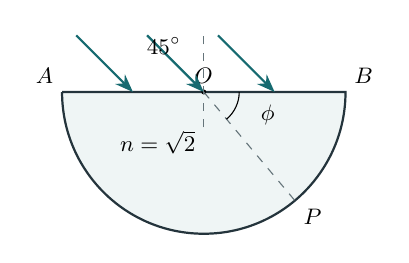
\begin{tikzpicture}[scale=.9,transform shape]
\fill[accent!7] (-2,0) arc(180:360:2)--cycle;\draw[object] (-2,0)--(2,0) arc(0:-180:2);\fill (0.00000,0.00000) circle(.035);\node[above] at (0.00000,0.00000) {$O$};\node[above left] at (-2.00000,0.00000) {$A$};\node[above right] at (2.00000,0.00000) {$B$};\draw[motion] (-1.80000,0.80000)--(-1.00000,0.00000);\draw[motion] (-0.80000,0.80000)--(0.00000,0.00000);\draw[motion] (0.20000,0.80000)--(1.00000,0.00000);\draw[guide] (0.00000,-0.50000)--(0.00000,0.90000);\node[left] at (-0.20000,0.65000) {$45^\circ$};\draw[guide] (0.00000,0.00000)--(1.28558,-1.53209);\node[below right] at (1.28558,-1.53209) {$P$};\draw[thin] (.5,0) arc(0:-50:.5);\node[right] at (0.67973,-0.31696) {$\phi$};\node[above] at (-0.65000,-1.00000) {$n=\sqrt2$};
\end{tikzpicture}
\figcaption{图光1.1\quad 平直面入射及下半圆的位置角}
\end{minipage}\end{center}

\Needspace{6\baselineskip}\subsection*{解答}


取图光1.1中的圆心$O$为原点，平直表面为$x$轴，玻璃位于下半平面。入射光向右下方传播。设光线进入玻璃后的折射角为$r$，折射定律给出
\[
\sin45^\circ=\sqrt2\sin r,\qquad r=30^\circ.
\]
因此玻璃中的光线均沿与$x$轴成$-60^\circ$的方向传播。解图光1.1A先标出平面入口的折射角和左边缘光线AD；随后在B图的圆弧点重新画半径法线，不能继续用入口的竖直法线判断透射。
\begin{center}\begin{minipage}{.98\linewidth}\centering
\begin{tikzpicture}[scale=1.12,font=\small]
\fill[accent!5](-2,0)arc(180:360:2)--cycle;
\draw[object](-2,0)--(2,0)arc(0:-180:2);
\coordinate(O)at(0,0);\coordinate(A)at(-2,0);\coordinate(B)at(2,0);
\coordinate(D)at(-1,-1.73205081);\coordinate(H)at(1,-1.73205081);
\draw[guide](0,.85)--(0,-1.05);
\draw[motion](-1.05,1.05)--(O)--(H);
\draw[motion](A)--(D);\draw[guide](O)--(D);
\draw[motion](1.63299316,0)--(1.93185165,-.51763809);
\draw[accent,line width=1.3pt](0:2.07)arc(0:-120:2.07);
\draw(0,.45)arc(90:135:.45);\node[above left]at(-.12,.58){$45^\circ$};
\draw(0,-.62)arc(-90:-60:.62);\node at(.19,-.85){$r$};
\node[above right]at(O){$O$};\node[above left]at(A){$A$};\node[above right]at(B){$B$};
\node[below left]at(D){$D:\ \phi=120^\circ$};\node[below right]at(H){$H:\ \phi=60^\circ$};
\node[align=left,anchor=west]at(3.2,-.5){入口：$r=30^\circ$\\内部平行方向$-60^\circ$\\$AO=OD=R$\\$\angle OAD=\angle ADO=60^\circ$\\$\angle AOD=60^\circ$\\受照弧：$0<\phi<120^\circ$};
\end{tikzpicture}
\figcaption{解图光1.1A\quad 入口折射与左端边缘光线AD，边缘点D限定首次受照弧}
\end{minipage}\end{center}
图A中的边缘光线由A进入后沿AD传播。因AO水平向右，AD向右下方，$\angle OAD=60^\circ$；又因$OA=OD=R$，三角形AOD为等腰三角形，故
\[
\angle ADO=60^\circ,\qquad
\angle AOD=180^\circ-2\times60^\circ=60^\circ .
\]
从右侧半径OB向下计角时，D的位置为$\phi_D=180^\circ-60^\circ=120^\circ$。圆心角 $60^\circ=\angle AOD$ 从左侧半径量起，从右侧半径量出的 $\phi_D$ 与它互补。

先判断哪些圆弧点实际受到照明。最靠左的入射点为$A=(-R,0)$，这条边缘光线与圆周再次相交于$\phi=120^\circ$处；另一端的极限光线从$B=(R,0)$进入，对应$\phi\to0^\circ$。故用从右端量起的角度表示，第一次受照弧段为
\[
0<\phi<120^\circ.
\]
可直接验证：若$P=(R\cos\phi,-R\sin\phi)$，将光线向上反延至平面，交点横坐标为
\[
x_0=R\cos\phi-\frac{R\sin\phi}{\sqrt3}.
\]
反延的计算也可逐步写出：设入口为$E=(x_0,0)$，内部光线的单位方向为$\vect d=(1/2,-\sqrt3/2)$，于是
\[
P=E+\ell\vect d,\quad
-R\sin\phi=-\ell\sqrt3/2,\quad
\ell=\frac{2R\sin\phi}{\sqrt3},\quad
R\cos\phi=x_0+\ell/2.
\]
消去$\ell$即得前面的$x_0$。若从入口直接求首次圆弧交点，方程
\[
(x_0+\ell/2)^2+3\ell^2/4=R^2
\]
有唯一正根
\[
\ell=\frac{-x_0+\sqrt{4R^2-3x_0^2}}2\quad(-R<x_0<R).
\]
从而AD确实是左端边缘界，不能把反向延长线穿过其他区域的圆弧点算入。要求$-R<x_0<R$，在下半圆内恰给出上述区间。\begin{center}\begin{minipage}{.97\linewidth}\centering
\begin{tikzpicture}[scale=1.12,font=\small]
\fill[accent!5](-2,0)arc(180:360:2)--cycle;
\draw[object](-2,0)--(2,0)arc(0:-180:2);
\coordinate(O)at(0,0);\coordinate(Cone)at(1.93185165,-.51763809);\coordinate(Ctwo)at(-.51763809,-1.93185165);
\coordinate(H)at(1,-1.73205081);
\draw[guide](O)--(2.31822198,-.62116571);\draw[guide](O)--(-.62116571,-2.31822198);
\draw[motion](1.63299316,0)--(Cone);
\draw[motion](-1.63299316,0)--(Ctwo);
\draw[motion](O)--(H)--(1.25,-2.16506351);
\draw[force](Cone)--(1.6212688,-1.67674908);
\draw[force](Ctwo)--(.6414729,-2.2424345);
\draw[accent,line width=1.5pt](-15:2.07)arc(-15:-105:2.07);
\fill(Cone)circle(.035);\fill(Ctwo)circle(.035);\fill(H)circle(.035);
\node[above]at(O){$O$};\node[above right]at(Cone){$C_1$};\node[below left]at(Ctwo){$C_2$};
\node[right]at(1.25,-1.65){$H$};
\node[align=left,anchor=west]at(3.2,-.7){两半径为圆弧外法线\\$C_1:\phi=15^\circ,\ i=45^\circ$\\$H:\phi=60^\circ,\ i=0$\\$C_2:\phi=105^\circ,\ i=45^\circ$\\棕线：两临界切向极限\\粗弧内部：首次到达即可透射};
\end{tikzpicture}
\figcaption{解图光1.1B　两临界点的入射光与半径法线，以及切向透射极限。H处正入射，粗弧只表示两临界点之间的首次透射范围。}
\end{minipage}\end{center}


圆弧外法线的方向角为$-\phi$，而光线的方向角为$-60^\circ$，于是
\[
i=|\phi-60^\circ|.
\]
玻璃射向空气的临界角为
\[
i_c=\arcsin\frac1{\sqrt2}=45^\circ.
\]
解图光1.1B 中，入口折射决定玻璃内的固定传播方向，外法线 $\vect n=(\cos\phi,-\sin\phi)$ 则随位置转动。两者的点积给出入射角：
\[
\vect d\cdot\vect n
=\tfrac12\cos\phi+\tfrac{\sqrt3}{2}\sin\phi
=\cos(\phi-60^\circ)=\cos i.
\]
在已确定的受照弧$0<\phi<120^\circ$上，$|\phi-60^\circ|<60^\circ<90^\circ$，故此处选用的入射角确为$|\phi-60^\circ|$，不是其补角。由$i_c=45^\circ$分成两支临界条件：
\[
\phi-60^\circ=-45^\circ\Rightarrow\phi_{C_1}=15^\circ,\qquad
\phi-60^\circ=+45^\circ\Rightarrow\phi_{C_2}=105^\circ.
\]
两临界点都真实受照，它们之间又没有不可达的圆弧点，才可以连成一段透射弧。

要有传播到空气中的透射光，须$i<i_c$，因而
\[
\boxed{15^\circ<\phi<105^\circ}.
\]
该区间已包含在受照弧段内，弧长所对圆心角为$90^\circ$。在两个端点，折射光沿表面切线传播，应作为临界边界；若把切向极限也计入“透出”，可将区间端点列入，但不能将它当成具有有限法向能流的透射光束。若改从左端$A$向右计角$\phi_L=180^\circ-\phi$，同一弧段写作$75^\circ<\phi_L<165^\circ$。

\begin{center}\begin{minipage}{.97\linewidth}\centering
\begin{tikzpicture}[x=.07cm,y=.045cm,font=\small]
\path[fill=accent!8](15,0)rectangle(105,72);
\path[fill=gray!12](120,0)rectangle(130,72);
\draw[axis](0,0)--(136,0)node[right]{$\phi/(^\circ)$};
\draw[axis](0,0)--(0,79)node[above]{$i/(^\circ)$};
\draw[traj](0,60)--(60,0)--(120,60);
\draw[guide](120,60)--(130,70);
\draw[warm,dashed](0,45)--(130,45);
\foreach \x in {0,15,60,105,120}{\draw(\x,0)--(\x,-2)node[below]{$\x$};}
\foreach \y in {45,60}{\draw(0,\y)--(-2,\y)node[left]{$\y$};}
\draw[guide](15,0)--(15,45);\draw[guide](105,0)--(105,45);
\draw[accent,fill=white](15,45)circle(.055cm);\draw[accent,fill=white](105,45)circle(.055cm);
\node[above]at(66,73){$i=|\phi-60^\circ|,\quad i_c=45^\circ$};
\node[align=center]at(67,-20){浅蓝带内的实线满足$i<i_c$；临界空心点不列入\\灰区不能由平直面入口首次照到，延线只作角度比较};
\end{tikzpicture}
\figcaption{解图光1.1C　受照条件与临界角条件的交集。蓝色角区中的实线低于临界水平线，灰区则不属于首次受照弧。}
\end{minipage}\end{center}

解图光1.1C把两个筛选条件放在同一横轴上：实线先限定$0<\phi<120^\circ$，再取$i<45^\circ$。左段$0<\phi<15^\circ$和右段$105^\circ<\phi<120^\circ$虽有入射光，却发生全反射；$\phi>120^\circ$则连第一次入射都没有，两者应分别说明。

还可直接按从左端量起的$\phi_L$复算临界角，避免只靠最后换算区间。图A中$\angle AOD=60^\circ$为受照边缘，所以受照范围为$60^\circ<\phi_L<180^\circ$。固定内部方向与半径法线的夹角在两临界位置取$\pm i_c$，分别给
\[
\phi_{L,c1}=180^\circ-(60^\circ+45^\circ)=75^\circ,\qquad
\phi_{L,c2}=180^\circ-(60^\circ-45^\circ)=165^\circ .
\]
它们仍位于受照范围内。由$\phi_L=180^\circ-\phi$，15度的右侧临界点对应165度的左侧角，105度对应75度，因变换反向，转换上下界时必须交换次序。

本题的90度是透光弧所张圆心角，不是单根光线的偏向角，也不是入射光在入口上所占比例。透光圆弧两端所对应的入口为
\[
x_{0,C_1}=R\sqrt{\frac23},\qquad
x_{0,C_2}=-R\sqrt{\frac23}.
\]
所以首次可透出的入口横坐标范围为$|x_0|<R\sqrt{2/3}$。这与图B中两条临界内部平行光线吻合，也给出对圆弧位置答案的独立检查。


\Needspace{13\baselineskip}

\pdfbookmark[2]{第 2 题 充液玻璃管的表观壁厚}{q2}

\section*{第 2 题\quad 充液玻璃管的表观壁厚}\label{q:2}

内半径$r$、外半径$R$的圆柱玻璃管，玻璃折射率为$n_1>1$，管内充满折射率$n_2\ge1$的发光液体。观察者在空气中从侧面远处观察。求管壁的表观厚度恰好消失时$r$与$R$应满足的条件，并讨论$n_2<n_1$和$n_2\ge n_1$两种情形。

\begin{center}\begin{minipage}{.98\linewidth}\centering
\begin{tikzpicture}[scale=.9,transform shape]
\draw[object] (0.00000,0.00000) circle(2.00000);\draw[object] (0.00000,0.00000) circle(1.50000);\draw[<->,thin,color=muted] (0.00000,0.00000)--(2.00000,0.00000);\node[below] at (1.00000,0.00000) {$R$};\draw[<->,thin,color=muted] (0.00000,0.00000)--(-1.14907,0.96418);\node[above] at (-0.57453,0.48209) {$r$};\node[above] at (-0.15000,1.05000) {$n_2$};\node[above] at (1.65000,0.60000) {$n_1$};\node[above] at (2.70000,-0.20000) {空气};\node[below] at (0.00000,-2.50000) {远处观察};
\end{tikzpicture}
\figcaption{图光1.2\quad 同心玻璃管及发光液体}
\end{minipage}\end{center}

\Needspace{6\baselineskip}\subsection*{解答}


图光1.2中管轴垂直纸面。远处观察对应近乎平行的出射光；要使发光液体的轮廓扩展到管的最外边缘，边缘$M$处必须存在沿切线$MN$出射的极限光线。解图光1.2A中S是液体内的发光点，P是光进入玻璃的内界面点，PM才是玻璃内的直线光段；P不能与液体深处的发光位置混淆。
\begin{center}\begin{minipage}{.98\linewidth}\centering
\begin{tikzpicture}[scale=1.05,font=\small]
\draw[object](0,0)circle(2);\draw[object](0,0)circle(1.6);
\coordinate(O)at(0,0);\coordinate(M)at(-2,0);\coordinate(P)at(-1.54810653,.40418581);\coordinate(S)at(-1.31920865,.79162065);
\draw[guide](O)--(-2.35,0);\draw[guide](O)--(-1.93513316,.50523226);
\draw[motion](S)--(P)--(M)--(-2,-2.7);
\fill(P)circle(.035);\fill(M)circle(.035);\fill(S)circle(.035);\fill(O)circle(.025);
\node[right]at(O){$O$};\node[above left]at(P){$P$};\node[above right]at(S){$S$};
\node[left]at(M){$M$};\node[below]at(-2,-2.7){$N$};
\draw ($(P)+(165.367625:.28)$)arc(165.367625:221.810315:.28);
\node[left]at(-2.03,.36){$\alpha$};
\draw ($(P)+(-14.632375:.25)$)arc(-14.632375:59.425256:.25);
\node at(-1.17,.61){$j$};
\draw(-1.55,0)arc(0:41.810315:.45);
\node[below]at(-1.32,.08){$i_c$};
\node at(.45,.75){液体$n_2$};\node at(1.72,.65){$n_1$};
\node[align=left,anchor=west]at(3,-.55){S为液内发光点，P在内界面\\MN为外缘切向出射极限\\半径OM、OP分别是两处法线\\图取$R=2,\ r=1.6$\\$n_1=1.5,\ n_2=1.3$\\$i_c=41.81^\circ,\ \alpha=56.44^\circ$\\液体入射角$j=74.06^\circ$};
\end{tikzpicture}
\figcaption{解图光1.2A\quad 边缘切向光线反推内界面的可供方向}
\end{minipage}\end{center}
设$PM$与外表面法线$OM$的夹角为$i_c$，与内表面法线$OP$的锐角为$\alpha$。由$M$处切向出射条件，
\[
n_1\sin i_c=1,\qquad \sin i_c=\frac1{n_1}.
\]
这里$\alpha$是PM与OP延长方向的锐角，三角形在P处的内角实际为$\pi-\alpha$，不是$\alpha$；因此完整正弦定理写为
\[
\frac r{\sin i_c}=\frac R{\sin(\pi-\alpha)}
=\frac R{\sin\alpha}.
\]
M处之所以必须用切向极限，是因为选定观察方向后，外圆投影最左点的半径OM正好与出射方向MN垂直。内界面的位置P再由这一外缘光线反推，不能任取一条近轴光线代表边缘。

在三角形$OPM$中，用正弦定理或光线相对圆心的垂距相等可得
\[
r\sin\alpha=R\sin i_c,\qquad
\sin\alpha=\frac{R}{n_1r}.
\]
所得角度确定了玻璃内的方向，还要检查液体折射出的光能否具有这个方向。若液体内的入射角为$j$，内界面满足
\[
n_2\sin j=n_1\sin\alpha.
\]
要有这样的PM，首先必须$\sin\alpha\le1$，即玻璃内的这条直线确实能交到半径r的内圆；其次还须能找到实的液体入射角j。把外缘条件代入内界面折射式，立即得到
\[
\sin j=\frac{n_1}{n_2}\sin\alpha
=\frac R{n_2r}.
\]
所以几何可达与液体可供方向分别要求$R\le n_1r$和$R\le n_2r$。下面按$n_2$与$n_1$的相对大小展开这两个限制，不能只保留较熟悉的玻璃向空气临界角。

当$n_2<n_1$时，液体射入玻璃的折射角最多为
\[
\alpha_{\max}=\arcsin(n_2/n_1).
\]
所需$\alpha$不应大于它，因此
\[
\frac{R}{n_1r}\le\frac{n_2}{n_1},\qquad
\boxed{\frac Rr\le n_2\quad(n_2<n_1)}.
\]
在这一分支，$j\to90^\circ$时内界面折射定律为$n_2\sin90^\circ=n_1\sin\alpha_{\max}$。由于$n_2/n_1<1$，所需$\alpha$的上限已经比几何90度更严格，故$n_2$控制结果；不能用“玻璃内可画出PM”代替这一供光条件。

当$n_2\ge n_1$时，玻璃中的折射方向可以逼近$\alpha=90^\circ$，故只需
\[
\frac{R}{n_1r}\le1,\qquad
\boxed{\frac Rr\le n_1\quad(n_2\ge n_1)}.
\]
当$n_2>n_1$时，液体一侧的透射角域截止于$j_c=\arcsin(n_1/n_2)$。在$j<j_c$的范围内增大$j$，玻璃中的$\alpha$随之增大；$j\to j_c$时，$\alpha\to90^\circ$。越过$j_c$后，光在液体与玻璃的界面发生全反射。若$n_2=n_1$，光线直穿内界面，入射线趋近内圆切线时也得到同一上限。

合写为
\[
\boxed{1<\frac Rr\le \min(n_1,n_2)}.
\]
该条件描述发光区轮廓能覆盖整个外径的几何极限。等号对应某一界面上的掠射极限；讨论实际观察的亮度时，不能由“轮廓达到外缘”推断边缘亮度与中央相同。若$R/r$大于上述上限，靠近外缘存在无法从液体直接到达观察方向的光线，仍能分辨管壁。


上述条件也充分。若$R\le\min(n_1,n_2)r$，从M沿玻璃内临界方向向后追踪，直线到圆心的垂距为$h=R\sin i_c=R/n_1\le r$，所以可到达内圆；在最近的内界面交点P处再取$j=\arcsin[R/(n_2r)]$，即可反推一条液体中的入射光线。严格不等号给有限传播的可透射路径，等号作为界面掠射或相切的轮廓闭包。

为了确认不只最外一点可到，还可求整个表观发光半径。对任意同心界面上的光线，令
\[
b=n\,s\sin\eta ,
\]
其中s是该界面半径，$\eta$是光线与当地半径法线的夹角。直线段到圆心的垂距是$s\sin\eta$，同一介质内它不变；界面上又有$n\sin\eta$连续，故同一条光路的b在两次折射前后不变。b具有长度量纲，不是无量纲折射率本身。

远处沿竖直方向观察，在空气中$b=|x_{\rm obs}|$。若要反推到液体，必须同时满足
\[
b\le R,\qquad b\le n_1r,\qquad b\le n_2r .
\]
第一式保证外圆有交点，第二式保证玻璃内反向光线能碰到内圆，第三式保证液体中存在实入射角。由此得到表观发光半径a和每侧表观壁厚w：
\[
a=\min\{R,n_1r,n_2r\},\qquad
w=R-a=\max\{0,R-\min(n_1,n_2)r\}.
\]
当$a=R$时整个外径均可由发光液体的光路覆盖，就恢复前面的壁厚消失条件。所有比极限b更小的位置也有可供路径，这补足了只检验最外缘时的存在性说明。
\begin{center}\begin{minipage}{.97\linewidth}\centering
\begin{tikzpicture}[x=4cm,y=1cm,font=\small]
\node[align=center]at(0,1.7){固定$n_1=1.5,\ n_2=1.3$，观察平面位置$x_{\rm obs}/R$\\色带只示光路存在范围，不给亮度分布};
\path[fill=gray!30](-1,.8)rectangle(1,1.08);
\path[fill=accent!40](-.91,.8)rectangle(.91,1.08);
\draw[object](-1,.8)rectangle(1,1.08);
\foreach \x/\v in {-1/-1,0/0,1/1}{\draw(\x,.8)--(\x,.7)node[below]{$\v$};}
\node[align=left,anchor=west]at(1.2,.95){$r/R=0.70$\\$a/R=0.91$\\每侧仍见$0.09R$};
\path[fill=gray!30](-1,-1)rectangle(1,-.72);
\path[fill=accent!40](-1,-1)rectangle(1,-.72);
\draw[object](-1,-1)rectangle(1,-.72);
\foreach \x/\v in {-1/-1,0/0,1/1}{\draw(\x,-1)--(\x,-1.1)node[below]{$\v$};}
\node[align=left,anchor=west]at(1.2,-.85){$r/R=0.80$\\$a/R=1$\\发光轮廓覆盖整个外径};
\end{tikzpicture}
\figcaption{解图光1.2B　同一玻璃和液体下，两种内外半径比的表观轮廓。灰色端带标出液体直达光线到不了的壁区，色带标出轮廓的可见范围。}
\end{minipage}\end{center}

解图光1.2B固定$n_1=1.5,n_2=1.3$。上图$r/R=0.70$时，$a/R=\min(1,1.05,0.91)=0.91$，每侧仍有$0.09R$表观壁区；下图$r/R=0.80$时，$a/R=\min(1,1.20,1.04)=1$，发光轮廓延至外缘。两个例子都不是把物理壁厚$R-r$直接缩放成表观厚度，控制量是折射与几何可达性共同允许的最大b。
\begin{center}\begin{minipage}{.97\linewidth}\centering
\begin{tikzpicture}[x=12cm,y=3cm,font=\small]
\path[fill=accent!12](.66666667,1)--(.66666667,.5)--plot[domain=.66666667:1,samples=90](\x,{1/\x-1})--(1,1)--cycle;
\draw[axis](.5,0)--(1.06,0)node[right]{$\rho=r/R$};
\draw[axis](.5,0)--(.5,1.13)node[above]{$n_2$};
\foreach \x/\v in {.5/.5,.66666667/{2/3},.8/.8,1/1}{\draw(\x,0)--(\x,-.025)node[below]{$\v$};}
\foreach \y/\v in {0/1,.5/1.5,1/2}{\draw(.5,\y)--(.49,\y)node[left]{$\v$};}
\draw[guide](.5,.5)--(1,.5);
\draw[traj](.66666667,1)--(.66666667,.5);
\draw[traj,domain=.66666667:1,samples=90]plot(\x,{1/\x-1});
\fill[warm](.7,.3)circle(.045cm);\node[below left]at(.7,.3){B上};
\fill[accent](.8,.3)circle(.045cm);\node[above right]at(.8,.3){B下};
\node[above]at(.8,1.13){图取$n_1=1.5$};
\node[align=left,anchor=west]at(1.18,.6){浅蓝：几何轮廓覆盖外径\\$n_2<1.5:\ \rho\ge1/n_2$\\$n_2\ge1.5:\ \rho\ge2/3$\\两段边界在$n_2=n_1$连接\\真实管壁另需$\rho<1$};
\end{tikzpicture}
\figcaption{解图光1.2C　固定玻璃折射率1.5的条件图。浅蓝区域满足两次折射的方向存在性，B中的两个例子位于分界两侧。}
\end{minipage}\end{center}

在解图光1.2C中，$\rho=r/R$。液体折射率较低时边界为$\rho=1/n_2$；提高到$n_2=n_1$后，边界固定为$\rho=1/n_1$，再提高$n_2$也不能让玻璃内的直线穿过它本来碰不到的内圆。若$n_2=1$，条件要求$\rho\ge1$，与非零厚度的$\rho<1$冲突；因此不能靠同折射率为空气的发光介质消去一个有有限厚度的管壁轮廓。

本题只判几何发光轮廓。界面的透射率、液体吸收和发光分布会改变亮度，但不允许把违反上述方向存在性的位置宣称为液体的直达出射光；在掠射边界也不能从a达到R推断有与中央相同的边缘强度。


\Needspace{13\baselineskip}

\pdfbookmark[2]{第 3 题 水滴的一次内反射与最小偏向}{q3}

\section*{第 3 题\quad 水滴的一次内反射与最小偏向}\label{q:3}

一条光线从空气射入折射率$n>1$的球形水滴，经过一次内表面反射后再射出。入射角为$\theta$，折射角为$r$，光线传播方向沿图示同一转向累计的偏转量记为$\delta$，不将超过$\pi$的累计量折回为两射线间的较小夹角。判断内反射是否为全反射，并求$\delta$取得内部极小值时$\theta$满足的条件；说明该极小值存在的折射率范围。

\begin{center}\begin{minipage}{.98\linewidth}\centering
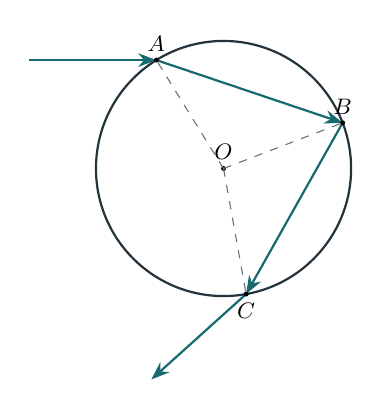
\begin{tikzpicture}[scale=.9,transform shape]
\draw[object] (0.00000,0.00000) circle(1.80000);\draw[motion] (-2.74821,1.53000)--(-0.94821,1.53000);
\draw[motion] (-0.94821,1.53000)--(1.68045,0.64505);
\draw[motion] (1.68045,0.64505)--(0.31909,-1.77149);
\draw[motion] (0.31909,-1.77149)--(-1.01859,-2.97591);\fill (0.00000,0.00000) circle(.035);\node[above] at (0.00000,0.00000) {$O$};\fill (-0.94821,1.53000) circle(.035);\node[above] at (-0.94821,1.53000) {$A$};\draw[guide] (0.00000,0.00000)--(-0.94821,1.53000);\fill (1.68045,0.64505) circle(.035);\node[above] at (1.68045,0.64505) {$B$};\draw[guide] (0.00000,0.00000)--(1.68045,0.64505);\fill (0.31909,-1.77149) circle(.035);\node[below] at (0.31909,-1.77149) {$C$};\draw[guide] (0.00000,0.00000)--(0.31909,-1.77149);
\end{tikzpicture}
\figcaption{图光1.3\quad 一折射、一次内反射、再折射的光支}
\end{minipage}\end{center}

\Needspace{6\baselineskip}\subsection*{解答}


解图光1.3A中的两条弦AB、BC依次连接入射点$A$、反射点$B$与出射点$C$。由于这些点都在同一个圆周上，弦与两端半径组成等腰三角形，故光线在$B$处的入射角也等于$r$。入口折射定律为
\[
\sin\theta=n\sin r.
\]
对$0\le\theta<90^\circ$，有
\[
\sin r=\frac{\sin\theta}{n}<\frac1n,\qquad
r<\arcsin(1/n)=i_c.
\]
几何中的等角可分别落实到两条弦：$\triangle OAB$给$\angle OAB=\angle ABO=r$，反射定律又给$\angle OBC=r$，再由$\triangle OBC$得$\angle BCO=r$。所以C处的内部入射角仍为r，外部折射角也回到$\theta$。这既说明B的全反射比较为何能使用入口数据，也说明最后一次偏折为何与第一次相同。

因此$B$处不满足全反射条件，只发生部分反射；另一部分能量会在$B$直接透出。本题继续追踪反射支，透射支携带的能量则从该处离开水滴。
\begin{center}\begin{minipage}{.98\linewidth}\centering
\begin{tikzpicture}[scale=.9,font=\small]
\draw[object](0,0)circle(1.8);
\coordinate(A)at(-0.94820884,1.53000000);\coordinate(B)at(1.68044887,0.64505162);\coordinate(C)at(0.31909079,-1.77149120);
\draw[motion](-2.74820884,1.53000000)--(A)--(B)--(C)--(-0.90711222,-2.87554109);
\draw[force](B)--(2.95469354,-0.32257462);
\draw[guide](0,0)--(-1.30852820,2.11140000);\draw[guide](0,0)--(B);\draw[guide](0,0)--(0.44034529,-2.44465785);
\node[below left]at(0,0){$O$};
\node[above left]at(A){$A$};\node[above right]at(B){$B$};\node[right]at(C){$C$};
\draw ($(A)+(121.78833062:.43)$)arc(121.78833062:180:.43);\node at(-1.55,1.9){$\theta$};
\draw ($(A)+(-58.21166938:.43)$)arc(-58.21166938:-18.60601699:.43);\node at(-.46,1.12){$r$};
\draw ($(B)+(161.39398301:.4)$)arc(161.39398301:200.99963540:.4);\node at(1.08,.65){$r$};
\draw ($(B)+(200.99963540:.4)$)arc(200.99963540:240.60528780:.4);\node at(1.18,.15){$r$};
\draw ($(C)+(-138.00072919:.4)$)arc(-138.00072919:-79.78905981:.4);\node at(.08,-2.34){$\theta$};
\node[below right]at(2.75,-1.0){B处透射支};
\node[align=left,anchor=west]at(4.15,.45){$OA=OB=OC$\\两条滴内弦：AB、BC\\A折射，B部分反射，C折射\\每条弦两端夹半径角相同\\图取$n=4/3,\ \sin\theta=0.85$\\几何示例，非驻值角图};
\end{tikzpicture}
\figcaption{解图光1.3A\quad 同一球面弦两端角相等，内反射另有透射支}
\end{minipage}\end{center}
\begin{center}\begin{minipage}{.97\linewidth}\centering
\begin{tikzpicture}[scale=.82,font=\small]
\draw[motion](0,0)--(2.3,0)node[above]{$\vect k_0$};
\draw[motion](0,0)--(2.17979029,-0.73383533) node[right]{$\vect k_1$};
\draw[motion](0,0)--(-1.12889370,-2.00389596) node[below]{$\vect k_2$};
\draw[motion](0,0)--(-1.70925268,-1.53897864) node[above]{$\vect k_3$};
\draw[guide](0,0)--(-2.6,0)node[above left]{反向入射};
\draw(1.3,0)arc(0:-18.60601699:1.3);\node at(1.6,-.26){A};
\draw(-18.60601699:1.65)arc(-18.60601699:-119.39471220:1.65);\node at(.72,-1.87){B};
\draw(-119.39471220:1.12)arc(-119.39471220:-138.00072919:1.12);\node at(-1,-1.25){C};
\draw[->,>=Stealth,color=accent](2.7,0)arc(0:-138.00072919:2.7);
\draw[->,>=Stealth,color=warm](-2.7,0)arc(180:221.99927081:2.7);
\node[below]at(.4,-2.95){$\delta$};\node at(-3,-1.1){$\rho$};
\node[align=left,anchor=west]at(4.15,-1.1){仅平移方向箭头，未增加传播段\\A：$\theta-r$\\B：$\pi-2r$\\C：$\theta-r$\\$\delta=\pi+2\theta-4r$\\水滴示例的反向观察角$\rho=\pi-\delta$};
\end{tikzpicture}
\figcaption{解图光1.3B　三次转折的方向比较。将四个传播方向平移到共同起点，只比较转角；实际传播路径仍是A至B至C。}
\end{minipage}\end{center}


沿有向光路逐次累计偏折：入射折射贡献$\theta-r$，内反射贡献$\pi-2r$，出射折射再贡献$\theta-r$，故
\[
\delta(\theta)=\pi+2\theta-4r(\theta),\qquad
r=\arcsin(\sin\theta/n).
\]
解图光1.3B中$\vect k_0,\vect k_1,\vect k_2,\vect k_3$分别是入射、AB、BC和C出射的方向，不是从圆心再次发出的光线。三个顺时针转折相加后取正的累计大小作为$\delta$；若它超过$\pi$，仍保留累计量，不在求极值途中改换为另一夹角。

在水滴通常的$0<\delta<\pi$分支，还可令反向观察角$\rho=\pi-\delta$、辅助半角$\chi=\rho/2$。由两次折射和一次反射的方向关系，$\chi=2r-\theta$，于是
\[
\delta=\pi-2\chi,\qquad \chi=2r-\theta,
\]
同样给$\delta=\pi-4r+2\theta$。只有在明确选定此分支后，$\rho$才直接是与反向入射方向的正夹角；一般折射率推广仍用前述累计定义。

对入口折射式求导，
\[
\cos\theta=n\cos r\,\frac{\dd r}{\dd\theta},
\qquad
\frac{\dd r}{\dd\theta}
=\frac{\cos\theta}{\sqrt{n^2-\sin^2\theta}}.
\]
将两项通分，分子中的平方项相消：
\[
n\cos r=n\sqrt{1-\sin^2r}
=\sqrt{n^2-\sin^2\theta}>0 .
\]
这里$\theta,r$都取$[0,\pi/2)$内的角，故平方根取正支，后面平方驻值式才不会额外引入负号解。

驻值条件为
\[
\frac{\dd\delta}{\dd\theta}
=2-\frac{4\cos\theta}{\sqrt{n^2-\sin^2\theta}}=0.
\]
两端均为非负数，可以平方并整理：
\[
4\cos^2\theta=n^2-\sin^2\theta
=n^2-1+\cos^2\theta,
\qquad
\boxed{\cos^2\theta=\frac{n^2-1}{3}}.
\]
还应检验它确实是极小值。令$g=\cos\theta/\sqrt{n^2-\sin^2\theta}$，则
\[
g'=-\frac{(n^2-1)\sin\theta}
{(n^2-\sin^2\theta)^{3/2}},
\qquad
\delta''=\frac{4(n^2-1)\sin\theta}
{(n^2-\sin^2\theta)^{3/2}}>0.
\]
故$1<n<2$时存在唯一内部极小值。$n=2$时驻值退至$\theta=0$端点；$n>2$时$\delta'(0)>0$且$\delta''\ge0$，最小值在正入射端点，不存在内部驻值。对水取$n=4/3$，得到$\theta\approx59.39^\circ$、$r\approx40.20^\circ$、$\delta_{\min}\approx137.97^\circ$，相对于反向入射方向的夹角约为$42.03^\circ$。


唯一性还可直接从端点斜率看出。对固定$n>1$，
\[
\delta'(0)=2-\frac4n,\qquad
\lim_{\theta\to(\pi/2)^-}\delta'(\theta)=2 .
\]
又因$\delta''(\theta)>0$对$0<\theta<\pi/2$成立，$\delta'$严格增加。当$1<n<2$时，它由负到正，恰过零一次；当$n=2$时只在左端点为零，随后为正；当$n>2$时从左端已为正。因此不能只凭$\cos^2\theta$形式就把所有$n>1$都判作有内部极小值。

对$n=4/3$，中间数值依次为
\[
\begin{gathered}
\cos^2\theta_*=\frac7{27},\qquad
\theta_*=59.391102^\circ,\qquad
r_*=40.202966^\circ,\\
\chi_*=2r_*-\theta_*=21.014829^\circ,\\
\delta_{\min}=180^\circ-2\chi_*
=137.970341^\circ,\qquad
\rho_*=42.029659^\circ.
\end{gathered}
\]
B处入射角40.20度仍小于水向空气的临界角48.59度，所以方向聚集与全反射是两个不同现象。极值来自相邻入射角的出射方向变得接近，不要求反射率等于1。


\begin{center}\begin{minipage}{.97\linewidth}\centering
\begin{tikzpicture}[x=.075cm,y=.027cm,font=\small]
\draw[axis](0,0)--(96,0)node[right]{$\theta/(^\circ)$};
\draw[axis](0,0)--(0,145)node[above]{$\delta/(^\circ)$};
\foreach \x in {0,30,60,90}{\draw(\x,0)--(\x,-2)node[below]{$\x$};}
\foreach \y/\v in {20/140,60/180,100/220,140/260}{\draw(0,\y)--(-1.5,\y)node[left]{$\v$};}
\draw[traj]plot coordinates {(0.00000000,60.00000000) (0.50000000,59.50000833) (1.00000000,59.00006664) (1.50000000,58.50022492) (2.00000000,58.00053321) (2.50000000,57.50104158) (3.00000000,57.00180015) (3.50000000,56.50285914) (4.00000000,56.00426887) (4.50000000,55.50607973) (5.00000000,55.00834228) (5.50000000,54.51110718) (6.00000000,54.01442528) (6.50000000,53.51834757) (7.00000000,53.02292525) (7.50000000,52.52820972) (8.00000000,52.03425259) (8.50000000,51.54110571) (9.00000000,51.04882118) (9.50000000,50.55745138) (10.00000000,50.06704895) (10.50000000,49.57766686) (11.00000000,49.08935838) (11.50000000,48.60217711) (12.00000000,48.11617701) (12.50000000,47.63141242) (13.00000000,47.14793803) (13.50000000,46.66580897) (14.00000000,46.18508078) (14.50000000,45.70580942) (15.00000000,45.22805132) (15.50000000,44.75186339) (16.00000000,44.27730301) (16.50000000,43.80442810) (17.00000000,43.33329708) (17.50000000,42.86396893) (18.00000000,42.39650319) (18.50000000,41.93096001) (19.00000000,41.46740010) (19.50000000,41.00588483) (20.00000000,40.54647620) (20.50000000,40.08923687) (21.00000000,39.63423019) (21.50000000,39.18152021) (22.00000000,38.73117171) (22.50000000,38.28325019) (23.00000000,37.83782196) (23.50000000,37.39495408) (24.00000000,36.95471442) (24.50000000,36.51717171) (25.00000000,36.08239550) (25.50000000,35.65045623) (26.00000000,35.22142523) (26.50000000,34.79537475) (27.00000000,34.37237799) (27.50000000,33.95250910) (28.00000000,33.53584322) (28.50000000,33.12245652) (29.00000000,32.71242617) (29.50000000,32.30583044) (30.00000000,31.90274865) (30.50000000,31.50326124) (31.00000000,31.10744978) (31.50000000,30.71539700) (32.00000000,30.32718679) (32.50000000,29.94290427) (33.00000000,29.56263579) (33.50000000,29.18646893) (34.00000000,28.81449257) (34.50000000,28.44679690) (35.00000000,28.08347343) (35.50000000,27.72461502) (36.00000000,27.37031594) (36.50000000,27.02067184) (37.00000000,26.67577982) (37.50000000,26.33573842) (38.00000000,26.00064768) (38.50000000,25.67060915) (39.00000000,25.34572590) (39.50000000,25.02610257) (40.00000000,24.71184538) (40.50000000,24.40306216) (41.00000000,24.09986237) (41.50000000,23.80235711) (42.00000000,23.51065920) (42.50000000,23.22488312) (43.00000000,22.94514510) (43.50000000,22.67156310) (44.00000000,22.40425686) (44.50000000,22.14334790) (45.00000000,21.88895954) (45.50000000,21.64121696) (46.00000000,21.40024713) (46.50000000,21.16617893) (47.00000000,20.93914310) (47.50000000,20.71927226) (48.00000000,20.50670096) (48.50000000,20.30156564) (49.00000000,20.10400468) (49.50000000,19.91415842) (50.00000000,19.73216911) (50.50000000,19.55818097) (51.00000000,19.39234017) (51.50000000,19.23479483) (52.00000000,19.08569503) (52.50000000,18.94519282) (53.00000000,18.81344218) (53.50000000,18.69059903) (54.00000000,18.57682122) (54.50000000,18.47226854) (55.00000000,18.37710267) (55.50000000,18.29148715) (56.00000000,18.21558741) (56.50000000,18.14957071) (57.00000000,18.09360611) (57.50000000,18.04786445) (58.00000000,18.01251830) (58.50000000,17.98774193) (59.00000000,17.97371127) (59.50000000,17.97060383) (60.00000000,17.97859869) (60.50000000,17.99787641) (61.00000000,18.02861899) (61.50000000,18.07100977) (62.00000000,18.12523339) (62.50000000,18.19147569) (63.00000000,18.26992366) (63.50000000,18.36076530) (64.00000000,18.46418956) (64.50000000,18.58038624) (65.00000000,18.70954587) (65.50000000,18.85185961) (66.00000000,19.00751914) (66.50000000,19.17671652) (67.00000000,19.35964405) (67.50000000,19.55649418) (68.00000000,19.76745934) (68.50000000,19.99273178) (69.00000000,20.23250347) (69.50000000,20.48696589) (70.00000000,20.75630987) (70.50000000,21.04072546) (71.00000000,21.34040174) (71.50000000,21.65552662) (72.00000000,21.98628668) (72.50000000,22.33286699) (73.00000000,22.69545087) (73.50000000,23.07421975) (74.00000000,23.46935295) (74.50000000,23.88102747) (75.00000000,24.30941779) (75.50000000,24.75469565) (76.00000000,25.21702986) (76.50000000,25.69658607) (77.00000000,26.19352657) (77.50000000,26.70801009) (78.00000000,27.24019152) (78.50000000,27.79022180) (79.00000000,28.35824762) (79.50000000,28.94441125) (80.00000000,29.54885033) (80.50000000,30.17169767) (81.00000000,30.81308103) (81.50000000,31.47312295) (82.00000000,32.15194055) (82.50000000,32.84964531) (83.00000000,33.56634298) (83.50000000,34.30213330) (84.00000000,35.05710991) (84.50000000,35.83136018) (85.00000000,36.62496504) (85.50000000,37.43799889) (86.00000000,38.27052941) (86.50000000,39.12261749) (87.00000000,39.99431711) (87.50000000,40.88567526) (88.00000000,41.79673182) (88.50000000,42.72751953) (89.00000000,43.67806391) (89.50000000,44.64838322) (90.00000000,45.63848844)};
\draw[color=warm,line width=1pt]plot coordinates {(0.00000000,60.00000000) (0.50000000,60.00000952) (1.00000000,60.00007616) (1.50000000,60.00025703) (2.00000000,60.00060928) (2.50000000,60.00119005) (3.00000000,60.00205652) (3.50000000,60.00326588) (4.00000000,60.00487536) (4.50000000,60.00694224) (5.00000000,60.00952382) (5.50000000,60.01267747) (6.00000000,60.01646060) (6.50000000,60.02093068) (7.00000000,60.02614526) (7.50000000,60.03216194) (8.00000000,60.03903841) (8.50000000,60.04683242) (9.00000000,60.05560184) (9.50000000,60.06540459) (10.00000000,60.07629871) (10.50000000,60.08834234) (11.00000000,60.10159372) (11.50000000,60.11611120) (12.00000000,60.13195324) (12.50000000,60.14917843) (13.00000000,60.16784548) (13.50000000,60.18801322) (14.00000000,60.20974065) (14.50000000,60.23308685) (15.00000000,60.25811110) (15.50000000,60.28487278) (16.00000000,60.31343146) (16.50000000,60.34384684) (17.00000000,60.37617879) (17.50000000,60.41048735) (18.00000000,60.44683271) (18.50000000,60.48527524) (19.00000000,60.52587549) (19.50000000,60.56869419) (20.00000000,60.61379224) (20.50000000,60.66123074) (21.00000000,60.71107096) (21.50000000,60.76337438) (22.00000000,60.81820266) (22.50000000,60.87561768) (23.00000000,60.93568150) (23.50000000,60.99845639) (24.00000000,61.06400482) (24.50000000,61.13238947) (25.00000000,61.20367324) (25.50000000,61.27791922) (26.00000000,61.35519074) (26.50000000,61.43555131) (27.00000000,61.51906470) (27.50000000,61.60579485) (28.00000000,61.69580597) (28.50000000,61.78916243) (29.00000000,61.88592887) (29.50000000,61.98617013) (30.00000000,62.08995126) (30.50000000,62.19733754) (31.00000000,62.30839448) (31.50000000,62.42318779) (32.00000000,62.54178342) (32.50000000,62.66424750) (33.00000000,62.79064642) (33.50000000,62.92104676) (34.00000000,63.05551532) (34.50000000,63.19411909) (35.00000000,63.33692530) (35.50000000,63.48400137) (36.00000000,63.63541492) (36.50000000,63.79123377) (37.00000000,63.95152593) (37.50000000,64.11635961) (38.00000000,64.28580322) (38.50000000,64.45992532) (39.00000000,64.63879467) (39.50000000,64.82248020) (40.00000000,65.01105100) (40.50000000,65.20457632) (41.00000000,65.40312558) (41.50000000,65.60676834) (42.00000000,65.81557428) (42.50000000,66.02961324) (43.00000000,66.24895519) (43.50000000,66.47367018) (44.00000000,66.70382841) (44.50000000,66.93950015) (45.00000000,67.18075578) (45.50000000,67.42766575) (46.00000000,67.68030059) (46.50000000,67.93873088) (47.00000000,68.20302724) (47.50000000,68.47326035) (48.00000000,68.74950089) (48.50000000,69.03181959) (49.00000000,69.32028713) (49.50000000,69.61497422) (50.00000000,69.91595153) (50.50000000,70.22328967) (51.00000000,70.53705921) (51.50000000,70.85733067) (52.00000000,71.18417444) (52.50000000,71.51766085) (53.00000000,71.85786009) (53.50000000,72.20484222) (54.00000000,72.55867714) (54.50000000,72.91943460) (55.00000000,73.28718416) (55.50000000,73.66199516) (56.00000000,74.04393672) (56.50000000,74.43307772) (57.00000000,74.82948679) (57.50000000,75.23323225) (58.00000000,75.64438215) (58.50000000,76.06300418) (59.00000000,76.48916572) (59.50000000,76.92293376) (60.00000000,77.36437491) (60.50000000,77.81355536) (61.00000000,78.27054090) (61.50000000,78.73539682) (62.00000000,79.20818796) (62.50000000,79.68897865) (63.00000000,80.17783271) (63.50000000,80.67481338) (64.00000000,81.17998335) (64.50000000,81.69340472) (65.00000000,82.21513895) (65.50000000,82.74524686) (66.00000000,83.28378859) (66.50000000,83.83082361) (67.00000000,84.38641065) (67.50000000,84.95060770) (68.00000000,85.52347198) (68.50000000,86.10505990) (69.00000000,86.69542707) (69.50000000,87.29462824) (70.00000000,87.90271731) (70.50000000,88.51974725) (71.00000000,89.14577013) (71.50000000,89.78083709) (72.00000000,90.42499826) (72.50000000,91.07830280) (73.00000000,91.74079886) (73.50000000,92.41253352) (74.00000000,93.09355282) (74.50000000,93.78390168) (75.00000000,94.48362393) (75.50000000,95.19276226) (76.00000000,95.91135819) (76.50000000,96.63945207) (77.00000000,97.37708305) (77.50000000,98.12428903) (78.00000000,98.88110670) (78.50000000,99.64757147) (79.00000000,100.42371746) (79.50000000,101.20957750) (80.00000000,102.00518308) (80.50000000,102.81056436) (81.00000000,103.62575015) (81.50000000,104.45076788) (82.00000000,105.28564359) (82.50000000,106.13040191) (83.00000000,106.98506607) (83.50000000,107.84965784) (84.00000000,108.72419757) (84.50000000,109.60870414) (85.00000000,110.50319497) (85.50000000,111.40768598) (86.00000000,112.32219163) (86.50000000,113.24672486) (87.00000000,114.18129712) (87.50000000,115.12591834) (88.00000000,116.08059694) (88.50000000,117.04533981) (89.00000000,118.02015230) (89.50000000,119.00503827) (90.00000000,120.00000000)};
\draw[color=muted,line width=1pt]plot coordinates {(0.00000000,60.00000000) (0.50000000,60.09091825) (1.00000000,60.18189142) (1.50000000,60.27297445) (2.00000000,60.36422229) (2.50000000,60.45568987) (3.00000000,60.54743216) (3.50000000,60.63950415) (4.00000000,60.73196083) (4.50000000,60.82485725) (5.00000000,60.91824844) (5.50000000,61.01218951) (6.00000000,61.10673558) (6.50000000,61.20194181) (7.00000000,61.29786340) (7.50000000,61.39455561) (8.00000000,61.49207374) (8.50000000,61.59047315) (9.00000000,61.68980923) (9.50000000,61.79013747) (10.00000000,61.89151339) (10.50000000,61.99399258) (11.00000000,62.09763071) (11.50000000,62.20248352) (12.00000000,62.30860682) (12.50000000,62.41605649) (13.00000000,62.52488850) (13.50000000,62.63515891) (14.00000000,62.74692384) (14.50000000,62.86023953) (15.00000000,62.97516229) (15.50000000,63.09174854) (16.00000000,63.21005477) (16.50000000,63.33013759) (17.00000000,63.45205371) (17.50000000,63.57585994) (18.00000000,63.70161318) (18.50000000,63.82937047) (19.00000000,63.95918892) (19.50000000,64.09112578) (20.00000000,64.22523839) (20.50000000,64.36158423) (21.00000000,64.50022087) (21.50000000,64.64120602) (22.00000000,64.78459748) (22.50000000,64.93045319) (23.00000000,65.07883120) (23.50000000,65.22978969) (24.00000000,65.38338696) (24.50000000,65.53968141) (25.00000000,65.69873160) (25.50000000,65.86059618) (26.00000000,66.02533394) (26.50000000,66.19300378) (27.00000000,66.36366474) (27.50000000,66.53737596) (28.00000000,66.71419673) (28.50000000,66.89418642) (29.00000000,67.07740457) (29.50000000,67.26391080) (30.00000000,67.45376485) (30.50000000,67.64702660) (31.00000000,67.84375603) (31.50000000,68.04401323) (32.00000000,68.24785839) (32.50000000,68.45535184) (33.00000000,68.66655399) (33.50000000,68.88152536) (34.00000000,69.10032656) (34.50000000,69.32301833) (35.00000000,69.54966146) (35.50000000,69.78031686) (36.00000000,70.01504551) (36.50000000,70.25390849) (37.00000000,70.49696694) (37.50000000,70.74428209) (38.00000000,70.99591522) (38.50000000,71.25192769) (39.00000000,71.51238091) (39.50000000,71.77733634) (40.00000000,72.04685550) (40.50000000,72.32099994) (41.00000000,72.59983125) (41.50000000,72.88341103) (42.00000000,73.17180094) (42.50000000,73.46506262) (43.00000000,73.76325773) (43.50000000,74.06644792) (44.00000000,74.37469485) (44.50000000,74.68806013) (45.00000000,75.00660539) (45.50000000,75.33039218) (46.00000000,75.65948204) (46.50000000,75.99393644) (47.00000000,76.33381677) (47.50000000,76.67918440) (48.00000000,77.03010056) (48.50000000,77.38662641) (49.00000000,77.74882302) (49.50000000,78.11675132) (50.00000000,78.49047212) (50.50000000,78.87004609) (51.00000000,79.25553377) (51.50000000,79.64699550) (52.00000000,80.04449148) (52.50000000,80.44808169) (53.00000000,80.85782592) (53.50000000,81.27378377) (54.00000000,81.69601456) (54.50000000,82.12457742) (55.00000000,82.55953119) (55.50000000,83.00093445) (56.00000000,83.44884548) (56.50000000,83.90332229) (57.00000000,84.36442255) (57.50000000,84.83220359) (58.00000000,85.30672242) (58.50000000,85.78803567) (59.00000000,86.27619960) (59.50000000,86.77127007) (60.00000000,87.27330252) (60.50000000,87.78235199) (61.00000000,88.29847303) (61.50000000,88.82171978) (62.00000000,89.35214586) (62.50000000,89.88980442) (63.00000000,90.43474809) (63.50000000,90.98702897) (64.00000000,91.54669860) (64.50000000,92.11380797) (65.00000000,92.68840748) (65.50000000,93.27054694) (66.00000000,93.86027553) (66.50000000,94.45764179) (67.00000000,95.06269362) (67.50000000,95.67547824) (68.00000000,96.29604218) (68.50000000,96.92443127) (69.00000000,97.56069060) (69.50000000,98.20486454) (70.00000000,98.85699667) (70.50000000,99.51712983) (71.00000000,100.18530604) (71.50000000,100.86156650) (72.00000000,101.54595161) (72.50000000,102.23850089) (73.00000000,102.93925304) (73.50000000,103.64824583) (74.00000000,104.36551618) (74.50000000,105.09110008) (75.00000000,105.82503258) (75.50000000,106.56734780) (76.00000000,107.31807891) (76.50000000,108.07725810) (77.00000000,108.84491656) (77.50000000,109.62108450) (78.00000000,110.40579110) (78.50000000,111.19906452) (79.00000000,112.00093186) (79.50000000,112.81141919) (80.00000000,113.63055149) (80.50000000,114.45835267) (81.00000000,115.29484555) (81.50000000,116.14005186) (82.00000000,116.99399219) (82.50000000,117.85668604) (83.00000000,118.72815174) (83.50000000,119.60840652) (84.00000000,120.49746642) (84.50000000,121.39534637) (85.00000000,122.30206009) (85.50000000,123.21762015) (86.00000000,124.14203794) (86.50000000,125.07532368) (87.00000000,126.01748637) (87.50000000,126.96853384) (88.00000000,127.92847273) (88.50000000,128.89730845) (89.00000000,129.87504523) (89.50000000,130.86168609) (90.00000000,131.85723284)};
\draw[guide](59.39110234,0)--(59.39110234,17.97034113)--(0,17.97034113);
\fill[accent](59.39110234,17.97034113)circle(.055cm);
\node[above left]at(59.39110234,17.97034113){$(\theta_*,\delta_{\min})$};
\foreach \y in {45.63848844,120.00000000,131.85723284}{\draw[fill=white](90,\y)circle(.045cm);}
\node[align=left,anchor=west]at(108,105){{\color{accent}$n=4/3$：唯一内部极小}\\{\color{warm}$n=2$：驻值退到端点}\\{\color{muted}$n=2.2$：全程递增}\\$\delta$按同一方向累计\\90度处空心点只示掠射极限};
\end{tikzpicture}
\figcaption{解图光1.3C　三种折射率的累计偏转曲线。内部极小值、端点退化和全程递增分别对应不同参数范围，不能只解驻值方程。}
\end{minipage}\end{center}

解图光1.3C的蓝线在$\theta_*$两侧先降后升；棕线与灰线则从端点开始上升。纵轴为累计$\delta$，部分曲线大于180度时没有折回，因而与上面的$n\ge2$单调性判断一致。若要由实际射线方向报告较小夹角，应在累计光路已确定后另作方向取模，不能混在同一极值函数内。

在水滴驻值附近，若角度统一用弧度，
\[
\delta-\delta_{\min}
=\frac12\delta''(\theta_*)(\theta-\theta_*)^2
+O((\theta-\theta_*)^3),\qquad
\delta''(\theta_*)\simeq2.53546 .
\]
一次项为零，所以两侧小幅改变入口角都可给几乎相同的出射方向。该局部展开解释了角度聚集，但不单独给出光强，也不把B处的部分反射改成全反射。


\Needspace{13\baselineskip}

\pdfbookmark[2]{第 4 题 温度计内径的表观尺寸}{q4}

\section*{第 4 题\quad 温度计内径的表观尺寸}\label{q:4}

\begin{enumerate}
\item 一圆柱玻璃温度计的内、外直径分别为$2r=1\,\mathrm{mm}$、$2R=3\,\mathrm{mm}$，玻璃折射率$n_g=1.5$，外部为空气。从侧面远处观察，求内径的表观尺寸。
\item 另一温度计外径及玻璃折射率相同，内径为$2r=0.1\,\mathrm{mm}$，竖直悬在盛水圆柱烧杯的中心。水的折射率$n_w=4/3$，烧杯壁厚忽略。求从烧杯外侧远处观察时温度计内径和外径的表观尺寸。对细内径作近轴近似，并说明对外径采用的近似。

\item 在前两问中，另行区分两指定射线反延确定的径向虚像构造尺寸与垂直固定远处视线的投影尺寸；给出二者的联系和适用条件。
\end{enumerate}

\begin{center}\begin{minipage}{.98\linewidth}\centering
\begin{tikzpicture}[scale=.9,transform shape]
\draw[object] (0.00000,0.00000) circle(2.00000);\draw[object] (0.00000,0.00000) circle(0.66667);\fill (0.00000,0.00000) circle(.035);\node[below left] at (0.00000,0.00000) {$O$};\draw[<->,thin,color=muted] (-2.40000,-0.66667)--(-2.40000,0.66667);\node[left] at (-2.40000,0.00000) {$2r$};\draw[<->,thin,color=muted] (2.40000,-2.00000)--(2.40000,2.00000);\node[right] at (2.40000,0.00000) {$2R$};\node[above] at (0.00000,-1.30000) {$n_g$};\node[right] at (3.40000,0.00000) {观察};
\end{tikzpicture}
\figcaption{图光1.4\quad 圆柱温度计及内外径}
\end{minipage}\end{center}

\Needspace{6\baselineskip}\subsection*{解答}


\subsubsection*{有限内径的圆柱折射}
解图光1.4A中$P=(0,r)$位于内管上缘；$PM$沿半径向上射出，不发生偏折。另一条从$P$沿内壁切线向右的光线，在外圆$N=(\sqrt{R^2-r^2},r)$折射。其反向延长线与$PM$相交于$Q$，定义径向两射线构造半径$r'=OQ$。有限角度下，这一交点位置与垂直固定视线的投影半宽不是同一个量，先按此构造完整计算，再作投影比较。
\begin{center}\begin{minipage}{.98\linewidth}\centering
\begin{tikzpicture}[scale=1.0,font=\small]
\draw[object](0,0)circle(2);\draw[object](0,0)circle(.66666667);
\coordinate(O)at(0,0);\coordinate(P)at(0,.66666667);\coordinate(N)at(1.88561808,.66666667);\coordinate(Q)at(0,1.01712508);
\draw[motion](P)--(0,2.65)node[above]{$M$};
\draw[motion](P)--(N)--(3.36036,0.39257314);
\draw[guide](Q)--(N);\draw[guide](O)--(2.63986531,.93333333);
\draw ($(N)+(180:.45)$)arc(180:199.47122063:.45);
\draw ($(N)+(-10.52877937:.55)$)arc(-10.52877937:19.47122063:.55);
\node at(1.2,.53){$\phi$};\node at(2.63,.78){$\theta$};
\fill(P)circle(.03);\fill(N)circle(.03);\fill(Q)circle(.03);
\node[below left]at(O){$O$};\node[below left]at(P){$P$};\node[above left]at(Q){$Q$};\node[above]at(N){$N$};
\draw[<->,color=muted](-.95,0)--(-.95,1.01712508)node[midway,left]{$r'=OQ$};
\node[align=left,anchor=west]at(4.15,.55){径向光PM与折射光反延交于Q\\P在内壁，PN沿内壁切向\\$\phi=19.4712^\circ,\ \theta=30^\circ$\\$\Delta=\theta-\phi=10.5288^\circ$\\$2OQ=1.5256876\,{\rm mm}$\\该交点定义径向构造量};
\end{tikzpicture}
\figcaption{解图光1.4A\quad 内壁切向光与径向光确定表观上缘}
\end{minipage}\end{center}
设玻璃内入射角为$\phi$，空气中折射角为$\theta$。由$ON$的几何关系与折射定律，
\[
\sin\phi=\frac rR,\quad
\cos\phi=\frac{\sqrt{R^2-r^2}}R,\quad
\sin\theta=\frac{n_g}{n_e}\frac rR,
\]
其中第一问$n_e=1$。出射光相对水平线向下偏折$\theta-\phi$，反向延至$x=0$，因此
\[
r'=r+\sqrt{R^2-r^2}\tan(\theta-\phi).
\]
将正切差角展开，中间计算为
\[
r'=r+\sqrt{R^2-r^2}
\frac{\sin\theta\cos\phi-\cos\theta\sin\phi}
{\cos\theta\cos\phi+\sin\theta\sin\phi}.
\]
第一问还需$\cos\theta=\sqrt3/2$；$\sin\phi=1/3$、$\cos\phi=\sqrt8/3$、$\sin\theta=1/2$分别代入分子和分母，不能漏掉任一乘积。此两射线构造要求$(n_g/n_e)r/R\le1$，否则切向玻璃光线在外壁不能沿实折射角离开。

此式中$\theta-\phi$要由真实光路判断，不能仅凭“凸面放大”确定正负。代入$r=0.5\,\mathrm{mm}$、$R=1.5\,\mathrm{mm}$，
\[
\sin\phi=\frac13,\qquad
\cos\phi=\frac{\sqrt8}{3},\qquad
\theta=30^\circ.
\]
于是
\[
2r'=2\left[\frac12+\sqrt2
\tan\!\left(30^\circ-\arcsin\frac13\right)\right]\mathrm{mm}
\approx\boxed{1.526\,\mathrm{mm}}.
\]
对径向构造量$2OQ$，直接取近轴近似$2n_gr=1.5\,\mathrm{mm}$会略小，差异来自有限$r/R$。但若测的是垂直固定视线的投影宽度，还必须作下面的几何转换，不能把两个不同量的差值统称为同一测量的近似误差。
\begin{center}\begin{minipage}{.97\linewidth}\centering
\begin{tikzpicture}[scale=.9,font=\small]
\coordinate(O)at(0,0);\coordinate(Q)at(0,4);\coordinate(H)at(0.71861127,3.86643989);
\draw[guide](O)--(Q);
\draw[traj](O)--(H);
\draw[motion](Q)--(5,3.07070679);
\node[below]at(4.1,2.9){出射方向};
\pic[draw,angle radius=3mm]{right angle=O--H--Q};
\draw(0,1.1)arc(90:79.47122063:1.1);
\node[left]at(-.1,1.1){$\Delta$};
\node[below]at(O){$O$};\node[above left]at(Q){$Q$};\node[above right]at(H){$H$};
\node[left]at(0,2.35){$r'=OQ$};
\node[right]at(.42,2.1){$b=OH$};
\node[align=left,anchor=west]at(6.0,2.3){H为O到出射直线的垂足\\$\angle QOH=\Delta$\\$b=r'\cos\Delta$\\$b=(n_g/n_e)r$\\第一问：$2OQ=1.5256876\,{\rm mm}$\\垂直视线投影：$2b=1.5000000\,{\rm mm}$\\三角形统一放大，角度取本题实际值};
\end{tikzpicture}
\figcaption{解图光1.4B　径向构造OQ与垂直出射方向的投影OH。两者相差一个真实差角的余弦因子，有限角度时应分别命名。}
\end{minipage}\end{center}

解图光1.4B中令$\Delta=\theta-\phi$，H为圆心O到出射直线的垂足。直角三角形给$b=OH=OQ\cos\Delta$；再代入A图构造式，有严格恒等式
\[
\begin{aligned}
b&=r\cos(\theta-\phi)+\sqrt{R^2-r^2}\sin(\theta-\phi)\\
 &=R\bigl[\sin\phi\cos(\theta-\phi)+\cos\phi\sin(\theta-\phi)\bigr]\\
 &=R\sin\theta=\frac{n_g}{n_e}r.
\end{aligned}
\]
等价地，$r'=(n_g/n_e)r/\cos\Delta$。这解释了第一问$2OQ=1.5256876\,{\rm mm}$而$2b=1.5000000\,{\rm mm}$为何都能由同一条真实光线得到：它们分别沿径向与垂直视线方向量取。

若固定观察者在远处，从圆柱旋转对称性可将相应的内壁切向光支转到同一观察方向；轮廓半宽应取到该方向的垂距b。因此按固定远处视线的内壁几何轮廓定义，第一问投影直径为$1.5000\,{\rm mm}$；按题图指定两射线交点的径向构造定义，则为$1.5257\,{\rm mm}$，约$1.53\,{\rm mm}$。报告尺寸时必须同时说明是哪一种定义。

有限孔径时，$Q$ 是图 A 所选两射线的交点。换取同一物点发出的其他光线，其反延交点一般会移动。近轴时，光线的方向变化保留到一阶，径向构造与固定视线的投影也在这一阶相合。
\subsubsection*{细内径与同心多层介质}
当$r/R\ll1$时，$\phi\simeq r/R$、$\theta\simeq(n_g/n_e)\phi$，因此
\[
r'\simeq r+R(\theta-\phi)
\simeq\frac{n_g}{n_e}r.
\]
解图光1.4C将玻璃、水和空气的同心界面分开，先在水中形成表观内半径$r_w\simeq(n_g/n_w)r$，再从烧杯侧面折射到空气。解图光1.4C 用 $x/R,y/r$ 放大细束的高度。图示取 $R_b=10R$ 绘制一组光线，两圆柱面的共同圆心为 $O$。
\begin{center}\begin{minipage}{.98\linewidth}\centering
\begin{tikzpicture}[x=.8cm,y=1.4cm,font=\small]
\draw[axis](0,-.55)--(0,2.05)node[above]{$y/r$};
\draw[axis](0,0)--(12.6,0)node[right]{$x/R$};
\node[below left]at(0,0){$O$};
\draw[object,domain=-.5:1.8,samples=60]plot({sqrt(1-(\x/30)^2)},\x);
\draw[object,domain=-.5:1.8,samples=60]plot({sqrt(100-(\x/30)^2)},\x);
\draw[motion](0,1)--(0.99944429,1.00000000)--(9.99999912,-0.12578297)--(12.00000000,-0.45094414);
\draw[guide,color=warm](0.00000000,1.12500978)--(0.99944429,1.00000000);
\draw[guide,color=accent](0.00000000,1.50002203)--(9.99999912,-0.12578297);
\fill(0,1)circle(.035cm);\fill(0.00000000,1.12500978) circle(.035cm);\fill(0.00000000,1.50002203) circle(.035cm);
\node[below left]at(0,1){$P$};
\node[above left]at(0.00000000,1.12500978){$Q_w$};\node[above left]at(0.00000000,1.50002203){$Q_{\rm air}$};
\node[above]at(1,1.85){玻璃外壁};
\node[above]at(6.0,1.5){水$n_w$};
\node[above]at(10,1.85){烧杯外壁};\node[above]at(11.6,1.5){空气};
\draw[<->,color=muted](0,-.4)--(1,-.4)node[midway,below]{$R$};
\draw[<->,color=muted](0,-.75)--(10,-.75)node[midway,below]{$R_b$};
\node[align=center]at(6,-1.55){局部坐标图：纵向以r为单位放大，不能从图上直接量折射角\\图示取$r/R=1/30,\ R_b=10R$，两界面共同圆心O\\$r_w\simeq(n_g/n_w)r,\qquad r_{\rm air}\simeq n_w r_w=n_gr$};
\end{tikzpicture}
\figcaption{解图光1.4C\quad 同心两层的实际近轴光束。横纵单位不同，Q表示各段直线的轴上反延交点，角度由折射式计算。}
\end{minipage}\end{center}
\[
r_{\mathrm{air}}\simeq\frac{n_w}{1}r_w
=n_gr,\qquad
\boxed{2r_{\mathrm{air}}\simeq0.15\,\mathrm{mm}}.
\]
在横截面内，将同心的玻璃外圆柱面和烧杯侧面各自的近轴倍率相乘，中间的 $n_w$ 约去。温度计的外缘半径为 $R$，外轮廓的光从水中经烧杯侧面进入空气。若温度计外径远小于烧杯半径$R_b$，可同样用近轴近似：
\[
\boxed{2R_{\mathrm{air}}\simeq n_w(2R)=4.0\,\mathrm{mm}}.
\]
针对径向虚像构造，第二问没有给$R_b$，所以$4.0\,\mathrm{mm}$应明确标为$R/R_b\ll1$下的近似结果；若烧杯半径与温度计半径可比，可用第一部分的有限角度式，以内物半径$R$、外圆半径$R_b$、折射率比$n_w/1$重新计算。这一有限构造值依赖$R_b$，不能声称对任意烧杯都精确等于4毫米。


第二问的内径有 $r/R=1/30$，玻璃侧切线与外圆柱面法线的夹角很小。用近轴法求温度计的外径时，烧杯侧面的入射角由 $R/R_b$ 决定，取 $R\ll R_b$ 才可展开。令$m=n_g/n_e$、$x=r/R$，前面的精确恒等式给
\[
r'=mr\left[1+\tfrac12(m-1)^2x^2+O(x^4)\right].
\]
因此，径向构造的首项非线性修正与近轴半径的比值为 $O((r/R)^2)$。控制这一修正的是内外半径比。

若另按固定远处视线的轮廓投影定义尺寸，同心界面上$b=n\,s\sin\eta$在各段保持。内壁的玻璃侧切向边界给$b=n_gr$，但还要能穿过温度计外圆和烧杯外圆，因此空气中的半宽上限分别为
\[
a_{\rm inner}=\min\{n_gr,n_wR,R_b\},\qquad
a_{\rm outer}=\min\{n_wR,R_b\}.
\]
本题细内壁有$n_gr=0.075\,{\rm mm}$，另两上限均不更小，所以投影内径为$0.15\,{\rm mm}$。若烧杯半径$R_b\ge n_wR=2\,{\rm mm}$，投影外径就是$4.0\,{\rm mm}$，不需要再令$R/R_b$趋零；若$R<R_b<2\,{\rm mm}$，则被烧杯可见外缘截断，只能达到$2R_b$。这与径向虚像构造所需的近轴或有限角度条件不同，应分别报告，不能把一种尺寸的条件移给另一种。


\Needspace{13\baselineskip}

\pdfbookmark[2]{第 5 题 两平面镜的连续成像与可见范围}{q5}

\section*{第 5 题\quad 两平面镜的连续成像与可见范围}\label{q:5}

两块足够大的平面反射镜$A,B$相交，反射面相对，夹角为$0<\theta<\pi$。在垂直交棱的截面中，交点为$O$，物点$P$与$OA,OB$的夹角分别为$\alpha,\beta$，其中$\alpha+\beta=\theta$。观察者位于两镜之间。
\begin{enumerate}
\item 讨论一般情况下反射像的位置和最多可见像数的确定方法，区分不同方向形成的像与同一观察位置可见的像。
\item 当$\theta=\pi/5,\pi/3,\pi/2$时，各能形成多少个不同反射像，最多可见多少个？写出像的位置，并说明观察方向恰使光路经过交点$O$时的例外。
\end{enumerate}

\begin{center}\begin{minipage}{.98\linewidth}\centering
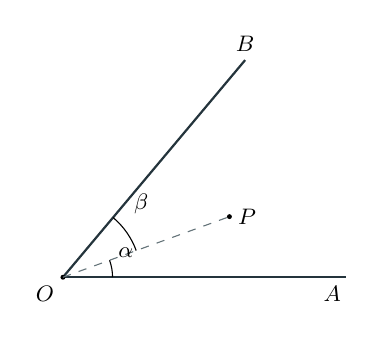
\begin{tikzpicture}[scale=.9,transform shape]
\draw[object] (0.00000,0.00000)--(4.00000,0.00000);\draw[object] (0.00000,0.00000)--(2.57115,3.06418);\fill (0.00000,0.00000) circle(.035);\node[below left] at (0.00000,0.00000) {$O$};\fill (2.34923,0.85505) circle(.035);\node[right] at (2.34923,0.85505) {$P$};\draw[guide] (0.00000,0.00000)--(2.34923,0.85505);\draw[thin] (.7,0) arc(0:20:.7);\draw[thin] (20:1.1) arc(20:50:1.1);\node[above] at (0.88633,0.15628) {$\alpha$};\node[above] at (1.10586,0.77433) {$\beta$};\node[below] at (3.80000,0.00000) {$A$};\node[above] at (2.57115,3.06418) {$B$};
\end{tikzpicture}
\figcaption{图光1.5\quad 镜间物点与两侧夹角}
\end{minipage}\end{center}

\Needspace{6\baselineskip}\subsection*{解答}


各次平面反射都保持到交棱的距离不变，故所有像点都在以$O$为心、$OP=\rho$为半径的圆上。取$OA$方向角为0，$OB$方向角为$\theta$，物点方向角为$\alpha$。镜面反射对方向角的作用为
\[
\mathcal R_A(\varphi)=-\varphi,\qquad
\mathcal R_B(\varphi)=2\theta-\varphi.
\]
从$A$先反射的一列依次为
\[
A_1:-\alpha,\quad A_2:2\theta+\alpha,\quad
A_3:-2\theta-\alpha,\quad A_4:4\theta+\alpha,\ldots;
\]
从$B$先反射的一列为
\[
B_1:2\theta-\alpha,\quad B_2:\alpha-2\theta,\quad
B_3:4\theta-\alpha,\quad B_4:\alpha-4\theta,\ldots.
\]
这些角应保留转动次序，最后再对$2\pi$取模；提前取模并任意继续反射，可能把背面也当作反射面。
\begin{center}\begin{minipage}{.98\linewidth}\centering
\begin{tikzpicture}[scale=.95,font=\small]
\fill[gray!12](0,0)--(180:2.3)arc(180:230:2.3)--cycle;
\draw[guide](0,0)circle(2.3);
\draw[object](0,0)--(3,0)node[right]{$A$};
\draw[object](0,0)--(50:3)node[above]{$B$};
\draw[guide](0,0)--(180:2.65);\draw[guide](0,0)--(230:2.65);
\node[above]at(180:2.65){$A'$};\node[below left]at(230:2.75){$B'$};
\draw[guide](0,0)--(18:2.3);
\draw(.65,0)arc(0:18:.65);\draw(18:1)arc(18:50:1);
\node at(9:.85){$\alpha$};\node at(34:1.2){$\beta$};
\node[below right]at(0,0){$O$};
\draw[guide,color=accent](-18:2.3)--(-118:2.3);
\draw[guide,color=warm](18:2.3)--(118:2.3)--(218:2.3);
\draw[->,color=accent](-18:1.6)arc(-18:-118:1.6);
\draw[->,color=warm](118:1.85)arc(118:218:1.85);
\node at(-68:1.35){$2\theta$};\node at(164:1.6){$2\theta$};
\fill[color=warm](2.18742999,0.71073909)circle(.035);\node at(2.49176807,0.80962453){$ P$};
\fill[color=accent](2.18742999,-0.71073909)circle(.035);\node at(2.49176807,-0.80962453){$ A_1$};
\fill[color=accent](-1.07978459,2.03077946)circle(.035);\node at(-1.23001549,2.31332269){$ A_2$};
\fill[color=accent](-1.07978459,-2.03077946)circle(.035);\node at(-1.23001549,-2.31332269){$ A_3$};
\fill[color=accent](-1.81242473,-1.41602139)circle(.035);\node at(-2.06458817,-1.61303307){$ A_4$};
\fill[color=muted](0.32009813,2.27761656)circle(.035);\node at(0.36463352,2.59450234){$ B_1$};
\fill[color=muted](0.32009813,-2.27761656)circle(.035);\node at(0.36463352,-2.59450234){$ B_2$};
\fill[color=muted](-2.29859890,-0.08026884)circle(.035);\node at(-2.61840397,-0.44){$ B_3$};
\node[align=left,anchor=west]at(3.7,.5){示例：$\theta=50^\circ,\ \alpha=18^\circ$\\奇数A项向顺时针推进\\偶数A项向逆时针推进\\每次跨过同奇偶项，角距增$2\theta$\\灰扇区为两镜共同背面\\末级$A_4,B_3$进入灰扇区\\反射序号须先保留，再作同位去重};
\end{tikzpicture}
\figcaption{解图光1.5A\quad 圆周上的两列像及同奇偶项的圆弧递推}
\end{minipage}\end{center}

\subsubsection*{从逐级圆弧推进到末级像}
解图光1.5A用$\theta=50^\circ,\alpha=18^\circ$显示同一圆上的两列像，灰区由两镜反向延长线$OA',OB'$围成。下列弧距按成像次序指定顺、逆时针，不是任取较小圆弧；暂取$OP=1$，弧距便等于相应圆心角。A列前五项逐次给
\[
\begin{aligned}
\widehat{PA_1}&=2\alpha,\\
\widehat{PA_2}&=\beta+\widehat{BA_2}
=\beta+\widehat{BA_1}=\beta+(\beta+2\alpha)=2\theta,\\
\widehat{PA_3}&=\alpha+\widehat{AA_3}
=\alpha+\widehat{AA_2}
=\alpha+\theta+\widehat{BA_1}
=\alpha+\theta+(\theta+\alpha)=2\alpha+2\theta,\\
\widehat{PA_4}&=\beta+\widehat{BA_4}
=\beta+\theta+\widehat{AA_2}\\
&=\beta+2\theta+\widehat{BA_1}
=\beta+2\theta+(\theta+\alpha)=4\theta,\\
\widehat{PA_5}&=\alpha+\widehat{AA_4}
=\alpha+\theta+\widehat{BA_3}
=\alpha+\theta+(3\theta+\alpha)=2\alpha+4\theta.
\end{aligned}
\]
这里相邻两次反射的镜面对称分别给$\widehat{BA_2}=\widehat{BA_1}$、$\widehat{AA_3}=\widehat{AA_2}$等关系。因而A列奇数项沿顺时针每隔$2\theta$推进，偶数项沿逆时针每隔$2\theta$推进，不能按脚标顺序把所有点都向同一方向累加。B列交换$\alpha,\beta$即可得到同样结构。

非退化位置中，若A列最后一项为奇数$2n+1$，进入灰区的判据为
\[
2\alpha+2n\theta>\pi-\beta
\ \Longrightarrow\ 2n\theta>\pi-\alpha-\theta
\ \Longrightarrow\ 2n+1>\frac{\pi-\alpha}{\theta}.
\]
若最后一项为偶数$2n$，则
\[
2n\theta>\pi-\alpha
\ \Longrightarrow\ 2n>\frac{\pi-\alpha}{\theta}.
\]
因此当$(\pi-\alpha)/\theta$不是整数时，A列末级脚标为刚好大于它的整数；B列应使用$(\pi-\beta)/\theta$。这是两列的停止规则，还不能把两项相加就作为不同像数。要进一步处理末项重合和观察方向；若比值恰为整数，必须把位于边界的光路单独核查。
\begin{center}\begin{minipage}{.97\linewidth}\centering
\begin{tikzpicture}[scale=.95,font=\small]
\draw[object](0,0)--(3,0)node[right]{$A$};
\draw[object](0,0)--(70:3)node[above]{$B$};
\node[below left]at(0,0){$O$};
\draw[motion](1.88404970,1.31922580)--(0.26498196,0.72803195)--(0.68430576,0.00000000)--(1.14681286,0.80300701);
\fill(1.88404970,1.31922580)circle(.03);\node[above right]at(1.88404970,1.31922580){$ P$};
\fill(1.14681286,0.80300701)circle(.03);\node[right]at(1.14681286,0.80300701){$ E$};
\fill(0.68430576,0.00000000)circle(.03);\node[below]at(0.68430576,0.00000000){$ X$};
\fill(0.26498196,0.72803195)circle(.03);\node[above left]at(0.26498196,0.72803195){$ Y$};
\node[align=center]at(1.4,-2.8){折回的真实光路$P\to Y\to X\to E$\\两镜反射点均在正向镜面};
\begin{scope}[xshift=6.7cm]
\draw[guide](0,0)--(3,0)node[right]{$0$};
\draw[guide](0,0)--(-70:3)node[below]{$-\theta$};
\draw[guide](0,0)--(-140:2.6)node[left]{$-2\theta$};
\node[above left]at(0,0){$O$};
\draw[motion](-0.59528380,-2.22162940)--(1.14681286,0.80300701);
\fill(-0.59528380,-2.22162940)circle(.03);\node[below right]at(-0.59528380,-2.22162940){$ U$};
\fill(1.14681286,0.80300701)circle(.03);\node[above]at(1.14681286,0.80300701){$ E$};
\fill(0.68430576,0.00000000)circle(.03);\node[right]at(0.79,0){$ X$};
\fill(0.26498196,-0.72803195)circle(.03);\node[below right]at(0.26498196,-0.72803195){$ Y'$};
\node[align=left,anchor=west]at(3.35,-.8){$\theta=70^\circ,\alpha=\gamma=35^\circ$\\$U$为$B_2$的展开副本\\$\varphi_U=-105^\circ$\\$|\varphi_U-\gamma|=140^\circ<180^\circ$\\两交点顺序：$E,X,Y',U$};
\end{scope}
\end{tikzpicture}
\figcaption{解图光1.5B　左图是两次实际反射，右图是对应展开直线。X与Y为真实镜面交点，展开点U折回后就是物点P。}
\end{minipage}\end{center}

解图光1.5B中，先让$E$看到经镜A反射的最后一段，再将镜B的反射展开，光路成为$U,Y',X,E$的一条直线。$Y'$关于OA对称后落回镜B上的Y。两次对称保持交角，所以展开线与镜面交点的位置和先后顺序都必须保留；圆周上有一个候选像点，本身并不保证该眼位有反射光到达。

\subsubsection*{一般夹角下怎样计数}
解图光1.5B将镜间扇区连续展开。第$j$个展开扇区中的物点方向角为
\[
\varphi_{2k}=2k\theta+\alpha,\qquad
\varphi_{2k-1}=2k\theta-\alpha,\qquad k\in\mathbb Z.
\]
设观察者方向角为$0<\gamma<\theta$。把反射光路展开成直线后，它从观察者到对应物点副本时必须依次穿过正向镜面，不能绕过交点$O$的背后。等价条件为
\[
\gamma-\pi<\varphi_j<\gamma+\pi.
\]
证明可从直线段的极角变化看出：不通过$O$的线段，其连续极角变化严格小于$\pi$；当两端角差小于$\pi$时，沿途各展开镜面的交点均在正向半径上。等号是经过交棱或掠射的退化光路，不计入通常可见像。
定义整数计数函数
\[
C(a,b)=\#\{k\in\mathbb Z:a<k<b\}
=\lceil b\rceil-\lfloor a\rfloor-1.
\]
则一个确定观察方向可见的像数为
\[
\begin{split}
N(\gamma)={}&
C\!\left(\frac{\gamma-\pi-\alpha}{2\theta},
         \frac{\gamma+\pi-\alpha}{2\theta}\right)\\
&+C\!\left(\frac{\gamma-\pi+\alpha}{2\theta},
          \frac{\gamma+\pi+\alpha}{2\theta}\right)-1.
\end{split}
\]
最后减1排除实际物点。因开区间宽度恰为$2\pi$，不会把相差$2\pi$的同一位置重复算入。一般问题的明确答案是
\[
\boxed{N_{\max}=\max_{0<\gamma<\theta}N(\gamma)}.
\]
还可把逐级停止规则写成含边界的明确式。A列某一级的有向展开角，奇数为$-(j-1)\theta-\alpha$，偶数为$j\theta+\alpha$。存在某个镜间眼位的充要条件是其有向角落在$(-\pi,\pi+\theta)$；两种奇偶都化为
\[
j<1+\frac{\pi-\alpha}{\theta}.
\]
故允许的最大正整数脚标以及B列的对应脚标为
\[
J_A=\left\lceil\frac{\pi-\alpha}{\theta}\right\rceil,\qquad
J_B=\left\lceil\frac{\pi-\beta}{\theta}\right\rceil.
\]
在非整数情形，这与上面的“刚好大于”相同；恰为整数时，不能再额外加1，否则会将只能经交点O到达的退化项列入。列完$A_1,\ldots,A_{J_A}$和$B_1,\ldots,B_{J_B}$后，还须对$2\pi$取模并合并同位点，才得到从不同眼位能够看到的全部像的位置集合。

只需检查有限个区间：$N$只在$\gamma=2k\theta\pm\alpha\pm\pi$落入$(0,\theta)$时改变，列出这些有限分界点，在相邻区间各取一点即可得到最大值与可见范围。把两列在不同观察方向能产生的末级像简单相加，可能高估同一位置的可见数。
\begin{center}\begin{minipage}{.97\linewidth}\centering
\begin{tikzpicture}[x=.105cm,y=1.0cm,font=\small]
\draw[axis](-3,3.4)--(80,3.4)node[right]{$\gamma/{}^\circ$};
\draw[axis](0,3.4)--(0,5.9)node[above]{$N(\gamma)$};
\draw[guide](5,3.4)--(5,5);\draw[guide](65,3.4)--(65,5);
\draw[guide](70,3.4)--(70,5);
\draw[traj](0,5)--(5,5);\draw[traj](5,4)--(65,4);\draw[traj](65,5)--(70,5);
\foreach \a/\b in{0/5,5/5,65/5,70/5}{\draw[color=accent,fill=white](\a,\b)circle(2.2pt);}
\fill[color=accent](5,4)circle(1.3pt);\fill[color=accent](65,4)circle(1.3pt);
\node[left]at(0,4){4};\node[left]at(0,5){5};
\foreach \a in{5,35,65,70}{\node[below]at(\a,3.4){\a};}
\node[align=left,anchor=west]at(84,4.7){$\theta=70^\circ,\alpha=35^\circ$\\$A_3$只在$0<\gamma<5^\circ$可见\\$B_3$只在$65^\circ<\gamma<70^\circ$可见\\两末级像不能同时进入同一眼位\\不同位置共6像，最多同时见5像};
\end{tikzpicture}
\figcaption{解图光1.5C　固定物点时的可见数随眼位变化。空心点排除该端点，实心点计入；两侧各自可见的末级像不能合成同一眼位的结果。}
\end{minipage}\end{center}

解图光1.5C把一般计数实际算一遍。取$\theta=70^\circ,\alpha=\beta=35^\circ$，两列到第3级停止：
\[
\begin{array}{c|ccc}
 &1&2&3\\ \hline
A_j&-35^\circ&175^\circ&-175^\circ\\
B_j&105^\circ&-105^\circ&245^\circ
\end{array}
\]
六个模$360^\circ$位置各不相同。前四个较低级像在所有$0<\gamma<70^\circ$眼位都能看到；末项$A_3$需$\gamma<5^\circ$，末项$B_3$需$\gamma>65^\circ$，这两个条件不能同时成立。因此
\[
N(\gamma)=
\begin{cases}
5,&0<\gamma<5^\circ\ \text{或}\ 65^\circ<\gamma<70^\circ,\\
4,&5^\circ\le\gamma\le65^\circ.
\end{cases}
\]
在$5^\circ$或$65^\circ$处，那一级展开线恰穿O，应按开区间计数。图中的平台由实际光路的存在条件得到，不能用“形成6像”代替“最多同时见5像”。

\subsubsection*{本题三个整分角}
当$\theta=\pi/m$时，$2m$个展开扇区闭合。不同像的位置可用
\[
\varphi=2k\theta+\alpha,\quad 2k\theta-\alpha,
\qquad k=0,1,\ldots,m-1
\]
表示，再从中去掉$\varphi=\alpha$的物点。由于$0<\alpha<\theta$，两组在圆周上各$m$点且互不重合；有
\[
\boxed{N=2m-1}.
\]
这里$N$指不同像的总数，也是在一般眼位能同时看到的最大数。解图光1.5D给出三种分布；镜角及像数分别为
\[
\theta=\pi/5:\ 9,\qquad
\theta=\pi/3:\ 5,\qquad
\theta=\pi/2:\ 3.
\]
\begin{center}\begin{minipage}{.98\linewidth}\centering
\begin{tikzpicture}[scale=.95,font=\small]
\begin{scope}[xshift=0.0cm]
\draw[guide](0,0)circle(1.5);\draw[object](0,0)--(1.8,0);\draw[object](0,0)--(36.00000000:1.8);
\draw[thin,color=warm](1.46179031,0.33640614)--(0.13177679,1.49420041)--(-1.38034777,0.58706050)--(-0.98487863,-1.13137707)--(0.77165930,-1.28628998)--cycle;
\draw[thin,color=accent](1.46179031,-0.33640614)--(0.77165930,1.28628998)--(-0.98487863,1.13137707)--(-1.38034777,-0.58706050)--(0.13177679,-1.49420041)--cycle;
\fill(0.77165930,1.28628998)circle(.025);\node[font=\scriptsize]at(0.98257951,1.63787591){$ B_1$};
\fill(0.13177679,1.49420041)circle(.025);\node[font=\scriptsize]at(0.16779579,1.90261519){$ A_2$};
\fill(-0.98487863,1.13137707)circle(.025);\node[font=\scriptsize]at(-1.25407879,1.44062014){$ B_3$};
\fill(-1.38034777,0.58706050)circle(.025);\node[font=\scriptsize]at(-1.75764283,0.74752370){$ A_4$};
\fill(-1.38034777,-0.58706050)circle(.025);\node[font=\scriptsize,anchor=east]at(-1.75764283,-0.74752370){$ A_5=B_5$};
\fill(-0.98487863,-1.13137707)circle(.025);\node[font=\scriptsize]at(-1.25407879,-1.44062014){$ B_4$};
\fill(0.13177679,-1.49420041)circle(.025);\node[font=\scriptsize]at(0.16779579,-1.90261519){$ A_3$};
\fill(0.77165930,-1.28628998)circle(.025);\node[font=\scriptsize]at(0.98257951,-1.63787591){$ B_2$};
\fill(1.46179031,-0.33640614)circle(.025);\node[font=\scriptsize]at(1.86134633,-0.42835715){$ A_1$};
\draw[color=warm,thick](1.40679031,0.28140614)--(1.51679031,0.39140614);
\fill[color=warm](1.46179031,0.33640614)circle(.035);\node[font=\scriptsize]at(1.86134633,0.42835715){$P$};
\node at(0,-2.45){$\theta=\pi/5,\quad 9\text{个不同像}$};
\end{scope}
\begin{scope}[xshift=4.5cm]
\draw[guide](0,0)circle(1.5);\draw[object](0,0)--(1.8,0);\draw[object](0,0)--(60.00000000:1.8);
\draw[thin,color=warm](1.39466473,0.55218683)--(-1.17554019,0.93172167)--(-0.21912454,-1.48390850)--cycle;
\draw[thin,color=accent](1.39466473,-0.55218683)--(-0.21912454,1.48390850)--(-1.17554019,-0.93172167)--cycle;
\fill(-0.21912454,1.48390850)circle(.025);\node[font=\scriptsize]at(-0.27901858,1.88951016){$ B_1$};
\fill(-1.17554019,0.93172167)circle(.025);\node[font=\scriptsize]at(-1.49685450,1.18639226){$ A_2$};
\fill(-1.17554019,-0.93172167)circle(.025);\node[font=\scriptsize,anchor=east]at(-1.49685450,-1.18639226){$ A_3=B_3$};
\fill(-0.21912454,-1.48390850)circle(.025);\node[font=\scriptsize]at(-0.27901858,-1.88951016){$ B_2$};
\fill(1.39466473,-0.55218683)circle(.025);\node[font=\scriptsize]at(1.77587309,-0.70311790){$ A_1$};
\draw[color=warm,thick](1.33966473,0.49718683)--(1.44966473,0.60718683);
\fill[color=warm](1.39466473,0.55218683)circle(.035);\node[font=\scriptsize]at(1.77587309,0.70311790){$P$};
\node at(0,-2.45){$\theta=\pi/3,\quad 5\text{个不同像}$};
\end{scope}
\begin{scope}[xshift=9.0cm]
\draw[guide](0,0)circle(1.5);\draw[object](0,0)--(1.8,0);\draw[object](0,0)--(90.00000000:1.8);
\draw[thin,color=warm](1.26649189,0.80374019)--(-1.26649189,-0.80374019);
\draw[thin,color=accent](1.26649189,-0.80374019)--(-1.26649189,0.80374019);
\fill(-1.26649189,0.80374019)circle(.025);\node[font=\scriptsize]at(-1.61266634,1.02342918){$ B_1$};
\fill(-1.26649189,-0.80374019)circle(.025);\node[font=\scriptsize,anchor=east]at(-1.61266634,-1.02342918){$ A_2=B_2$};
\fill(1.26649189,-0.80374019)circle(.025);\node[font=\scriptsize]at(1.61266634,-1.02342918){$ A_1$};
\draw[color=warm,thick](1.21149189,0.74874019)--(1.32149189,0.85874019);
\fill[color=warm](1.26649189,0.80374019)circle(.035);\node[font=\scriptsize]at(1.61266634,1.02342918){$P$};
\node at(0,-2.45){$\theta=\pi/2,\quad 3\text{个不同像}$};
\end{scope}
\end{tikzpicture}
\figcaption{解图光1.5D\quad 三个整分角分别形成9、5、3个像}
\end{minipage}\end{center}

把圆周位置与逐级序列对应，才能看清为什么合并后少一项。当$\theta=\pi/m$，$J_A=J_B=m$，两列共有$2m$个记录；最后的$A_m,B_m$落在同一位置，只能保留一个。等价地，加上P后的$2m$个不同圆周点分成两组：
\[
\{2k\theta-\alpha\}_{k=0}^{m-1},\qquad
\{2k\theta+\alpha\}_{k=0}^{m-1}.
\]
同组相邻点角距为$2\pi/m$，分别形成正m边形；第二组有一个点是P。两组若有同位点，必有$2\alpha=2l\theta\pmod{2\pi}$，这与$0<\alpha<\theta$矛盾，所以不能再删掉任意一组中的其他点。

解图光1.5D左图中，奇数项多边形可依次写成
\[
A_1,A_3,A_5(=B_5),B_3,B_1,A_1,
\]
另一五边形为$P,A_2,A_4,B_4,B_2,P$。十个不同顶点里一个是P，故有9像。中图为三角形$A_1,A_3(=B_3),B_1$与$P,A_2,B_2$，六点扣掉P后为5像。右图$m=2$时，两组多边形退化为线段$A_1B_1$与$PA_2$；$A_2=B_2$，故有3像。图上不同颜色表示这两组圆周点，P另作标记。

还要说明“各眼位都能看见”的例外。若一个像的方向恰为$\gamma+\pi$，眼睛与其展开副本的连线必穿O，正常反射光路不存在。对于$\theta=\pi/m$，
\[
\gamma_*=
\begin{cases}
\alpha,&m\text{为偶数},\\
\theta-\alpha=\beta,&m\text{为奇数},
\end{cases}
\qquad
N(\gamma_*)=2m-2.
\]
离开这个孤立方向后，$N(\gamma)=2m-1$。因此三问的不同像总数、最多可见数均为9、5、3，但在相应退化眼位严格计数时分别只能见8、4、2个；这并不改变已形成的像的位置集合。这个例外针对理想点物和眼睛，实际有限物点、有限瞳孔可由邻近光线看到轮廓，不能拿它取消几何判别。

各像的笛卡儿坐标为$(\rho\cos\varphi,\rho\sin\varphi)$，因此上述角度列表已完整确定位置。对于$\pi/2$，三像尤其直观：方向角为$-\alpha,\pi-\alpha,\pi+\alpha$，其中最后一个像可经两条反射次序得到，但只能计一次。

\subsubsection*{有限镜长时怎样落实可见性}
解图光1.5B还能直接用于有限镜长：设展开线为$\boldsymbol z(t)=\boldsymbol e+t\boldsymbol v$，$\boldsymbol v=\boldsymbol u-\boldsymbol e$，某镜面展开后为方向单位矢量$\boldsymbol d_j$上的线段。定义平面有向积$[\boldsymbol a,\boldsymbol b]=a_xb_y-a_yb_x$，由$\boldsymbol e+t_j\boldsymbol v=s_j\boldsymbol d_j$得
\[
t_j=-\frac{[\boldsymbol e,\boldsymbol d_j]}{[\boldsymbol v,\boldsymbol d_j]},
\qquad
s_j=\frac{[\boldsymbol e,\boldsymbol v]}{[\boldsymbol d_j,\boldsymbol v]}.
\]
若镜段从O延伸到长度$L_j$，每个交点都须满足$0<t_j<1$、$0<s_j<L_j$，并按实际反射先后排列。分母为0时是平行或重合退化情形，另行判断，不能直接除。无限镜面的角窗口只保证正向交点存在；镜段不足、遮挡或实际开口还可能删去光路。图中射线方向为P到E，按观察者反追时顺序是E、X、Y、P，两种叙述须互相对应。


\Needspace{13\baselineskip}

\pdfbookmark[2]{第 6 题 浸水截顶棱镜的全反射与像转动}{q6}

\section*{第 6 题\quad 浸水截顶棱镜的全反射与像转动}\label{q:6}

折射率$n=1.50$的等腰玻璃三棱镜顶端截去，底面浸在折射率$n_w=1.33$的水中。两侧斜面与底面的夹角均为$\theta$，从左方入射的平行光与底面平行。
\begin{enumerate}
\item 求光线在底面发生全反射所需的最小$\theta$。
\item 通过该棱镜观察远物，若棱镜绕入射光轴以角速度$\omega$转动，描述所观察到的像转动。
\end{enumerate}

\begin{center}\begin{minipage}{.98\linewidth}\centering
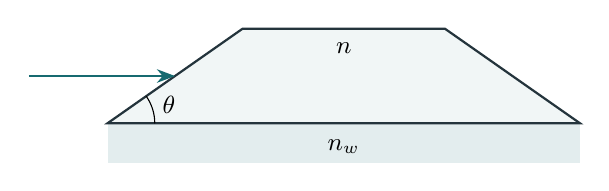
\begin{tikzpicture}[scale=1.0,font=\small]
\fill[accent!12](-3,-.5)rectangle(3,0);
\fill[accent!6](-3,0)--(3,0)--(1.28622239,1.20000000)--(-1.28622239,1.20000000)--cycle;
\draw[object](-3,0)--(3,0)--(1.28622239,1.20000000)--(-1.28622239,1.20000000)--cycle;
\draw[motion](-4,.6)--(-2.14311120,0.60000000);
\draw[thin](-2.4,0)arc(0:35:.6);
\node at(-2.22,.24){$\theta$};
\node at(0,.95){$n$};\node at(0,-.3){$n_w$};
\end{tikzpicture}
\figcaption{图光1.6\quad 截顶棱镜与浸水底面}
\end{minipage}\end{center}

\Needspace{6\baselineskip}\subsection*{解答}


解图光1.6A在L处从空气折入玻璃，在T处到达玻璃与水的底面，在R处从对称右斜面折回空气。图取35°工作角以清楚显示三段光路，所求最小角还须由临界条件计算。入口法线与水平线夹角$90^\circ-\theta$；设玻璃内折射角为$r$，则
\[
\cos\theta=n\sin r,\qquad
\sin r=\frac{\cos\theta}{n},\quad
\cos r=\frac{\sqrt{n^2-\cos^2\theta}}n.
\]
L处指向玻璃内部的法线向右下，与水平夹角为$90^\circ-\theta$。玻璃内光线比该法线向上偏$r$，故它向右下的俯角为$90^\circ-\theta-r$；T处法线竖直，入射方向的反向延长线与它的夹角正是$\theta+r$。由图中相邻法线的关系，底面的入射角为$i_b=\theta+r$。底面全反射要求
\[
n\sin(\theta+r)\ge n_w.
\]
\begin{center}\begin{minipage}{.98\linewidth}\centering
\begin{tikzpicture}[scale=1.0,font=\small]
\fill[accent!12](-3,-.5)rectangle(3,0);
\fill[accent!6](-3,0)--(3,0)--(1.28622239,1.20000000)--(-1.28622239,1.20000000)--cycle;
\draw[object](-3,0)--(3,0)--(1.28622239,1.20000000)--(-1.28622239,1.20000000)--cycle;
\draw[motion](-4,.6)--(-2.14311120,0.60000000);
\draw[thin](-2.4,0)arc(0:35:.6);
\node at(-2.22,.24){$\theta$};
\node at(0,.95){$n$};\node at(0,-.3){$n_w$};
\coordinate(L)at(-2.14311120,0.60000000);\coordinate(T)at(-0.65056739,0.00000000);\coordinate(R)at(1.66855924,0.93228485);
\draw[motion](L)--(T)--(R)--(4.00000000,0.93228485);
\draw[guide]($(L)+(125:.85)$)--($(L)+(-55:.85)$);
\draw[guide]($(T)+(0,-.4)$)--($(T)+(0,1.05)$);
\draw ($(L)+(125:.48)$)arc(125:180:.48);
\draw ($(L)+(-55:.55)$)arc(-55:-21.90004091:.55);
\draw ($(T)+(90:.55)$)arc(90:158.09995909:.55);
\node at(-2.80311120,0.96000000){$i_0$};
\node at(-1.57311120,0.16000000){$r$};
\node at(-1.13056739,0.72000000){$i_b$};
\node[above left]at(L){$L$};\node[below]at(T){$T$};\node[above left]at(R){$R$};
\node[align=left,anchor=west]at(4.6,.4){$\theta=35^\circ$的真实示例\\$i_0=55^\circ$\\$r=33.1000^\circ$\\$i_b=68.1000^\circ$\\临界角$i_c=62.4573^\circ$\\出射光仍平行于入射光\\L、T、R均为实际求得的交点};
\end{tikzpicture}
\figcaption{解图光1.6A\quad L处入口折射、T处底面反射与R处出射。图中取35°工作角，角度和三个交点均按折射定律计算}
\end{minipage}\end{center}
这里底面两侧介质是玻璃和水，临界角为$i_c=\arcsin(n_w/n)$；它与斜面的底角$\theta$不是同一个角。先将一般不等式写开，
\[
n\sin\theta\cos r+n\cos\theta\sin r\ge n_w,
\]
再分别代入入口所得的$\sin r,\cos r$，得到
\[
\sin\theta\sqrt{n^2-\cos^2\theta}+\cos^2\theta\ge n_w.
\]
在临界情形展开正弦，并代入$r$：
\[
\sin\theta\sqrt{n^2-\cos^2\theta}
+\cos^2\theta=n_w.
\]
把$\cos^2\theta$移到右边后，保留根式的不等式为
\[
\sqrt{1-\cos^2\theta}\sqrt{n^2-\cos^2\theta}
\ge n_w-\cos^2\theta.
\]
本题$n_w>1\ge\cos^2\theta$，移项后两边非负，允许平方。令$c=\cos^2\theta$，得到
\[
(1-c)(n^2-c)\ge(n_w-c)^2,
\]
\[
n^2-(n^2+1)c+c^2
\ge n_w^2-2n_wc+c^2.
\]
两边同有$c^2$，消去并把含$c$的项移到同一边，得
\[
(n^2-2n_w+1)c\le n^2-n_w^2.
\]
本题$n^2-2n_w+1=0.59>0$，所以除以该数时不等号方向保持。于是
\[
\boxed{\cos^2\theta\le
\frac{n^2-n_w^2}{n^2-2n_w+1}},\qquad
\boxed{\theta_{\min}\approx25.44^\circ}.
\]
代入数据时，分子为$2.25-1.7689=0.4811$，故$c\le0.4811/0.59=0.8154237288$，再依次开平方、取反余弦，得到$\theta_{\min}=25.443662933^\circ$，按一位小数为25.4°。临界处$r=37.013661912^\circ$，$i_b=62.457324846^\circ=i_c$，入口角由 $\cos\theta=n\sin r$ 给出，底面的临界条件在此取等号。

等号为临界掠射；要求严格全反射时取$\theta>\theta_{\min}$。上述角度条件针对落在底面、再从另一斜面出射的光线，截顶位置和入射高度须按图选择，不能仅凭角度不等式保证任意入射位置均走这条光路。
\begin{center}\begin{minipage}{.97\linewidth}\centering
\begin{tikzpicture}[x=.08cm,y=.045cm,font=\small]
\draw[axis](0,35)--(96,35)node[right]{$\theta/{}^\circ$};
\draw[axis](0,35)--(0,97)node[above]{$i_b/{}^\circ$};
\draw[guide](0,62.45732485)--(90,62.45732485);
\draw[guide](25.44366293,35)--(25.44366293,62.45732485);
\draw[traj]plot coordinates {(0.00000000,41.81031490) (0.50000000,42.30836360) (1.00000000,42.80251022) (1.50000000,43.29275627) (2.00000000,43.77910427) (2.50000000,44.26155775) (3.00000000,44.74012124) (3.50000000,45.21480026) (4.00000000,45.68560132) (4.50000000,46.15253191) (5.00000000,46.61560051) (5.50000000,47.07481654) (6.00000000,47.53019037) (6.50000000,47.98173331) (7.00000000,48.42945763) (7.50000000,48.87337645) (8.00000000,49.31350385) (8.50000000,49.74985473) (9.00000000,50.18244491) (9.50000000,50.61129102) (10.00000000,51.03641053) (10.50000000,51.45782170) (11.00000000,51.87554362) (11.50000000,52.28959611) (12.00000000,52.69999975) (12.50000000,53.10677584) (13.00000000,53.50994641) (13.50000000,53.90953413) (14.00000000,54.30556237) (14.50000000,54.69805509) (15.00000000,55.08703691) (15.50000000,55.47253300) (16.00000000,55.85456912) (16.50000000,56.23317156) (17.00000000,56.60836712) (17.50000000,56.98018311) (18.00000000,57.34864730) (18.50000000,57.71378789) (19.00000000,58.07563352) (19.50000000,58.43421323) (20.00000000,58.78955642) (20.50000000,59.14169284) (21.00000000,59.49065257) (21.50000000,59.83646601) (22.00000000,60.17916381) (22.50000000,60.51877691) (23.00000000,60.85533647) (23.50000000,61.18887387) (24.00000000,61.51942069) (24.50000000,61.84700867) (25.00000000,62.17166971) (25.50000000,62.49343586) (26.00000000,62.81233927) (26.50000000,63.12841219) (27.00000000,63.44168693) (27.50000000,63.75219590) (28.00000000,64.05997152) (28.50000000,64.36504624) (29.00000000,64.66745254) (29.50000000,64.96722287) (30.00000000,65.26438968) (30.50000000,65.55898538) (31.00000000,65.85104231) (31.50000000,66.14059278) (32.00000000,66.42766901) (32.50000000,66.71230312) (33.00000000,66.99452716) (33.50000000,67.27437304) (34.00000000,67.55187256) (34.50000000,67.82705740) (35.00000000,68.09995909) (35.50000000,68.37060900) (36.00000000,68.63903835) (36.50000000,68.90527819) (37.00000000,69.16935941) (37.50000000,69.43131269) (38.00000000,69.69116854) (38.50000000,69.94895726) (39.00000000,70.20470898) (39.50000000,70.45845359) (40.00000000,70.71022077) (40.50000000,70.96004000) (41.00000000,71.20794052) (41.50000000,71.45395137) (42.00000000,71.69810135) (42.50000000,71.94041900) (43.00000000,72.18093267) (43.50000000,72.41967044) (44.00000000,72.65666017) (44.50000000,72.89192947) (45.00000000,73.12550570) (45.50000000,73.35741599) (46.00000000,73.58768720) (46.50000000,73.81634598) (47.00000000,74.04341870) (47.50000000,74.26893149) (48.00000000,74.49291025) (48.50000000,74.71538060) (49.00000000,74.93636795) (49.50000000,75.15589743) (50.00000000,75.37399394) (50.50000000,75.59068214) (51.00000000,75.80598643) (51.50000000,76.01993098) (52.00000000,76.23253971) (52.50000000,76.44383630) (53.00000000,76.65384420) (53.50000000,76.86258662) (54.00000000,77.07008653) (54.50000000,77.27636666) (55.00000000,77.48144954) (55.50000000,77.68535743) (56.00000000,77.88811239) (56.50000000,78.08973626) (57.00000000,78.29025063) (57.50000000,78.48967692) (58.00000000,78.68803628) (58.50000000,78.88534969) (59.00000000,79.08163788) (59.50000000,79.27692142) (60.00000000,79.47122063) (60.50000000,79.66455566) (61.00000000,79.85694645) (61.50000000,80.04841274) (62.00000000,80.23897408) (62.50000000,80.42864983) (63.00000000,80.61745918) (63.50000000,80.80542112) (64.00000000,80.99255446) (64.50000000,81.17887784) (65.00000000,81.36440973) (65.50000000,81.54916842) (66.00000000,81.73317205) (66.50000000,81.91643858) (67.00000000,82.09898582) (67.50000000,82.28083142) (68.00000000,82.46199288) (68.50000000,82.64248756) (69.00000000,82.82233264) (69.50000000,83.00154520) (70.00000000,83.18014216) (70.50000000,83.35814030) (71.00000000,83.53555628) (71.50000000,83.71240662) (72.00000000,83.88870772) (72.50000000,84.06447586) (73.00000000,84.23972720) (73.50000000,84.41447778) (74.00000000,84.58874353) (74.50000000,84.76254028) (75.00000000,84.93588374) (75.50000000,85.10878953) (76.00000000,85.28127317) (76.50000000,85.45335007) (77.00000000,85.62503558) (77.50000000,85.79634493) (78.00000000,85.96729329) (78.50000000,86.13789572) (79.00000000,86.30816723) (79.50000000,86.47812273) (80.00000000,86.64777709) (80.50000000,86.81714508) (81.00000000,86.98624143) (81.50000000,87.15508078) (82.00000000,87.32367774) (82.50000000,87.49204685) (83.00000000,87.66020260) (83.50000000,87.82815944) (84.00000000,87.99593175) (84.50000000,88.16353390) (85.00000000,88.33098020) (85.50000000,88.49828494) (86.00000000,88.66546236) (86.50000000,88.83252668) (87.00000000,88.99949210) (87.50000000,89.16637278) (88.00000000,89.33318288) (88.50000000,89.49993653) (89.00000000,89.66664786) (89.50000000,89.83333098) (90.00000000,90.00000000)};
\fill[color=warm](25.44366293,62.45732485)circle(1.5pt);
\foreach \a in{0,30,60,90}{\node[below]at(\a,35){\a};}
\foreach \a in{45,60,75,90}{\node[left]at(0,\a){\a};}
\node[below,anchor=north west]at(25.44366293,28){$\theta_{\min}=25.4437^\circ$};
\node[align=left,anchor=west]at(107,73){$i_b=\theta+\arcsin(\cos\theta/n)$\\$i_c=62.4573^\circ$\\曲线严格上升\\临界交点右侧才满足角度条件\\另须检查实际光线落到底面};
\end{tikzpicture}
\figcaption{解图光1.6B　底面入射角随斜面底角严格增加，唯一交点给出临界值。临界角是纵坐标，所求底角是横坐标。}
\end{minipage}\end{center}

解图光1.6B还可检查这个根是不是最小值。由入口关系求导，
\[
\frac{di_b}{d\theta}
=1-\frac{\sin\theta}{\sqrt{n^2-\cos^2\theta}}>0
\qquad(0<\theta<\pi/2,\ n>1),
\]
因为根号内减去$\sin^2\theta$恰为$n^2-1>0$。所以$i_b$从$\arcsin(1/n)$严格增加到90°，只与本题的$i_c$相交一次，不存在另一支更小角度满足条件。对$1<n_w<n$，分母$n^2-2n_w+1>(n-1)^2>0$，上式的临界底角处于0与90°之间；$n_w=n$时只能达到掠射极限，$n_w>n$时不能产生这种全反射。

还可在A图逐个检查几何交点。取底面端点横坐标$\pm a$、截顶高度$h$、入口高度$y_L$，以底面为$y=0$，令$u=\tan(90^\circ-\theta-r)>0$，则
\[
x_L=-a+\frac{y_L}{\tan\theta},\qquad
x_T=x_L+\frac{y_L}{u},\qquad
y_R=\frac{u(a-x_T)}{1+u/\tan\theta},\qquad
x_R=a-\frac{y_R}{\tan\theta}.
\]
至少须有$0<h<a\tan\theta$、$0<y_L<h$、$-a<x_T<a$以及$0<y_R<h$，并检查途中不被截顶遮住。A图所用$a=3,h=1.2,y_L=0.6$给$x_T=-0.6505674,y_R=0.9322849$，各点均在所画面上。对称两斜面使出射相对法线角与入口相同，再由$n\sin r=\cos\theta$回到水平出射；全反射角条件本身不保证任意高度都有此通路。

\subsubsection*{像方向的转动}
第二问按维持三段通光的理想近轴视场讨论，在固定横向坐标中观察像的姿态；旋转时若实际开口或邻接介质改变，应另查通光条件。一次底面反射使横截面内一个方向翻转，另一个横向方向保留。解图光1.6C中以棱镜的反射翻转轴方向角为$\psi$，任一物体方向角$\chi$变成
\[
\chi'=2\psi-\chi.
\]
\begin{center}\begin{minipage}{.98\linewidth}\centering
\begin{tikzpicture}[scale=1.0,font=\small]
\begin{scope}[xshift=0.0cm]
\draw[guide](0,0)circle(1.7);\draw[guide](-1.9,0)--(1.9,0);
\draw[object](30:1.9)--(210:1.9);
\draw[motion](0,0)--(70:1.5);
\draw[force](0,0)--(-10:1.5);
\node[above left]at(70:1.85){$\chi=70^\circ$};
\node[below right]at(-10:1.65){$\chi^\prime=-10^\circ$};
\node[above right]at(30:1.95){$\psi=30^\circ$};
\node at(0,-2.3){$\psi=30^\circ,\quad\chi^\prime=-10^\circ$};
\end{scope}
\begin{scope}[xshift=6.5cm]
\draw[guide](0,0)circle(1.7);\draw[guide](-1.9,0)--(1.9,0);
\draw[object](50:1.9)--(230:1.9);
\draw[motion](0,0)--(70:1.5);
\draw[force](0,0)--(30:1.5);
\node[above left]at(70:1.85){$\chi=70^\circ$};
\node[below right]at(30:1.65){$\chi^\prime=30^\circ$};
\node[above right]at(50:1.95){$\psi=50^\circ$};
\node at(0,-2.3){$\psi=50^\circ,\quad\chi^\prime=30^\circ$};
\end{scope}
\node[align=center]at(3.25,-3.05){同一物方向不动，反射轴由30°转到50°\\像方向由$-10^\circ$转到$30^\circ$，增量为轴转角的两倍};
\end{tikzpicture}
\figcaption{解图光1.6C\quad 横向反射映射给像的两倍转角}
\end{minipage}\end{center}
解图光1.6C中的物箭头始终朝70°。反射轴从30°转到50°时，像箭头由$-10^\circ$变为30°，物、像相对轴分处两侧，角度相反。用横向方向单位矢量$\boldsymbol u=(\cos\chi,\sin\chi)$也能逐步写出此关系：先将坐标转到反射轴，再反射，最后转回固定坐标，
\[
\boldsymbol u'
=\mathsf R(\psi)
\begin{pmatrix}1&0\\0&-1\end{pmatrix}
\mathsf R(-\psi)\boldsymbol u
=
\begin{pmatrix}
\cos2\psi&\sin2\psi\\
\sin2\psi&-\cos2\psi
\end{pmatrix}\boldsymbol u.
\]
矩阵乘法给$\boldsymbol u'=(\cos(2\psi-\chi),\sin(2\psi-\chi))$，从而方向角满足上式。其行列式为$-1$，说明两倍转角仍伴有镜像翻转；不能把有方向的字母像说成经过一次反射后完全正立。

物体静止而棱镜转动时，$\dot\psi=\omega$，所以
\[
\boxed{\dot\chi'=2\omega}.
\]
像相对固定观察坐标转动的角速度是棱镜的两倍，且保留一次反射的横向镜像关系。棱镜旋转$180^\circ$，像转过$360^\circ$，恢复原有朝向；这描述的是像姿态的转动，不是把单根轴上光线的传播方向改成绕轴转动。

\Needspace{13\baselineskip}

\pdfbookmark[2]{第 7 题 跑道上方的梯度折射与可见距离}{q7}

\section*{第 7 题\quad 跑道上方的梯度折射与可见距离}\label{q:7}

机场跑道上方空气的折射率随高度$y$变化为
\[
n(y)=n_0(1+ay),\qquad a=1.5\times10^{-6}\,\mathrm{m}^{-1}.
\]
一人站在跑道上，眼睛距地面$h=1.7\,\mathrm m$。忽略地球曲率，求他能看到的跑道最远距离$d$。给出光线轨迹和采用的近似。

\begin{center}\begin{minipage}{.98\linewidth}\centering
\begin{tikzpicture}[scale=.9,transform shape]
\draw[axis] (0.00000,0.00000)--(6.00000,0.00000);\draw[axis] (0.00000,0.00000)--(0.00000,2.50000);\node[above] at (0.00000,2.50000) {$y$};\node[below] at (6.00000,0.00000) {跑道};\fill (5.00000,2.00000) circle(.035);\node[right] at (5.00000,2.00000) {$E$};\draw[<->,thin,color=muted] (5.45000,0.00000)--(5.45000,2.00000);\node[right] at (5.45000,1.00000) {$h$};\draw[<->,thin,color=muted] (0.00000,-0.50000)--(5.00000,-0.50000);\node[below] at (2.50000,-0.50000) {$d$};
\end{tikzpicture}
\figcaption{图光1.7\quad 眼高与最远可见地面点；水平距离与高度分别缩放}
\end{minipage}\end{center}

\Needspace{6\baselineskip}\subsection*{解答}


极限光线从跑道表面水平出发，随后因上方折射率较大而逐渐向上弯曲，恰好到达眼高$h$。来自更远地面的光线即使以最小向上角发射，到达观察者所在竖直平面时也会高于眼睛。解图光1.7A用这一极限光线限定可见距离。
\begin{center}\begin{minipage}{.98\linewidth}\centering
\begin{tikzpicture}[x=4.5cm,y=2.4cm,font=\small]
\draw[axis](0,0)--(1.26,0)node[right]{$x/d$};
\draw[axis](0,0)--(0,1.6)node[above]{$y/h$};
\draw[guide](0,1)--(1.15,1);\draw[guide](1,0)--(1,1);
\draw[motion]plot coordinates {(0.000000000,0.000000000) (0.010000000,0.000100000) (0.020000000,0.000400000) (0.030000000,0.000900000) (0.040000000,0.001599999) (0.050000000,0.002499999) (0.060000000,0.003599998) (0.070000000,0.004899998) (0.080000000,0.006399997) (0.090000000,0.008099997) (0.100000000,0.009999996) (0.110000000,0.012099995) (0.120000000,0.014399994) (0.130000000,0.016899993) (0.140000000,0.019599992) (0.150000000,0.022499991) (0.160000000,0.025599989) (0.170000000,0.028899988) (0.180000000,0.032399987) (0.190000000,0.036099985) (0.200000000,0.039999984) (0.210000000,0.044099982) (0.220000000,0.048399980) (0.230000000,0.052899979) (0.240000000,0.057599977) (0.250000000,0.062499975) (0.260000000,0.067599973) (0.270000000,0.072899971) (0.280000000,0.078399969) (0.290000000,0.084099967) (0.300000000,0.089999965) (0.310000000,0.096099963) (0.320000000,0.102399961) (0.330000000,0.108899959) (0.340000000,0.115599957) (0.350000000,0.122499954) (0.360000000,0.129599952) (0.370000000,0.136899950) (0.380000000,0.144399947) (0.390000000,0.152099945) (0.400000000,0.159999943) (0.410000000,0.168099941) (0.420000000,0.176399938) (0.430000000,0.184899936) (0.440000000,0.193599934) (0.450000000,0.202499931) (0.460000000,0.211599929) (0.470000000,0.220899927) (0.480000000,0.230399925) (0.490000000,0.240099922) (0.500000000,0.249999920) (0.510000000,0.260099918) (0.520000000,0.270399916) (0.530000000,0.280899914) (0.540000000,0.291599912) (0.550000000,0.302499910) (0.560000000,0.313599909) (0.570000000,0.324899907) (0.580000000,0.336399905) (0.590000000,0.348099904) (0.600000000,0.359999902) (0.610000000,0.372099901) (0.620000000,0.384399899) (0.630000000,0.396899898) (0.640000000,0.409599897) (0.650000000,0.422499896) (0.660000000,0.435599896) (0.670000000,0.448899895) (0.680000000,0.462399894) (0.690000000,0.476099894) (0.700000000,0.489999894) (0.710000000,0.504099894) (0.720000000,0.518399894) (0.730000000,0.532899894) (0.740000000,0.547599895) (0.750000000,0.562499895) (0.760000000,0.577599896) (0.770000000,0.592899897) (0.780000000,0.608399899) (0.790000000,0.624099900) (0.800000000,0.639999902) (0.810000000,0.656099904) (0.820000000,0.672399906) (0.830000000,0.688899909) (0.840000000,0.705599912) (0.850000000,0.722499915) (0.860000000,0.739599918) (0.870000000,0.756899922) (0.880000000,0.774399926) (0.890000000,0.792099930) (0.900000000,0.809999935) (0.910000000,0.828099940) (0.920000000,0.846399945) (0.930000000,0.864899950) (0.940000000,0.883599956) (0.950000000,0.902499963) (0.960000000,0.921599969) (0.970000000,0.940899976) (0.980000000,0.960399984) (0.990000000,0.980099992) (1.000000000,1.000000000)};
\draw[guide,color=warm]plot coordinates {(0.000000000,0.000000000) (0.009207008,0.006607860) (0.018414016,0.013385257) (0.027621024,0.020332193) (0.036828032,0.027448667) (0.046035040,0.034734679) (0.055242048,0.042190229) (0.064449056,0.049815317) (0.073656064,0.057609943) (0.082863072,0.065574107) (0.092070080,0.073707809) (0.101277089,0.082011049) (0.110484097,0.090483828) (0.119691105,0.099126144) (0.128898113,0.107937998) (0.138105121,0.116919391) (0.147312129,0.126070321) (0.156519137,0.135390790) (0.165726145,0.144880797) (0.174933153,0.154540342) (0.184140161,0.164369425) (0.193347169,0.174368046) (0.202554177,0.184536205) (0.211761185,0.194873902) (0.220968193,0.205381137) (0.230175201,0.216057911) (0.239382209,0.226904222) (0.248589217,0.237920072) (0.257796225,0.249105460) (0.267003233,0.260460386) (0.276210241,0.271984850) (0.285417249,0.283678853) (0.294624257,0.295542393) (0.303831266,0.307575472) (0.313038274,0.319778088) (0.322245282,0.332150243) (0.331452290,0.344691936) (0.340659298,0.357403168) (0.349866306,0.370283937) (0.359073314,0.383334245) (0.368280322,0.396554091) (0.377487330,0.409943475) (0.386694338,0.423502397) (0.395901346,0.437230858) (0.405108354,0.451128856) (0.414315362,0.465196393) (0.423522370,0.479433469) (0.432729378,0.493840082) (0.441936386,0.508416234) (0.451143394,0.523161923) (0.460350402,0.538077152) (0.469557410,0.553161918) (0.478764418,0.568416223) (0.487971426,0.583840066) (0.497178434,0.599433447) (0.506385443,0.615196367) (0.515592451,0.631128824) (0.524799459,0.647230821) (0.534006467,0.663502355) (0.543213475,0.679943428) (0.552420483,0.696554039) (0.561627491,0.713334188) (0.570834499,0.730283876) (0.580041507,0.747403102) (0.589248515,0.764691867) (0.598455523,0.782150170) (0.607662531,0.799778011) (0.616869539,0.817575390) (0.626076547,0.835542308) (0.635283555,0.853678765) (0.644490563,0.871984759) (0.653697571,0.890460293) (0.662904579,0.909105364) (0.672111587,0.927919974) (0.681318595,0.946904123) (0.690525603,0.966057810) (0.699732612,0.985381035) (0.708939620,1.004873799) (0.718146628,1.024536101) (0.727353636,1.044367942) (0.736560644,1.064369321) (0.745767652,1.084540238) (0.754974660,1.104880695) (0.764181668,1.125390689) (0.773388676,1.146070223) (0.782595684,1.166919294) (0.791802692,1.187937905) (0.801009700,1.209126053) (0.810216708,1.230483741) (0.819423716,1.252010967) (0.828630724,1.273707731) (0.837837732,1.295574034) (0.847044740,1.317609876) (0.856251748,1.339815256) (0.865458756,1.362190175) (0.874665764,1.384734633) (0.883872772,1.407448629) (0.893079780,1.430332164) (0.902286789,1.453385237) (0.911493797,1.476607849) (0.920700805,1.500000000)};
\fill(0,0)circle(1.2pt);\node[below left]at(0,0){$O$};
\fill(1,1)circle(1.2pt);\node[above right]at(1,1){$E$};
\node[below]at(1,0){1};\node[left]at(0,1){1};
\node[align=left,anchor=west]at(1.48,.9){实线：水平出射$\eta_0=0$\\虚线：$\eta_0=0.8\,{\rm mrad}$\\两条均按给定折射率精确计算\\E的实际坐标为$(d,h)$\\横、纵各自缩放，不能据图量角\\较大初始仰角在同距处更高};
\end{tikzpicture}
\figcaption{解图光1.7A\quad 给定参数下的真实光线轨迹；横、纵各以$d$和$h$归一，较大初始仰角在同一水平距离处更高}
\end{minipage}\end{center}
把空气分成水平薄层，设光线与竖直法线的夹角为$\theta$。相邻水平薄层有共同的竖直法线，逐层折射定律给
\[
n_0=n_1\sin\theta_1=n_2\sin\theta_2=\cdots=n(y)\sin\theta.
\]
入口沿地面水平出射，与各层的竖直法线成 $\theta_0=90^\circ$，所以守恒量为 $n_0\sin90^\circ=n_0$。由各层折射定律，
\[
n(y)\sin\theta=n_0,
\qquad
\sin\theta=\frac1{1+ay}.
\]
\begin{center}\begin{minipage}{.97\linewidth}\centering
\begin{tikzpicture}[x=2.0cm,y=1.8cm,font=\small]
\draw[axis](0,0)--(2.65,0)node[right]{$\eta/{\rm mrad}$};
\draw[axis](0,0)--(0,1.95)node[above]{$y/{\rm m}$};
\draw[guide](0,1.7)--(2.258315559,1.7)--(2.258315559,0);
\draw[traj]plot coordinates {(0.000000000,0.000000000) (0.225831793,0.017000000) (0.319374382,0.034000000) (0.391152132,0.051000000) (0.451663572,0.068000000) (0.504975220,0.085000000) (0.553172632,0.102000000) (0.597494725,0.119000000) (0.638748723,0.136000000) (0.677495323,0.153000000) (0.714142767,0.170000000) (0.748999245,0.187000000) (0.782304189,0.204000000) (0.814248007,0.221000000) (0.844985081,0.238000000) (0.874642645,0.255000000) (0.903327030,0.272000000) (0.931128180,0.289000000) (0.958122982,0.306000000) (0.984377777,0.323000000) (1.009950279,0.340000000) (1.034891068,0.357000000) (1.059244767,0.374000000) (1.083050981,0.391000000) (1.106345053,0.408000000) (1.129158679,0.425000000) (1.151520416,0.442000000) (1.173456096,0.459000000) (1.194989184,0.476000000) (1.216141064,0.493000000) (1.236931293,0.510000000) (1.257377811,0.527000000) (1.277497119,0.544000000) (1.297304444,0.561000000) (1.316813862,0.578000000) (1.336038425,0.595000000) (1.354990257,0.612000000) (1.373680646,0.629000000) (1.392120122,0.646000000) (1.410318528,0.663000000) (1.428285079,0.680000000) (1.446028415,0.697000000) (1.463556657,0.714000000) (1.480877441,0.731000000) (1.497997965,0.748000000) (1.514925016,0.765000000) (1.531665011,0.782000000) (1.548224017,0.799000000) (1.564607779,0.816000000) (1.580821748,0.833000000) (1.596871094,0.850000000) (1.612760733,0.867000000) (1.628495339,0.884000000) (1.644079364,0.901000000) (1.659517050,0.918000000) (1.674812444,0.935000000) (1.689969408,0.952000000) (1.704991636,0.969000000) (1.719882657,0.986000000) (1.734645851,1.003000000) (1.749284453,1.020000000) (1.763801567,1.037000000) (1.778200167,1.054000000) (1.792483110,1.071000000) (1.806653138,1.088000000) (1.820712888,1.105000000) (1.834664896,1.122000000) (1.848511600,1.139000000) (1.862255350,1.156000000) (1.875898409,1.173000000) (1.889442957,1.190000000) (1.902891100,1.207000000) (1.916244865,1.224000000) (1.929506213,1.241000000) (1.942677036,1.258000000) (1.955759163,1.275000000) (1.968754363,1.292000000) (1.981664345,1.309000000) (1.994490764,1.326000000) (2.007235222,1.343000000) (2.019899271,1.360000000) (2.032484413,1.377000000) (2.044992106,1.394000000) (2.057423761,1.411000000) (2.069780750,1.428000000) (2.082064401,1.445000000) (2.094276005,1.462000000) (2.106416815,1.479000000) (2.118488048,1.496000000) (2.130490886,1.513000000) (2.142426480,1.530000000) (2.154295947,1.547000000) (2.166100373,1.564000000) (2.177840818,1.581000000) (2.189518309,1.598000000) (2.201133849,1.615000000) (2.212688413,1.632000000) (2.224182952,1.649000000) (2.235618391,1.666000000) (2.246995634,1.683000000) (2.258315559,1.700000000)};
\foreach \a in{0,1,2}{\node[below]at(\a,0){\a};}
\node[left]at(0,1.7){1.7};
\node[align=left,anchor=west]at(3.3,1.0){$\eta$从水平量，$\theta$从竖直量\\$\eta+\theta=90^\circ$\\$\cos\eta=1/(1+ay)$\\眼高处$\eta=2.258316\,{\rm mrad}$\\即约$0.1294^\circ$\\$n\sin\theta=n\cos\eta=n_0$};
\end{tikzpicture}
\figcaption{解图光1.7B　水平仰角随高度的实际变化。竖直法线角$\theta$是其余角，眼高处仰角仅约2.26毫弧度。}
\end{minipage}\end{center}

解图光1.7B 的仰角 $\eta$ 从水平方向量起，与从竖直法线量起的 $\theta$ 互余，故层间守恒量也可写成 $n\cos\eta$。在折射率较大的高处，$\cos\eta$ 变小、仰角增大，光线逐渐向上弯曲。轨迹斜率与角度关系为
\[
\frac{\dd y}{\dd x}=\cot\theta,\qquad
1+\left(\frac{\dd y}{\dd x}\right)^2
=\frac1{\sin^2\theta}=(1+ay)^2.
\]
在厚度为$\dd y$的薄层中，水平位移为$\dd x$，光线对竖直法线的正切是$\dd x/\dd y$，故$\dd y/\dd x=\cot\theta$。也可直接写
\[
\sin\theta=\frac1{\sqrt{1+\cot^2\theta}}
=\frac1{\sqrt{1+(y')^2}}.
\]
取向上弯曲的正斜率支，
\[
y'=\sqrt{(1+ay)^2-1}.
\]
保留折射率平方中的二次项，先解给定模型的完整方程。令$u=1+ay$，分离变量：
\[
\frac{\dd u}{\sqrt{u^2-1}}=a\,\dd x,\qquad
\operatorname{arcosh}(1+ay)=ax,
\]
利用$y(0)=0$得到
\[
\boxed{y(x)=\frac{\cosh(ax)-1}{a}},\qquad
\boxed{d=\frac{\operatorname{arcosh}(1+ah)}a}.
\]
在$y'=0$的初始点，正平方根的一阶方程须与平滑介质中的射线方程相容。由费马方程
\[
\frac{\dd}{\dd x}
\left(\frac{n(y)y'}{\sqrt{1+(y')^2}}\right)
=n_y(y)\sqrt{1+(y')^2}
\]
得到$y''=n_y(1+(y')^2)/n$。代入本题守恒量即为$y''=a(1+ay)$，初值$y(0)=y'(0)=0$唯一确定上面的双曲余弦解，而且$y''(0)=a>0$。光线在地面处已经有正曲率，从出发点起就向上弯。

由于$ah=2.55\times10^{-6}\ll1$，$\cosh(ax)=1+(ax)^2/2+\cdots$，也可直接从斜率方程作同一近似。平方项展开为
\[
1+(y')^2=1+2ay+a^2y^2.
\]
在$0\le y\le h$，所舍的$a^2y^2$相对保留项$2ay$的比值不超过$ah/2=1.275\times10^{-6}$，故
\[
y'\simeq\sqrt{2ay},\qquad
\frac{\dd y}{\sqrt y}=\sqrt{2a}\,\dd x,\qquad
2\sqrt y=\sqrt{2a}\,x+C.
\]
$y(0)=0$给$C=0$，取向上出射的正支后，得到
\[
y\simeq\frac a2x^2,\qquad
\boxed{d\simeq\sqrt{\frac{2h}{a}}
=1.506\times10^3\,\mathrm m}.
\]
展开精确距离还可得
\[
d=\sqrt{\frac{2h}{a}}
\left(1-\frac{ah}{12}+O((ah)^2)\right).
\]
将$d=2\operatorname{arsinh}\sqrt{ah/2}/a$代入题给数据，精确轨迹给$d=1505.544985\,\mathrm{m}$，抛物线近似给$d=1505.545305\,\mathrm{m}$，后者大约偏大$0.32\,\mathrm{mm}$。相对修正约$2.125\times10^{-7}$，远小于题给数据的精度；列出这些位数是为了看出两个模型的差值。图中光线在连续的折射率梯度中逐渐弯曲，计算采用眼高范围内的线性折射率分布。\begin{center}\begin{minipage}{.97\linewidth}\centering
\begin{tikzpicture}[x=.8cm,y=3.0cm,font=\small]
\draw[axis](0,0)--(6.6,0)node[right]{$\eta_0/{\rm mrad}$};
\draw[axis](0,0)--(0,1.17)node[above]{$d(\eta_0)/d(0)$};
\draw[guide](0,1)--(6,1);\draw[traj]plot coordinates {(0.000000000,1.000000000) (0.050000000,0.978104690) (0.100000000,0.956699156) (0.150000000,0.935782318) (0.200000000,0.915352391) (0.250000000,0.895406892) (0.300000000,0.875942658) (0.350000000,0.856955872) (0.400000000,0.838442085) (0.450000000,0.820396251) (0.500000000,0.802812757) (0.550000000,0.785685464) (0.600000000,0.769007739) (0.650000000,0.752772502) (0.700000000,0.736972268) (0.750000000,0.721599182) (0.800000000,0.706645072) (0.850000000,0.692101483) (0.900000000,0.677959725) (0.950000000,0.664210910) (1.000000000,0.650845992) (1.050000000,0.637855807) (1.100000000,0.625231107) (1.150000000,0.612962595) (1.200000000,0.601040956) (1.250000000,0.589456885) (1.300000000,0.578201119) (1.350000000,0.567264455) (1.400000000,0.556637777) (1.450000000,0.546312077) (1.500000000,0.536278467) (1.550000000,0.526528200) (1.600000000,0.517052684) (1.650000000,0.507843488) (1.700000000,0.498892360) (1.750000000,0.490191227) (1.800000000,0.481732208) (1.850000000,0.473507616) (1.900000000,0.465509961) (1.950000000,0.457731956) (2.000000000,0.450166516) (2.050000000,0.442806759) (2.100000000,0.435646007) (2.150000000,0.428677781) (2.200000000,0.421895806) (2.250000000,0.415294002) (2.300000000,0.408866484) (2.350000000,0.402607561) (2.400000000,0.396511727) (2.450000000,0.390573661) (2.500000000,0.384788225) (2.550000000,0.379150452) (2.600000000,0.373655548) (2.650000000,0.368298887) (2.700000000,0.363076002) (2.750000000,0.357982584) (2.800000000,0.353014478) (2.850000000,0.348167673) (2.900000000,0.343438302) (2.950000000,0.338822638) (3.000000000,0.334317086) (3.050000000,0.329918177) (3.100000000,0.325622571) (3.150000000,0.321427045) (3.200000000,0.317328493) (3.250000000,0.313323920) (3.300000000,0.309410437) (3.350000000,0.305585260) (3.400000000,0.301845706) (3.450000000,0.298189185) (3.500000000,0.294613202) (3.550000000,0.291115348) (3.600000000,0.287693301) (3.650000000,0.284344822) (3.700000000,0.281067751) (3.750000000,0.277860001) (3.800000000,0.274719563) (3.850000000,0.271644493) (3.900000000,0.268632920) (3.950000000,0.265683035) (4.000000000,0.262793091) (4.050000000,0.259961402) (4.100000000,0.257186341) (4.150000000,0.254466335) (4.200000000,0.251799865) (4.250000000,0.249185463) (4.300000000,0.246621712) (4.350000000,0.244107240) (4.400000000,0.241640722) (4.450000000,0.239220879) (4.500000000,0.236846471) (4.550000000,0.234516300) (4.600000000,0.232229208) (4.650000000,0.229984074) (4.700000000,0.227779814) (4.750000000,0.225615377) (4.800000000,0.223489748) (4.850000000,0.221401943) (4.900000000,0.219351009) (4.950000000,0.217336026) (5.000000000,0.215356098) (5.050000000,0.213410360) (5.100000000,0.211497974) (5.150000000,0.209618127) (5.200000000,0.207770031) (5.250000000,0.205952923) (5.300000000,0.204166061) (5.350000000,0.202408727) (5.400000000,0.200680225) (5.450000000,0.198979880) (5.500000000,0.197307034) (5.550000000,0.195661052) (5.600000000,0.194041316) (5.650000000,0.192447226) (5.700000000,0.190878201) (5.750000000,0.189333674) (5.800000000,0.187813096) (5.850000000,0.186315934) (5.900000000,0.184841670) (5.950000000,0.183389799) (6.000000000,0.181959832)};
\foreach \a in{0,2,4,6}{\node[below]at(\a,0){\a};}
\node[left]at(0,1){1};
\node[align=left,anchor=west]at(8.1,.72){水平出射取得最大值$d(0)$\\$\eta_0$增大，可达水平距离减小\\$\eta_0=0:\quad d=1505.545\,{\rm m}$\\$\eta_0=0.8\,{\rm mrad}:\quad d=1063.886\,{\rm m}$\\$\eta_0=2\,{\rm mrad}:\quad d=677.746\,{\rm m}$\\只计从地面向上、连续到达眼高的光路};
\end{tikzpicture}
\figcaption{解图光1.7C　按同一折射率计算，不同初始仰角到达眼高的水平距离。曲线随仰角下降，水平出射决定可见边界。}
\end{minipage}\end{center}

\subsubsection*{为什么这条光线给最远距离}
解图光1.7C比较各个初始仰角的地面光线。设从地面向上发射的初始仰角为$0\le\eta_0<\pi/2$，令$b=\cos\eta_0$；守恒量改为$n_0b$，于是
\[
n(y)\cos\eta=n_0b,\qquad
\frac{\dd x}{\dd y}
=\frac{b}{\sqrt{(1+ay)^2-b^2}}.
\]
从地面到眼高的水平距离为
\[
d(\eta_0)=\int_0^h
\frac{b\,\dd y}{\sqrt{(1+ay)^2-b^2}}
=\frac b a\left[
\operatorname{arcosh}\frac{1+ah}{b}
-\operatorname{arcosh}\frac1b\right].
\]
对每个$y>0$，令$A=1+ay>1$，被积函数对$b$的导数为
\[
\frac{\partial}{\partial b}
\frac{b}{\sqrt{A^2-b^2}}
=\frac{A^2}{(A^2-b^2)^{3/2}}>0.
\]
故$b$越大距离越大，最大值取$b=1$，即$\eta_0=0$，回到前面的d。水平支在地面端的根式奇性可积，不导致距离发散；竖直出射极限$b\to0$则给水平距离0。对于固定眼位，比d更远的跑道点没有向上出射、连续到达眼高的光路；向下发射会先进入地面，不在本题模型内。以上比较只涉及$0\le y\le h$的折射率，地球曲率已按题设忽略。


\Needspace{13\baselineskip}

\pdfbookmark[2]{第 8 题 变折射率平板中的圆弧光路}{q8}

\section*{第 8 题\quad 变折射率平板中的圆弧光路}\label{q:8}

平板玻璃中折射率随水平坐标$x$变化：
\[
n(x)=\frac{n_0}{1-x/r},\qquad n_0=1.2,\quad r=13\,\mathrm{cm}.
\]
光线在$(0,0)$处沿$+y$轴进入玻璃，从上表面的$A$点进入空气，与上表面外法线成$\alpha=30^\circ$。求玻璃内光线轨迹、$A$点折射率和板厚$d$，取$0\le x<r$的光路。

\begin{center}\begin{minipage}{.98\linewidth}\centering
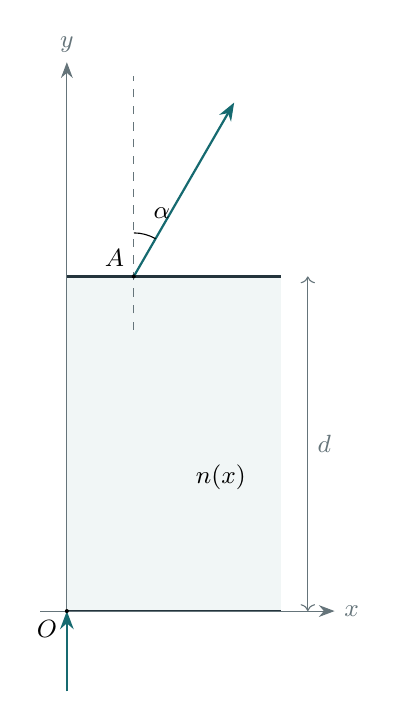
\begin{tikzpicture}[scale=.85,font=\small]
\fill[accent!6](0,0)rectangle(3.2,5);
\draw[object](0,0)--(3.2,0);\draw[object](0,5)--(3.2,5);
\draw[axis](-.4,0)--(4,0)node[right]{$x$};
\draw[axis](0,-.6)--(0,8.2)node[above]{$y$};
\draw[motion](0,-1.2)--(0,0);
\draw[guide](1,4.2)--(1,8.0);
\draw[motion](1,5)--(2.5,7.598076211);
\draw($(1,5)+(60:.65)$)arc(60:90:.65);
\node at(1.42,5.95){$\alpha$};
\fill(0,0)circle(.03);\node[below left]at(0,0){$O$};
\fill(1,5)circle(.03);\node[above left]at(1,5){$A$};
\node at(2.3,2){$n(x)$};
\draw[<->,color=muted](3.6,0)--(3.6,5)node[midway,right]{$d$};
\end{tikzpicture}
\figcaption{图光1.8\quad 随横坐标变化的介质与上表面出口}
\end{minipage}\end{center}

\Needspace{6\baselineskip}\subsection*{解答}


平板的出入口为水平面，折射率随水平坐标$x$变化。解图光1.8A把介质分成竖直薄层，层间法线沿$x$轴；设光线与$x$轴夹角为$\theta$，则
\[
n(x)\sin\theta=n_0,
\qquad
\sin\theta=1-\frac xr.
\]
竖直薄层的两面在不同x处，法线都平行于x轴，故层间关系可逐次写为
\[
n_0=n_1\sin\theta_1=n_2\sin\theta_2=\cdots=n(x)\sin\theta.
\]
进入点的$\theta=90^\circ$，故光线从竖直方向开始，逐渐向折射率较高的右方弯曲。
\begin{center}\begin{minipage}{.98\linewidth}\centering
\begin{tikzpicture}[scale=.68,font=\small]
\fill[accent!6](0,0)rectangle(3.2,5);
\draw[object](0,0)--(3.2,0);\draw[object](0,5)--(3.2,5);
\draw[axis](-.5,0)--(14.3,0)node[right]{$x/{\rm cm}$};
\draw[axis](0,-.8)--(0,8.2)node[above]{$y/{\rm cm}$};
\draw[motion](0,-1.2)--(0,0);
\draw[traj]plot coordinates {(0.000000000,0.000000000) (0.000101309,0.051322712) (0.000405234,0.102644625) (0.000911771,0.153964937) (0.001620911,0.205282850) (0.002532643,0.256597563) (0.003646954,0.307908277) (0.004963826,0.359214192) (0.006483238,0.410514508) (0.008205167,0.461808426) (0.010129586,0.513095146) (0.012256465,0.564373869) (0.014585770,0.615643796) (0.017117466,0.666904128) (0.019851513,0.718154065) (0.022787868,0.769392808) (0.025926486,0.820619561) (0.029267318,0.871833523) (0.032810311,0.923033896) (0.036555411,0.974219883) (0.040502558,1.025390686) (0.044651692,1.076545508) (0.049002748,1.127683550) (0.053555658,1.178804016) (0.058310351,1.229906109) (0.063266753,1.280989034) (0.068424787,1.332051992) (0.073784372,1.383094189) (0.079345425,1.434114830) (0.085107859,1.485113118) (0.091071584,1.536088260) (0.097236507,1.587039460) (0.103602533,1.637965924) (0.110169562,1.688866859) (0.116937491,1.739741471) (0.123906216,1.790588968) (0.131075627,1.841408557) (0.138445613,1.892199445) (0.146016059,1.942960842) (0.153786847,1.993691956) (0.161757855,2.044391996) (0.169928961,2.095060173) (0.178300035,2.145695695) (0.186870949,2.196297775) (0.195641567,2.246865624) (0.204611755,2.297398453) (0.213781371,2.347895474) (0.223150272,2.398355902) (0.232718314,2.448778949) (0.242485346,2.499163829) (0.252451216,2.549509757) (0.262615770,2.599815948) (0.272978848,2.650081619) (0.283540289,2.700305986) (0.294299929,2.750488266) (0.305257599,2.800627676) (0.316413130,2.850723437) (0.327766347,2.900774766) (0.339317073,2.950780883) (0.351065128,3.000741010) (0.363010329,3.050654367) (0.375152491,3.100520177) (0.387491422,3.150337662) (0.400026933,3.200106045) (0.412758826,3.249824553) (0.425686903,3.299492408) (0.438810964,3.349108838) (0.452130803,3.398673068) (0.465646213,3.448184327) (0.479356984,3.497641842) (0.493262900,3.547044844) (0.507363747,3.596392561) (0.521659304,3.645684224) (0.536149347,3.694919067) (0.550833653,3.744096320) (0.565711990,3.793215218) (0.580784128,3.842274995) (0.596049832,3.891274886) (0.611508864,3.940214128) (0.627160982,3.989091957) (0.643005944,4.037907613) (0.659043501,4.086660334) (0.675273404,4.135349361) (0.691695400,4.183973934) (0.708309233,4.232533296) (0.725114645,4.281026689) (0.742111372,4.329453358) (0.759299151,4.377812549) (0.776677713,4.426103507) (0.794246787,4.474325480) (0.812006100,4.522477716) (0.829955375,4.570559465) (0.848094332,4.618569978) (0.866422689,4.666508505) (0.884940159,4.714374300) (0.903646454,4.762166617) (0.922541283,4.809884711) (0.941624351,4.857527839) (0.960895360,4.905095257) (0.980354011,4.952586224) (1.000000000,5.000000000)};
\draw[motion](1,5)--(2.5,7.598076211);
\draw[guide](1,4.3)--(1,8.0);
\draw[guide](13,0)--(1,5);
\draw[guide](13,0)--(0,0);
\fill(0,0)circle(.035);\fill(1,5)circle(.035);\fill(13,0)circle(.035);
\node[below left]at(0,0){$O$};\node[above left]at(1,5){$A$};
\node[below]at(13,0){$C=(13,0)$};
\node[below]at(7.3,1.9){$CA=r$};
\draw[<->,color=muted](3.6,0)--(3.6,5)node[midway,right]{$d$};
\draw[<->,color=muted](0,-.9)--(1,-.9)node[midway,below]{$x_A$};
\node at(2.8,6.5){$\alpha=30^\circ$};
\node[align=left,anchor=west]at(6.6,5.6){$O=(0,0)$，$A=(1,5)\,{\rm cm}$\\$C=(13,0)\,{\rm cm}$在玻璃区域外\\光线只走O到A的圆弧\\$0\le x\le1<13,\quad0\le y\le5$\\半径CA垂直于A处内部切线\\坐标横纵按同一比例绘制};
\end{tikzpicture}
\figcaption{解图光1.8A\quad 按实际坐标绘制O到A的光线圆弧，C为辅助圆心；实际出射线与上表面法线成30°}
\end{minipage}\end{center}
在向右、向上传播的分支上，
\[
\frac{\dd y}{\dd x}=\tan\theta
=\frac{1-x/r}{\sqrt{1-(1-x/r)^2}}.
\]
令$u=1-x/r$，$\dd x=-r\,\dd u$。从$(0,0)$积分至$(x,y)$：
\[
y=-r\int_1^{\,1-x/r}\frac{u\,\dd u}{\sqrt{1-u^2}}
=r\sqrt{1-(1-x/r)^2}.
\]
令$u=1-x/r$，有$\dd\sqrt{1-u^2}=-u\,\dd u/\sqrt{1-u^2}$，恰与$\dd x=-r\,\dd u$中的负号相消。积分时$u$由$1$减至$1-x/r$，代入后得到向上传播对应的正高度$y$。再平方展开，
\[
y^2=r^2\left(1-1+\frac{2x}{r}-\frac{x^2}{r^2}\right)
=2rx-x^2=-(x-r)^2+r^2.
\]
因此
\[
\boxed{(x-r)^2+y^2=r^2,\quad x\ge0,\ y\ge0}.
\]
解图光1.8A 中，光线沿 $O\to A$ 向右上方前进，坐标满足 $0\le x\le x_A<r$、$0\le y\le d$。辅助半径 $CA$ 垂直于入射到上表面的切线。入口的 $y'(0^+)$ 趋于正无穷；若改用 $y$ 作自变量，入口切线可直接由
\[
x(y)=r-\sqrt{r^2-y^2},\qquad
x'(0)=0
\]
给出。由 $x'(0)=0$ 可知，入口处随 $y$ 增长的横向位移从二阶开始，光线沿 $+y$ 进入。
\subsubsection*{出口折射}
解图光1.8B中的$\theta_A$仍相对于水平线，而上表面法线竖直，所以出口入射角是$90^\circ-\theta_A$。两条关系分别为
\[
n_A\sin\theta_A=n_0,\qquad
n_A\cos\theta_A=\sin\alpha.
\]
\begin{center}\begin{minipage}{.98\linewidth}\centering
\begin{tikzpicture}[scale=1.0,font=\small]
\fill[accent!6](-2,-2.4)rectangle(2,0);
\draw[object](-2,0)--(2.2,0);
\draw[guide](0,-2.5)--(0,2.4);
\draw[motion](-.833333333,-2)--(0,0)--(1.2,2.078460969);
\draw[guide](-1.3,-.9)--(.8,-.9);
\draw($(0,0)+(180:.55)$)arc(180:247.38013505:.55);
\draw($(0,0)+(247.38013505:.88)$)arc(247.38013505:270:.88);
\draw($(0,0)+(60:.7)$)arc(60:90:.7);
\node at(-.62,-.48){$\theta_A$};
\node at(-.21,-1.2){$i_A$};
\node at(.4,.95){$\alpha$};
\node[below right]at(0,0){$A$};
\node at(1.15,-1.55){$n_A$};
\node[align=left,anchor=west]at(3.2,.1){分层法线水平，角为$\theta_A$\\上表面法线竖直，角为$i_A$\\$i_A+\theta_A=90^\circ$\\$\theta_A=67.3801^\circ$\\$i_A=22.6199^\circ$\\$n_A\sin i_A=\sin30^\circ=0.5$\\入射与出射均按实际角度画出};
\end{tikzpicture}
\figcaption{解图光1.8B\quad 出口局部的两条法线和互余角。内部入射方向为$5:12$，外部出射角为30°}
\end{minipage}\end{center}
也可不先平方相加，而把出口式逐项写成分式消角链，作为独立计算：
\[
\begin{aligned}
n_A&=\frac{\sin\alpha}{\cos\theta_A}
=\frac{\sin\alpha}{\sqrt{1-\sin^2\theta_A}}\\
&=\frac{\sin\alpha}{\sqrt{1-(n_0/n_A)^2}}
=\frac{n_A\sin\alpha}{\sqrt{n_A^2-n_0^2}}.
\end{aligned}
\]
所取角在第一象限，$n_A>0$，故可约去两端的$n_A$，得到$\sqrt{n_A^2-n_0^2}=\sin\alpha$，再平方求出同一结果。解图光1.8C将这两个分量放进直角三角形，平方相加消去$\theta_A$：
\[
\boxed{n_A=\sqrt{n_0^2+\sin^2\alpha}
=\sqrt{1.44+0.25}=1.3}.
\]
\begin{center}\begin{minipage}{.97\linewidth}\centering
\begin{tikzpicture}[x=3.2cm,y=3.2cm,font=\small]
\coordinate(O)at(0,0);\coordinate(H)at(.5,0);\coordinate(V)at(.5,1.2);
\draw[guide](O)--(H)--(V);
\draw[traj](0,0)--(.5,1.2);
\pic[draw,angle radius=2.5mm]{right angle=O--H--V};
\node[below]at(.25,0){$n_A\cos\theta_A=\sin\alpha=0.5$};
\node[right]at(.5,.6){$n_A\sin\theta_A=n_0=1.2$};
\node[left]at(.18,.65){$n_A=1.3$};
\node[align=left,anchor=west]at(2.2,.72){斜边为光学方向矢量的模长$n_A$\\水平分量由上表面折射确定\\竖直分量由层间守恒确定\\$n_A^2=n_0^2+\sin^2\alpha$\\本题分量比为$5:12$，斜边为13};
\end{tikzpicture}
\figcaption{解图光1.8C　层间守恒给竖直分量，上表面折射给水平分量；两个正分量平方相加得到出口折射率。}
\end{minipage}\end{center}

解图光1.8C 中，内部传播方向的单位向量乘 $n_A$ 后，竖直、水平分量分别为 $1.2$ 和 $0.5$，模长为 $1.3$。将两分量除以 $n_A$ 就得到 B 图内部入射方向的正弦与余弦，分别为 $\sin\theta_A=12/13$、$\cos\theta_A=5/13$。于是
\[
1-\frac{x_A}{r}=\frac{n_0}{n_A}=\frac{12}{13},
\qquad \boxed{x_A=1\,\mathrm{cm}}.
\]
把它代入已选取的上半圆弧，
\[
\boxed{d=y_A=\sqrt{2rx_A-x_A^2}
=\sqrt{26-1}\,\mathrm{cm}=5\,\mathrm{cm}}.
\]
出口的法向分量满足$n_A\cos\theta_A=0.5<1$，所以本题确有透射，不会在上表面全反射；所求位置也满足$x_A<r$，没有触及折射率模型的奇点。

\subsubsection*{一般出口角与透射范围}
保留$\alpha$不代数值，A、B、C图给出的一般关系为
\[
n_A=\sqrt{n_0^2+\sin^2\alpha},\qquad
x_A=r\left(1-\frac{n_0}{n_A}\right),\qquad
d=\frac{r\sin\alpha}{n_A}.
\]
也可从给定厚度反推出口角。用圆弧正支及$n(x_A)$，有
\[
r-x_A=\sqrt{r^2-d^2},\qquad
n_A=\frac{n_0r}{\sqrt{r^2-d^2}},\qquad
\sin\alpha=\frac{n_0d}{\sqrt{r^2-d^2}}.
\]
因此正常出射还要求$0<d<r/\sqrt{n_0^2+1}$。取等号时，光在空气中沿界面掠射；厚度再增大，上表面发生全反射，出射角方程失去实数解。本题$d=5\,\mathrm{cm}$小于临界厚度约$8.3224\,\mathrm{cm}$，而且$x_A=1\,\mathrm{cm}<r$，两项条件都满足。$\alpha\to0$对应$d\to0$；$\alpha\to90^\circ$则对应厚度趋向透射上限。


\Needspace{13\baselineskip}

\pdfbookmark[2]{第 9 题 热地面上方的下现蜃景}{q9}

\section*{第 9 题\quad 热地面上方的下现蜃景}\label{q:9}

白天沙漠近地空气较热，折射率随高度增加而增大，取模型
\[
n^2(y)=n_0^2+n_p^2(1-e^{-\alpha y}),\qquad y\ge0,\quad \alpha>0,\ n_p>0.
\]
物点$P$位于$(0,H)$。考虑从$P$向右下方发出、与竖直方向成$\theta_1$角的光线，$0<\theta_1<\pi/2$。求其轨迹，讨论能否在地面上方转向，并结合光线图解释下现蜃景。

\begin{center}\begin{minipage}{.98\linewidth}\centering
\begin{tikzpicture}[scale=.9,font=\small]
\draw[axis](0,0)--(6.8,0)node[right]{$x$};
\draw[axis](0,0)--(0,3.4)node[above]{$y$};
\foreach \a in{.5,1,1.5,2,2.5}{\draw[guide](.3,\a)--(2.6,\a);}
\fill(0,2.7)circle(.035);\node[left]at(0,2.7){$P=(0,H)$};
\draw[motion](0,2.7)--(2,1.545299462);
\draw($(0,2.7)+(-90:.75)$)arc(-90:-30:.75);
\node at(.51,1.8){$\theta_1$};
\draw[<->,color=muted](-.6,0)--(-.6,2.7)node[midway,left]{$H$};
\node[align=left,anchor=west]at(3.0,2.8){层间法线竖直\\$\theta_1$从向下竖直方向量取\\能否转向还须计算守恒量};
\end{tikzpicture}
\figcaption{图光1.9\quad 水平分层与从高处向下发出的光}
\end{minipage}\end{center}

\Needspace{6\baselineskip}\subsection*{解答}


解图光1.9A中空气按水平层分割，设$n_H=n(H)$，各层折射定律给出水平光学动量
\[
b=n_H\sin\theta_1=n(y)\sin\theta.
\]
由$y'=\pm\cot\theta$，
\[
(y')^2=\frac{n^2(y)}{b^2}-1
=\frac{A-n_p^2e^{-\alpha y}}{b^2},
\qquad A=n_0^2+n_p^2-b^2>0.
\]
本题$0<\theta_1<\pi/2$给$0<b<n_H$，且$n_H^2=n_0^2+n_p^2(1-e^{-\alpha H})<n_0^2+n_p^2$，所以A严格为正，后面的平方根均取正值。由薄层几何还有
\[
\sin\theta=\frac{\dd x}{\sqrt{(\dd x)^2+(\dd y)^2}}
=\frac1{\sqrt{1+(y')^2}}.
\]
从物点出发时光向下传播，转向点之前取负根；平方后的式子本身不能确定这一方向。
\begin{center}\begin{minipage}{.98\linewidth}\centering
\begin{tikzpicture}[x=5.0cm,y=2.5cm,font=\small]
\draw[axis](0,0)--(1.15,0)node[right]{$x/L$};
\draw[axis](0,0)--(0,1.3)node[above]{$y/H$};
\draw[traj]plot coordinates {(0.000000000,1.000000000) (0.006250000,0.986823756) (0.012500000,0.973686827) (0.018750000,0.960590793) (0.025000000,0.947537293) (0.031250000,0.934528025) (0.037500000,0.921564749) (0.043750000,0.908649290) (0.050000000,0.895783536) (0.056250000,0.882969444) (0.062500000,0.870209038) (0.068750000,0.857504413) (0.075000000,0.844857735) (0.081250000,0.832271246) (0.087500000,0.819747262) (0.093750000,0.807288175) (0.100000000,0.794896457) (0.106250000,0.782574659) (0.112500000,0.770325415) (0.118750000,0.758151440) (0.125000000,0.746055533) (0.131250000,0.734040579) (0.137500000,0.722109550) (0.143750000,0.710265503) (0.150000000,0.698511585) (0.156250000,0.686851030) (0.162500000,0.675287161) (0.168750000,0.663823391) (0.175000000,0.652463224) (0.181250000,0.641210249) (0.187500000,0.630068147) (0.193750000,0.619040686) (0.200000000,0.608131723) (0.206250000,0.597345198) (0.212500000,0.586685139) (0.218750000,0.576155655) (0.225000000,0.565760936) (0.231250000,0.555505250) (0.237500000,0.545392941) (0.243750000,0.535428425) (0.250000000,0.525616185) (0.256250000,0.515960771) (0.262500000,0.506466791) (0.268750000,0.497138909) (0.275000000,0.487981837) (0.281250000,0.479000332) (0.287500000,0.470199189) (0.293750000,0.461583232) (0.300000000,0.453157311) (0.306250000,0.444926288) (0.312500000,0.436895036) (0.318750000,0.429068426) (0.325000000,0.421451319) (0.331250000,0.414048557) (0.337500000,0.406864952) (0.343750000,0.399905278) (0.350000000,0.393174258) (0.356250000,0.386676556) (0.362500000,0.380416764) (0.368750000,0.374399391) (0.375000000,0.368628853) (0.381250000,0.363109458) (0.387500000,0.357845398) (0.393750000,0.352840739) (0.400000000,0.348099401) (0.406250000,0.343625159) (0.412500000,0.339421618) (0.418750000,0.335492216) (0.425000000,0.331840200) (0.431250000,0.328468628) (0.437500000,0.325380348) (0.443750000,0.322577997) (0.450000000,0.320063989) (0.456250000,0.317840506) (0.462500000,0.315909493) (0.468750000,0.314272647) (0.475000000,0.312931417) (0.481250000,0.311886994) (0.487500000,0.311140310) (0.493750000,0.310692031) (0.500000000,0.310542561) (0.506250000,0.310692031) (0.512500000,0.311140310) (0.518750000,0.311886994) (0.525000000,0.312931417) (0.531250000,0.314272647) (0.537500000,0.315909493) (0.543750000,0.317840506) (0.550000000,0.320063989) (0.556250000,0.322577997) (0.562500000,0.325380348) (0.568750000,0.328468628) (0.575000000,0.331840200) (0.581250000,0.335492216) (0.587500000,0.339421618) (0.593750000,0.343625159) (0.600000000,0.348099401) (0.606250000,0.352840739) (0.612500000,0.357845398) (0.618750000,0.363109458) (0.625000000,0.368628853) (0.631250000,0.374399391) (0.637500000,0.380416764) (0.643750000,0.386676556) (0.650000000,0.393174258) (0.656250000,0.399905278) (0.662500000,0.406864952) (0.668750000,0.414048557) (0.675000000,0.421451319) (0.681250000,0.429068426) (0.687500000,0.436895036) (0.693750000,0.444926288) (0.700000000,0.453157311) (0.706250000,0.461583232) (0.712500000,0.470199189) (0.718750000,0.479000332) (0.725000000,0.487981837) (0.731250000,0.497138909) (0.737500000,0.506466791) (0.743750000,0.515960771) (0.750000000,0.525616185) (0.756250000,0.535428425) (0.762500000,0.545392941) (0.768750000,0.555505250) (0.775000000,0.565760936) (0.781250000,0.576155655) (0.787500000,0.586685139) (0.793750000,0.597345198) (0.800000000,0.608131723) (0.806250000,0.619040686) (0.812500000,0.630068147) (0.818750000,0.641210249) (0.825000000,0.652463224) (0.831250000,0.663823391) (0.837500000,0.675287161) (0.843750000,0.686851030) (0.850000000,0.698511585) (0.856250000,0.710265503) (0.862500000,0.722109550) (0.868750000,0.734040579) (0.875000000,0.746055533) (0.881250000,0.758151440) (0.887500000,0.770325415) (0.893750000,0.782574659) (0.900000000,0.794896457) (0.906250000,0.807288175) (0.912500000,0.819747262) (0.918750000,0.832271246) (0.925000000,0.844857735) (0.931250000,0.857504413) (0.937500000,0.870209038) (0.943750000,0.882969444) (0.950000000,0.895783536) (0.956250000,0.908649290) (0.962500000,0.921564749) (0.968750000,0.934528025) (0.975000000,0.947537293) (0.981250000,0.960590793) (0.987500000,0.973686827) (0.993750000,0.986823756) (1.000000000,1.000000000)};
\draw[motion]plot coordinates {(0.120000000,0.755725922) (0.129285714,0.737807806) (0.138571429,0.720072878) (0.147857143,0.702531147) (0.157142857,0.685193050) (0.166428571,0.668069458) (0.175714286,0.651171676) (0.185000000,0.634511443) (0.194285714,0.618100934) (0.203571429,0.601952746) (0.212857143,0.586079898) (0.222142857,0.570495815) (0.231428571,0.555214317) (0.240714286,0.540249593) (0.250000000,0.525616185)};\draw[motion]plot coordinates {(0.700000000,0.453157311) (0.709285714,0.465744691) (0.718571429,0.478746345) (0.727857143,0.492146430) (0.737142857,0.505929250) (0.746428571,0.520079308) (0.755714286,0.534581345) (0.765000000,0.549420379) (0.774285714,0.564581740) (0.783571429,0.580051100) (0.792857143,0.595814495) (0.802142857,0.611858346) (0.811428571,0.628169477) (0.820714286,0.644735126) (0.830000000,0.661542956)};
\draw[guide](.5,0)--(.5,0.310542561);
\fill(0,1)circle(1.2pt);\node[left]at(0,1){$P$};
\fill(1,1)circle(1.2pt);\node[right]at(1,1){$E$};
\fill(.5,0.310542561)circle(1.2pt);\node[below]at(.5,0.310542561){$T$};
\node[below]at(.5,0){$x_t/L$};\node[right]at(.57,.14){$y_t/H$};
\node[align=left,anchor=west]at(1.42,.75){计算例：$n_0=1,\ n_p=0.03$\\$\alpha=2\,{\rm m}^{-1},\ H=h=1.5\,{\rm m}$\\$L=180\,{\rm m}$\\$b=1.000272702,\ y_t=0.4658138\,{\rm m}$\\光线沿P到T再到E传播\\横、纵分别缩放，不能据图量角};
\end{tikzpicture}
\figcaption{解图光1.9A\quad 给定模型的真实转向光线。横、纵分别按L与H归一，T为实际最低点，箭头沿真实曲线}
\end{minipage}\end{center}
\subsubsection*{积分与初始条件}
令$u=e^{\alpha y/2}>0$，则
\[
(u')^2=\frac{\alpha^2}{4b^2}(Au^2-n_p^2).
\]
在下降支上分离变量，
\[
\int\frac{\dd u}{\sqrt{Au^2-n_p^2}}
=-\frac{\alpha}{2b}\int\dd x.
\]
利用
\[
\int\frac{\dd u}{\sqrt{Au^2-n_p^2}}
=\frac1{\sqrt A}\operatorname{arcosh}
\left(\frac{\sqrt A\,u}{n_p}\right)
\]
为分离下降段的变量，令无量纲常数$c=\sqrt A/n_p$，以及$\phi=c\,e^{\alpha y/2}=cu$。下降支的各步为
\[
\begin{aligned}
y'&=-\frac{\sqrt{n_0^2+n_p^2(1-e^{-\alpha y})-b^2}}{b}\\
&=-\frac{\sqrt{A-n_p^2e^{-\alpha y}}}{b}
=-\frac{n_pe^{-\alpha y/2}}{b}
  \sqrt{\frac{A}{n_p^2e^{-\alpha y}}-1}\\
&=-\frac{n_pe^{-\alpha y/2}}{b}\sqrt{\phi^2-1}.
\end{aligned}
\]
因此
\[
\dd x=-\frac{b e^{\alpha y/2}\dd y}{n_p\sqrt{\phi^2-1}},
\qquad
\dd\phi=\frac{c\alpha}{2}e^{\alpha y/2}\dd y,
\]
把后一式代入前一式，得到
\[
\dd x=-\frac{2b}{c\alpha n_p}
\frac{\dd\phi}{\sqrt{\phi^2-1}},\qquad
x=-\frac{2b}{c\alpha n_p}\operatorname{arcosh}\phi+C_0.
\]
初值$(0,H)$逐项给出常量及反解：
\[
C_0=\frac{2b}{c\alpha n_p}
\operatorname{arcosh}(c e^{\alpha H/2}),\qquad
\phi=\cosh\!\left[\frac{c\alpha n_p}{2b}(x-C_0)\right].
\]
这里在下降支上$x\le C_0$；反双曲余弦是非负的，取双曲余弦后才可把两侧连续接成一条曲线。c是无量纲量，$C_0$是长度；并定义
\[
k=\frac{\alpha\sqrt A}{2b},\qquad
x_t=\frac1k\operatorname{arcosh}
\left(\frac{\sqrt A}{n_p}e^{\alpha H/2}\right),
\]
上式$k=c\alpha n_p/(2b)$的量纲为逆长度，$C_0=x_t$，不能把c和k当作同一个常数。可将下降、上升两支连续写成
\[
\boxed{y(x)=\frac2\alpha
\ln\!\left[\frac{n_p}{\sqrt A}
\cosh\bigl(k(x-x_t)\bigr)\right]}.
\]
在$x=0$时恢复$y=H$；导数为
\[
y'=\frac{\sqrt A}{b}\tanh[k(x-x_t)],
\]
起初为负，在$x=x_t$变为零，随后为正。初始斜率还能回代核查：
\[
y'(0)=-\frac{\sqrt{n_H^2-b^2}}{b}
=-\cot\theta_1.
\]
再求导，得到
\[
y''=\frac{\sqrt A\,k}{b}\operatorname{sech}^2[k(x-x_t)]
=\frac{\alpha n_p^2e^{-\alpha y}}{2b^2}>0.
\]
故下降支和上升支在T处具有同一水平切线，曲率向上；只保留负根会漏掉能到眼的上升段。转向点高度为
\[
\boxed{y_t=\frac2\alpha\ln\frac{n_p}{\sqrt A}}.
\]
\subsubsection*{可达范围与观察图像}
\begin{center}\begin{minipage}{.97\linewidth}\centering
\begin{tikzpicture}[x=3.4cm,y=2.8cm,font=\small]
\draw[axis](-.3,0)--(1.12,0)node[right]{$\Xi$};
\draw[axis](0,0)--(0,1.3)node[above]{$y/H$};
\draw[traj]plot coordinates {(0.000000000,0.000000000) (0.029554466,0.010000000) (0.058235466,0.020000000) (0.086068815,0.030000000) (0.113079563,0.040000000) (0.139292024,0.050000000) (0.164729789,0.060000000) (0.189415754,0.070000000) (0.213372139,0.080000000) (0.236620506,0.090000000) (0.259181779,0.100000000) (0.281076267,0.110000000) (0.302323674,0.120000000) (0.322943126,0.130000000) (0.342953180,0.140000000) (0.362371848,0.150000000) (0.381216608,0.160000000) (0.399504421,0.170000000) (0.417251748,0.180000000) (0.434474561,0.190000000) (0.451188364,0.200000000) (0.467408199,0.210000000) (0.483148666,0.220000000) (0.498423931,0.230000000) (0.513247744,0.240000000) (0.527633447,0.250000000) (0.541593989,0.260000000) (0.555141934,0.270000000) (0.568289477,0.280000000) (0.581048451,0.290000000) (0.593430340,0.300000000) (0.605446290,0.310000000) (0.617107114,0.320000000) (0.628423309,0.330000000) (0.639405060,0.340000000) (0.650062251,0.350000000) (0.660404474,0.360000000) (0.670441039,0.370000000) (0.680180978,0.380000000) (0.689633059,0.390000000) (0.698805788,0.400000000) (0.707707422,0.410000000) (0.716345974,0.420000000) (0.724729217,0.430000000) (0.732864698,0.440000000) (0.740759739,0.450000000) (0.748421447,0.460000000) (0.755856717,0.470000000) (0.763072241,0.480000000) (0.770074515,0.490000000) (0.776869840,0.500000000) (0.783464333,0.510000000) (0.789863929,0.520000000) (0.796074388,0.530000000) (0.802101301,0.540000000) (0.807950091,0.550000000) (0.813626024,0.560000000) (0.819134207,0.570000000) (0.824479599,0.580000000) (0.829667011,0.590000000) (0.834701112,0.600000000) (0.839586432,0.610000000) (0.844327370,0.620000000) (0.848928191,0.630000000) (0.853393038,0.640000000) (0.857725928,0.650000000) (0.861930763,0.660000000) (0.866011325,0.670000000) (0.869971289,0.680000000) (0.873814218,0.690000000) (0.877543572,0.700000000) (0.881162706,0.710000000) (0.884674879,0.720000000) (0.888083251,0.730000000) (0.891390891,0.740000000) (0.894600775,0.750000000) (0.897715793,0.760000000) (0.900738748,0.770000000) (0.903672362,0.780000000) (0.906519274,0.790000000) (0.909282047,0.800000000) (0.911963167,0.810000000) (0.914565049,0.820000000) (0.917090033,0.830000000) (0.919540393,0.840000000) (0.921918334,0.850000000) (0.924225996,0.860000000) (0.926465456,0.870000000) (0.928638730,0.880000000) (0.930747775,0.890000000) (0.932794487,0.900000000) (0.934780710,0.910000000) (0.936708232,0.920000000) (0.938578786,0.930000000) (0.940394057,0.940000000) (0.942155679,0.950000000) (0.943865237,0.960000000) (0.945524270,0.970000000) (0.947134271,0.980000000) (0.948696690,0.990000000) (0.950212932,1.000000000) (0.951684362,1.010000000) (0.953112305,1.020000000) (0.954498046,1.030000000) (0.955842832,1.040000000) (0.957147873,1.050000000) (0.958414345,1.060000000) (0.959643387,1.070000000) (0.960836105,1.080000000) (0.961993573,1.090000000) (0.963116833,1.100000000) (0.964206895,1.110000000) (0.965264741,1.120000000) (0.966291323,1.130000000) (0.967287565,1.140000000) (0.968254364,1.150000000) (0.969192589,1.160000000) (0.970103086,1.170000000) (0.970986673,1.180000000) (0.971844146,1.190000000) (0.972676278,1.200000000)};
\draw[guide,color=warm](-.2,0)--(-.2,1.15);
\draw[guide,color=accent](0.606087975,0)--(0.606087975,1.2);
\draw[guide](0,0.310542561)--(0.606087975,0.310542561);
\fill[color=accent](0.606087975,0.310542561)circle(1.5pt);
\node[below left]at(-.2,0){$b_-$};\node[below right]at(0,0){$b=n_0$};\node[below]at(0.606087975,0){$b_+$};
\node[left]at(0,0.310542561){$y_t/H$};
\node[align=left,anchor=west]at(1.55,.77){$\Xi=(n^2-n_0^2)/n_p^2=1-e^{-\alpha y}$\\一条b线位于$\Xi_b=(b^2-n_0^2)/n_p^2$\\$b_-^2=n_0^2-0.2n_p^2$：地上无交点\\$b=n_0$：交点在地面\\$b_+$取A图数值：地上相切转向\\交点即$n(y_t)=b$，并须满足$y_t\le H$};
\end{tikzpicture}
\figcaption{解图光1.9B　折射率随高度的实际关系及三类守恒量。竖线与曲线相交的位置满足n=b，负横坐标一支在地上没有交点。}
\end{minipage}\end{center}

解图光1.9B以$\Xi=(n^2-n_0^2)/n_p^2$为横坐标，避免把本例很小的折射率差画成无法分辨的三条线。真实梯度为
\[
\frac{\dd n}{\dd y}
=\frac{\alpha n_p^2e^{-\alpha y}}{2n(y)}>0.
\]
光线下降时n减小，$\sin\theta=b/n$增大。若在触地前能达到$n=b$，便有$\theta=90^\circ$，光线随后连续转向。模型中的空气层处处平滑，T处的水平切线由$n=b$确定；把空气分层仅是推导守恒量的办法。

水平切线要求$n(y_t)=b$。因此$b>n_0$时$y_t>0$，光线在空气中平滑向上转弯；$b=n_0$时转向极限落在地面；$b<n_0$时计算所得$y_t<0$，光线已先到达地面，应在$y=0$截断，不能把地下延长段当成空气光路。在下降支上，若$b<n_0$，首次触地横坐标须取
\[
x_g=x_t-\frac1k\operatorname{arcosh}\frac{\sqrt A}{n_p};
\]
此时$A>n_p^2$，反双曲余弦有实数值，且实际轨迹在$x_g$终止。

\subsubsection*{同一眼位能否收到两条光路}
设眼位$E=(L,h)$，只讨论转向点位于P和E下方的光支，要求$0<y_t<\min(H,h)$。下降到T的水平距离和从T上升到E的水平距离相加，给
\[
\begin{aligned}
F(b;H,h)
=\frac{2b}{\alpha\sqrt A}\biggl[
&\operatorname{arcosh}\left(\frac{\sqrt A}{n_p}e^{\alpha H/2}\right)\\
+&\operatorname{arcosh}\left(\frac{\sqrt A}{n_p}e^{\alpha h/2}\right)
\biggr].
\end{aligned}
\]
同时有$A=n_p^2e^{-\alpha y_t}$和$b=n(y_t)$。固定P及眼高后，应解$F=L$，每一个满足地上可达条件的根才对应一条入眼光线。
\begin{center}\begin{minipage}{.97\linewidth}\centering
\begin{tikzpicture}[x=3.5cm,y=.018cm,font=\small]
\draw[axis](0,0)--(1.65,0)node[right]{$y_t/{\rm m}$};
\draw[axis](0,0)--(0,220)node[above]{$F/{\rm m}$};
\draw[guide](0,180)--(1.5,180);
\draw[traj]plot coordinates {(0.000000000,145.364092335) (0.008333333,146.006787611) (0.016666667,146.649775679) (0.025000000,147.293009841) (0.033333333,147.936442407) (0.041666667,148.580024671) (0.050000000,149.223706895) (0.058333333,149.867438287) (0.066666667,150.511166982) (0.075000000,151.154840020) (0.083333333,151.798403328) (0.091666667,152.441801694) (0.100000000,153.084978749) (0.108333333,153.727876941) (0.116666667,154.370437514) (0.125000000,155.012600483) (0.133333333,155.654304612) (0.141666667,156.295487385) (0.150000000,156.936084985) (0.158333333,157.576032265) (0.166666667,158.215262723) (0.175000000,158.853708474) (0.183333333,159.491300221) (0.191666667,160.127967227) (0.200000000,160.763637288) (0.208333333,161.398236699) (0.216666667,162.031690224) (0.225000000,162.663921066) (0.233333333,163.294850834) (0.241666667,163.924399508) (0.250000000,164.552485407) (0.258333333,165.179025153) (0.266666667,165.803933632) (0.275000000,166.427123962) (0.283333333,167.048507454) (0.291666667,167.667993569) (0.300000000,168.285489882) (0.308333333,168.900902040) (0.316666667,169.514133717) (0.325000000,170.125086576) (0.333333333,170.733660219) (0.341666667,171.339752144) (0.350000000,171.943257695) (0.358333333,172.544070018) (0.366666667,173.142080008) (0.375000000,173.737176256) (0.383333333,174.329245000) (0.391666667,174.918170067) (0.400000000,175.503832820) (0.408333333,176.086112097) (0.416666667,176.664884154) (0.425000000,177.240022603) (0.433333333,177.811398348) (0.441666667,178.378879520) (0.450000000,178.942331411) (0.458333333,179.501616403) (0.466666667,180.056593897) (0.475000000,180.607120240) (0.483333333,181.153048647) (0.491666667,181.694229125) (0.500000000,182.230508388) (0.508333333,182.761729776) (0.516666667,183.287733169) (0.525000000,183.808354892) (0.533333333,184.323427627) (0.541666667,184.832780317) (0.550000000,185.336238062) (0.558333333,185.833622021) (0.566666667,186.324749304) (0.575000000,186.809432860) (0.583333333,187.287481365) (0.591666667,187.758699101) (0.600000000,188.222885836) (0.608333333,188.679836693) (0.616666667,189.129342022) (0.625000000,189.571187257) (0.633333333,190.005152778) (0.641666667,190.431013763) (0.650000000,190.848540028) (0.658333333,191.257495876) (0.666666667,191.657639922) (0.675000000,192.048724923) (0.683333333,192.430497599) (0.691666667,192.802698443) (0.700000000,193.165061526) (0.708333333,193.517314290) (0.716666667,193.859177340) (0.725000000,194.190364219) (0.733333333,194.510581173) (0.741666667,194.819526913) (0.750000000,195.116892363) (0.758333333,195.402360386) (0.766666667,195.675605519) (0.775000000,195.936293673) (0.783333333,196.184081834) (0.791666667,196.418617744) (0.800000000,196.639539564) (0.808333333,196.846475529) (0.816666667,197.039043575) (0.825000000,197.216850954) (0.833333333,197.379493831) (0.841666667,197.526556850) (0.850000000,197.657612690) (0.858333333,197.772221587) (0.866666667,197.869930836) (0.875000000,197.950274265) (0.883333333,198.012771675) (0.891666667,198.056928254) (0.900000000,198.082233956) (0.908333333,198.088162841) (0.916666667,198.074172378) (0.925000000,198.039702707) (0.933333333,197.984175855) (0.941666667,197.906994899) (0.950000000,197.807543088) (0.958333333,197.685182894) (0.966666667,197.539255013) (0.975000000,197.369077291) (0.983333333,197.173943587) (0.991666667,196.953122547) (1.000000000,196.705856302) (1.008333333,196.431359069) (1.016666667,196.128815651) (1.025000000,195.797379826) (1.033333333,195.436172620) (1.041666667,195.044280440) (1.050000000,194.620753066) (1.058333333,194.164601487) (1.066666667,193.674795551) (1.075000000,193.150261433) (1.083333333,192.589878878) (1.091666667,191.992478215) (1.100000000,191.356837100) (1.108333333,190.681676974) (1.116666667,189.965659184) (1.125000000,189.207380750) (1.133333333,188.405369714) (1.141666667,187.558080037) (1.150000000,186.663885973) (1.158333333,185.721075865) (1.166666667,184.727845276) (1.175000000,183.682289377) (1.183333333,182.582394471) (1.191666667,181.426028555) (1.200000000,180.210930745) (1.208333333,178.934699433) (1.216666667,177.594778940) (1.225000000,176.188444451) (1.233333333,174.712784936) (1.241666667,173.164683720) (1.250000000,171.540796282) (1.258333333,169.837524786) (1.266666667,168.050988719) (1.275000000,166.176990885) (1.283333333,164.210977808) (1.291666667,162.147993369) (1.300000000,159.982624184) (1.308333333,157.708934846) (1.316666667,155.320390596) (1.325000000,152.809764294) (1.333333333,150.169023546) (1.341666667,147.389192548) (1.350000000,144.460181258) (1.358333333,141.370571890) (1.366666667,138.107348794) (1.375000000,134.655552102) (1.383333333,130.997826864) (1.391666667,127.113826091) (1.400000000,122.979404918) (1.408333333,118.565508395) (1.416666667,113.836596381) (1.425000000,108.748344403) (1.433333333,103.244164436) (1.441666667,97.249704374) (1.450000000,90.663666227) (1.458333333,83.341377147) (1.466666667,75.062551992) (1.475000000,65.459285697) (1.483333333,53.819862811) (1.491666667,38.321649660) (1.500000000,0.000000000)};
\draw[color=accent,fill=white](0,145.364092335)circle(1.8pt);
\draw[color=accent,fill=white](1.5,0)circle(1.8pt);
\fill[color=warm](0.465813841,180)circle(1.5pt);\fill[color=accent](1.201405734,180)circle(1.5pt);
\draw[guide](0.465813841,0)--(0.465813841,180);\draw[guide](1.201405734,0)--(1.201405734,180);
\node[below]at(0.465813841,0){0.466};\node[below]at(1.201405734,0){1.201};
\node[left]at(0,180){180};\node[left]at(0,100){100};
\node[align=left,anchor=west]at(1.97,138){固定$P=(0,1.5)$和眼高$h=1.5\,{\rm m}$\\$F(0)=145.364\,{\rm m}$为贴地极限\\最大水平距离约$198.089\,{\rm m}$\\$F=180\,{\rm m}$有两个真实交点\\$y_{t,-}=0.465814\,{\rm m}$\\$y_{t,+}=1.201406\,{\rm m}$\\端点为空气中转向光支的边界极限};
\end{tikzpicture}
\figcaption{解图光1.9C　固定物高与眼高后，水平到达距离随最低点高度变化。180米水平线与曲线有两个交点，对应D图的两条真实光支。}
\end{minipage}\end{center}

解图光1.9C取A图同一组计算参数：$n_0=1,n_p=0.03,\alpha=2\,\mathrm{m}^{-1}$，$H=h=1.5\,\mathrm m$。这是给定模型的计算例。将$b=n(y_t)$代入上式，$F=180\,\mathrm m$的两个根为
\[
y_{t,-}=0.465813841\,\mathrm m,\qquad
y_{t,+}=1.201405734\,\mathrm m.
\]
两支的$x_t$都为90米，因为本例物点与眼睛等高；若H与h不同，两段水平距离应分别计算。C图的贴地极限为145.364米，最大值约198.089米，故眼位改变会使可到达光支的数目改变，不能只按物点旁的一段弯线推断眼睛收到什么。

\begin{center}\begin{minipage}{.98\linewidth}\centering
\begin{tikzpicture}[x=5.0cm,y=1.8cm,font=\small]
\fill[gray!8](0,-1.28)rectangle(1.12,0);
\draw[axis](0,0)--(1.14,0)node[right]{$x/L$};
\draw[axis](0,-1.28)--(0,1.35)node[above]{$y/H$};
\draw[traj,color=warm]plot coordinates {(0.000000000,1.000000000) (0.006250000,0.986823756) (0.012500000,0.973686827) (0.018750000,0.960590793) (0.025000000,0.947537293) (0.031250000,0.934528025) (0.037500000,0.921564749) (0.043750000,0.908649290) (0.050000000,0.895783536) (0.056250000,0.882969444) (0.062500000,0.870209038) (0.068750000,0.857504413) (0.075000000,0.844857735) (0.081250000,0.832271246) (0.087500000,0.819747262) (0.093750000,0.807288175) (0.100000000,0.794896457) (0.106250000,0.782574659) (0.112500000,0.770325415) (0.118750000,0.758151440) (0.125000000,0.746055533) (0.131250000,0.734040579) (0.137500000,0.722109550) (0.143750000,0.710265503) (0.150000000,0.698511585) (0.156250000,0.686851030) (0.162500000,0.675287161) (0.168750000,0.663823391) (0.175000000,0.652463224) (0.181250000,0.641210249) (0.187500000,0.630068147) (0.193750000,0.619040686) (0.200000000,0.608131723) (0.206250000,0.597345198) (0.212500000,0.586685139) (0.218750000,0.576155655) (0.225000000,0.565760936) (0.231250000,0.555505250) (0.237500000,0.545392941) (0.243750000,0.535428425) (0.250000000,0.525616185) (0.256250000,0.515960771) (0.262500000,0.506466791) (0.268750000,0.497138909) (0.275000000,0.487981837) (0.281250000,0.479000332) (0.287500000,0.470199189) (0.293750000,0.461583232) (0.300000000,0.453157311) (0.306250000,0.444926288) (0.312500000,0.436895036) (0.318750000,0.429068426) (0.325000000,0.421451319) (0.331250000,0.414048557) (0.337500000,0.406864952) (0.343750000,0.399905278) (0.350000000,0.393174258) (0.356250000,0.386676556) (0.362500000,0.380416764) (0.368750000,0.374399391) (0.375000000,0.368628853) (0.381250000,0.363109458) (0.387500000,0.357845398) (0.393750000,0.352840739) (0.400000000,0.348099401) (0.406250000,0.343625159) (0.412500000,0.339421618) (0.418750000,0.335492216) (0.425000000,0.331840200) (0.431250000,0.328468628) (0.437500000,0.325380348) (0.443750000,0.322577997) (0.450000000,0.320063989) (0.456250000,0.317840506) (0.462500000,0.315909493) (0.468750000,0.314272647) (0.475000000,0.312931417) (0.481250000,0.311886994) (0.487500000,0.311140310) (0.493750000,0.310692031) (0.500000000,0.310542561) (0.506250000,0.310692031) (0.512500000,0.311140310) (0.518750000,0.311886994) (0.525000000,0.312931417) (0.531250000,0.314272647) (0.537500000,0.315909493) (0.543750000,0.317840506) (0.550000000,0.320063989) (0.556250000,0.322577997) (0.562500000,0.325380348) (0.568750000,0.328468628) (0.575000000,0.331840200) (0.581250000,0.335492216) (0.587500000,0.339421618) (0.593750000,0.343625159) (0.600000000,0.348099401) (0.606250000,0.352840739) (0.612500000,0.357845398) (0.618750000,0.363109458) (0.625000000,0.368628853) (0.631250000,0.374399391) (0.637500000,0.380416764) (0.643750000,0.386676556) (0.650000000,0.393174258) (0.656250000,0.399905278) (0.662500000,0.406864952) (0.668750000,0.414048557) (0.675000000,0.421451319) (0.681250000,0.429068426) (0.687500000,0.436895036) (0.693750000,0.444926288) (0.700000000,0.453157311) (0.706250000,0.461583232) (0.712500000,0.470199189) (0.718750000,0.479000332) (0.725000000,0.487981837) (0.731250000,0.497138909) (0.737500000,0.506466791) (0.743750000,0.515960771) (0.750000000,0.525616185) (0.756250000,0.535428425) (0.762500000,0.545392941) (0.768750000,0.555505250) (0.775000000,0.565760936) (0.781250000,0.576155655) (0.787500000,0.586685139) (0.793750000,0.597345198) (0.800000000,0.608131723) (0.806250000,0.619040686) (0.812500000,0.630068147) (0.818750000,0.641210249) (0.825000000,0.652463224) (0.831250000,0.663823391) (0.837500000,0.675287161) (0.843750000,0.686851030) (0.850000000,0.698511585) (0.856250000,0.710265503) (0.862500000,0.722109550) (0.868750000,0.734040579) (0.875000000,0.746055533) (0.881250000,0.758151440) (0.887500000,0.770325415) (0.893750000,0.782574659) (0.900000000,0.794896457) (0.906250000,0.807288175) (0.912500000,0.819747262) (0.918750000,0.832271246) (0.925000000,0.844857735) (0.931250000,0.857504413) (0.937500000,0.870209038) (0.943750000,0.882969444) (0.950000000,0.895783536) (0.956250000,0.908649290) (0.962500000,0.921564749) (0.968750000,0.934528025) (0.975000000,0.947537293) (0.981250000,0.960590793) (0.987500000,0.973686827) (0.993750000,0.986823756) (1.000000000,1.000000000)};
\draw[traj,color=accent]plot coordinates {(0.000000000,1.000000000) (0.006250000,0.995482954) (0.012500000,0.991004199) (0.018750000,0.986564254) (0.025000000,0.982163639) (0.031250000,0.977802877) (0.037500000,0.973482492) (0.043750000,0.969203012) (0.050000000,0.964964964) (0.056250000,0.960768879) (0.062500000,0.956615289) (0.068750000,0.952504726) (0.075000000,0.948437724) (0.081250000,0.944414818) (0.087500000,0.940436543) (0.093750000,0.936503435) (0.100000000,0.932616031) (0.106250000,0.928774865) (0.112500000,0.924980475) (0.118750000,0.921233395) (0.125000000,0.917534161) (0.131250000,0.913883306) (0.137500000,0.910281363) (0.143750000,0.906728864) (0.150000000,0.903226338) (0.156250000,0.899774313) (0.162500000,0.896373315) (0.168750000,0.893023867) (0.175000000,0.889726490) (0.181250000,0.886481701) (0.187500000,0.883290014) (0.193750000,0.880151941) (0.200000000,0.877067989) (0.206250000,0.874038660) (0.212500000,0.871064454) (0.218750000,0.868145863) (0.225000000,0.865283379) (0.231250000,0.862477483) (0.237500000,0.859728655) (0.243750000,0.857037368) (0.250000000,0.854404087) (0.256250000,0.851829272) (0.262500000,0.849313378) (0.268750000,0.846856849) (0.275000000,0.844460126) (0.281250000,0.842123641) (0.287500000,0.839847815) (0.293750000,0.837633066) (0.300000000,0.835479801) (0.306250000,0.833388417) (0.312500000,0.831359304) (0.318750000,0.829392843) (0.325000000,0.827489404) (0.331250000,0.825649348) (0.337500000,0.823873026) (0.343750000,0.822160778) (0.350000000,0.820512935) (0.356250000,0.818929815) (0.362500000,0.817411727) (0.368750000,0.815958967) (0.375000000,0.814571821) (0.381250000,0.813250562) (0.387500000,0.811995453) (0.393750000,0.810806742) (0.400000000,0.809684667) (0.406250000,0.808629452) (0.412500000,0.807641309) (0.418750000,0.806720439) (0.425000000,0.805867025) (0.431250000,0.805081243) (0.437500000,0.804363250) (0.443750000,0.803713194) (0.450000000,0.803131207) (0.456250000,0.802617408) (0.462500000,0.802171902) (0.468750000,0.801794780) (0.475000000,0.801486120) (0.481250000,0.801245985) (0.487500000,0.801074425) (0.493750000,0.800971475) (0.500000000,0.800937156) (0.506250000,0.800971475) (0.512500000,0.801074425) (0.518750000,0.801245985) (0.525000000,0.801486120) (0.531250000,0.801794780) (0.537500000,0.802171902) (0.543750000,0.802617408) (0.550000000,0.803131207) (0.556250000,0.803713194) (0.562500000,0.804363250) (0.568750000,0.805081243) (0.575000000,0.805867025) (0.581250000,0.806720439) (0.587500000,0.807641309) (0.593750000,0.808629452) (0.600000000,0.809684667) (0.606250000,0.810806742) (0.612500000,0.811995453) (0.618750000,0.813250562) (0.625000000,0.814571821) (0.631250000,0.815958967) (0.637500000,0.817411727) (0.643750000,0.818929815) (0.650000000,0.820512935) (0.656250000,0.822160778) (0.662500000,0.823873026) (0.668750000,0.825649348) (0.675000000,0.827489404) (0.681250000,0.829392843) (0.687500000,0.831359304) (0.693750000,0.833388417) (0.700000000,0.835479801) (0.706250000,0.837633066) (0.712500000,0.839847815) (0.718750000,0.842123641) (0.725000000,0.844460126) (0.731250000,0.846856849) (0.737500000,0.849313378) (0.743750000,0.851829272) (0.750000000,0.854404087) (0.756250000,0.857037368) (0.762500000,0.859728655) (0.768750000,0.862477483) (0.775000000,0.865283379) (0.781250000,0.868145863) (0.787500000,0.871064454) (0.793750000,0.874038660) (0.800000000,0.877067989) (0.806250000,0.880151941) (0.812500000,0.883290014) (0.818750000,0.886481701) (0.825000000,0.889726490) (0.831250000,0.893023867) (0.837500000,0.896373315) (0.843750000,0.899774313) (0.850000000,0.903226338) (0.856250000,0.906728864) (0.862500000,0.910281363) (0.868750000,0.913883306) (0.875000000,0.917534161) (0.881250000,0.921233395) (0.887500000,0.924980475) (0.893750000,0.928774865) (0.900000000,0.932616031) (0.906250000,0.936503435) (0.912500000,0.940436543) (0.918750000,0.944414818) (0.925000000,0.948437724) (0.931250000,0.952504726) (0.937500000,0.956615289) (0.943750000,0.960768879) (0.950000000,0.964964964) (0.956250000,0.969203012) (0.962500000,0.973482492) (0.968750000,0.977802877) (0.975000000,0.982163639) (0.981250000,0.986564254) (0.987500000,0.991004199) (0.993750000,0.995482954) (1.000000000,1.000000000)};
\draw[motion,color=warm]plot coordinates {(0.650000000,0.393174258) (0.659285714,0.403257423) (0.668571429,0.413840247) (0.677857143,0.424907120) (0.687142857,0.436442242) (0.696428571,0.448429692) (0.705714286,0.460853495) (0.715000000,0.473697695) (0.724285714,0.486946403) (0.733571429,0.500583864) (0.742857143,0.514594497) (0.752142857,0.528962946) (0.761428571,0.543674119) (0.770714286,0.558713223) (0.780000000,0.574065795)};
\draw[motion,color=accent]plot coordinates {(0.650000000,0.820512935) (0.659285714,0.822984418) (0.668571429,0.825597710) (0.677857143,0.828351705) (0.687142857,0.831245244) (0.696428571,0.834277122) (0.705714286,0.837446086) (0.715000000,0.840750839) (0.724285714,0.844190043) (0.733571429,0.847762316) (0.742857143,0.851466241) (0.752142857,0.855300363) (0.761428571,0.859263192) (0.770714286,0.863353209) (0.780000000,0.867568862)};
\draw[guide,color=warm](1,1)--(0,-1.111262182);
\draw[guide,color=accent](1,1)--(0,0.274236760);
\fill(0,1)circle(1.2pt);\node[left]at(0,1){$P$};
\fill(1,1)circle(1.2pt);\node[above right]at(1,1){$E$};
\fill[color=warm](0,-1.111262182)circle(1.2pt);\node[left]at(0,-1.111262182){$P'_- $};
\fill[color=accent](0,0.274236760)circle(1.2pt);\node[left]at(0,0.274236760){$P'_+ $};
\node[align=left,anchor=west]at(1.38,.18){两条实线同时从P到达同一个E\\低转向支：$\eta_E=1.007949^\circ$\\高转向支：$\eta_E=0.346522^\circ$\\虚线为眼处切线的反向延长\\$P'_\pm$只在$x=0$平面定位视方向\\反延线不作为地面以下的实际光路\\横、纵分别缩放；角度由公式求得};
\end{tikzpicture}
\figcaption{解图光1.9D\quad 同一物点与眼位的两条真实光路及眼处切线反延；下方方向投影本身不替代邻近物点的像序判断}
\end{minipage}\end{center}
解图光1.9D把到达眼睛的上升光线向后延长。观察者按直线传播判断方向，会把这支光线看成来自较低位置；邻近物点的光线可形成倒置的下方虚像轮廓。一般眼位中，单调到达的光线和先下降再上升的光线可以同时入眼，也可能仅有其中一类，因而景象随眼位变化。这里是连续折射形成的转向，不存在模型中未给出的锐利反射界面；不同光线的反延交点也不必严格重合于一个理想像点。

解图光1.9D的两支都按前述两个根画到同一个E。本等高例中的较高光支也有一个浅的最低点。眼处入射光向上的仰角为$\eta_E=\arccos[b/n(h)]$，反向视线向下。取对象平面$x=0$，其切线方向投影的高度为$h-L\tan\eta_E$，两支分别得到
\[
\begin{array}{c|cc}
 &\text{低转向支}&\text{高转向支}\\ \hline
\eta_E&1.007949445^\circ&0.346522197^\circ\\
h-L\tan\eta_E&-1.666893274\,\mathrm m&0.411355140\,\mathrm m
\end{array}
\]
下方反延表示较低的视方向；地面以下的虚线不是空气中实际经过的路径，也不保证一束光严格共交成理想像点。

\subsubsection*{低、高转向光路的像向}
判断倒像，要比较固定眼位所见的邻近物点上下次序。以左向水平线为零角，令眼睛沿来光反向所见的仰角为$\beta_{\rm v}=-\arccos[b/n(h)]$。在L、h固定时，光路条件$F(b;H,h)=L$给
\[
F_H=\frac{b}{\sqrt{n^2(H)-b^2}}>0,\qquad
\frac{\dd b}{\dd H}=-\frac{F_H}{F_b},
\qquad
\frac{\partial\beta_{\rm v}}{\partial b}
=\frac1{\sqrt{n^2(h)-b^2}}>0.
\]
其中$F_b$的符号可直接从上式求出。记
\[
p_H=\frac{\sqrt A}{n_p}e^{\alpha H/2},\qquad
p_h=\frac{\sqrt A}{n_p}e^{\alpha h/2},\qquad
S=\operatorname{arcosh}p_H+\operatorname{arcosh}p_h.
\]
因$A=n_0^2+n_p^2-b^2$，固定H和h求导时，
\[
\frac{\partial p_z}{\partial b}=-\frac{bp_z}{A},\qquad
\frac{\dd}{\dd b}\left(\frac{b}{\sqrt A}\right)
=\frac{n_0^2+n_p^2}{A^{3/2}},\quad z=H,h.
\]
用乘积求导法则，
\[
\begin{aligned}
F_b={}&\frac{2(n_0^2+n_p^2)}{\alpha A^{3/2}}S\\
&-\frac{2b^2}{\alpha A^{3/2}}
\left(\frac{p_H}{\sqrt{p_H^2-1}}
+\frac{p_h}{\sqrt{p_h^2-1}}\right).
\end{aligned}
\]
把C图两个根分别代入，低、高转向支的$F_b$约为$+1.87311\times10^5\,\mathrm m$和$-1.85138\times10^6\,\mathrm m$，符号相反。与前述三个导数联立后，
\[
\left.\frac{\dd\beta_{\rm v}}{\dd H}\right|_{L,h}
=-\frac{F_H}{F_b\sqrt{n^2(h)-b^2}}.
\]
解图光1.9C的低转向支有$F_b>0$，所以物点升高，所见方向反而降低，上下次序倒置；较高支有$F_b<0$，保持正序。本例两支的角映射导数分别约为
\[
-0.0172423\ {\rm rad/m},\qquad
+0.0147605\ {\rm rad/m}.
\]
D图下方光路的角映射导数为负，对应倒像。两支在$F_b=0$处合并，形成几何焦散。改变眼位、物高或折射率梯度，会改变到达眼睛的光路条数；物体的尺寸和眼睛的孔径则决定这些光路中能见到的轮廓。


\Needspace{13\baselineskip}

\pdfbookmark[2]{第 10 题 海面上方的上现蜃景}{q10}

\section*{第 10 题\quad 海面上方的上现蜃景}\label{q:10}

湿冷海面上方的空气折射率随高度减小，取
\[
n^2(y)=n_0^2+n_p^2e^{-\alpha y},\qquad y\ge0,\quad n_p,\alpha>0.
\]
物点位于$(0,y_0)$。求从物点向右上方发出的光线轨迹，初始与竖直方向夹角为$\theta_1$，$0<\theta_1<\pi/2$；讨论能否在空中转向，并解释上现蜃景。

\begin{center}\begin{minipage}{.98\linewidth}\centering
\begin{tikzpicture}[scale=.9,font=\small]
\draw[axis](0,0)--(6.6,0)node[right]{$x$};
\draw[axis](0,0)--(0,3.4)node[above]{$y$};
\foreach \q in{.5,1,1.5,2,2.5,3}{\draw[guide](.25,\q)--(2.55,\q);}
\fill(0,1.2)circle(.035);\node[above left]at(0,1.2){$P=(0,y_0)$};
\draw[motion](0,1.2)--(1.6,2.123760431);
\draw($(0,1.2)+(30:.65)$)arc(30:90:.65);
\node[fill=white,inner sep=1pt]at(.42,2.02){$\theta_1$};
\draw[<->,color=muted](-.65,0)--(-.65,1.2)node[midway,left]{$y_0$};
\node[anchor=west,align=left]at(3.15,2.2){层间法线沿竖直方向\\$\theta_1$从向上法线量起\\先判$n_1\sin\theta_1$与$n_0$的大小};
\end{tikzpicture}
\figcaption{图光1.10\quad 冷海面上方的上升发射光}
\end{minipage}\end{center}

\Needspace{6\baselineskip}\subsection*{解答}


记$n_1=n(y_0)$，水平光学动量为$b=n_1\sin\theta_1$。把介质分为水平薄层，沿解图光1.10A跟随光线，
\[
(y')^2=\frac{n^2(y)-b^2}{b^2}
=\frac{n_p^2e^{-\alpha y}-A}{b^2},
\qquad A=b^2-n_0^2.
\]
从物点向上发出的光取正斜率。需判断$A$的符号，它决定上方较小的折射率能否降到$b$。
\begin{center}\begin{minipage}{.98\linewidth}\centering
\begin{tikzpicture}[x=4.5cm,y=2.4cm,font=\small]
\fill[gray!8](0,-.08)rectangle(1.4,0);
\draw[axis](0,0)--(1.48,0)node[right]{$x/L$};
\draw[axis](0,0)--(0,1.6)node[above]{$y/y_0$};
\draw[traj]plot coordinates {(0.000000000,1.000000000) (0.007114853,1.011276008) (0.014229706,1.022252301) (0.021344559,1.032938590) (0.028459412,1.043344027) (0.035574265,1.053477244) (0.042689118,1.063346394) (0.049803971,1.072959183) (0.056918824,1.082322900) (0.064033676,1.091444445) (0.071148529,1.100330355) (0.078263382,1.108986832) (0.085378235,1.117419757) (0.092493088,1.125634716) (0.099607941,1.133637016) (0.106722794,1.141431702) (0.113837647,1.149023574) (0.120952500,1.156417198) (0.128067353,1.163616926) (0.135182206,1.170626899) (0.142297059,1.177451069) (0.149411912,1.184093199) (0.156526765,1.190556884) (0.163641618,1.196845549) (0.170756471,1.202962466) (0.177871323,1.208910758) (0.184986176,1.214693409) (0.192101029,1.220313268) (0.199215882,1.225773055) (0.206330735,1.231075373) (0.213445588,1.236222707) (0.220560441,1.241217430) (0.227675294,1.246061815) (0.234790147,1.250758029) (0.241905000,1.255308147) (0.249019853,1.259714148) (0.256134706,1.263977926) (0.263249559,1.268101289) (0.270364412,1.272085962) (0.277479265,1.275933594) (0.284594118,1.279645758) (0.291708971,1.283223954) (0.298823823,1.286669614) (0.305938676,1.289984099) (0.313053529,1.293168709) (0.320168382,1.296224677) (0.327283235,1.299153178) (0.334398088,1.301955328) (0.341512941,1.304632184) (0.348627794,1.307184747) (0.355742647,1.309613968) (0.362857500,1.311920740) (0.369972353,1.314105909) (0.377087206,1.316170270) (0.384202059,1.318114567) (0.391316912,1.319939501) (0.398431765,1.321645722) (0.405546618,1.323233836) (0.412661471,1.324704405) (0.419776323,1.326057947) (0.426891176,1.327294935) (0.434006029,1.328415802) (0.441120882,1.329420937) (0.448235735,1.330310689) (0.455350588,1.331085365) (0.462465441,1.331745233) (0.469580294,1.332290519) (0.476695147,1.332721411) (0.483810000,1.333038057) (0.490924853,1.333240565) (0.498039706,1.333329005) (0.505154559,1.333303407) (0.512269412,1.333163761) (0.519384265,1.332910021) (0.526499118,1.332542099) (0.533613970,1.332059869) (0.540728823,1.331463166) (0.547843676,1.330751785) (0.554958529,1.329925480) (0.562073382,1.328983967) (0.569188235,1.327926918) (0.576303088,1.326753969) (0.583417941,1.325464709) (0.590532794,1.324058688) (0.597647647,1.322535413) (0.604762500,1.320894346) (0.611877353,1.319134906) (0.618992206,1.317256467) (0.626107059,1.315258355) (0.633221912,1.313139852) (0.640336765,1.310900189) (0.647451618,1.308538550) (0.654566470,1.306054068) (0.661681323,1.303445823) (0.668796176,1.300712843) (0.675911029,1.297854101) (0.683025882,1.294868514) (0.690140735,1.291754940) (0.697255588,1.288512179) (0.704370441,1.285138966) (0.711485294,1.281633976) (0.718600147,1.277995815) (0.725715000,1.274223021) (0.732829853,1.270314062) (0.739944706,1.266267332) (0.747059559,1.262081148) (0.754174412,1.257753746) (0.761289265,1.253283282) (0.768404117,1.248667824) (0.775518970,1.243905349) (0.782633823,1.238993743) (0.789748676,1.233930791) (0.796863529,1.228714177) (0.803978382,1.223341476) (0.811093235,1.217810152) (0.818208088,1.212117551) (0.825322941,1.206260894) (0.832437794,1.200237273) (0.839552647,1.194043644) (0.846667500,1.187676817) (0.853782353,1.181133451) (0.860897206,1.174410047) (0.868012059,1.167502936) (0.875126912,1.160408271) (0.882241765,1.153122017) (0.889356617,1.145639939) (0.896471470,1.137957591) (0.903586323,1.130070303) (0.910701176,1.121973167) (0.917816029,1.113661024) (0.924930882,1.105128442) (0.932045735,1.096369705) (0.939160588,1.087378791) (0.946275441,1.078149352) (0.953390294,1.068674688) (0.960505147,1.058947730) (0.967620000,1.048961004) (0.974734853,1.038706608) (0.981849706,1.028176179) (0.988964559,1.017360855) (0.996079412,1.006251239) (1.003194264,0.994837354) (1.010309117,0.983108600) (1.017423970,0.971053697) (1.024538823,0.958660631) (1.031653676,0.945916589) (1.038768529,0.932807890) (1.045883382,0.919319903) (1.052998235,0.905436961) (1.060113088,0.891142262) (1.067227941,0.876417758) (1.074342794,0.861244032) (1.081457647,0.845600154) (1.088572500,0.829463525) (1.095687353,0.812809694) (1.102802206,0.795612155) (1.109917059,0.777842106) (1.117031912,0.759468186) (1.124146764,0.740456158) (1.131261617,0.720768547) (1.138376470,0.700364230) (1.145491323,0.679197938) (1.152606176,0.657219687) (1.159721029,0.634374099) (1.166835882,0.610599604) (1.173950735,0.585827477) (1.181065588,0.559980691) (1.188180441,0.532972525) (1.195295294,0.504704869) (1.202410147,0.475066141) (1.209525000,0.443928701) (1.216639853,0.411145625) (1.223754706,0.376546606) (1.230869559,0.339932725) (1.237984412,0.301069658) (1.245099264,0.259678749) (1.252214117,0.215425069) (1.259328970,0.167901172) (1.266443823,0.116604523) (1.273558676,0.060905402) (1.280673529,-0.000000000)};
\draw[motion]plot coordinates {(0.150000000,1.184634182) (0.159285714,1.193016052) (0.168571429,1.201101983) (0.177857143,1.208899069) (0.187142857,1.216413989) (0.196428571,1.223653034) (0.205714286,1.230622134) (0.215000000,1.237326873) (0.224285714,1.243772518) (0.233571429,1.249964030) (0.242857143,1.255906089) (0.252142857,1.261603102) (0.261428571,1.267059221) (0.270714286,1.272278360) (0.280000000,1.277264200)};\draw[motion]plot coordinates {(0.750000000,1.260309935) (0.758571429,1.255007983) (0.767142857,1.249496674) (0.775714286,1.243772518) (0.784285714,1.237831825) (0.792857143,1.231670704) (0.801428571,1.225285039) (0.810000000,1.218670488) (0.818571429,1.211822463) (0.827142857,1.204736116) (0.835714286,1.197406326) (0.844285714,1.189827680) (0.852857143,1.181994453) (0.861428571,1.173900591) (0.870000000,1.165539686)};
\draw[guide](.5,0)--(.5,1.333333333);
\fill(0,1)circle(1.2pt);\node[left]at(0,1){$P$};
\fill(.5,1.333333333)circle(1.2pt);\node[above]at(.5,1.333333333){$T$};
\fill(1,1)circle(1.2pt);\node[right]at(1,1){$E$};
\fill(1.280673529,0)circle(1.2pt);\node[below]at(1.280673529,0){$x_g/L$};
\node[below]at(.5,0){$x_t/L$};
\node[anchor=west,align=left]at(1.78,.85){计算例：$n_0=1,\ n_p=0.03$\\$\alpha=2\,{\rm m}^{-1},\ y_0=h=1.5\,{\rm m}$\\$y_t=2.0\,{\rm m},\ L=452.759108\,{\rm m}$\\$b=1.000008242$\\曲线从P上升，经T后下降到E\\继续传播到首次触地处即停止\\两轴分别缩放，实际方向由导数求};
\end{tikzpicture}
\figcaption{解图光1.10A\quad 给定指数模型的真实轨迹，P、T、E及首次触地位置均由方程求出}
\end{minipage}\end{center}
\subsubsection*{$A>0$：有最高点的光路}
令$u=e^{\alpha y/2}$，得到
\[
(u')^2=\frac{\alpha^2}{4b^2}(n_p^2-Au^2).
\]
这里$u_0=e^{\alpha y_0/2}$，起初$u'>0$，故
\[
u'=\frac{\alpha}{2b}\sqrt{n_p^2-Au^2},\qquad
\int\frac{\dd u}{\sqrt{n_p^2-Au^2}}
=\frac{\alpha}{2b}\int\dd x.
\]
在上升支积分，
\[
\frac1{\sqrt A}\arcsin\frac{\sqrt A\,u}{n_p}
=\frac{\alpha x}{2b}+C.
\]
其中$C=A^{-1/2}\arcsin(\sqrt A\,u_0/n_p)$。还可直接逐项分解根式，令无量纲$c=\sqrt A/n_p$、$\phi=c e^{\alpha y/2}$：
\[
\begin{aligned}
y'&=\frac{\sqrt{n_p^2e^{-\alpha y}-A}}b\\
&=\frac{n_p e^{-\alpha y/2}}b
  \sqrt{1-\frac A{n_p^2}e^{\alpha y}}
=\frac{n_p e^{-\alpha y/2}}b\sqrt{1-\phi^2},\\
\dd x&=\frac{b e^{\alpha y/2}\dd y}{n_p\sqrt{1-\phi^2}},
\qquad
\dd\phi=\frac{c\alpha}{2}e^{\alpha y/2}\dd y,\\
\dd x&=\frac{2b}{c\alpha n_p}
 \frac{\dd\phi}{\sqrt{1-\phi^2}}.
\end{aligned}
\]
于是$x=k^{-1}\arcsin\phi+C_x$，其中
\[
k=\frac{c\alpha n_p}{2b},\quad
C_x=-\frac1k\arcsin(cu_0),\quad
\phi=\sin[k(x-C_x)].
\]
$C_x$是长度，c无量纲，k为逆长度。上升相位从$\arcsin(cu_0)$增加到$\pi/2$，所以$x_t=C_x+\pi/(2k)$。这与余弦形式相同；定义$k=\alpha\sqrt A/(2b)$，最高点横坐标为
\[
x_t=\frac1k\arccos\left(\frac{\sqrt A}{n_p}
e^{\alpha y_0/2}\right).
\]
上升、下降两支可合写成
\[
\boxed{y(x)=\frac2\alpha
\ln\!\left[\frac{n_p}{\sqrt A}
\cos\bigl(k(x-x_t)\bigr)\right]},
\]
取余弦为正且$y\ge0$的实际光段。$x=0$给$y_0$和正初始斜率；在$x=x_t$处水平，最大高度为
\[
\boxed{y_t=\frac2\alpha\ln\frac{n_p}{\sqrt A}}.
\]
这里$b<n_1$保证$y_t>y_0$，而$b>n_0$保证有限高度存在转向。完整的转向角范围为
\[
\arcsin\frac{n_0}{n_1}<\theta_1<\frac\pi2,\qquad
0<A<n_p^2e^{-\alpha y_0}.
\]
从轨迹直接求导：
\[
y'=-\frac{\sqrt A}{b}\tan[k(x-x_t)],\qquad
y'(0)=\frac{\sqrt{n_1^2-b^2}}b=\cot\theta_1,
\]
\[
y''=-\frac{\alpha A}{2b^2}\sec^2[k(x-x_t)]
=-\frac{\alpha n_p^2e^{-\alpha y}}{2b^2}<0.
\]
故T处有有限的向下曲率，下降段取负斜率，不能继续用起初的正根。上升时$n$减小，$\sin\theta=b/n$增大至1，随后平滑转向；水平分层不引入额外的锐利反射面。A图将轨迹画至
\[
x_g=x_t+\frac1k\arccos\frac{\sqrt A}{n_p}.
\]
$x_g$是下降后首次到达海平面的位置。在$0\le x\le x_g$内余弦为正且$y\ge0$；只检查余弦为正会把海面以下的一段也算入空气光路。

\subsubsection*{$A\le0$：不能省略的非转向支}
当$b=n_0$时，$u'=\alpha n_p/(2b)$，故上升光线满足
\[
\boxed{y=\frac2\alpha\ln\left[
e^{\alpha y_0/2}+\frac{\alpha n_p}{2b}x\right]}.
\]
因为$u'>0$始终成立，$y\to\infty$而$y'\to0$，只在无限高度渐近水平，不在有限x处形成最高点。当$b<n_0$时，令$D=n_0^2-b^2>0$、$q=\alpha\sqrt D/(2b)$，积分双曲正弦形式得到
\[
\boxed{y=\frac2\alpha\ln\left\{
\frac{n_p}{\sqrt D}\sinh\left[
qx+\operatorname{arsinh}
\left(\frac{\sqrt D}{n_p}e^{\alpha y_0/2}\right)
\right]\right\}}.
\]
上述双曲式的积分步骤是
\[
u'=\frac{\alpha}{2b}\sqrt{n_p^2+Du^2},\qquad
\int\frac{\dd u}{\sqrt{n_p^2+Du^2}}
=\frac1{\sqrt D}\operatorname{arsinh}\frac{\sqrt D\,u}{n_p}.
\]
从$x=0,u=u_0$积分到$x,u$，
\[
\operatorname{arsinh}\frac{\sqrt D\,u}{n_p}
=qx+\operatorname{arsinh}\frac{\sqrt D\,u_0}{n_p},
\]
取双曲正弦即恢复前面的解。此时$y'\to\sqrt D/b>0$，与$b=n_0$支的渐近水平不同。这两支均可继续向上，不在有限高度转弯。因此并非任意初始仰角都形成转向光路。
\begin{center}\begin{minipage}{.97\linewidth}\centering
\begin{tikzpicture}[x=3.8cm,y=1.9cm,font=\small]
\draw[axis](0,0)--(1.75,0)node[right]{$x/(100\,{\rm m})$};
\draw[axis](0,0)--(0,2.6)node[above]{$y/y_0$};
\draw[traj,color=accent]plot coordinates {(0.000000000,1.000000000) (0.012500000,1.004411776) (0.025000000,1.008777490) (0.037500000,1.013097742) (0.050000000,1.017373116) (0.062500000,1.021604184) (0.075000000,1.025791506) (0.087500000,1.029935628) (0.100000000,1.034037083) (0.112500000,1.038096394) (0.125000000,1.042114069) (0.137500000,1.046090609) (0.150000000,1.050026501) (0.162500000,1.053922222) (0.175000000,1.057778238) (0.187500000,1.061595008) (0.200000000,1.065372976) (0.212500000,1.069112582) (0.225000000,1.072814252) (0.237500000,1.076478406) (0.250000000,1.080105453) (0.262500000,1.083695796) (0.275000000,1.087249828) (0.287500000,1.090767933) (0.300000000,1.094250489) (0.312500000,1.097697865) (0.325000000,1.101110424) (0.337500000,1.104488520) (0.350000000,1.107832500) (0.362500000,1.111142706) (0.375000000,1.114419470) (0.387500000,1.117663120) (0.400000000,1.120873977) (0.412500000,1.124052355) (0.425000000,1.127198562) (0.437500000,1.130312900) (0.450000000,1.133395666) (0.462500000,1.136447151) (0.475000000,1.139467639) (0.487500000,1.142457411) (0.500000000,1.145416739) (0.512500000,1.148345895) (0.525000000,1.151245140) (0.537500000,1.154114736) (0.550000000,1.156954935) (0.562500000,1.159765987) (0.575000000,1.162548136) (0.587500000,1.165301624) (0.600000000,1.168026686) (0.612500000,1.170723554) (0.625000000,1.173392453) (0.637500000,1.176033609) (0.650000000,1.178647239) (0.662500000,1.181233558) (0.675000000,1.183792778) (0.687500000,1.186325106) (0.700000000,1.188830745) (0.712500000,1.191309896) (0.725000000,1.193762754) (0.737500000,1.196189512) (0.750000000,1.198590360) (0.762500000,1.200965484) (0.775000000,1.203315066) (0.787500000,1.205639285) (0.800000000,1.207938319) (0.812500000,1.210212339) (0.825000000,1.212461517) (0.837500000,1.214686018) (0.850000000,1.216886008) (0.862500000,1.219061648) (0.875000000,1.221213095) (0.887500000,1.223340506) (0.900000000,1.225444034) (0.912500000,1.227523828) (0.925000000,1.229580036) (0.937500000,1.231612804) (0.950000000,1.233622274) (0.962500000,1.235608586) (0.975000000,1.237571877) (0.987500000,1.239512283) (1.000000000,1.241429937) (1.012500000,1.243324969) (1.025000000,1.245197507) (1.037500000,1.247047677) (1.050000000,1.248875604) (1.062500000,1.250681408) (1.075000000,1.252465210) (1.087500000,1.254227127) (1.100000000,1.255967273) (1.112500000,1.257685763) (1.125000000,1.259382708) (1.137500000,1.261058218) (1.150000000,1.262712399) (1.162500000,1.264345357) (1.175000000,1.265957196) (1.187500000,1.267548019) (1.200000000,1.269117924) (1.212500000,1.270667010) (1.225000000,1.272195375) (1.237500000,1.273703111) (1.250000000,1.275190314) (1.262500000,1.276657074) (1.275000000,1.278103480) (1.287500000,1.279529621) (1.300000000,1.280935584) (1.312500000,1.282321454) (1.325000000,1.283687313) (1.337500000,1.285033244) (1.350000000,1.286359326) (1.362500000,1.287665640) (1.375000000,1.288952261) (1.387500000,1.290219267) (1.400000000,1.291466731) (1.412500000,1.292694726) (1.425000000,1.293903324) (1.437500000,1.295092595) (1.450000000,1.296262608) (1.462500000,1.297413431) (1.475000000,1.298545129) (1.487500000,1.299657767) (1.500000000,1.300751410)};
\draw[traj,color=warm]plot coordinates {(0.000000000,1.000000000) (0.012500000,1.005555046) (0.025000000,1.011064186) (0.037500000,1.016528173) (0.050000000,1.021947741) (0.062500000,1.027323607) (0.075000000,1.032656469) (0.087500000,1.037947010) (0.100000000,1.043195897) (0.112500000,1.048403781) (0.125000000,1.053571296) (0.137500000,1.058699065) (0.150000000,1.063787693) (0.162500000,1.068837775) (0.175000000,1.073849888) (0.187500000,1.078824601) (0.200000000,1.083762467) (0.212500000,1.088664028) (0.225000000,1.093529814) (0.237500000,1.098360343) (0.250000000,1.103156123) (0.262500000,1.107917649) (0.275000000,1.112645409) (0.287500000,1.117339877) (0.300000000,1.122001519) (0.312500000,1.126630791) (0.325000000,1.131228139) (0.337500000,1.135794001) (0.350000000,1.140328804) (0.362500000,1.144832970) (0.375000000,1.149306908) (0.387500000,1.153751022) (0.400000000,1.158165707) (0.412500000,1.162551350) (0.425000000,1.166908330) (0.437500000,1.171237021) (0.450000000,1.175537786) (0.462500000,1.179810984) (0.475000000,1.184056966) (0.487500000,1.188276077) (0.500000000,1.192468654) (0.512500000,1.196635030) (0.525000000,1.200775528) (0.537500000,1.204890470) (0.550000000,1.208980169) (0.562500000,1.213044932) (0.575000000,1.217085062) (0.587500000,1.221100855) (0.600000000,1.225092603) (0.612500000,1.229060592) (0.625000000,1.233005104) (0.637500000,1.236926413) (0.650000000,1.240824793) (0.662500000,1.244700509) (0.675000000,1.248553824) (0.687500000,1.252384994) (0.700000000,1.256194273) (0.712500000,1.259981910) (0.725000000,1.263748150) (0.737500000,1.267493231) (0.750000000,1.271217392) (0.762500000,1.274920865) (0.775000000,1.278603877) (0.787500000,1.282266654) (0.800000000,1.285909417) (0.812500000,1.289532384) (0.825000000,1.293135769) (0.837500000,1.296719781) (0.850000000,1.300284629) (0.862500000,1.303830515) (0.875000000,1.307357642) (0.887500000,1.310866206) (0.900000000,1.314356401) (0.912500000,1.317828420) (0.925000000,1.321282449) (0.937500000,1.324718676) (0.950000000,1.328137281) (0.962500000,1.331538446) (0.975000000,1.334922347) (0.987500000,1.338289158) (1.000000000,1.341639052) (1.012500000,1.344972197) (1.025000000,1.348288760) (1.037500000,1.351588906) (1.050000000,1.354872795) (1.062500000,1.358140588) (1.075000000,1.361392441) (1.087500000,1.364628510) (1.100000000,1.367848946) (1.112500000,1.371053900) (1.125000000,1.374243520) (1.137500000,1.377417952) (1.150000000,1.380577340) (1.162500000,1.383721827) (1.175000000,1.386851551) (1.187500000,1.389966651) (1.200000000,1.393067263) (1.212500000,1.396153521) (1.225000000,1.399225557) (1.237500000,1.402283502) (1.250000000,1.405327485) (1.262500000,1.408357632) (1.275000000,1.411374068) (1.287500000,1.414376918) (1.300000000,1.417366303) (1.312500000,1.420342342) (1.325000000,1.423305156) (1.337500000,1.426254861) (1.350000000,1.429191571) (1.362500000,1.432115403) (1.375000000,1.435026467) (1.387500000,1.437924874) (1.400000000,1.440810735) (1.412500000,1.443684158) (1.425000000,1.446545249) (1.437500000,1.449394114) (1.450000000,1.452230856) (1.462500000,1.455055579) (1.475000000,1.457868384) (1.487500000,1.460669370) (1.500000000,1.463458638)};
\draw[traj,color=muted]plot coordinates {(0.000000000,1.000000000) (0.012500000,1.012472747) (0.025000000,1.024900519) (0.037500000,1.037284962) (0.050000000,1.049627657) (0.062500000,1.061930120) (0.075000000,1.074193811) (0.087500000,1.086420128) (0.100000000,1.098610419) (0.112500000,1.110765978) (0.125000000,1.122888047) (0.137500000,1.134977823) (0.150000000,1.147036457) (0.162500000,1.159065054) (0.175000000,1.171064680) (0.187500000,1.183036358) (0.200000000,1.194981075) (0.212500000,1.206899780) (0.225000000,1.218793387) (0.237500000,1.230662774) (0.250000000,1.242508791) (0.262500000,1.254332251) (0.275000000,1.266133942) (0.287500000,1.277914621) (0.300000000,1.289675017) (0.312500000,1.301415834) (0.325000000,1.313137749) (0.337500000,1.324841415) (0.350000000,1.336527463) (0.362500000,1.348196498) (0.375000000,1.359849106) (0.387500000,1.371485853) (0.400000000,1.383107280) (0.412500000,1.394713915) (0.425000000,1.406306262) (0.437500000,1.417884811) (0.450000000,1.429450031) (0.462500000,1.441002379) (0.475000000,1.452542292) (0.487500000,1.464070193) (0.500000000,1.475586491) (0.512500000,1.487091579) (0.525000000,1.498585839) (0.537500000,1.510069637) (0.550000000,1.521543327) (0.562500000,1.533007252) (0.575000000,1.544461741) (0.587500000,1.555907113) (0.600000000,1.567343676) (0.612500000,1.578771728) (0.625000000,1.590191554) (0.637500000,1.601603433) (0.650000000,1.613007631) (0.662500000,1.624404406) (0.675000000,1.635794009) (0.687500000,1.647176681) (0.700000000,1.658552653) (0.712500000,1.669922151) (0.725000000,1.681285391) (0.737500000,1.692642585) (0.750000000,1.703993933) (0.762500000,1.715339632) (0.775000000,1.726679871) (0.787500000,1.738014833) (0.800000000,1.749344693) (0.812500000,1.760669623) (0.825000000,1.771989787) (0.837500000,1.783305344) (0.850000000,1.794616449) (0.862500000,1.805923248) (0.875000000,1.817225887) (0.887500000,1.828524504) (0.900000000,1.839819233) (0.912500000,1.851110203) (0.925000000,1.862397540) (0.937500000,1.873681364) (0.950000000,1.884961793) (0.962500000,1.896238939) (0.975000000,1.907512912) (0.987500000,1.918783817) (1.000000000,1.930051757) (1.012500000,1.941316829) (1.025000000,1.952579129) (1.037500000,1.963838750) (1.050000000,1.975095780) (1.062500000,1.986350304) (1.075000000,1.997602408) (1.087500000,2.008852170) (1.100000000,2.020099668) (1.112500000,2.031344978) (1.125000000,2.042588172) (1.137500000,2.053829321) (1.150000000,2.065068491) (1.162500000,2.076305750) (1.175000000,2.087541159) (1.187500000,2.098774781) (1.200000000,2.110006675) (1.212500000,2.121236897) (1.225000000,2.132465504) (1.237500000,2.143692548) (1.250000000,2.154918082) (1.262500000,2.166142156) (1.275000000,2.177364818) (1.287500000,2.188586114) (1.300000000,2.199806090) (1.312500000,2.211024790) (1.325000000,2.222242255) (1.337500000,2.233458527) (1.350000000,2.244673646) (1.362500000,2.255887648) (1.375000000,2.267100572) (1.387500000,2.278312453) (1.400000000,2.289523325) (1.412500000,2.300733222) (1.425000000,2.311942176) (1.437500000,2.323150218) (1.450000000,2.334357378) (1.462500000,2.345563686) (1.475000000,2.356769170) (1.487500000,2.367973856) (1.500000000,2.379177772)};
\draw[motion,color=accent]plot coordinates {(0.900000000,1.225444034) (0.914285714,1.227819012) (0.928571429,1.230163213) (0.942857143,1.232476850) (0.957142857,1.234760136) (0.971428571,1.237013278) (0.985714286,1.239236479) (1.000000000,1.241429937) (1.014285714,1.243593849) (1.028571429,1.245728404) (1.042857143,1.247833791) (1.057142857,1.249910193) (1.071428571,1.251957791) (1.085714286,1.253976760) (1.100000000,1.255967273)};
\draw[motion,color=warm]plot coordinates {(0.900000000,1.314356401) (0.914285714,1.318322949) (0.928571429,1.322266037) (0.942857143,1.326185939) (0.957142857,1.330082928) (0.971428571,1.333957269) (0.985714286,1.337809225) (1.000000000,1.341639052) (1.014285714,1.345447003) (1.028571429,1.349233327) (1.042857143,1.352998268) (1.057142857,1.356742066) (1.071428571,1.360464958) (1.085714286,1.364167175) (1.100000000,1.367848946)};
\draw[motion,color=muted]plot coordinates {(0.900000000,1.839819233) (0.914285714,1.852722899) (0.928571429,1.865621843) (0.942857143,1.878516242) (0.957142857,1.891406271) (0.971428571,1.904292095) (0.985714286,1.917173872) (1.000000000,1.930051757) (1.014285714,1.942925897) (1.028571429,1.955796433) (1.042857143,1.968663503) (1.057142857,1.981527238) (1.071428571,1.994387763) (1.085714286,2.007245201) (1.100000000,2.020099668)};
\fill(0,1)circle(1.2pt);\node[left]at(0,1){$P$};
\node[anchor=west,align=left]at(2.13,1.4){三条光线从同一P以不同角度出发\\青色：A图的$b>n_0$，远处将转向\\橙色：$b=n_0$，高度对数增长\\灰色：$b^2=n_0^2-0.2n_p^2$\\灰线在高处仍有正斜率\\横、纵分别缩放，均按实际方程绘制\\本图只画到150米，不标为同一眼位};
\end{tikzpicture}
\figcaption{解图光1.10B　三种守恒量从同一物点发出的真实光线。这里只比较发射角与后续趋势，不把不同末端拼成同眼位光束。}
\end{minipage}\end{center}

解图光1.10B沿用A图的模型与物高，青、橙、灰三支分别取$b>n_0$、$b=n_0$和$b<n_0$。三种情况下均有
\[
\frac{\dd n}{\dd y}=-\frac{\alpha n_p^2e^{-\alpha y}}{2n(y)}<0,
\qquad
y''=\frac{n(y)n'(y)}{b^2}<0.
\]
曲线都向下弯，只有$b>n_0$支会在有限高度达到水平。这是“曲率向下”和“存在最高点”的区别。

\subsubsection*{指定眼位后的光路与上方视方向}
令眼位$E=(L,h)$位于转向后的下降段，$y_t>\max(y_0,h)$。从P到T和从T到E的水平距离相加，得到
\[
\begin{aligned}
G(b;y_0,h)=\frac{2b}{\alpha\sqrt A}\biggl[
&\arccos\left(\frac{\sqrt A}{n_p}e^{\alpha y_0/2}\right)\\
+&\arccos\left(\frac{\sqrt A}{n_p}e^{\alpha h/2}\right)
\biggr].
\end{aligned}
\]
$b>n_0$且两项反余弦的自变量均在$(0,1)$，才能将两段相接。固定物点和眼高后解$G=L$，得到实际到眼的发射角，而不是在图中随意选一条弯线接到E。
\begin{center}\begin{minipage}{.97\linewidth}\centering
\begin{tikzpicture}[x=3.4cm,y=.0022cm,font=\small]
\draw[axis](1.5,0)--(3.15,0)node[right]{$y_t/{\rm m}$};
\draw[axis](1.5,0)--(1.5,2100)node[above]{$G/{\rm m}$};
\draw[traj]plot coordinates {(1.500000000,0.000000000) (1.508333333,38.841873959) (1.516666667,55.313412236) (1.525000000,68.216751475) (1.533333333,79.318599408) (1.541666667,89.298540830) (1.550000000,98.502894706) (1.558333333,107.136163185) (1.566666667,115.330841580) (1.575000000,123.178474890) (1.583333333,130.745386850) (1.591666667,138.081416619) (1.600000000,145.225120754) (1.608333333,152.207043613) (1.616666667,159.051865425) (1.625000000,165.779865014) (1.633333333,172.407946423) (1.641666667,178.950378264) (1.650000000,185.419338118) (1.658333333,191.825321236) (1.666666667,198.177452612) (1.675000000,204.483728901) (1.683333333,210.751208495) (1.691666667,216.986162670) (1.700000000,223.194197115) (1.708333333,229.380350602) (1.716666667,235.549175833) (1.725000000,241.704806237) (1.733333333,247.851011569) (1.741666667,253.991244530) (1.750000000,260.128680094) (1.758333333,266.266248903) (1.766666667,272.406665771) (1.775000000,278.552454143) (1.783333333,284.705967195) (1.791666667,290.869406111) (1.800000000,297.044835983) (1.808333333,303.234199707) (1.816666667,309.439330171) (1.825000000,315.661960976) (1.833333333,321.903735917) (1.841666667,328.166217372) (1.850000000,334.450893768) (1.858333333,340.759186236) (1.866666667,347.092454555) (1.875000000,353.452002485) (1.883333333,359.839082563) (1.891666667,366.254900417) (1.900000000,372.700618664) (1.908333333,379.177360445) (1.916666667,385.686212620) (1.925000000,392.228228680) (1.933333333,398.804431400) (1.941666667,405.415815252) (1.950000000,412.063348622) (1.958333333,418.747975832) (1.966666667,425.470619000) (1.975000000,432.232179745) (1.983333333,439.033540765) (1.991666667,445.875567283) (2.000000000,452.759108388) (2.008333333,459.684998271) (2.016666667,466.654057377) (2.025000000,473.667093465) (2.033333333,480.724902600) (2.041666667,487.828270071) (2.050000000,494.977971247) (2.058333333,502.174772379) (2.066666667,509.419431345) (2.075000000,516.712698347) (2.083333333,524.055316567) (2.091666667,531.448022776) (2.100000000,538.891547914) (2.108333333,546.386617623) (2.116666667,553.933952766) (2.125000000,561.534269896) (2.133333333,569.188281713) (2.141666667,576.896697489) (2.150000000,584.660223472) (2.158333333,592.479563265) (2.166666667,600.355418191) (2.175000000,608.288487632) (2.183333333,616.279469357) (2.191666667,624.329059830) (2.200000000,632.437954504) (2.208333333,640.606848102) (2.216666667,648.836434884) (2.225000000,657.127408901) (2.233333333,665.480464242) (2.241666667,673.896295262) (2.250000000,682.375596810) (2.258333333,690.919064440) (2.266666667,699.527394619) (2.275000000,708.201284921) (2.283333333,716.941434220) (2.291666667,725.748542871) (2.300000000,734.623312884) (2.308333333,743.566448099) (2.316666667,752.578654344) (2.325000000,761.660639598) (2.333333333,770.813114140) (2.341666667,780.036790701) (2.350000000,789.332384607) (2.358333333,798.700613917) (2.366666667,808.142199559) (2.375000000,817.657865464) (2.383333333,827.248338691) (2.391666667,836.914349554) (2.400000000,846.656631744) (2.408333333,856.475922445) (2.416666667,866.372962454) (2.425000000,876.348496293) (2.433333333,886.403272318) (2.441666667,896.538042830) (2.450000000,906.753564180) (2.458333333,917.050596877) (2.466666667,927.429905685) (2.475000000,937.892259730) (2.483333333,948.438432593) (2.491666667,959.069202412) (2.500000000,969.785351978) (2.508333333,980.587668826) (2.516666667,991.476945333) (2.525000000,1002.453978807) (2.533333333,1013.519571580) (2.541666667,1024.674531098) (2.550000000,1035.919670006) (2.558333333,1047.255806244) (2.566666667,1058.683763127) (2.575000000,1070.204369434) (2.583333333,1081.818459497) (2.591666667,1093.526873279) (2.600000000,1105.330456465) (2.608333333,1117.230060545) (2.616666667,1129.226542892) (2.625000000,1141.320766852) (2.633333333,1153.513601822) (2.641666667,1165.805923333) (2.650000000,1178.198613134) (2.658333333,1190.692559268) (2.666666667,1203.288656159) (2.675000000,1215.987804690) (2.683333333,1228.790912285) (2.691666667,1241.698892986) (2.700000000,1254.712667540) (2.708333333,1267.833163471) (2.716666667,1281.061315168) (2.725000000,1294.398063961) (2.733333333,1307.844358198) (2.741666667,1321.401153334) (2.750000000,1335.069412004) (2.758333333,1348.850104103) (2.766666667,1362.744206871) (2.775000000,1376.752704969) (2.783333333,1390.876590562) (2.791666667,1405.116863398) (2.800000000,1419.474530890) (2.808333333,1433.950608196) (2.816666667,1448.546118300) (2.825000000,1463.262092094) (2.833333333,1478.099568458) (2.841666667,1493.059594346) (2.850000000,1508.143224862) (2.858333333,1523.351523345) (2.866666667,1538.685561456) (2.875000000,1554.146419253) (2.883333333,1569.735185279) (2.891666667,1585.452956645) (2.900000000,1601.300839115) (2.908333333,1617.279947188) (2.916666667,1633.391404182) (2.925000000,1649.636342325) (2.933333333,1666.015902833) (2.941666667,1682.531236001) (2.950000000,1699.183501287) (2.958333333,1715.973867401) (2.966666667,1732.903512388) (2.975000000,1749.973623723) (2.983333333,1767.185398391) (2.991666667,1784.540042982) (3.000000000,1802.038773777)};
\draw[color=accent,fill=white](1.5,0)circle(1.8pt);
\draw[guide](1.5,452.759108388)--(3,452.759108388);
\draw[guide](2,0)--(2,452.759108388);
\fill[color=accent](2,452.759108388)circle(1.4pt);
\node[below]at(1.5,0){1.5};\node[below]at(2,0){2.0};
\node[left]at(1.5,452.759108388){452.759};
\node[anchor=west,align=left]at(3.52,1100){固定物点与眼高$y_0=h=1.5\,{\rm m}$\\水平到眼距离由$G=L$确定\\$G$随最高点高度增大而增大\\该眼位只有一个转向光支\\交点$y_t=2.0\,{\rm m}$给D图真实光线\\左端为空中上升转向支的边界\\同高的非转向支不会回到此E};
\end{tikzpicture}
\figcaption{解图光1.10C　固定物高与眼高后的到眼距离。该计算例的曲线与眼位距离水平线只有一个交点，确定D图的同端点光路。}
\end{minipage}\end{center}

解图光1.10C取$n_0=1,n_p=0.03,\alpha=2\,\mathrm{m}^{-1}$和$y_0=h=1.5\,\mathrm m$。选$y_t=2.0\,\mathrm m$，算得
\[
b=1.000008242,\quad
x_t=226.379554\,\mathrm m,\quad
L=452.759108\,\mathrm m.
\]
这是模型计算例。因为物点与眼等高，E在$x=2x_t$；非转向上升支不会返回同一高度，不能把它画成到达这个E的第二条光线。若物高与眼高不同，两段水平距离分别按G式求出，$x_t$也不再等于L/2。

\begin{center}\begin{minipage}{.98\linewidth}\centering
\begin{tikzpicture}[x=5.0cm,y=1.5cm,font=\small]
\draw[axis](0,0)--(1.15,0)node[right]{$x/L$};
\draw[axis](0,0)--(0,2.95)node[above]{$y/y_0$};
\draw[traj]plot coordinates {(0.000000000,1.000000000) (0.006250000,1.009921544) (0.012500000,1.019610875) (0.018750000,1.029074649) (0.025000000,1.038319179) (0.031250000,1.047350463) (0.037500000,1.056174203) (0.043750000,1.064795821) (0.050000000,1.073220478) (0.056250000,1.081453092) (0.062500000,1.089498347) (0.068750000,1.097360712) (0.075000000,1.105044452) (0.081250000,1.112553636) (0.087500000,1.119892154) (0.093750000,1.127063723) (0.100000000,1.134071897) (0.106250000,1.140920075) (0.112500000,1.147611511) (0.118750000,1.154149321) (0.125000000,1.160536489) (0.131250000,1.166775874) (0.137500000,1.172870217) (0.143750000,1.178822146) (0.150000000,1.184634182) (0.156250000,1.190308743) (0.162500000,1.195848149) (0.168750000,1.201254629) (0.175000000,1.206530321) (0.181250000,1.211677279) (0.187500000,1.216697476) (0.193750000,1.221592806) (0.200000000,1.226365091) (0.206250000,1.231016080) (0.212500000,1.235547452) (0.218750000,1.239960825) (0.225000000,1.244257749) (0.231250000,1.248439716) (0.237500000,1.252508161) (0.243750000,1.256464459) (0.250000000,1.260309935) (0.256250000,1.264045859) (0.262500000,1.267673452) (0.268750000,1.271193888) (0.275000000,1.274608292) (0.281250000,1.277917745) (0.287500000,1.281123284) (0.293750000,1.284225903) (0.300000000,1.287226555) (0.306250000,1.290126156) (0.312500000,1.292925579) (0.318750000,1.295625663) (0.325000000,1.298227210) (0.331250000,1.300730985) (0.337500000,1.303137720) (0.343750000,1.305448113) (0.350000000,1.307662831) (0.356250000,1.309782505) (0.362500000,1.311807740) (0.368750000,1.313739107) (0.375000000,1.315577148) (0.381250000,1.317322377) (0.387500000,1.318975278) (0.393750000,1.320536308) (0.400000000,1.322005896) (0.406250000,1.323384445) (0.412500000,1.324672330) (0.418750000,1.325869902) (0.425000000,1.326977483) (0.431250000,1.327995372) (0.437500000,1.328923844) (0.443750000,1.329763146) (0.450000000,1.330513503) (0.456250000,1.331175115) (0.462500000,1.331748158) (0.468750000,1.332232784) (0.475000000,1.332629121) (0.481250000,1.332937275) (0.487500000,1.333157327) (0.493750000,1.333289335) (0.500000000,1.333333333) (0.506250000,1.333289335) (0.512500000,1.333157327) (0.518750000,1.332937275) (0.525000000,1.332629121) (0.531250000,1.332232784) (0.537500000,1.331748158) (0.543750000,1.331175115) (0.550000000,1.330513503) (0.556250000,1.329763146) (0.562500000,1.328923844) (0.568750000,1.327995372) (0.575000000,1.326977483) (0.581250000,1.325869902) (0.587500000,1.324672330) (0.593750000,1.323384445) (0.600000000,1.322005896) (0.606250000,1.320536308) (0.612500000,1.318975278) (0.618750000,1.317322377) (0.625000000,1.315577148) (0.631250000,1.313739107) (0.637500000,1.311807740) (0.643750000,1.309782505) (0.650000000,1.307662831) (0.656250000,1.305448113) (0.662500000,1.303137720) (0.668750000,1.300730985) (0.675000000,1.298227210) (0.681250000,1.295625663) (0.687500000,1.292925579) (0.693750000,1.290126156) (0.700000000,1.287226555) (0.706250000,1.284225903) (0.712500000,1.281123284) (0.718750000,1.277917745) (0.725000000,1.274608292) (0.731250000,1.271193888) (0.737500000,1.267673452) (0.743750000,1.264045859) (0.750000000,1.260309935) (0.756250000,1.256464459) (0.762500000,1.252508161) (0.768750000,1.248439716) (0.775000000,1.244257749) (0.781250000,1.239960825) (0.787500000,1.235547452) (0.793750000,1.231016080) (0.800000000,1.226365091) (0.806250000,1.221592806) (0.812500000,1.216697476) (0.818750000,1.211677279) (0.825000000,1.206530321) (0.831250000,1.201254629) (0.837500000,1.195848149) (0.843750000,1.190308743) (0.850000000,1.184634182) (0.856250000,1.178822146) (0.862500000,1.172870217) (0.868750000,1.166775874) (0.875000000,1.160536489) (0.881250000,1.154149321) (0.887500000,1.147611511) (0.893750000,1.140920075) (0.900000000,1.134071897) (0.906250000,1.127063723) (0.912500000,1.119892154) (0.918750000,1.112553636) (0.925000000,1.105044452) (0.931250000,1.097360712) (0.937500000,1.089498347) (0.943750000,1.081453092) (0.950000000,1.073220478) (0.956250000,1.064795821) (0.962500000,1.056174203) (0.968750000,1.047350463) (0.975000000,1.038319179) (0.981250000,1.029074649) (0.987500000,1.019610875) (0.993750000,1.009921544) (1.000000000,1.000000000)};
\draw[motion]plot coordinates {(0.130000000,1.165539686) (0.138571429,1.173900591) (0.147142857,1.181994453) (0.155714286,1.189827680) (0.164285714,1.197406326) (0.172857143,1.204736116) (0.181428571,1.211822463) (0.190000000,1.218670488) (0.198571429,1.225285039) (0.207142857,1.231670704) (0.215714286,1.237831825) (0.224285714,1.243772518) (0.232857143,1.249496674) (0.241428571,1.255007983) (0.250000000,1.260309935)};\draw[motion]plot coordinates {(0.760000000,1.254104062) (0.768571429,1.248557527) (0.777142857,1.242797542) (0.785714286,1.236820388) (0.794285714,1.230622134) (0.802857143,1.224198630) (0.811428571,1.217545492) (0.820000000,1.210658090) (0.828571429,1.203531533) (0.837142857,1.196160651) (0.845714286,1.188539980) (0.854285714,1.180663744) (0.862857143,1.172525830) (0.871428571,1.164119769) (0.880000000,1.155438713)};
\draw[guide,color=warm](1,1)--(0,2.606393163);
\fill(0,1)circle(1.2pt);\node[left]at(0,1){$P$};
\fill(.5,1.333333333)circle(1.2pt);\node[above]at(.5,1.333333333){$T$};
\fill(1,1)circle(1.2pt);\node[right]at(1,1){$E$};
\fill[color=warm](0,2.606393163)circle(1.2pt);\node[left]at(0,2.606393163){$P'$};
\node[anchor=west,align=left]at(1.43,1.65){光线从P上升，经T后下降到同一E\\眼处真实传播角$-\eta_E$\\反向视线向左上方：$\beta_{\rm v}=\eta_E$\\$\eta_E=0.304925990^\circ$\\在$x=0$平面方向投影为$3.909590\,{\rm m}$\\虚线只表示眼处切线反延\\邻近物点的角度变化决定像的正倒};
\end{tikzpicture}
\figcaption{解图光1.10D\quad 从物点 $P$ 到眼睛 $E$ 的转向光路。反延 $E$ 处的切线，得到该物点的观察方向。}
\end{minipage}\end{center}
解图光1.10D中的光线从P上升，在T处转向后下降到E。n随高度增大而减小，图中曲线向下弯，与下现蜃景的曲率方向相反。这里是连续折射，像的位置和形状由到眼光束决定。在本题的等高配置中，到达 $E$ 的光线经历一次转向。改变眼高时，分别将 $E$ 设在上升段和下降段，用各段的水平距离重新求解 $G=L$。D 图虚线沿 $E$ 处的传播方向反向延长。
光线到眼时的传播方向低于右向水平线，取$\eta_E=\arccos[b/n(h)]>0$，则$y'(L)=-\tan\eta_E$。反向视线朝左上方，在物体所在平面$x=0$上的方向投影为
\[
y_{\rm dir}=h+L\tan\eta_E.
\]
本例$\eta_E=0.304925990^\circ$，$y_{\rm dir}=3.909589744\,\mathrm m>y_0$，故物点被看在较高的视方向。将这条入眼光线反延到物方平面，交点$P'$就标出了观察方向。若整个光束形成理想虚像，其余光线的反延线也应交在该像点。

\subsubsection*{上方光支为何保持物点的上下次序}
以左向水平线为零角，反向所见仰角为$\beta_{\rm v}=\arccos[b/n(h)]$。固定L、h，将物高$y_0$改变一点后重新求$G=L$：
\[
G_{y_0}=-\frac{b}{\sqrt{n^2(y_0)-b^2}}<0,\qquad
\frac{\dd b}{\dd y_0}=-\frac{G_{y_0}}{G_b},\qquad
\frac{\partial\beta_{\rm v}}{\partial b}
=-\frac1{\sqrt{n^2(h)-b^2}}.
\]
为判断$G_b$，记$p_z=(\sqrt A/n_p)e^{\alpha z/2}$及$S=\arccos p_{y_0}+\arccos p_h$。由$A=b^2-n_0^2$，
\[
\frac{\partial p_z}{\partial b}=\frac{bp_z}A,\qquad
\frac{\dd}{\dd b}\frac b{\sqrt A}=-\frac{n_0^2}{A^{3/2}}.
\]
逐项求导给
\[
\begin{aligned}
G_b={}&-\frac{2n_0^2S}{\alpha A^{3/2}}\\
&-\frac{2b^2}{\alpha A^{3/2}}
\left(\frac{p_{y_0}}{\sqrt{1-p_{y_0}^2}}
+\frac{p_h}{\sqrt{1-p_h^2}}\right)<0.
\end{aligned}
\]
所以
\[
\left.\frac{\dd\beta_{\rm v}}{\dd y_0}\right|_{L,h}
=\frac{G_{y_0}}{G_b\sqrt{n^2(h)-b^2}}>0.
\]
物点升高，视方向也升高，这条上方光支保持正序。此正导数给出邻近物点的像序，前面的方向投影确定一个物点的视方向。实际轮廓由各物点能到眼的光路组成，给定模型不另提供亮度和大气波动的时间变化。


\Needspace{13\baselineskip}

\pdfbookmark[2]{第 11 题 梯度光纤中的正弦光路}{q11}

\section*{第 11 题\quad 梯度光纤中的正弦光路}\label{q:11}

光纤折射率沿径向分布为
\[
n^2(r)=n_0^2(1-a^2r^2),
\]
其中$a$具有长度倒数的量纲，工作区域满足$ar<1$。求从轴上$O$点进入、位于含轴截面的光线轨迹；初始光线与轴线的夹角为$\eta_0$，$|\eta_0|<\pi/2$。说明小角度自聚焦，并讨论不通过轴线的光线能否一概视为平面曲线。

\begin{center}\begin{minipage}{.98\linewidth}\centering
\begin{tikzpicture}[scale=.9,font=\small]
\draw[object](0,-1.3)--(7,-1.3);\draw[object](0,1.3)--(7,1.3);
\draw[axis](-.3,0)--(7.5,0)node[right]{$x$};
\draw[axis](0,-1.6)--(0,1.85)node[above]{$z$};
\fill(0,0)circle(.035);\node[below left]at(0,0){$O$};
\draw[motion](0,0)--(1.879385242,.684040287);
\draw(1,0)arc(0:20:1);\node[fill=white,inner sep=1pt]at(.88,.38){$\eta_0$};
\node[align=left,anchor=west,fill=white]at(3.0,.7){$\eta_0$从正$x$轴量起\\横向坐标$z$有正负，$r=|z|$\\纤芯内$n^2=n_0^2(1-a^2z^2)$};
\end{tikzpicture}
\figcaption{图光1.11\quad 子午截面的入射点与带符号横向位移}
\end{minipage}\end{center}

\Needspace{6\baselineskip}\subsection*{解答}


光纤的纤芯与包层可通过折射率差约束光线，梯度纤芯则使光线在芯内连续弯曲。本题只给出纤芯内的径向分布，先求不触及外边界的轨迹；是否能通过实际包层界面，还须给包层折射率后另判。
取光纤轴为$x$轴，在解图光1.11A的子午截面中用有正负的$z$表示横向坐标，实际径向距离为$r=|z|$。从轴上出发的光线始终位于这个截面内。因介质沿$x$方向不变，轴向光学动量守恒：
\[
p=n(z)\cos\eta=n_0\cos\eta_0.
\]
轨迹斜率$z'=\tan\eta$，故
\[
1+(z')^2=\frac{n^2(z)}{p^2},\qquad
(z')^2=\tan^2\eta_0-\frac{a^2z^2}{\cos^2\eta_0}.
\]
\begin{center}\begin{minipage}{.98\linewidth}\centering
\begin{tikzpicture}[x=.9cm,y=3.2cm,font=\small]
\draw[guide](0,.6)--(6.5,.6);\draw[guide](0,-.6)--(6.5,-.6);
\draw[axis](0,0)--(6.8,0)node[right]{$ax$};
\draw[axis](0,-.7)--(0,.75)node[above]{$az$};
\draw[guide](3.141592654,-.62)--(3.141592654,.62);
\draw[guide](6.283185307,-.62)--(6.283185307,.62);
\draw[traj,color=accent]plot coordinates {(0.000000000,0.000000000) (0.036111111,0.003158621) (0.072222222,0.006313092) (0.108333333,0.009459269) (0.144444444,0.012593017) (0.180555556,0.015710220) (0.216666667,0.018806783) (0.252777778,0.021878636) (0.288888889,0.024921744) (0.325000000,0.027932108) (0.361111111,0.030905774) (0.397222222,0.033838834) (0.433333333,0.036727435) (0.469444444,0.039567782) (0.505555556,0.042356143) (0.541666667,0.045088854) (0.577777778,0.047762325) (0.613888889,0.050373043) (0.650000000,0.052917579) (0.686111111,0.055392589) (0.722222222,0.057794822) (0.758333333,0.060121121) (0.794444444,0.062368430) (0.830555556,0.064533796) (0.866666667,0.066614374) (0.902777778,0.068607432) (0.938888889,0.070510349) (0.975000000,0.072320626) (1.011111111,0.074035885) (1.047222222,0.075653872) (1.083333333,0.077172461) (1.119444444,0.078589657) (1.155555556,0.079903597) (1.191666667,0.081112557) (1.227777778,0.082214947) (1.263888889,0.083209319) (1.300000000,0.084094366) (1.336111111,0.084868926) (1.372222222,0.085531981) (1.408333333,0.086082660) (1.444444444,0.086520239) (1.480555556,0.086844143) (1.516666667,0.087053948) (1.552777778,0.087149376) (1.588888889,0.087130303) (1.625000000,0.086996755) (1.661111111,0.086748905) (1.697222222,0.086387081) (1.733333333,0.085911757) (1.769444444,0.085323557) (1.805555556,0.084623256) (1.841666667,0.083811772) (1.877777778,0.082890172) (1.913888889,0.081859667) (1.950000000,0.080721610) (1.986111111,0.079477498) (2.022222222,0.078128964) (2.058333333,0.076677780) (2.094444444,0.075125853) (2.130555556,0.073475222) (2.166666667,0.071728056) (2.202777778,0.069886650) (2.238888889,0.067953423) (2.275000000,0.065930916) (2.311111111,0.063821785) (2.347222222,0.061628803) (2.383333333,0.059354849) (2.419444444,0.057002911) (2.455555556,0.054576081) (2.491666667,0.052077546) (2.527777778,0.049510589) (2.563888889,0.046878582) (2.600000000,0.044184984) (2.636111111,0.041433333) (2.672222222,0.038627245) (2.708333333,0.035770407) (2.744444444,0.032866572) (2.780555556,0.029919555) (2.816666667,0.026933228) (2.852777778,0.023911516) (2.888888889,0.020858387) (2.925000000,0.017777853) (2.961111111,0.014673961) (2.997222222,0.011550791) (3.033333333,0.008412444) (3.069444444,0.005263045) (3.105555556,0.002106731) (3.141666667,-0.001052351) (3.177777778,-0.004210051) (3.213888889,-0.007362219) (3.250000000,-0.010504714) (3.286111111,-0.013633408) (3.322222222,-0.016744189) (3.358333333,-0.019832971) (3.394444444,-0.022895695) (3.430555556,-0.025928338) (3.466666667,-0.028926915) (3.502777778,-0.031887487) (3.538888889,-0.034806163) (3.575000000,-0.037679109) (3.611111111,-0.040502550) (3.647222222,-0.043272777) (3.683333333,-0.045986150) (3.719444444,-0.048639104) (3.755555556,-0.051228154) (3.791666667,-0.053749898) (3.827777778,-0.056201022) (3.863888889,-0.058578307) (3.900000000,-0.060878628) (3.936111111,-0.063098964) (3.972222222,-0.065236398) (4.008333333,-0.067288121) (4.044444444,-0.069251437) (4.080555556,-0.071123767) (4.116666667,-0.072902652) (4.152777778,-0.074585753) (4.188888889,-0.076170860) (4.225000000,-0.077655890) (4.261111111,-0.079038891) (4.297222222,-0.080318047) (4.333333333,-0.081491678) (4.369444444,-0.082558241) (4.405555556,-0.083516334) (4.441666667,-0.084364700) (4.477777778,-0.085102223) (4.513888889,-0.085727934) (4.550000000,-0.086241012) (4.586111111,-0.086640783) (4.622222222,-0.086926720) (4.658333333,-0.087098448) (4.694444444,-0.087155743) (4.730555556,-0.087098528) (4.766666667,-0.086926878) (4.802777778,-0.086641019) (4.838888889,-0.086241328) (4.875000000,-0.085728328) (4.911111111,-0.085102694) (4.947222222,-0.084365248) (4.983333333,-0.083516958) (5.019444444,-0.082558940) (5.055555556,-0.081492452) (5.091666667,-0.080318895) (5.127777778,-0.079039811) (5.163888889,-0.077656880) (5.200000000,-0.076171920) (5.236111111,-0.074586882) (5.272222222,-0.072903848) (5.308333333,-0.071125029) (5.344444444,-0.069252762) (5.380555556,-0.067289508) (5.416666667,-0.065237845) (5.452777778,-0.063100470) (5.488888889,-0.060880190) (5.525000000,-0.058579923) (5.561111111,-0.056202690) (5.597222222,-0.053751616) (5.633333333,-0.051229920) (5.669444444,-0.048640915) (5.705555556,-0.045988004) (5.741666667,-0.043274671) (5.777777778,-0.040504482) (5.813888889,-0.037681077) (5.850000000,-0.034808164) (5.886111111,-0.031889518) (5.922222222,-0.028928974) (5.958333333,-0.025930422) (5.994444444,-0.022897801) (6.030555556,-0.019835096) (6.066666667,-0.016746331) (6.102777778,-0.013635563) (6.138888889,-0.010506881) (6.175000000,-0.007364393) (6.211111111,-0.004212231) (6.247222222,-0.001054534) (6.283333333,0.002104549) (6.319444444,0.005260866) (6.355555556,0.008410272) (6.391666667,0.011548628) (6.427777778,0.014671810) (6.463888889,0.017775716) (6.500000000,0.020856267)};
\draw[motion,color=accent]plot coordinates {(0.300000000,0.025851682) (0.321428571,0.027635951) (0.342857143,0.029407433) (0.364285714,0.031165310) (0.385714286,0.032908766) (0.407142857,0.034636997) (0.428571429,0.036349201) (0.450000000,0.038044588) (0.471428571,0.039722372) (0.492857143,0.041381777) (0.514285714,0.043022036) (0.535714286,0.044642389) (0.557142857,0.046242088) (0.578571429,0.047820390) (0.600000000,0.049376568)};
\draw[motion,color=accent]plot coordinates {(2.000000000,0.078971095) (2.017857143,0.078297464) (2.035714286,0.077598676) (2.053571429,0.076874954) (2.071428571,0.076126532) (2.089285714,0.075353649) (2.107142857,0.074556555) (2.125000000,0.073735505) (2.142857143,0.072890763) (2.160714286,0.072022600) (2.178571429,0.071131296) (2.196428571,0.070217137) (2.214285714,0.069280416) (2.232142857,0.068321435) (2.250000000,0.067340501)};
\draw[traj,color=warm]plot coordinates {(0.000000000,0.000000000) (0.036111111,0.006365936) (0.072222222,0.012723314) (0.108333333,0.019063587) (0.144444444,0.025378231) (0.180555556,0.031658756) (0.216666667,0.037896718) (0.252777778,0.044083733) (0.288888889,0.050211480) (0.325000000,0.056271724) (0.361111111,0.062256315) (0.397222222,0.068157208) (0.433333333,0.073966471) (0.469444444,0.079676293) (0.505555556,0.085278997) (0.541666667,0.090767052) (0.577777778,0.096133080) (0.613888889,0.101369865) (0.650000000,0.106470369) (0.686111111,0.111427733) (0.722222222,0.116235293) (0.758333333,0.120886586) (0.794444444,0.125375358) (0.830555556,0.129695575) (0.866666667,0.133841429) (0.902777778,0.137807345) (0.938888889,0.141587993) (0.975000000,0.145178289) (1.011111111,0.148573407) (1.047222222,0.151768781) (1.083333333,0.154760117) (1.119444444,0.157543393) (1.155555556,0.160114867) (1.191666667,0.162471081) (1.227777778,0.164608869) (1.263888889,0.166525355) (1.300000000,0.168217964) (1.336111111,0.169684420) (1.372222222,0.170922752) (1.408333333,0.171931294) (1.444444444,0.172708690) (1.480555556,0.173253896) (1.516666667,0.173566179) (1.552777778,0.173645119) (1.588888889,0.173490609) (1.625000000,0.173102858) (1.661111111,0.172482386) (1.697222222,0.171630028) (1.733333333,0.170546930) (1.769444444,0.169234547) (1.805555556,0.167694645) (1.841666667,0.165929293) (1.877777778,0.163940865) (1.913888889,0.161732035) (1.950000000,0.159305770) (1.986111111,0.156665335) (2.022222222,0.153814278) (2.058333333,0.150756432) (2.094444444,0.147495908) (2.130555556,0.144037090) (2.166666667,0.140384628) (2.202777778,0.136543432) (2.238888889,0.132518666) (2.275000000,0.128315742) (2.311111111,0.123940309) (2.347222222,0.119398251) (2.383333333,0.114695673) (2.419444444,0.109838897) (2.455555556,0.104834453) (2.491666667,0.099689070) (2.527777778,0.094409664) (2.563888889,0.089003333) (2.600000000,0.083477345) (2.636111111,0.077839130) (2.672222222,0.072096268) (2.708333333,0.066256480) (2.744444444,0.060327615) (2.780555556,0.054317646) (2.816666667,0.048234652) (2.852777778,0.042086812) (2.888888889,0.035882389) (2.925000000,0.029629726) (2.961111111,0.023337229) (2.997222222,0.017013357) (3.033333333,0.010666612) (3.069444444,0.004305527) (3.105555556,-0.002061347) (3.141666667,-0.008425449) (3.177777778,-0.014778224) (3.213888889,-0.021111131) (3.250000000,-0.027415656) (3.286111111,-0.033683324) (3.322222222,-0.039905707) (3.358333333,-0.046074441) (3.394444444,-0.052181232) (3.430555556,-0.058217871) (3.466666667,-0.064176241) (3.502777778,-0.070048332) (3.538888889,-0.075826250) (3.575000000,-0.081502227) (3.611111111,-0.087068632) (3.647222222,-0.092517981) (3.683333333,-0.097842949) (3.719444444,-0.103036376) (3.755555556,-0.108091280) (3.791666667,-0.113000866) (3.827777778,-0.117758533) (3.863888889,-0.122357885) (3.900000000,-0.126792739) (3.936111111,-0.131057131) (3.972222222,-0.135145330) (4.008333333,-0.139051838) (4.044444444,-0.142771405) (4.080555556,-0.146299029) (4.116666667,-0.149629968) (4.152777778,-0.152759744) (4.188888889,-0.155684148) (4.225000000,-0.158399250) (4.261111111,-0.160901400) (4.297222222,-0.163187232) (4.333333333,-0.165253675) (4.369444444,-0.167097950) (4.405555556,-0.168717578) (4.441666667,-0.170110381) (4.477777778,-0.171274487) (4.513888889,-0.172208331) (4.550000000,-0.172910656) (4.586111111,-0.173380520) (4.622222222,-0.173617290) (4.658333333,-0.173620648) (4.694444444,-0.173390590) (4.730555556,-0.172927425) (4.766666667,-0.172231775) (4.802777778,-0.171304576) (4.838888889,-0.170147074) (4.875000000,-0.168760825) (4.911111111,-0.167147694) (4.947222222,-0.165309848) (4.983333333,-0.163249759) (5.019444444,-0.160970196) (5.055555556,-0.158474224) (5.091666667,-0.155765199) (5.127777778,-0.152846762) (5.163888889,-0.149722837) (5.200000000,-0.146397624) (5.236111111,-0.142875593) (5.272222222,-0.139161480) (5.308333333,-0.135260277) (5.344444444,-0.131177229) (5.380555556,-0.126917827) (5.416666667,-0.122487795) (5.452777778,-0.117893090) (5.488888889,-0.113139889) (5.525000000,-0.108234582) (5.561111111,-0.103183764) (5.597222222,-0.097994226) (5.633333333,-0.092672943) (5.669444444,-0.087227070) (5.705555556,-0.081663929) (5.741666667,-0.075990999) (5.777777778,-0.070215906) (5.813888889,-0.064346414) (5.850000000,-0.058390414) (5.886111111,-0.052355915) (5.922222222,-0.046251027) (5.958333333,-0.040083960) (5.994444444,-0.033863003) (6.030555556,-0.027596521) (6.066666667,-0.021292938) (6.102777778,-0.014960729) (6.138888889,-0.008608406) (6.175000000,-0.002244510) (6.211111111,0.004122403) (6.247222222,0.010483774) (6.283333333,0.016831051) (6.319444444,0.023155700) (6.355555556,0.029449219) (6.391666667,0.035703145) (6.427777778,0.041909072) (6.463888889,0.048058657) (6.500000000,0.054143631)};
\draw[motion,color=warm]plot coordinates {(0.300000000,0.052083741) (0.321428571,0.055675598) (0.342857143,0.059241096) (0.364285714,0.062778546) (0.385714286,0.066286275) (0.407142857,0.069762621) (0.428571429,0.073205939) (0.450000000,0.076614598) (0.471428571,0.079986984) (0.492857143,0.083321501) (0.514285714,0.086616571) (0.535714286,0.089870632) (0.557142857,0.093082145) (0.578571429,0.096249589) (0.600000000,0.099371464)};
\draw[motion,color=warm]plot coordinates {(2.000000000,0.155593497) (2.017857143,0.154169977) (2.035714286,0.152695769) (2.053571429,0.151171357) (2.071428571,0.149597242) (2.089285714,0.147973943) (2.107142857,0.146301992) (2.125000000,0.144581939) (2.142857143,0.142814351) (2.160714286,0.140999807) (2.178571429,0.139138906) (2.196428571,0.137232258) (2.214285714,0.135280490) (2.232142857,0.133284244) (2.250000000,0.131244177)};
\draw[traj,color=black!65]plot coordinates {(0.000000000,0.000000000) (0.036111111,0.020842719) (0.072222222,0.041649204) (0.108333333,0.062383285) (0.144444444,0.083008916) (0.180555556,0.103490243) (0.216666667,0.123791658) (0.252777778,0.143877871) (0.288888889,0.163713962) (0.325000000,0.183265447) (0.361111111,0.202498338) (0.397222222,0.221379199) (0.433333333,0.239875208) (0.469444444,0.257954210) (0.505555556,0.275584777) (0.541666667,0.292736259) (0.577777778,0.309378838) (0.613888889,0.325483584) (0.650000000,0.341022499) (0.686111111,0.355968570) (0.722222222,0.370295814) (0.758333333,0.383979324) (0.794444444,0.396995313) (0.830555556,0.409321152) (0.866666667,0.420935415) (0.902777778,0.431817910) (0.938888889,0.441949720) (0.975000000,0.451313231) (1.011111111,0.459892164) (1.047222222,0.467671607) (1.083333333,0.474638035) (1.119444444,0.480779337) (1.155555556,0.486084838) (1.191666667,0.490545313) (1.227777778,0.494153009) (1.263888889,0.496901654) (1.300000000,0.498786470) (1.336111111,0.499804179) (1.372222222,0.499953014) (1.408333333,0.499232714) (1.444444444,0.497644533) (1.480555556,0.495191231) (1.516666667,0.491877073) (1.552777778,0.487707821) (1.588888889,0.482690722) (1.625000000,0.476834499) (1.661111111,0.470149331) (1.697222222,0.462646842) (1.733333333,0.454340072) (1.769444444,0.445243464) (1.805555556,0.435372830) (1.841666667,0.424745331) (1.877777778,0.413379441) (1.913888889,0.401294920) (1.950000000,0.388512774) (1.986111111,0.375055227) (2.022222222,0.360945671) (2.058333333,0.346208636) (2.094444444,0.330869741) (2.130555556,0.314955652) (2.166666667,0.298494035) (2.202777778,0.281513506) (2.238888889,0.264043585) (2.275000000,0.246114642) (2.311111111,0.227757846) (2.347222222,0.209005109) (2.383333333,0.189889030) (2.419444444,0.170442843) (2.455555556,0.150700353) (2.491666667,0.130695880) (2.527777778,0.110464201) (2.563888889,0.090040488) (2.600000000,0.069460246) (2.636111111,0.048759252) (2.672222222,0.027973494) (2.708333333,0.007139105) (2.744444444,-0.013707694) (2.780555556,-0.034530664) (2.816666667,-0.055293604) (2.852777778,-0.075960420) (2.888888889,-0.096495185) (2.925000000,-0.116862199) (2.961111111,-0.137026056) (2.997222222,-0.156951703) (3.033333333,-0.176604500) (3.069444444,-0.195950282) (3.105555556,-0.214955418) (3.141666667,-0.233586869) (3.177777778,-0.251812245) (3.213888889,-0.269599863) (3.250000000,-0.286918800) (3.286111111,-0.303738949) (3.322222222,-0.320031068) (3.358333333,-0.335766835) (3.394444444,-0.350918895) (3.430555556,-0.365460906) (3.466666667,-0.379367589) (3.502777778,-0.392614767) (3.538888889,-0.405179412) (3.575000000,-0.417039680) (3.611111111,-0.428174953) (3.647222222,-0.438565873) (3.683333333,-0.448194377) (3.719444444,-0.457043726) (3.755555556,-0.465098535) (3.791666667,-0.472344803) (3.827777778,-0.478769932) (3.863888889,-0.484362752) (3.900000000,-0.489113541) (3.936111111,-0.493014040) (3.972222222,-0.496057467) (4.008333333,-0.498238533) (4.044444444,-0.499553446) (4.080555556,-0.499999919) (4.116666667,-0.499577177) (4.152777778,-0.498285954) (4.188888889,-0.496128495) (4.225000000,-0.493108551) (4.261111111,-0.489231372) (4.297222222,-0.484503697) (4.333333333,-0.478933747) (4.369444444,-0.472531202) (4.405555556,-0.465307195) (4.441666667,-0.457274284) (4.477777778,-0.448446432) (4.513888889,-0.438838987) (4.550000000,-0.428468651) (4.586111111,-0.417353451) (4.622222222,-0.405512712) (4.658333333,-0.392967016) (4.694444444,-0.379738174) (4.730555556,-0.365849183) (4.766666667,-0.351324189) (4.802777778,-0.336188442) (4.838888889,-0.320468254) (4.875000000,-0.304190954) (4.911111111,-0.287384840) (4.947222222,-0.270079126) (4.983333333,-0.252303899) (5.019444444,-0.234090058) (5.055555556,-0.215469268) (5.091666667,-0.196473900) (5.127777778,-0.177136975) (5.163888889,-0.157492110) (5.200000000,-0.137573455) (5.236111111,-0.117415639) (5.272222222,-0.097053703) (5.308333333,-0.076523047) (5.344444444,-0.055859360) (5.380555556,-0.035098566) (5.416666667,-0.014276755) (5.452777778,0.006569875) (5.488888889,0.027405084) (5.525000000,0.048192651) (5.561111111,0.068896438) (5.597222222,0.089480453) (5.633333333,0.109908913) (5.669444444,0.130146304) (5.705555556,0.150157445) (5.741666667,0.169907547) (5.777777778,0.189362276) (5.813888889,0.208487812) (5.850000000,0.227250907) (5.886111111,0.245618941) (5.922222222,0.263559984) (5.958333333,0.281042845) (5.994444444,0.298037134) (6.030555556,0.314513305) (6.066666667,0.330442716) (6.102777778,0.345797675) (6.138888889,0.360551489) (6.175000000,0.374678509) (6.211111111,0.388154176) (6.247222222,0.400955064) (6.283333333,0.413058919) (6.319444444,0.424444700) (6.355555556,0.435092612) (6.391666667,0.444984146) (6.427777778,0.454102106) (6.463888889,0.462430640) (6.500000000,0.469955271)};
\draw[motion,color=black!65]plot coordinates {(0.300000000,0.169761704) (0.321428571,0.181345429) (0.342857143,0.192818132) (0.364285714,0.204172789) (0.385714286,0.215402448) (0.407142857,0.226500235) (0.428571429,0.237459356) (0.450000000,0.248273100) (0.471428571,0.258934849) (0.492857143,0.269438074) (0.514285714,0.279776345) (0.535714286,0.289943334) (0.557142857,0.299932815) (0.578571429,0.309738673) (0.600000000,0.319354905)};
\draw[motion,color=black!65]plot coordinates {(2.000000000,0.369704320) (2.017857143,0.362685059) (2.035714286,0.355511601) (2.053571429,0.348186996) (2.071428571,0.340714357) (2.089285714,0.333096861) (2.107142857,0.325337748) (2.125000000,0.317440316) (2.142857143,0.309407922) (2.160714286,0.301243982) (2.178571429,0.292951967) (2.196428571,0.284535402) (2.214285714,0.275997865) (2.232142857,0.267342986) (2.250000000,0.258574445)};
\fill(0,0)circle(1.1pt);\node[below left]at(0,0){$O$};
\node[below]at(3.141592654,-.62){$\pi$};
\node[below]at(6.283185307,-.62){$2\pi$};
\node[anchor=west,align=left]at(7.7,.05){各实线均用自身的精确周期\\青：$\eta_0=5^\circ$，$ax_1=3.1296$\\橙：$\eta_0=10^\circ$，$ax_1=3.0939$\\灰：$\eta_0=30^\circ$，$ax_1=2.7207$\\竖虚线只标近轴交轴平面\\示例纤芯边界$aR_c=0.6$\\两轴分别缩放，不能据图量角};
\end{tikzpicture}
\figcaption{解图光1.11A\quad 三条光线按精确方程绘制，近轴共同交轴位置用竖虚线标出；有限角度的偏移保留}
\end{minipage}\end{center}
将一阶式求导的计算写开：
\[
2z'z''=\frac1{p^2}\frac{\dd n^2}{\dd z}z',
\qquad
\frac{\dd n^2}{\dd z}=-2n_0^2a^2z.
\]
对$x$求导，在$z'\ne0$处约去$2z'$，再以连续性延伸到转向点，
\[
z''+\frac{a^2}{\cos^2\eta_0}z=0.
\]
令$\Omega=a/\cos\eta_0>0$，通解为$z=C_1\cos\Omega x+C_2\sin\Omega x$。两个初值逐项给出
\[
C_1=0,\qquad
\Omega C_2=\tan\eta_0,\qquad
C_2=\frac{\tan\eta_0\cos\eta_0}{a}
=\frac{\sin\eta_0}{a}.
\]
若另用非负振幅形式$z=R\sin(\Omega x+\varphi_0)$，同样须同时满足
\[
R\sin\varphi_0=0,\qquad
R\Omega\cos\varphi_0=\tan\eta_0,\qquad
Ra\cos\varphi_0=\sin\eta_0.
\]
$\eta_0>0$时取$\varphi_0=0$，$\eta_0<0$时取$\varphi_0=\pi$，均有$R=|\sin\eta_0|/a$；$\eta_0=0$时光线始终沿轴。利用$z(0)=0$、$z'(0)=\tan\eta_0$，得到
\[
\boxed{z(x)=\frac{\sin\eta_0}{a}
\sin\left(\frac{ax}{\cos\eta_0}\right)}.
\]
若$\eta_0<0$，振幅前的负号自动表示先向下传播，不必另换不连续的正振幅支。最大偏离轴线的距离及空间周期为
\[
\boxed{r_{\max}=\frac{|\sin\eta_0|}{a}},\qquad
\boxed{\Lambda=\frac{2\pi\cos\eta_0}{a}}.
\]
一阶关系还可直接回代：
\[
z'=\tan\eta_0\cos\Omega x,\qquad
(z')^2+\frac{a^2z^2}{\cos^2\eta_0}
=\tan^2\eta_0.
\]
转向点处$z'=0$而$z''=-\Omega^2z$，曲率朝轴线，不在这里拼接静止段。对于非轴线光，首次回轴的位置为$x_1=\pi\cos\eta_0/a$，返回同一横向位置及同一斜率才需一个完整周期$\Lambda=2x_1$。
当$|\eta_0|\ll1$时，$\Lambda\simeq2\pi/a$，不同小入射角光线在$x\simeq\pi/a$再次交轴，并在此后周期性会聚；有限角度下周期略有不同，不能称为所有角度严格同周期。还须检查$r_{\max}$未超过实际纤芯半径。解图光1.11A以$ax,az$作图，三条曲线分别使用自身的$\cos\eta_0$，不是将不同振幅强行画成同一周期。令近轴交轴位置$x_{\rm p}=\pi/a$，有限角度的焦点偏移为
\[
x_1-x_{\rm p}=\frac{\pi}{a}(\cos\eta_0-1)
=-\frac{\pi\eta_0^2}{2a}+O(\eta_0^4).
\]
所以小角度光束近似同时回轴，较大角度会提前回轴。在示例$aR_c=0.6$时，A图三条光线的$a r_{\max}$均不超过0.5，整段位于纤芯内。这里的$R_c$条件是几何容纳条件，不代替未知包层界面的全反射判断。

\subsubsection*{一般子午光线与斜光线}
子午光线从横向坐标$z_0$处出发，令$p=n(z_0)\cos\eta_0$、$\kappa=n_0a/p$，则
\[
z(x)=z_0\cos\kappa x+\frac{\tan\eta_0}{\kappa}\sin\kappa x.
\]
对非轴起点，$\kappa$必须由该条光线的$p=n(z_0)\cos\eta_0$重新计算。通式在$x=0$处给$z_0$，导数给$\tan\eta_0$，其振幅为
\[
R_{\rm m}=\sqrt{z_0^2+\frac{\tan^2\eta_0}{\kappa^2}}.
\]
这条子午光线也须满足$R_{\rm m}\le R_c$及$aR_{\rm m}<1$。轴对称并不保证任意初始光线都在某个含轴平面内。解图光1.11B用两个横向坐标$u,v$表示一般光线；守恒的轴向动量为$p=n\,\dd x/\dd s$，令s为实际弧长，矢量光线方程为$\dd(n\,\dd\boldsymbol r/\dd s)/\dd s=\nabla n$。因$\dd x/\dd s=p/n$，有
\[
n\frac{\dd u}{\dd s}=p u',\qquad
\frac{\dd}{\dd s}(pu')=\frac{p^2}{n}u''
=\frac{\partial n}{\partial u}.
\]
由$n\,\partial n/\partial u=-n_0^2a^2u$，v分量同理，光线方程给出
\[
u''+\kappa^2u=0,\qquad v''+\kappa^2v=0,\qquad
\kappa=\frac{n_0a}{p}.
\]
\begin{center}\begin{minipage}{.98\linewidth}\centering
\begin{tikzpicture}[x=5cm,y=4cm,font=\small]
\draw[axis](-.5,0)--(.55,0)node[right]{$au$};
\draw[axis](0,-.32)--(0,.36)node[above]{$av$};
\draw[traj]plot coordinates {(0.350000000,0.000000000) (0.349786789,0.006979899) (0.349147418,0.013951295) (0.348082663,0.020905693) (0.346593824,0.027834620) (0.344682714,0.034729636) (0.342351660,0.041582338) (0.339603504,0.048384379) (0.336441594,0.055127471) (0.332869781,0.061803399) (0.328892417,0.068404029) (0.324514349,0.074921319) (0.319740910,0.081347329) (0.314577916,0.087674229) (0.309031658,0.093894313) (0.303108891,0.100000000) (0.296816834,0.105983853) (0.290163150,0.111838581) (0.283155948,0.117557050) (0.275803764,0.123132295) (0.268115555,0.128557522) (0.260100689,0.133826121) (0.251768930,0.138931674) (0.243130430,0.143867960) (0.234195712,0.148628965) (0.224975663,0.153208889) (0.215481516,0.157602151) (0.205724838,0.161803399) (0.195717516,0.165807515) (0.185471742,0.169609619) (0.175000000,0.173205081) (0.164315047,0.176589519) (0.153429901,0.179758809) (0.142357825,0.182709092) (0.131112308,0.185436771) (0.119707050,0.187938524) (0.108155948,0.190211303) (0.096473075,0.192252339) (0.084672663,0.194059145) (0.072769092,0.195629520) (0.060776862,0.196961551) (0.048710585,0.198053614) (0.036584962,0.198904379) (0.024414766,0.199512810) (0.012214824,0.199878165) (0.000000000,0.200000000) (-0.012214824,0.199878165) (-0.024414766,0.199512810) (-0.036584962,0.198904379) (-0.048710585,0.198053614) (-0.060776862,0.196961551) (-0.072769092,0.195629520) (-0.084672663,0.194059145) (-0.096473075,0.192252339) (-0.108155948,0.190211303) (-0.119707050,0.187938524) (-0.131112308,0.185436771) (-0.142357825,0.182709092) (-0.153429901,0.179758809) (-0.164315047,0.176589519) (-0.175000000,0.173205081) (-0.185471742,0.169609619) (-0.195717516,0.165807515) (-0.205724838,0.161803399) (-0.215481516,0.157602151) (-0.224975663,0.153208889) (-0.234195712,0.148628965) (-0.243130430,0.143867960) (-0.251768930,0.138931674) (-0.260100689,0.133826121) (-0.268115555,0.128557522) (-0.275803764,0.123132295) (-0.283155948,0.117557050) (-0.290163150,0.111838581) (-0.296816834,0.105983853) (-0.303108891,0.100000000) (-0.309031658,0.093894313) (-0.314577916,0.087674229) (-0.319740910,0.081347329) (-0.324514349,0.074921319) (-0.328892417,0.068404029) (-0.332869781,0.061803399) (-0.336441594,0.055127471) (-0.339603504,0.048384379) (-0.342351660,0.041582338) (-0.344682714,0.034729636) (-0.346593824,0.027834620) (-0.348082663,0.020905693) (-0.349147418,0.013951295) (-0.349786789,0.006979899) (-0.350000000,0.000000000) (-0.349786789,-0.006979899) (-0.349147418,-0.013951295) (-0.348082663,-0.020905693) (-0.346593824,-0.027834620) (-0.344682714,-0.034729636) (-0.342351660,-0.041582338) (-0.339603504,-0.048384379) (-0.336441594,-0.055127471) (-0.332869781,-0.061803399) (-0.328892417,-0.068404029) (-0.324514349,-0.074921319) (-0.319740910,-0.081347329) (-0.314577916,-0.087674229) (-0.309031658,-0.093894313) (-0.303108891,-0.100000000) (-0.296816834,-0.105983853) (-0.290163150,-0.111838581) (-0.283155948,-0.117557050) (-0.275803764,-0.123132295) (-0.268115555,-0.128557522) (-0.260100689,-0.133826121) (-0.251768930,-0.138931674) (-0.243130430,-0.143867960) (-0.234195712,-0.148628965) (-0.224975663,-0.153208889) (-0.215481516,-0.157602151) (-0.205724838,-0.161803399) (-0.195717516,-0.165807515) (-0.185471742,-0.169609619) (-0.175000000,-0.173205081) (-0.164315047,-0.176589519) (-0.153429901,-0.179758809) (-0.142357825,-0.182709092) (-0.131112308,-0.185436771) (-0.119707050,-0.187938524) (-0.108155948,-0.190211303) (-0.096473075,-0.192252339) (-0.084672663,-0.194059145) (-0.072769092,-0.195629520) (-0.060776862,-0.196961551) (-0.048710585,-0.198053614) (-0.036584962,-0.198904379) (-0.024414766,-0.199512810) (-0.012214824,-0.199878165) (-0.000000000,-0.200000000) (0.012214824,-0.199878165) (0.024414766,-0.199512810) (0.036584962,-0.198904379) (0.048710585,-0.198053614) (0.060776862,-0.196961551) (0.072769092,-0.195629520) (0.084672663,-0.194059145) (0.096473075,-0.192252339) (0.108155948,-0.190211303) (0.119707050,-0.187938524) (0.131112308,-0.185436771) (0.142357825,-0.182709092) (0.153429901,-0.179758809) (0.164315047,-0.176589519) (0.175000000,-0.173205081) (0.185471742,-0.169609619) (0.195717516,-0.165807515) (0.205724838,-0.161803399) (0.215481516,-0.157602151) (0.224975663,-0.153208889) (0.234195712,-0.148628965) (0.243130430,-0.143867960) (0.251768930,-0.138931674) (0.260100689,-0.133826121) (0.268115555,-0.128557522) (0.275803764,-0.123132295) (0.283155948,-0.117557050) (0.290163150,-0.111838581) (0.296816834,-0.105983853) (0.303108891,-0.100000000) (0.309031658,-0.093894313) (0.314577916,-0.087674229) (0.319740910,-0.081347329) (0.324514349,-0.074921319) (0.328892417,-0.068404029) (0.332869781,-0.061803399) (0.336441594,-0.055127471) (0.339603504,-0.048384379) (0.342351660,-0.041582338) (0.344682714,-0.034729636) (0.346593824,-0.027834620) (0.348082663,-0.020905693) (0.349147418,-0.013951295) (0.349786789,-0.006979899) (0.350000000,-0.000000000)};
\draw[motion]plot coordinates {(0.334367771,0.059104041) (0.330461332,0.065888733) (0.326133430,0.072589392) (0.321389587,0.079197472) (0.316235851,0.085704546) (0.310678796,0.092102314) (0.304725509,0.098382617) (0.298383583,0.104537446) (0.291661106,0.110558950) (0.284566652,0.116439450) (0.277109268,0.122171446) (0.269298467,0.127747628) (0.261144209,0.133160884) (0.252656895,0.138404310) (0.243847348,0.143471218)};\draw[motion]plot coordinates {(-0.346497374,0.028224002) (-0.348040042,0.021136132) (-0.349138829,0.014021305) (-0.349792333,0.006888597) (-0.349999720,-0.000252898) (-0.349760727,-0.007394070) (-0.349075658,-0.014525811) (-0.347945387,-0.021639027) (-0.346371355,-0.028724645) (-0.344355569,-0.035773628) (-0.341900602,-0.042776986) (-0.339009583,-0.049725788) (-0.335686199,-0.056611171) (-0.331934691,-0.063424353) (-0.327759841,-0.070156646)};
\draw[guide](0,0)--(.35,0);
\draw[motion,color=warm](.35,0)--(.35,.218543346);
\fill(.35,0)circle(1.2pt);\node[below right]at(.35,0){$P_0$};
\node[below left]at(0,0){$O$};
\node[anchor=west,align=left]at(.82,.02){同一条光线的横向投影\\$au=0.35\cos\kappa x$\\$av=0.20\sin\kappa x$\\$p/n_0=\sqrt{0.8375}$\\$aJ/n_0=0.070\ne0$\\橙箭头为初始横向斜率\\投影闭合时光线已沿轴前进};
\end{tikzpicture}
\figcaption{解图光1.11B\quad 满足折射率及初始方向约束的一条斜光线，其横向椭圆投影与非零角动量}
\end{minipage}\end{center}
所以$u=A\cos\kappa x+B\sin\kappa x$、$v=C\cos\kappa x+D\sin\kappa x$。横向投影一般为椭圆，光线可绕轴前进；只有横向位置与初始横向方向共线等相应条件成立时，才退化为一个子午平面内的正弦光路。
\subsubsection*{积分常数的物理约束及是否为平面曲线}
解图光1.11B的横向椭圆不是任取四个振幅常数便成立。轴向守恒量还满足
\[
p=\frac{n}{\sqrt{1+u'^2+v'^2}},\qquad
n^2=p^2(1+u'^2+v'^2).
\]
把两分量通解及$p^2\kappa^2=n_0^2a^2$代入，并将同一分量的位置平方与斜率平方相加，给
\[
\frac{p^2}{n_0^2}+a^2(A^2+B^2+C^2+D^2)=1.
\]
因此须有$a^2(A^2+B^2+C^2+D^2)<1$，p才为正实数。B图取$aA=0.35,aD=0.20,B=C=0$，故$p/n_0=\sqrt{0.8375}$；初始横向斜率为$u'(0)=0,v'(0)=0.20/\sqrt{0.8375}$，与图中橙色箭头相符。

绕轴光学角动量为
\[
J=n\left(u\frac{\dd v}{\dd s}-v\frac{\dd u}{\dd s}\right)
=p(uv'-vu')=p\kappa(AD-BC).
\]
当$AD-BC=0$时，横向位置与方向共线，椭圆退化为一条过横向原点的线段，光线在一个含轴平面内。若从轴上出发，A=C=0，必有J=0，正好恢复前面的子午情形。B图$aJ/n_0=0.070\ne0$，不能作这个退化。

还可直接判断空间曲线是否位于任何固定平面。取$\boldsymbol r(x)=(x,u,v)$，计算混合积：
\[
\boldsymbol r'\cdot(\boldsymbol r''\times\boldsymbol r''')
=\kappa^4(uv'-vu')=\kappa^5(AD-BC).
\]
$AD-BC\ne0$时混合积处处非零，光线沿空间曲线传播。横向投影每闭合一圈，光线沿纤轴方向还前进一段距离。
\begin{center}\begin{minipage}{.97\linewidth}\centering
\begin{tikzpicture}[x={(.65cm,0cm)},y={(1.0cm,.25cm)},z={(0cm,2.8cm)},font=\small]
\draw[axis](0,0,0)--(12.7,0,0)node[right]{$ax$};
\draw[axis](0,0,0)--(0,.7,0)node[right]{$au$};
\draw[axis](0,0,0)--(0,0,.7)node[above]{$av$};
\draw[guide]plot coordinates {(0.000000000,0.400000000,0.000000000) (0.000000000,0.399210691,0.025116208) (0.000000000,0.396845881,0.050133293) (0.000000000,0.392914900,0.074952526) (0.000000000,0.387433264,0.099475955) (0.000000000,0.380422607,0.123606798) (0.000000000,0.371910594,0.147249821) (0.000000000,0.361930821,0.170311717) (0.000000000,0.350522672,0.192701470) (0.000000000,0.337731170,0.214330718) (0.000000000,0.323606798,0.235114101) (0.000000000,0.308205297,0.254969596) (0.000000000,0.291587451,0.273818842) (0.000000000,0.273818842,0.291587451) (0.000000000,0.254969596,0.308205297) (0.000000000,0.235114101,0.323606798) (0.000000000,0.214330718,0.337731170) (0.000000000,0.192701470,0.350522672) (0.000000000,0.170311717,0.361930821) (0.000000000,0.147249821,0.371910594) (0.000000000,0.123606798,0.380422607) (0.000000000,0.099475955,0.387433264) (0.000000000,0.074952526,0.392914900) (0.000000000,0.050133293,0.396845881) (0.000000000,0.025116208,0.399210691) (0.000000000,-0.000000000,0.400000000) (0.000000000,-0.025116208,0.399210691) (0.000000000,-0.050133293,0.396845881) (0.000000000,-0.074952526,0.392914900) (0.000000000,-0.099475955,0.387433264) (0.000000000,-0.123606798,0.380422607) (0.000000000,-0.147249821,0.371910594) (0.000000000,-0.170311717,0.361930821) (0.000000000,-0.192701470,0.350522672) (0.000000000,-0.214330718,0.337731170) (0.000000000,-0.235114101,0.323606798) (0.000000000,-0.254969596,0.308205297) (0.000000000,-0.273818842,0.291587451) (0.000000000,-0.291587451,0.273818842) (0.000000000,-0.308205297,0.254969596) (0.000000000,-0.323606798,0.235114101) (0.000000000,-0.337731170,0.214330718) (0.000000000,-0.350522672,0.192701470) (0.000000000,-0.361930821,0.170311717) (0.000000000,-0.371910594,0.147249821) (0.000000000,-0.380422607,0.123606798) (0.000000000,-0.387433264,0.099475955) (0.000000000,-0.392914900,0.074952526) (0.000000000,-0.396845881,0.050133293) (0.000000000,-0.399210691,0.025116208) (0.000000000,-0.400000000,-0.000000000) (0.000000000,-0.399210691,-0.025116208) (0.000000000,-0.396845881,-0.050133293) (0.000000000,-0.392914900,-0.074952526) (0.000000000,-0.387433264,-0.099475955) (0.000000000,-0.380422607,-0.123606798) (0.000000000,-0.371910594,-0.147249821) (0.000000000,-0.361930821,-0.170311717) (0.000000000,-0.350522672,-0.192701470) (0.000000000,-0.337731170,-0.214330718) (0.000000000,-0.323606798,-0.235114101) (0.000000000,-0.308205297,-0.254969596) (0.000000000,-0.291587451,-0.273818842) (0.000000000,-0.273818842,-0.291587451) (0.000000000,-0.254969596,-0.308205297) (0.000000000,-0.235114101,-0.323606798) (0.000000000,-0.214330718,-0.337731170) (0.000000000,-0.192701470,-0.350522672) (0.000000000,-0.170311717,-0.361930821) (0.000000000,-0.147249821,-0.371910594) (0.000000000,-0.123606798,-0.380422607) (0.000000000,-0.099475955,-0.387433264) (0.000000000,-0.074952526,-0.392914900) (0.000000000,-0.050133293,-0.396845881) (0.000000000,-0.025116208,-0.399210691) (0.000000000,-0.000000000,-0.400000000) (0.000000000,0.025116208,-0.399210691) (0.000000000,0.050133293,-0.396845881) (0.000000000,0.074952526,-0.392914900) (0.000000000,0.099475955,-0.387433264) (0.000000000,0.123606798,-0.380422607) (0.000000000,0.147249821,-0.371910594) (0.000000000,0.170311717,-0.361930821) (0.000000000,0.192701470,-0.350522672) (0.000000000,0.214330718,-0.337731170) (0.000000000,0.235114101,-0.323606798) (0.000000000,0.254969596,-0.308205297) (0.000000000,0.273818842,-0.291587451) (0.000000000,0.291587451,-0.273818842) (0.000000000,0.308205297,-0.254969596) (0.000000000,0.323606798,-0.235114101) (0.000000000,0.337731170,-0.214330718) (0.000000000,0.350522672,-0.192701470) (0.000000000,0.361930821,-0.170311717) (0.000000000,0.371910594,-0.147249821) (0.000000000,0.380422607,-0.123606798) (0.000000000,0.387433264,-0.099475955) (0.000000000,0.392914900,-0.074952526) (0.000000000,0.396845881,-0.050133293) (0.000000000,0.399210691,-0.025116208) (0.000000000,0.400000000,-0.000000000)};
\draw[guide]plot coordinates {(11.754763359,0.400000000,0.000000000) (11.754763359,0.399210691,0.025116208) (11.754763359,0.396845881,0.050133293) (11.754763359,0.392914900,0.074952526) (11.754763359,0.387433264,0.099475955) (11.754763359,0.380422607,0.123606798) (11.754763359,0.371910594,0.147249821) (11.754763359,0.361930821,0.170311717) (11.754763359,0.350522672,0.192701470) (11.754763359,0.337731170,0.214330718) (11.754763359,0.323606798,0.235114101) (11.754763359,0.308205297,0.254969596) (11.754763359,0.291587451,0.273818842) (11.754763359,0.273818842,0.291587451) (11.754763359,0.254969596,0.308205297) (11.754763359,0.235114101,0.323606798) (11.754763359,0.214330718,0.337731170) (11.754763359,0.192701470,0.350522672) (11.754763359,0.170311717,0.361930821) (11.754763359,0.147249821,0.371910594) (11.754763359,0.123606798,0.380422607) (11.754763359,0.099475955,0.387433264) (11.754763359,0.074952526,0.392914900) (11.754763359,0.050133293,0.396845881) (11.754763359,0.025116208,0.399210691) (11.754763359,-0.000000000,0.400000000) (11.754763359,-0.025116208,0.399210691) (11.754763359,-0.050133293,0.396845881) (11.754763359,-0.074952526,0.392914900) (11.754763359,-0.099475955,0.387433264) (11.754763359,-0.123606798,0.380422607) (11.754763359,-0.147249821,0.371910594) (11.754763359,-0.170311717,0.361930821) (11.754763359,-0.192701470,0.350522672) (11.754763359,-0.214330718,0.337731170) (11.754763359,-0.235114101,0.323606798) (11.754763359,-0.254969596,0.308205297) (11.754763359,-0.273818842,0.291587451) (11.754763359,-0.291587451,0.273818842) (11.754763359,-0.308205297,0.254969596) (11.754763359,-0.323606798,0.235114101) (11.754763359,-0.337731170,0.214330718) (11.754763359,-0.350522672,0.192701470) (11.754763359,-0.361930821,0.170311717) (11.754763359,-0.371910594,0.147249821) (11.754763359,-0.380422607,0.123606798) (11.754763359,-0.387433264,0.099475955) (11.754763359,-0.392914900,0.074952526) (11.754763359,-0.396845881,0.050133293) (11.754763359,-0.399210691,0.025116208) (11.754763359,-0.400000000,-0.000000000) (11.754763359,-0.399210691,-0.025116208) (11.754763359,-0.396845881,-0.050133293) (11.754763359,-0.392914900,-0.074952526) (11.754763359,-0.387433264,-0.099475955) (11.754763359,-0.380422607,-0.123606798) (11.754763359,-0.371910594,-0.147249821) (11.754763359,-0.361930821,-0.170311717) (11.754763359,-0.350522672,-0.192701470) (11.754763359,-0.337731170,-0.214330718) (11.754763359,-0.323606798,-0.235114101) (11.754763359,-0.308205297,-0.254969596) (11.754763359,-0.291587451,-0.273818842) (11.754763359,-0.273818842,-0.291587451) (11.754763359,-0.254969596,-0.308205297) (11.754763359,-0.235114101,-0.323606798) (11.754763359,-0.214330718,-0.337731170) (11.754763359,-0.192701470,-0.350522672) (11.754763359,-0.170311717,-0.361930821) (11.754763359,-0.147249821,-0.371910594) (11.754763359,-0.123606798,-0.380422607) (11.754763359,-0.099475955,-0.387433264) (11.754763359,-0.074952526,-0.392914900) (11.754763359,-0.050133293,-0.396845881) (11.754763359,-0.025116208,-0.399210691) (11.754763359,-0.000000000,-0.400000000) (11.754763359,0.025116208,-0.399210691) (11.754763359,0.050133293,-0.396845881) (11.754763359,0.074952526,-0.392914900) (11.754763359,0.099475955,-0.387433264) (11.754763359,0.123606798,-0.380422607) (11.754763359,0.147249821,-0.371910594) (11.754763359,0.170311717,-0.361930821) (11.754763359,0.192701470,-0.350522672) (11.754763359,0.214330718,-0.337731170) (11.754763359,0.235114101,-0.323606798) (11.754763359,0.254969596,-0.308205297) (11.754763359,0.273818842,-0.291587451) (11.754763359,0.291587451,-0.273818842) (11.754763359,0.308205297,-0.254969596) (11.754763359,0.323606798,-0.235114101) (11.754763359,0.337731170,-0.214330718) (11.754763359,0.350522672,-0.192701470) (11.754763359,0.361930821,-0.170311717) (11.754763359,0.371910594,-0.147249821) (11.754763359,0.380422607,-0.123606798) (11.754763359,0.387433264,-0.099475955) (11.754763359,0.392914900,-0.074952526) (11.754763359,0.396845881,-0.050133293) (11.754763359,0.399210691,-0.025116208) (11.754763359,0.400000000,-0.000000000)};
\draw[traj]plot coordinates {(0.000000000,0.250000000,0.000000000) (0.048978181,0.249657384,0.013083989) (0.097956361,0.248630474,0.026132116) (0.146934542,0.246922085,0.039108616) (0.195912723,0.244536900,0.051977923) (0.244890903,0.241481457,0.064704761) (0.293869084,0.237764129,0.077254249) (0.342847265,0.233395107,0.089591987) (0.391825445,0.228386364,0.101684161) (0.440803626,0.222751631,0.113497625) (0.489781807,0.216506351,0.125000000) (0.538759987,0.209667642,0.136159759) (0.587738168,0.202254249,0.146946313) (0.636716349,0.194286490,0.157330098) (0.685694529,0.185786206,0.167282652) (0.734672710,0.176776695,0.176776695) (0.783650891,0.167282652,0.185786206) (0.832629071,0.157330098,0.194286490) (0.881607252,0.146946313,0.202254249) (0.930585433,0.136159759,0.209667642) (0.979563613,0.125000000,0.216506351) (1.028541794,0.113497625,0.222751631) (1.077519975,0.101684161,0.228386364) (1.126498155,0.089591987,0.233395107) (1.175476336,0.077254249,0.237764129) (1.224454517,0.064704761,0.241481457) (1.273432697,0.051977923,0.244536900) (1.322410878,0.039108616,0.246922085) (1.371389058,0.026132116,0.248630474) (1.420367239,0.013083989,0.249657384) (1.469345420,0.000000000,0.250000000) (1.518323600,-0.013083989,0.249657384) (1.567301781,-0.026132116,0.248630474) (1.616279962,-0.039108616,0.246922085) (1.665258142,-0.051977923,0.244536900) (1.714236323,-0.064704761,0.241481457) (1.763214504,-0.077254249,0.237764129) (1.812192684,-0.089591987,0.233395107) (1.861170865,-0.101684161,0.228386364) (1.910149046,-0.113497625,0.222751631) (1.959127226,-0.125000000,0.216506351) (2.008105407,-0.136159759,0.209667642) (2.057083588,-0.146946313,0.202254249) (2.106061768,-0.157330098,0.194286490) (2.155039949,-0.167282652,0.185786206) (2.204018130,-0.176776695,0.176776695) (2.252996310,-0.185786206,0.167282652) (2.301974491,-0.194286490,0.157330098) (2.350952672,-0.202254249,0.146946313) (2.399930852,-0.209667642,0.136159759) (2.448909033,-0.216506351,0.125000000) (2.497887214,-0.222751631,0.113497625) (2.546865394,-0.228386364,0.101684161) (2.595843575,-0.233395107,0.089591987) (2.644821756,-0.237764129,0.077254249) (2.693799936,-0.241481457,0.064704761) (2.742778117,-0.244536900,0.051977923) (2.791756298,-0.246922085,0.039108616) (2.840734478,-0.248630474,0.026132116) (2.889712659,-0.249657384,0.013083989) (2.938690840,-0.250000000,0.000000000) (2.987669020,-0.249657384,-0.013083989) (3.036647201,-0.248630474,-0.026132116) (3.085625382,-0.246922085,-0.039108616) (3.134603562,-0.244536900,-0.051977923) (3.183581743,-0.241481457,-0.064704761) (3.232559924,-0.237764129,-0.077254249) (3.281538104,-0.233395107,-0.089591987) (3.330516285,-0.228386364,-0.101684161) (3.379494466,-0.222751631,-0.113497625) (3.428472646,-0.216506351,-0.125000000) (3.477450827,-0.209667642,-0.136159759) (3.526429008,-0.202254249,-0.146946313) (3.575407188,-0.194286490,-0.157330098) (3.624385369,-0.185786206,-0.167282652) (3.673363550,-0.176776695,-0.176776695) (3.722341730,-0.167282652,-0.185786206) (3.771319911,-0.157330098,-0.194286490) (3.820298092,-0.146946313,-0.202254249) (3.869276272,-0.136159759,-0.209667642) (3.918254453,-0.125000000,-0.216506351) (3.967232634,-0.113497625,-0.222751631) (4.016210814,-0.101684161,-0.228386364) (4.065188995,-0.089591987,-0.233395107) (4.114167175,-0.077254249,-0.237764129) (4.163145356,-0.064704761,-0.241481457) (4.212123537,-0.051977923,-0.244536900) (4.261101717,-0.039108616,-0.246922085) (4.310079898,-0.026132116,-0.248630474) (4.359058079,-0.013083989,-0.249657384) (4.408036259,-0.000000000,-0.250000000) (4.457014440,0.013083989,-0.249657384) (4.505992621,0.026132116,-0.248630474) (4.554970801,0.039108616,-0.246922085) (4.603948982,0.051977923,-0.244536900) (4.652927163,0.064704761,-0.241481457) (4.701905343,0.077254249,-0.237764129) (4.750883524,0.089591987,-0.233395107) (4.799861705,0.101684161,-0.228386364) (4.848839885,0.113497625,-0.222751631) (4.897818066,0.125000000,-0.216506351) (4.946796247,0.136159759,-0.209667642) (4.995774427,0.146946313,-0.202254249) (5.044752608,0.157330098,-0.194286490) (5.093730789,0.167282652,-0.185786206) (5.142708969,0.176776695,-0.176776695) (5.191687150,0.185786206,-0.167282652) (5.240665331,0.194286490,-0.157330098) (5.289643511,0.202254249,-0.146946313) (5.338621692,0.209667642,-0.136159759) (5.387599873,0.216506351,-0.125000000) (5.436578053,0.222751631,-0.113497625) (5.485556234,0.228386364,-0.101684161) (5.534534415,0.233395107,-0.089591987) (5.583512595,0.237764129,-0.077254249) (5.632490776,0.241481457,-0.064704761) (5.681468957,0.244536900,-0.051977923) (5.730447137,0.246922085,-0.039108616) (5.779425318,0.248630474,-0.026132116) (5.828403499,0.249657384,-0.013083989) (5.877381679,0.250000000,-0.000000000) (5.926359860,0.249657384,0.013083989) (5.975338041,0.248630474,0.026132116) (6.024316221,0.246922085,0.039108616) (6.073294402,0.244536900,0.051977923) (6.122272583,0.241481457,0.064704761) (6.171250763,0.237764129,0.077254249) (6.220228944,0.233395107,0.089591987) (6.269207125,0.228386364,0.101684161) (6.318185305,0.222751631,0.113497625) (6.367163486,0.216506351,0.125000000) (6.416141667,0.209667642,0.136159759) (6.465119847,0.202254249,0.146946313) (6.514098028,0.194286490,0.157330098) (6.563076209,0.185786206,0.167282652) (6.612054389,0.176776695,0.176776695) (6.661032570,0.167282652,0.185786206) (6.710010750,0.157330098,0.194286490) (6.758988931,0.146946313,0.202254249) (6.807967112,0.136159759,0.209667642) (6.856945292,0.125000000,0.216506351) (6.905923473,0.113497625,0.222751631) (6.954901654,0.101684161,0.228386364) (7.003879834,0.089591987,0.233395107) (7.052858015,0.077254249,0.237764129) (7.101836196,0.064704761,0.241481457) (7.150814376,0.051977923,0.244536900) (7.199792557,0.039108616,0.246922085) (7.248770738,0.026132116,0.248630474) (7.297748918,0.013083989,0.249657384) (7.346727099,0.000000000,0.250000000) (7.395705280,-0.013083989,0.249657384) (7.444683460,-0.026132116,0.248630474) (7.493661641,-0.039108616,0.246922085) (7.542639822,-0.051977923,0.244536900) (7.591618002,-0.064704761,0.241481457) (7.640596183,-0.077254249,0.237764129) (7.689574364,-0.089591987,0.233395107) (7.738552544,-0.101684161,0.228386364) (7.787530725,-0.113497625,0.222751631) (7.836508906,-0.125000000,0.216506351) (7.885487086,-0.136159759,0.209667642) (7.934465267,-0.146946313,0.202254249) (7.983443448,-0.157330098,0.194286490) (8.032421628,-0.167282652,0.185786206) (8.081399809,-0.176776695,0.176776695) (8.130377990,-0.185786206,0.167282652) (8.179356170,-0.194286490,0.157330098) (8.228334351,-0.202254249,0.146946313) (8.277312532,-0.209667642,0.136159759) (8.326290712,-0.216506351,0.125000000) (8.375268893,-0.222751631,0.113497625) (8.424247074,-0.228386364,0.101684161) (8.473225254,-0.233395107,0.089591987) (8.522203435,-0.237764129,0.077254249) (8.571181616,-0.241481457,0.064704761) (8.620159796,-0.244536900,0.051977923) (8.669137977,-0.246922085,0.039108616) (8.718116158,-0.248630474,0.026132116) (8.767094338,-0.249657384,0.013083989) (8.816072519,-0.250000000,0.000000000) (8.865050700,-0.249657384,-0.013083989) (8.914028880,-0.248630474,-0.026132116) (8.963007061,-0.246922085,-0.039108616) (9.011985242,-0.244536900,-0.051977923) (9.060963422,-0.241481457,-0.064704761) (9.109941603,-0.237764129,-0.077254249) (9.158919784,-0.233395107,-0.089591987) (9.207897964,-0.228386364,-0.101684161) (9.256876145,-0.222751631,-0.113497625) (9.305854326,-0.216506351,-0.125000000) (9.354832506,-0.209667642,-0.136159759) (9.403810687,-0.202254249,-0.146946313) (9.452788867,-0.194286490,-0.157330098) (9.501767048,-0.185786206,-0.167282652) (9.550745229,-0.176776695,-0.176776695) (9.599723409,-0.167282652,-0.185786206) (9.648701590,-0.157330098,-0.194286490) (9.697679771,-0.146946313,-0.202254249) (9.746657951,-0.136159759,-0.209667642) (9.795636132,-0.125000000,-0.216506351) (9.844614313,-0.113497625,-0.222751631) (9.893592493,-0.101684161,-0.228386364) (9.942570674,-0.089591987,-0.233395107) (9.991548855,-0.077254249,-0.237764129) (10.040527035,-0.064704761,-0.241481457) (10.089505216,-0.051977923,-0.244536900) (10.138483397,-0.039108616,-0.246922085) (10.187461577,-0.026132116,-0.248630474) (10.236439758,-0.013083989,-0.249657384) (10.285417939,-0.000000000,-0.250000000) (10.334396119,0.013083989,-0.249657384) (10.383374300,0.026132116,-0.248630474) (10.432352481,0.039108616,-0.246922085) (10.481330661,0.051977923,-0.244536900) (10.530308842,0.064704761,-0.241481457) (10.579287023,0.077254249,-0.237764129) (10.628265203,0.089591987,-0.233395107) (10.677243384,0.101684161,-0.228386364) (10.726221565,0.113497625,-0.222751631) (10.775199745,0.125000000,-0.216506351) (10.824177926,0.136159759,-0.209667642) (10.873156107,0.146946313,-0.202254249) (10.922134287,0.157330098,-0.194286490) (10.971112468,0.167282652,-0.185786206) (11.020090649,0.176776695,-0.176776695) (11.069068829,0.185786206,-0.167282652) (11.118047010,0.194286490,-0.157330098) (11.167025191,0.202254249,-0.146946313) (11.216003371,0.209667642,-0.136159759) (11.264981552,0.216506351,-0.125000000) (11.313959733,0.222751631,-0.113497625) (11.362937913,0.228386364,-0.101684161) (11.411916094,0.233395107,-0.089591987) (11.460894275,0.237764129,-0.077254249) (11.509872455,0.241481457,-0.064704761) (11.558850636,0.244536900,-0.051977923) (11.607828817,0.246922085,-0.039108616) (11.656806997,0.248630474,-0.026132116) (11.705785178,0.249657384,-0.013083989) (11.754763359,0.250000000,-0.000000000)};
\draw[motion]plot coordinates {(0.935414347,0.135075576,0.210367746) (0.962140471,0.129010758,0.214140665) (0.988866595,0.122840632,0.217738787) (1.015592719,0.116570234,0.221159174) (1.042318843,0.110204684,0.224399037) (1.069044968,0.103749177,0.227455728) (1.095771092,0.097208982,0.230326754) (1.122497216,0.090589439,0.233009771) (1.149223340,0.083895950,0.235502589) (1.175949464,0.077133979,0.237803174) (1.202675589,0.070309046,0.239909646) (1.229401713,0.063426721,0.241820287) (1.256127837,0.056492623,0.243533537) (1.282853961,0.049512412,0.245047997) (1.309580085,0.042491786,0.246362432)};\draw[motion]plot coordinates {(6.547900427,0.188475564,0.164246650) (6.574626551,0.183706517,0.169563898) (6.601352675,0.178787516,0.174742737) (6.628078799,0.173722576,0.179778938) (6.654804924,0.168515832,0.184668391) (6.681531048,0.163171532,0.189407104) (6.708257172,0.157694041,0.193991210) (6.734983296,0.152087829,0.198416966) (6.761709420,0.146357471,0.202680760) (6.788435545,0.140507647,0.206779112) (6.815161669,0.134543130,0.210708676) (6.841887793,0.128468789,0.214466245) (6.868613917,0.122289583,0.218048751) (6.895340041,0.116010555,0.221453271) (6.922066166,0.109636832,0.224677024)};
\fill(0,.25,0)circle(1.1pt);\node[below left]at(0,.25,0){$P_0$};
\fill(11.754763359,.25,0)circle(1.1pt);\node[above left]at(11.754763359,.25,0){$P_2$};
\node[anchor=west,align=left]at(14,0,.05){圆螺旋计算例：$aR=0.25$\\$p/n_0=\sqrt{0.875}$\\$\kappa/a=1/\sqrt{0.875}$\\$P_0$至$P_2$绕轴两周\\端面虚线为$aR_c=0.4$\\线性投影各轴分别缩放\\横向回到同点，轴向已前进};
\end{tikzpicture}
\figcaption{解图光1.11C　满足光线方程的圆螺旋例，$P_0$到$P_2$沿轴前进并绕轴两周。各轴为归一坐标，空间图使用注明的线性投影。}
\end{minipage}\end{center}

解图光1.11C取$u=R\cos\kappa x,v=R\sin\kappa x$，则径向距离恒为R。由上述约束，
\[
p^2=n_0^2(1-2a^2R^2),\qquad
\kappa=\frac{a}{\sqrt{1-2a^2R^2}},\qquad
0<aR<\frac1{\sqrt2}.
\]
这比仅要求$aR<1$更强。图中$aR=0.25,aR_c=0.4$，故$p/n_0=\sqrt{0.875}$；从$P_0$绕两周到$P_2$时，轴向前进
\[
\Delta x=\frac{4\pi}{\kappa}
=\frac{4\pi\sqrt{0.875}}a,
\]
横向位置与切向方向复原，轴向位置不同。R=0的极限退化为轴线，不再是绕轴的螺旋光线。


\Needspace{13\baselineskip}

\pdfbookmark[2]{第 12 题 球面折射的光程驻值}{q12}

\section*{第 12 题\quad 球面折射的光程驻值}\label{q:12}

一球面分隔折射率为$n_1<n_2$的两介质，球面顶点为$O$，曲率中心$C$位于右侧，$OC=R>0$。轴上物点$Q$在$O$左方，$OQ=s$；考察右侧轴上点$Q'$，$OQ'=s'$。在近轴条件下，求哪些从$Q$发出的光线能经球面折射到$Q'$，光程取何种驻值，并求$Q'$成为像点的条件。

\begin{center}\begin{minipage}{.98\linewidth}\centering
\begin{tikzpicture}[x=.65cm,y=2.8cm,font=\small]
\draw[axis](-3.5,0)--(7.2,0);
\draw[object]plot coordinates {(0.122417438,-0.479425539) (0.117667141,-0.470625888) (0.113005077,-0.461779176) (0.108431712,-0.452886285) (0.103947502,-0.443948107) (0.099552898,-0.434965534) (0.095248337,-0.425939465) (0.091034250,-0.416870802) (0.086911060,-0.407760453) (0.082879177,-0.398609328) (0.078939006,-0.389418342) (0.075090940,-0.380188415) (0.071335364,-0.370920469) (0.067672654,-0.361615432) (0.064103176,-0.352274233) (0.060627287,-0.342897807) (0.057245334,-0.333487092) (0.053957656,-0.324043028) (0.050764582,-0.314566561) (0.047666430,-0.305058636) (0.044663511,-0.295520207) (0.041756124,-0.285952225) (0.038944562,-0.276355649) (0.036229104,-0.266731437) (0.033610022,-0.257080552) (0.031087578,-0.247403959) (0.028662025,-0.237702626) (0.026333605,-0.227977524) (0.024102551,-0.218229623) (0.021969085,-0.208459900) (0.019933422,-0.198669331) (0.017995765,-0.188858895) (0.016156307,-0.179029573) (0.014415233,-0.169182349) (0.012772717,-0.159318207) (0.011228922,-0.149438132) (0.009784004,-0.139543115) (0.008438106,-0.129634143) (0.007191364,-0.119712207) (0.006043902,-0.109778301) (0.004995835,-0.099833417) (0.004047267,-0.089878549) (0.003198294,-0.079914694) (0.002449000,-0.069942847) (0.001799460,-0.059964006) (0.001249740,-0.049979169) (0.000799893,-0.039989334) (0.000449966,-0.029995500) (0.000199993,-0.019998667) (0.000050000,-0.009999833) (0.000000000,0.000000000) (0.000050000,0.009999833) (0.000199993,0.019998667) (0.000449966,0.029995500) (0.000799893,0.039989334) (0.001249740,0.049979169) (0.001799460,0.059964006) (0.002449000,0.069942847) (0.003198294,0.079914694) (0.004047267,0.089878549) (0.004995835,0.099833417) (0.006043902,0.109778301) (0.007191364,0.119712207) (0.008438106,0.129634143) (0.009784004,0.139543115) (0.011228922,0.149438132) (0.012772717,0.159318207) (0.014415233,0.169182349) (0.016156307,0.179029573) (0.017995765,0.188858895) (0.019933422,0.198669331) (0.021969085,0.208459900) (0.024102551,0.218229623) (0.026333605,0.227977524) (0.028662025,0.237702626) (0.031087578,0.247403959) (0.033610022,0.257080552) (0.036229104,0.266731437) (0.038944562,0.276355649) (0.041756124,0.285952225) (0.044663511,0.295520207) (0.047666430,0.305058636) (0.050764582,0.314566561) (0.053957656,0.324043028) (0.057245334,0.333487092) (0.060627287,0.342897807) (0.064103176,0.352274233) (0.067672654,0.361615432) (0.071335364,0.370920469) (0.075090940,0.380188415) (0.078939006,0.389418342) (0.082879177,0.398609328) (0.086911060,0.407760453) (0.091034250,0.416870802) (0.095248337,0.425939465) (0.099552898,0.434965534) (0.103947502,0.443948107) (0.108431712,0.452886285) (0.113005077,0.461779176) (0.117667141,0.470625888) (0.122417438,0.479425539)};
\fill(-3,0)circle(1.1pt);\node[below]at(-3,0){$Q$};
\fill(0,0)circle(1.1pt);\node[below left]at(0,0){$O$};
\fill(1,0)circle(1.1pt);\node[below]at(1,0){$C$};
\fill(6,0)circle(1.1pt);\node[below]at(6,0){$Q'$};
\draw[motion,color=warm](-3,0)--(0.031087578,0.247403959);
\draw[motion,color=warm](0.031087578,0.247403959)--(6,0);
\fill(0.031087578,0.247403959)circle(1.1pt);\node[above left]at(0.031087578,0.247403959){$M$};
\draw[guide](1,0)--(-.453369633,.371105939);
\draw($(1,0)+(165.676055:.45)$)arc(165.676055:180:.45);
\node[fill=white,inner sep=1pt]at(.5,.09){$\vartheta$};
\draw[<->,color=muted](-3,-.45)--(0,-.45)node[midway,below]{$s$};
\draw[<->,color=muted](0,-.67)--(6,-.67)node[midway,below]{$s'$};
\node[anchor=west,align=left]at(8.1,.05){$OC=R,\ CM=R$\\$M=(R(1-\cos\vartheta),R\sin\vartheta)$\\$\vartheta$从$CO$的左向半径量起\\折线为候选路径，须另检驻值条件\\示意取$s'>R$，$s'-R$按实际位置取值\\横、纵分别缩放，不能据图量角};
\end{tikzpicture}
\figcaption{图光1.12\quad 候选折射点与两端轴上点}
\end{minipage}\end{center}

\Needspace{6\baselineskip}\subsection*{解答}


解图光1.12A中$M$为球面上的候选折射点，$\vartheta$为$CM$相对左向半径$CO$的偏角，$M$的高度为$h=R\sin\vartheta$。先把“连接$Q,M,Q'$的任意折线”与“满足折射定律的实际光线”分开：实际折射点必须使光程
\[
\mathcal L(\vartheta)=n_1QM+n_2MQ'
\]
对$M$的切向移动取驻值。
\begin{center}\begin{minipage}{.98\linewidth}\centering
\begin{tikzpicture}[x=.65cm,y=2.8cm,font=\small]
\draw[axis](-3.5,0)--(9.8,0);
\draw[object]plot coordinates {(0.122417438,-0.479425539) (0.117667141,-0.470625888) (0.113005077,-0.461779176) (0.108431712,-0.452886285) (0.103947502,-0.443948107) (0.099552898,-0.434965534) (0.095248337,-0.425939465) (0.091034250,-0.416870802) (0.086911060,-0.407760453) (0.082879177,-0.398609328) (0.078939006,-0.389418342) (0.075090940,-0.380188415) (0.071335364,-0.370920469) (0.067672654,-0.361615432) (0.064103176,-0.352274233) (0.060627287,-0.342897807) (0.057245334,-0.333487092) (0.053957656,-0.324043028) (0.050764582,-0.314566561) (0.047666430,-0.305058636) (0.044663511,-0.295520207) (0.041756124,-0.285952225) (0.038944562,-0.276355649) (0.036229104,-0.266731437) (0.033610022,-0.257080552) (0.031087578,-0.247403959) (0.028662025,-0.237702626) (0.026333605,-0.227977524) (0.024102551,-0.218229623) (0.021969085,-0.208459900) (0.019933422,-0.198669331) (0.017995765,-0.188858895) (0.016156307,-0.179029573) (0.014415233,-0.169182349) (0.012772717,-0.159318207) (0.011228922,-0.149438132) (0.009784004,-0.139543115) (0.008438106,-0.129634143) (0.007191364,-0.119712207) (0.006043902,-0.109778301) (0.004995835,-0.099833417) (0.004047267,-0.089878549) (0.003198294,-0.079914694) (0.002449000,-0.069942847) (0.001799460,-0.059964006) (0.001249740,-0.049979169) (0.000799893,-0.039989334) (0.000449966,-0.029995500) (0.000199993,-0.019998667) (0.000050000,-0.009999833) (0.000000000,0.000000000) (0.000050000,0.009999833) (0.000199993,0.019998667) (0.000449966,0.029995500) (0.000799893,0.039989334) (0.001249740,0.049979169) (0.001799460,0.059964006) (0.002449000,0.069942847) (0.003198294,0.079914694) (0.004047267,0.089878549) (0.004995835,0.099833417) (0.006043902,0.109778301) (0.007191364,0.119712207) (0.008438106,0.129634143) (0.009784004,0.139543115) (0.011228922,0.149438132) (0.012772717,0.159318207) (0.014415233,0.169182349) (0.016156307,0.179029573) (0.017995765,0.188858895) (0.019933422,0.198669331) (0.021969085,0.208459900) (0.024102551,0.218229623) (0.026333605,0.227977524) (0.028662025,0.237702626) (0.031087578,0.247403959) (0.033610022,0.257080552) (0.036229104,0.266731437) (0.038944562,0.276355649) (0.041756124,0.285952225) (0.044663511,0.295520207) (0.047666430,0.305058636) (0.050764582,0.314566561) (0.053957656,0.324043028) (0.057245334,0.333487092) (0.060627287,0.342897807) (0.064103176,0.352274233) (0.067672654,0.361615432) (0.071335364,0.370920469) (0.075090940,0.380188415) (0.078939006,0.389418342) (0.082879177,0.398609328) (0.086911060,0.407760453) (0.091034250,0.416870802) (0.095248337,0.425939465) (0.099552898,0.434965534) (0.103947502,0.443948107) (0.108431712,0.452886285) (0.113005077,0.461779176) (0.117667141,0.470625888) (0.122417438,0.479425539)};
\fill(-3,0)circle(1.1pt);\node[below]at(-3,0){$Q$};
\fill(0,0)circle(1.1pt);\node[below left]at(0,0){$O$};
\fill(1,0)circle(1.1pt);\node[below]at(1,0){$C$};
\fill(9,0)circle(1.1pt);\node[below]at(9,0){$Q'$};
\draw[motion,color=warm](-3,0)--(0.031087578,0.247403959);
\draw[motion,color=warm](0.031087578,0.247403959)--(9,0);
\fill(0.031087578,0.247403959)circle(1.1pt);\node[above left]at(0.031087578,0.247403959){$M$};
\draw[guide](1,0)--(-.453369633,.371105939);
\draw($(1,0)+(165.676055:.45)$)arc(165.676055:180:.45);
\node[fill=white,inner sep=1pt]at(.5,.09){$\vartheta$};
\draw[<->,color=muted](-3,-.45)--(0,-.45)node[midway,below]{$s$};
\draw[<->,color=muted](0,-.67)--(9,-.67)node[midway,below]{$s'$};
\node[anchor=west,align=left]at(11,.05){$OC=R,\ CM=R$\\$M=(R(1-\cos\vartheta),R\sin\vartheta)$\\$\vartheta$从$CO$的左向半径量起\\折线为候选路径，须另检驻值条件\\图示仍为候选折线，不预设精确成像\\横、纵分别缩放，不能据图量角};
\end{tikzpicture}
\figcaption{解图光1.12A\quad 球面上的候选折点及法线。两段距离均用准确球面几何计算，是否为光线由驻值条件判断}
\end{minipage}\end{center}
由余弦定理，
\[
QM=\sqrt{R^2+(s+R)^2-2R(s+R)\cos\vartheta},
\]
\[
MQ'=\sqrt{R^2+(s'-R)^2+2R(s'-R)\cos\vartheta}.
\]
这两个根式在$\vartheta=0$处分别恢复s与s'，可先排除右侧距离曲率项的符号错误。沿球面实际求导，还得到精确驻值条件：
\[
\frac{\dd\mathcal L}{\dd\vartheta}
=R\sin\vartheta\left[
n_1\frac{s+R}{QM}-n_2\frac{s'-R}{MQ'}
\right]=0.
\]
若将M处沿增大$\vartheta$方向的单位切向量记为$\boldsymbol t$，两项分别是入射和出射单位方向在$\boldsymbol t$上的投影乘以折射率。因而$\dd\mathcal L/\dd\vartheta=0$正对应局部Snell切向条件；任意候选折线不能预先当作真实折射光线。
保留$\vartheta^2$项，用$\cos\vartheta=1-\vartheta^2/2+O(\vartheta^4)$及$\sqrt{1+\epsilon}=1+\epsilon/2+\cdots$：
先分别提出轴向距离，保留每个根式内的无量纲小量：
\[
QM=s\left[1+\frac{R(s+R)}{s^2}\vartheta^2+O(\vartheta^4)\right]^{1/2},
\]
\[
MQ'=s'\left[1-\frac{R(s'-R)}{s'^2}\vartheta^2+O(\vartheta^4)\right]^{1/2}.
\]
再用平方根展开，得到
\[
QM=s+\frac{R(s+R)}{2s}\vartheta^2+O(\vartheta^4),
\]
\[
MQ'=s'-\frac{R(s'-R)}{2s'}\vartheta^2+O(\vartheta^4).
\]
因此
\[
\mathcal L=n_1s+n_2s'
+\frac R2\left[n_1\frac{s+R}{s}
-n_2\frac{s'-R}{s'}\right]\vartheta^2
+O(\vartheta^4).
\]
令
\[
K=\frac{n_1}{s}+\frac{n_2}{s'}-\frac{n_2-n_1}{R}.
\]
把系数中的距离分式逐项展开，
\[
n_1\frac{s+R}{s}-n_2\frac{s'-R}{s'}
=n_1-n_2+\frac{n_1R}{s}+\frac{n_2R}{s'}=RK.
\]
则二次项为$R^2K\vartheta^2/2$，驻值条件在近轴阶为
\[
\frac{\dd\mathcal L}{\dd\vartheta}=R^2K\vartheta=0.
\]
在所保留的近轴阶次，若$K\ne0$，只有$\vartheta=0$的轴上光线能到$Q'$。$K>0$时轴线光程在此一参数族中取局部极小，$K<0$时取局部极大。费马原理要求驻值，并不要求一概取最小值。
\subsubsection*{成像条件及其阶次}
若要所有近轴光线在一阶光线精度内会聚，必须使$K=0$，即
\[
\boxed{\frac{n_1}{s}+\frac{n_2}{s'}
=\frac{n_2-n_1}{R}}.
\]
本题要求右侧有限实像$s'_I>0$，还须
\[
\frac{n_2}{s'_I}=\frac{n_2-n_1}{R}-\frac{n_1}{s}>0,
\qquad
s>\frac{n_1R}{n_2-n_1}.
\]
等号时出射光在近轴阶平行，实像移至无穷远；s更小时没有本题要求的右侧有限实像。讨论虚像需另用有向像距，不能将负距离直接代入前面的两段正长度根式。
此时光程的二次项消失，各近轴光线具有相同光程至所保留的阶次。这里的等光程只保留到二次阶：高阶项一般仍存在，这正是球差可能出现的地方。
\begin{center}\begin{minipage}{.98\linewidth}\centering
\begin{tikzpicture}[x=13cm,y=1.3cm,font=\small]
\draw[axis](-.24,0)--(.26,0)node[right]{$\vartheta/{\rm rad}$};
\draw[axis](0,-1.4)--(0,2.3)node[above]{$10^3[\mathcal L-\mathcal L(0)]/R$};
\draw[guide](-.22,0)--(.22,0);
\draw[traj,color=accent]plot coordinates {(-0.220000000,1.787639433) (-0.217555556,1.753011982) (-0.215111111,1.718557774) (-0.212666667,1.684283804) (-0.210222222,1.650197004) (-0.207777778,1.616304235) (-0.205333333,1.582612289) (-0.202888889,1.549127891) (-0.200444444,1.515857696) (-0.198000000,1.482808289) (-0.195555556,1.449986186) (-0.193111111,1.417397833) (-0.190666667,1.385049603) (-0.188222222,1.352947800) (-0.185777778,1.321098657) (-0.183333333,1.289508335) (-0.180888889,1.258182923) (-0.178444444,1.227128437) (-0.176000000,1.196350820) (-0.173555556,1.165855945) (-0.171111111,1.135649610) (-0.168666667,1.105737537) (-0.166222222,1.076125379) (-0.163777778,1.046818710) (-0.161333333,1.017823034) (-0.158888889,0.989143778) (-0.156444444,0.960786292) (-0.154000000,0.932755855) (-0.151555556,0.905057667) (-0.149111111,0.877696853) (-0.146666667,0.850678463) (-0.144222222,0.824007469) (-0.141777778,0.797688766) (-0.139333333,0.771727175) (-0.136888889,0.746127436) (-0.134444444,0.720894214) (-0.132000000,0.696032095) (-0.129555556,0.671545586) (-0.127111111,0.647439119) (-0.124666667,0.623717045) (-0.122222222,0.600383637) (-0.119777778,0.577443087) (-0.117333333,0.554899512) (-0.114888889,0.532756946) (-0.112444444,0.511019344) (-0.110000000,0.489690583) (-0.107555556,0.468774457) (-0.105111111,0.448274682) (-0.102666667,0.428194893) (-0.100222222,0.408538643) (-0.097777778,0.389309407) (-0.095333333,0.370510574) (-0.092888889,0.352145458) (-0.090444444,0.334217286) (-0.088000000,0.316729206) (-0.085555556,0.299684284) (-0.083111111,0.283085504) (-0.080666667,0.266935768) (-0.078222222,0.251237894) (-0.075777778,0.235994620) (-0.073333333,0.221208600) (-0.070888889,0.206882406) (-0.068444444,0.193018525) (-0.066000000,0.179619363) (-0.063555556,0.166687243) (-0.061111111,0.154224403) (-0.058666667,0.142233000) (-0.056222222,0.130715104) (-0.053777778,0.119672705) (-0.051333333,0.109107707) (-0.048888889,0.099021929) (-0.046444444,0.089417110) (-0.044000000,0.080294902) (-0.041555556,0.071656872) (-0.039111111,0.063504505) (-0.036666667,0.055839201) (-0.034222222,0.048662274) (-0.031777778,0.041974956) (-0.029333333,0.035778392) (-0.026888889,0.030073645) (-0.024444444,0.024861690) (-0.022000000,0.020143421) (-0.019555556,0.015919644) (-0.017111111,0.012191081) (-0.014666667,0.008958371) (-0.012222222,0.006222065) (-0.009777778,0.003982632) (-0.007333333,0.002240454) (-0.004888889,0.000995828) (-0.002444444,0.000248968) (0.000000000,0.000000000) (0.002444444,0.000248968) (0.004888889,0.000995828) (0.007333333,0.002240454) (0.009777778,0.003982632) (0.012222222,0.006222065) (0.014666667,0.008958371) (0.017111111,0.012191081) (0.019555556,0.015919644) (0.022000000,0.020143421) (0.024444444,0.024861690) (0.026888889,0.030073645) (0.029333333,0.035778392) (0.031777778,0.041974956) (0.034222222,0.048662274) (0.036666667,0.055839201) (0.039111111,0.063504505) (0.041555556,0.071656872) (0.044000000,0.080294902) (0.046444444,0.089417110) (0.048888889,0.099021929) (0.051333333,0.109107707) (0.053777778,0.119672705) (0.056222222,0.130715104) (0.058666667,0.142233000) (0.061111111,0.154224403) (0.063555556,0.166687243) (0.066000000,0.179619363) (0.068444444,0.193018525) (0.070888889,0.206882406) (0.073333333,0.221208600) (0.075777778,0.235994620) (0.078222222,0.251237894) (0.080666667,0.266935768) (0.083111111,0.283085504) (0.085555556,0.299684284) (0.088000000,0.316729206) (0.090444444,0.334217286) (0.092888889,0.352145458) (0.095333333,0.370510574) (0.097777778,0.389309407) (0.100222222,0.408538643) (0.102666667,0.428194893) (0.105111111,0.448274682) (0.107555556,0.468774457) (0.110000000,0.489690583) (0.112444444,0.511019344) (0.114888889,0.532756946) (0.117333333,0.554899512) (0.119777778,0.577443087) (0.122222222,0.600383637) (0.124666667,0.623717045) (0.127111111,0.647439119) (0.129555556,0.671545586) (0.132000000,0.696032095) (0.134444444,0.720894214) (0.136888889,0.746127436) (0.139333333,0.771727175) (0.141777778,0.797688766) (0.144222222,0.824007469) (0.146666667,0.850678463) (0.149111111,0.877696853) (0.151555556,0.905057667) (0.154000000,0.932755855) (0.156444444,0.960786292) (0.158888889,0.989143778) (0.161333333,1.017823034) (0.163777778,1.046818710) (0.166222222,1.076125379) (0.168666667,1.105737537) (0.171111111,1.135649610) (0.173555556,1.165855945) (0.176000000,1.196350820) (0.178444444,1.227128437) (0.180888889,1.258182923) (0.183333333,1.289508335) (0.185777778,1.321098657) (0.188222222,1.352947800) (0.190666667,1.385049603) (0.193111111,1.417397833) (0.195555556,1.449986186) (0.198000000,1.482808289) (0.200444444,1.515857696) (0.202888889,1.549127891) (0.205333333,1.582612289) (0.207777778,1.616304235) (0.210222222,1.650197004) (0.212666667,1.684283804) (0.215111111,1.718557774) (0.217555556,1.753011982) (0.220000000,1.787639433)};
\draw[traj,color=warm]plot coordinates {(-0.220000000,-0.208650783) (-0.217555556,-0.199602316) (-0.215111111,-0.190849098) (-0.212666667,-0.182384789) (-0.210222222,-0.174203107) (-0.207777778,-0.166297830) (-0.205333333,-0.158662801) (-0.202888889,-0.151291919) (-0.200444444,-0.144179151) (-0.198000000,-0.137318521) (-0.195555556,-0.130704119) (-0.193111111,-0.124330096) (-0.190666667,-0.118190668) (-0.188222222,-0.112280114) (-0.185777778,-0.106592775) (-0.183333333,-0.101123058) (-0.180888889,-0.095865436) (-0.178444444,-0.090814445) (-0.176000000,-0.085964687) (-0.173555556,-0.081310828) (-0.171111111,-0.076847602) (-0.168666667,-0.072569809) (-0.166222222,-0.068472313) (-0.163777778,-0.064550049) (-0.161333333,-0.060798015) (-0.158888889,-0.057211278) (-0.156444444,-0.053784974) (-0.154000000,-0.050514305) (-0.151555556,-0.047394543) (-0.149111111,-0.044421026) (-0.146666667,-0.041589163) (-0.144222222,-0.038894432) (-0.141777778,-0.036332379) (-0.139333333,-0.033898621) (-0.136888889,-0.031588844) (-0.134444444,-0.029398804) (-0.132000000,-0.027324328) (-0.129555556,-0.025361313) (-0.127111111,-0.023505727) (-0.124666667,-0.021753611) (-0.122222222,-0.020101074) (-0.119777778,-0.018544299) (-0.117333333,-0.017079540) (-0.114888889,-0.015703123) (-0.112444444,-0.014411446) (-0.110000000,-0.013200980) (-0.107555556,-0.012068268) (-0.105111111,-0.011009928) (-0.102666667,-0.010022648) (-0.100222222,-0.009103191) (-0.097777778,-0.008248393) (-0.095333333,-0.007455164) (-0.092888889,-0.006720489) (-0.090444444,-0.006041423) (-0.088000000,-0.005415101) (-0.085555556,-0.004838727) (-0.083111111,-0.004309584) (-0.080666667,-0.003825025) (-0.078222222,-0.003382483) (-0.075777778,-0.002979462) (-0.073333333,-0.002613544) (-0.070888889,-0.002282384) (-0.068444444,-0.001983714) (-0.066000000,-0.001715340) (-0.063555556,-0.001475147) (-0.061111111,-0.001261092) (-0.058666667,-0.001071211) (-0.056222222,-0.000903613) (-0.053777778,-0.000756487) (-0.051333333,-0.000628096) (-0.048888889,-0.000516779) (-0.046444444,-0.000420953) (-0.044000000,-0.000339111) (-0.041555556,-0.000269823) (-0.039111111,-0.000211734) (-0.036666667,-0.000163570) (-0.034222222,-0.000124130) (-0.031777778,-0.000092291) (-0.029333333,-0.000067009) (-0.026888889,-0.000047315) (-0.024444444,-0.000032318) (-0.022000000,-0.000021205) (-0.019555556,-0.000013239) (-0.017111111,-0.000007760) (-0.014666667,-0.000004189) (-0.012222222,-0.000002020) (-0.009777778,-0.000000827) (-0.007333333,-0.000000262) (-0.004888889,-0.000000052) (-0.002444444,-0.000000003) (0.000000000,0.000000000) (0.002444444,-0.000000003) (0.004888889,-0.000000052) (0.007333333,-0.000000262) (0.009777778,-0.000000827) (0.012222222,-0.000002020) (0.014666667,-0.000004189) (0.017111111,-0.000007760) (0.019555556,-0.000013239) (0.022000000,-0.000021205) (0.024444444,-0.000032318) (0.026888889,-0.000047315) (0.029333333,-0.000067009) (0.031777778,-0.000092291) (0.034222222,-0.000124130) (0.036666667,-0.000163570) (0.039111111,-0.000211734) (0.041555556,-0.000269823) (0.044000000,-0.000339111) (0.046444444,-0.000420953) (0.048888889,-0.000516779) (0.051333333,-0.000628096) (0.053777778,-0.000756487) (0.056222222,-0.000903613) (0.058666667,-0.001071211) (0.061111111,-0.001261092) (0.063555556,-0.001475147) (0.066000000,-0.001715340) (0.068444444,-0.001983714) (0.070888889,-0.002282384) (0.073333333,-0.002613544) (0.075777778,-0.002979462) (0.078222222,-0.003382483) (0.080666667,-0.003825025) (0.083111111,-0.004309584) (0.085555556,-0.004838727) (0.088000000,-0.005415101) (0.090444444,-0.006041423) (0.092888889,-0.006720489) (0.095333333,-0.007455164) (0.097777778,-0.008248393) (0.100222222,-0.009103191) (0.102666667,-0.010022648) (0.105111111,-0.011009928) (0.107555556,-0.012068268) (0.110000000,-0.013200980) (0.112444444,-0.014411446) (0.114888889,-0.015703123) (0.117333333,-0.017079540) (0.119777778,-0.018544299) (0.122222222,-0.020101074) (0.124666667,-0.021753611) (0.127111111,-0.023505727) (0.129555556,-0.025361313) (0.132000000,-0.027324328) (0.134444444,-0.029398804) (0.136888889,-0.031588844) (0.139333333,-0.033898621) (0.141777778,-0.036332379) (0.144222222,-0.038894432) (0.146666667,-0.041589163) (0.149111111,-0.044421026) (0.151555556,-0.047394543) (0.154000000,-0.050514305) (0.156444444,-0.053784974) (0.158888889,-0.057211278) (0.161333333,-0.060798015) (0.163777778,-0.064550049) (0.166222222,-0.068472313) (0.168666667,-0.072569809) (0.171111111,-0.076847602) (0.173555556,-0.081310828) (0.176000000,-0.085964687) (0.178444444,-0.090814445) (0.180888889,-0.095865436) (0.183333333,-0.101123058) (0.185777778,-0.106592775) (0.188222222,-0.112280114) (0.190666667,-0.118190668) (0.193111111,-0.124330096) (0.195555556,-0.130704119) (0.198000000,-0.137318521) (0.200444444,-0.144179151) (0.202888889,-0.151291919) (0.205333333,-0.158662801) (0.207777778,-0.166297830) (0.210222222,-0.174203107) (0.212666667,-0.182384789) (0.215111111,-0.190849098) (0.217555556,-0.199602316) (0.220000000,-0.208650783)};
\draw[traj,color=black!65]plot coordinates {(-0.220000000,-1.205147038) (-0.217555556,-1.174332313) (-0.215111111,-1.144044732) (-0.212666667,-1.114278331) (-0.210222222,-1.085027205) (-0.207777778,-1.056285503) (-0.205333333,-1.028047432) (-0.202888889,-1.000307257) (-0.200444444,-0.973059299) (-0.198000000,-0.946297939) (-0.195555556,-0.920017615) (-0.193111111,-0.894212824) (-0.190666667,-0.868878124) (-0.188222222,-0.844008129) (-0.185777778,-0.819597516) (-0.183333333,-0.795641019) (-0.180888889,-0.772133436) (-0.178444444,-0.749069623) (-0.176000000,-0.726444497) (-0.173555556,-0.704253038) (-0.171111111,-0.682490287) (-0.168666667,-0.661151346) (-0.166222222,-0.640231380) (-0.163777778,-0.619725618) (-0.161333333,-0.599629349) (-0.158888889,-0.579937928) (-0.156444444,-0.560646771) (-0.154000000,-0.541751358) (-0.151555556,-0.523247236) (-0.149111111,-0.505130013) (-0.146666667,-0.487395361) (-0.144222222,-0.470039021) (-0.141777778,-0.453056796) (-0.139333333,-0.436444553) (-0.136888889,-0.420198228) (-0.134444444,-0.404313822) (-0.132000000,-0.388787399) (-0.129555556,-0.373615094) (-0.127111111,-0.358793106) (-0.124666667,-0.344317700) (-0.122222222,-0.330185210) (-0.119777778,-0.316392037) (-0.117333333,-0.302934649) (-0.114888889,-0.289809581) (-0.112444444,-0.277013437) (-0.110000000,-0.264542889) (-0.107555556,-0.252394678) (-0.105111111,-0.240565613) (-0.102666667,-0.229052570) (-0.100222222,-0.217852498) (-0.097777778,-0.206962411) (-0.095333333,-0.196379394) (-0.092888889,-0.186100604) (-0.090444444,-0.176123264) (-0.088000000,-0.166444668) (-0.085555556,-0.157062182) (-0.083111111,-0.147973239) (-0.080666667,-0.139175345) (-0.078222222,-0.130666076) (-0.075777778,-0.122443078) (-0.073333333,-0.114504068) (-0.070888889,-0.106846835) (-0.068444444,-0.099469238) (-0.066000000,-0.092369207) (-0.063555556,-0.085544746) (-0.061111111,-0.078993927) (-0.058666667,-0.072714896) (-0.056222222,-0.066705870) (-0.053777778,-0.060965137) (-0.051333333,-0.055491060) (-0.048888889,-0.050282072) (-0.046444444,-0.045336676) (-0.044000000,-0.040653452) (-0.041555556,-0.036231049) (-0.039111111,-0.032068190) (-0.036666667,-0.028163670) (-0.034222222,-0.024516356) (-0.031777778,-0.021125190) (-0.029333333,-0.017989184) (-0.026888889,-0.015107423) (-0.024444444,-0.012479069) (-0.022000000,-0.010103351) (-0.019555556,-0.007979576) (-0.017111111,-0.006107120) (-0.014666667,-0.004485436) (-0.012222222,-0.003114047) (-0.009777778,-0.001992551) (-0.007333333,-0.001120618) (-0.004888889,-0.000497991) (-0.002444444,-0.000124489) (0.000000000,0.000000000) (0.002444444,-0.000124489) (0.004888889,-0.000497991) (0.007333333,-0.001120618) (0.009777778,-0.001992551) (0.012222222,-0.003114047) (0.014666667,-0.004485436) (0.017111111,-0.006107120) (0.019555556,-0.007979576) (0.022000000,-0.010103351) (0.024444444,-0.012479069) (0.026888889,-0.015107423) (0.029333333,-0.017989184) (0.031777778,-0.021125190) (0.034222222,-0.024516356) (0.036666667,-0.028163670) (0.039111111,-0.032068190) (0.041555556,-0.036231049) (0.044000000,-0.040653452) (0.046444444,-0.045336676) (0.048888889,-0.050282072) (0.051333333,-0.055491060) (0.053777778,-0.060965137) (0.056222222,-0.066705870) (0.058666667,-0.072714896) (0.061111111,-0.078993927) (0.063555556,-0.085544746) (0.066000000,-0.092369207) (0.068444444,-0.099469238) (0.070888889,-0.106846835) (0.073333333,-0.114504068) (0.075777778,-0.122443078) (0.078222222,-0.130666076) (0.080666667,-0.139175345) (0.083111111,-0.147973239) (0.085555556,-0.157062182) (0.088000000,-0.166444668) (0.090444444,-0.176123264) (0.092888889,-0.186100604) (0.095333333,-0.196379394) (0.097777778,-0.206962411) (0.100222222,-0.217852498) (0.102666667,-0.229052570) (0.105111111,-0.240565613) (0.107555556,-0.252394678) (0.110000000,-0.264542889) (0.112444444,-0.277013437) (0.114888889,-0.289809581) (0.117333333,-0.302934649) (0.119777778,-0.316392037) (0.122222222,-0.330185210) (0.124666667,-0.344317700) (0.127111111,-0.358793106) (0.129555556,-0.373615094) (0.132000000,-0.388787399) (0.134444444,-0.404313822) (0.136888889,-0.420198228) (0.139333333,-0.436444553) (0.141777778,-0.453056796) (0.144222222,-0.470039021) (0.146666667,-0.487395361) (0.149111111,-0.505130013) (0.151555556,-0.523247236) (0.154000000,-0.541751358) (0.156444444,-0.560646771) (0.158888889,-0.579937928) (0.161333333,-0.599629349) (0.163777778,-0.619725618) (0.166222222,-0.640231380) (0.168666667,-0.661151346) (0.171111111,-0.682490287) (0.173555556,-0.704253038) (0.176000000,-0.726444497) (0.178444444,-0.749069623) (0.180888889,-0.772133436) (0.183333333,-0.795641019) (0.185777778,-0.819597516) (0.188222222,-0.844008129) (0.190666667,-0.868878124) (0.193111111,-0.894212824) (0.195555556,-0.920017615) (0.198000000,-0.946297939) (0.200444444,-0.973059299) (0.202888889,-1.000307257) (0.205333333,-1.028047432) (0.207777778,-1.056285503) (0.210222222,-1.085027205) (0.212666667,-1.114278331) (0.215111111,-1.144044732) (0.217555556,-1.174332313) (0.220000000,-1.205147038)};
\node[anchor=west,align=left]at(.36,.55){$n_1=1,n_2=1.5$\\$R=10\,{\rm cm},\ s=30\,{\rm cm}$\\青实线：$s'=60\,{\rm cm},K>0$\\橙实线：$s'=90\,{\rm cm},K=0$\\灰实线：$s'=120\,{\rm cm},K<0$\\实线均按两段精确根式绘制\\水平虚线仅是$K=0$的二次截断\\橙线的非零四次项保留};
\end{tikzpicture}
\figcaption{解图光1.12B\quad 精确光程在像前、近轴像点、像后三种终点的变化。K为零的橙线保留四次项，虚线仅代表二次截断}
\end{minipage}\end{center}
记实际近轴像点为$I$，其像距为$s'_I$。若$s'<s'_I$，$n_2/s'$较大，故$K>0$，轴线光程在上述折点变化中为极小；若$s'>s'_I$则$K<0$，为极大。恰在$I$处二次项为零。解图光1.12B以折点偏角为横轴，三条实线都从精确根式求光程差；水平虚线表示近轴像点处的二次截断。它们仍分别具有正、零、负的二次项，但橙色精确曲线并非整条水平线。图中参数为$n_1=1,n_2=1.5,R=10\,\mathrm{cm},s=30\,\mathrm{cm}$，近轴像距为90厘米，60厘米和120厘米两个候选终点分别在像前与像后。
\subsubsection*{二次项为零时，四次项怎样判断}
为求非零折点的驻值，将两段距离展开到四次项。定义
\[
\alpha_1=\frac{R(s+R)}{s^2},\qquad
\alpha_2=\frac{R(s'-R)}{s'^2}.
\]
由$\cos\vartheta=1-\vartheta^2/2+\vartheta^4/24+O(\vartheta^6)$及$\sqrt{1+\epsilon}=1+\epsilon/2-\epsilon^2/8+\cdots$，
\[
\begin{aligned}
QM&=s+\frac{s\alpha_1}{2}\vartheta^2
-s\left(\frac{\alpha_1}{24}+\frac{\alpha_1^2}{8}\right)\vartheta^4
+O(\vartheta^6),\\
MQ'&=s'-\frac{s'\alpha_2}{2}\vartheta^2
+s'\left(\frac{\alpha_2}{24}-\frac{\alpha_2^2}{8}\right)\vartheta^4
+O(\vartheta^6).
\end{aligned}
\]
故
\[
\mathcal L-\mathcal L(0)=\frac{R^2K}{2}\vartheta^2+
T\vartheta^4+O(\vartheta^6),
\]
\[
T=-\frac{R^2K}{24}
-\frac{R^2}{8}\left[
n_1\frac{(s+R)^2}{s^3}
+n_2\frac{(s'-R)^2}{s'^3}\right].
\]
在右侧实像条件K=0时，方括号严格为正，所以$T_I<0$。因此，在只保留二次项的近轴模型中，此处是平坦驻值；若保留精确球面的四次项，轴线光路则为局部极大。两种判断使用的阶次不同。B图参数给$T_I=-0.905349794\,\mathrm{cm}$，橙线因而在原点附近向下偏离二次截断的水平虚线。

\subsubsection*{有限孔径光线的交轴位置}
\begin{center}\begin{minipage}{.97\linewidth}\centering
\begin{tikzpicture}[x=.65cm,y=4cm,font=\small]
\draw[axis](-3.5,0)--(9.6,0)node[right]{$x/R$};
\draw[object]plot coordinates {(0.057245334,-0.333487092) (0.054999436,-0.327068700) (0.052797234,-0.320635184) (0.050638831,-0.314186841) (0.048524326,-0.307723971) (0.046453817,-0.301246872) (0.044427400,-0.294755843) (0.042445169,-0.288251185) (0.040507215,-0.281733198) (0.038613627,-0.275202183) (0.036764494,-0.268658444) (0.034959900,-0.262102281) (0.033199930,-0.255534000) (0.031484665,-0.248953902) (0.029814183,-0.242362292) (0.028188563,-0.235759476) (0.026607879,-0.229145759) (0.025072205,-0.222521446) (0.023581611,-0.215886843) (0.022136166,-0.209242258) (0.020735938,-0.202587997) (0.019380991,-0.195924369) (0.018071387,-0.189251682) (0.016807188,-0.182570243) (0.015588451,-0.175880362) (0.014415233,-0.169182349) (0.013287589,-0.162476513) (0.012205570,-0.155763164) (0.011169226,-0.149042612) (0.010178606,-0.142315169) (0.009233755,-0.135581145) (0.008334716,-0.128840852) (0.007481532,-0.122094601) (0.006674243,-0.115342705) (0.005912884,-0.108585475) (0.005197491,-0.101823224) (0.004528099,-0.095056265) (0.003904736,-0.088284910) (0.003327433,-0.081509474) (0.002796216,-0.074730268) (0.002311109,-0.067947607) (0.001872136,-0.061161804) (0.001479315,-0.054373172) (0.001132666,-0.047582027) (0.000832205,-0.040788681) (0.000577944,-0.033993450) (0.000369897,-0.027196646) (0.000208073,-0.020398585) (0.000092479,-0.013599581) (0.000023120,-0.006799948) (0.000000000,0.000000000) (0.000023120,0.006799948) (0.000092479,0.013599581) (0.000208073,0.020398585) (0.000369897,0.027196646) (0.000577944,0.033993450) (0.000832205,0.040788681) (0.001132666,0.047582027) (0.001479315,0.054373172) (0.001872136,0.061161804) (0.002311109,0.067947607) (0.002796216,0.074730268) (0.003327433,0.081509474) (0.003904736,0.088284910) (0.004528099,0.095056265) (0.005197491,0.101823224) (0.005912884,0.108585475) (0.006674243,0.115342705) (0.007481532,0.122094601) (0.008334716,0.128840852) (0.009233755,0.135581145) (0.010178606,0.142315169) (0.011169226,0.149042612) (0.012205570,0.155763164) (0.013287589,0.162476513) (0.014415233,0.169182349) (0.015588451,0.175880362) (0.016807188,0.182570243) (0.018071387,0.189251682) (0.019380991,0.195924369) (0.020735938,0.202587997) (0.022136166,0.209242258) (0.023581611,0.215886843) (0.025072205,0.222521446) (0.026607879,0.229145759) (0.028188563,0.235759476) (0.029814183,0.242362292) (0.031484665,0.248953902) (0.033199930,0.255534000) (0.034959900,0.262102281) (0.036764494,0.268658444) (0.038613627,0.275202183) (0.040507215,0.281733198) (0.042445169,0.288251185) (0.044427400,0.294755843) (0.046453817,0.301246872) (0.048524326,0.307723971) (0.050638831,0.314186841) (0.052797234,0.320635184) (0.054999436,0.327068700) (0.057245334,0.333487092)};
\draw[guide](9,-.12)--(9,.43);\node[above]at(9,.43){$I$};
\fill(-3,0)circle(1.1pt);\node[below]at(-3,0){$Q$};
\fill(0,0)circle(1.1pt);\node[below left]at(0,0){$O$};
\fill(1,0)circle(1.1pt);\node[below]at(1,0){$C$};
\draw[motion,color=accent](-3,0)--(0.005227854,0.102119429);
\draw[motion,color=accent](0.005227854,0.102119429)--(9.400000000,-0.006966827);
\fill[color=accent](0.005227854,0.102119429)circle(1.0pt);
\draw[motion,color=warm](-3,0)--(0.019933422,0.198669331);
\draw[motion,color=warm](0.019933422,0.198669331)--(9.400000000,-0.026894305);
\fill[color=warm](0.019933422,0.198669331)circle(1.0pt);
\draw[motion,color=black!65](-3,0)--(0.044663511,0.295520207);
\draw[motion,color=black!65](0.044663511,0.295520207)--(9.400000000,-0.073657060);
\fill[color=black!65](0.044663511,0.295520207)circle(1.0pt);
\fill(8.8,0)circle(1.1pt);\node[below left]at(8.8,-.02){$Q'_{88}$};
\node[anchor=west,align=left]at(11.1,.12){与B图同一组参数，图为真实Snell光线\\青：$\vartheta=0.102298$，交轴于88厘米\\橙：$\vartheta=0.2$，交轴于82.816厘米\\灰：$\vartheta=0.3$，交轴于75.335厘米\\虚线平面$I$在近轴像距90厘米处\\各实线的有限孔径交轴位置不同\\横、纵分别缩放，方向由Snell计算};
\end{tikzpicture}
\figcaption{解图光1.12C　按球面法线及Snell定律计算的实际光线。近轴像平面I与有限孔径光线的交轴点有差异，青线准确经过88厘米候选终点。}
\end{minipage}\end{center}

解图光1.12C沿用B图参数。先用
\[
M=(R(1-\cos\vartheta),R\sin\vartheta),\qquad
\boldsymbol N=(\cos\vartheta,-\sin\vartheta)
\]
确定指向第二介质的单位法线；入射方向为$\boldsymbol k_1=(M-Q)/QM$。折射方向由
\[
\boldsymbol k_{2\parallel}
=\frac{n_1}{n_2}
[\boldsymbol k_1-(\boldsymbol k_1\cdot\boldsymbol N)\boldsymbol N],
\quad
\boldsymbol k_2=\boldsymbol k_{2\parallel}
+\sqrt{1-|\boldsymbol k_{2\parallel}|^2}\,\boldsymbol N
\]
求出，随后解直线与轴线的交点：
\[
x_{\rm hit}=x_M-y_M\frac{k_{2x}}{k_{2y}}.
\]
$\vartheta=0.2,0.3$时分别交于82.816000厘米和75.334534厘米，均不同于近轴像距90厘米。

若终点固定在88厘米，除轴线光外，精确条件还有一个小的非零折点角$\vartheta\simeq0.102297757\,\mathrm{rad}$，其折点高度约1.021194厘米，C图青线正经过该点。接近近轴成像条件时，驻值式的一次项$R^2K\vartheta$中的$K$很小；求非零角度的驻点时，三次项$4T\vartheta^3$也参与平衡。近轴像距取二次光程项，有限孔径下的交轴位置则由图C中的精确折射方向给出。


\Needspace{13\baselineskip}

\pdfbookmark[2]{第 13 题 无球差平凸透镜的曲面}{q13}

\section*{第 13 题\quad 无球差平凸透镜的曲面}\label{q:13}

折射率$n>1$的平凸透镜置于空气中，平面为$x=0$，光沿$+x$方向垂直入射。透镜孔径半径为$R$，曲面边缘在$(0,\pm R)$，要求全部入射平行光会聚于空气中的$F=(f,0)$。求曲面形状、轴上厚度$OA$，以及孔径$R$的限制；讨论极限情形。

\begin{center}\begin{minipage}{.98\linewidth}\centering
\begin{tikzpicture}[x=6cm,y=4.2cm,font=\small]
\fill[accent!6](0,-.5)--plot coordinates {(0.000000000,-0.500000000) (0.004095450,-0.494444444) (0.008176057,-0.488888889) (0.012241475,-0.483333333) (0.016291355,-0.477777778) (0.020325332,-0.472222222) (0.024343035,-0.466666667) (0.028344082,-0.461111111) (0.032328080,-0.455555556) (0.036294626,-0.450000000) (0.040243306,-0.444444444) (0.044173695,-0.438888889) (0.048085355,-0.433333333) (0.051977838,-0.427777778) (0.055850682,-0.422222222) (0.059703415,-0.416666667) (0.063535549,-0.411111111) (0.067346586,-0.405555556) (0.071136013,-0.400000000) (0.074903304,-0.394444444) (0.078647918,-0.388888889) (0.082369301,-0.383333333) (0.086066883,-0.377777778) (0.089740081,-0.372222222) (0.093388294,-0.366666667) (0.097010908,-0.361111111) (0.100607291,-0.355555556) (0.104176798,-0.350000000) (0.107718764,-0.344444444) (0.111232510,-0.338888889) (0.114717338,-0.333333333) (0.118172536,-0.327777778) (0.121597372,-0.322222222) (0.124991097,-0.316666667) (0.128352944,-0.311111111) (0.131682131,-0.305555556) (0.134977853,-0.300000000) (0.138239291,-0.294444444) (0.141465608,-0.288888889) (0.144655946,-0.283333333) (0.147809431,-0.277777778) (0.150925171,-0.272222222) (0.154002256,-0.266666667) (0.157039758,-0.261111111) (0.160036731,-0.255555556) (0.162992214,-0.250000000) (0.165905227,-0.244444444) (0.168774775,-0.238888889) (0.171599847,-0.233333333) (0.174379416,-0.227777778) (0.177112441,-0.222222222) (0.179797869,-0.216666667) (0.182434630,-0.211111111) (0.185021647,-0.205555556) (0.187557828,-0.200000000) (0.190042073,-0.194444444) (0.192473274,-0.188888889) (0.194850316,-0.183333333) (0.197172076,-0.177777778) (0.199437431,-0.172222222) (0.201645251,-0.166666667) (0.203794411,-0.161111111) (0.205883782,-0.155555556) (0.207912242,-0.150000000) (0.209878673,-0.144444444) (0.211781968,-0.138888889) (0.213621025,-0.133333333) (0.215394760,-0.127777778) (0.217102100,-0.122222222) (0.218741994,-0.116666667) (0.220313407,-0.111111111) (0.221815331,-0.105555556) (0.223246783,-0.100000000) (0.224606807,-0.094444444) (0.225894481,-0.088888889) (0.227108917,-0.083333333) (0.228249262,-0.077777778) (0.229314705,-0.072222222) (0.230304478,-0.066666667) (0.231217856,-0.061111111) (0.232054163,-0.055555556) (0.232812774,-0.050000000) (0.233493113,-0.044444444) (0.234094663,-0.038888889) (0.234616959,-0.033333333) (0.235059597,-0.027777778) (0.235422232,-0.022222222) (0.235704578,-0.016666667) (0.235906413,-0.011111111) (0.236027578,-0.005555556) (0.236067977,0.000000000) (0.236027578,0.005555556) (0.235906413,0.011111111) (0.235704578,0.016666667) (0.235422232,0.022222222) (0.235059597,0.027777778) (0.234616959,0.033333333) (0.234094663,0.038888889) (0.233493113,0.044444444) (0.232812774,0.050000000) (0.232054163,0.055555556) (0.231217856,0.061111111) (0.230304478,0.066666667) (0.229314705,0.072222222) (0.228249262,0.077777778) (0.227108917,0.083333333) (0.225894481,0.088888889) (0.224606807,0.094444444) (0.223246783,0.100000000) (0.221815331,0.105555556) (0.220313407,0.111111111) (0.218741994,0.116666667) (0.217102100,0.122222222) (0.215394760,0.127777778) (0.213621025,0.133333333) (0.211781968,0.138888889) (0.209878673,0.144444444) (0.207912242,0.150000000) (0.205883782,0.155555556) (0.203794411,0.161111111) (0.201645251,0.166666667) (0.199437431,0.172222222) (0.197172076,0.177777778) (0.194850316,0.183333333) (0.192473274,0.188888889) (0.190042073,0.194444444) (0.187557828,0.200000000) (0.185021647,0.205555556) (0.182434630,0.211111111) (0.179797869,0.216666667) (0.177112441,0.222222222) (0.174379416,0.227777778) (0.171599847,0.233333333) (0.168774775,0.238888889) (0.165905227,0.244444444) (0.162992214,0.250000000) (0.160036731,0.255555556) (0.157039758,0.261111111) (0.154002256,0.266666667) (0.150925171,0.272222222) (0.147809431,0.277777778) (0.144655946,0.283333333) (0.141465608,0.288888889) (0.138239291,0.294444444) (0.134977853,0.300000000) (0.131682131,0.305555556) (0.128352944,0.311111111) (0.124991097,0.316666667) (0.121597372,0.322222222) (0.118172536,0.327777778) (0.114717338,0.333333333) (0.111232510,0.338888889) (0.107718764,0.344444444) (0.104176798,0.350000000) (0.100607291,0.355555556) (0.097010908,0.361111111) (0.093388294,0.366666667) (0.089740081,0.372222222) (0.086066883,0.377777778) (0.082369301,0.383333333) (0.078647918,0.388888889) (0.074903304,0.394444444) (0.071136013,0.400000000) (0.067346586,0.405555556) (0.063535549,0.411111111) (0.059703415,0.416666667) (0.055850682,0.422222222) (0.051977838,0.427777778) (0.048085355,0.433333333) (0.044173695,0.438888889) (0.040243306,0.444444444) (0.036294626,0.450000000) (0.032328080,0.455555556) (0.028344082,0.461111111) (0.024343035,0.466666667) (0.020325332,0.472222222) (0.016291355,0.477777778) (0.012241475,0.483333333) (0.008176057,0.488888889) (0.004095450,0.494444444) (0.000000000,0.500000000)}--cycle;
\draw[object](0,-.5)--(0,.5);\draw[object]plot coordinates {(0.000000000,-0.500000000) (0.004095450,-0.494444444) (0.008176057,-0.488888889) (0.012241475,-0.483333333) (0.016291355,-0.477777778) (0.020325332,-0.472222222) (0.024343035,-0.466666667) (0.028344082,-0.461111111) (0.032328080,-0.455555556) (0.036294626,-0.450000000) (0.040243306,-0.444444444) (0.044173695,-0.438888889) (0.048085355,-0.433333333) (0.051977838,-0.427777778) (0.055850682,-0.422222222) (0.059703415,-0.416666667) (0.063535549,-0.411111111) (0.067346586,-0.405555556) (0.071136013,-0.400000000) (0.074903304,-0.394444444) (0.078647918,-0.388888889) (0.082369301,-0.383333333) (0.086066883,-0.377777778) (0.089740081,-0.372222222) (0.093388294,-0.366666667) (0.097010908,-0.361111111) (0.100607291,-0.355555556) (0.104176798,-0.350000000) (0.107718764,-0.344444444) (0.111232510,-0.338888889) (0.114717338,-0.333333333) (0.118172536,-0.327777778) (0.121597372,-0.322222222) (0.124991097,-0.316666667) (0.128352944,-0.311111111) (0.131682131,-0.305555556) (0.134977853,-0.300000000) (0.138239291,-0.294444444) (0.141465608,-0.288888889) (0.144655946,-0.283333333) (0.147809431,-0.277777778) (0.150925171,-0.272222222) (0.154002256,-0.266666667) (0.157039758,-0.261111111) (0.160036731,-0.255555556) (0.162992214,-0.250000000) (0.165905227,-0.244444444) (0.168774775,-0.238888889) (0.171599847,-0.233333333) (0.174379416,-0.227777778) (0.177112441,-0.222222222) (0.179797869,-0.216666667) (0.182434630,-0.211111111) (0.185021647,-0.205555556) (0.187557828,-0.200000000) (0.190042073,-0.194444444) (0.192473274,-0.188888889) (0.194850316,-0.183333333) (0.197172076,-0.177777778) (0.199437431,-0.172222222) (0.201645251,-0.166666667) (0.203794411,-0.161111111) (0.205883782,-0.155555556) (0.207912242,-0.150000000) (0.209878673,-0.144444444) (0.211781968,-0.138888889) (0.213621025,-0.133333333) (0.215394760,-0.127777778) (0.217102100,-0.122222222) (0.218741994,-0.116666667) (0.220313407,-0.111111111) (0.221815331,-0.105555556) (0.223246783,-0.100000000) (0.224606807,-0.094444444) (0.225894481,-0.088888889) (0.227108917,-0.083333333) (0.228249262,-0.077777778) (0.229314705,-0.072222222) (0.230304478,-0.066666667) (0.231217856,-0.061111111) (0.232054163,-0.055555556) (0.232812774,-0.050000000) (0.233493113,-0.044444444) (0.234094663,-0.038888889) (0.234616959,-0.033333333) (0.235059597,-0.027777778) (0.235422232,-0.022222222) (0.235704578,-0.016666667) (0.235906413,-0.011111111) (0.236027578,-0.005555556) (0.236067977,0.000000000) (0.236027578,0.005555556) (0.235906413,0.011111111) (0.235704578,0.016666667) (0.235422232,0.022222222) (0.235059597,0.027777778) (0.234616959,0.033333333) (0.234094663,0.038888889) (0.233493113,0.044444444) (0.232812774,0.050000000) (0.232054163,0.055555556) (0.231217856,0.061111111) (0.230304478,0.066666667) (0.229314705,0.072222222) (0.228249262,0.077777778) (0.227108917,0.083333333) (0.225894481,0.088888889) (0.224606807,0.094444444) (0.223246783,0.100000000) (0.221815331,0.105555556) (0.220313407,0.111111111) (0.218741994,0.116666667) (0.217102100,0.122222222) (0.215394760,0.127777778) (0.213621025,0.133333333) (0.211781968,0.138888889) (0.209878673,0.144444444) (0.207912242,0.150000000) (0.205883782,0.155555556) (0.203794411,0.161111111) (0.201645251,0.166666667) (0.199437431,0.172222222) (0.197172076,0.177777778) (0.194850316,0.183333333) (0.192473274,0.188888889) (0.190042073,0.194444444) (0.187557828,0.200000000) (0.185021647,0.205555556) (0.182434630,0.211111111) (0.179797869,0.216666667) (0.177112441,0.222222222) (0.174379416,0.227777778) (0.171599847,0.233333333) (0.168774775,0.238888889) (0.165905227,0.244444444) (0.162992214,0.250000000) (0.160036731,0.255555556) (0.157039758,0.261111111) (0.154002256,0.266666667) (0.150925171,0.272222222) (0.147809431,0.277777778) (0.144655946,0.283333333) (0.141465608,0.288888889) (0.138239291,0.294444444) (0.134977853,0.300000000) (0.131682131,0.305555556) (0.128352944,0.311111111) (0.124991097,0.316666667) (0.121597372,0.322222222) (0.118172536,0.327777778) (0.114717338,0.333333333) (0.111232510,0.338888889) (0.107718764,0.344444444) (0.104176798,0.350000000) (0.100607291,0.355555556) (0.097010908,0.361111111) (0.093388294,0.366666667) (0.089740081,0.372222222) (0.086066883,0.377777778) (0.082369301,0.383333333) (0.078647918,0.388888889) (0.074903304,0.394444444) (0.071136013,0.400000000) (0.067346586,0.405555556) (0.063535549,0.411111111) (0.059703415,0.416666667) (0.055850682,0.422222222) (0.051977838,0.427777778) (0.048085355,0.433333333) (0.044173695,0.438888889) (0.040243306,0.444444444) (0.036294626,0.450000000) (0.032328080,0.455555556) (0.028344082,0.461111111) (0.024343035,0.466666667) (0.020325332,0.472222222) (0.016291355,0.477777778) (0.012241475,0.483333333) (0.008176057,0.488888889) (0.004095450,0.494444444) (0.000000000,0.500000000)};
\draw[axis](-.4,0)--(1.2,0)node[right]{$x$};
\draw[axis](0,-.58)--(0,.65)node[above]{$y$};
\fill(0,0)circle(1.1pt);\node[below left]at(0,0){$O$};
\fill(0.236067977,0)circle(1.1pt);\node[below]at(0.236067977,0){$A$};
\fill(1,0)circle(1.1pt);\node[below]at(1,0){$F$};
\node[above left]at(0,.5){$B$};
\draw[<->,color=muted](-.28,0)--(-.28,.5)node[midway,left]{$R$};
\draw[<->,color=muted](0,-.7)--(1,-.7)node[midway,below]{$f$};
\foreach \Y in{-.3,0,.3}{\draw[motion](-.2,\Y)--(0,\Y);}
\end{tikzpicture}
\figcaption{图光1.13\quad 平面入口、孔径与外部焦点}
\end{minipage}\end{center}

\Needspace{6\baselineskip}\subsection*{解答}


入射光垂直平面进入玻璃，无初次偏折。解图光1.13A中任一点$M=(x,y)$对应的玻璃内光程为$nx$，从$M$到焦点的空气光程为$\sqrt{(f-x)^2+y^2}$。从同一入射波面到$F$的光程必须相同，边缘点$B=(0,R)$给出常数
\[
C=\sqrt{f^2+R^2},\qquad
nx+\sqrt{(f-x)^2+y^2}=C.
\]
\begin{center}\begin{minipage}{.98\linewidth}\centering
\begin{tikzpicture}[x=5.6cm,y=4.2cm,font=\small]
\fill[accent!6](0,-.5)--plot coordinates {(0.000000000,-0.500000000) (0.004095450,-0.494444444) (0.008176057,-0.488888889) (0.012241475,-0.483333333) (0.016291355,-0.477777778) (0.020325332,-0.472222222) (0.024343035,-0.466666667) (0.028344082,-0.461111111) (0.032328080,-0.455555556) (0.036294626,-0.450000000) (0.040243306,-0.444444444) (0.044173695,-0.438888889) (0.048085355,-0.433333333) (0.051977838,-0.427777778) (0.055850682,-0.422222222) (0.059703415,-0.416666667) (0.063535549,-0.411111111) (0.067346586,-0.405555556) (0.071136013,-0.400000000) (0.074903304,-0.394444444) (0.078647918,-0.388888889) (0.082369301,-0.383333333) (0.086066883,-0.377777778) (0.089740081,-0.372222222) (0.093388294,-0.366666667) (0.097010908,-0.361111111) (0.100607291,-0.355555556) (0.104176798,-0.350000000) (0.107718764,-0.344444444) (0.111232510,-0.338888889) (0.114717338,-0.333333333) (0.118172536,-0.327777778) (0.121597372,-0.322222222) (0.124991097,-0.316666667) (0.128352944,-0.311111111) (0.131682131,-0.305555556) (0.134977853,-0.300000000) (0.138239291,-0.294444444) (0.141465608,-0.288888889) (0.144655946,-0.283333333) (0.147809431,-0.277777778) (0.150925171,-0.272222222) (0.154002256,-0.266666667) (0.157039758,-0.261111111) (0.160036731,-0.255555556) (0.162992214,-0.250000000) (0.165905227,-0.244444444) (0.168774775,-0.238888889) (0.171599847,-0.233333333) (0.174379416,-0.227777778) (0.177112441,-0.222222222) (0.179797869,-0.216666667) (0.182434630,-0.211111111) (0.185021647,-0.205555556) (0.187557828,-0.200000000) (0.190042073,-0.194444444) (0.192473274,-0.188888889) (0.194850316,-0.183333333) (0.197172076,-0.177777778) (0.199437431,-0.172222222) (0.201645251,-0.166666667) (0.203794411,-0.161111111) (0.205883782,-0.155555556) (0.207912242,-0.150000000) (0.209878673,-0.144444444) (0.211781968,-0.138888889) (0.213621025,-0.133333333) (0.215394760,-0.127777778) (0.217102100,-0.122222222) (0.218741994,-0.116666667) (0.220313407,-0.111111111) (0.221815331,-0.105555556) (0.223246783,-0.100000000) (0.224606807,-0.094444444) (0.225894481,-0.088888889) (0.227108917,-0.083333333) (0.228249262,-0.077777778) (0.229314705,-0.072222222) (0.230304478,-0.066666667) (0.231217856,-0.061111111) (0.232054163,-0.055555556) (0.232812774,-0.050000000) (0.233493113,-0.044444444) (0.234094663,-0.038888889) (0.234616959,-0.033333333) (0.235059597,-0.027777778) (0.235422232,-0.022222222) (0.235704578,-0.016666667) (0.235906413,-0.011111111) (0.236027578,-0.005555556) (0.236067977,0.000000000) (0.236027578,0.005555556) (0.235906413,0.011111111) (0.235704578,0.016666667) (0.235422232,0.022222222) (0.235059597,0.027777778) (0.234616959,0.033333333) (0.234094663,0.038888889) (0.233493113,0.044444444) (0.232812774,0.050000000) (0.232054163,0.055555556) (0.231217856,0.061111111) (0.230304478,0.066666667) (0.229314705,0.072222222) (0.228249262,0.077777778) (0.227108917,0.083333333) (0.225894481,0.088888889) (0.224606807,0.094444444) (0.223246783,0.100000000) (0.221815331,0.105555556) (0.220313407,0.111111111) (0.218741994,0.116666667) (0.217102100,0.122222222) (0.215394760,0.127777778) (0.213621025,0.133333333) (0.211781968,0.138888889) (0.209878673,0.144444444) (0.207912242,0.150000000) (0.205883782,0.155555556) (0.203794411,0.161111111) (0.201645251,0.166666667) (0.199437431,0.172222222) (0.197172076,0.177777778) (0.194850316,0.183333333) (0.192473274,0.188888889) (0.190042073,0.194444444) (0.187557828,0.200000000) (0.185021647,0.205555556) (0.182434630,0.211111111) (0.179797869,0.216666667) (0.177112441,0.222222222) (0.174379416,0.227777778) (0.171599847,0.233333333) (0.168774775,0.238888889) (0.165905227,0.244444444) (0.162992214,0.250000000) (0.160036731,0.255555556) (0.157039758,0.261111111) (0.154002256,0.266666667) (0.150925171,0.272222222) (0.147809431,0.277777778) (0.144655946,0.283333333) (0.141465608,0.288888889) (0.138239291,0.294444444) (0.134977853,0.300000000) (0.131682131,0.305555556) (0.128352944,0.311111111) (0.124991097,0.316666667) (0.121597372,0.322222222) (0.118172536,0.327777778) (0.114717338,0.333333333) (0.111232510,0.338888889) (0.107718764,0.344444444) (0.104176798,0.350000000) (0.100607291,0.355555556) (0.097010908,0.361111111) (0.093388294,0.366666667) (0.089740081,0.372222222) (0.086066883,0.377777778) (0.082369301,0.383333333) (0.078647918,0.388888889) (0.074903304,0.394444444) (0.071136013,0.400000000) (0.067346586,0.405555556) (0.063535549,0.411111111) (0.059703415,0.416666667) (0.055850682,0.422222222) (0.051977838,0.427777778) (0.048085355,0.433333333) (0.044173695,0.438888889) (0.040243306,0.444444444) (0.036294626,0.450000000) (0.032328080,0.455555556) (0.028344082,0.461111111) (0.024343035,0.466666667) (0.020325332,0.472222222) (0.016291355,0.477777778) (0.012241475,0.483333333) (0.008176057,0.488888889) (0.004095450,0.494444444) (0.000000000,0.500000000)}--cycle;
\draw[object](0,-.5)--(0,.5);\draw[object]plot coordinates {(0.000000000,-0.500000000) (0.004095450,-0.494444444) (0.008176057,-0.488888889) (0.012241475,-0.483333333) (0.016291355,-0.477777778) (0.020325332,-0.472222222) (0.024343035,-0.466666667) (0.028344082,-0.461111111) (0.032328080,-0.455555556) (0.036294626,-0.450000000) (0.040243306,-0.444444444) (0.044173695,-0.438888889) (0.048085355,-0.433333333) (0.051977838,-0.427777778) (0.055850682,-0.422222222) (0.059703415,-0.416666667) (0.063535549,-0.411111111) (0.067346586,-0.405555556) (0.071136013,-0.400000000) (0.074903304,-0.394444444) (0.078647918,-0.388888889) (0.082369301,-0.383333333) (0.086066883,-0.377777778) (0.089740081,-0.372222222) (0.093388294,-0.366666667) (0.097010908,-0.361111111) (0.100607291,-0.355555556) (0.104176798,-0.350000000) (0.107718764,-0.344444444) (0.111232510,-0.338888889) (0.114717338,-0.333333333) (0.118172536,-0.327777778) (0.121597372,-0.322222222) (0.124991097,-0.316666667) (0.128352944,-0.311111111) (0.131682131,-0.305555556) (0.134977853,-0.300000000) (0.138239291,-0.294444444) (0.141465608,-0.288888889) (0.144655946,-0.283333333) (0.147809431,-0.277777778) (0.150925171,-0.272222222) (0.154002256,-0.266666667) (0.157039758,-0.261111111) (0.160036731,-0.255555556) (0.162992214,-0.250000000) (0.165905227,-0.244444444) (0.168774775,-0.238888889) (0.171599847,-0.233333333) (0.174379416,-0.227777778) (0.177112441,-0.222222222) (0.179797869,-0.216666667) (0.182434630,-0.211111111) (0.185021647,-0.205555556) (0.187557828,-0.200000000) (0.190042073,-0.194444444) (0.192473274,-0.188888889) (0.194850316,-0.183333333) (0.197172076,-0.177777778) (0.199437431,-0.172222222) (0.201645251,-0.166666667) (0.203794411,-0.161111111) (0.205883782,-0.155555556) (0.207912242,-0.150000000) (0.209878673,-0.144444444) (0.211781968,-0.138888889) (0.213621025,-0.133333333) (0.215394760,-0.127777778) (0.217102100,-0.122222222) (0.218741994,-0.116666667) (0.220313407,-0.111111111) (0.221815331,-0.105555556) (0.223246783,-0.100000000) (0.224606807,-0.094444444) (0.225894481,-0.088888889) (0.227108917,-0.083333333) (0.228249262,-0.077777778) (0.229314705,-0.072222222) (0.230304478,-0.066666667) (0.231217856,-0.061111111) (0.232054163,-0.055555556) (0.232812774,-0.050000000) (0.233493113,-0.044444444) (0.234094663,-0.038888889) (0.234616959,-0.033333333) (0.235059597,-0.027777778) (0.235422232,-0.022222222) (0.235704578,-0.016666667) (0.235906413,-0.011111111) (0.236027578,-0.005555556) (0.236067977,0.000000000) (0.236027578,0.005555556) (0.235906413,0.011111111) (0.235704578,0.016666667) (0.235422232,0.022222222) (0.235059597,0.027777778) (0.234616959,0.033333333) (0.234094663,0.038888889) (0.233493113,0.044444444) (0.232812774,0.050000000) (0.232054163,0.055555556) (0.231217856,0.061111111) (0.230304478,0.066666667) (0.229314705,0.072222222) (0.228249262,0.077777778) (0.227108917,0.083333333) (0.225894481,0.088888889) (0.224606807,0.094444444) (0.223246783,0.100000000) (0.221815331,0.105555556) (0.220313407,0.111111111) (0.218741994,0.116666667) (0.217102100,0.122222222) (0.215394760,0.127777778) (0.213621025,0.133333333) (0.211781968,0.138888889) (0.209878673,0.144444444) (0.207912242,0.150000000) (0.205883782,0.155555556) (0.203794411,0.161111111) (0.201645251,0.166666667) (0.199437431,0.172222222) (0.197172076,0.177777778) (0.194850316,0.183333333) (0.192473274,0.188888889) (0.190042073,0.194444444) (0.187557828,0.200000000) (0.185021647,0.205555556) (0.182434630,0.211111111) (0.179797869,0.216666667) (0.177112441,0.222222222) (0.174379416,0.227777778) (0.171599847,0.233333333) (0.168774775,0.238888889) (0.165905227,0.244444444) (0.162992214,0.250000000) (0.160036731,0.255555556) (0.157039758,0.261111111) (0.154002256,0.266666667) (0.150925171,0.272222222) (0.147809431,0.277777778) (0.144655946,0.283333333) (0.141465608,0.288888889) (0.138239291,0.294444444) (0.134977853,0.300000000) (0.131682131,0.305555556) (0.128352944,0.311111111) (0.124991097,0.316666667) (0.121597372,0.322222222) (0.118172536,0.327777778) (0.114717338,0.333333333) (0.111232510,0.338888889) (0.107718764,0.344444444) (0.104176798,0.350000000) (0.100607291,0.355555556) (0.097010908,0.361111111) (0.093388294,0.366666667) (0.089740081,0.372222222) (0.086066883,0.377777778) (0.082369301,0.383333333) (0.078647918,0.388888889) (0.074903304,0.394444444) (0.071136013,0.400000000) (0.067346586,0.405555556) (0.063535549,0.411111111) (0.059703415,0.416666667) (0.055850682,0.422222222) (0.051977838,0.427777778) (0.048085355,0.433333333) (0.044173695,0.438888889) (0.040243306,0.444444444) (0.036294626,0.450000000) (0.032328080,0.455555556) (0.028344082,0.461111111) (0.024343035,0.466666667) (0.020325332,0.472222222) (0.016291355,0.477777778) (0.012241475,0.483333333) (0.008176057,0.488888889) (0.004095450,0.494444444) (0.000000000,0.500000000)};
\draw[axis](-.4,0)--(1.2,0)node[right]{$x/f$};
\draw[axis](0,-.58)--(0,.65)node[above]{$y/f$};
\fill(0,0)circle(1.1pt);\node[below left]at(0,0){$O$};
\fill(0.236067977,0)circle(1.1pt);\node[below]at(0.236067977,0){$A$};
\fill(1,0)circle(1.1pt);\node[below]at(1,0){$F$};
\node[above left]at(0,.5){$B$};
\draw[<->,color=muted](-.28,0)--(-.28,.5)node[midway,left]{$R/f$};
\draw[<->,color=muted](0,-.7)--(1,-.7)node[midway,below]{$1$};
\draw[motion](-0.200000000,-0.400000000)--(0.071136013,-0.400000000);
\draw[motion](0.071136013,-0.400000000)--(1.000000000,0.000000000);
\draw[motion](-0.200000000,-0.200000000)--(0.187557828,-0.200000000);
\draw[motion](0.187557828,-0.200000000)--(1.000000000,0.000000000);
\draw[motion](-0.200000000,0.000000000)--(0.236067977,0.000000000);
\draw[motion](0.236067977,0.000000000)--(1.000000000,0.000000000);
\draw[motion](-0.200000000,0.300000000)--(0.134977853,0.300000000);
\draw[motion](0.134977853,0.300000000)--(1.000000000,0.000000000);
\fill(0,.3)circle(1.1pt);\node[above left]at(0,.3){$N$};
\fill(0.134977853,0.300000000)circle(1.1pt);\node[above right]at(0.134977853,0.300000000){$M$};
\node[anchor=west,align=left]at(1.43,.05){计算例：$n=1.5,\ f=10\,{\rm cm}$\\$R=5\,{\rm cm}$，曲面按物理负根支绘制\\从同一入射波面$x=0$比较光程\\$NM=x,\quad MF=C-nx>0$\\各条内部光线均沿水平前进\\各光线的出射方向按 Snell 定律算得\\横纵坐标比例不同};
\end{tikzpicture}
\figcaption{解图光1.13A\quad 从同一波面到焦点比较未平方的光程}
\end{minipage}\end{center}
解图光1.13A使用$n=1.5,f=10\,\mathrm{cm},R=5\,\mathrm{cm}$计算，所有出射线从相应曲面点到同一个F。边缘B用于确定等光程常数，是孔径边缘的几何极限；图中的实际入射光线均取孔径内部点。移项平方时保留条件$C-nx\ge0$：
\[
(f-x)^2+y^2=(C-nx)^2,
\]
\[
(n^2-1)x^2-2(nC-f)x+C^2-f^2-y^2=0.
\]
先取$x_0=(nC-f)/(n^2-1)$，把二次式左边配成平方；右边逐项整理为
\[
\begin{aligned}
(n^2-1)(x-x_0)^2-y^2
&=(n^2-1)x_0^2-(C^2-f^2)\\
&=\frac{(nC-f)^2-(n^2-1)(C^2-f^2)}{n^2-1}\\
&=\frac{(nf-C)^2}{n^2-1}.
\end{aligned}
\]
配方得到
\[
\boxed{(n^2-1)(x-x_0)^2-y^2
=\frac{(nf-C)^2}{n^2-1}},\qquad
x_0=\frac{nC-f}{n^2-1}.
\]
截面为双曲线，绕$x$轴旋转得到旋转双曲面。但平方后的两支并非都满足最初光程式，必须挑出连接$(0,R)$与轴上顶点、且位于焦点左方的分支：
\[
\boxed{x(y)=\frac{nC-f-
\sqrt{(nf-C)^2+(n^2-1)y^2}}{n^2-1}}.
\]
\subsubsection*{轴上厚度与物理分支}
在$y=0$处，轴上光线直走，玻璃段长度为$x_A$，空气段为$f-x_A>0$。直接代回未平方的光程条件，
\[
nx_A+f-x_A=C,
\qquad
\boxed{OA=x_A=\frac{\sqrt{f^2+R^2}-f}{n-1}}.
\]
轴上点也必须满足未平方的光程式。若另取平方根的正支，会得到$x=(C+f)/(n+1)$；当$C<nf$时该值小于$f$却使未平方的光程不等于$C$，是平方引入的伪支，不能作为透镜厚度。把两种轴上候选值代回可直接看到差别。记$t_+=(C+f)/(n+1)$，在$C<nf$时，
\[
nt_++f-t_+-C
=\frac{2(nf-C)}{n+1}>0,
\]
而$x_A=(C-f)/(n-1)$代回恰为0。这个检查同时使用轴上空气段为$f-x_A>0$的传播方向，不能只看代数根为正便接受。

焦点应在透镜之外，要求$x_A<f$，即
\[
C<nf,\qquad
\boxed{R<f\sqrt{n^2-1}}.
\]
令$H=nf-C>0$，以及$D(y)=\sqrt{H^2+(n^2-1)y^2}$。所选曲面为$x=(nC-f-D)/(n^2-1)$，于是
\[
\frac{\dd x}{\dd y}=-\frac{y}{D},\qquad
\frac{\dd^2x}{\dd y^2}=-\frac{H^2}{D^3}<0.
\]
在边缘，$D(R)=nC-f$使$x(R)=0$；在轴上$x(0)=x_A$。故$0\le x\le x_A<f$，且
\[
C-nx\ge C-nx_A=\frac{nf-C}{n-1}>0.
\]
因此未平方根式在整段曲面上为正；所选曲面从边缘$x=0$单调增至顶点，内部光线能够按所构造方向射向$F$。

\subsubsection*{顶点曲率与小孔径}
由$x'(0)=0$及$x''(0)=-1/H$，顶点子午截面的曲率半径为
\[
\mathcal R_A=\frac{[1+(x')^2]^{3/2}}{|x''|}\bigg|_{y=0}
=H=nf-C=(n-1)(f-x_A).
\]
因而顶点附近有$x=x_A-y^2/(2H)+O(y^4)$。当$R/f\ll1$时，
\[
C=f+\frac{R^2}{2f}-\frac{R^4}{8f^3}+O(R^6/f^5),
\]
\[
x_A=\frac{R^2}{2f(n-1)}
-\frac{R^4}{8f^3(n-1)}+\cdots,\qquad
\mathcal R_A\simeq(n-1)f.
\]
最后一个式子要求厚度相对f很小，不能拿它替代有限孔径下的精确曲率。
\begin{center}\begin{minipage}{.98\linewidth}\centering
\begin{tikzpicture}[x=5cm,y=2cm,font=\small]
\draw[axis](-.1,0)--(1.2,0)node[right]{$x/f$};
\draw[axis](0,-1.3)--(0,1.35)node[above]{$y/f$};
\draw[object](0,-1.118033989)--(0,1.118033989);
\draw[traj,color=accent]plot coordinates {(0.000000000,-0.500000000) (0.004095450,-0.494444444) (0.008176057,-0.488888889) (0.012241475,-0.483333333) (0.016291355,-0.477777778) (0.020325332,-0.472222222) (0.024343035,-0.466666667) (0.028344082,-0.461111111) (0.032328080,-0.455555556) (0.036294626,-0.450000000) (0.040243306,-0.444444444) (0.044173695,-0.438888889) (0.048085355,-0.433333333) (0.051977838,-0.427777778) (0.055850682,-0.422222222) (0.059703415,-0.416666667) (0.063535549,-0.411111111) (0.067346586,-0.405555556) (0.071136013,-0.400000000) (0.074903304,-0.394444444) (0.078647918,-0.388888889) (0.082369301,-0.383333333) (0.086066883,-0.377777778) (0.089740081,-0.372222222) (0.093388294,-0.366666667) (0.097010908,-0.361111111) (0.100607291,-0.355555556) (0.104176798,-0.350000000) (0.107718764,-0.344444444) (0.111232510,-0.338888889) (0.114717338,-0.333333333) (0.118172536,-0.327777778) (0.121597372,-0.322222222) (0.124991097,-0.316666667) (0.128352944,-0.311111111) (0.131682131,-0.305555556) (0.134977853,-0.300000000) (0.138239291,-0.294444444) (0.141465608,-0.288888889) (0.144655946,-0.283333333) (0.147809431,-0.277777778) (0.150925171,-0.272222222) (0.154002256,-0.266666667) (0.157039758,-0.261111111) (0.160036731,-0.255555556) (0.162992214,-0.250000000) (0.165905227,-0.244444444) (0.168774775,-0.238888889) (0.171599847,-0.233333333) (0.174379416,-0.227777778) (0.177112441,-0.222222222) (0.179797869,-0.216666667) (0.182434630,-0.211111111) (0.185021647,-0.205555556) (0.187557828,-0.200000000) (0.190042073,-0.194444444) (0.192473274,-0.188888889) (0.194850316,-0.183333333) (0.197172076,-0.177777778) (0.199437431,-0.172222222) (0.201645251,-0.166666667) (0.203794411,-0.161111111) (0.205883782,-0.155555556) (0.207912242,-0.150000000) (0.209878673,-0.144444444) (0.211781968,-0.138888889) (0.213621025,-0.133333333) (0.215394760,-0.127777778) (0.217102100,-0.122222222) (0.218741994,-0.116666667) (0.220313407,-0.111111111) (0.221815331,-0.105555556) (0.223246783,-0.100000000) (0.224606807,-0.094444444) (0.225894481,-0.088888889) (0.227108917,-0.083333333) (0.228249262,-0.077777778) (0.229314705,-0.072222222) (0.230304478,-0.066666667) (0.231217856,-0.061111111) (0.232054163,-0.055555556) (0.232812774,-0.050000000) (0.233493113,-0.044444444) (0.234094663,-0.038888889) (0.234616959,-0.033333333) (0.235059597,-0.027777778) (0.235422232,-0.022222222) (0.235704578,-0.016666667) (0.235906413,-0.011111111) (0.236027578,-0.005555556) (0.236067977,0.000000000) (0.236027578,0.005555556) (0.235906413,0.011111111) (0.235704578,0.016666667) (0.235422232,0.022222222) (0.235059597,0.027777778) (0.234616959,0.033333333) (0.234094663,0.038888889) (0.233493113,0.044444444) (0.232812774,0.050000000) (0.232054163,0.055555556) (0.231217856,0.061111111) (0.230304478,0.066666667) (0.229314705,0.072222222) (0.228249262,0.077777778) (0.227108917,0.083333333) (0.225894481,0.088888889) (0.224606807,0.094444444) (0.223246783,0.100000000) (0.221815331,0.105555556) (0.220313407,0.111111111) (0.218741994,0.116666667) (0.217102100,0.122222222) (0.215394760,0.127777778) (0.213621025,0.133333333) (0.211781968,0.138888889) (0.209878673,0.144444444) (0.207912242,0.150000000) (0.205883782,0.155555556) (0.203794411,0.161111111) (0.201645251,0.166666667) (0.199437431,0.172222222) (0.197172076,0.177777778) (0.194850316,0.183333333) (0.192473274,0.188888889) (0.190042073,0.194444444) (0.187557828,0.200000000) (0.185021647,0.205555556) (0.182434630,0.211111111) (0.179797869,0.216666667) (0.177112441,0.222222222) (0.174379416,0.227777778) (0.171599847,0.233333333) (0.168774775,0.238888889) (0.165905227,0.244444444) (0.162992214,0.250000000) (0.160036731,0.255555556) (0.157039758,0.261111111) (0.154002256,0.266666667) (0.150925171,0.272222222) (0.147809431,0.277777778) (0.144655946,0.283333333) (0.141465608,0.288888889) (0.138239291,0.294444444) (0.134977853,0.300000000) (0.131682131,0.305555556) (0.128352944,0.311111111) (0.124991097,0.316666667) (0.121597372,0.322222222) (0.118172536,0.327777778) (0.114717338,0.333333333) (0.111232510,0.338888889) (0.107718764,0.344444444) (0.104176798,0.350000000) (0.100607291,0.355555556) (0.097010908,0.361111111) (0.093388294,0.366666667) (0.089740081,0.372222222) (0.086066883,0.377777778) (0.082369301,0.383333333) (0.078647918,0.388888889) (0.074903304,0.394444444) (0.071136013,0.400000000) (0.067346586,0.405555556) (0.063535549,0.411111111) (0.059703415,0.416666667) (0.055850682,0.422222222) (0.051977838,0.427777778) (0.048085355,0.433333333) (0.044173695,0.438888889) (0.040243306,0.444444444) (0.036294626,0.450000000) (0.032328080,0.455555556) (0.028344082,0.461111111) (0.024343035,0.466666667) (0.020325332,0.472222222) (0.016291355,0.477777778) (0.012241475,0.483333333) (0.008176057,0.488888889) (0.004095450,0.494444444) (0.000000000,0.500000000)};
\draw[traj,color=warm]plot coordinates {(0.000000000,-0.900000000) (0.008839340,-0.890000000) (0.017676338,-0.880000000) (0.026510915,-0.870000000) (0.035342989,-0.860000000) (0.044172474,-0.850000000) (0.052999279,-0.840000000) (0.061823311,-0.830000000) (0.070644470,-0.820000000) (0.079462653,-0.810000000) (0.088277752,-0.800000000) (0.097089653,-0.790000000) (0.105898237,-0.780000000) (0.114703378,-0.770000000) (0.123504945,-0.760000000) (0.132302799,-0.750000000) (0.141096796,-0.740000000) (0.149886781,-0.730000000) (0.158672594,-0.720000000) (0.167454064,-0.710000000) (0.176231013,-0.700000000) (0.185003251,-0.690000000) (0.193770578,-0.680000000) (0.202532783,-0.670000000) (0.211289644,-0.660000000) (0.220040923,-0.650000000) (0.228786371,-0.640000000) (0.237525722,-0.630000000) (0.246258696,-0.620000000) (0.254984992,-0.610000000) (0.263704295,-0.600000000) (0.272416267,-0.590000000) (0.281120548,-0.580000000) (0.289816755,-0.570000000) (0.298504480,-0.560000000) (0.307183288,-0.550000000) (0.315852713,-0.540000000) (0.324512256,-0.530000000) (0.333161384,-0.520000000) (0.341799526,-0.510000000) (0.350426068,-0.500000000) (0.359040350,-0.490000000) (0.367641664,-0.480000000) (0.376229246,-0.470000000) (0.384802272,-0.460000000) (0.393359853,-0.450000000) (0.401901029,-0.440000000) (0.410424758,-0.430000000) (0.418929914,-0.420000000) (0.427415270,-0.410000000) (0.435879496,-0.400000000) (0.444321142,-0.390000000) (0.452738628,-0.380000000) (0.461130225,-0.370000000) (0.469494046,-0.360000000) (0.477828019,-0.350000000) (0.486129871,-0.340000000) (0.494397102,-0.330000000) (0.502626959,-0.320000000) (0.510816403,-0.310000000) (0.518962073,-0.300000000) (0.527060247,-0.290000000) (0.535106794,-0.280000000) (0.543097120,-0.270000000) (0.551026110,-0.260000000) (0.558888054,-0.250000000) (0.566676570,-0.240000000) (0.574384510,-0.230000000) (0.582003857,-0.220000000) (0.589525608,-0.210000000) (0.596939638,-0.200000000) (0.604234546,-0.190000000) (0.611397493,-0.180000000) (0.618414012,-0.170000000) (0.625267809,-0.160000000) (0.631940549,-0.150000000) (0.638411640,-0.140000000) (0.644658023,-0.130000000) (0.650653986,-0.120000000) (0.656371028,-0.110000000) (0.661777809,-0.100000000) (0.666840228,-0.090000000) (0.671521685,-0.080000000) (0.675783586,-0.070000000) (0.679586145,-0.060000000) (0.682889521,-0.050000000) (0.685655295,-0.040000000) (0.687848224,-0.030000000) (0.689438154,-0.020000000) (0.690401894,-0.010000000) (0.690724809,0.000000000) (0.690401894,0.010000000) (0.689438154,0.020000000) (0.687848224,0.030000000) (0.685655295,0.040000000) (0.682889521,0.050000000) (0.679586145,0.060000000) (0.675783586,0.070000000) (0.671521685,0.080000000) (0.666840228,0.090000000) (0.661777809,0.100000000) (0.656371028,0.110000000) (0.650653986,0.120000000) (0.644658023,0.130000000) (0.638411640,0.140000000) (0.631940549,0.150000000) (0.625267809,0.160000000) (0.618414012,0.170000000) (0.611397493,0.180000000) (0.604234546,0.190000000) (0.596939638,0.200000000) (0.589525608,0.210000000) (0.582003857,0.220000000) (0.574384510,0.230000000) (0.566676570,0.240000000) (0.558888054,0.250000000) (0.551026110,0.260000000) (0.543097120,0.270000000) (0.535106794,0.280000000) (0.527060247,0.290000000) (0.518962073,0.300000000) (0.510816403,0.310000000) (0.502626959,0.320000000) (0.494397102,0.330000000) (0.486129871,0.340000000) (0.477828019,0.350000000) (0.469494046,0.360000000) (0.461130225,0.370000000) (0.452738628,0.380000000) (0.444321142,0.390000000) (0.435879496,0.400000000) (0.427415270,0.410000000) (0.418929914,0.420000000) (0.410424758,0.430000000) (0.401901029,0.440000000) (0.393359853,0.450000000) (0.384802272,0.460000000) (0.376229246,0.470000000) (0.367641664,0.480000000) (0.359040350,0.490000000) (0.350426068,0.500000000) (0.341799526,0.510000000) (0.333161384,0.520000000) (0.324512256,0.530000000) (0.315852713,0.540000000) (0.307183288,0.550000000) (0.298504480,0.560000000) (0.289816755,0.570000000) (0.281120548,0.580000000) (0.272416267,0.590000000) (0.263704295,0.600000000) (0.254984992,0.610000000) (0.246258696,0.620000000) (0.237525722,0.630000000) (0.228786371,0.640000000) (0.220040923,0.650000000) (0.211289644,0.660000000) (0.202532783,0.670000000) (0.193770578,0.680000000) (0.185003251,0.690000000) (0.176231013,0.700000000) (0.167454064,0.710000000) (0.158672594,0.720000000) (0.149886781,0.730000000) (0.141096796,0.740000000) (0.132302799,0.750000000) (0.123504945,0.760000000) (0.114703378,0.770000000) (0.105898237,0.780000000) (0.097089653,0.790000000) (0.088277752,0.800000000) (0.079462653,0.810000000) (0.070644470,0.820000000) (0.061823311,0.830000000) (0.052999279,0.840000000) (0.044172474,0.850000000) (0.035342989,0.860000000) (0.026510915,0.870000000) (0.017676338,0.880000000) (0.008839340,0.890000000) (0.000000000,0.900000000)};
\draw[traj,color=black!60]plot coordinates {(0.000000000,-1.100000000) (0.010931232,-1.087777778) (0.021862450,-1.075555556) (0.032793652,-1.063333333) (0.043724838,-1.051111111) (0.054656008,-1.038888889) (0.065587161,-1.026666667) (0.076518295,-1.014444444) (0.087449412,-1.002222222) (0.098380509,-0.990000000) (0.109311587,-0.977777778) (0.120242644,-0.965555556) (0.131173680,-0.953333333) (0.142104694,-0.941111111) (0.153035685,-0.928888889) (0.163966651,-0.916666667) (0.174897593,-0.904444444) (0.185828509,-0.892222222) (0.196759398,-0.880000000) (0.207690259,-0.867777778) (0.218621091,-0.855555556) (0.229551892,-0.843333333) (0.240482661,-0.831111111) (0.251413396,-0.818888889) (0.262344097,-0.806666667) (0.273274761,-0.794444444) (0.284205387,-0.782222222) (0.295135973,-0.770000000) (0.306066517,-0.757777778) (0.316997017,-0.745555556) (0.327927470,-0.733333333) (0.338857875,-0.721111111) (0.349788229,-0.708888889) (0.360718529,-0.696666667) (0.371648772,-0.684444444) (0.382578956,-0.672222222) (0.393509076,-0.660000000) (0.404439130,-0.647777778) (0.415369113,-0.635555556) (0.426299022,-0.623333333) (0.437228851,-0.611111111) (0.448158596,-0.598888889) (0.459088252,-0.586666667) (0.470017814,-0.574444444) (0.480947274,-0.562222222) (0.491876626,-0.550000000) (0.502805863,-0.537777778) (0.513734977,-0.525555556) (0.524663958,-0.513333333) (0.535592798,-0.501111111) (0.546521486,-0.488888889) (0.557450009,-0.476666667) (0.568378356,-0.464444444) (0.579306511,-0.452222222) (0.590234459,-0.440000000) (0.601162182,-0.427777778) (0.612089661,-0.415555556) (0.623016872,-0.403333333) (0.633943791,-0.391111111) (0.644870389,-0.378888889) (0.655796636,-0.366666667) (0.666722493,-0.354444444) (0.677647921,-0.342222222) (0.688572870,-0.330000000) (0.699497286,-0.317777778) (0.710421104,-0.305555556) (0.721344252,-0.293333333) (0.732266640,-0.281111111) (0.743188165,-0.268888889) (0.754108706,-0.256666667) (0.765028113,-0.244444444) (0.775946210,-0.232222222) (0.786862777,-0.220000000) (0.797777546,-0.207777778) (0.808690181,-0.195555556) (0.819600256,-0.183333333) (0.830507226,-0.171111111) (0.841410378,-0.158888889) (0.852308763,-0.146666667) (0.863201089,-0.134444444) (0.874085554,-0.122222222) (0.884959565,-0.110000000) (0.895819251,-0.097777778) (0.906658573,-0.085555556) (0.917467564,-0.073333333) (0.928228565,-0.061111111) (0.938907152,-0.048888889) (0.949426712,-0.036666667) (0.959580248,-0.024444444) (0.968621170,-0.012222222) (0.973213749,0.000000000) (0.968621170,0.012222222) (0.959580248,0.024444444) (0.949426712,0.036666667) (0.938907152,0.048888889) (0.928228565,0.061111111) (0.917467564,0.073333333) (0.906658573,0.085555556) (0.895819251,0.097777778) (0.884959565,0.110000000) (0.874085554,0.122222222) (0.863201089,0.134444444) (0.852308763,0.146666667) (0.841410378,0.158888889) (0.830507226,0.171111111) (0.819600256,0.183333333) (0.808690181,0.195555556) (0.797777546,0.207777778) (0.786862777,0.220000000) (0.775946210,0.232222222) (0.765028113,0.244444444) (0.754108706,0.256666667) (0.743188165,0.268888889) (0.732266640,0.281111111) (0.721344252,0.293333333) (0.710421104,0.305555556) (0.699497286,0.317777778) (0.688572870,0.330000000) (0.677647921,0.342222222) (0.666722493,0.354444444) (0.655796636,0.366666667) (0.644870389,0.378888889) (0.633943791,0.391111111) (0.623016872,0.403333333) (0.612089661,0.415555556) (0.601162182,0.427777778) (0.590234459,0.440000000) (0.579306511,0.452222222) (0.568378356,0.464444444) (0.557450009,0.476666667) (0.546521486,0.488888889) (0.535592798,0.501111111) (0.524663958,0.513333333) (0.513734977,0.525555556) (0.502805863,0.537777778) (0.491876626,0.550000000) (0.480947274,0.562222222) (0.470017814,0.574444444) (0.459088252,0.586666667) (0.448158596,0.598888889) (0.437228851,0.611111111) (0.426299022,0.623333333) (0.415369113,0.635555556) (0.404439130,0.647777778) (0.393509076,0.660000000) (0.382578956,0.672222222) (0.371648772,0.684444444) (0.360718529,0.696666667) (0.349788229,0.708888889) (0.338857875,0.721111111) (0.327927470,0.733333333) (0.316997017,0.745555556) (0.306066517,0.757777778) (0.295135973,0.770000000) (0.284205387,0.782222222) (0.273274761,0.794444444) (0.262344097,0.806666667) (0.251413396,0.818888889) (0.240482661,0.831111111) (0.229551892,0.843333333) (0.218621091,0.855555556) (0.207690259,0.867777778) (0.196759398,0.880000000) (0.185828509,0.892222222) (0.174897593,0.904444444) (0.163966651,0.916666667) (0.153035685,0.928888889) (0.142104694,0.941111111) (0.131173680,0.953333333) (0.120242644,0.965555556) (0.109311587,0.977777778) (0.098380509,0.990000000) (0.087449412,1.002222222) (0.076518295,1.014444444) (0.065587161,1.026666667) (0.054656008,1.038888889) (0.043724838,1.051111111) (0.032793652,1.063333333) (0.021862450,1.075555556) (0.010931232,1.087777778) (0.000000000,1.100000000)};
\draw[guide,color=black!60](0,-1.118033989)--(1,0)--(0,1.118033989);
\fill(1,0)circle(1.1pt);\node[below right]at(1,0){$F$};
\node[anchor=west,align=left]at(1.43,.25){固定$n=1.5$和f，改变孔径\\青：$R/f=0.5$\\橙：$R/f=0.9$\\灰：$R/f=1.1$\\各实线按相应的等光程真解绘制\\虚线：$R/f=\sqrt{1.25}$的锥面极限\\实线顶点逐渐靠近F\\等号对应退化，不作正常工作曲面};
\end{tikzpicture}
\figcaption{解图光1.13B\quad 物理分支及孔径达到上界的退化极限}
\end{minipage}\end{center}
解图光1.13B所示的物理分支随孔径增大趋向退化边界。当$R\to f\sqrt{n^2-1}$时，$C\to nf$、$x_A\to f$，截面退化为
\[
y^2=(n^2-1)(x-f)^2.
\]
对应圆锥面；固定非轴点处的出射光趋于与锥面相切，折射角趋于$90^\circ$。焦点在此极限中与尖端重合，已经离开普通有限厚度透镜的工作条件。因此实际设计应保留严格小于号。
\subsubsection*{每个曲面点是否真的能按Snell折射到F}
\begin{center}\begin{minipage}{.97\linewidth}\centering
\begin{tikzpicture}[scale=1.3,font=\small]
\draw[object](0.482844193,-0.818145149)--(-0.482844193,0.818145149);
\draw[guide](-0.990386234,-0.584495602)--(1.334868402,0.787798420);
\draw[guide](0,0)--(1.6,0);
\draw[motion](-1.5,0)--(0,0);
\draw[motion](0,0)--(1.606149319,-0.557031745);
\fill(0,0)circle(1.2pt);\node[below left,fill=white,inner sep=1pt]at(-.1,-.2){$M$};
\draw(.6,0)arc(0:30.547801965:.6);
\draw($(0,0)+(-19.127156025:1.03)$)arc(-19.127156025:30.547801965:1.03);
\node[fill=white,inner sep=1pt]at(0.800682338,0.218649932){$i$};
\node[fill=white,inner sep=1pt]at(1.293548957,0.129348735){$\theta_{\rm t}$};
\node[left]at(-1.0,-.3){玻璃$n$};\node[right]at(1.0,-.7){空气1};
\node[anchor=west,align=left]at(2.55,.05){在A图选定的M处平移展示方向\\法线指向空气，入射方向为$\boldsymbol e_x$\\$H=nf-C,\quad D=\sqrt{H^2+(n^2-1)y^2}$\\$S=\sqrt{H^2+n^2y^2}$\\$\sin i=|y|/S$\\$\sin\theta_{\rm t}=n|y|/S$\\$\cos\theta_{\rm t}=H/S>0$\\本图按真实方向及角度等比绘制};
\end{tikzpicture}
\figcaption{解图光1.13C　A 图的 $M$ 点局部光路。等比画出外法线、玻璃内的入射线和空气中的出射线，入射角与折射角均从这一法线量起。}
\end{minipage}\end{center}

解图光1.13C选A图$y=0.3f$处的M。定义$S=\sqrt{D^2+y^2}=\sqrt{H^2+n^2y^2}$，指向空气的单位法线为
\[
\boldsymbol N=\frac{(D,y)}S,
\]
因为曲面$x=x(y)$的外法线正比于$(1,-x')=(1,y/D)$。入射与所需出射单位方向分别为
\[
\boldsymbol k_{\rm i}=(1,0),\qquad
\boldsymbol k_{\rm t}=\frac{(f-x,-y)}{C-nx}.
\]
直接求切向、法向分量，有
\[
\sin i=\frac{|y|}S,\qquad
\sin\theta_{\rm t}=\frac{n|y|}S=n\sin i,\qquad
\cos\theta_{\rm t}=\frac HS>0.
\]
因此全部内部光线同时满足Snell定律和向空气一侧出射的方向条件，严格孔径界内没有把应全反射的光线误接到F。还可由等光程函数求梯度：
\[
\nabla[nx+MF]
=n\boldsymbol e_x-\boldsymbol k_{\rm t}
=\frac{(D,y)}{C-nx},
\]
这个梯度与 $M$ 点的外法线平行，因此等光程曲面上各点同时满足折射的切向关系。

在B图的孔径极限中，固定一个非轴曲面点$y\ne0$，H趋0后有
\[
\sin i\to\frac1n,\qquad
\sin\theta_{\rm t}\to1,\qquad
\cos\theta_{\rm t}\to0.
\]
这逐项恢复临界切向出射的锥面几何。尖端F处法线不唯一，不能把非轴点的光滑法线公式直接用于尖端轴线光。对于通常有限场幅的界面透射，法向透射能流随出射角余弦趋0；这一几何极限不提供普通工作透镜的有效通光状态。


\Needspace{13\baselineskip}

\pdfbookmark[2]{第 14 题 绕地表圆弧传播所需的大气密度}{q14}

\section*{第 14 题\quad 绕地表圆弧传播所需的大气密度}\label{q:14}

假设大气满足$n-1\propto\rho$，等温大气密度服从玻尔兹曼分布。若要使水平光线沿地球表面的圆弧弯曲传播，地表空气密度需为实际密度的多少倍？给定$T=300\,\mathrm K$，实际地表折射率$n_{\rm act}=1.0003$，空气平均摩尔质量$\mu=29\times10^{-3}\,\mathrm{kg\,mol^{-1}}$，地球半径$r_0=6.4\times10^6\,\mathrm m$，取$g=9.8\,\mathrm{m\,s^{-2}}$、气体常量$\mathcal R=8.31\,\mathrm{J\,mol^{-1}K^{-1}}$。

\begin{center}\begin{minipage}{.97\linewidth}\centering
\begin{tikzpicture}[scale=1]
\fill[accent!4](0,0)circle(1.7);\draw[object](0,0)circle(1.7);
\fill(0,0)circle(1.2pt);\node[below]at(0,0){$O$};
\draw[motion](35:1.7)arc(35:135:1.7);
\fill(35:1.7)circle(1.2pt);\node[above right]at(35:1.7){$A$};
\fill(135:1.7)circle(1.2pt);\node[above left]at(135:1.7){$B$};
\draw[guide](0,0)--(35:1.7)node[midway,below right]{$r_0$};
\draw(35:.5)arc(35:135:.5);\node[above]at(85:.5){$\Delta\varphi$};
\node[anchor=west,align=left]at(2.3,.3){目标光路：$r=r_0$\\光线处处沿圆周切线\\$n$随半径$r$增大而减小};
\end{tikzpicture}
\figcaption{图光1.14　地表目标圆弧及径向折射率分布}
\end{minipage}\end{center}


\Needspace{6\baselineskip}\subsection*{解答}


\subsubsection*{由等温密度分布确定折射率梯度}
解图光1.14A中，$O$为地心，$r$从O沿径向向外增加；地表半径为$r_0$。待求地表密度记为$\rho_s$，实际地表密度另记为$\rho_{\rm act}$，避免把两个条件下的密度混在一起。按近地层恒定$g$、同一温度和成分的理想气体模型，
\[
\frac{\dd p}{\dd r}=-\rho g,\qquad
p=\frac{\rho\mathcal RT}{\mu},
\]
从而
\[
\frac{\dd\rho}{\rho}=-\frac{\mu g}{\mathcal RT}\dd r,\qquad
\ln\frac{\rho(r)}{\rho_s}
=-\frac{\mu g}{\mathcal RT}(r-r_0).
\]
这也正是玻尔兹曼因子：若单个分子的质量$m=\mu/N_{\rm A}$，由$mg(r-r_0)/(k_{\rm B}T)=\mu g(r-r_0)/(\mathcal RT)$得到同一指数。压强和密度具有相同尺度高度
\[
H_s=\frac{\mathcal RT}{\mu g}
=\frac{8.31\times300}{0.029\times9.8}
\approx8.772\times10^3\,\mathrm m.
\]
若待求地表密度为$\rho_s$，则
\[
\rho(r)=\rho_s e^{-(r-r_0)/H_s},
\qquad
n(r)=1+A e^{-(r-r_0)/H_s},
\]
其中$A=a\rho_s=n(r_0)-1$，$a$是本题假定不变的比例常数。解图光1.14A在圆周光路上画出切线$\mathbf t$与向心曲率方向，折射率梯度指向地心。
\begin{center}\begin{minipage}{.97\linewidth}\centering
\begin{tikzpicture}[scale=1]
\fill[accent!4](0,0)circle(1.7);\draw[object](0,0)circle(1.7);
\fill(0,0)circle(1.2pt);\node[below]at(0,0){$O$};
\draw[motion](30:1.7)arc(30:132:1.7);
\fill(55:1.7)circle(1.2pt);\node[below right,fill=white,inner sep=1pt]at(55:1.7){$A$};
\fill(132:1.7)circle(1.2pt);\node[above left]at(132:1.7){$B$};
\draw[guide](0,0)--(15:1.7)node[midway,below]{$r$};
\draw[force](55:1.7)--(55:.8)node[pos=.8,right,fill=white,inner sep=1pt]{$\nabla n$};
\draw[axis](55:1.7)--(55:2.55)node[above right]{$\boldsymbol e_r$};
\draw[motion](55:1.7)--($(55:1.7)+(-.819152044,.573576436)$)node[above left]{$\boldsymbol t$};
\draw[guide](0,0)--(132:1.7);
\draw(55:.5)arc(55:132:.5);\node[above left]at(93.5:.5){$\theta$};
\node[anchor=west,align=left]at(3.0,.6){切线按逆时针取向\\$\dd\boldsymbol t/\dd s=-\boldsymbol e_r/r$\\$\nabla n=n'(r)\boldsymbol e_r$\\$n'(r)<0$，梯度向地心};
\end{tikzpicture}
\figcaption{解图光1.14A　真实圆弧、切线、向外径向基矢与向内梯度}
\end{minipage}\end{center}

光线方程为
\[
\frac{\dd}{\dd s}(n\mathbf t)=\nabla n.
\]
对半径$r$的圆形光路，$n$沿路不变，$\dd\mathbf t/\dd s=-\mathbf e_r/r$，故径向分量要求
\[
-\frac nr=\frac{\dd n}{\dd r},
\qquad
\boxed{n+r n'=0}.
\]
\subsubsection*{用固定端点的费马原理独立推出圆光路条件}
在图A的A、B两端固定时，以极角$\varphi$描述邻近曲线，记$r_\varphi=\dd r/\dd\varphi$。光程泛函及其被积函数为
\[
\mathcal L[r]=\int_{\varphi_A}^{\varphi_B}
F(r,r_\varphi)\dd\varphi,\qquad
F=n(r)\sqrt{r^2+r_\varphi^2}.
\]
欧拉方程的两项分别为
\[
\frac{\partial F}{\partial r}
=n'\sqrt{r^2+r_\varphi^2}
+\frac{nr}{\sqrt{r^2+r_\varphi^2}},\qquad
\frac{\partial F}{\partial r_\varphi}
=\frac{nr_\varphi}{\sqrt{r^2+r_\varphi^2}}.
\]
代入常数半径解$r_\varphi=0$，第二项沿$\varphi$的导数为0，第一项为$rn'+n$，所以仍须$rn'+n=0$。这样就在固定端点下得到了驻光程条件。

对于同一圆心角$\theta=\varphi_B-\varphi_A$的圆弧族，还可写
\[
L=nr\theta,\qquad
\frac{\dd L}{\dd r}
=\theta\left(r\frac{\dd n}{\dd r}+n\right).
\]
令这个导数为0也会给出同一代数式，但改变圆弧族半径会移动端点；它只能用来检验已经由欧拉方程得到的条件，不能单独代替固定端点的证明。这里的“驻”指一阶变分为0，并不预先断言所有邻近曲线的光程都更长。

将指数折射率分布代入上述条件：
\[
n'(r)=-\frac{A}{H_s}e^{-(r-r_0)/H_s},
\]
\[
-\frac{A}{H_s}e^{-(r-r_0)/H_s}
=-\frac{1+A e^{-(r-r_0)/H_s}}r,
\qquad
A\left(\frac r{H_s}-1\right)e^{-(r-r_0)/H_s}=1.
\]

在地表$r=r_0$代入$n=1+A$、$n'=-A/H_s$：
\[
1+A-\frac{r_0}{H_s}A=0,\qquad
\boxed{A=\frac{H_s}{r_0-H_s}\approx1.373\times10^{-3}}.
\]
\[
\frac{r_0}{H_s}\simeq729.594866,\qquad
A=\frac1{r_0/H_s-1}=0.001372504868.
\]
将此A记为$A_{\rm c}$。解图光1.14B把所需分布与实际分布都按同一$A_{\rm c}$归一化：青线地表纵坐标为1，橙线为$0.218578$。两条曲线具有相同的尺度高度，所需折射率梯度的量值因而也为实际值的约4.58倍。
\begin{center}\begin{minipage}{.97\linewidth}\centering
\begin{tikzpicture}[x=1.5cm,y=2.7cm]
\draw[axis](0,0)--(3.25,0)node[below right]{$z=(r-r_0)/H_s$};
\draw[axis](0,0)--(0,1.15)node[above]{$(n-1)/A_{\rm c}$};
\foreach \x in {1,2,3}{\draw(\x,0)--(\x,-.025)node[below]{$\x$};}
\node[below left]at(0,0){$0$};
\draw[guide](0,1)--(3,1);\node[left]at(0,1){$1$};
\node[left]at(0,.218578460){$0.218578$};
\draw[traj]plot coordinates {(0.000000000,1.000000000) (0.016666667,0.983471454) (0.033333333,0.967216100) (0.050000000,0.951229425) (0.066666667,0.935506985) (0.083333333,0.920044415) (0.100000000,0.904837418) (0.116666667,0.889881771) (0.133333333,0.875173319) (0.150000000,0.860707976) (0.166666667,0.846481725) (0.183333333,0.832490613) (0.200000000,0.818730753) (0.216666667,0.805198324) (0.233333333,0.791889566) (0.250000000,0.778800783) (0.266666667,0.765928338) (0.283333333,0.753268656) (0.300000000,0.740818221) (0.316666667,0.728573573) (0.333333333,0.716531311) (0.350000000,0.704688090) (0.366666667,0.693040620) (0.383333333,0.681585666) (0.400000000,0.670320046) (0.416666667,0.659240630) (0.433333333,0.648344341) (0.450000000,0.637628152) (0.466666667,0.627089085) (0.483333333,0.616724214) (0.500000000,0.606530660) (0.516666667,0.596505590) (0.533333333,0.586646220) (0.550000000,0.576949810) (0.566666667,0.567413669) (0.583333333,0.558035146) (0.600000000,0.548811636) (0.616666667,0.539740578) (0.633333333,0.530819451) (0.650000000,0.522045777) (0.666666667,0.513417119) (0.683333333,0.504931080) (0.700000000,0.496585304) (0.716666667,0.488377471) (0.733333333,0.480305301) (0.750000000,0.472366553) (0.766666667,0.464559020) (0.783333333,0.456880535) (0.800000000,0.449328964) (0.816666667,0.441902210) (0.833333333,0.434598209) (0.850000000,0.427414932) (0.866666667,0.420350385) (0.883333333,0.413402604) (0.900000000,0.406569660) (0.916666667,0.399849654) (0.933333333,0.393240721) (0.950000000,0.386741023) (0.966666667,0.380348757) (0.983333333,0.374062145) (1.000000000,0.367879441) (1.016666667,0.361798929) (1.033333333,0.355818919) (1.050000000,0.349937749) (1.066666667,0.344153787) (1.083333333,0.338465425) (1.100000000,0.332871084) (1.116666667,0.327369209) (1.133333333,0.321958272) (1.150000000,0.316636769) (1.166666667,0.311403224) (1.183333333,0.306256181) (1.200000000,0.301194212) (1.216666667,0.296215909) (1.233333333,0.291319891) (1.250000000,0.286504797) (1.266666667,0.281769289) (1.283333333,0.277112052) (1.300000000,0.272531793) (1.316666667,0.268027239) (1.333333333,0.263597138) (1.350000000,0.259240261) (1.366666667,0.254955396) (1.383333333,0.250741354) (1.400000000,0.246596964) (1.416666667,0.242521075) (1.433333333,0.238512554) (1.450000000,0.234570288) (1.466666667,0.230693182) (1.483333333,0.226880159) (1.500000000,0.223130160) (1.516666667,0.219442143) (1.533333333,0.215815083) (1.550000000,0.212247974) (1.566666667,0.208739823) (1.583333333,0.205289658) (1.600000000,0.201896518) (1.616666667,0.198559462) (1.633333333,0.195277563) (1.650000000,0.192049909) (1.666666667,0.188875603) (1.683333333,0.185753764) (1.700000000,0.182683524) (1.716666667,0.179664031) (1.733333333,0.176694446) (1.750000000,0.173773943) (1.766666667,0.170901713) (1.783333333,0.168076956) (1.800000000,0.165298888) (1.816666667,0.162566738) (1.833333333,0.159879746) (1.850000000,0.157237166) (1.866666667,0.154638265) (1.883333333,0.152082319) (1.900000000,0.149568619) (1.916666667,0.147096467) (1.933333333,0.144665177) (1.950000000,0.142274072) (1.966666667,0.139922488) (1.983333333,0.137609773) (2.000000000,0.135335283) (2.016666667,0.133098388) (2.033333333,0.130898465) (2.050000000,0.128734904) (2.066666667,0.126607103) (2.083333333,0.124514471) (2.100000000,0.122456428) (2.116666667,0.120432402) (2.133333333,0.118441829) (2.150000000,0.116484158) (2.166666667,0.114558844) (2.183333333,0.112665353) (2.200000000,0.110803158) (2.216666667,0.108971743) (2.233333333,0.107170599) (2.250000000,0.105399225) (2.266666667,0.103657129) (2.283333333,0.101943827) (2.300000000,0.100258844) (2.316666667,0.098601711) (2.333333333,0.096971968) (2.350000000,0.095369162) (2.366666667,0.093792849) (2.383333333,0.092242589) (2.400000000,0.090717953) (2.416666667,0.089218517) (2.433333333,0.087743865) (2.450000000,0.086293586) (2.466666667,0.084867279) (2.483333333,0.083464546) (2.500000000,0.082084999) (2.516666667,0.080728253) (2.533333333,0.079393932) (2.550000000,0.078081666) (2.566666667,0.076791090) (2.583333333,0.075521845) (2.600000000,0.074273578) (2.616666667,0.073045944) (2.633333333,0.071838601) (2.650000000,0.070651213) (2.666666667,0.069483451) (2.683333333,0.068334991) (2.700000000,0.067205513) (2.716666667,0.066094703) (2.733333333,0.065002254) (2.750000000,0.063927861) (2.766666667,0.062871227) (2.783333333,0.061832057) (2.800000000,0.060810063) (2.816666667,0.059804961) (2.833333333,0.058816472) (2.850000000,0.057844321) (2.866666667,0.056888238) (2.883333333,0.055947958) (2.900000000,0.055023220) (2.916666667,0.054113766) (2.933333333,0.053219344) (2.950000000,0.052339706) (2.966666667,0.051474607) (2.983333333,0.050623806) (3.000000000,0.049787068)};
\draw[traj,color=warm]plot coordinates {(0.000000000,0.218578460) (0.016666667,0.214965676) (0.033333333,0.211412605) (0.050000000,0.207918262) (0.066666667,0.204481676) (0.083333333,0.201101891) (0.100000000,0.197777969) (0.116666667,0.194508987) (0.133333333,0.191294036) (0.150000000,0.188132224) (0.166666667,0.185022672) (0.183333333,0.181964516) (0.200000000,0.178956907) (0.216666667,0.175999009) (0.233333333,0.173090002) (0.250000000,0.170229076) (0.266666667,0.167415436) (0.283333333,0.164648303) (0.300000000,0.161926906) (0.316666667,0.159250489) (0.333333333,0.156618310) (0.350000000,0.154029637) (0.366666667,0.151483751) (0.383333333,0.148979945) (0.400000000,0.146517523) (0.416666667,0.144095802) (0.433333333,0.141714107) (0.450000000,0.139371779) (0.466666667,0.137068166) (0.483333333,0.134802629) (0.500000000,0.132574537) (0.516666667,0.130383273) (0.533333333,0.128228227) (0.550000000,0.126108801) (0.566666667,0.124024406) (0.583333333,0.121974463) (0.600000000,0.119958402) (0.616666667,0.117975664) (0.633333333,0.116025698) (0.650000000,0.114107962) (0.666666667,0.112221923) (0.683333333,0.110367058) (0.700000000,0.108542851) (0.716666667,0.106748795) (0.733333333,0.104984393) (0.750000000,0.103249154) (0.766666667,0.101542595) (0.783333333,0.099864244) (0.800000000,0.098213633) (0.816666667,0.096590304) (0.833333333,0.094993807) (0.850000000,0.093423697) (0.866666667,0.091879540) (0.883333333,0.090360904) (0.900000000,0.088867370) (0.916666667,0.087398522) (0.933333333,0.085953951) (0.950000000,0.084533257) (0.966666667,0.083136045) (0.983333333,0.081761927) (1.000000000,0.080410522) (1.016666667,0.079081453) (1.033333333,0.077774351) (1.050000000,0.076488854) (1.066666667,0.075224605) (1.083333333,0.073981251) (1.100000000,0.072758449) (1.116666667,0.071555857) (1.133333333,0.070373143) (1.150000000,0.069209977) (1.166666667,0.068066037) (1.183333333,0.066941004) (1.200000000,0.065834567) (1.216666667,0.064746417) (1.233333333,0.063676253) (1.250000000,0.062623777) (1.266666667,0.061588697) (1.283333333,0.060570726) (1.300000000,0.059569580) (1.316666667,0.058584981) (1.333333333,0.057616656) (1.350000000,0.056664337) (1.366666667,0.055727758) (1.383333333,0.054806659) (1.400000000,0.053900785) (1.416666667,0.053009883) (1.433333333,0.052133707) (1.450000000,0.051272012) (1.466666667,0.050424560) (1.483333333,0.049591116) (1.500000000,0.048771447) (1.516666667,0.047965326) (1.533333333,0.047172529) (1.550000000,0.046392835) (1.566666667,0.045626029) (1.583333333,0.044871897) (1.600000000,0.044130230) (1.616666667,0.043400821) (1.633333333,0.042683469) (1.650000000,0.041977973) (1.666666667,0.041284138) (1.683333333,0.040601772) (1.700000000,0.039930683) (1.716666667,0.039270687) (1.733333333,0.038621600) (1.750000000,0.037983241) (1.766666667,0.037355433) (1.783333333,0.036738002) (1.800000000,0.036130776) (1.816666667,0.035533587) (1.833333333,0.034946269) (1.850000000,0.034368658) (1.866666667,0.033800594) (1.883333333,0.033241919) (1.900000000,0.032692478) (1.916666667,0.032152119) (1.933333333,0.031620691) (1.950000000,0.031098047) (1.966666667,0.030584042) (1.983333333,0.030078532) (2.000000000,0.029581378) (2.016666667,0.029092441) (2.033333333,0.028611585) (2.050000000,0.028138677) (2.066666667,0.027673586) (2.083333333,0.027216181) (2.100000000,0.026766337) (2.116666667,0.026323929) (2.133333333,0.025888833) (2.150000000,0.025460928) (2.166666667,0.025040096) (2.183333333,0.024626219) (2.200000000,0.024219184) (2.216666667,0.023818876) (2.233333333,0.023425184) (2.250000000,0.023038000) (2.266666667,0.022657216) (2.283333333,0.022282725) (2.300000000,0.021914424) (2.316666667,0.021552210) (2.333333333,0.021195983) (2.350000000,0.020845645) (2.366666667,0.020501096) (2.383333333,0.020162243) (2.400000000,0.019828990) (2.416666667,0.019501246) (2.433333333,0.019178919) (2.450000000,0.018861919) (2.466666667,0.018550159) (2.483333333,0.018243552) (2.500000000,0.017942013) (2.516666667,0.017645457) (2.533333333,0.017353803) (2.550000000,0.017066970) (2.566666667,0.016784878) (2.583333333,0.016507448) (2.600000000,0.016234604) (2.616666667,0.015966270) (2.633333333,0.015702371) (2.650000000,0.015442833) (2.666666667,0.015187586) (2.683333333,0.014936557) (2.700000000,0.014689677) (2.716666667,0.014446878) (2.733333333,0.014208093) (2.750000000,0.013973253) (2.766666667,0.013742296) (2.783333333,0.013515156) (2.800000000,0.013291770) (2.816666667,0.013072076) (2.833333333,0.012856014) (2.850000000,0.012643523) (2.866666667,0.012434544) (2.883333333,0.012229019) (2.900000000,0.012026891) (2.916666667,0.011828104) (2.933333333,0.011632602) (2.950000000,0.011440332) (2.966666667,0.011251240) (2.983333333,0.011065274) (3.000000000,0.010882381)};
\node[anchor=west,align=left]at(3.6,.85){青：所需密度，$A_{\rm c}=0.001372505$\\橙：实际密度，$n_{\rm act}-1=0.0003$\\两条曲线均按同一$H_s$作指数下降\\地表高度处比较两者的斜率};
\end{tikzpicture}
\figcaption{解图光1.14B　同尺度高度下，圆轨道要求的折射率差与实际值比较}
\end{minipage}\end{center}
实际折射率差为$n_{\rm act}-1=3.0\times10^{-4}$。同温、同成分且保持同一线性关系时，
\[
\boxed{\frac{\rho_s}{\rho_{\rm act}}
=\frac{A}{n_{\rm act}-1}
\approx4.58}.
\]
具体地，$a\rho_{\rm act}=1.0003-1=0.0003$，故$\rho_s/\rho_{\rm act}=0.001372504868/0.0003=4.575016227$，按题给精度取4.58。比较的是$n-1$，所需地表折射率为$1.001372505$，不能把n本身乘4.58。

在实际密度下，地表水平光线的瞬时曲率半径为
\[
\mathcal R_{\rm ray}=\frac{n_{\rm act}}{|n'(r_0)|}
=\frac{n_{\rm act}H_s}{n_{\rm act}-1}
\simeq2.9248744\times10^7\ \mathrm m>r_0.
\]
其向心弯曲为地表所需值的$0.218813$倍。B图中的$0.218578$是折射率差与梯度的比值；曲率还需除以各自的n，因此二者的联系为
\[
\frac{\kappa_{\rm act}}{1/r_0}
=\frac{n_{\rm act}-1}{A_{\rm c}}\,
\frac{1+A_{\rm c}}{n_{\rm act}}
=0.218578460\times1.001072183
\simeq0.218812816.
\]
上述比较在密度改变时保持$H_s$和a不变，所算的是题定等温、恒定重力模型中的光路曲率条件；若另改变温度梯度或传播边界，须重新列出n(r)。

\subsubsection*{圆形解存在，还要另判邻近轨迹}
把费马欧拉方程整理成一般极坐标光线方程，有
\[
\frac{\dd^2r}{\dd\varphi^2}
=r+\frac2r\left(\frac{\dd r}{\dd\varphi}\right)^2
+\frac{n'}n\left[r^2+
\left(\frac{\dd r}{\dd\varphi}\right)^2\right].
\]
令$r=r_0+u$，并在圆轨道条件$n'(r_0)=-n(r_0)/r_0$下保留扰动的一阶项：
\[
\frac{\dd^2u}{\dd\varphi^2}
=\alpha u,\qquad
\alpha=\frac{r_0^2n''(r_0)}{n(r_0)}-2
=\frac{r_0}{H_s}-2\simeq727.594866>0.
\]
所以本模型中的圆形光路对一般径向扰动不稳定。若初始斜率为0，
\[
u(\varphi)\simeq u(0)\cosh(\lambda\varphi),\qquad
\lambda=\sqrt{\alpha}\simeq26.97397.
\]
这一步只在$|u|/H_s\ll1$且斜率足够小时使用线性化。解图光1.14C同时绘出完整光线方程的数值解与这条近似曲线，参数均取所需地表密度；纵轴放大高度，不能把图的斜率当成空间光线与地表的夹角。
\begin{center}\begin{minipage}{.97\linewidth}\centering
\begin{tikzpicture}[x=60cm,y=30cm]
\draw[axis](0,0)--(.086,0)node[below right]{$\varphi\ (\mathrm{rad})$};
\draw[axis](0,0)--(0,.105)node[above]{$(r-r_0)/H_s$};
\foreach \x in {.02,.04,.06,.08}{\draw(\x,0)--(\x,-.002)node[below]{$\x$};}
\foreach \y in {.02,.04,.06,.08,.10}{\draw(0,\y)--(-.001,\y)node[left]{$\y$};}
\node[below left]at(0,0){$0$};
\draw[traj]plot coordinates {(0.000000000,0.005000000) (0.000444444,0.005000358) (0.000888889,0.005001434) (0.001333333,0.005003226) (0.001777778,0.005005736) (0.002222222,0.005008963) (0.002666667,0.005012908) (0.003111111,0.005017573) (0.003555556,0.005022956) (0.004000000,0.005029060) (0.004444444,0.005035884) (0.004888889,0.005043431) (0.005333333,0.005051700) (0.005777778,0.005060694) (0.006222222,0.005070414) (0.006666667,0.005080860) (0.007111111,0.005092035) (0.007555556,0.005103939) (0.008000000,0.005116576) (0.008444444,0.005129946) (0.008888889,0.005144051) (0.009333333,0.005158894) (0.009777778,0.005174476) (0.010222222,0.005190800) (0.010666667,0.005207868) (0.011111111,0.005225683) (0.011555556,0.005244247) (0.012000000,0.005263563) (0.012444444,0.005283633) (0.012888889,0.005304461) (0.013333333,0.005326048) (0.013777778,0.005348400) (0.014222222,0.005371518) (0.014666667,0.005395406) (0.015111111,0.005420068) (0.015555556,0.005445506) (0.016000000,0.005471725) (0.016444444,0.005498728) (0.016888889,0.005526519) (0.017333333,0.005555103) (0.017777778,0.005584482) (0.018222222,0.005614662) (0.018666667,0.005645647) (0.019111111,0.005677441) (0.019555556,0.005710049) (0.020000000,0.005743474) (0.020444444,0.005777724) (0.020888889,0.005812801) (0.021333333,0.005848711) (0.021777778,0.005885459) (0.022222222,0.005923051) (0.022666667,0.005961491) (0.023111111,0.006000786) (0.023555556,0.006040941) (0.024000000,0.006081961) (0.024444444,0.006123853) (0.024888889,0.006166622) (0.025333333,0.006210275) (0.025777778,0.006254818) (0.026222222,0.006300257) (0.026666667,0.006346598) (0.027111111,0.006393849) (0.027555556,0.006442016) (0.028000000,0.006491106) (0.028444444,0.006541125) (0.028888889,0.006592082) (0.029333333,0.006643983) (0.029777778,0.006696836) (0.030222222,0.006750648) (0.030666667,0.006805428) (0.031111111,0.006861182) (0.031555556,0.006917919) (0.032000000,0.006975646) (0.032444444,0.007034373) (0.032888889,0.007094107) (0.033333333,0.007154858) (0.033777778,0.007216632) (0.034222222,0.007279441) (0.034666667,0.007343292) (0.035111111,0.007408194) (0.035555556,0.007474158) (0.036000000,0.007541191) (0.036444444,0.007609305) (0.036888889,0.007678508) (0.037333333,0.007748810) (0.037777778,0.007820222) (0.038222222,0.007892753) (0.038666667,0.007966414) (0.039111111,0.008041216) (0.039555556,0.008117169) (0.040000000,0.008194284) (0.040444444,0.008272572) (0.040888889,0.008352044) (0.041333333,0.008432711) (0.041777778,0.008514585) (0.042222222,0.008597678) (0.042666667,0.008682001) (0.043111111,0.008767567) (0.043555556,0.008854387) (0.044000000,0.008942475) (0.044444444,0.009031842) (0.044888889,0.009122501) (0.045333333,0.009214466) (0.045777778,0.009307748) (0.046222222,0.009402363) (0.046666667,0.009498322) (0.047111111,0.009595641) (0.047555556,0.009694331) (0.048000000,0.009794409) (0.048444444,0.009895887) (0.048888889,0.009998781) (0.049333333,0.010103104) (0.049777778,0.010208873) (0.050222222,0.010316101) (0.050666667,0.010424805) (0.051111111,0.010534999) (0.051555556,0.010646699) (0.052000000,0.010759921) (0.052444444,0.010874682) (0.052888889,0.010990997) (0.053333333,0.011108883) (0.053777778,0.011228358) (0.054222222,0.011349437) (0.054666667,0.011472138) (0.055111111,0.011596478) (0.055555556,0.011722476) (0.056000000,0.011850149) (0.056444444,0.011979515) (0.056888889,0.012110592) (0.057333333,0.012243400) (0.057777778,0.012377957) (0.058222222,0.012514282) (0.058666667,0.012652394) (0.059111111,0.012792313) (0.059555556,0.012934060) (0.060000000,0.013077653) (0.060444444,0.013223114) (0.060888889,0.013370464) (0.061333333,0.013519722) (0.061777778,0.013670910) (0.062222222,0.013824050) (0.062666667,0.013979163) (0.063111111,0.014136271) (0.063555556,0.014295397) (0.064000000,0.014456563) (0.064444444,0.014619792) (0.064888889,0.014785107) (0.065333333,0.014952532) (0.065777778,0.015122090) (0.066222222,0.015293805) (0.066666667,0.015467701) (0.067111111,0.015643804) (0.067555556,0.015822138) (0.068000000,0.016002728) (0.068444444,0.016185599) (0.068888889,0.016370779) (0.069333333,0.016558292) (0.069777778,0.016748166) (0.070222222,0.016940427) (0.070666667,0.017135103) (0.071111111,0.017332220) (0.071555556,0.017531808) (0.072000000,0.017733893) (0.072444444,0.017938505) (0.072888889,0.018145672) (0.073333333,0.018355424) (0.073777778,0.018567790) (0.074222222,0.018782801) (0.074666667,0.019000486) (0.075111111,0.019220876) (0.075555556,0.019444003) (0.076000000,0.019669897) (0.076444444,0.019898592) (0.076888889,0.020130118) (0.077333333,0.020364508) (0.077777778,0.020601797) (0.078222222,0.020842016) (0.078666667,0.021085200) (0.079111111,0.021331383) (0.079555556,0.021580599) (0.080000000,0.021832885)};
\draw[traj,color=warm]plot coordinates {(0.000000000,0.020000000) (0.000444444,0.020001423) (0.000888889,0.020005692) (0.001333333,0.020012809) (0.001777778,0.020022773) (0.002222222,0.020035587) (0.002666667,0.020051251) (0.003111111,0.020069769) (0.003555556,0.020091143) (0.004000000,0.020115376) (0.004444444,0.020142472) (0.004888889,0.020172433) (0.005333333,0.020205265) (0.005777778,0.020240972) (0.006222222,0.020279559) (0.006666667,0.020321032) (0.007111111,0.020365396) (0.007555556,0.020412657) (0.008000000,0.020462823) (0.008444444,0.020515900) (0.008888889,0.020571896) (0.009333333,0.020630819) (0.009777778,0.020692676) (0.010222222,0.020757478) (0.010666667,0.020825232) (0.011111111,0.020895948) (0.011555556,0.020969637) (0.012000000,0.021046308) (0.012444444,0.021125973) (0.012888889,0.021208643) (0.013333333,0.021294329) (0.013777778,0.021383043) (0.014222222,0.021474798) (0.014666667,0.021569607) (0.015111111,0.021667483) (0.015555556,0.021768440) (0.016000000,0.021872492) (0.016444444,0.021979654) (0.016888889,0.022089940) (0.017333333,0.022203367) (0.017777778,0.022319950) (0.018222222,0.022439706) (0.018666667,0.022562651) (0.019111111,0.022688803) (0.019555556,0.022818180) (0.020000000,0.022950799) (0.020444444,0.023086679) (0.020888889,0.023225840) (0.021333333,0.023368301) (0.021777778,0.023514082) (0.022222222,0.023663203) (0.022666667,0.023815685) (0.023111111,0.023971550) (0.023555556,0.024130820) (0.024000000,0.024293517) (0.024444444,0.024459664) (0.024888889,0.024629284) (0.025333333,0.024802400) (0.025777778,0.024979038) (0.026222222,0.025159222) (0.026666667,0.025342977) (0.027111111,0.025530329) (0.027555556,0.025721305) (0.028000000,0.025915930) (0.028444444,0.026114233) (0.028888889,0.026316240) (0.029333333,0.026521981) (0.029777778,0.026731485) (0.030222222,0.026944779) (0.030666667,0.027161895) (0.031111111,0.027382863) (0.031555556,0.027607713) (0.032000000,0.027836477) (0.032444444,0.028069188) (0.032888889,0.028305877) (0.033333333,0.028546577) (0.033777778,0.028791323) (0.034222222,0.029040149) (0.034666667,0.029293088) (0.035111111,0.029550178) (0.035555556,0.029811452) (0.036000000,0.030076949) (0.036444444,0.030346704) (0.036888889,0.030620757) (0.037333333,0.030899143) (0.037777778,0.031181904) (0.038222222,0.031469078) (0.038666667,0.031760704) (0.039111111,0.032056824) (0.039555556,0.032357480) (0.040000000,0.032662712) (0.040444444,0.032972563) (0.040888889,0.033287076) (0.041333333,0.033606296) (0.041777778,0.033930266) (0.042222222,0.034259031) (0.042666667,0.034592638) (0.043111111,0.034931132) (0.043555556,0.035274561) (0.044000000,0.035622972) (0.044444444,0.035976413) (0.044888889,0.036334934) (0.045333333,0.036698585) (0.045777778,0.037067415) (0.046222222,0.037441475) (0.046666667,0.037820819) (0.047111111,0.038205497) (0.047555556,0.038595564) (0.048000000,0.038991074) (0.048444444,0.039392080) (0.048888889,0.039798639) (0.049333333,0.040210807) (0.049777778,0.040628640) (0.050222222,0.041052196) (0.050666667,0.041481535) (0.051111111,0.041916714) (0.051555556,0.042357795) (0.052000000,0.042804837) (0.052444444,0.043257902) (0.052888889,0.043717054) (0.053333333,0.044182354) (0.053777778,0.044653868) (0.054222222,0.045131660) (0.054666667,0.045615795) (0.055111111,0.046106340) (0.055555556,0.046603363) (0.056000000,0.047106931) (0.056444444,0.047617115) (0.056888889,0.048133983) (0.057333333,0.048657607) (0.057777778,0.049188058) (0.058222222,0.049725409) (0.058666667,0.050269734) (0.059111111,0.050821107) (0.059555556,0.051379603) (0.060000000,0.051945299) (0.060444444,0.052518271) (0.060888889,0.053098599) (0.061333333,0.053686362) (0.061777778,0.054281638) (0.062222222,0.054884510) (0.062666667,0.055495060) (0.063111111,0.056113371) (0.063555556,0.056739526) (0.064000000,0.057373611) (0.064444444,0.058015712) (0.064888889,0.058665917) (0.065333333,0.059324312) (0.065777778,0.059990989) (0.066222222,0.060666036) (0.066666667,0.061349546) (0.067111111,0.062041610) (0.067555556,0.062742323) (0.068000000,0.063451779) (0.068444444,0.064170074) (0.068888889,0.064897305) (0.069333333,0.065633570) (0.069777778,0.066378967) (0.070222222,0.067133598) (0.070666667,0.067897564) (0.071111111,0.068670968) (0.071555556,0.069453913) (0.072000000,0.070246504) (0.072444444,0.071048849) (0.072888889,0.071861054) (0.073333333,0.072683228) (0.073777778,0.073515481) (0.074222222,0.074357925) (0.074666667,0.075210671) (0.075111111,0.076073835) (0.075555556,0.076947530) (0.076000000,0.077831874) (0.076444444,0.078726984) (0.076888889,0.079632979) (0.077333333,0.080549979) (0.077777778,0.081478107) (0.078222222,0.082417485) (0.078666667,0.083368238) (0.079111111,0.084330491) (0.079555556,0.085304373) (0.080000000,0.086290011)};
\draw[guide,color=accent,dashed]plot coordinates {(0.000000000,0.005000000) (0.000444444,0.005000359) (0.000888889,0.005001437) (0.001333333,0.005003234) (0.001777778,0.005005750) (0.002222222,0.005008985) (0.002666667,0.005012941) (0.003111111,0.005017616) (0.003555556,0.005023013) (0.004000000,0.005029132) (0.004444444,0.005035974) (0.004888889,0.005043539) (0.005333333,0.005051829) (0.005777778,0.005060846) (0.006222222,0.005070589) (0.006666667,0.005081062) (0.007111111,0.005092265) (0.007555556,0.005104199) (0.008000000,0.005116868) (0.008444444,0.005130271) (0.008888889,0.005144412) (0.009333333,0.005159293) (0.009777778,0.005174915) (0.010222222,0.005191280) (0.010666667,0.005208392) (0.011111111,0.005226252) (0.011555556,0.005244864) (0.012000000,0.005264229) (0.012444444,0.005284351) (0.012888889,0.005305232) (0.013333333,0.005326876) (0.013777778,0.005349286) (0.014222222,0.005372464) (0.014666667,0.005396414) (0.015111111,0.005421141) (0.015555556,0.005446646) (0.016000000,0.005472934) (0.016444444,0.005500008) (0.016888889,0.005527873) (0.017333333,0.005556533) (0.017777778,0.005585991) (0.018222222,0.005616252) (0.018666667,0.005647320) (0.019111111,0.005679200) (0.019555556,0.005711896) (0.020000000,0.005745413) (0.020444444,0.005779756) (0.020888889,0.005814930) (0.021333333,0.005850939) (0.021777778,0.005887789) (0.022222222,0.005925485) (0.022666667,0.005964033) (0.023111111,0.006003439) (0.023555556,0.006043707) (0.024000000,0.006084843) (0.024444444,0.006126855) (0.024888889,0.006169746) (0.025333333,0.006213525) (0.025777778,0.006258196) (0.026222222,0.006303767) (0.026666667,0.006350244) (0.027111111,0.006397634) (0.027555556,0.006445943) (0.028000000,0.006495179) (0.028444444,0.006545348) (0.028888889,0.006596458) (0.029333333,0.006648516) (0.029777778,0.006701529) (0.030222222,0.006755506) (0.030666667,0.006810453) (0.031111111,0.006866380) (0.031555556,0.006923293) (0.032000000,0.006981201) (0.032444444,0.007040113) (0.032888889,0.007100037) (0.033333333,0.007160981) (0.033777778,0.007222954) (0.034222222,0.007285965) (0.034666667,0.007350024) (0.035111111,0.007415138) (0.035555556,0.007481319) (0.036000000,0.007548575) (0.036444444,0.007616915) (0.036888889,0.007686351) (0.037333333,0.007756891) (0.037777778,0.007828546) (0.038222222,0.007901326) (0.038666667,0.007975242) (0.039111111,0.008050304) (0.039555556,0.008126523) (0.040000000,0.008203910) (0.040444444,0.008282476) (0.040888889,0.008362233) (0.041333333,0.008443191) (0.041777778,0.008525363) (0.042222222,0.008608760) (0.042666667,0.008693395) (0.043111111,0.008779279) (0.043555556,0.008866424) (0.044000000,0.008954844) (0.044444444,0.009044551) (0.044888889,0.009135558) (0.045333333,0.009227878) (0.045777778,0.009321524) (0.046222222,0.009416510) (0.046666667,0.009512850) (0.047111111,0.009610556) (0.047555556,0.009709644) (0.048000000,0.009810128) (0.048444444,0.009912021) (0.048888889,0.010015339) (0.049333333,0.010120096) (0.049777778,0.010226308) (0.050222222,0.010333989) (0.050666667,0.010443156) (0.051111111,0.010553824) (0.051555556,0.010666009) (0.052000000,0.010779726) (0.052444444,0.010894993) (0.052888889,0.011011826) (0.053333333,0.011130241) (0.053777778,0.011250257) (0.054222222,0.011371889) (0.054666667,0.011495155) (0.055111111,0.011620074) (0.055555556,0.011746662) (0.056000000,0.011874939) (0.056444444,0.012004923) (0.056888889,0.012136632) (0.057333333,0.012270086) (0.057777778,0.012405302) (0.058222222,0.012542302) (0.058666667,0.012681105) (0.059111111,0.012821730) (0.059555556,0.012964198) (0.060000000,0.013108529) (0.060444444,0.013254744) (0.060888889,0.013402864) (0.061333333,0.013552911) (0.061777778,0.013704905) (0.062222222,0.013858869) (0.062666667,0.014014825) (0.063111111,0.014172795) (0.063555556,0.014332802) (0.064000000,0.014494870) (0.064444444,0.014659020) (0.064888889,0.014825277) (0.065333333,0.014993665) (0.065777778,0.015164208) (0.066222222,0.015336931) (0.066666667,0.015511858) (0.067111111,0.015689014) (0.067555556,0.015868425) (0.068000000,0.016050116) (0.068444444,0.016234115) (0.068888889,0.016420447) (0.069333333,0.016609138) (0.069777778,0.016800217) (0.070222222,0.016993711) (0.070666667,0.017189647) (0.071111111,0.017388053) (0.071555556,0.017588959) (0.072000000,0.017792392) (0.072444444,0.017998383) (0.072888889,0.018206961) (0.073333333,0.018418155) (0.073777778,0.018631996) (0.074222222,0.018848516) (0.074666667,0.019067744) (0.075111111,0.019289713) (0.075555556,0.019514454) (0.076000000,0.019742000) (0.076444444,0.019972383) (0.076888889,0.020205637) (0.077333333,0.020441795) (0.077777778,0.020680890) (0.078222222,0.020922959) (0.078666667,0.021168034) (0.079111111,0.021416151) (0.079555556,0.021667347) (0.080000000,0.021921657)};
\draw[guide,color=warm,dashed]plot coordinates {(0.000000000,0.020000000) (0.000444444,0.020001437) (0.000888889,0.020005749) (0.001333333,0.020012936) (0.001777778,0.020023000) (0.002222222,0.020035941) (0.002666667,0.020051762) (0.003111111,0.020070465) (0.003555556,0.020092053) (0.004000000,0.020116528) (0.004444444,0.020143895) (0.004888889,0.020174156) (0.005333333,0.020207318) (0.005777778,0.020243383) (0.006222222,0.020282358) (0.006666667,0.020324248) (0.007111111,0.020369059) (0.007555556,0.020416798) (0.008000000,0.020467471) (0.008444444,0.020521085) (0.008888889,0.020577649) (0.009333333,0.020637171) (0.009777778,0.020699658) (0.010222222,0.020765121) (0.010666667,0.020833568) (0.011111111,0.020905009) (0.011555556,0.020979455) (0.012000000,0.021056917) (0.012444444,0.021137404) (0.012888889,0.021220930) (0.013333333,0.021307505) (0.013777778,0.021397143) (0.014222222,0.021489856) (0.014666667,0.021585658) (0.015111111,0.021684562) (0.015555556,0.021786583) (0.016000000,0.021891735) (0.016444444,0.022000033) (0.016888889,0.022111494) (0.017333333,0.022226132) (0.017777778,0.022343965) (0.018222222,0.022465009) (0.018666667,0.022589282) (0.019111111,0.022716801) (0.019555556,0.022847586) (0.020000000,0.022981654) (0.020444444,0.023119025) (0.020888889,0.023259719) (0.021333333,0.023403756) (0.021777778,0.023551156) (0.022222222,0.023701942) (0.022666667,0.023856134) (0.023111111,0.024013755) (0.023555556,0.024174827) (0.024000000,0.024339373) (0.024444444,0.024507418) (0.024888889,0.024678985) (0.025333333,0.024854099) (0.025777778,0.025032786) (0.026222222,0.025215069) (0.026666667,0.025400978) (0.027111111,0.025590536) (0.027555556,0.025783773) (0.028000000,0.025980715) (0.028444444,0.026181392) (0.028888889,0.026385831) (0.029333333,0.026594063) (0.029777778,0.026806117) (0.030222222,0.027022024) (0.030666667,0.027241814) (0.031111111,0.027465520) (0.031555556,0.027693173) (0.032000000,0.027924806) (0.032444444,0.028160453) (0.032888889,0.028400147) (0.033333333,0.028643923) (0.033777778,0.028891815) (0.034222222,0.029143860) (0.034666667,0.029400094) (0.035111111,0.029660554) (0.035555556,0.029925276) (0.036000000,0.030194299) (0.036444444,0.030467662) (0.036888889,0.030745404) (0.037333333,0.031027564) (0.037777778,0.031314185) (0.038222222,0.031605305) (0.038666667,0.031900968) (0.039111111,0.032201216) (0.039555556,0.032506093) (0.040000000,0.032815641) (0.040444444,0.033129905) (0.040888889,0.033448931) (0.041333333,0.033772765) (0.041777778,0.034101452) (0.042222222,0.034435041) (0.042666667,0.034773579) (0.043111111,0.035117114) (0.043555556,0.035465697) (0.044000000,0.035819377) (0.044444444,0.036178205) (0.044888889,0.036542233) (0.045333333,0.036911513) (0.045777778,0.037286098) (0.046222222,0.037666042) (0.046666667,0.038051399) (0.047111111,0.038442225) (0.047555556,0.038838577) (0.048000000,0.039240510) (0.048444444,0.039648083) (0.048888889,0.040061355) (0.049333333,0.040480384) (0.049777778,0.040905232) (0.050222222,0.041335958) (0.050666667,0.041772625) (0.051111111,0.042215297) (0.051555556,0.042664035) (0.052000000,0.043118905) (0.052444444,0.043579973) (0.052888889,0.044047304) (0.053333333,0.044520966) (0.053777778,0.045001026) (0.054222222,0.045487555) (0.054666667,0.045980620) (0.055111111,0.046480295) (0.055555556,0.046986650) (0.056000000,0.047499757) (0.056444444,0.048019692) (0.056888889,0.048546529) (0.057333333,0.049080342) (0.057777778,0.049621210) (0.058222222,0.050169209) (0.058666667,0.050724419) (0.059111111,0.051286919) (0.059555556,0.051856791) (0.060000000,0.052434115) (0.060444444,0.053018976) (0.060888889,0.053611457) (0.061333333,0.054211643) (0.061777778,0.054819620) (0.062222222,0.055435476) (0.062666667,0.056059300) (0.063111111,0.056691181) (0.063555556,0.057331210) (0.064000000,0.057979479) (0.064444444,0.058636080) (0.064888889,0.059301109) (0.065333333,0.059974661) (0.065777778,0.060656833) (0.066222222,0.061347723) (0.066666667,0.062047430) (0.067111111,0.062756055) (0.067555556,0.063473699) (0.068000000,0.064200466) (0.068444444,0.064936460) (0.068888889,0.065681787) (0.069333333,0.066436554) (0.069777778,0.067200870) (0.070222222,0.067974844) (0.070666667,0.068758587) (0.071111111,0.069552213) (0.071555556,0.070355835) (0.072000000,0.071169569) (0.072444444,0.071993532) (0.072888889,0.072827842) (0.073333333,0.073672619) (0.073777778,0.074527985) (0.074222222,0.075394062) (0.074666667,0.076270975) (0.075111111,0.077158850) (0.075555556,0.078057815) (0.076000000,0.078967999) (0.076444444,0.079889532) (0.076888889,0.080822547) (0.077333333,0.081767178) (0.077777778,0.082723562) (0.078222222,0.083691834) (0.078666667,0.084672135) (0.079111111,0.085664606) (0.079555556,0.086669388) (0.080000000,0.087686628)};
\node[anchor=west,align=left]at(.096,.065){地表圆轨道：纵坐标$0$\\两次初始条件均为$u'(0)=0$\\青：$u(0)/H_s=0.005$\\橙：$u(0)/H_s=0.020$\\实线：精确光线方程\\虚线：$u(0)\cosh(26.97397\varphi)$\\高度放大，横纵轴比例不同};
\end{tikzpicture}
\figcaption{解图光1.14C　两个微小向外高度扰动的精确轨迹与线性近似}
\end{minipage}\end{center}

图C的青、橙两组初始高度依次为$0.005H_s$和$0.020H_s$，约43.86米、175.44米，初始方向均为当地水平。在$\varphi=0.08$弧度处，完整方程给$u/H_s\simeq0.021833$和$0.086290$；对应线性值为0.021922和0.087687，后者偏大且扰动较大时偏差更明显。地表圆轨道仍是纵坐标0的精确解，图中展示的是它附近向外的光线逐渐离开。增长指数对应的沿轨道长度$r_0/\lambda\simeq2.37\times10^5$米。由此，4.58倍给出了存在圆形解的密度条件，不能再由“存在”推出稳定导光。

\Needspace{13\baselineskip}

\pdfbookmark[2]{第 15 题 弯月透镜的非近轴成像点}{q15}

\section*{第 15 题\quad 弯月透镜的非近轴成像点}\label{q:15}

弯月形透镜折射率为$n>1$，置于空气中。两球面$\Sigma_1,\Sigma_2$的曲率中心分别为$C_1,C_2$，后球面$\Sigma_2$的半径为$R$，$C_1$位于$C_2$左侧，且$C_1C_2=R/n$。物点$Q$恰在$C_1$。证明：从$Q$出发、能穿过所示有效球面区域的光线，包括非近轴光线，出射后的反向延长线均通过同一虚像点$Q'$；求$C_2Q'$。

\begin{center}\begin{minipage}{.97\linewidth}\centering
\begin{tikzpicture}[x=2.2cm,y=2.2cm,font=\small]
\fill[accent!6]plot coordinates {(0.429918943,-0.600000000) (0.433540385,-0.593333333) (0.437109679,-0.586666667) (0.440627332,-0.580000000) (0.444093834,-0.573333333) (0.447509661,-0.566666667) (0.450875279,-0.560000000) (0.454191140,-0.553333333) (0.457457684,-0.546666667) (0.460675340,-0.540000000) (0.463844525,-0.533333333) (0.466965647,-0.526666667) (0.470039100,-0.520000000) (0.473065271,-0.513333333) (0.476044534,-0.506666667) (0.478977257,-0.500000000) (0.481863795,-0.493333333) (0.484704497,-0.486666667) (0.487499699,-0.480000000) (0.490249733,-0.473333333) (0.492954919,-0.466666667) (0.495615571,-0.460000000) (0.498231994,-0.453333333) (0.500804485,-0.446666667) (0.503333333,-0.440000000) (0.505818822,-0.433333333) (0.508261227,-0.426666667) (0.510660815,-0.420000000) (0.513017849,-0.413333333) (0.515332581,-0.406666667) (0.517605262,-0.400000000) (0.519836131,-0.393333333) (0.522025425,-0.386666667) (0.524173373,-0.380000000) (0.526280198,-0.373333333) (0.528346118,-0.366666667) (0.530371344,-0.360000000) (0.532356084,-0.353333333) (0.534300536,-0.346666667) (0.536204898,-0.340000000) (0.538069358,-0.333333333) (0.539894102,-0.326666667) (0.541679310,-0.320000000) (0.543425157,-0.313333333) (0.545131813,-0.306666667) (0.546799443,-0.300000000) (0.548428208,-0.293333333) (0.550018265,-0.286666667) (0.551569764,-0.280000000) (0.553082852,-0.273333333) (0.554557673,-0.266666667) (0.555994366,-0.260000000) (0.557393063,-0.253333333) (0.558753896,-0.246666667) (0.560076990,-0.240000000) (0.561362468,-0.233333333) (0.562610447,-0.226666667) (0.563821042,-0.220000000) (0.564994362,-0.213333333) (0.566130514,-0.206666667) (0.567229601,-0.200000000) (0.568291722,-0.193333333) (0.569316972,-0.186666667) (0.570305443,-0.180000000) (0.571257223,-0.173333333) (0.572172396,-0.166666667) (0.573051043,-0.160000000) (0.573893243,-0.153333333) (0.574699069,-0.146666667) (0.575468592,-0.140000000) (0.576201879,-0.133333333) (0.576898995,-0.126666667) (0.577560001,-0.120000000) (0.578184953,-0.113333333) (0.578773907,-0.106666667) (0.579326913,-0.100000000) (0.579844019,-0.093333333) (0.580325270,-0.086666667) (0.580770707,-0.080000000) (0.581180368,-0.073333333) (0.581554290,-0.066666667) (0.581892503,-0.060000000) (0.582195037,-0.053333333) (0.582461918,-0.046666667) (0.582693169,-0.040000000) (0.582888810,-0.033333333) (0.583048857,-0.026666667) (0.583173323,-0.020000000) (0.583262220,-0.013333333) (0.583315555,-0.006666667) (0.583333333,0.000000000) (0.583315555,0.006666667) (0.583262220,0.013333333) (0.583173323,0.020000000) (0.583048857,0.026666667) (0.582888810,0.033333333) (0.582693169,0.040000000) (0.582461918,0.046666667) (0.582195037,0.053333333) (0.581892503,0.060000000) (0.581554290,0.066666667) (0.581180368,0.073333333) (0.580770707,0.080000000) (0.580325270,0.086666667) (0.579844019,0.093333333) (0.579326913,0.100000000) (0.578773907,0.106666667) (0.578184953,0.113333333) (0.577560001,0.120000000) (0.576898995,0.126666667) (0.576201879,0.133333333) (0.575468592,0.140000000) (0.574699069,0.146666667) (0.573893243,0.153333333) (0.573051043,0.160000000) (0.572172396,0.166666667) (0.571257223,0.173333333) (0.570305443,0.180000000) (0.569316972,0.186666667) (0.568291722,0.193333333) (0.567229601,0.200000000) (0.566130514,0.206666667) (0.564994362,0.213333333) (0.563821042,0.220000000) (0.562610447,0.226666667) (0.561362468,0.233333333) (0.560076990,0.240000000) (0.558753896,0.246666667) (0.557393063,0.253333333) (0.555994366,0.260000000) (0.554557673,0.266666667) (0.553082852,0.273333333) (0.551569764,0.280000000) (0.550018265,0.286666667) (0.548428208,0.293333333) (0.546799443,0.300000000) (0.545131813,0.306666667) (0.543425157,0.313333333) (0.541679310,0.320000000) (0.539894102,0.326666667) (0.538069358,0.333333333) (0.536204898,0.340000000) (0.534300536,0.346666667) (0.532356084,0.353333333) (0.530371344,0.360000000) (0.528346118,0.366666667) (0.526280198,0.373333333) (0.524173373,0.380000000) (0.522025425,0.386666667) (0.519836131,0.393333333) (0.517605262,0.400000000) (0.515332581,0.406666667) (0.513017849,0.413333333) (0.510660815,0.420000000) (0.508261227,0.426666667) (0.505818822,0.433333333) (0.503333333,0.440000000) (0.500804485,0.446666667) (0.498231994,0.453333333) (0.495615571,0.460000000) (0.492954919,0.466666667) (0.490249733,0.473333333) (0.487499699,0.480000000) (0.484704497,0.486666667) (0.481863795,0.493333333) (0.478977257,0.500000000) (0.476044534,0.506666667) (0.473065271,0.513333333) (0.470039100,0.520000000) (0.466965647,0.526666667) (0.463844525,0.533333333) (0.460675340,0.540000000) (0.457457684,0.546666667) (0.454191140,0.553333333) (0.450875279,0.560000000) (0.447509661,0.566666667) (0.444093834,0.573333333) (0.440627332,0.580000000) (0.437109679,0.586666667) (0.433540385,0.593333333) (0.429918943,0.600000000)}--plot coordinates {(0.800000000,0.600000000) (0.804956866,0.593333333) (0.809828514,0.586666667) (0.814616474,0.580000000) (0.819322213,0.573333333) (0.823947140,0.566666667) (0.828492607,0.560000000) (0.832959916,0.553333333) (0.837350318,0.546666667) (0.841665017,0.540000000) (0.845905169,0.533333333) (0.850071892,0.526666667) (0.854166260,0.520000000) (0.858189308,0.513333333) (0.862142035,0.506666667) (0.866025404,0.500000000) (0.869840343,0.493333333) (0.873587749,0.486666667) (0.877268488,0.480000000) (0.880883395,0.473333333) (0.884433277,0.466666667) (0.887918915,0.460000000) (0.891341062,0.453333333) (0.894700446,0.446666667) (0.897997773,0.440000000) (0.901233722,0.433333333) (0.904408954,0.426666667) (0.907524104,0.420000000) (0.910579791,0.413333333) (0.913576610,0.406666667) (0.916515139,0.400000000) (0.919395937,0.393333333) (0.922219545,0.386666667) (0.924986486,0.380000000) (0.927697269,0.373333333) (0.930352382,0.366666667) (0.932952303,0.360000000) (0.935497491,0.353333333) (0.937988391,0.346666667) (0.940425436,0.340000000) (0.942809042,0.333333333) (0.945139613,0.326666667) (0.947417543,0.320000000) (0.949643208,0.313333333) (0.951816976,0.306666667) (0.953939201,0.300000000) (0.956010228,0.293333333) (0.958030387,0.286666667) (0.960000000,0.280000000) (0.961919378,0.273333333) (0.963788820,0.266666667) (0.965608616,0.260000000) (0.967379048,0.253333333) (0.969100385,0.246666667) (0.970772888,0.240000000) (0.972396810,0.233333333) (0.973972393,0.226666667) (0.975499872,0.220000000) (0.976979472,0.213333333) (0.978411411,0.206666667) (0.979795897,0.200000000) (0.981133132,0.193333333) (0.982423308,0.186666667) (0.983666610,0.180000000) (0.984863217,0.173333333) (0.986013297,0.166666667) (0.987117014,0.160000000) (0.988174523,0.153333333) (0.989185973,0.146666667) (0.990151504,0.140000000) (0.991071250,0.133333333) (0.991945339,0.126666667) (0.992773892,0.120000000) (0.993557022,0.113333333) (0.994294837,0.106666667) (0.994987437,0.100000000) (0.995634917,0.093333333) (0.996237366,0.086666667) (0.996794864,0.080000000) (0.997307486,0.073333333) (0.997775303,0.066666667) (0.998198377,0.060000000) (0.998576765,0.053333333) (0.998910518,0.046666667) (0.999199680,0.040000000) (0.999444290,0.033333333) (0.999644381,0.026666667) (0.999799980,0.020000000) (0.999911107,0.013333333) (0.999977778,0.006666667) (1.000000000,0.000000000) (0.999977778,-0.006666667) (0.999911107,-0.013333333) (0.999799980,-0.020000000) (0.999644381,-0.026666667) (0.999444290,-0.033333333) (0.999199680,-0.040000000) (0.998910518,-0.046666667) (0.998576765,-0.053333333) (0.998198377,-0.060000000) (0.997775303,-0.066666667) (0.997307486,-0.073333333) (0.996794864,-0.080000000) (0.996237366,-0.086666667) (0.995634917,-0.093333333) (0.994987437,-0.100000000) (0.994294837,-0.106666667) (0.993557022,-0.113333333) (0.992773892,-0.120000000) (0.991945339,-0.126666667) (0.991071250,-0.133333333) (0.990151504,-0.140000000) (0.989185973,-0.146666667) (0.988174523,-0.153333333) (0.987117014,-0.160000000) (0.986013297,-0.166666667) (0.984863217,-0.173333333) (0.983666610,-0.180000000) (0.982423308,-0.186666667) (0.981133132,-0.193333333) (0.979795897,-0.200000000) (0.978411411,-0.206666667) (0.976979472,-0.213333333) (0.975499872,-0.220000000) (0.973972393,-0.226666667) (0.972396810,-0.233333333) (0.970772888,-0.240000000) (0.969100385,-0.246666667) (0.967379048,-0.253333333) (0.965608616,-0.260000000) (0.963788820,-0.266666667) (0.961919378,-0.273333333) (0.960000000,-0.280000000) (0.958030387,-0.286666667) (0.956010228,-0.293333333) (0.953939201,-0.300000000) (0.951816976,-0.306666667) (0.949643208,-0.313333333) (0.947417543,-0.320000000) (0.945139613,-0.326666667) (0.942809042,-0.333333333) (0.940425436,-0.340000000) (0.937988391,-0.346666667) (0.935497491,-0.353333333) (0.932952303,-0.360000000) (0.930352382,-0.366666667) (0.927697269,-0.373333333) (0.924986486,-0.380000000) (0.922219545,-0.386666667) (0.919395937,-0.393333333) (0.916515139,-0.400000000) (0.913576610,-0.406666667) (0.910579791,-0.413333333) (0.907524104,-0.420000000) (0.904408954,-0.426666667) (0.901233722,-0.433333333) (0.897997773,-0.440000000) (0.894700446,-0.446666667) (0.891341062,-0.453333333) (0.887918915,-0.460000000) (0.884433277,-0.466666667) (0.880883395,-0.473333333) (0.877268488,-0.480000000) (0.873587749,-0.486666667) (0.869840343,-0.493333333) (0.866025404,-0.500000000) (0.862142035,-0.506666667) (0.858189308,-0.513333333) (0.854166260,-0.520000000) (0.850071892,-0.526666667) (0.845905169,-0.533333333) (0.841665017,-0.540000000) (0.837350318,-0.546666667) (0.832959916,-0.553333333) (0.828492607,-0.560000000) (0.823947140,-0.566666667) (0.819322213,-0.573333333) (0.814616474,-0.580000000) (0.809828514,-0.586666667) (0.804956866,-0.593333333) (0.800000000,-0.600000000)}--cycle;
\draw[object]plot coordinates {(0.429918943,-0.600000000) (0.433540385,-0.593333333) (0.437109679,-0.586666667) (0.440627332,-0.580000000) (0.444093834,-0.573333333) (0.447509661,-0.566666667) (0.450875279,-0.560000000) (0.454191140,-0.553333333) (0.457457684,-0.546666667) (0.460675340,-0.540000000) (0.463844525,-0.533333333) (0.466965647,-0.526666667) (0.470039100,-0.520000000) (0.473065271,-0.513333333) (0.476044534,-0.506666667) (0.478977257,-0.500000000) (0.481863795,-0.493333333) (0.484704497,-0.486666667) (0.487499699,-0.480000000) (0.490249733,-0.473333333) (0.492954919,-0.466666667) (0.495615571,-0.460000000) (0.498231994,-0.453333333) (0.500804485,-0.446666667) (0.503333333,-0.440000000) (0.505818822,-0.433333333) (0.508261227,-0.426666667) (0.510660815,-0.420000000) (0.513017849,-0.413333333) (0.515332581,-0.406666667) (0.517605262,-0.400000000) (0.519836131,-0.393333333) (0.522025425,-0.386666667) (0.524173373,-0.380000000) (0.526280198,-0.373333333) (0.528346118,-0.366666667) (0.530371344,-0.360000000) (0.532356084,-0.353333333) (0.534300536,-0.346666667) (0.536204898,-0.340000000) (0.538069358,-0.333333333) (0.539894102,-0.326666667) (0.541679310,-0.320000000) (0.543425157,-0.313333333) (0.545131813,-0.306666667) (0.546799443,-0.300000000) (0.548428208,-0.293333333) (0.550018265,-0.286666667) (0.551569764,-0.280000000) (0.553082852,-0.273333333) (0.554557673,-0.266666667) (0.555994366,-0.260000000) (0.557393063,-0.253333333) (0.558753896,-0.246666667) (0.560076990,-0.240000000) (0.561362468,-0.233333333) (0.562610447,-0.226666667) (0.563821042,-0.220000000) (0.564994362,-0.213333333) (0.566130514,-0.206666667) (0.567229601,-0.200000000) (0.568291722,-0.193333333) (0.569316972,-0.186666667) (0.570305443,-0.180000000) (0.571257223,-0.173333333) (0.572172396,-0.166666667) (0.573051043,-0.160000000) (0.573893243,-0.153333333) (0.574699069,-0.146666667) (0.575468592,-0.140000000) (0.576201879,-0.133333333) (0.576898995,-0.126666667) (0.577560001,-0.120000000) (0.578184953,-0.113333333) (0.578773907,-0.106666667) (0.579326913,-0.100000000) (0.579844019,-0.093333333) (0.580325270,-0.086666667) (0.580770707,-0.080000000) (0.581180368,-0.073333333) (0.581554290,-0.066666667) (0.581892503,-0.060000000) (0.582195037,-0.053333333) (0.582461918,-0.046666667) (0.582693169,-0.040000000) (0.582888810,-0.033333333) (0.583048857,-0.026666667) (0.583173323,-0.020000000) (0.583262220,-0.013333333) (0.583315555,-0.006666667) (0.583333333,0.000000000) (0.583315555,0.006666667) (0.583262220,0.013333333) (0.583173323,0.020000000) (0.583048857,0.026666667) (0.582888810,0.033333333) (0.582693169,0.040000000) (0.582461918,0.046666667) (0.582195037,0.053333333) (0.581892503,0.060000000) (0.581554290,0.066666667) (0.581180368,0.073333333) (0.580770707,0.080000000) (0.580325270,0.086666667) (0.579844019,0.093333333) (0.579326913,0.100000000) (0.578773907,0.106666667) (0.578184953,0.113333333) (0.577560001,0.120000000) (0.576898995,0.126666667) (0.576201879,0.133333333) (0.575468592,0.140000000) (0.574699069,0.146666667) (0.573893243,0.153333333) (0.573051043,0.160000000) (0.572172396,0.166666667) (0.571257223,0.173333333) (0.570305443,0.180000000) (0.569316972,0.186666667) (0.568291722,0.193333333) (0.567229601,0.200000000) (0.566130514,0.206666667) (0.564994362,0.213333333) (0.563821042,0.220000000) (0.562610447,0.226666667) (0.561362468,0.233333333) (0.560076990,0.240000000) (0.558753896,0.246666667) (0.557393063,0.253333333) (0.555994366,0.260000000) (0.554557673,0.266666667) (0.553082852,0.273333333) (0.551569764,0.280000000) (0.550018265,0.286666667) (0.548428208,0.293333333) (0.546799443,0.300000000) (0.545131813,0.306666667) (0.543425157,0.313333333) (0.541679310,0.320000000) (0.539894102,0.326666667) (0.538069358,0.333333333) (0.536204898,0.340000000) (0.534300536,0.346666667) (0.532356084,0.353333333) (0.530371344,0.360000000) (0.528346118,0.366666667) (0.526280198,0.373333333) (0.524173373,0.380000000) (0.522025425,0.386666667) (0.519836131,0.393333333) (0.517605262,0.400000000) (0.515332581,0.406666667) (0.513017849,0.413333333) (0.510660815,0.420000000) (0.508261227,0.426666667) (0.505818822,0.433333333) (0.503333333,0.440000000) (0.500804485,0.446666667) (0.498231994,0.453333333) (0.495615571,0.460000000) (0.492954919,0.466666667) (0.490249733,0.473333333) (0.487499699,0.480000000) (0.484704497,0.486666667) (0.481863795,0.493333333) (0.478977257,0.500000000) (0.476044534,0.506666667) (0.473065271,0.513333333) (0.470039100,0.520000000) (0.466965647,0.526666667) (0.463844525,0.533333333) (0.460675340,0.540000000) (0.457457684,0.546666667) (0.454191140,0.553333333) (0.450875279,0.560000000) (0.447509661,0.566666667) (0.444093834,0.573333333) (0.440627332,0.580000000) (0.437109679,0.586666667) (0.433540385,0.593333333) (0.429918943,0.600000000)};
\draw[object]plot coordinates {(0.800000000,-0.600000000) (0.804956866,-0.593333333) (0.809828514,-0.586666667) (0.814616474,-0.580000000) (0.819322213,-0.573333333) (0.823947140,-0.566666667) (0.828492607,-0.560000000) (0.832959916,-0.553333333) (0.837350318,-0.546666667) (0.841665017,-0.540000000) (0.845905169,-0.533333333) (0.850071892,-0.526666667) (0.854166260,-0.520000000) (0.858189308,-0.513333333) (0.862142035,-0.506666667) (0.866025404,-0.500000000) (0.869840343,-0.493333333) (0.873587749,-0.486666667) (0.877268488,-0.480000000) (0.880883395,-0.473333333) (0.884433277,-0.466666667) (0.887918915,-0.460000000) (0.891341062,-0.453333333) (0.894700446,-0.446666667) (0.897997773,-0.440000000) (0.901233722,-0.433333333) (0.904408954,-0.426666667) (0.907524104,-0.420000000) (0.910579791,-0.413333333) (0.913576610,-0.406666667) (0.916515139,-0.400000000) (0.919395937,-0.393333333) (0.922219545,-0.386666667) (0.924986486,-0.380000000) (0.927697269,-0.373333333) (0.930352382,-0.366666667) (0.932952303,-0.360000000) (0.935497491,-0.353333333) (0.937988391,-0.346666667) (0.940425436,-0.340000000) (0.942809042,-0.333333333) (0.945139613,-0.326666667) (0.947417543,-0.320000000) (0.949643208,-0.313333333) (0.951816976,-0.306666667) (0.953939201,-0.300000000) (0.956010228,-0.293333333) (0.958030387,-0.286666667) (0.960000000,-0.280000000) (0.961919378,-0.273333333) (0.963788820,-0.266666667) (0.965608616,-0.260000000) (0.967379048,-0.253333333) (0.969100385,-0.246666667) (0.970772888,-0.240000000) (0.972396810,-0.233333333) (0.973972393,-0.226666667) (0.975499872,-0.220000000) (0.976979472,-0.213333333) (0.978411411,-0.206666667) (0.979795897,-0.200000000) (0.981133132,-0.193333333) (0.982423308,-0.186666667) (0.983666610,-0.180000000) (0.984863217,-0.173333333) (0.986013297,-0.166666667) (0.987117014,-0.160000000) (0.988174523,-0.153333333) (0.989185973,-0.146666667) (0.990151504,-0.140000000) (0.991071250,-0.133333333) (0.991945339,-0.126666667) (0.992773892,-0.120000000) (0.993557022,-0.113333333) (0.994294837,-0.106666667) (0.994987437,-0.100000000) (0.995634917,-0.093333333) (0.996237366,-0.086666667) (0.996794864,-0.080000000) (0.997307486,-0.073333333) (0.997775303,-0.066666667) (0.998198377,-0.060000000) (0.998576765,-0.053333333) (0.998910518,-0.046666667) (0.999199680,-0.040000000) (0.999444290,-0.033333333) (0.999644381,-0.026666667) (0.999799980,-0.020000000) (0.999911107,-0.013333333) (0.999977778,-0.006666667) (1.000000000,0.000000000) (0.999977778,0.006666667) (0.999911107,0.013333333) (0.999799980,0.020000000) (0.999644381,0.026666667) (0.999444290,0.033333333) (0.999199680,0.040000000) (0.998910518,0.046666667) (0.998576765,0.053333333) (0.998198377,0.060000000) (0.997775303,0.066666667) (0.997307486,0.073333333) (0.996794864,0.080000000) (0.996237366,0.086666667) (0.995634917,0.093333333) (0.994987437,0.100000000) (0.994294837,0.106666667) (0.993557022,0.113333333) (0.992773892,0.120000000) (0.991945339,0.126666667) (0.991071250,0.133333333) (0.990151504,0.140000000) (0.989185973,0.146666667) (0.988174523,0.153333333) (0.987117014,0.160000000) (0.986013297,0.166666667) (0.984863217,0.173333333) (0.983666610,0.180000000) (0.982423308,0.186666667) (0.981133132,0.193333333) (0.979795897,0.200000000) (0.978411411,0.206666667) (0.976979472,0.213333333) (0.975499872,0.220000000) (0.973972393,0.226666667) (0.972396810,0.233333333) (0.970772888,0.240000000) (0.969100385,0.246666667) (0.967379048,0.253333333) (0.965608616,0.260000000) (0.963788820,0.266666667) (0.961919378,0.273333333) (0.960000000,0.280000000) (0.958030387,0.286666667) (0.956010228,0.293333333) (0.953939201,0.300000000) (0.951816976,0.306666667) (0.949643208,0.313333333) (0.947417543,0.320000000) (0.945139613,0.326666667) (0.942809042,0.333333333) (0.940425436,0.340000000) (0.937988391,0.346666667) (0.935497491,0.353333333) (0.932952303,0.360000000) (0.930352382,0.366666667) (0.927697269,0.373333333) (0.924986486,0.380000000) (0.922219545,0.386666667) (0.919395937,0.393333333) (0.916515139,0.400000000) (0.913576610,0.406666667) (0.910579791,0.413333333) (0.907524104,0.420000000) (0.904408954,0.426666667) (0.901233722,0.433333333) (0.897997773,0.440000000) (0.894700446,0.446666667) (0.891341062,0.453333333) (0.887918915,0.460000000) (0.884433277,0.466666667) (0.880883395,0.473333333) (0.877268488,0.480000000) (0.873587749,0.486666667) (0.869840343,0.493333333) (0.866025404,0.500000000) (0.862142035,0.506666667) (0.858189308,0.513333333) (0.854166260,0.520000000) (0.850071892,0.526666667) (0.845905169,0.533333333) (0.841665017,0.540000000) (0.837350318,0.546666667) (0.832959916,0.553333333) (0.828492607,0.560000000) (0.823947140,0.566666667) (0.819322213,0.573333333) (0.814616474,0.580000000) (0.809828514,0.586666667) (0.804956866,0.593333333) (0.800000000,0.600000000)};
\draw[object](0.429918943,-.6)--(.8,-.6);\draw[object](0.429918943,.6)--(.8,.6);
\draw[axis](-1.8,0)--(1.85,0);
\fill(-.666666667,0)circle(1.2pt);\node[below left]at(-.666666667,0){$Q=C_1$};
\fill(0,0)circle(1.2pt);\node[below]at(0,0){$C_2$};
\node[above]at(.4,.65){$\Sigma_1$};\node[above]at(.93,.65){$\Sigma_2$};
\fill (0.819152044,0.573576436) circle(1.2pt);\node[above left]at (0.819152044,0.573576436) {$M$};
\draw[guide](0,0)--(0.819152044,0.573576436);
\draw[<->,color=muted](-.666666667,-.84)--(0,-.84)node[midway,below]{$R/n$};

\node[anchor=west,align=left]at(2.1,.05){示例取$n=1.5$，长度以R为单位\\前球面中心为Q，半径取$1.25R$\\后球面中心为$C_2$，半径为R\\上、下边缘的高度均为$0.6R$\\只讨论能够穿过两面有效口径的光线};
\end{tikzpicture}
\figcaption{图光1.15　两个真实球面、共同轴线与特殊物点}
\end{minipage}\end{center}


\Needspace{6\baselineskip}\subsection*{解答}


由于$Q=C_1$，从$Q$到$\Sigma_1$的光线都沿该面的半径入射，第一次折射没有偏折。只须考察它们在$\Sigma_2$处的出射。解图光1.15A中$M$为后球面有效口径内的一点，设$QM$相对轴线的夹角为$\varphi$，其相对$C_2M$的入射角为$i$，空气折射角为$t$。
\begin{center}\begin{minipage}{.97\linewidth}\centering
\begin{tikzpicture}[x=2.2cm,y=2.2cm,font=\small]
\fill[accent!6]plot coordinates {(0.429918943,-0.600000000) (0.433540385,-0.593333333) (0.437109679,-0.586666667) (0.440627332,-0.580000000) (0.444093834,-0.573333333) (0.447509661,-0.566666667) (0.450875279,-0.560000000) (0.454191140,-0.553333333) (0.457457684,-0.546666667) (0.460675340,-0.540000000) (0.463844525,-0.533333333) (0.466965647,-0.526666667) (0.470039100,-0.520000000) (0.473065271,-0.513333333) (0.476044534,-0.506666667) (0.478977257,-0.500000000) (0.481863795,-0.493333333) (0.484704497,-0.486666667) (0.487499699,-0.480000000) (0.490249733,-0.473333333) (0.492954919,-0.466666667) (0.495615571,-0.460000000) (0.498231994,-0.453333333) (0.500804485,-0.446666667) (0.503333333,-0.440000000) (0.505818822,-0.433333333) (0.508261227,-0.426666667) (0.510660815,-0.420000000) (0.513017849,-0.413333333) (0.515332581,-0.406666667) (0.517605262,-0.400000000) (0.519836131,-0.393333333) (0.522025425,-0.386666667) (0.524173373,-0.380000000) (0.526280198,-0.373333333) (0.528346118,-0.366666667) (0.530371344,-0.360000000) (0.532356084,-0.353333333) (0.534300536,-0.346666667) (0.536204898,-0.340000000) (0.538069358,-0.333333333) (0.539894102,-0.326666667) (0.541679310,-0.320000000) (0.543425157,-0.313333333) (0.545131813,-0.306666667) (0.546799443,-0.300000000) (0.548428208,-0.293333333) (0.550018265,-0.286666667) (0.551569764,-0.280000000) (0.553082852,-0.273333333) (0.554557673,-0.266666667) (0.555994366,-0.260000000) (0.557393063,-0.253333333) (0.558753896,-0.246666667) (0.560076990,-0.240000000) (0.561362468,-0.233333333) (0.562610447,-0.226666667) (0.563821042,-0.220000000) (0.564994362,-0.213333333) (0.566130514,-0.206666667) (0.567229601,-0.200000000) (0.568291722,-0.193333333) (0.569316972,-0.186666667) (0.570305443,-0.180000000) (0.571257223,-0.173333333) (0.572172396,-0.166666667) (0.573051043,-0.160000000) (0.573893243,-0.153333333) (0.574699069,-0.146666667) (0.575468592,-0.140000000) (0.576201879,-0.133333333) (0.576898995,-0.126666667) (0.577560001,-0.120000000) (0.578184953,-0.113333333) (0.578773907,-0.106666667) (0.579326913,-0.100000000) (0.579844019,-0.093333333) (0.580325270,-0.086666667) (0.580770707,-0.080000000) (0.581180368,-0.073333333) (0.581554290,-0.066666667) (0.581892503,-0.060000000) (0.582195037,-0.053333333) (0.582461918,-0.046666667) (0.582693169,-0.040000000) (0.582888810,-0.033333333) (0.583048857,-0.026666667) (0.583173323,-0.020000000) (0.583262220,-0.013333333) (0.583315555,-0.006666667) (0.583333333,0.000000000) (0.583315555,0.006666667) (0.583262220,0.013333333) (0.583173323,0.020000000) (0.583048857,0.026666667) (0.582888810,0.033333333) (0.582693169,0.040000000) (0.582461918,0.046666667) (0.582195037,0.053333333) (0.581892503,0.060000000) (0.581554290,0.066666667) (0.581180368,0.073333333) (0.580770707,0.080000000) (0.580325270,0.086666667) (0.579844019,0.093333333) (0.579326913,0.100000000) (0.578773907,0.106666667) (0.578184953,0.113333333) (0.577560001,0.120000000) (0.576898995,0.126666667) (0.576201879,0.133333333) (0.575468592,0.140000000) (0.574699069,0.146666667) (0.573893243,0.153333333) (0.573051043,0.160000000) (0.572172396,0.166666667) (0.571257223,0.173333333) (0.570305443,0.180000000) (0.569316972,0.186666667) (0.568291722,0.193333333) (0.567229601,0.200000000) (0.566130514,0.206666667) (0.564994362,0.213333333) (0.563821042,0.220000000) (0.562610447,0.226666667) (0.561362468,0.233333333) (0.560076990,0.240000000) (0.558753896,0.246666667) (0.557393063,0.253333333) (0.555994366,0.260000000) (0.554557673,0.266666667) (0.553082852,0.273333333) (0.551569764,0.280000000) (0.550018265,0.286666667) (0.548428208,0.293333333) (0.546799443,0.300000000) (0.545131813,0.306666667) (0.543425157,0.313333333) (0.541679310,0.320000000) (0.539894102,0.326666667) (0.538069358,0.333333333) (0.536204898,0.340000000) (0.534300536,0.346666667) (0.532356084,0.353333333) (0.530371344,0.360000000) (0.528346118,0.366666667) (0.526280198,0.373333333) (0.524173373,0.380000000) (0.522025425,0.386666667) (0.519836131,0.393333333) (0.517605262,0.400000000) (0.515332581,0.406666667) (0.513017849,0.413333333) (0.510660815,0.420000000) (0.508261227,0.426666667) (0.505818822,0.433333333) (0.503333333,0.440000000) (0.500804485,0.446666667) (0.498231994,0.453333333) (0.495615571,0.460000000) (0.492954919,0.466666667) (0.490249733,0.473333333) (0.487499699,0.480000000) (0.484704497,0.486666667) (0.481863795,0.493333333) (0.478977257,0.500000000) (0.476044534,0.506666667) (0.473065271,0.513333333) (0.470039100,0.520000000) (0.466965647,0.526666667) (0.463844525,0.533333333) (0.460675340,0.540000000) (0.457457684,0.546666667) (0.454191140,0.553333333) (0.450875279,0.560000000) (0.447509661,0.566666667) (0.444093834,0.573333333) (0.440627332,0.580000000) (0.437109679,0.586666667) (0.433540385,0.593333333) (0.429918943,0.600000000)}--plot coordinates {(0.800000000,0.600000000) (0.804956866,0.593333333) (0.809828514,0.586666667) (0.814616474,0.580000000) (0.819322213,0.573333333) (0.823947140,0.566666667) (0.828492607,0.560000000) (0.832959916,0.553333333) (0.837350318,0.546666667) (0.841665017,0.540000000) (0.845905169,0.533333333) (0.850071892,0.526666667) (0.854166260,0.520000000) (0.858189308,0.513333333) (0.862142035,0.506666667) (0.866025404,0.500000000) (0.869840343,0.493333333) (0.873587749,0.486666667) (0.877268488,0.480000000) (0.880883395,0.473333333) (0.884433277,0.466666667) (0.887918915,0.460000000) (0.891341062,0.453333333) (0.894700446,0.446666667) (0.897997773,0.440000000) (0.901233722,0.433333333) (0.904408954,0.426666667) (0.907524104,0.420000000) (0.910579791,0.413333333) (0.913576610,0.406666667) (0.916515139,0.400000000) (0.919395937,0.393333333) (0.922219545,0.386666667) (0.924986486,0.380000000) (0.927697269,0.373333333) (0.930352382,0.366666667) (0.932952303,0.360000000) (0.935497491,0.353333333) (0.937988391,0.346666667) (0.940425436,0.340000000) (0.942809042,0.333333333) (0.945139613,0.326666667) (0.947417543,0.320000000) (0.949643208,0.313333333) (0.951816976,0.306666667) (0.953939201,0.300000000) (0.956010228,0.293333333) (0.958030387,0.286666667) (0.960000000,0.280000000) (0.961919378,0.273333333) (0.963788820,0.266666667) (0.965608616,0.260000000) (0.967379048,0.253333333) (0.969100385,0.246666667) (0.970772888,0.240000000) (0.972396810,0.233333333) (0.973972393,0.226666667) (0.975499872,0.220000000) (0.976979472,0.213333333) (0.978411411,0.206666667) (0.979795897,0.200000000) (0.981133132,0.193333333) (0.982423308,0.186666667) (0.983666610,0.180000000) (0.984863217,0.173333333) (0.986013297,0.166666667) (0.987117014,0.160000000) (0.988174523,0.153333333) (0.989185973,0.146666667) (0.990151504,0.140000000) (0.991071250,0.133333333) (0.991945339,0.126666667) (0.992773892,0.120000000) (0.993557022,0.113333333) (0.994294837,0.106666667) (0.994987437,0.100000000) (0.995634917,0.093333333) (0.996237366,0.086666667) (0.996794864,0.080000000) (0.997307486,0.073333333) (0.997775303,0.066666667) (0.998198377,0.060000000) (0.998576765,0.053333333) (0.998910518,0.046666667) (0.999199680,0.040000000) (0.999444290,0.033333333) (0.999644381,0.026666667) (0.999799980,0.020000000) (0.999911107,0.013333333) (0.999977778,0.006666667) (1.000000000,0.000000000) (0.999977778,-0.006666667) (0.999911107,-0.013333333) (0.999799980,-0.020000000) (0.999644381,-0.026666667) (0.999444290,-0.033333333) (0.999199680,-0.040000000) (0.998910518,-0.046666667) (0.998576765,-0.053333333) (0.998198377,-0.060000000) (0.997775303,-0.066666667) (0.997307486,-0.073333333) (0.996794864,-0.080000000) (0.996237366,-0.086666667) (0.995634917,-0.093333333) (0.994987437,-0.100000000) (0.994294837,-0.106666667) (0.993557022,-0.113333333) (0.992773892,-0.120000000) (0.991945339,-0.126666667) (0.991071250,-0.133333333) (0.990151504,-0.140000000) (0.989185973,-0.146666667) (0.988174523,-0.153333333) (0.987117014,-0.160000000) (0.986013297,-0.166666667) (0.984863217,-0.173333333) (0.983666610,-0.180000000) (0.982423308,-0.186666667) (0.981133132,-0.193333333) (0.979795897,-0.200000000) (0.978411411,-0.206666667) (0.976979472,-0.213333333) (0.975499872,-0.220000000) (0.973972393,-0.226666667) (0.972396810,-0.233333333) (0.970772888,-0.240000000) (0.969100385,-0.246666667) (0.967379048,-0.253333333) (0.965608616,-0.260000000) (0.963788820,-0.266666667) (0.961919378,-0.273333333) (0.960000000,-0.280000000) (0.958030387,-0.286666667) (0.956010228,-0.293333333) (0.953939201,-0.300000000) (0.951816976,-0.306666667) (0.949643208,-0.313333333) (0.947417543,-0.320000000) (0.945139613,-0.326666667) (0.942809042,-0.333333333) (0.940425436,-0.340000000) (0.937988391,-0.346666667) (0.935497491,-0.353333333) (0.932952303,-0.360000000) (0.930352382,-0.366666667) (0.927697269,-0.373333333) (0.924986486,-0.380000000) (0.922219545,-0.386666667) (0.919395937,-0.393333333) (0.916515139,-0.400000000) (0.913576610,-0.406666667) (0.910579791,-0.413333333) (0.907524104,-0.420000000) (0.904408954,-0.426666667) (0.901233722,-0.433333333) (0.897997773,-0.440000000) (0.894700446,-0.446666667) (0.891341062,-0.453333333) (0.887918915,-0.460000000) (0.884433277,-0.466666667) (0.880883395,-0.473333333) (0.877268488,-0.480000000) (0.873587749,-0.486666667) (0.869840343,-0.493333333) (0.866025404,-0.500000000) (0.862142035,-0.506666667) (0.858189308,-0.513333333) (0.854166260,-0.520000000) (0.850071892,-0.526666667) (0.845905169,-0.533333333) (0.841665017,-0.540000000) (0.837350318,-0.546666667) (0.832959916,-0.553333333) (0.828492607,-0.560000000) (0.823947140,-0.566666667) (0.819322213,-0.573333333) (0.814616474,-0.580000000) (0.809828514,-0.586666667) (0.804956866,-0.593333333) (0.800000000,-0.600000000)}--cycle;
\draw[object]plot coordinates {(0.429918943,-0.600000000) (0.433540385,-0.593333333) (0.437109679,-0.586666667) (0.440627332,-0.580000000) (0.444093834,-0.573333333) (0.447509661,-0.566666667) (0.450875279,-0.560000000) (0.454191140,-0.553333333) (0.457457684,-0.546666667) (0.460675340,-0.540000000) (0.463844525,-0.533333333) (0.466965647,-0.526666667) (0.470039100,-0.520000000) (0.473065271,-0.513333333) (0.476044534,-0.506666667) (0.478977257,-0.500000000) (0.481863795,-0.493333333) (0.484704497,-0.486666667) (0.487499699,-0.480000000) (0.490249733,-0.473333333) (0.492954919,-0.466666667) (0.495615571,-0.460000000) (0.498231994,-0.453333333) (0.500804485,-0.446666667) (0.503333333,-0.440000000) (0.505818822,-0.433333333) (0.508261227,-0.426666667) (0.510660815,-0.420000000) (0.513017849,-0.413333333) (0.515332581,-0.406666667) (0.517605262,-0.400000000) (0.519836131,-0.393333333) (0.522025425,-0.386666667) (0.524173373,-0.380000000) (0.526280198,-0.373333333) (0.528346118,-0.366666667) (0.530371344,-0.360000000) (0.532356084,-0.353333333) (0.534300536,-0.346666667) (0.536204898,-0.340000000) (0.538069358,-0.333333333) (0.539894102,-0.326666667) (0.541679310,-0.320000000) (0.543425157,-0.313333333) (0.545131813,-0.306666667) (0.546799443,-0.300000000) (0.548428208,-0.293333333) (0.550018265,-0.286666667) (0.551569764,-0.280000000) (0.553082852,-0.273333333) (0.554557673,-0.266666667) (0.555994366,-0.260000000) (0.557393063,-0.253333333) (0.558753896,-0.246666667) (0.560076990,-0.240000000) (0.561362468,-0.233333333) (0.562610447,-0.226666667) (0.563821042,-0.220000000) (0.564994362,-0.213333333) (0.566130514,-0.206666667) (0.567229601,-0.200000000) (0.568291722,-0.193333333) (0.569316972,-0.186666667) (0.570305443,-0.180000000) (0.571257223,-0.173333333) (0.572172396,-0.166666667) (0.573051043,-0.160000000) (0.573893243,-0.153333333) (0.574699069,-0.146666667) (0.575468592,-0.140000000) (0.576201879,-0.133333333) (0.576898995,-0.126666667) (0.577560001,-0.120000000) (0.578184953,-0.113333333) (0.578773907,-0.106666667) (0.579326913,-0.100000000) (0.579844019,-0.093333333) (0.580325270,-0.086666667) (0.580770707,-0.080000000) (0.581180368,-0.073333333) (0.581554290,-0.066666667) (0.581892503,-0.060000000) (0.582195037,-0.053333333) (0.582461918,-0.046666667) (0.582693169,-0.040000000) (0.582888810,-0.033333333) (0.583048857,-0.026666667) (0.583173323,-0.020000000) (0.583262220,-0.013333333) (0.583315555,-0.006666667) (0.583333333,0.000000000) (0.583315555,0.006666667) (0.583262220,0.013333333) (0.583173323,0.020000000) (0.583048857,0.026666667) (0.582888810,0.033333333) (0.582693169,0.040000000) (0.582461918,0.046666667) (0.582195037,0.053333333) (0.581892503,0.060000000) (0.581554290,0.066666667) (0.581180368,0.073333333) (0.580770707,0.080000000) (0.580325270,0.086666667) (0.579844019,0.093333333) (0.579326913,0.100000000) (0.578773907,0.106666667) (0.578184953,0.113333333) (0.577560001,0.120000000) (0.576898995,0.126666667) (0.576201879,0.133333333) (0.575468592,0.140000000) (0.574699069,0.146666667) (0.573893243,0.153333333) (0.573051043,0.160000000) (0.572172396,0.166666667) (0.571257223,0.173333333) (0.570305443,0.180000000) (0.569316972,0.186666667) (0.568291722,0.193333333) (0.567229601,0.200000000) (0.566130514,0.206666667) (0.564994362,0.213333333) (0.563821042,0.220000000) (0.562610447,0.226666667) (0.561362468,0.233333333) (0.560076990,0.240000000) (0.558753896,0.246666667) (0.557393063,0.253333333) (0.555994366,0.260000000) (0.554557673,0.266666667) (0.553082852,0.273333333) (0.551569764,0.280000000) (0.550018265,0.286666667) (0.548428208,0.293333333) (0.546799443,0.300000000) (0.545131813,0.306666667) (0.543425157,0.313333333) (0.541679310,0.320000000) (0.539894102,0.326666667) (0.538069358,0.333333333) (0.536204898,0.340000000) (0.534300536,0.346666667) (0.532356084,0.353333333) (0.530371344,0.360000000) (0.528346118,0.366666667) (0.526280198,0.373333333) (0.524173373,0.380000000) (0.522025425,0.386666667) (0.519836131,0.393333333) (0.517605262,0.400000000) (0.515332581,0.406666667) (0.513017849,0.413333333) (0.510660815,0.420000000) (0.508261227,0.426666667) (0.505818822,0.433333333) (0.503333333,0.440000000) (0.500804485,0.446666667) (0.498231994,0.453333333) (0.495615571,0.460000000) (0.492954919,0.466666667) (0.490249733,0.473333333) (0.487499699,0.480000000) (0.484704497,0.486666667) (0.481863795,0.493333333) (0.478977257,0.500000000) (0.476044534,0.506666667) (0.473065271,0.513333333) (0.470039100,0.520000000) (0.466965647,0.526666667) (0.463844525,0.533333333) (0.460675340,0.540000000) (0.457457684,0.546666667) (0.454191140,0.553333333) (0.450875279,0.560000000) (0.447509661,0.566666667) (0.444093834,0.573333333) (0.440627332,0.580000000) (0.437109679,0.586666667) (0.433540385,0.593333333) (0.429918943,0.600000000)};
\draw[object]plot coordinates {(0.800000000,-0.600000000) (0.804956866,-0.593333333) (0.809828514,-0.586666667) (0.814616474,-0.580000000) (0.819322213,-0.573333333) (0.823947140,-0.566666667) (0.828492607,-0.560000000) (0.832959916,-0.553333333) (0.837350318,-0.546666667) (0.841665017,-0.540000000) (0.845905169,-0.533333333) (0.850071892,-0.526666667) (0.854166260,-0.520000000) (0.858189308,-0.513333333) (0.862142035,-0.506666667) (0.866025404,-0.500000000) (0.869840343,-0.493333333) (0.873587749,-0.486666667) (0.877268488,-0.480000000) (0.880883395,-0.473333333) (0.884433277,-0.466666667) (0.887918915,-0.460000000) (0.891341062,-0.453333333) (0.894700446,-0.446666667) (0.897997773,-0.440000000) (0.901233722,-0.433333333) (0.904408954,-0.426666667) (0.907524104,-0.420000000) (0.910579791,-0.413333333) (0.913576610,-0.406666667) (0.916515139,-0.400000000) (0.919395937,-0.393333333) (0.922219545,-0.386666667) (0.924986486,-0.380000000) (0.927697269,-0.373333333) (0.930352382,-0.366666667) (0.932952303,-0.360000000) (0.935497491,-0.353333333) (0.937988391,-0.346666667) (0.940425436,-0.340000000) (0.942809042,-0.333333333) (0.945139613,-0.326666667) (0.947417543,-0.320000000) (0.949643208,-0.313333333) (0.951816976,-0.306666667) (0.953939201,-0.300000000) (0.956010228,-0.293333333) (0.958030387,-0.286666667) (0.960000000,-0.280000000) (0.961919378,-0.273333333) (0.963788820,-0.266666667) (0.965608616,-0.260000000) (0.967379048,-0.253333333) (0.969100385,-0.246666667) (0.970772888,-0.240000000) (0.972396810,-0.233333333) (0.973972393,-0.226666667) (0.975499872,-0.220000000) (0.976979472,-0.213333333) (0.978411411,-0.206666667) (0.979795897,-0.200000000) (0.981133132,-0.193333333) (0.982423308,-0.186666667) (0.983666610,-0.180000000) (0.984863217,-0.173333333) (0.986013297,-0.166666667) (0.987117014,-0.160000000) (0.988174523,-0.153333333) (0.989185973,-0.146666667) (0.990151504,-0.140000000) (0.991071250,-0.133333333) (0.991945339,-0.126666667) (0.992773892,-0.120000000) (0.993557022,-0.113333333) (0.994294837,-0.106666667) (0.994987437,-0.100000000) (0.995634917,-0.093333333) (0.996237366,-0.086666667) (0.996794864,-0.080000000) (0.997307486,-0.073333333) (0.997775303,-0.066666667) (0.998198377,-0.060000000) (0.998576765,-0.053333333) (0.998910518,-0.046666667) (0.999199680,-0.040000000) (0.999444290,-0.033333333) (0.999644381,-0.026666667) (0.999799980,-0.020000000) (0.999911107,-0.013333333) (0.999977778,-0.006666667) (1.000000000,0.000000000) (0.999977778,0.006666667) (0.999911107,0.013333333) (0.999799980,0.020000000) (0.999644381,0.026666667) (0.999444290,0.033333333) (0.999199680,0.040000000) (0.998910518,0.046666667) (0.998576765,0.053333333) (0.998198377,0.060000000) (0.997775303,0.066666667) (0.997307486,0.073333333) (0.996794864,0.080000000) (0.996237366,0.086666667) (0.995634917,0.093333333) (0.994987437,0.100000000) (0.994294837,0.106666667) (0.993557022,0.113333333) (0.992773892,0.120000000) (0.991945339,0.126666667) (0.991071250,0.133333333) (0.990151504,0.140000000) (0.989185973,0.146666667) (0.988174523,0.153333333) (0.987117014,0.160000000) (0.986013297,0.166666667) (0.984863217,0.173333333) (0.983666610,0.180000000) (0.982423308,0.186666667) (0.981133132,0.193333333) (0.979795897,0.200000000) (0.978411411,0.206666667) (0.976979472,0.213333333) (0.975499872,0.220000000) (0.973972393,0.226666667) (0.972396810,0.233333333) (0.970772888,0.240000000) (0.969100385,0.246666667) (0.967379048,0.253333333) (0.965608616,0.260000000) (0.963788820,0.266666667) (0.961919378,0.273333333) (0.960000000,0.280000000) (0.958030387,0.286666667) (0.956010228,0.293333333) (0.953939201,0.300000000) (0.951816976,0.306666667) (0.949643208,0.313333333) (0.947417543,0.320000000) (0.945139613,0.326666667) (0.942809042,0.333333333) (0.940425436,0.340000000) (0.937988391,0.346666667) (0.935497491,0.353333333) (0.932952303,0.360000000) (0.930352382,0.366666667) (0.927697269,0.373333333) (0.924986486,0.380000000) (0.922219545,0.386666667) (0.919395937,0.393333333) (0.916515139,0.400000000) (0.913576610,0.406666667) (0.910579791,0.413333333) (0.907524104,0.420000000) (0.904408954,0.426666667) (0.901233722,0.433333333) (0.897997773,0.440000000) (0.894700446,0.446666667) (0.891341062,0.453333333) (0.887918915,0.460000000) (0.884433277,0.466666667) (0.880883395,0.473333333) (0.877268488,0.480000000) (0.873587749,0.486666667) (0.869840343,0.493333333) (0.866025404,0.500000000) (0.862142035,0.506666667) (0.858189308,0.513333333) (0.854166260,0.520000000) (0.850071892,0.526666667) (0.845905169,0.533333333) (0.841665017,0.540000000) (0.837350318,0.546666667) (0.832959916,0.553333333) (0.828492607,0.560000000) (0.823947140,0.566666667) (0.819322213,0.573333333) (0.814616474,0.580000000) (0.809828514,0.586666667) (0.804956866,0.593333333) (0.800000000,0.600000000)};
\draw[object](0.429918943,-.6)--(.8,-.6);\draw[object](0.429918943,.6)--(.8,.6);
\draw[axis](-1.8,0)--(1.85,0);
\fill(-.666666667,0)circle(1.2pt);\node[below left]at(-.666666667,0){$Q=C_1$};
\fill(0,0)circle(1.2pt);\node[below]at(0,0){$C_2$};
\node[above]at(.4,.65){$\Sigma_1$};\node[above]at(.93,.65){$\Sigma_2$};
\fill (0.819152044,0.573576436) circle(1.2pt);\node[above left]at (0.819152044,0.573576436) {$M$};
\draw[guide](0,0)--(0.819152044,0.573576436);
\draw[<->,color=muted](-.666666667,-.84)--(0,-.84)node[midway,below]{$R/n$};

\fill(-1.5,0)circle(1.2pt);\node[below left]at(-1.5,0){$Q'$};
\draw[motion](-.666666667,0)--(0.499460208,0.450164540);
\draw[motion](0.499460208,0.450164540)--(0.819152044,0.573576436);
\draw[motion](0.819152044,0.573576436)--(1.741365673,0.801659803);
\draw[guide](-1.5,0)--(0.819152044,0.573576436);
\draw[guide](0,0)--(1.310643271,0.917722298) node[above]{$\boldsymbol N$};
\fill (0.499460208,0.450164540) circle(1.1pt);\node[above left]at (0.499460208,0.450164540) {$P$};
\draw[<->,color=muted](-1.5,-1.16)--(0,-1.16)node[midway,below]{$nR$};
\node[anchor=west,align=left]at(2.1,.05){同题图的$n=1.5$与球面口径\\$M/R=(\cos35^\circ,\sin35^\circ)$\\Q到P在空气中，P到M在玻璃中\\两段共线，P处正入射\\M后实线按真实Snell方向出射\\从M反延到$Q'$的部分用虚线\\坐标两轴按同一长度比例绘制};
\end{tikzpicture}
\figcaption{解图光1.15A　首次正入射、后球面真实折射与共同虚像反延线}
\end{minipage}\end{center}

解图光1.15A中的P是光线与前表面的交点，$QP$沿前表面法线，故进入玻璃后的PM仍沿QM；后表面M的单位外法线为$\boldsymbol N=C_2M/R$。先取上半部有效口径中的M，所用i、t及$\varphi$均为图示锐角。对三角形$C_1MC_2$用正弦定理：
\[
\frac{\sin i}{C_1C_2}=\frac{\sin\varphi}{R},
\qquad
\sin i=\frac{\sin\varphi}{n}.
\]
后表面折射定律给
\[
n\sin i=\sin t.
\]
\begin{center}\begin{minipage}{.97\linewidth}\centering
\begin{tikzpicture}[scale=1.3]
\draw[object](0.544897615,-0.778194442)--(-0.544897615,0.778194442);
\draw[guide](-0.532448829,-0.372824684)--(1.310643271,0.917722298) node[above]{$\boldsymbol N$};
\draw[motion](-1.212771949,-0.468171122)--(0,0);
\draw[guide](0,0)--(1.119481799,0.432157959);
\draw[motion](0,0)--(1.601739461,0.396144795);
\fill(0,0)circle(1.2pt);\node[below,fill=white,inner sep=1pt]at(0,-.13){$M$};
\draw($(0,0)+(21.108280224:.55)$)arc(21.108280224:35:.55);
\draw($(0,0)+(13.891719776:1.02)$)arc(13.891719776:35:1.02);
\node[fill=white,inner sep=1pt]at (0.635402581,0.338620083) {$i$};
\node[fill=white,inner sep=1pt]at (1.110630316,0.504876521) {$t$};
\node[below left]at(-1.1,-.32){玻璃$n$};
\node[below right]at(1.15,.19){空气1};
\node[anchor=west,align=left]at(2.05,.3){在A图M处平移展示真实方向\\法线与轴夹角$\beta=35^\circ$\\入射与轴夹角$\varphi=21.10828^\circ$\\$i=\beta-\varphi=13.89172^\circ$\\$t=21.10828^\circ=\varphi$\\出射与轴夹角$\varphi'=\beta-t=i$};
\end{tikzpicture}
\figcaption{解图光1.15B　同一 $M$ 点的入射方向、外法线与出射方向，局部等比绘制}
\end{minipage}\end{center}
解图光1.15B将A图M处的方向平移展示。设外法线与主轴的夹角为$\beta$；由QM在法线下侧，入射角$i=\beta-\varphi$。在图示向右传播的有效球面区域，取相应锐角支，故$t=\varphi$。出射角更偏离外法线，出射光与轴线的夹角为
\[
\varphi'=\beta-t
=(\varphi+i)-t
=\varphi-(t-i)=i.
\]
式中的角度均由B图同一M处的方向确定。下半口径由关于轴线的对称性得到相同结论。将出射光反延至轴线交于$Q'$，再对三角形$Q'MC_2$用正弦定理：
\[
\frac{C_2Q'}{\sin t}=\frac R{\sin i},
\]
\[
\boxed{C_2Q'=R\frac{\sin t}{\sin i}=nR}.
\]
因$nR>R/n$，$Q'$在$C_2$左侧并且比Q更远离后表面。A图中M之后的实线沿$\boldsymbol k_{\rm t}$向右传播，只有虚线的反向延长部分通过$Q'$，所以这个共同交点是虚像。像距$nR$与$M$的位置、$\varphi$均无关，证明所选球面区域内的非近轴光线也具有同一反延交点。
\subsubsection*{由有限角度的光程关系确定共同虚像点}
取$C_2=(0,0)$、$Q=(-R/n,0)$、$Q'=(-nR,0)$，而$|M|=R$。直接比较两段长度：
\[
|Q'M|^2=n^2R^2+2nR x_M+R^2
=n^2|QM|^2.
\]
所以$|Q'M|=n|QM|$。相应光线的方向由Snell定律给出，可写成单位矢量的切向关系。记$\ell=|QM|$，$M=R\boldsymbol N$，$\boldsymbol e_x$沿主轴向右，则玻璃中的方向与指向该虚像反延点的候选出射方向为
\[
\boldsymbol k_{\rm i}
=\frac{R\boldsymbol N+(R/n)\boldsymbol e_x}{\ell},
\qquad
\boldsymbol k_{\rm t}
=\frac{R\boldsymbol N+nR\boldsymbol e_x}{n\ell}.
\]
两式相减给
\[
n\boldsymbol k_{\rm i}-\boldsymbol k_{\rm t}
=\frac{(n^2-1)R}{n\ell}\boldsymbol N.
\]
右侧只有法向分量，所以切向分量满足$n\sin i=\sin t$。而$\boldsymbol k_{\rm t}$从$Q'$指向M再向外前进，与A图实线及虚线的方向一致。
这一成像关系保留有限角度的正弦函数，适用于指定轴上物点发出的、穿过有效口径并向空气透射的光线。参与成像的各条光线反向延长后共同交于$Q'$。
\subsubsection*{后球面的正弦关系与向外透射的角度范围}
距离恒比给出了单位候选方向，切向Snell条件还需配合正确的法向分量。以后球面点的极角$\beta$写出
\[
M=R(\cos\beta,\sin\beta).
\]
玻璃中的入射方向在外法线上的投影为
\[
\boldsymbol k_{\rm i}\cdot\boldsymbol N
=\frac{R(1+\cos\beta/n)}{\ell}>0,
\]
候选出射方向在同一外法线上的投影为
\[
\boldsymbol k_{\rm t}\cdot\boldsymbol N
=\frac{R(1+n\cos\beta)}{n\ell}
=\frac{1+n\cos\beta}{\sqrt{n^2+1+2n\cos\beta}}.
\]
所以指向同一虚像的候选方向，只有在$\cos\beta>-1/n$时才确实进入空气一侧。题图的向右有效口径满足$\cos\beta>0$，因而自动满足这个条件，同时还需光线确实穿过前球面且未被口径挡住。
\begin{center}\begin{minipage}{.97\linewidth}\centering
\begin{tikzpicture}[x=.028cm,y=1.8cm]
\draw[axis](0,0)--(194,0)node[right]{$\beta$};
\draw[axis](0,-1.12)--(0,1.15)node[above]{$\boldsymbol k_{\rm t}\cdot\boldsymbol N$};
\foreach \y in {-1,1}{\draw(0,\y)--(-3,\y)node[left]{$\y$};}
\foreach \x in {60,180}{\draw(\x,0)--(\x,-.035)node[below]{$\x^\circ$};}
\node[below left]at(0,0){$0$};
\draw[traj]plot coordinates {(0.000000000,1.000000000) (0.732279527,0.999970598) (1.464559054,0.999882391) (2.196838582,0.999735381) (2.929118109,0.999529568) (3.661397636,0.999264953) (4.393677163,0.998941539) (5.125956690,0.998559327) (5.858236218,0.998118319) (6.590515745,0.997618520) (7.322795272,0.997059931) (8.055074799,0.996442556) (8.787354326,0.995766400) (9.519633854,0.995031466) (10.251913381,0.994237759) (10.984192908,0.993385284) (11.716472435,0.992474046) (12.448751962,0.991504050) (13.181031490,0.990475303) (13.913311017,0.989387809) (14.645590544,0.988241576) (15.377870071,0.987036610) (16.110149598,0.985772917) (16.842429126,0.984450504) (17.574708653,0.983069379) (18.306988180,0.981629549) (19.039267707,0.980131021) (19.771547234,0.978573802) (20.503826762,0.976957900) (21.236106289,0.975283323) (21.968385816,0.973550079) (22.700665343,0.971758175) (23.432944870,0.969907618) (24.165224398,0.967998418) (24.897503925,0.966030580) (25.629783452,0.964004114) (26.362062979,0.961919026) (27.094342506,0.959775323) (27.826622034,0.957573013) (28.558901561,0.955312102) (29.291181088,0.952992597) (30.023460615,0.950614505) (30.755740142,0.948177831) (31.488019670,0.945682582) (32.220299197,0.943128761) (32.952578724,0.940516374) (33.684858251,0.937845426) (34.417137778,0.935115919) (35.149417306,0.932327857) (35.881696833,0.929481242) (36.613976360,0.926576077) (37.346255887,0.923612362) (38.078535414,0.920590097) (38.810814942,0.917509281) (39.543094469,0.914369914) (40.275373996,0.911171993) (41.007653523,0.907915513) (41.739933050,0.904600470) (42.472212578,0.901226860) (43.204492105,0.897794673) (43.936771632,0.894303903) (44.669051159,0.890754539) (45.401330686,0.887146570) (46.133610214,0.883479983) (46.865889741,0.879754765) (47.598169268,0.875970899) (48.330448795,0.872128368) (49.062728322,0.868227152) (49.795007850,0.864267229) (50.527287377,0.860248577) (51.259566904,0.856171168) (51.991846431,0.852034976) (52.724125958,0.847839971) (53.456405486,0.843586120) (54.188685013,0.839273387) (54.920964540,0.834901735) (55.653244067,0.830471123) (56.385523594,0.825981509) (57.117803122,0.821432846) (57.850082649,0.816825084) (58.582362176,0.812158171) (59.314641703,0.807432051) (60.046921230,0.802646664) (60.779200757,0.797801947) (61.511480285,0.792897833) (62.243759812,0.787934252) (62.976039339,0.782911128) (63.708318866,0.777828382) (64.440598393,0.772685931) (65.172877921,0.767483686) (65.905157448,0.762221554) (66.637436975,0.756899438) (67.369716502,0.751517235) (68.101996029,0.746074836) (68.834275557,0.740572127) (69.566555084,0.735008989) (70.298834611,0.729385297) (71.031114138,0.723700919) (71.763393665,0.717955717) (72.495673193,0.712149546) (73.227952720,0.706282255) (73.960232247,0.700353686) (74.692511774,0.694363673) (75.424791301,0.688312042) (76.157070829,0.682198612) (76.889350356,0.676023194) (77.621629883,0.669785590) (78.353909410,0.663485592) (79.086188937,0.657122986) (79.818468465,0.650697546) (80.550747992,0.644209037) (81.283027519,0.637657214) (82.015307046,0.631041822) (82.747586573,0.624362595) (83.479866101,0.617619255) (84.212145628,0.610811514) (84.944425155,0.603939069) (85.676704682,0.597001609) (86.408984209,0.589998806) (87.141263737,0.582930322) (87.873543264,0.575795803) (88.605822791,0.568594881) (89.338102318,0.561327175) (90.070381845,0.553992286) (90.802661373,0.546589801) (91.534940900,0.539119291) (92.267220427,0.531580309) (92.999499954,0.523972390) (93.731779481,0.516295053) (94.464059009,0.508547796) (95.196338536,0.500730099) (95.928618063,0.492841421) (96.660897590,0.484881200) (97.393177117,0.476848854) (98.125456645,0.468743778) (98.857736172,0.460565342) (99.590015699,0.452312894) (100.322295226,0.443985758) (101.054574753,0.435583232) (101.786854281,0.427104585) (102.519133808,0.418549062) (103.251413335,0.409915879) (103.983692862,0.401204220) (104.715972389,0.392413243) (105.448251917,0.383542072) (106.180531444,0.374589798) (106.912810971,0.365555480) (107.645090498,0.356438143) (108.377370025,0.347236775) (109.109649553,0.337950327) (109.841929080,0.328577712) (110.574208607,0.319117804) (111.306488134,0.309569436) (112.038767661,0.299931399) (112.771047189,0.290202440) (113.503326716,0.280381262) (114.235606243,0.270466522) (114.967885770,0.260456828) (115.700165297,0.250350741) (116.432444825,0.240146771) (117.164724352,0.229843374) (117.897003879,0.219438954) (118.629283406,0.208931861) (119.361562933,0.198320388) (120.093842461,0.187602769) (120.826121988,0.176777179) (121.558401515,0.165841733) (122.290681042,0.154794484) (123.022960569,0.143633421) (123.755240097,0.132356467) (124.487519624,0.120961482) (125.219799151,0.109446257) (125.952078678,0.097808515) (126.684358205,0.086045912) (127.416637733,0.074156032) (128.148917260,0.062136392) (128.881196787,0.049984439) (129.613476314,0.037697549) (130.345755841,0.025273030) (131.078035369,0.012708123) (131.810314896,0.000000000)};
\draw[guide,color=warm,dashed]plot coordinates {(131.810314896,0.000000000) (132.078035369,-0.004682392) (132.345755841,-0.009384455) (132.613476314,-0.014106335) (132.881196787,-0.018848176) (133.148917260,-0.023610125) (133.416637733,-0.028392331) (133.684358205,-0.033194940) (133.952078678,-0.038018104) (134.219799151,-0.042861972) (134.487519624,-0.047726696) (134.755240097,-0.052612428) (135.022960569,-0.057519321) (135.290681042,-0.062447529) (135.558401515,-0.067397206) (135.826121988,-0.072368508) (136.093842461,-0.077361590) (136.361562933,-0.082376609) (136.629283406,-0.087413722) (136.897003879,-0.092473086) (137.164724352,-0.097554859) (137.432444825,-0.102659199) (137.700165297,-0.107786264) (137.967885770,-0.112936213) (138.235606243,-0.118109204) (138.503326716,-0.123305397) (138.771047189,-0.128524949) (139.038767661,-0.133768019) (139.306488134,-0.139034764) (139.574208607,-0.144325343) (139.841929080,-0.149639913) (140.109649553,-0.154978629) (140.377370025,-0.160341648) (140.645090498,-0.165729124) (140.912810971,-0.171141212) (141.180531444,-0.176578063) (141.448251917,-0.182039829) (141.715972389,-0.187526660) (141.983692862,-0.193038703) (142.251413335,-0.198576106) (142.519133808,-0.204139011) (142.786854281,-0.209727561) (143.054574753,-0.215341895) (143.322295226,-0.220982151) (143.590015699,-0.226648462) (143.857736172,-0.232340958) (144.125456645,-0.238059768) (144.393177117,-0.243805014) (144.660897590,-0.249576818) (144.928618063,-0.255375293) (145.196338536,-0.261200553) (145.464059009,-0.267052701) (145.731779481,-0.272931841) (145.999499954,-0.278838067) (146.267220427,-0.284771470) (146.534940900,-0.290732133) (146.802661373,-0.296720132) (147.070381845,-0.302735539) (147.338102318,-0.308778414) (147.605822791,-0.314848814) (147.873543264,-0.320946785) (148.141263737,-0.327072363) (148.408984209,-0.333225577) (148.676704682,-0.339406445) (148.944425155,-0.345614976) (149.212145628,-0.351851166) (149.479866101,-0.358115000) (149.747586573,-0.364406453) (150.015307046,-0.370725484) (150.283027519,-0.377072041) (150.550747992,-0.383446056) (150.818468465,-0.389847448) (151.086188937,-0.396276119) (151.353909410,-0.402731956) (151.621629883,-0.409214828) (151.889350356,-0.415724585) (152.157070829,-0.422261061) (152.424791301,-0.428824068) (152.692511774,-0.435413398) (152.960232247,-0.442028822) (153.227952720,-0.448670088) (153.495673193,-0.455336921) (153.763393665,-0.462029021) (154.031114138,-0.468746064) (154.298834611,-0.475487695) (154.566555084,-0.482253538) (154.834275557,-0.489043181) (155.101996029,-0.495856187) (155.369716502,-0.502692085) (155.637436975,-0.509550373) (155.905157448,-0.516430513) (156.172877921,-0.523331934) (156.440598393,-0.530254028) (156.708318866,-0.537196147) (156.976039339,-0.544157606) (157.243759812,-0.551137678) (157.511480285,-0.558135595) (157.779200757,-0.565150543) (158.046921230,-0.572181665) (158.314641703,-0.579228057) (158.582362176,-0.586288765) (158.850082649,-0.593362786) (159.117803122,-0.600449067) (159.385523594,-0.607546499) (159.653244067,-0.614653921) (159.920964540,-0.621770115) (160.188685013,-0.628893805) (160.456405486,-0.636023656) (160.724125958,-0.643158270) (160.991846431,-0.650296190) (161.259566904,-0.657435892) (161.527287377,-0.664575788) (161.795007850,-0.671714222) (162.062728322,-0.678849470) (162.330448795,-0.685979739) (162.598169268,-0.693103163) (162.865889741,-0.700217804) (163.133610214,-0.707321653) (163.401330686,-0.714412621) (163.669051159,-0.721488549) (163.936771632,-0.728547198) (164.204492105,-0.735586252) (164.472212578,-0.742603317) (164.739933050,-0.749595922) (165.007653523,-0.756561513) (165.275373996,-0.763497462) (165.543094469,-0.770401057) (165.810814942,-0.777269511) (166.078535414,-0.784099954) (166.346255887,-0.790889441) (166.613976360,-0.797634948) (166.881696833,-0.804333375) (167.149417306,-0.810981546) (167.417137778,-0.817576213) (167.684858251,-0.824114054) (167.952578724,-0.830591678) (168.220299197,-0.837005626) (168.488019670,-0.843352375) (168.755740142,-0.849628339) (169.023460615,-0.855829875) (169.291181088,-0.861953282) (169.558901561,-0.867994812) (169.826622034,-0.873950666) (170.094342506,-0.879817006) (170.362062979,-0.885589955) (170.629783452,-0.891265605) (170.897503925,-0.896840022) (171.165224398,-0.902309252) (171.432944870,-0.907669325) (171.700665343,-0.912916266) (171.968385816,-0.918046099) (172.236106289,-0.923054856) (172.503826762,-0.927938581) (172.771547234,-0.932693343) (173.039267707,-0.937315239) (173.306988180,-0.941800407) (173.574708653,-0.946145028) (173.842429126,-0.950345344) (174.110149598,-0.954397656) (174.377870071,-0.958298342) (174.645590544,-0.962043859) (174.913311017,-0.965630757) (175.181031490,-0.969055683) (175.448751962,-0.972315396) (175.716472435,-0.975406770) (175.984192908,-0.978326803) (176.251913381,-0.981072631) (176.519633854,-0.983641530) (176.787354326,-0.986030925) (177.055074799,-0.988238401) (177.322795272,-0.990261706) (177.590515745,-0.992098761) (177.858236218,-0.993747663) (178.125956690,-0.995206694) (178.393677163,-0.996474325) (178.661397636,-0.997549222) (178.929118109,-0.998430246) (179.196838582,-0.999116463) (179.464559054,-0.999607142) (179.732279527,-0.999901759) (180.000000000,-1.000000000)};
\draw[guide](131.810314896,-1.0)--(131.810314896,1.0);
\node[above right,fill=white,inner sep=1pt]at(131.810314896,0){$131.81^\circ$};
\node[anchor=west,align=left]at(220,.28){把后球面在数学上延拓，取$n=1.5$\\青线：指向共同虚像的候选方向\\法向分量大于0时才能向外透射\\临界处为0，候选光线沿面相切\\橙虚线：候选方向的法向分量小于0\\此段不能选作向空气出射的方向\\图A口径$|\beta|\le36.87^\circ$在青段内};
\end{tikzpicture}
\figcaption{解图光1.15C　延拓球面上候选出射方向的法向分量与分支界线}
\end{minipage}\end{center}

解图光1.15C采用A图的$n=1.5$，将后球面在数学上延拓到更大极角。青段的法向分量为正；在$\beta=\arccos(-1/n)\simeq131.81^\circ$处，候选方向与表面相切。再往后的橙色虚线段指向玻璃一侧。向空气透射的分支由正的外法向分量选出；题设有效口径内的光线均落在这一分支，并具有共同的虚像点。

轴线光$\beta=0$时，i、t和$\varphi'$均为0，正弦定理中的比值表现为0/0；该光线本身沿轴线延长，需由非轴光束的公共交点或上面的矢量、距离公式确定像点。矢量和距离公式在轴线上连续，仍给$Q'=(-nR,0)$。整个证明保留有限角度的正弦关系，只对指定轴上物点成立。

\Needspace{13\baselineskip}

\pdfbookmark[2]{第 16 题 鱼缸直接像与反射像的速度}{q16}

\section*{第 16 题\quad 鱼缸直接像与反射像的速度}\label{q:16}

薄壁球形鱼缸半径为$R$，水的折射率$n=4/3$。缸左侧有一平面镜，垂直主轴且距球心$3R$。小鱼位于左球面顶点附近，沿缸壁以速率$v$游动。从右侧观察它的直接像及先经平面镜反射、再经鱼缸形成的像。求在顶点瞬间、近轴条件下两像的相对速度。

\begin{center}\begin{minipage}{.97\linewidth}\centering
\begin{tikzpicture}[x=1.3cm,y=1.3cm,font=\small]
\fill[accent!5](0,0)circle(1);\draw[object](0,0)circle(1);
\draw[axis](-3.6,0)--(2,0)node[right]{$x$};
\draw[object](-3,-1.3)--(-3,1.3);
\foreach \Y in {-1.2,-.9,-.6,-.3,0,.3,.6,.9,1.2}{\draw[thin,color=muted](-3,\Y)--(-3.16,\Y+.12);}
\fill(0,0)circle(1.1pt);\node[below]at(0,0){$O$};
\fill(-1,0)circle(1.2pt);\node[below left]at(-1,0){$Q$};
\draw[motion](-1,0)--(-1,.65)node[above left]{$v$};
\draw[<->,color=muted](-3,-1.65)--(0,-1.65)node[midway,below]{$3R$};
\draw[<->,color=muted](0,-1.2)--(1,-1.2)node[midway,below]{$R$};
\node[above]at(-3,1.35){平面镜};
\node[anchor=west,align=left]at(2.3,.2){鱼在左顶点瞬间向上游动\\水的折射率$n=4/3$\\观察方向在右侧\\薄壁不另引入玻璃层的成像};
\end{tikzpicture}
\figcaption{图光1.16　鱼在左顶点的瞬时运动与镜面位置}
\end{minipage}\end{center}


\Needspace{6\baselineskip}\subsection*{解答}


在左顶点瞬间，缸壁切向垂直主轴，鱼的轴向位移是横向小位移的二阶量。因此求瞬时速度时可把轴向物距固定，使用各光路的横向放大率。令球心为O，主轴向右为x正向，横向向上为y正向。解图光1.16A先标出顶点瞬间的两个像及速度方向，B、C图再分别展开两条光路；每一阶段均按实际入射方向判断，实物距取正、虚物距取负。
\begin{center}\begin{minipage}{.97\linewidth}\centering
\begin{tikzpicture}[x=1.1cm,y=1.1cm,font=\small]
\fill[accent!5](0,0)circle(1);\draw[object](0,0)circle(1);
\draw[axis](-3.6,0)--(4.4,0)node[right]{$x/R$};
\draw[object](-3,-1.3)--(-3,1.3);
\foreach \Y in {-1.2,-.8,-.4,0,.4,.8,1.2}{\draw[thin,color=muted](-3,\Y)--(-3.16,\Y+.12);}
\fill(-1,0)circle(1.2pt);\node[below left]at(-1,0){$Q$};
\fill(-2,0)circle(1.2pt);\node[below left]at(-2,0){$I_1$};
\fill(3.333333333,0)circle(1.2pt);\node[above right]at(3.333333333,0){$I_2$};
\draw[motion](-1,0)--(-1,.7)node[above]{$v$};
\draw[motion](-2,0)--(-2,1.4)node[above]{$2v$};
\draw[motion](3.333333333,0)--(3.333333333,-.466666667)node[below]{$-2v/3$};
\node[below]at(0,0){$O$};
\foreach \X in {-3,-2,-1,1}{\node[below]at(\X,-1.2){$\X$};}
\node[below]at(3.333333333,-1.2){$10/3$};
\node[above]at(0,1.8){位置按R归一，速度箭头按同一比例};
\end{tikzpicture}
\figcaption{解图光1.16A　两像位置与有向横向速度}
\end{minipage}\end{center}

沿壁运动满足$x_Q=-\sqrt{R^2-y_Q^2}$，所以
\[
x_Q=-R+\frac{y_Q^2}{2R}+O(y_Q^4/R^3),\qquad
\dot x_Q=\frac{y_Q\dot y_Q}{\sqrt{R^2-y_Q^2}}.
\]
在所求瞬间$y_Q=0$，有$\dot x_Q=0,\dot y_Q=v$。各像的轴向位置对这次横向扰动也是偶函数，故瞬时轴向速度为0，问题归结为横向有向速度。对球面折射统一使用
\[
\frac{n_{\rm in}}s+\frac{n_{\rm out}}{s'}
=\frac{n_{\rm out}-n_{\rm in}}{r_c},\qquad
m=-\frac{n_{\rm in}s'}{n_{\rm out}s}.
\]
各段s以实际入射光束的发散中心或会聚目标判断，不能把“前一器件的虚像”直接等同于“后一表面的虚物”。
\subsubsection*{直接像}
右球面处入射介质$n$、出射介质1，曲率中心在入射侧，故曲率半径为$-R$。鱼到右表面的距离$s_1=2R$，球面折射式为
\[
\frac{n}{2R}+\frac1{s_1'}
=\frac{1-n}{-R}=\frac{n-1}{R}.
\]
整理右端两项：
\[
\frac1{s_1'}=\frac{n-1}{R}-\frac n{2R}
=\frac{n-2}{2R},\qquad
s_1'=\frac{2R}{n-2}.
\]
由$n=4/3$，
\[
\frac1{s_1'}=-\frac1{3R},\qquad s_1'=-3R.
\]
直接像在右表面左侧，为正立虚像。横向放大率为
\[
m_1=-\frac{n s_1'}{1\cdot s_1}=2,\qquad
\boxed{v_1=2v}.
\]
放大率的数值代入为
\[
m_1=-\frac{(4/3)(-3R)}{2R}=2,\qquad
x_{I_1}=R+s_1'=-2R.
\]
因此$I_1$在镜面右方R处；光从右球面实际向右出射，只有反延线通过$I_1$。解图光1.16B以$y_Q=\varepsilon R$画一阶近轴光线，并把横向高度除以$\varepsilon R$放大显示。像高为$2\varepsilon R$，与$m_1=2$一致。
\begin{center}\begin{minipage}{.97\linewidth}\centering
\begin{tikzpicture}[x=1.3cm,y=.95cm,font=\small]
\fill[accent!5](-1,-.35)rectangle(1,2.45);
\draw[axis](-2.6,0)--(2.5,0)node[below right]{$x/R$};
\draw[axis](-2.45,0)--(-2.45,2.55)node[above]{$Y$};
\foreach \Y in {1,2}{\draw(-2.45,\Y)--(-2.5,\Y)node[left]{$\Y$};}
\draw[object](-1,-.3)--(-1,2.4);\draw[object](1,-.3)--(1,2.4);
\node[above]at(-1,2.4){$V_1$};\node[above]at(1,2.4){$V_2$};
\fill(-1,1)circle(1.2pt);\node[above left]at(-1,1){$Q$};
\fill(-2,2)circle(1.2pt);\node[above left]at(-2,2){$I_1$};
\node[below]at(-1,0){$-1$};\node[below]at(1,0){$1$};
\node[below]at(-2,0){$-2$};
\draw[motion](-1.000000000,1.000000000)--(1.000000000,0.300000000);
\draw[motion](1.000000000,0.300000000)--(2.300000000,-0.436666667);
\draw[guide](-2.000000000,2.000000000)--(1.000000000,0.300000000);
\draw[motion](-1.000000000,1.000000000)--(1.000000000,0.800000000);
\draw[motion](1.000000000,0.800000000)--(2.300000000,0.280000000);
\draw[guide](-2.000000000,2.000000000)--(1.000000000,0.800000000);
\draw[motion](-1.000000000,1.000000000)--(1.000000000,1.300000000);
\draw[motion](1.000000000,1.300000000)--(2.300000000,0.996666667);
\draw[guide](-2.000000000,2.000000000)--(1.000000000,1.300000000);
\node[anchor=west,align=left]at(3.0,1.25){顶点平面处的近轴光线图\\纵坐标$Y=y/(\varepsilon R)$，$\varepsilon\to0$\\物高$Y_Q=1$，像高$Y_{I_1}=2$\\水中线到$V_2$后折射进入空气\\出射实线的反延虚线通过$I_1$\\两轴比例不同，不据图量折射角};
\end{tikzpicture}
\figcaption{解图光1.16B　直接像的近轴光路及反延交点}
\end{minipage}\end{center}
\subsubsection*{镜面反射后的像}
取球心坐标$x=0$，鱼的初始位置$x=-R$，平面镜为$x=-3R$。平面镜像在$x=-5R$，横向放大率为$+1$。鱼在左顶点的薄壁界面处，向左出水的光线仍从同一位置发出；这次出水可以改变方向，但不另移动这个界面物点。反射后的光束从镜像$Q_m=(-5R,y_Q)$发散。对左球面而言，$Q_m$位于入射光束的来处，是等效实物，其正物距为$(-R)-(-5R)=4R$。它是平面镜的虚像，与它在下一表面充当实物并不矛盾。左球面曲率中心位于出射的水中一侧，故该阶段球面半径$+R$，于是
\[
\frac1{4R}+\frac n{s_2'}=\frac{n-1}{R},
\qquad
\boxed{s_2'=16R}.
\]
左表面的计算中间量为
\[
\frac n{s_2'}=\frac{n-1}{R}-\frac1{4R}
=\frac{4n-5}{4R},\qquad
s_2'=\frac{4n}{4n-5}R.
\]
取$n=4/3$时，$4n-5=1/3$，所以$s_2'=(16/3)/(1/3)R=16R$。中间目标J的全局坐标为
\[
x_J=-R+16R=15R.
\]
第一个折射的横向放大率为
\[
m_{21}=-\frac{s_2'}{n(4R)}=-\frac4n.
\]
这里$n=4/3$已经固定，$m_{21}=-16R/[(4/3)4R]=-3=-4/n$，因此中间目标的横向高度为$y_J=-3y_Q$。若保留任意n，则应由$s_2'$一般式得到$m_{21}=-1/(4n-5)$，不把当前数值16R推广到其他折射率。
这个会聚目标在左表面右方$16R$，也就是右表面右方$14R$。光到达右表面时仍在向该点会聚，因此它是右表面的虚物，$s_3=-14R$。列式：
\[
\frac n{-14R}+\frac1{s_3'}=\frac{n-1}{R},
\qquad
\boxed{s_3'=\frac73R}.
\]
把右面的代入逐项展开：
\[
\frac1{s_3'}=\frac{n-1}{R}+\frac n{14R}
=\frac{15n-14}{14R},\qquad
s_3'=\frac{14R}{15n-14}
=\frac{14R}{20-14}=\frac73R.
\]
此处的$14R$已使用题给$n=4/3$算出的中间位置；它不是任意n下固定不变的虚物距。最终像的全局坐标为$x_{I_2}=R+7R/3=10R/3$。解图光1.16C按同一全局坐标标出$Q_m,V_1,V_2,J,I_2$，橙色虚线是把水中光线方向保持到J时的延拓，右面之后的实光线已改向$I_2$。
\begin{center}\begin{minipage}{.97\linewidth}\centering
\begin{tikzpicture}[x=.52cm,y=.72cm,font=\small]
\fill[accent!5](-1,-1.65)rectangle(1,1.75);
\draw[axis](-5.8,0)--(16,0)node[right]{$x/R$};
\draw[object](-3,-1.7)--(-3,1.8);
\foreach \Y in {-1.6,-1.2,-.8,-.4,0,.4,.8,1.2,1.6}{\draw[thin,color=muted](-3,\Y)--(-3.25,\Y+.15);}
\draw[object](-1,-1.65)--(-1,1.75);\draw[object](1,-1.65)--(1,1.75);
\node[below]at(-1,-1.65){$V_1$};\node[below]at(1,-1.65){$V_2$};
\fill(-5,1)circle(1.2pt);\node[above left]at(-5,1){$Q_m$};
\fill(-1,1)circle(1.2pt);\node[below right,fill=white,inner sep=1pt]at(-1,1){$Q$};
\fill(15,-3)circle(1.2pt);\node[below right]at(15,-3){$J$};
\fill(3.333333333,-.666666667)circle(1.2pt);\node[above right]at(3.333333333,-.666666667){$I_2$};
\draw[motion](-1.000000000,1.000000000)--(-3.000000000,0.700000000);
\draw[motion](-3.000000000,0.700000000)--(-1.000000000,0.400000000);
\draw[motion](-1.000000000,0.400000000)--(1.000000000,-0.025000000);
\draw[motion](1.000000000,-0.025000000)--(3.333333333,-0.666666667);
\draw[motion](3.333333333,-0.666666667)--(5.000000000,-1.125000000);
\draw[guide](-5.000000000,1.000000000)--(-3.000000000,0.700000000);
\draw[guide,color=warm,dashed](1.000000000,-0.025000000)--(15.000000000,-3.000000000);
\draw[motion](-1.000000000,1.000000000)--(-3.000000000,1.100000000);
\draw[motion](-3.000000000,1.100000000)--(-1.000000000,1.200000000);
\draw[motion](-1.000000000,1.200000000)--(1.000000000,0.675000000);
\draw[motion](1.000000000,0.675000000)--(3.333333333,-0.666666667);
\draw[motion](3.333333333,-0.666666667)--(5.000000000,-1.625000000);
\draw[guide](-5.000000000,1.000000000)--(-3.000000000,1.100000000);
\draw[guide,color=warm,dashed](1.000000000,0.675000000)--(15.000000000,-3.000000000);
\foreach \X in {-5,-3,-1,1,15}{\node[below,fill=white,inner sep=1pt]at(\X,-.06){$\X$};}
\draw[<->,color=muted](-5,-3.8)--(-1,-3.8)node[midway,below]{$4R$};
\draw[<->,color=muted](-1,-4.6)--(15,-4.6)node[midway,below]{$16R$};
\draw[<->,color=muted](1,-5.4)--(15,-5.4)node[midway,below]{$14R$};
\node[anchor=west,align=left]at(-5.6,2.7){近轴顶点平面图，$Y=y/(\varepsilon R)$，两轴比例不同\\实线：从Q经镜面、$V_1$与$V_2$到$I_2$；灰虚线：镜像反延\\橙虚线：保持水中方向时的中间目标J，不是$V_2$后的实际光路};
\end{tikzpicture}
\figcaption{解图光1.16C　镜像、两次球面折射与右面之后的中间目标}
\end{minipage}\end{center}

解图光1.16C中，中间目标位于后球面之后，第二次折射的横向放大率为
\[
m_{22}=-\frac{n s_3'}{s_3}=\frac n6.
\]
数值为$m_{22}=-(4/3)(7R/3)/(-14R)=2/9=n/6$，这个正号说明从J的横向会聚高度到最终像高度保持同向；整条光路的倒立来自前一步的负放大率。
整条反射光路放大率为
\[
m_2=1\cdot m_{21}m_{22}
=-\frac4n\frac n6=-\frac23,
\qquad
\boxed{v_2=-\frac23v}.
\]
负号表示这个倒立实像的横向运动与鱼相反。解图光1.16A中两像的速度箭头反向，沿这条横向直线求相对速度：
\[
\boxed{v_{\mathrm{rel}}=|v_1-v_2|
=\frac83v}.
\]
这里的2与$-2/3$是顶点附近的局部横向放大率，用来计算本题的瞬时横向速度。鱼移到缸壁的其他位置后，需要重算物距、倍率以及像点的轴向运动。
\subsubsection*{相对速度与两像间距离的变化率}
在图A所选瞬间，两像的速度向量为
\[
\boldsymbol v_1=(0,2v),\qquad
\boldsymbol v_2=(0,-2v/3),\qquad
\boldsymbol v_1-\boldsymbol v_2=(0,8v/3).
\]
两像空间距离的变化率应由连线计算。此时连线沿主轴，
\[
\boldsymbol r_1-\boldsymbol r_2=(-16R/3,0),\qquad
\frac{\dd}{\dd t}|\boldsymbol r_1-\boldsymbol r_2|
=\frac{(\boldsymbol r_1-\boldsymbol r_2)\cdot
(\boldsymbol v_1-\boldsymbol v_2)}
{|\boldsymbol r_1-\boldsymbol r_2|}=0.
\]
所以$8v/3$是相对速度的大小，不是该瞬间空间间距的增大速率。若给鱼小横向位移$\Delta y$，两像横向坐标分别变为$2\Delta y$与$-2\Delta y/3$，横向坐标差为$8\Delta y/3$；空间距离还含原有的轴向分离，不能把这两个量混用。

\Needspace{13\baselineskip}

\pdfbookmark[2]{第 17 题 玻璃半球的两条反射成像光路}{q17}

\section*{第 17 题\quad 玻璃半球的两条反射成像光路}\label{q:17}

玻璃半球半径为$R=0.128\,\mathrm m$，平面位于$O$，半球在其右侧。轴线上、平面左方放长为$l=0.020\,\mathrm m$的条形物$A_1A_2$，$A_2$离平面较近。观察者在左侧，可见平面直接反射像和经平面折射、球面内反射、再由平面折射出来的像。当$OA_2=0.020\,\mathrm m$时，两段像恰好首尾相接。求玻璃折射率$n$，采用近轴条件。

\begin{center}\begin{minipage}{.97\linewidth}\centering
\begin{tikzpicture}[scale=2.5,font=\small]
\fill[accent!5](0,-1)arc(-90:90:1)--cycle;
\draw[object](0,-1)arc(-90:90:1);\draw[object](0,-1)--(0,1);
\draw[axis](-.85,0)--(1.2,0)node[right]{$x$};
\draw[very thick,color=accent](-.3125,0)--(-.15625,0);
\fill(-.3125,0)circle(.7pt);\node[above left]at(-.3125,0){$A_1$};
\fill(-.15625,0)circle(.7pt);\node[below left]at(-.15625,0){$A_2$};
\fill(0,0)circle(.7pt);\node[below right]at(0,0){$O$};
\node[above]at(-.68,.25){左侧观察};\node at(.5,.62){玻璃$n$};
\draw[<->,color=muted](-.3125,-.36)--(-.15625,-.36)node[midway,below]{$l$};
\draw[<->,color=muted](-.15625,-.66)--(0,-.66)node[midway,below]{$a_2$};
\draw[<->,color=muted](0,-1.18)--(1,-1.18)node[midway,below]{$R$};
\node[anchor=west,align=left]at(1.4,.15){长度按$R=0.128\,\mathrm m$绘制\\$l=0.020\,\mathrm m$\\$a_2=OA_2=0.020\,\mathrm m$\\两端点均在主轴上\\平面与曲面各有一支反射光};
\end{tikzpicture}
\figcaption{图光1.17　同轴条形物、真半球与两支反射光路}
\end{minipage}\end{center}


\Needspace{6\baselineskip}\subsection*{解答}


取平面与主轴交点为O，向右为全局x正向。平面与曲面的部分反射分别构成两支可观察光路，以下采用近轴条件计算像位。

直接平面像的位置先由反射对称性确定：$x_A=-s$的物点，平面像在$x_{A'}=s$。条形物两端的这支像分别在$OA_2'=a_2=0.020\,\mathrm m$、$OA_1'=a_1=a_2+l=0.040\,\mathrm m$。接着对复合光路求一般点的成像关系。

设条形物上任一点$A$到平面距离为$s$。解图光1.17A中第一次平面折射使进入玻璃的发散光看似来自左侧点$B$，由小角度折射定律与同一交点高度，
\[
\frac{OB}{OA}=\frac{\tan i}{\tan r}\simeq
\frac{\sin i}{\sin r}=n,\qquad OB=ns.
\]
这一步的几何关系是$OM=OA\tan i=OB\tan r$，折射定律为$\sin i=n\sin r$；只有在i、r均小的近轴阶，才用$\tan i/\tan r\simeq\sin i/\sin r$。所以B在平面左侧，$x_B=-ns$，是第一次平面折射的虚像。入射到后球面的光束却从B发散，因而B对后球面反射是等效实物，物距取正。
因此球面内反射的物距为$s_m=R+ns$。该反射面从玻璃内看为凹面，镜公式给
\[
\frac1{s_m}+\frac1{s_m'}=\frac2R,
\]
整理镜公式，逐项得到
\[
\begin{aligned}
\frac1{s_m'}&=\frac2R-\frac1{s_m}
=\frac{2s_m-R}{Rs_m}\\
&=\frac{2(R+ns)-R}{R(R+ns)}
=\frac{R+2ns}{R(R+ns)}.
\end{aligned}
\]
\[
s_m'=\frac{R(R+ns)}{R+2ns}.
\]
这里$s_m'>0$，表示反射光在玻璃内真实会聚。反射后的会聚点$C$位于球面顶点左侧，距平面为
\[
OC=R-s_m'
=\frac{nsR}{R+2ns}.
\]
\begin{center}\begin{minipage}{.97\linewidth}\centering
\begin{tikzpicture}[scale=2.5,font=\small]
\fill[accent!5](0,-1)arc(-90:90:1)--cycle;
\draw[object](0,-1)arc(-90:90:1);\draw[object](0,-1)--(0,1);
\draw[axis](-.8,0)--(1.2,0)node[right]{$x/R$};
\fill(-.3125,0)circle(.7pt);\node[below]at(-.3125,0){$A$};
\fill(-.5,0)circle(.7pt);\node[above]at(-.5,0){$B$};
\fill(.25,0)circle(.7pt);\node[above]at(.25,0){$C$};
\fill(.15625,0)circle(.7pt);\node[below]at(.15625,0){$D$};
\fill(0,0)circle(.7pt);\node[below left]at(0,0){$O$};
\fill(1,0)circle(.7pt);\node[below right]at(1,0){$V$};
\draw[<->,color=muted](-.5,-1.2)--(0,-1.2)node[midway,below]{$ns/R$};
\node[anchor=west,align=left]at(1.65,.12){取 $n=1.6,\ s=0.040\,\mathrm m$\\长度均以R归一，R为0.128米\\$x_A/R=-0.3125,\quad x_B/R=-0.5$\\$x_C/R=0.25,\quad x_D/R=0.15625$\\B为首折射虚像、反射面的实物\\C为玻璃内的真实会聚点\\返程先经过C，再到平面};
\end{tikzpicture}
\figcaption{解图光1.17A　同一近轴模型的轴上等效点及位置}
\end{minipage}\end{center}

由上式还可检查
\[
OC=R\left[1-\frac{R+ns}{R+2ns}\right]
=\frac{nsR}{R+2ns},\qquad
0<OC<\frac R2.
\]
C位于平面与曲面之间。返程光先在C真实会聚，穿过C后再到平面N，所以N处的入射光束已经发散。解图光1.17B把这段先后顺序画成带箭头的近轴光线，避免把C当成尚未到达的会聚目标。
\begin{center}\begin{minipage}{.97\linewidth}\centering
\begin{tikzpicture}[x=4.6cm,y=.70cm,font=\small]
\fill[accent!5](0,-3.0)rectangle(1,2.8);
\draw[axis](-.78,0)--(1.22,0)node[below right]{$x/R$};
\draw[axis](-.74,-3.0)--(-.74,2.85)node[above]{$Y$};
\draw[object](0,-3.0)--(0,2.8);
\draw[guide](1,-3.0)--(1,2.8);
\node[above]at(0,2.9){平面};\node[above]at(1,2.9){球面顶点面};
\fill(-.3125,0)circle(1.1pt);\node[below left]at(-.3125,0){$A$};
\fill(-.5,0)circle(1.1pt);\node[above left]at(-.5,0){$B$};
\fill(.25,0)circle(1.1pt);\node[below right]at(.25,0){$C$};
\fill(.15625,0)circle(1.1pt);\node[above left]at(.15625,0){$D$};
\node[below left]at(0,0){$O$};\node[below right]at(1,0){$V$};
\draw[motion](-0.312500000,0.000000000)--(0.000000000,0.500000000);
\draw[motion](0.000000000,0.500000000)--(1.000000000,1.500000000);
\draw[motion](1.000000000,1.500000000)--(0.250000000,0.000000000);
\draw[motion](0.250000000,0.000000000)--(0.000000000,-0.500000000);
\draw[motion](0.000000000,-0.500000000)--(-0.400000000,-1.780000000);
\draw[guide](-0.500000000,0.000000000)--(0.000000000,0.500000000);
\draw[guide,color=warm,dashed](0.000000000,-0.500000000)--(0.156250000,0.000000000);
\draw[motion](-0.312500000,0.000000000)--(0.000000000,0.800000000);
\draw[motion](0.000000000,0.800000000)--(1.000000000,2.400000000);
\draw[motion](1.000000000,2.400000000)--(0.250000000,0.000000000);
\draw[motion](0.250000000,0.000000000)--(0.000000000,-0.800000000);
\draw[motion](0.000000000,-0.800000000)--(-0.400000000,-2.848000000);
\draw[guide](-0.500000000,0.000000000)--(0.000000000,0.800000000);
\draw[guide,color=warm,dashed](0.000000000,-0.800000000)--(0.156250000,0.000000000);
\node[above left]at(0,.8){$M$};
\draw[guide,thin](0,-.8)--(.05,-1.12);
\node[right,fill=white,inner sep=1pt]at(.05,-1.12){$N$};
\node[right]at(1,2.4){$S$};
\node[anchor=north west,align=left]at(-.7,-3.5){$Y=y/(\varepsilon R)$，$\varepsilon\to0$；同A图取$n=1.6,\ s/R=0.3125$\\实线按近轴折射和球面反射方向作图，箭头给出实际先后顺序\\灰虚线：首折射的反延；橙虚线：最终出射的反延\\顶点面只记录一阶交点，反射仍按半径R的球面曲率计算};
\end{tikzpicture}
\figcaption{解图光1.17B　入平面、球面反射、穿过C、再出平面的实际先后顺序}
\end{minipage}\end{center}

解图光1.17B中，M为入射平面处、S为球面顶点面处的近轴交点，N为返程平面处。灰虚线是玻璃中MS的反延，指向B；橙虚线是N后空气出射线的反延，指向D。图的纵坐标按$\varepsilon R$放大，折射和反射方向仍按近轴公式计算，不能按两轴不同比例的图形量角。

在N处从玻璃进入空气，若出射与法线的夹角为j、玻璃中夹角为k，则$n\sin k=\sin j$。同一横向高度给$OC\tan k=OD\tan j$，所以近轴阶$OD/OC\simeq\sin k/\sin j=1/n$。故最终像位于平面右侧，距O为
\[
\boxed{D(s)=\frac{OC}{n}=\frac{sR}{R+2ns}}.
\]
该像从左侧观察为虚像。直接平面反射的像则在平面右侧距离$s$处。两段像是否相接，由各自端点的位置决定；条形物中心的成像位置不足以判断。
\subsubsection*{由相接端点求折射率}
\[
D'(s)=\frac{R^2}{(R+2ns)^2}>0,\qquad D(s)<s.
\]
因为$D'(s)>0$，按离平面的距离比较，远端$A_1$仍成较远的像$D_1$，近端$A_2$仍成较近的像$D_2$；这里物与像分处O的两侧，不把距离的排序混成同一x轴上的左右顺序。同时$D(s)/s=R/(R+2ns)<1$，所以同一物点的复合像比平面像更靠近O。设$a_2=0.020$m、$a_1=a_2+l=0.040$m，两段像首尾相接要求远端$A_1$的复合像恰与近端$A_2$的平面像重合：
\[
D(a_1)=a_2,\qquad
\frac{a_1R}{R+2na_1}=a_2.
\]
\begin{center}\begin{minipage}{.97\linewidth}\centering
\begin{tikzpicture}[x=.20cm,y=1cm,font=\small]
\draw[axis](0,0)--(45,0)node[below right]{像深度/mm};
\draw[object](0,-.6)--(0,1.1);\node[below left]at(0,0){$O$};
\draw[very thick,color=accent](13.333333333,.25)--(20,.25);
\draw[very thick,color=warm](20,.25)--(40,.25);
\fill(13.333333333,.25)circle(1.2pt);\node[below]at(13.333333333,.2){$D_2$};
\fill(20,.25)circle(1.2pt);\node[above]at(20,.25){$D_1=A_2'$};
\fill(40,.25)circle(1.2pt);\node[below]at(40,.2){$A_1'$};
\node[above,color=accent]at(13.333333333,1.25){复合像};
\node[above,color=warm]at(33,1.25){平面反射像};
\foreach \X in {0,10,20,30,40}{\node[below]at(\X,-.6){$\X$};}
\node[anchor=west]at(1,-1.2){图示为求得$n=1.6$后的端点检验：13.333、20、40毫米};
\end{tikzpicture}
\figcaption{解图光1.17C　两个像区间在同一深度处首尾相接}
\end{minipage}\end{center}

解图光1.17C把两段像的端点按同一深度坐标排列，令相邻端点相接，整理得
\[
2na_1a_2=R(a_1-a_2)=Rl,
\qquad
\boxed{n=\frac{Rl}{2a_1a_2}
=\frac{0.128\times0.020}{2\times0.040\times0.020}
=1.60}.
\]
反算$D(a_2)=0.01333$m、$D(a_1)=0.020$m；复合像占$0.01333$至$0.020$m，平面像占$0.020$至$0.040$m，确实只在一个端点相接，没有重叠。
相接的是不同物点的像：$D_1$对应远端$A_1$，$A_2'$对应近端$A_2$。由相接方程求n的每一步为
\[
a_2(R+2na_1)=a_1R,\qquad
2na_1a_2=R(a_1-a_2),
\]
\[
n=\frac{(a_1-a_2)R}{2a_1a_2}
=\frac{lR}{2a_1a_2}
=\frac{0.00256}{0.00160}=1.60>1.
\]
所得根在玻璃折射率 $n>1$ 的范围内。把它代入两条反射光路的端点位置，得到
\[
\begin{aligned}
D(a_2)&=\frac{0.020\times0.128}{0.128+2(1.6)(0.020)}
=\frac{0.00256}{0.192}=\frac1{75}\ \mathrm m,\\
D(a_1)&=\frac{0.040\times0.128}{0.128+2(1.6)(0.040)}
=\frac{0.00512}{0.256}=0.020\ \mathrm m.
\end{aligned}
\]
因而两像区间依次是$[0.013333\ldots,0.020]\,\mathrm m$和$[0.020,0.040]\,\mathrm m$，交集仅为一个端点。解图光1.17C中青色区间的右端与橙色区间的左端相接。
\begin{center}\begin{minipage}{.97\linewidth}\centering
\begin{tikzpicture}[x=15cm,y=12cm,font=\small]
\draw[axis](0,0)--(.37,0)node[below right]{$s/R$};
\draw[axis](0,0)--(0,.37)node[above]{像深度$/R$};
\foreach \X in {.1,.2,.3}{\draw(\X,0)--(\X,-.004)node[below]{$\X$};}
\foreach \Y in {.1,.2,.3}{\draw(0,\Y)--(-.003,\Y)node[left]{$\Y$};}
\draw[traj,color=warm]plot coordinates {(0.000000000,0.000000000) (0.001944444,0.001944444) (0.003888889,0.003888889) (0.005833333,0.005833333) (0.007777778,0.007777778) (0.009722222,0.009722222) (0.011666667,0.011666667) (0.013611111,0.013611111) (0.015555556,0.015555556) (0.017500000,0.017500000) (0.019444444,0.019444444) (0.021388889,0.021388889) (0.023333333,0.023333333) (0.025277778,0.025277778) (0.027222222,0.027222222) (0.029166667,0.029166667) (0.031111111,0.031111111) (0.033055556,0.033055556) (0.035000000,0.035000000) (0.036944444,0.036944444) (0.038888889,0.038888889) (0.040833333,0.040833333) (0.042777778,0.042777778) (0.044722222,0.044722222) (0.046666667,0.046666667) (0.048611111,0.048611111) (0.050555556,0.050555556) (0.052500000,0.052500000) (0.054444444,0.054444444) (0.056388889,0.056388889) (0.058333333,0.058333333) (0.060277778,0.060277778) (0.062222222,0.062222222) (0.064166667,0.064166667) (0.066111111,0.066111111) (0.068055556,0.068055556) (0.070000000,0.070000000) (0.071944444,0.071944444) (0.073888889,0.073888889) (0.075833333,0.075833333) (0.077777778,0.077777778) (0.079722222,0.079722222) (0.081666667,0.081666667) (0.083611111,0.083611111) (0.085555556,0.085555556) (0.087500000,0.087500000) (0.089444444,0.089444444) (0.091388889,0.091388889) (0.093333333,0.093333333) (0.095277778,0.095277778) (0.097222222,0.097222222) (0.099166667,0.099166667) (0.101111111,0.101111111) (0.103055556,0.103055556) (0.105000000,0.105000000) (0.106944444,0.106944444) (0.108888889,0.108888889) (0.110833333,0.110833333) (0.112777778,0.112777778) (0.114722222,0.114722222) (0.116666667,0.116666667) (0.118611111,0.118611111) (0.120555556,0.120555556) (0.122500000,0.122500000) (0.124444444,0.124444444) (0.126388889,0.126388889) (0.128333333,0.128333333) (0.130277778,0.130277778) (0.132222222,0.132222222) (0.134166667,0.134166667) (0.136111111,0.136111111) (0.138055556,0.138055556) (0.140000000,0.140000000) (0.141944444,0.141944444) (0.143888889,0.143888889) (0.145833333,0.145833333) (0.147777778,0.147777778) (0.149722222,0.149722222) (0.151666667,0.151666667) (0.153611111,0.153611111) (0.155555556,0.155555556) (0.157500000,0.157500000) (0.159444444,0.159444444) (0.161388889,0.161388889) (0.163333333,0.163333333) (0.165277778,0.165277778) (0.167222222,0.167222222) (0.169166667,0.169166667) (0.171111111,0.171111111) (0.173055556,0.173055556) (0.175000000,0.175000000) (0.176944444,0.176944444) (0.178888889,0.178888889) (0.180833333,0.180833333) (0.182777778,0.182777778) (0.184722222,0.184722222) (0.186666667,0.186666667) (0.188611111,0.188611111) (0.190555556,0.190555556) (0.192500000,0.192500000) (0.194444444,0.194444444) (0.196388889,0.196388889) (0.198333333,0.198333333) (0.200277778,0.200277778) (0.202222222,0.202222222) (0.204166667,0.204166667) (0.206111111,0.206111111) (0.208055556,0.208055556) (0.210000000,0.210000000) (0.211944444,0.211944444) (0.213888889,0.213888889) (0.215833333,0.215833333) (0.217777778,0.217777778) (0.219722222,0.219722222) (0.221666667,0.221666667) (0.223611111,0.223611111) (0.225555556,0.225555556) (0.227500000,0.227500000) (0.229444444,0.229444444) (0.231388889,0.231388889) (0.233333333,0.233333333) (0.235277778,0.235277778) (0.237222222,0.237222222) (0.239166667,0.239166667) (0.241111111,0.241111111) (0.243055556,0.243055556) (0.245000000,0.245000000) (0.246944444,0.246944444) (0.248888889,0.248888889) (0.250833333,0.250833333) (0.252777778,0.252777778) (0.254722222,0.254722222) (0.256666667,0.256666667) (0.258611111,0.258611111) (0.260555556,0.260555556) (0.262500000,0.262500000) (0.264444444,0.264444444) (0.266388889,0.266388889) (0.268333333,0.268333333) (0.270277778,0.270277778) (0.272222222,0.272222222) (0.274166667,0.274166667) (0.276111111,0.276111111) (0.278055556,0.278055556) (0.280000000,0.280000000) (0.281944444,0.281944444) (0.283888889,0.283888889) (0.285833333,0.285833333) (0.287777778,0.287777778) (0.289722222,0.289722222) (0.291666667,0.291666667) (0.293611111,0.293611111) (0.295555556,0.295555556) (0.297500000,0.297500000) (0.299444444,0.299444444) (0.301388889,0.301388889) (0.303333333,0.303333333) (0.305277778,0.305277778) (0.307222222,0.307222222) (0.309166667,0.309166667) (0.311111111,0.311111111) (0.313055556,0.313055556) (0.315000000,0.315000000) (0.316944444,0.316944444) (0.318888889,0.318888889) (0.320833333,0.320833333) (0.322777778,0.322777778) (0.324722222,0.324722222) (0.326666667,0.326666667) (0.328611111,0.328611111) (0.330555556,0.330555556) (0.332500000,0.332500000) (0.334444444,0.334444444) (0.336388889,0.336388889) (0.338333333,0.338333333) (0.340277778,0.340277778) (0.342222222,0.342222222) (0.344166667,0.344166667) (0.346111111,0.346111111) (0.348055556,0.348055556) (0.350000000,0.350000000)};
\draw[traj]plot coordinates {(0.000000000,0.000000000) (0.001944444,0.001932420) (0.003888889,0.003841089) (0.005833333,0.005726440) (0.007777778,0.007588899) (0.009722222,0.009428879) (0.011666667,0.011246787) (0.013611111,0.013043015) (0.015555556,0.014817951) (0.017500000,0.016571970) (0.019444444,0.018305439) (0.021388889,0.020018719) (0.023333333,0.021712159) (0.025277778,0.023386102) (0.027222222,0.025040883) (0.029166667,0.026676829) (0.031111111,0.028294260) (0.033055556,0.029893489) (0.035000000,0.031474820) (0.036944444,0.033038553) (0.038888889,0.034584980) (0.040833333,0.036114387) (0.042777778,0.037627052) (0.044722222,0.039123250) (0.046666667,0.040603248) (0.048611111,0.042067308) (0.050555556,0.043515685) (0.052500000,0.044948630) (0.054444444,0.046366389) (0.056388889,0.047769202) (0.058333333,0.049157303) (0.060277778,0.050530924) (0.062222222,0.051890289) (0.064166667,0.053235619) (0.066111111,0.054567131) (0.068055556,0.055885036) (0.070000000,0.057189542) (0.071944444,0.058480853) (0.073888889,0.059759166) (0.075833333,0.061024678) (0.077777778,0.062277580) (0.079722222,0.063518059) (0.081666667,0.064746300) (0.083611111,0.065962482) (0.085555556,0.067166783) (0.087500000,0.068359375) (0.089444444,0.069540428) (0.091388889,0.070710110) (0.093333333,0.071868583) (0.095277778,0.073016008) (0.097222222,0.074152542) (0.099166667,0.075278340) (0.101111111,0.076393553) (0.103055556,0.077498329) (0.105000000,0.078592814) (0.106944444,0.079677152) (0.108888889,0.080751483) (0.110833333,0.081815945) (0.112777778,0.082870673) (0.114722222,0.083915800) (0.116666667,0.084951456) (0.118611111,0.085977771) (0.120555556,0.086994869) (0.122500000,0.088002874) (0.124444444,0.089001907) (0.126388889,0.089992089) (0.128333333,0.090973535) (0.130277778,0.091946361) (0.132222222,0.092910681) (0.134166667,0.093866604) (0.136111111,0.094814241) (0.138055556,0.095753699) (0.140000000,0.096685083) (0.141944444,0.097608496) (0.143888889,0.098524041) (0.145833333,0.099431818) (0.147777778,0.100331925) (0.149722222,0.101224459) (0.151666667,0.102109515) (0.153611111,0.102987187) (0.155555556,0.103857567) (0.157500000,0.104720745) (0.159444444,0.105576810) (0.161388889,0.106425850) (0.163333333,0.107267951) (0.165277778,0.108103198) (0.167222222,0.108931673) (0.169166667,0.109753460) (0.171111111,0.110568639) (0.173055556,0.111377288) (0.175000000,0.112179487) (0.176944444,0.112975312) (0.178888889,0.113764839) (0.180833333,0.114548142) (0.182777778,0.115325294) (0.184722222,0.116096369) (0.186666667,0.116861436) (0.188611111,0.117620565) (0.190555556,0.118373827) (0.192500000,0.119121287) (0.194444444,0.119863014) (0.196388889,0.120599072) (0.198333333,0.121329527) (0.200277778,0.122054442) (0.202222222,0.122773880) (0.204166667,0.123487903) (0.206111111,0.124196572) (0.208055556,0.124899947) (0.210000000,0.125598086) (0.211944444,0.126291049) (0.213888889,0.126978892) (0.215833333,0.127661672) (0.217777778,0.128339445) (0.219722222,0.129012265) (0.221666667,0.129680187) (0.223611111,0.130343264) (0.225555556,0.131001549) (0.227500000,0.131655093) (0.229444444,0.132303947) (0.231388889,0.132948161) (0.233333333,0.133587786) (0.235277778,0.134222870) (0.237222222,0.134853461) (0.239166667,0.135479607) (0.241111111,0.136101355) (0.243055556,0.136718750) (0.245000000,0.137331839) (0.246944444,0.137940665) (0.248888889,0.138545275) (0.250833333,0.139145710) (0.252777778,0.139742015) (0.254722222,0.140334231) (0.256666667,0.140922401) (0.258611111,0.141506566) (0.260555556,0.142086767) (0.262500000,0.142663043) (0.264444444,0.143235436) (0.266388889,0.143803983) (0.268333333,0.144368723) (0.270277778,0.144929695) (0.272222222,0.145486936) (0.274166667,0.146040483) (0.276111111,0.146590373) (0.278055556,0.147136642) (0.280000000,0.147679325) (0.281944444,0.148218458) (0.283888889,0.148754075) (0.285833333,0.149286212) (0.287777778,0.149814901) (0.289722222,0.150340175) (0.291666667,0.150862069) (0.293611111,0.151380614) (0.295555556,0.151895843) (0.297500000,0.152407787) (0.299444444,0.152916478) (0.301388889,0.153421946) (0.303333333,0.153924222) (0.305277778,0.154423336) (0.307222222,0.154919319) (0.309166667,0.155412198) (0.311111111,0.155902004) (0.313055556,0.156388766) (0.315000000,0.156872510) (0.316944444,0.157353266) (0.318888889,0.157831060) (0.320833333,0.158305921) (0.322777778,0.158777875) (0.324722222,0.159246949) (0.326666667,0.159713168) (0.328611111,0.160176560) (0.330555556,0.160637149) (0.332500000,0.161094961) (0.334444444,0.161550021) (0.336388889,0.162002354) (0.338333333,0.162451985) (0.340277778,0.162898936) (0.342222222,0.163343233) (0.344166667,0.163784898) (0.346111111,0.164223956) (0.348055556,0.164660429) (0.350000000,0.165094340)};
\draw[guide](.15625,0)--(.15625,.15625)--(0,.15625);
\draw[guide](.3125,0)--(.3125,.15625);
\fill[color=warm](.15625,.15625)circle(1.2pt);
\fill[color=accent](.3125,.15625)circle(1.2pt);
\fill[color=accent](.15625,.104166667)circle(1.2pt);
\node[anchor=west,align=left]at(.41,.28){固定$n=1.6$\\橙：平面像深度$s/R$\\青：复合像深度$D(s)/R$\\同一水平线连不同的物点\\近端平面像$a_2/R=0.15625$\\远端复合像$D(a_1)/R=0.15625$\\近端复合像$D(a_2)/R=0.104167$\\函数单调，但不是固定比例直线};
\end{tikzpicture}
\figcaption{解图光1.17D　真实成像函数、平面像函数与不同物点的相同像深度}
\end{minipage}\end{center}

解图光1.17D把同一结果画成函数图：橙线是平面像深度s，青线是复合像深度D(s)。水平虚线把近端平面像和远端复合像连接起来。两条函数均随s增大，青线却不是固定比例的直线；因此整段轴向像长应取端点之差，
\[
L_{\rm c}=D(a_1)-D(a_2)
=\frac{R^2(a_1-a_2)}
{(R+2na_1)(R+2na_2)}
=0.006666\ldots\ \mathrm m.
\]
它是物长的三分之一；用条形物中心的一个横向倍率乘物长，不能代替这次轴向端点计算。

\Needspace{13\baselineskip}

\pdfbookmark[2]{第 18 题 水杯与薄透镜的复合成像}{q18}

\section*{第 18 题\quad 水杯与薄透镜的复合成像}\label{q:18}

杯高$h_0=15\,\mathrm{cm}$，杯底放一直径$D=1.5\,\mathrm{cm}$的钱币，杯口放焦距$f=10\,\mathrm{cm}$的薄凸透镜。杯中水高$h=0.8h_0$，水折射率$n=4/3$。在近轴条件下，求钱币最后成像的位置、大小及正倒。

\begin{center}\begin{minipage}{.97\linewidth}\centering
\begin{tikzpicture}[x=.65cm,y=.27cm,font=\small]
\fill[accent!8](-2,0)rectangle(2,12);
\draw[object](-2,15)--(-2,0)--(2,0)--(2,15);
\draw[guide](-2,12)--(2,12);
\draw[guide](0,0)--(0,17)node[above]{$z$};
\draw[object,<->](-2,15)--(2,15);\node[left]at(-2.3,15){$L$};
\draw[very thick,color=warm](-.75,0)--(.75,0);
\fill(0,0)circle(1.1pt);\node[above left]at(0,0){$Q$};
\draw[<->,color=muted](-3,0)--(-3,12)node[midway,left]{$h$};
\draw[<->,color=muted](3.1,0)--(3.1,15)node[midway,right]{$h_0$};
\draw[<->,color=muted](-.75,-1.5)--(.75,-1.5)node[midway,below]{$D$};
\node[anchor=west,align=left]at(5.4,8){竖直高度按厘米绘制，横向宽度示意\\$h_0=15,\quad h=12$\\$D=1.5\,\mathrm{cm},\quad f=10\,\mathrm{cm}$\\水面上方仍有空气层\\L为杯口的薄凸透镜};
\end{tikzpicture}
\figcaption{图光1.18　杯底钱币、水面与空气中的杯口透镜}
\end{minipage}\end{center}


\Needspace{6\baselineskip}\subsection*{解答}


取杯底为z=0，竖直向上为z正向，杯口透镜位于$z=h_0=15\,\mathrm{cm}$。题给水高为
\[
h=0.8h_0=0.8(15)=12\,\mathrm{cm},\qquad
h_0-h=3\,\mathrm{cm}.
\]
透镜下方有这段空气，因此使用题给空气焦距$f=10\,\mathrm{cm}$。钱币发出的光先经水平水面折射，再到杯口透镜。解图光1.18A中$Q$为真实钱币，$Q_e$为水面折射给出的等效物点。设某光线与水面法线在水中、空气中的角分别为$i,t$，同一水面交点的横向距离为$a$：
\[
a=h\tan i=h_e\tan t,\qquad
n\sin i=\sin t.
\]
近轴时$\tan i/\tan t\simeq\sin i/\sin t=1/n$，故
\[
h_e=\frac hn.
\]
水面没有近轴横向放大，钱币的等效直径仍为$D$；改变的是轴向深度。在同一平面上平移钱币的横向物点，折射光线图也平移相同距离，所以这一阶段的近轴横向倍率为1。数值上，
\[
h_e=\frac{12}{4/3}=9\,\mathrm{cm},\qquad
z_e=h-h_e=12-9=3\,\mathrm{cm}.
\]

\begin{center}\begin{minipage}{.97\linewidth}\centering
\begin{tikzpicture}[x=.85cm,y=.30cm,font=\small]
\fill[accent!8](-2,0)rectangle(2,12);
\draw[object](-2,15)--(-2,0)--(2,0)--(2,15);
\draw[guide](-2,12)--(2,12);
\draw[guide](0,0)--(0,16.5)node[above]{$z$};
\draw[object,<->](-2,15)--(2,15);\node[above left]at(-2,15){$L$};
\draw[very thick,color=warm](-.75,0)--(.75,0);
\draw[guide,color=warm,dashed](-.75,3)--(.75,3);
\fill(0,0)circle(1.1pt);\node[above left]at(0,0){$Q$};
\fill(0,3)circle(1.1pt);\node[right]at(.8,3){$Q_e$};
\draw[motion](0,0)--(.3,12);
\draw[motion](.3,12)--(.4,15);
\draw[guide](0,3)--(.3,12);
\draw[guide](.3,10.5)--(.3,14.4);
\fill(.3,12)circle(1.1pt);\node[above right]at(.3,12){$M$};
\fill(.4,15)circle(1.1pt);\node[above right]at(.4,15){$N$};
\draw[guide](0,12)--(.3,12);\node[below left]at(0,12){$a$};
\draw[<->,color=muted](-3,0)--(-3,12)node[midway,left]{$h=12$};
\draw[<->,color=muted](-1.25,3)--(-1.25,12)node[midway,left]{$h_e=9$};
\draw[<->,color=muted](2.8,12)--(2.8,15)node[midway,right]{$3$};
\draw[<->,color=muted](3.8,0)--(3.8,15)node[midway,right]{$15$};
\node[anchor=west,align=left]at(5.8,8){高度单位cm；两轴比例不同\\Q在杯底，$z_Q=0$\\水面高度12，镜心高度15\\虚像$Q_e$的高度$z_e=3$\\M处的i、t均相对竖直法线测量\\光线按一阶近轴关系绘制\\钱币与虚像的横向直径相同};
\end{tikzpicture}
\figcaption{解图光1.18A　近轴折射视深、虚像高度与上方空气层}
\end{minipage}\end{center}

解图光1.18A中的M是水面交点，N是到达透镜的交点；出水后的MN反延经过$Q_e$，其视深9cm从水面量起，位置高度3cm从杯底量起。$Q_e$是水面折射的虚像，但到透镜前的光束从$Q_e$反延发散，因此它对透镜是等效实物，物距取正。
透镜与水面之间还隔着$h_0-h$的空气层，故透镜的有效物距为
\[
s=(h_0-h)+h_e
=h_0-h+\frac hn.
\]
代入$h=12$cm，$h_e=9$cm，得到
\[
\boxed{s=3+9=12\,\mathrm{cm}}.
\]
也可用全局位置独立检查：$s=h_0-z_e=15-3=12\,\mathrm{cm}$。与焦距比较，s大于f，所以透镜出射光真实会聚，最后形成实像。薄透镜公式给
\[
\frac1s+\frac1{s'}=\frac1f,\qquad
s'=\frac{fs}{s-f}
=\frac{10\times12}{12-10}=60\,\mathrm{cm}.
\]
保留分母的计算为
\[
\frac1{s'}=\frac1{10}-\frac1{12}
=\frac{12-10}{120}=\frac1{60}\ \mathrm{cm^{-1}},
\qquad s'=60\,\mathrm{cm}>0.
\]
从一般式也可写
\[
s'=\frac{f[h_0-h+h/n]}{h_0-h+h/n-f}
=\frac{f(h_0-h/4)}{h_0-h/4-f}.
\]
分子必须保留焦距f，分式量纲才是长度。解图光1.18B将水面作用吸收到$Q_e$的位置后，只画等效空气中的薄透镜光路，横轴$\zeta=z-h_0$从镜心量起；图中向右与实际向上同向。
\begin{center}\begin{minipage}{.97\linewidth}\centering
\begin{tikzpicture}[x=.13cm,y=.55cm,font=\small]
\draw[axis](-17,0)--(67,0)node[below right]{$\zeta$};
\draw[object,<->](0,-1.5)--(0,1.5);\node[above]at(0,1.6){$L$};
\draw[very thick,color=accent](-12,-.75)--(-12,.75);
\draw[very thick,color=warm](60,-3.75)--(60,3.75);
\fill(-12,.75)circle(1.1pt);\node[above left]at(-12,.75){$A_e$};
\fill(60,-3.75)circle(1.1pt);\node[below left]at(60,-3.75){$A'$};
\fill(-10,0)circle(1.1pt);\node[below right]at(-10,0){$F_-$};
\fill(10,0)circle(1.1pt);\node[above]at(10,0){$F_+$};
\draw[motion](-12,.75)--(0,.75);
\draw[motion](0,.75)--(60,-3.75);
\draw[motion](-12,.75)--(0,0);
\draw[motion](0,0)--(60,-3.75);
\draw[<->,color=muted](-16,-.75)--(-16,.75)node[midway,left]{$D=1.5$};
\draw[<->,color=muted](63,-3.75)--(63,3.75);
\node[right]at(63,2){$D'=7.5$};
\draw[<->,color=muted](-12,-4.7)--(0,-4.7)node[midway,below]{$12\,\mathrm{cm}$};
\draw[<->,color=muted](0,-4.7)--(60,-4.7)node[midway,below]{$60\,\mathrm{cm}$};
\node[anchor=south west,align=left]at(-16,5.2){等效空气光路：$\zeta=z-h_0$，图中向右对应实空间向上\\轴向与横向均以cm计，两轴比例不同；前后焦距均为10cm\\$A_e$为虚像钱币的一个边缘点，像$A'$落在横轴另一侧};
\end{tikzpicture}
\figcaption{解图光1.18B　等效空气光路的两条主光线与实像尺寸}
\end{minipage}\end{center}

解图光1.18B中的成像距离从透镜量起，实像位于透镜上方60cm处；加上杯高，距杯底为75cm。横向放大率
\[
m=-\frac{s'}s=-5,\qquad
\boxed{D'=|m|D=7.5\,\mathrm{cm}}.
\]
总倍率为水面倍率1乘透镜倍率，
\[
m_{\rm total}=1\times\left(-\frac{60}{12}\right)=-5,\qquad
D'=5(1.5)=7.5\,\mathrm{cm}.
\]
B图的$A_e$是等效钱币的一个边缘点：与轴平行的入射线经透镜后通过后焦点$F_+$，另一线通过镜心而不改变方向，两线交于$A'$。$A_e$在横轴一侧，$A'$在另一侧，给出图案倒立；两条竖直线段的全长分别为1.5cm、7.5cm。
最终像为倒立实像，位置应表述为“杯口上方60cm”或“杯底上方75cm”；9cm只是水面视深，透镜物距还须加上3cm空气层。
\subsubsection*{水位变化的范围与空气焦距的使用条件}
保持钱币在杯底，并保持透镜两面为空气时，
\[
s(h)=h_0-\left(1-\frac1n\right)h=15-\frac h4,
\qquad 0\le h<15\,\mathrm{cm}.
\]
在这个范围内，$11.25\,\mathrm{cm}<s\le15\,\mathrm{cm}$，始终大于焦距10cm，故最后像始终为倒立实像。解图光1.18C按同一薄透镜公式绘制水位与像距的关系，题给状态是实心点。
\begin{center}\begin{minipage}{.97\linewidth}\centering
\begin{tikzpicture}[x=.32cm,y=.04cm,font=\small]
\draw[axis](0,0)--(16,0)node[below right]{$h/\mathrm{cm}$};
\draw[axis](0,0)--(0,102)node[above]{$s'/\mathrm{cm}$};
\foreach \X in {0,5,10,15}{\draw(\X,0)--(\X,-2)node[below]{$\X$};}
\foreach \Y in {30,60,90}{\draw(0,\Y)--(-.2,\Y)node[left]{$\Y$};}
\draw[traj]plot coordinates {(0.000000000,30.000000000) (0.083333333,30.083682008) (0.166666667,30.168067227) (0.250000000,30.253164557) (0.333333333,30.338983051) (0.416666667,30.425531915) (0.500000000,30.512820513) (0.583333333,30.600858369) (0.666666667,30.689655172) (0.750000000,30.779220779) (0.833333333,30.869565217) (0.916666667,30.960698690) (1.000000000,31.052631579) (1.083333333,31.145374449) (1.166666667,31.238938053) (1.250000000,31.333333333) (1.333333333,31.428571429) (1.416666667,31.524663677) (1.500000000,31.621621622) (1.583333333,31.719457014) (1.666666667,31.818181818) (1.750000000,31.917808219) (1.833333333,32.018348624) (1.916666667,32.119815668) (2.000000000,32.222222222) (2.083333333,32.325581395) (2.166666667,32.429906542) (2.250000000,32.535211268) (2.333333333,32.641509434) (2.416666667,32.748815166) (2.500000000,32.857142857) (2.583333333,32.966507177) (2.666666667,33.076923077) (2.750000000,33.188405797) (2.833333333,33.300970874) (2.916666667,33.414634146) (3.000000000,33.529411765) (3.083333333,33.645320197) (3.166666667,33.762376238) (3.250000000,33.880597015) (3.333333333,34.000000000) (3.416666667,34.120603015) (3.500000000,34.242424242) (3.583333333,34.365482234) (3.666666667,34.489795918) (3.750000000,34.615384615) (3.833333333,34.742268041) (3.916666667,34.870466321) (4.000000000,35.000000000) (4.083333333,35.130890052) (4.166666667,35.263157895) (4.250000000,35.396825397) (4.333333333,35.531914894) (4.416666667,35.668449198) (4.500000000,35.806451613) (4.583333333,35.945945946) (4.666666667,36.086956522) (4.750000000,36.229508197) (4.833333333,36.373626374) (4.916666667,36.519337017) (5.000000000,36.666666667) (5.083333333,36.815642458) (5.166666667,36.966292135) (5.250000000,37.118644068) (5.333333333,37.272727273) (5.416666667,37.428571429) (5.500000000,37.586206897) (5.583333333,37.745664740) (5.666666667,37.906976744) (5.750000000,38.070175439) (5.833333333,38.235294118) (5.916666667,38.402366864) (6.000000000,38.571428571) (6.083333333,38.742514970) (6.166666667,38.915662651) (6.250000000,39.090909091) (6.333333333,39.268292683) (6.416666667,39.447852761) (6.500000000,39.629629630) (6.583333333,39.813664596) (6.666666667,40.000000000) (6.750000000,40.188679245) (6.833333333,40.379746835) (6.916666667,40.573248408) (7.000000000,40.769230769) (7.083333333,40.967741935) (7.166666667,41.168831169) (7.250000000,41.372549020) (7.333333333,41.578947368) (7.416666667,41.788079470) (7.500000000,42.000000000) (7.583333333,42.214765101) (7.666666667,42.432432432) (7.750000000,42.653061224) (7.833333333,42.876712329) (7.916666667,43.103448276) (8.000000000,43.333333333) (8.083333333,43.566433566) (8.166666667,43.802816901) (8.250000000,44.042553191) (8.333333333,44.285714286) (8.416666667,44.532374101) (8.500000000,44.782608696) (8.583333333,45.036496350) (8.666666667,45.294117647) (8.750000000,45.555555556) (8.833333333,45.820895522) (8.916666667,46.090225564) (9.000000000,46.363636364) (9.083333333,46.641221374) (9.166666667,46.923076923) (9.250000000,47.209302326) (9.333333333,47.500000000) (9.416666667,47.795275591) (9.500000000,48.095238095) (9.583333333,48.400000000) (9.666666667,48.709677419) (9.750000000,49.024390244) (9.833333333,49.344262295) (9.916666667,49.669421488) (10.000000000,50.000000000) (10.083333333,50.336134454) (10.166666667,50.677966102) (10.250000000,51.025641026) (10.333333333,51.379310345) (10.416666667,51.739130435) (10.500000000,52.105263158) (10.583333333,52.477876106) (10.666666667,52.857142857) (10.750000000,53.243243243) (10.833333333,53.636363636) (10.916666667,54.036697248) (11.000000000,54.444444444) (11.083333333,54.859813084) (11.166666667,55.283018868) (11.250000000,55.714285714) (11.333333333,56.153846154) (11.416666667,56.601941748) (11.500000000,57.058823529) (11.583333333,57.524752475) (11.666666667,58.000000000) (11.750000000,58.484848485) (11.833333333,58.979591837) (11.916666667,59.484536082) (12.000000000,60.000000000) (12.083333333,60.526315789) (12.166666667,61.063829787) (12.250000000,61.612903226) (12.333333333,62.173913043) (12.416666667,62.747252747) (12.500000000,63.333333333) (12.583333333,63.932584270) (12.666666667,64.545454545) (12.750000000,65.172413793) (12.833333333,65.813953488) (12.916666667,66.470588235) (13.000000000,67.142857143) (13.083333333,67.831325301) (13.166666667,68.536585366) (13.250000000,69.259259259) (13.333333333,70.000000000) (13.416666667,70.759493671) (13.500000000,71.538461538) (13.583333333,72.337662338) (13.666666667,73.157894737) (13.750000000,74.000000000) (13.833333333,74.864864865) (13.916666667,75.753424658) (14.000000000,76.666666667) (14.083333333,77.605633803) (14.166666667,78.571428571) (14.250000000,79.565217391) (14.333333333,80.588235294) (14.416666667,81.641791045) (14.500000000,82.727272727) (14.583333333,83.846153846) (14.666666667,85.000000000) (14.750000000,86.190476190) (14.833333333,87.419354839) (14.916666667,88.688524590) (15.000000000,90.000000000)};
\draw[guide](12,0)--(12,60)--(0,60);
\fill[color=accent](12,60)circle(1.7pt);\node[above left]at(12,60){$(12,60)$};
\draw[color=accent,fill=white](15,90)circle(2pt);
\node[above left]at(15,90){$h\to15^-$};
\node[anchor=west,align=left]at(18,68){保持透镜两面为空气，$0\le h<15$\\$s=15-h/4$，始终大于10cm\\$s'=10s/(s-10)$随水位升高而增大\\实心点：题给水高12cm\\空心点：空气间隙趋0的模型极限\\该极限不是水接触透镜后的计算};
\end{tikzpicture}
\figcaption{解图光1.18C　透镜仍在空气时的水位曲线与有条件极限}
\end{minipage}\end{center}

解图光1.18C的空心端点表示空气间隙趋零、透镜仍在空气中的理想极限：
\[
h\to h_0^-:\quad
s\to11.25\,\mathrm{cm},\quad
s'\to90\,\mathrm{cm},\quad
m\to-8,\quad D'\to12\,\mathrm{cm}.
\]
这些是上述模型的极限值。若水已接触透镜表面，镜面两侧的介质条件改变，仅给空气焦距10cm不足以继续求新像位，还需透镜曲率和玻璃折射率。题给h=12cm有3cm空气层，不涉及这种接触情况。

\Needspace{13\baselineskip}

\pdfbookmark[2]{第 19 题 透镜与平面镜的往返成像}{q19}

\section*{第 19 题\quad 透镜与平面镜的往返成像}\label{q:19}

薄凸透镜焦距$f=10\,\mathrm{cm}$，其右侧$d=10\,\mathrm{cm}$处放垂直主轴的平面镜。物点在透镜左侧，物距分别为$s_1=15\,\mathrm{cm}$与$40\,\mathrm{cm}$。求光线经透镜、平面镜反射、再返回透镜后的最终像的位置和虚实，并说明焦平面自准直情形。

\begin{center}\begin{minipage}{.97\linewidth}\centering
\begin{tikzpicture}[x=.18cm,y=.65cm,font=\small]
\draw[axis] (-44,0)--(15,0) node[right] {$x/\mathrm{cm}$};
\draw[object,<->] (0,-1.4)--(0,1.4) node[above] {$L$};
\draw[object] (10,-1.6)--(10,1.6);
\draw[thin,color=muted] (10,-1.60000000)--(10.8,-1.47000000);
\draw[thin,color=muted] (10,-1.28000000)--(10.8,-1.15000000);
\draw[thin,color=muted] (10,-0.96000000)--(10.8,-0.83000000);
\draw[thin,color=muted] (10,-0.64000000)--(10.8,-0.51000000);
\draw[thin,color=muted] (10,-0.32000000)--(10.8,-0.19000000);
\draw[thin,color=muted] (10,0.00000000)--(10.8,0.13000000);
\draw[thin,color=muted] (10,0.32000000)--(10.8,0.45000000);
\draw[thin,color=muted] (10,0.64000000)--(10.8,0.77000000);
\draw[thin,color=muted] (10,0.96000000)--(10.8,1.09000000);
\draw[thin,color=muted] (10,1.28000000)--(10.8,1.41000000);
\draw[thin,color=muted] (10,1.60000000)--(10.8,1.73000000);

\node[above] at (10,1.7) {$M$};
\fill (-40,0) circle(1.3pt) node[above] {$Q\ (s_1=40)$};
\fill (-15,0) circle(1.3pt) node[above] {$Q\ (s_1=15)$};
\fill (-10,0) circle(1pt) node[below] {$F_-$};
\draw[<->,thin,color=muted] (-15,-2.0)--(0,-2.0) node[midway,below] {$15\,\mathrm{cm}$};
\draw[<->,thin,color=muted] (0,-2.0)--(10,-2.0) node[midway,below] {$d=10\,\mathrm{cm}$};
\draw[<->,thin,color=muted] (-40,-3.0)--(0,-3.0) node[midway,below] {$40\,\mathrm{cm}$};
\node[anchor=south west,align=left] at (-42,2.4) {两点表示同一物点的两个备选位置\\轴向按厘米标定；两轴比例不同\\$f=10\,\mathrm{cm}$，右焦点与镜面相交于轴上};
\end{tikzpicture}
\figcaption{图光1.19\quad 透镜、垂直主轴的平面镜及两种物距}
\end{minipage}\end{center}


\Needspace{6\baselineskip}\subsection*{解答}


取透镜光心为$x=0$，向右为全局坐标正向，镜面为$x=d=10\,\mathrm{cm}$。同一透镜受光两次，应分别按两次的传播方向量取物距、像距。解图光1.19A、B中的青色线是首次向右传播，橙色线是反射后向左传播；实线在镜面处折返。

物点$Q$位于$x=-s_1$。第一次透镜的物距$s_1>0$，像距$v$向右为正，由$1/s_1+1/v=1/f$得
\[
v=\frac{fs_1}{s_1-f}.
\]
两问都有$v>d$，因此光束到达平面镜时尚未会聚，$Q_1$是镜后会聚目标，作为平面镜的虚物。到镜面的几何距离分别为
\[
v-d=\begin{cases}
20\,\mathrm{cm},&s_1=15\,\mathrm{cm},\\[2pt]
10/3\,\mathrm{cm},&s_1=40\,\mathrm{cm}.
\end{cases}
\]
平面镜将目标关于$x=d$对称，反射束的会聚点$Q_2$在镜前同样距离处，故
\[
x_{Q_2}=d-(v-d)=2d-v.
\]
这个坐标给出镜反射束的会聚位置；它是否在返回透镜前实际形成，还须比较$x_{Q_2}$与0。返回光从右向左传播，第二次透镜的实物侧在右，因而有向物距为
\[
u_2=2d-v.
\]
当$u_2>0$，返回光在到透镜前可看成来自右侧实物；$u_2<0$时则仍向左侧点会聚，为虚物。返回阶段的像距$q$以透镜向左为正：
\[
\boxed{q=\frac{fu_2}{u_2-f}}.
\]

\subsubsection*{$s_1=15$cm}
\[
v=\frac{10\times15}{15-10}=30\,\mathrm{cm},\qquad
u_2=20-30=-10\,\mathrm{cm}.
\]
平面镜使光线朝透镜左方10cm处会聚，返回透镜面时尚未到达这一点，因此是虚物。于是
\[
q=\frac{10(-10)}{-10-10}=5\,\mathrm{cm}.
\]
最终像在透镜左侧5cm处，为实像，其全局坐标$x_I=-q=-5\,\mathrm{cm}$。
\begin{center}\begin{minipage}{.97\linewidth}\centering
\begin{tikzpicture}[x=.21cm,y=1.10cm,font=\small]
\draw[axis] (-18,0)--(33,0) node[right] {$x/\mathrm{cm}$};
\draw[object,<->] (0,-1.0)--(0,1.0) node[above] {$L$};
\draw[object] (10,-1.2)--(10,1.2);
\draw[thin,color=muted] (10,-1.20000000)--(10.8,-1.07000000);
\draw[thin,color=muted] (10,-0.96000000)--(10.8,-0.83000000);
\draw[thin,color=muted] (10,-0.72000000)--(10.8,-0.59000000);
\draw[thin,color=muted] (10,-0.48000000)--(10.8,-0.35000000);
\draw[thin,color=muted] (10,-0.24000000)--(10.8,-0.11000000);
\draw[thin,color=muted] (10,0.00000000)--(10.8,0.13000000);
\draw[thin,color=muted] (10,0.24000000)--(10.8,0.37000000);
\draw[thin,color=muted] (10,0.48000000)--(10.8,0.61000000);
\draw[thin,color=muted] (10,0.72000000)--(10.8,0.85000000);
\draw[thin,color=muted] (10,0.96000000)--(10.8,1.09000000);
\draw[thin,color=muted] (10,1.20000000)--(10.8,1.33000000);
\draw[motion] (-15.000000000,0.000000000)--(0.000000000,0.800000000);
\draw[motion] (0.000000000,0.800000000)--(10.000000000,0.533333333);
\draw[motion,color=orange!80!black] (10.000000000,0.533333333)--(0.000000000,0.266666667);
\draw[motion,color=orange!80!black] (0.000000000,0.266666667)--(-5.000000000,0.000000000);
\draw[guide] (10,0.533333333)--(30.000000000,0);
\draw[guide] (0,0.266666667)--(-10,0);
\draw[motion] (-15.000000000,0.000000000)--(0.000000000,-0.800000000);
\draw[motion] (0.000000000,-0.800000000)--(10.000000000,-0.533333333);
\draw[motion,color=orange!80!black] (10.000000000,-0.533333333)--(0.000000000,-0.266666667);
\draw[motion,color=orange!80!black] (0.000000000,-0.266666667)--(-5.000000000,0.000000000);
\draw[guide] (10,-0.533333333)--(30.000000000,0);
\draw[guide] (0,-0.266666667)--(-10,0);
\node[above] at (10,1.3) {$M$};
\fill (-15,0) circle(1.3pt) node[above left] {$Q$};
\draw[color=muted,fill=white] (30,0) circle(1.5pt) node[above] {$Q_1$};
\draw[color=muted,fill=white] (-10,0) circle(1.5pt);
\draw[thin,color=muted] (-10,-.1)--(-10,-1.45);
\node[below] at (-10,-1.45) {$Q_2:\ x=-10$};
\fill (-5,0) circle(1.3pt);
\draw[thin,color=muted] (-5,.1)--(-8,.95);
\node[above] at (-8,1.05) {$I:\ x=-5$};
\draw[<->,thin,color=muted] (-5,-2.15)--(0,-2.15) node[midway,below] {$5$};
\draw[<->,thin,color=muted] (0,-2.15)--(10,-2.15) node[midway,below] {$d=10$};
\node[anchor=south west,align=left] at (-17,2.0) {$s_1=15\,\mathrm{cm}$，$v=30\,\mathrm{cm}$\\青色为首次向右传播；橙色为反射后向左传播\\虚线为会聚目标的延伸；两轴比例不同};
\end{tikzpicture}
\figcaption{解图光1.19A\quad 镜反射束尚未到达会聚目标便再次进入透镜}
\end{minipage}\end{center}

解图光1.19A中，仅把第二次透镜前的橙色入射段沿直线延长，将交于$x=-10\,\mathrm{cm}$的$Q_2$。实际它在$x=0$先遇到透镜，尚未到$Q_2$，故对第二次透镜构成虚物。两条返回出射实线交于$I$，而$Q_1$和$Q_2$只由相应延伸线定位。平面镜本身的反射成像与后续透镜是否截住光束，应分步判断。
\subsubsection*{$s_1=40$cm}
\[
v=\frac{10\times40}{40-10}=\frac{40}{3}\,\mathrm{cm},
\qquad
u_2=20-\frac{40}{3}=\frac{20}{3}\,\mathrm{cm}.
\]
这次返回透镜的等效物位于右侧，且在焦距以内：
\[
q=\frac{10(20/3)}{20/3-10}=-20\,\mathrm{cm}.
\]
最终像在透镜右侧20cm处，为返回光的虚像；全局像坐标为$x_I=-q=20\,\mathrm{cm}$。
\begin{center}\begin{minipage}{.97\linewidth}\centering
\begin{tikzpicture}[x=.18cm,y=1.10cm,font=\small]
\draw[axis] (-43,0)--(24,0) node[right] {$x/\mathrm{cm}$};
\draw[object,<->] (0,-1.0)--(0,1.0) node[above] {$L$};
\draw[object] (10,-1.2)--(10,1.2);
\draw[thin,color=muted] (10,-1.20000000)--(10.8,-1.07000000);
\draw[thin,color=muted] (10,-0.96000000)--(10.8,-0.83000000);
\draw[thin,color=muted] (10,-0.72000000)--(10.8,-0.59000000);
\draw[thin,color=muted] (10,-0.48000000)--(10.8,-0.35000000);
\draw[thin,color=muted] (10,-0.24000000)--(10.8,-0.11000000);
\draw[thin,color=muted] (10,0.00000000)--(10.8,0.13000000);
\draw[thin,color=muted] (10,0.24000000)--(10.8,0.37000000);
\draw[thin,color=muted] (10,0.48000000)--(10.8,0.61000000);
\draw[thin,color=muted] (10,0.72000000)--(10.8,0.85000000);
\draw[thin,color=muted] (10,0.96000000)--(10.8,1.09000000);
\draw[thin,color=muted] (10,1.20000000)--(10.8,1.33000000);
\draw[motion] (-40.000000000,0.000000000)--(0.000000000,0.800000000);
\draw[motion] (0.000000000,0.800000000)--(10.000000000,0.200000000);
\draw[motion,color=orange!80!black] (10.000000000,0.200000000)--(0.000000000,-0.400000000);
\draw[motion,color=orange!80!black] (0.000000000,-0.400000000)--(-8.000000000,-0.560000000);
\draw[guide] (10,0.200000000)--(13.333333333,0);
\draw[guide] (0,-0.400000000)--(20,0);
\draw[motion] (-40.000000000,0.000000000)--(0.000000000,-0.800000000);
\draw[motion] (0.000000000,-0.800000000)--(10.000000000,-0.200000000);
\draw[motion,color=orange!80!black] (10.000000000,-0.200000000)--(0.000000000,0.400000000);
\draw[motion,color=orange!80!black] (0.000000000,0.400000000)--(-8.000000000,0.560000000);
\draw[guide] (10,-0.200000000)--(13.333333333,0);
\draw[guide] (0,0.400000000)--(20,0);
\node[above] at (10,2.35) {$M$};
\fill (-40,0) circle(1.3pt) node[above] {$Q$};
\draw[color=muted,fill=white] (13.333333333,0) circle(1.5pt);
\draw[thin,color=muted] (13.333333333,.1)--(17,1.25);
\node[above] at (17,1.25) {$Q_1:\ x=40/3$};
\fill (6.666666667,0) circle(1.3pt);
\draw[thin,color=muted] (6.666666667,-.1)--(3,-1.5);
\node[below] at (3,-1.5) {$Q_2:\ x=20/3$};
\draw[color=accent,fill=white] (20,0) circle(1.5pt);
\node[below right] at (20,-.2) {$I:\ x=20$};
\node[anchor=south west,align=left] at (-41,2.4) {$s_1=40\,\mathrm{cm}$，两轴比例不同\\反射光先在镜与透镜之间交于$Q_2$，再发散进入透镜\\最终出射光的反向延长线交于镜后的虚像$I$};
\end{tikzpicture}
\figcaption{解图光1.19B\quad 中间实像已形成，返回透镜后得到右侧虚像}
\end{minipage}\end{center}

解图光1.19B中的$Q_2$位于$x=20/3\,\mathrm{cm}$，确在镜面10cm与透镜0之间。反射光先在$Q_2$实际会聚，再向左发散入射透镜，故$u_2$取正；由于$u_2<f$，出射光仍发散，反向延长线才在$I$相交。光线到镜面后转向左侧。镜后通往$Q_1$的虚线延长了第一次透镜后的入射方向，通往$I$的虚线则是第二次过透镜后的出射线反延。

\subsubsection*{一般式与自准直}
A、B图中，$u_2$的正负取决于返回光在第二次入射时是否已通过$Q_2$。保留$d$时，先代入$u_2=2d-v$，再代入$v=fs_1/(s_1-f)$：
\[
q=\frac{f(2d-v)}{2d-v-f}
 =\frac{f\left[2d-\dfrac{fs_1}{s_1-f}\right]}
 {2d-f-\dfrac{fs_1}{s_1-f}}.
\]
分子、分母同乘$s_1-f$可合写为
\[
q=\frac{f\,[2d(s_1-f)-fs_1]}
{(2d-f)(s_1-f)-fs_1}.
\]
本题$d=f$化成$q=2f-s_1$，与上述两结果一致。一般式若分母为0而分子非0，表示最后出射为平行光；若$q=0$，则为像在透镜面上的退化位置。这些条件需由光束判断。

\subsubsection*{焦平面自准直与像高}
若将物置于前焦平面$s_1=f$，第一次出射为平行光，镜面反射后返回透镜，再会聚于同一前焦平面，最终$q=f$。在孔径足够、镜面垂直的近轴模型中，这个自准直位置不要求$d=0$。

解图光1.19C把焦平面内的点取为$A=(-f,y)$，用两条不同透镜入射高度$b$的光线检验像高。首次入射角约为$(b-y)/f$；通过透镜后，相对向右传播方向的角度为
\[
\theta=\frac{b-y}{f}-\frac b f=-\frac y f.
\]
它与$b$无关，所以首次出射是一束平行光。镜面垂直主轴，反射后沿向左传播的局部方向量角，角度仍为$\theta$。传播到镜面、再返回透镜的高度为
\[
y_M=b+d\theta,\qquad
y_R=b+2d\theta=b-\frac{2dy}{f}.
\]
返回透镜再次使角度减去$y_R/f$，再向左传播$f$，得到
\[
y_I=y_R+f\left(\theta-\frac{y_R}{f}\right)
=f\theta=-y.
\]
因此最终像与物同在$x=-f$的前焦平面，等大倒立；$y_R$依赖$d$，像高却不依赖$d$。图C示取$d=12\,\mathrm{cm}$。有限口径可能遮挡返程光束，但在口径允许的理想近轴条件下，任意$d$都成立。离轴点的平行束在镜面折返后会发生横向走离，不能将所有光线解释为逐路返回。

在贴近镜面$d\to0$的特例中，$u_2\to-v$，倍率连乘也给出
\[
M=\left(-\frac v{s_1}\right)\left(-\frac q{u_2}\right)
\longrightarrow-\frac q{s_1}.
\]
再整体取$s_1\to f$，$q\to f$，得到$M=-1$。这里取的是完整乘积的极限，不分别代入无穷远的$v$与$u_2$。实际测量可移动焦平面物屏，使回返像与物处于同一平面，再按物屏到透镜光心的距离读出$f$。
\begin{center}\begin{minipage}{.97\linewidth}\centering
\begin{tikzpicture}[x=.36cm,y=.95cm,font=\small]
\draw[axis] (-14,0)--(15,0) node[right] {$x/\mathrm{cm}$};
\draw[object,<->] (0,-1.8)--(0,1.8) node[above] {$L$};
\draw[object] (12,-1.8)--(12,1.8);
\draw[thin,color=muted] (12,-1.80000000)--(12.8,-1.67000000);
\draw[thin,color=muted] (12,-1.44000000)--(12.8,-1.31000000);
\draw[thin,color=muted] (12,-1.08000000)--(12.8,-0.95000000);
\draw[thin,color=muted] (12,-0.72000000)--(12.8,-0.59000000);
\draw[thin,color=muted] (12,-0.36000000)--(12.8,-0.23000000);
\draw[thin,color=muted] (12,0.00000000)--(12.8,0.13000000);
\draw[thin,color=muted] (12,0.36000000)--(12.8,0.49000000);
\draw[thin,color=muted] (12,0.72000000)--(12.8,0.85000000);
\draw[thin,color=muted] (12,1.08000000)--(12.8,1.21000000);
\draw[thin,color=muted] (12,1.44000000)--(12.8,1.57000000);
\draw[thin,color=muted] (12,1.80000000)--(12.8,1.93000000);
\draw[motion] (-10.000000000,0.400000000)--(0.000000000,0.800000000);
\draw[motion] (0.000000000,0.800000000)--(12.000000000,0.320000000);
\draw[motion,color=orange!80!black] (12.000000000,0.320000000)--(0.000000000,-0.160000000);
\draw[motion,color=orange!80!black] (0.000000000,-0.160000000)--(-10.000000000,-0.400000000);
\draw[motion] (-10.000000000,0.400000000)--(0.000000000,-0.400000000);
\draw[motion] (0.000000000,-0.400000000)--(12.000000000,-0.880000000);
\draw[motion,color=orange!80!black] (12.000000000,-0.880000000)--(0.000000000,-1.360000000);
\draw[motion,color=orange!80!black] (0.000000000,-1.360000000)--(-10.000000000,-0.400000000);

\node[above] at (12,1.95) {$M$};
\fill (-10,.4) circle(1.3pt) node[above left] {$A:\ y$};
\fill (-10,-.4) circle(1.3pt) node[below left] {$A':\ -y$};
\draw[guide] (-10,-1.3)--(-10,1.1);
\draw[<->,thin,color=muted] (-10,-2.5)--(0,-2.5) node[midway,below] {$f=10$};
\draw[<->,thin,color=muted] (0,-2.5)--(12,-2.5) node[midway,below] {$d=12$};
\node[anchor=south west,align=left] at (-13,2.8) {示取$d=12\,\mathrm{cm}$，物高$y=0.4\,\mathrm{cm}$\\两轴异比例；逐段为一阶近轴光线\\首次出射平行，反射后仍平行；焦平面像高为$-y$};
\end{tikzpicture}
\figcaption{解图光1.19C\quad 任意镜距的焦平面自准直与等大倒立}
\end{minipage}\end{center}


\Needspace{13\baselineskip}

\pdfbookmark[2]{第 20 题 用会聚光束测凹透镜焦距}{q20}

\section*{第 20 题\quad 用会聚光束测凹透镜焦距}\label{q:20}

物体先经薄凸透镜$L_1$，再经薄凹透镜$L_2$，在$L_2$右侧20cm的屏$M_1$上成清晰实像。保持物体与$L_1$不动，撤去$L_2$，将屏向前移动5cm至$M_2$又得到清晰像。求$L_2$的焦距。图中“向前”指向$L_1$方向移动。

\begin{center}\begin{minipage}{.97\linewidth}\centering
\begin{tikzpicture}[x=.28cm,y=.65cm,font=\small]
\draw[axis] (-24,0)--(24,0) node[right] {$x$};
\draw[object,<->] (-10,-1.1)--(-10,1.1);
\draw[object] (0,-1.1)--(0,1.1);
\draw[object] (-0.65,-1.3)--(0,-1.1)--(0.65,-1.3);
\draw[object] (-0.65,1.3)--(0,1.1)--(0.65,1.3);

\node[above] at (-10,1.2) {$L_1$};
\node[above] at (0,1.35) {$L_2$};
\draw[-{Stealth},thick,color=accent] (-21,0)--(-21,.7) node[above] {物};
\draw[guide] (15,-1.0)--(15,1.0);
\draw[object] (20,-1.0)--(20,1.0);
\node[above] at (15,1.15) {$M_2$};
\node[above] at (20,1.15) {$M_1$};
\draw[-{Stealth},color=accent] (20,2.2)--(15,2.2);
\node[above] at (17.5,2.2) {撤镜后屏前移};
\draw[<->,thin,color=muted] (0,-1.9)--(20,-1.9) node[midway,below] {$20\,\mathrm{cm}$};
\draw[<->,thin,color=muted] (15,-2.9)--(20,-2.9) node[midway,below] {$5\,\mathrm{cm}$};
\node[anchor=south west,align=left] at (-23,3.35) {仅标定$L_2$右侧的距离；物体与$L_1$的位置为示意\\$M_1$为双镜清晰屏位，$M_2$为撤去$L_2$后的清晰屏位};
\end{tikzpicture}
\figcaption{图光1.20\quad 两次清晰屏位与向左5厘米的移动}
\end{minipage}\end{center}


\Needspace{6\baselineskip}\subsection*{解答}


以凹透镜$L_2$为$x=0$，向右为正。装有两镜时，屏在$M_1$，$x_{M_1}=20\,\mathrm{cm}$；撤镜后向左移动5厘米，$x_{M_2}=15\,\mathrm{cm}$。两屏位均在$L_2$右侧，前移的方向决定了后续的物距符号。

撤去$L_2$后，物体和$L_1$的位置都没有改变，说明单独$L_1$的会聚目标始终是$M_2$。解图光1.20A把没有凹透镜时的会聚光束用虚线延到$M_2$；它距$L_2$的位置为
\[
L_2M_2=20-5=15\,\mathrm{cm}.
\]
装入$L_2$时，这束光在到达$M_2$前被透镜截取，所以对$L_2$而言物点是右侧15cm的虚物：
\[
s_2=-15\,\mathrm{cm}.
\]
\begin{center}\begin{minipage}{.97\linewidth}\centering
\begin{tikzpicture}[x=.30cm,y=1.05cm,font=\small]
\draw[axis] (-10,0)--(24,0) node[right] {$x/\mathrm{cm}$};
\draw[object] (0,-1.3)--(0,1.3);
\draw[object] (-0.65,-1.5)--(0,-1.3)--(0.65,-1.5);
\draw[object] (-0.65,1.5)--(0,1.3)--(0.65,1.5);
\draw[motion] (-8,1.533333333)--(0,1.000000000);
\draw[motion,color=orange!80!black] (0,1.000000000)--(20,0);
\draw[guide] (0,1.000000000)--(15,0);
\draw[motion] (-8,-1.533333333)--(0,-1.000000000);
\draw[motion,color=orange!80!black] (0,-1.000000000)--(20,0);
\draw[guide] (0,-1.000000000)--(15,0);

\node[above] at (0,1.55) {$L_2$};
\draw[guide] (15,-1.1)--(15,1.1);
\draw[object] (20,-1.1)--(20,1.1);
\draw[color=muted,fill=white] (15,0) circle(1.5pt);
\fill[color=accent] (20,0) circle(1.4pt);
\node[above] at (15,1.2) {$M_2$};
\node[above] at (20,1.2) {$M_1$};
\draw[<->,thin,color=muted] (0,-2.1)--(15,-2.1) node[midway,below] {$a=15$};
\draw[<->,thin,color=muted] (15,-2.1)--(20,-2.1) node[midway,below] {$5$};
\node[anchor=south west,align=left] at (-9,2.5) {青色：入射到凹镜前仍会聚\\橙色实线：装入凹镜后，交于右20厘米处\\虚线：同一入射束未受凹镜折射时交于右15厘米处\\坐标均以厘米计；两轴比例不同};
\end{tikzpicture}
\figcaption{解图光1.20A\quad 会聚入射被减弱后，实像从15厘米推至20厘米}
\end{minipage}\end{center}

加上凹透镜后光束会聚能力减弱，最后在更远的$M_1$形成实像，故$s_2'=20$cm。列薄透镜式：
\[
\frac1{f_2}=\frac1{s_2}+\frac1{s_2'}
=-\frac1{15}+\frac1{20}
=-\frac1{60}\,\mathrm{cm}^{-1}.
\]
因此
\[
\boxed{f_2=-60\,\mathrm{cm}}.
\]
负号与凹透镜性质一致。A图的出射束比入射束会聚得慢，但仍在$M_1$实际相交。凹透镜在这里接收的是会聚束，其虚物在右方15厘米处；“凹透镜对通常实物成虚像”的结论适用于另一种入射状态。

还可直接检验A图的光线方向。在凹镜面上取横向高度$y$，未受凹镜作用的光线指向$(15,0)$，入射倾角为$\theta_{\mathrm{in}}=-y/(15\,\mathrm{cm})$。薄镜使倾角改变$-y/f_2$，故
\[
\theta_{\mathrm{out}}
=-\frac{y}{15\,\mathrm{cm}}-\frac{y}{-60\,\mathrm{cm}}
=-\frac{y}{20\,\mathrm{cm}}.
\]
于是出射线在$x=20\,\mathrm{cm}$处的高度为$y+(20\,\mathrm{cm})\theta_{\mathrm{out}}=0$。不同入射高度都给出同一交点，与屏位及焦距符号相符。
\subsubsection*{两种配置共用的第一透镜像点与距离关系}
设两镜间距为$l$，物体到$L_1$的距离为$s_1$，第一次透镜的像距为$v_1$。装有两镜时应分别列
\[
\frac1{s_1}+\frac1{v_1}=\frac1{f_1},
\qquad
\frac1{s_2}+\frac1{s_2'}=\frac1{f_2},
\qquad
s_2=l-v_1,\quad s_2'=20\,\mathrm{cm}.
\]
撤去$L_2$后，仅由$L_1$成像于$M_2$。解图光1.20B中从$L_1$到$M_2$的距离为$l+20\,\mathrm{cm}-5\,\mathrm{cm}$，所以
\[
\frac1{s_1}+\frac1{l+20\,\mathrm{cm}-5\,\mathrm{cm}}=\frac1{f_1}.
\]
两配置共用相同的$s_1$和$f_1$，将两条$L_1$成像式相减，得到
\[
\frac1{v_1}-\frac1{l+15\,\mathrm{cm}}=0,
\qquad v_1=l+15\,\mathrm{cm}.
\]
再代入两镜间的距离关系，
\[
s_2=l-(l+15\,\mathrm{cm})=-15\,\mathrm{cm}.
\]
\begin{center}\begin{minipage}{.97\linewidth}\centering
\begin{tikzpicture}[x=.30cm,y=.70cm,font=\small]
\draw[axis] (-14,0)--(24,0) node[right] {$x$};
\draw[object,<->] (-10,-1.1)--(-10,1.1);
\draw[object] (0,-1.1)--(0,1.1);
\draw[object] (-0.65,-1.3)--(0,-1.1)--(0.65,-1.3);
\draw[object] (-0.65,1.3)--(0,1.1)--(0.65,1.3);

\node[above] at (-10,1.2) {$L_1$};
\node[above] at (0,1.4) {$L_2$};
\draw[guide] (15,-1.0)--(15,1.0);
\draw[object] (20,-1.0)--(20,1.0);
\node[above] at (15,1.15) {$M_2$};
\node[above] at (20,1.15) {$M_1$};
\draw[-{Stealth},color=accent] (20,2.2)--(15,2.2);
\node[above] at (17.5,2.2) {$5\,\mathrm{cm}$};
\draw[<->,thin,color=muted] (-10,-1.8)--(0,-1.8) node[midway,below] {$l$};
\draw[<->,thin,color=muted] (0,-1.8)--(15,-1.8) node[midway,below] {$15\,\mathrm{cm}$};
\draw[<->,thin,color=muted] (-10,-2.9)--(15,-2.9) node[midway,below] {$v_1=l+15\,\mathrm{cm}$};
\draw[<->,thin,color=muted] (0,-4.0)--(20,-4.0) node[midway,below] {$s_2'=20\,\mathrm{cm}$};
\node[anchor=south west,align=left] at (-13,3.5) {$L_1$单独的共轭像位是$M_2$，不随插入或撤去$L_2$改变\\左侧$l$未给数值，位置只示意；右侧两段长度按厘米标定};
\end{tikzpicture}
\figcaption{解图光1.20B\quad 两配置共用第一透镜共轭点的距离链}
\end{minipage}\end{center}

B图中，第一透镜共用的像点位于第二透镜右侧，给出第二镜的虚物距：
\[
s_2=l-v_1=-15\,\mathrm{cm},
\]
因此$l$和$L_1$的焦距均从结果中消去。两种配置共用$L_1$和物体，才允许直接把撤镜后屏的位置作为$L_2$的会聚物点。

\subsubsection*{负透镜仍成实像的条件}
把会聚目标到凹镜的距离记为$a>0$，凹镜焦距写为$f_2=-F$，$F>0$。物距$s_2=-a$，于是
\[
-\frac1a+\frac1v=-\frac1F,
\qquad
\frac1v=\frac1a-\frac1F,\qquad
v=\frac{aF}{F-a}.
\]
$F>a$时$v>0$，出射仍会聚为实像，且$v>a$；本题$F=60\,\mathrm{cm}$、$a=15\,\mathrm{cm}$，得到$v=20\,\mathrm{cm}$。这与A图的两条实线相符。
当$F=a$，会聚恰被抵消，最后出射平行；$F<a$时，负镜作用更强，出射发散而形成虚像。解图光1.20C保持$a=15\,\mathrm{cm}$，分别取$F=15\,\mathrm{cm}$和$10\,\mathrm{cm}$，后者算得$v=-30\,\mathrm{cm}$，由出射光的反向延长线定位。
\begin{center}\begin{minipage}{.97\linewidth}\centering
\begin{tikzpicture}[x=.20cm,y=1cm,font=\small]
\begin{scope}[yshift=0cm]
\draw[axis] (-34,0)--(24,0) node[right] {$x/\mathrm{cm}$};
\draw[object] (0,-1.05)--(0,1.05);
\draw[object] (-0.65,-1.25)--(0,-1.05)--(0.65,-1.25);
\draw[object] (-0.65,1.25)--(0,1.05)--(0.65,1.25);
\node[above] at (0,1.35) {$f=-15\,\mathrm{cm}$};
\draw[motion] (-8,0.920000000)--(0,0.600000000);
\draw[motion,color=orange!80!black] (0,0.600000000)--(20,0.600000000);
\draw[guide] (0,0.600000000)--(15,0);
\draw[motion] (-8,-0.920000000)--(0,-0.600000000);
\draw[motion,color=orange!80!black] (0,-0.600000000)--(20,-0.600000000);
\draw[guide] (0,-0.600000000)--(15,0);
\draw[color=muted,fill=white] (15,0) circle(1.5pt) node[below] {$a=15$};
\node[anchor=south west,align=left] at (-33,1.8) {$F=a=15\,\mathrm{cm}$：会聚恰被抵消\\出射两条橙线平行，无有限像点};
\end{scope}
\begin{scope}[yshift=-4cm]
\draw[axis] (-34,0)--(24,0) node[right] {$x/\mathrm{cm}$};
\draw[object] (0,-1.05)--(0,1.05);
\draw[object] (-0.65,-1.25)--(0,-1.05)--(0.65,-1.25);
\draw[object] (-0.65,1.25)--(0,1.05)--(0.65,1.25);
\node[above] at (0,1.35) {$f=-10\,\mathrm{cm}$};
\draw[motion] (-8,0.920000000)--(0,0.600000000);
\draw[motion,color=orange!80!black] (0,0.600000000)--(20,1.000000000);
\draw[guide] (0,0.600000000)--(-30,0);
\draw[motion] (-8,-0.920000000)--(0,-0.600000000);
\draw[motion,color=orange!80!black] (0,-0.600000000)--(20,-1.000000000);
\draw[guide] (0,-0.600000000)--(-30,0);
\draw[color=accent,fill=white] (-30,0) circle(1.5pt);
\node[below] at (-30,-.2) {$I:\ x=-30$};
\node[anchor=south west,align=left] at (-33,1.8) {$F=10\,\mathrm{cm}<a$：出射发散\\反向延长线交于左侧虚像$I$};
\end{scope}
\node[anchor=north west,align=left] at (-33,-5.65) {两例同向右15厘米处会聚的入射束；仅改变负镜焦距\\图中两轴比例不同，虚线只定位中间目标或最终虚像};
\end{tikzpicture}
\figcaption{解图光1.20C\quad 相同会聚入射下，平行出射与虚像的分界}
\end{minipage}\end{center}

C图上行的两条橙线高度不再减小，下行的两条橙线离轴越来越远。它们与A图同属会聚入射，最终的实像、平行束或虚像由$1/a-1/F$的符号区分。若改成通常实物$s>0$的发散入射，则$1/v=-1/F-1/s<0$，单独负镜的像无法用屏接收。本实验用$L_1$提供会聚入射，才使负镜焦距可以通过两次清晰屏位间接测量。


\Needspace{13\baselineskip}

\pdfbookmark[2]{第 21 题 直角棱镜与两透镜系统}{q21}

\section*{第 21 题\quad 直角棱镜与两透镜系统}\label{q:21}

光学系统由折射率$n=1.5$、直角边长$d=6\,\mathrm{cm}$的等腰直角棱镜和两薄透镜组成。主光线从上方垂直进入棱镜，经斜面反射后向右垂直出射。物面距上方入射面6cm，物高$y=1$cm；$L_1$距棱镜右侧出射面10cm，$L_2$在$L_1$右侧5cm，焦距分别为$f_1=20$cm、$f_2=-10$cm。在近轴条件下求最终像的位置、虚实、大小与正倒，以及整个装置的横向倍率$M=Y_I/y$。物面内向右为物高$y$正向，出射光轴上方为像高$Y$正向。

\begin{center}\begin{minipage}{.97\linewidth}\centering
\begin{tikzpicture}[x=.36cm,y=.36cm,font=\small]
\fill[accent!7] (-3,3)--(3,3)--(3,-3)--cycle;
\draw[object] (-3,3)--(3,3)--(3,-3)--cycle;
\draw[thin] (2.5,3)--(2.5,2.5)--(3,2.5);
\draw[motion] (0,9)--(0,0);
\draw[motion] (0,0)--(3,0);
\draw[axis] (3,0)--(21,0) node[right] {$X$};
\draw[axis] (6,0)--(6,2.4) node[above] {$Y$};
\draw[-{Stealth},thick,color=warm] (0,9)--(1,9);
\node[above right] at (1,9) {$y=1\,\mathrm{cm}$};
\draw[object,<->] (13,-2.2)--(13,2.2);
\draw[object] (18,-2.2)--(18,2.2);
\draw[object] (17.4,-2.6)--(18,-2.2)--(18.6,-2.6);
\draw[object] (17.4,2.6)--(18,2.2)--(18.6,2.6);

\node[above] at (13,2.6) {$L_1$};
\node[above] at (18,3.0) {$L_2$};
\draw[<->,thin,color=muted] (-5,3)--(-5,9) node[midway,left] {$6\,\mathrm{cm}$};
\draw[<->,thin,color=muted] (-5,-3)--(-5,3) node[midway,left] {$d=6\,\mathrm{cm}$};
\draw[<->,thin,color=muted] (3,-4.8)--(13,-4.8) node[midway,below] {$10\,\mathrm{cm}$};
\draw[<->,thin,color=muted] (13,-4.8)--(18,-4.8) node[midway,below] {$5\,\mathrm{cm}$};
\node[anchor=west,align=left] at (8,7.1) {$n=1.5$，$f_1=20\,\mathrm{cm}$\\$f_2=-10\,\mathrm{cm}$\\物高$y$向右，像高$Y$向上};
\end{tikzpicture}
\figcaption{图光1.21\quad 真实折叠光轴及物高、像高的正方向}
\end{minipage}\end{center}


\Needspace{6\baselineskip}\subsection*{解答}


物高$y$在物面内向右取正，出射光轴上方为像高$Y$正向。先求棱镜反射、折射给出的等效物点，再追踪两透镜成像，最后把像高换回$Y$。计算中另用随光轴折转的横向坐标$\eta$：反射后它向下，故$\eta=-Y$。两透镜段以$y,y'$记这一坐标中的物像高度；整个装置的实际倍率记为$M=Y_I/y$。

\subsubsection*{全反射及横向方向}
主光线在棱镜斜面处的入射角为$45^\circ$，玻璃到空气的临界角
\[
i_c=\arcsin(1/1.5)\approx41.81^\circ<45^\circ,
\]
所以轴附近的一束光可在斜面全反射。有限角光线的实际入射角会在$45^\circ$附近变化，还须满足全反射并落在棱镜的有效通光面内。

解图光1.21A按厘米建立实际平面坐标，斜面为$Y=-X$，物面在$Y=9$。物体轴上点$Q_0=(0,9)$、边缘点$A_0=(y,9)$关于斜面对称，得到
\[
Q=(-9,0),\qquad A_Q=(-9,-y).
\]
因此初始向右的物高，在折转后的光轴上对应向下的高度；$\eta_{A_Q}=y$，但$Y_{A_Q}=-y$。图A先给出这一反射方向，接着计算折射造成的轴向视位置变化。
\begin{center}\begin{minipage}{.97\linewidth}\centering
\begin{tikzpicture}[x=.43cm,y=.43cm,font=\small]
\fill[accent!7] (-3,3)--(3,3)--(3,-3)--cycle;
\draw[object] (-3,3)--(3,3)--(3,-3)--cycle;
\draw[axis] (-12,0)--(9,0) node[right] {$X$};
\draw[axis] (7,0)--(7,2.8) node[above] {$Y$};
\draw[-{Stealth},color=warm] (5,0)--(5,-2.6) node[below] {$\eta$};
\draw[guide] (0,9)--(0,0)--(3,0);
\draw[motion] (1,9)--(1,3);
\draw[motion] (1,3)--(1,-1);
\draw[motion] (1,-1)--(3,-1);
\draw[motion] (3,-1)--(8,-1);
\draw[guide] (-9,-1)--(1,-1);
\draw[-{Stealth},thick,color=warm] (0,9)--(1,9);
\fill (0,9) circle(1.2pt) node[above left] {$Q_0$};
\fill (1,9) circle(1.2pt) node[above right] {$A_0$};
\draw[-{Stealth},thick,color=warm] (-9,0)--(-9,-1);
\node[above] at (-9,0) {$Q$};
\node[below] at (-9,-1.2) {$A_Q$};
\fill (1,-1) circle(1.2pt);
\node[below] at (1,-1.4) {$H$};
\node[above right] at (1,3.2) {$E$};
\node[above right] at (3,-1) {$R$};
\node[anchor=west,align=left] at (-11,6.5) {$A_0=(y,9)$\\斜面对称给$A_Q=(-9,-y)$\\只先比较反射方向\\折射的轴向视移由B图另算};
\node[anchor=west,align=left] at (-11,-4.0) {长度以厘米计，横纵同一比例\\$Y$向上，随折转的$\eta$向下，故$\eta=-Y$};
\end{tikzpicture}
\figcaption{解图光1.21A\quad 斜面对称把物方右向高度映到出射光轴下方}
\end{minipage}\end{center}

A图示例光线从$A_0=(1,9)$竖直进入$E=(1,3)$，经$H=(1,-1)$反射，沿水平线从$R=(3,-1)$出射。沿此类平行轴线，棱镜中两段实际几何长度之和为$d=6\,\mathrm{cm}$。将反射展开后，光路等价为：空气中传播$d$，经厚度$d$的平行玻璃板，再在空气中传播10厘米至$L_1$。

\subsubsection*{两次平面折射的视移几何}
B、C图以等效平板入口为$z=0$，即$z=X+3$。为求轴向视移，B图取轴上物点$Q$；离轴高度在平面折射的近轴成像中保持不变。辅助光线从距入口$d$的$Q$以$\theta_1$入射，板内角为$\theta_2$。第一次折射的板内线反延到$Q'$，该点离入口$d_1$；出板后空气线反延到$Q''$，设$Q$到$Q''$向右移动$\Delta s$。
\begin{center}\begin{minipage}{.97\linewidth}\centering
\begin{tikzpicture}[x=.43cm,y=1.30cm,font=\small]
\fill[accent!7] (0,-.3)rectangle(6,1.3);
\draw[object] (0,-.3)--(0,1.3);
\draw[object] (6,-.3)--(6,1.3);
\draw[axis] (-11,0)--(11,0) node[right] {$z$};
\draw[motion] (-6,0)--(0,.45);
\draw[motion] (0,.45)--(6,.75);
\draw[motion] (6,.75)--(10,1.05);
\draw[guide] (-9,0)--(0,.45);
\draw[guide] (-4,0)--(6,.75);
\fill (-6,0) circle(1.2pt) node[below] {$Q$};
\draw[color=muted,fill=white] (-9,0) circle(1.4pt) node[below] {$Q'$};
\draw[color=accent,fill=white] (-4,0) circle(1.4pt) node[below] {$Q''$};
\fill (0,.45) circle(1.1pt) node[above left] {$E$};
\fill (6,.75) circle(1.1pt) node[above right] {$R$};
\draw[<->,thin,color=muted] (.9,0)--(.9,.45) node[midway,right] {$x_1$};
\draw[<->,thin,color=muted] (7.4,0)--(7.4,.75) node[midway,right] {$x_2$};
\draw[<->,thin,color=muted] (-6,-.55)--(0,-.55) node[midway,below] {$d=6$};
\draw[<->,thin,color=muted] (0,-.55)--(6,-.55) node[midway,below] {$d=6$};
\draw[<->,thin,color=muted] (-9,-1.10)--(0,-1.10) node[midway,below] {$d_1=9$};
\draw[-{Stealth},thin,color=accent] (-6,-1.65)--(-4,-1.65) node[midway,below] {$\Delta s=2$};
\draw[<->,thin,color=muted] (-4,-2.20)--(6,-2.20) node[midway,below] {$2d-\Delta s=10$};
\draw[<->,thin,color=muted] (-9,-2.75)--(6,-2.75) node[midway,below] {$d+d_1=15$};
\node[anchor=south west,align=left] at (-10,1.75) {等效板入口$z=0$，$z=X+3$；这里只算轴向视移\\近轴一阶辅助光线：$x_1=0.45$、$x_2=0.75$厘米\\$Q'$由板内线反延，$Q''$由最终空气线反延；两轴异比例};
\end{tikzpicture}
\figcaption{解图光1.21B\quad 两次平面折射与视位置移动的完整几何链}
\end{minipage}\end{center}

在解图光1.21B中，左面交点$E$的辅助光线高度为$x_1$，故
\[
\tan\theta_1=\frac{x_1}{d},\qquad
\tan\theta_2=\frac{x_1}{d_1},\qquad
\frac{d_1}{d}=\frac{\tan\theta_1}{\tan\theta_2}.
\]
近轴时$\tan\theta\simeq\sin\theta$，由空气入玻璃的折射定律$\sin\theta_1=n\sin\theta_2$，得到$d_1/d\simeq n$。右面交点$R$的辅助高度为$x_2$，从$Q''$及$Q'$量起的横向几何又给
\[
\tan\theta_1=\frac{x_2}{2d-\Delta s},\qquad
\tan\theta_2=\frac{x_2}{d+d_1}.
\]
两式相比，再代入$d_1/d=n$，有
\[
\frac{d+d_1}{2d-\Delta s}\simeq n,\qquad
\frac{1+d_1/d}{2-\Delta s/d}=n,\qquad
\frac{1+n}{2-\Delta s/d}=n.
\]
因此
\[
\Delta s=d\left(1-\frac1n\right)
=6\left(1-\frac1{1.5}\right)=2\,\mathrm{cm}.
\]
B图的一阶示例为$d_1=9$、$x_1=0.45$、$x_2=0.75$厘米，分别给$2d-\Delta s=10$、$d+d_1=15$厘米，两组角度比均为1.5。实际等效物点的横坐标从$X=-9$移至$X=-7$，竖直高度仍为$-y$。

\subsubsection*{由约化传播距离与视移求第一透镜的有效物距}
近轴成像的传播约化距离是玻璃长度$d/n$，相位光程为$nd$。玻璃内小角$r$与空气角$i$满足$i=nr$，玻璃中横向增量为$dr=(d/n)i$，所以同一近轴高度增量等效于空气中传播$d/n$。解图光1.21C保留实际空气、玻璃分段，因此$L_1$有效物距为
\[
s_1=d+\frac dn+10
=6+4+10=20\,\mathrm{cm}=f_1.
\]\begin{center}\begin{minipage}{.97\linewidth}\centering
\begin{tikzpicture}[x=.36cm,y=.75cm,font=\small]
\fill[accent!7] (0,-.6)rectangle(6,.6);
\draw[object] (0,-.6)--(0,.6);
\draw[object] (6,-.6)--(6,.6);
\draw[axis] (-9,0)--(24,0) node[right] {$z/\mathrm{cm}$};
\draw[object,<->] (16,-1.1)--(16,1.1);
\draw[object] (21,-1.1)--(21,1.1);
\draw[object] (20.4,-1.5)--(21,-1.1)--(21.6,-1.5);
\draw[object] (20.4,1.5)--(21,1.1)--(21.6,1.5);

\node[above] at (16,1.25) {$L_1$};
\node[above] at (21,1.6) {$L_2$};
\fill (-6,0) circle(1.2pt) node[below] {$Q$};
\draw[color=accent,fill=white] (-4,0) circle(1.4pt) node[above] {$Q''$};
\draw[-{Stealth},thin,color=accent] (-6,1.1)--(-4,1.1);
\node[above] at (-5,1.2) {$2\,\mathrm{cm}$};
\draw[<->,thin,color=muted] (-6,-1.7)--(0,-1.7) node[midway,below] {空气6};
\draw[<->,thin,color=muted] (0,-1.7)--(6,-1.7) node[midway,below] {玻璃6};
\draw[<->,thin,color=muted] (6,-1.7)--(16,-1.7) node[midway,below] {空气10};
\draw[<->,thin,color=muted] (16,-1.7)--(21,-1.7) node[midway,below] {$5$};
\draw[<->,thin,color=muted] (-4,-2.7)--(16,-2.7) node[midway,below] {$s_1=20\,\mathrm{cm}$};
\node[anchor=south west,align=left] at (-8,2.6) {玻璃几何长$d=6$，近轴约化长$d/n=4$厘米\\$s_1=6+6/n+10=20$厘米；光程$nd$另用于相位\\本图$z=X+3$，右面$z=6$，$L_1$在$z=16$};
\end{tikzpicture}
\figcaption{解图光1.21C\quad 实际分段长度、玻璃视移与第一透镜的有效物距}
\end{minipage}\end{center}

C图中，玻璃视移使有效物距相对几何距离缩短：从几何距离$2d+10=22$厘米扣除$\Delta s=2$厘米，得$s_1=10+2d-\Delta s=20\,\mathrm{cm}$。有效物点在$L_1$前焦平面；第一次成像在无穷远，$L_2$接收到平行光束。

\subsubsection*{两个焦平面的共轭}
在随光轴折转的$\eta$坐标中，$L_1$的等效物高仍记为$y=1\,\mathrm{cm}$。$L_1$将前焦平面的物点变为平行束，其倾角为
\[
\vartheta=-\frac y{f_1}.
\]
这里$\vartheta$沿向右传播定义，横向正方向为$\eta$向下，故$\vartheta=-0.05$表示实际向上倾斜。两镜间传播5厘米只改变光束高度，不改变平行束方向。凹透镜$L_2$使出射线发散，反向延长线交于其左焦平面：
\[
\boxed{s_2'=f_2=-10\,\mathrm{cm}}.
\]\begin{center}\begin{minipage}{.97\linewidth}\centering
\begin{tikzpicture}[x=.29cm,y=1.0cm,font=\small]
\draw[axis] (-11,0)--(29,0) node[right] {$X/\mathrm{cm}$};
\draw[axis] (-10,0)--(-10,1.0) node[above] {$Y$};
\draw[-{Stealth},color=warm] (-10,0)--(-10,-.8) node[below] {$\eta$};
\draw[object,<->] (13,-1.7)--(13,1.7);
\draw[object] (18,-1.7)--(18,1.7);
\draw[object] (17.4,-2.1)--(18,-1.7)--(18.6,-2.1);
\draw[object] (17.4,2.1)--(18,1.7)--(18.6,2.1);
\draw[motion] (-7.000000000,-1.000000000)--(13.000000000,-0.600000000);
\draw[motion] (13.000000000,-0.600000000)--(18.000000000,-0.350000000);
\draw[motion] (18.000000000,-0.350000000)--(28.000000000,-0.200000000);
\draw[guide] (18,-0.350000000)--(8,-.5);
\draw[motion] (-7.000000000,-1.000000000)--(13.000000000,-1.400000000);
\draw[motion] (13.000000000,-1.400000000)--(18.000000000,-1.150000000);
\draw[motion] (18.000000000,-1.150000000)--(28.000000000,-1.800000000);
\draw[guide] (18,-1.150000000)--(8,-.5);

\node[above] at (13,1.85) {$L_1$};
\node[above] at (18,2.15) {$L_2$};
\draw[-{Stealth},thick,color=warm] (-7,0)--(-7,-1);
\node[below] at (-7,-1.2) {$A_{Q''}:\ Y=-1$};
\draw[-{Stealth},thick,color=warm] (8,0)--(8,-.5);
\draw[thin,color=muted] (8,-.4)--(7.5,.45);
\node[above] at (7.5,.5) {$I:\ Y_I=-0.5$};
\draw[<->,thin,color=muted] (-7,-2.4)--(13,-2.4) node[midway,below] {$20\,\mathrm{cm}$};
\draw[<->,thin,color=muted] (13,-2.4)--(18,-2.4) node[midway,below] {$5\,\mathrm{cm}$};
\draw[<->,thin,color=muted] (8,-3.2)--(18,-3.2) node[midway,below] {$10\,\mathrm{cm}$};
\node[anchor=south west,align=left] at (-10,3.0) {物点经反射与折射后的等效位置是$(-7,-1)$\\$L_1$后两线均向上倾斜且平行；$L_2$后发散\\最终实线的反向延长线交于$(8,-0.5)$\\物像高度用实际$Y$向上比较；辅助$\eta=-Y$，两轴异比例};
\end{tikzpicture}
\figcaption{解图光1.21D\quad 实际虚像在轴下方；两透镜在同一横向坐标内同向缩小}
\end{minipage}\end{center}

解图光1.21D用实际$X,Y$坐标画两条近轴光线。反延交点$I$位于$L_2$左方10厘米、$L_1$左方5厘米，即棱镜右面右方5厘米处，是虚像。先在两透镜共用的$\eta$坐标计算像高：
\[
y'=f_2\vartheta=-\frac{f_2}{f_1}y
\]
虚像由负轴向距离上的反延线定位。也可保留两次透镜的一般倍率连乘，对完整乘积取前焦平面的极限：
\[
m=\lim\left(-\frac{v_1}{s_1}\right)
\left(-\frac{f_2}{5-v_1}\right)
=-\frac{f_2}{f_1}=+\frac12.
\]
因此在随折转的同一横向坐标中，两透镜子系统给出
\[
\boxed{y'=+0.5\,\mathrm{cm},\quad m=+0.5}.
\]
D图中物、像都在实际光轴下方，对同一$Y$坐标而言也同向缩小一半；这正对应子系统倍率$m=+0.5$。凹镜焦距保留负号，$y'=f_2\vartheta$同时使用负像距和负倾角，所以$\eta$像高为正。

\subsubsection*{换回整个装置的实际像高}
初始$y$向右，而最终$\eta$向下、$Y$向上。因此
\[
Y_I=-y'=-0.5\,\mathrm{cm},\qquad
\boxed{M=\frac{Y_I}{y}=-m=-0.5}.
\]
最终像在$L_2$左侧10厘米处，为虚像；按题设物高和像高的正方向比较，倒立、缩小一半。两透镜的$m=+0.5$与全装置的$M=-0.5$使用不同的比较对象，后者包含棱镜反射的横向转换。一次反射还改变三维像的手性，完整物体姿态应由实际反射映射判断，不能只由一个子午截面的倍率代替。


\Needspace{13\baselineskip}

\pdfbookmark[2]{第 22 题 自准直测定透镜折射率}{q22}

\section*{第 22 题\quad 自准直测定透镜折射率}\label{q:22}

一对称双凸薄透镜两球面曲率半径的大小均为$R$，平放在平面反射镜上。透镜与镜面之间的空隙先为空气，再充满折射率$n_w$的水。透镜在空气中的焦距为$f_L$，充水后整体薄折射系统的物方焦距为$f$，均从上方空气一侧测量。推导玻璃折射率$n$的测量公式，并说明自准直测量方法及适用条件。

\begin{center}\begin{minipage}{.97\linewidth}\centering
\begin{tikzpicture}[x=1cm,y=8cm,font=\small]
\fill[accent!14] (-2,0)--(2,0)--plot coordinates {(2.000000000,0.100251258) (1.933333333,0.093663767) (1.866666667,0.087301651) (1.800000000,0.081164693) (1.733333333,0.075252685) (1.666666667,0.069565428) (1.600000000,0.064102729) (1.533333333,0.058864403) (1.466666667,0.053850274) (1.400000000,0.049060173) (1.333333333,0.044493937) (1.266666667,0.040151415) (1.200000000,0.036032458) (1.133333333,0.032136931) (1.066666667,0.028464700) (1.000000000,0.025015645) (0.933333333,0.021789647) (0.866666667,0.018786601) (0.800000000,0.016006405) (0.733333333,0.013448966) (0.666666667,0.011114199) (0.600000000,0.009002026) (0.533333333,0.007112376) (0.466666667,0.005445186) (0.400000000,0.004000400) (0.333333333,0.002777971) (0.266666667,0.001777857) (0.200000000,0.001000025) (0.133333333,0.000444449) (0.066666667,0.000111111) (0.000000000,0.000000000) (-0.066666667,0.000111111) (-0.133333333,0.000444449) (-0.200000000,0.001000025) (-0.266666667,0.001777857) (-0.333333333,0.002777971) (-0.400000000,0.004000400) (-0.466666667,0.005445186) (-0.533333333,0.007112376) (-0.600000000,0.009002026) (-0.666666667,0.011114199) (-0.733333333,0.013448966) (-0.800000000,0.016006405) (-0.866666667,0.018786601) (-0.933333333,0.021789647) (-1.000000000,0.025015645) (-1.066666667,0.028464700) (-1.133333333,0.032136931) (-1.200000000,0.036032458) (-1.266666667,0.040151415) (-1.333333333,0.044493937) (-1.400000000,0.049060173) (-1.466666667,0.053850274) (-1.533333333,0.058864403) (-1.600000000,0.064102729) (-1.666666667,0.069565428) (-1.733333333,0.075252685) (-1.800000000,0.081164693) (-1.866666667,0.087301651) (-1.933333333,0.093663767) (-2.000000000,0.100251258)}--cycle;
\fill[gray!10] plot coordinates {(-2.000000000,0.100251258) (-1.933333333,0.093663767) (-1.866666667,0.087301651) (-1.800000000,0.081164693) (-1.733333333,0.075252685) (-1.666666667,0.069565428) (-1.600000000,0.064102729) (-1.533333333,0.058864403) (-1.466666667,0.053850274) (-1.400000000,0.049060173) (-1.333333333,0.044493937) (-1.266666667,0.040151415) (-1.200000000,0.036032458) (-1.133333333,0.032136931) (-1.066666667,0.028464700) (-1.000000000,0.025015645) (-0.933333333,0.021789647) (-0.866666667,0.018786601) (-0.800000000,0.016006405) (-0.733333333,0.013448966) (-0.666666667,0.011114199) (-0.600000000,0.009002026) (-0.533333333,0.007112376) (-0.466666667,0.005445186) (-0.400000000,0.004000400) (-0.333333333,0.002777971) (-0.266666667,0.001777857) (-0.200000000,0.001000025) (-0.133333333,0.000444449) (-0.066666667,0.000111111) (0.000000000,0.000000000) (0.066666667,0.000111111) (0.133333333,0.000444449) (0.200000000,0.001000025) (0.266666667,0.001777857) (0.333333333,0.002777971) (0.400000000,0.004000400) (0.466666667,0.005445186) (0.533333333,0.007112376) (0.600000000,0.009002026) (0.666666667,0.011114199) (0.733333333,0.013448966) (0.800000000,0.016006405) (0.866666667,0.018786601) (0.933333333,0.021789647) (1.000000000,0.025015645) (1.066666667,0.028464700) (1.133333333,0.032136931) (1.200000000,0.036032458) (1.266666667,0.040151415) (1.333333333,0.044493937) (1.400000000,0.049060173) (1.466666667,0.053850274) (1.533333333,0.058864403) (1.600000000,0.064102729) (1.666666667,0.069565428) (1.733333333,0.075252685) (1.800000000,0.081164693) (1.866666667,0.087301651) (1.933333333,0.093663767) (2.000000000,0.100251258)}--plot coordinates {(2.000000000,0.100251258) (1.933333333,0.106838749) (1.866666667,0.113200865) (1.800000000,0.119337823) (1.733333333,0.125249830) (1.666666667,0.130937088) (1.600000000,0.136399787) (1.533333333,0.141638113) (1.466666667,0.146652242) (1.400000000,0.151442343) (1.333333333,0.156008579) (1.266666667,0.160351101) (1.200000000,0.164470057) (1.133333333,0.168365585) (1.066666667,0.172037815) (1.000000000,0.175486871) (0.933333333,0.178712868) (0.866666667,0.181715915) (0.800000000,0.184496111) (0.733333333,0.187053549) (0.666666667,0.189388316) (0.600000000,0.191500490) (0.533333333,0.193390140) (0.466666667,0.195057330) (0.400000000,0.196502116) (0.333333333,0.197724545) (0.266666667,0.198724659) (0.200000000,0.199502491) (0.133333333,0.200058066) (0.066666667,0.200391404) (0.000000000,0.200502516) (-0.066666667,0.200391404) (-0.133333333,0.200058066) (-0.200000000,0.199502491) (-0.266666667,0.198724659) (-0.333333333,0.197724545) (-0.400000000,0.196502116) (-0.466666667,0.195057330) (-0.533333333,0.193390140) (-0.600000000,0.191500490) (-0.666666667,0.189388316) (-0.733333333,0.187053549) (-0.800000000,0.184496111) (-0.866666667,0.181715915) (-0.933333333,0.178712868) (-1.000000000,0.175486871) (-1.066666667,0.172037815) (-1.133333333,0.168365585) (-1.200000000,0.164470057) (-1.266666667,0.160351101) (-1.333333333,0.156008579) (-1.400000000,0.151442343) (-1.466666667,0.146652242) (-1.533333333,0.141638113) (-1.600000000,0.136399787) (-1.666666667,0.130937088) (-1.733333333,0.125249830) (-1.800000000,0.119337823) (-1.866666667,0.113200865) (-1.933333333,0.106838749) (-2.000000000,0.100251258)}--cycle;
\draw[object] plot coordinates {(-2.000000000,0.100251258) (-1.933333333,0.093663767) (-1.866666667,0.087301651) (-1.800000000,0.081164693) (-1.733333333,0.075252685) (-1.666666667,0.069565428) (-1.600000000,0.064102729) (-1.533333333,0.058864403) (-1.466666667,0.053850274) (-1.400000000,0.049060173) (-1.333333333,0.044493937) (-1.266666667,0.040151415) (-1.200000000,0.036032458) (-1.133333333,0.032136931) (-1.066666667,0.028464700) (-1.000000000,0.025015645) (-0.933333333,0.021789647) (-0.866666667,0.018786601) (-0.800000000,0.016006405) (-0.733333333,0.013448966) (-0.666666667,0.011114199) (-0.600000000,0.009002026) (-0.533333333,0.007112376) (-0.466666667,0.005445186) (-0.400000000,0.004000400) (-0.333333333,0.002777971) (-0.266666667,0.001777857) (-0.200000000,0.001000025) (-0.133333333,0.000444449) (-0.066666667,0.000111111) (0.000000000,0.000000000) (0.066666667,0.000111111) (0.133333333,0.000444449) (0.200000000,0.001000025) (0.266666667,0.001777857) (0.333333333,0.002777971) (0.400000000,0.004000400) (0.466666667,0.005445186) (0.533333333,0.007112376) (0.600000000,0.009002026) (0.666666667,0.011114199) (0.733333333,0.013448966) (0.800000000,0.016006405) (0.866666667,0.018786601) (0.933333333,0.021789647) (1.000000000,0.025015645) (1.066666667,0.028464700) (1.133333333,0.032136931) (1.200000000,0.036032458) (1.266666667,0.040151415) (1.333333333,0.044493937) (1.400000000,0.049060173) (1.466666667,0.053850274) (1.533333333,0.058864403) (1.600000000,0.064102729) (1.666666667,0.069565428) (1.733333333,0.075252685) (1.800000000,0.081164693) (1.866666667,0.087301651) (1.933333333,0.093663767) (2.000000000,0.100251258)};
\draw[object] plot coordinates {(-2.000000000,0.100251258) (-1.933333333,0.106838749) (-1.866666667,0.113200865) (-1.800000000,0.119337823) (-1.733333333,0.125249830) (-1.666666667,0.130937088) (-1.600000000,0.136399787) (-1.533333333,0.141638113) (-1.466666667,0.146652242) (-1.400000000,0.151442343) (-1.333333333,0.156008579) (-1.266666667,0.160351101) (-1.200000000,0.164470057) (-1.133333333,0.168365585) (-1.066666667,0.172037815) (-1.000000000,0.175486871) (-0.933333333,0.178712868) (-0.866666667,0.181715915) (-0.800000000,0.184496111) (-0.733333333,0.187053549) (-0.666666667,0.189388316) (-0.600000000,0.191500490) (-0.533333333,0.193390140) (-0.466666667,0.195057330) (-0.400000000,0.196502116) (-0.333333333,0.197724545) (-0.266666667,0.198724659) (-0.200000000,0.199502491) (-0.133333333,0.200058066) (-0.066666667,0.200391404) (0.000000000,0.200502516) (0.066666667,0.200391404) (0.133333333,0.200058066) (0.200000000,0.199502491) (0.266666667,0.198724659) (0.333333333,0.197724545) (0.400000000,0.196502116) (0.466666667,0.195057330) (0.533333333,0.193390140) (0.600000000,0.191500490) (0.666666667,0.189388316) (0.733333333,0.187053549) (0.800000000,0.184496111) (0.866666667,0.181715915) (0.933333333,0.178712868) (1.000000000,0.175486871) (1.066666667,0.172037815) (1.133333333,0.168365585) (1.200000000,0.164470057) (1.266666667,0.160351101) (1.333333333,0.156008579) (1.400000000,0.151442343) (1.466666667,0.146652242) (1.533333333,0.141638113) (1.600000000,0.136399787) (1.666666667,0.130937088) (1.733333333,0.125249830) (1.800000000,0.119337823) (1.866666667,0.113200865) (1.933333333,0.106838749) (2.000000000,0.100251258)};
\draw[object] (-2.4,0)--(2.4,0);
\draw[thin,color=muted] (-2.400000000,0)--(-2.300000000,-.015);
\draw[thin,color=muted] (-2.100000000,0)--(-2.000000000,-.015);
\draw[thin,color=muted] (-1.800000000,0)--(-1.700000000,-.015);
\draw[thin,color=muted] (-1.500000000,0)--(-1.400000000,-.015);
\draw[thin,color=muted] (-1.200000000,0)--(-1.100000000,-.015);
\draw[thin,color=muted] (-0.900000000,0)--(-0.800000000,-.015);
\draw[thin,color=muted] (-0.600000000,0)--(-0.500000000,-.015);
\draw[thin,color=muted] (-0.300000000,0)--(-0.200000000,-.015);
\draw[thin,color=muted] (0.000000000,0)--(0.100000000,-.015);
\draw[thin,color=muted] (0.300000000,0)--(0.400000000,-.015);
\draw[thin,color=muted] (0.600000000,0)--(0.700000000,-.015);
\draw[thin,color=muted] (0.900000000,0)--(1.000000000,-.015);
\draw[thin,color=muted] (1.200000000,0)--(1.300000000,-.015);
\draw[thin,color=muted] (1.500000000,0)--(1.600000000,-.015);
\draw[thin,color=muted] (1.800000000,0)--(1.900000000,-.015);
\draw[thin,color=muted] (2.100000000,0)--(2.200000000,-.015);
\draw[thin,color=muted] (2.400000000,0)--(2.500000000,-.015);

\node at (0,.13) {玻璃$n$};
\draw[thin,color=muted] (1.8,.04)--(3.1,.04);
\node[right] at (3.1,.04) {水$n_w$};
\draw[thin,color=muted] (2.4,0)--(3.1,-.035);
\node[right] at (3.1,-.035) {平面镜};
\draw[thin,color=muted] (-1.3,.1582)--(-3.0,.255);
\node[above left] at (-3.0,.255) {$R_1=+R$};
\draw[thin,color=muted] (-1.5,.05633)--(-3.0,.06);
\node[left] at (-3.0,.06) {$R_2=-R$};
\draw[-{Stealth},thin,color=muted] (4.4,.25)--(4.4,.15);
\node[right] at (4.4,.20) {去程向下};
\node[anchor=north west,align=left] at (-3.8,-.10) {厚度方向放大，仅示圆弧凹凸及层次，不据此读尺寸\\水层上面随玻璃下表面凹入，下面为平面};
\end{tikzpicture}
\figcaption{图光1.22\quad 对称双凸玻璃与下方平凹液层}
\end{minipage}\end{center}


\Needspace{6\baselineskip}\subsection*{解答}


\subsubsection*{先判曲率和两部分光焦度}
解图光1.22A中玻璃透镜为对称双凸形，水层上表面与玻璃下表面相贴，下表面由平面镜限定。沿去程向下取曲率正向，玻璃两面的半径为$R_1=+R$、$R_2=-R$；水层作为薄元件呈平凹形，具有负光焦度。它的厚度虽小，曲率贡献并不为0。在密接薄元件近似下，
\[
\Phi_L=\frac1{f_L}=\frac{2(n-1)}R,
\qquad
\Phi_w=\frac1{f_w}=-\frac{n_w-1}{R}.
\]\begin{center}\begin{minipage}{.97\linewidth}\centering
\begin{tikzpicture}[x=1cm,y=8cm,font=\small]
\fill[accent!14] (-2,0)--(2,0)--plot coordinates {(2.000000000,0.100251258) (1.933333333,0.093663767) (1.866666667,0.087301651) (1.800000000,0.081164693) (1.733333333,0.075252685) (1.666666667,0.069565428) (1.600000000,0.064102729) (1.533333333,0.058864403) (1.466666667,0.053850274) (1.400000000,0.049060173) (1.333333333,0.044493937) (1.266666667,0.040151415) (1.200000000,0.036032458) (1.133333333,0.032136931) (1.066666667,0.028464700) (1.000000000,0.025015645) (0.933333333,0.021789647) (0.866666667,0.018786601) (0.800000000,0.016006405) (0.733333333,0.013448966) (0.666666667,0.011114199) (0.600000000,0.009002026) (0.533333333,0.007112376) (0.466666667,0.005445186) (0.400000000,0.004000400) (0.333333333,0.002777971) (0.266666667,0.001777857) (0.200000000,0.001000025) (0.133333333,0.000444449) (0.066666667,0.000111111) (0.000000000,0.000000000) (-0.066666667,0.000111111) (-0.133333333,0.000444449) (-0.200000000,0.001000025) (-0.266666667,0.001777857) (-0.333333333,0.002777971) (-0.400000000,0.004000400) (-0.466666667,0.005445186) (-0.533333333,0.007112376) (-0.600000000,0.009002026) (-0.666666667,0.011114199) (-0.733333333,0.013448966) (-0.800000000,0.016006405) (-0.866666667,0.018786601) (-0.933333333,0.021789647) (-1.000000000,0.025015645) (-1.066666667,0.028464700) (-1.133333333,0.032136931) (-1.200000000,0.036032458) (-1.266666667,0.040151415) (-1.333333333,0.044493937) (-1.400000000,0.049060173) (-1.466666667,0.053850274) (-1.533333333,0.058864403) (-1.600000000,0.064102729) (-1.666666667,0.069565428) (-1.733333333,0.075252685) (-1.800000000,0.081164693) (-1.866666667,0.087301651) (-1.933333333,0.093663767) (-2.000000000,0.100251258)}--cycle;
\fill[gray!10] plot coordinates {(-2.000000000,0.100251258) (-1.933333333,0.093663767) (-1.866666667,0.087301651) (-1.800000000,0.081164693) (-1.733333333,0.075252685) (-1.666666667,0.069565428) (-1.600000000,0.064102729) (-1.533333333,0.058864403) (-1.466666667,0.053850274) (-1.400000000,0.049060173) (-1.333333333,0.044493937) (-1.266666667,0.040151415) (-1.200000000,0.036032458) (-1.133333333,0.032136931) (-1.066666667,0.028464700) (-1.000000000,0.025015645) (-0.933333333,0.021789647) (-0.866666667,0.018786601) (-0.800000000,0.016006405) (-0.733333333,0.013448966) (-0.666666667,0.011114199) (-0.600000000,0.009002026) (-0.533333333,0.007112376) (-0.466666667,0.005445186) (-0.400000000,0.004000400) (-0.333333333,0.002777971) (-0.266666667,0.001777857) (-0.200000000,0.001000025) (-0.133333333,0.000444449) (-0.066666667,0.000111111) (0.000000000,0.000000000) (0.066666667,0.000111111) (0.133333333,0.000444449) (0.200000000,0.001000025) (0.266666667,0.001777857) (0.333333333,0.002777971) (0.400000000,0.004000400) (0.466666667,0.005445186) (0.533333333,0.007112376) (0.600000000,0.009002026) (0.666666667,0.011114199) (0.733333333,0.013448966) (0.800000000,0.016006405) (0.866666667,0.018786601) (0.933333333,0.021789647) (1.000000000,0.025015645) (1.066666667,0.028464700) (1.133333333,0.032136931) (1.200000000,0.036032458) (1.266666667,0.040151415) (1.333333333,0.044493937) (1.400000000,0.049060173) (1.466666667,0.053850274) (1.533333333,0.058864403) (1.600000000,0.064102729) (1.666666667,0.069565428) (1.733333333,0.075252685) (1.800000000,0.081164693) (1.866666667,0.087301651) (1.933333333,0.093663767) (2.000000000,0.100251258)}--plot coordinates {(2.000000000,0.100251258) (1.933333333,0.106838749) (1.866666667,0.113200865) (1.800000000,0.119337823) (1.733333333,0.125249830) (1.666666667,0.130937088) (1.600000000,0.136399787) (1.533333333,0.141638113) (1.466666667,0.146652242) (1.400000000,0.151442343) (1.333333333,0.156008579) (1.266666667,0.160351101) (1.200000000,0.164470057) (1.133333333,0.168365585) (1.066666667,0.172037815) (1.000000000,0.175486871) (0.933333333,0.178712868) (0.866666667,0.181715915) (0.800000000,0.184496111) (0.733333333,0.187053549) (0.666666667,0.189388316) (0.600000000,0.191500490) (0.533333333,0.193390140) (0.466666667,0.195057330) (0.400000000,0.196502116) (0.333333333,0.197724545) (0.266666667,0.198724659) (0.200000000,0.199502491) (0.133333333,0.200058066) (0.066666667,0.200391404) (0.000000000,0.200502516) (-0.066666667,0.200391404) (-0.133333333,0.200058066) (-0.200000000,0.199502491) (-0.266666667,0.198724659) (-0.333333333,0.197724545) (-0.400000000,0.196502116) (-0.466666667,0.195057330) (-0.533333333,0.193390140) (-0.600000000,0.191500490) (-0.666666667,0.189388316) (-0.733333333,0.187053549) (-0.800000000,0.184496111) (-0.866666667,0.181715915) (-0.933333333,0.178712868) (-1.000000000,0.175486871) (-1.066666667,0.172037815) (-1.133333333,0.168365585) (-1.200000000,0.164470057) (-1.266666667,0.160351101) (-1.333333333,0.156008579) (-1.400000000,0.151442343) (-1.466666667,0.146652242) (-1.533333333,0.141638113) (-1.600000000,0.136399787) (-1.666666667,0.130937088) (-1.733333333,0.125249830) (-1.800000000,0.119337823) (-1.866666667,0.113200865) (-1.933333333,0.106838749) (-2.000000000,0.100251258)}--cycle;
\draw[object] plot coordinates {(-2.000000000,0.100251258) (-1.933333333,0.093663767) (-1.866666667,0.087301651) (-1.800000000,0.081164693) (-1.733333333,0.075252685) (-1.666666667,0.069565428) (-1.600000000,0.064102729) (-1.533333333,0.058864403) (-1.466666667,0.053850274) (-1.400000000,0.049060173) (-1.333333333,0.044493937) (-1.266666667,0.040151415) (-1.200000000,0.036032458) (-1.133333333,0.032136931) (-1.066666667,0.028464700) (-1.000000000,0.025015645) (-0.933333333,0.021789647) (-0.866666667,0.018786601) (-0.800000000,0.016006405) (-0.733333333,0.013448966) (-0.666666667,0.011114199) (-0.600000000,0.009002026) (-0.533333333,0.007112376) (-0.466666667,0.005445186) (-0.400000000,0.004000400) (-0.333333333,0.002777971) (-0.266666667,0.001777857) (-0.200000000,0.001000025) (-0.133333333,0.000444449) (-0.066666667,0.000111111) (0.000000000,0.000000000) (0.066666667,0.000111111) (0.133333333,0.000444449) (0.200000000,0.001000025) (0.266666667,0.001777857) (0.333333333,0.002777971) (0.400000000,0.004000400) (0.466666667,0.005445186) (0.533333333,0.007112376) (0.600000000,0.009002026) (0.666666667,0.011114199) (0.733333333,0.013448966) (0.800000000,0.016006405) (0.866666667,0.018786601) (0.933333333,0.021789647) (1.000000000,0.025015645) (1.066666667,0.028464700) (1.133333333,0.032136931) (1.200000000,0.036032458) (1.266666667,0.040151415) (1.333333333,0.044493937) (1.400000000,0.049060173) (1.466666667,0.053850274) (1.533333333,0.058864403) (1.600000000,0.064102729) (1.666666667,0.069565428) (1.733333333,0.075252685) (1.800000000,0.081164693) (1.866666667,0.087301651) (1.933333333,0.093663767) (2.000000000,0.100251258)};
\draw[object] plot coordinates {(-2.000000000,0.100251258) (-1.933333333,0.106838749) (-1.866666667,0.113200865) (-1.800000000,0.119337823) (-1.733333333,0.125249830) (-1.666666667,0.130937088) (-1.600000000,0.136399787) (-1.533333333,0.141638113) (-1.466666667,0.146652242) (-1.400000000,0.151442343) (-1.333333333,0.156008579) (-1.266666667,0.160351101) (-1.200000000,0.164470057) (-1.133333333,0.168365585) (-1.066666667,0.172037815) (-1.000000000,0.175486871) (-0.933333333,0.178712868) (-0.866666667,0.181715915) (-0.800000000,0.184496111) (-0.733333333,0.187053549) (-0.666666667,0.189388316) (-0.600000000,0.191500490) (-0.533333333,0.193390140) (-0.466666667,0.195057330) (-0.400000000,0.196502116) (-0.333333333,0.197724545) (-0.266666667,0.198724659) (-0.200000000,0.199502491) (-0.133333333,0.200058066) (-0.066666667,0.200391404) (0.000000000,0.200502516) (0.066666667,0.200391404) (0.133333333,0.200058066) (0.200000000,0.199502491) (0.266666667,0.198724659) (0.333333333,0.197724545) (0.400000000,0.196502116) (0.466666667,0.195057330) (0.533333333,0.193390140) (0.600000000,0.191500490) (0.666666667,0.189388316) (0.733333333,0.187053549) (0.800000000,0.184496111) (0.866666667,0.181715915) (0.933333333,0.178712868) (1.000000000,0.175486871) (1.066666667,0.172037815) (1.133333333,0.168365585) (1.200000000,0.164470057) (1.266666667,0.160351101) (1.333333333,0.156008579) (1.400000000,0.151442343) (1.466666667,0.146652242) (1.533333333,0.141638113) (1.600000000,0.136399787) (1.666666667,0.130937088) (1.733333333,0.125249830) (1.800000000,0.119337823) (1.866666667,0.113200865) (1.933333333,0.106838749) (2.000000000,0.100251258)};
\draw[object] (-2.4,0)--(2.4,0);
\draw[thin,color=muted] (-2.400000000,0)--(-2.300000000,-.015);
\draw[thin,color=muted] (-2.100000000,0)--(-2.000000000,-.015);
\draw[thin,color=muted] (-1.800000000,0)--(-1.700000000,-.015);
\draw[thin,color=muted] (-1.500000000,0)--(-1.400000000,-.015);
\draw[thin,color=muted] (-1.200000000,0)--(-1.100000000,-.015);
\draw[thin,color=muted] (-0.900000000,0)--(-0.800000000,-.015);
\draw[thin,color=muted] (-0.600000000,0)--(-0.500000000,-.015);
\draw[thin,color=muted] (-0.300000000,0)--(-0.200000000,-.015);
\draw[thin,color=muted] (0.000000000,0)--(0.100000000,-.015);
\draw[thin,color=muted] (0.300000000,0)--(0.400000000,-.015);
\draw[thin,color=muted] (0.600000000,0)--(0.700000000,-.015);
\draw[thin,color=muted] (0.900000000,0)--(1.000000000,-.015);
\draw[thin,color=muted] (1.200000000,0)--(1.300000000,-.015);
\draw[thin,color=muted] (1.500000000,0)--(1.600000000,-.015);
\draw[thin,color=muted] (1.800000000,0)--(1.900000000,-.015);
\draw[thin,color=muted] (2.100000000,0)--(2.200000000,-.015);
\draw[thin,color=muted] (2.400000000,0)--(2.500000000,-.015);

\node at (0,.13) {玻璃$n$};
\draw[thin,color=muted] (1.8,.04)--(3.1,.04);
\node[right] at (3.1,.04) {水$n_w$};
\draw[thin,color=muted] (2.4,0)--(3.1,-.035);
\node[right] at (3.1,-.035) {平面镜};
\draw[thin,color=muted] (-1.3,.1582)--(-3.0,.255);
\node[above left] at (-3.0,.255) {$R_1=+R$};
\draw[thin,color=muted] (-1.5,.05633)--(-3.0,.06);
\node[left] at (-3.0,.06) {$R_2=-R$};
\draw[-{Stealth},thin,color=muted] (4.4,.25)--(4.4,.15);
\node[right] at (4.4,.20) {去程向下};
\node[anchor=north west,align=left] at (-3.8,-.10) {厚度方向放大，仅示圆弧凹凸及层次，不据此读尺寸\\水层上面随玻璃下表面凹入，下面为平面};
\node[anchor=south west,align=left] at (-3.8,.34) {玻璃等效功率为正，平凹水层等效功率为负\\曲率半径按向下传播取符号，平面一面的曲率为0};
\end{tikzpicture}
\figcaption{解图光1.22A\quad 两个曲面及水层的曲率决定光焦度符号}
\end{minipage}\end{center}

A图下方的平面不贡献曲率，玻璃的两球面及水层的凹面分别给出上述符号。两部分密接后的等效光焦度相加：
\[
\frac1f=\frac1{f_L}+\frac1{f_w}
=\frac{2(n-1)-(n_w-1)}R.
\]
这也可从真实介质界面复算：上表面空气到玻璃的功率为$(n-1)/R$，下表面玻璃到水为$(n_w-n)/(-R)$，合为$(2n-n_w-1)/R$，与玻璃加平凹水层的结果相同。

\subsubsection*{光焦度直接消去曲率}
由玻璃焦距式得$R=2(n-1)f_L$，代入密接式，
\[
\frac{f_L}{f}
=1-\frac{n_w-1}{2(n-1)}.
\]
于是
\[
2(n-1)\left(1-\frac{f_L}{f}\right)=n_w-1,
\]
解得
\[
\boxed{n=1+\frac{(n_w-1)f}{2(f-f_L)}}.
\]
对$n_w>1$、$n>1$且湿组仍有正光焦度的情况，应测得$f>f_L>0$；其中正光焦度条件为$2(n-1)>n_w-1$。水层的光焦度为负，使总光焦度减小，故湿组焦距比干组大。这个比较对应对称双凸薄镜、充满水的间隙和同一量距基准。

\subsubsection*{用水透镜焦距作另一条完整消元}
A图的曲率关系还可直接写成两焦距：
\[
f_L=\frac{R}{2(n-1)},\qquad
f_w=-\frac{R}{n_w-1}.
\]
先由这两式消去$R$，得到
\[
f_w=-\frac{2(n-1)}{n_w-1}\,f_L.
\]
再从密接式$1/f=1/f_L+1/f_w$单独解出水层焦距：
\[
\frac1{f_w}=\frac{f_L-f}{f_Lf},
\qquad
f_w=\frac{f_Lf}{f_L-f}.
\]
将两种$f_w$相等，
\[
-\frac{2(n-1)}{n_w-1}f_L
=\frac{f_Lf}{f_L-f}
\quad\Longrightarrow\quad
n-1=\frac{(n_w-1)f}{2(f-f_L)}.
\]
与光焦度路径得到同一测量公式。两条路径都要求$f\ne f_L$；若$n_w=1$，水层与空气无折射率差，$f=f_L$，两次焦距相同，不能据此求出玻璃折射率。

\subsubsection*{怎样测得两个单程焦距}
图B、C把竖直装置的光轴向右展开，用$L_{\rm eq}$表示玻璃或玻璃加水的等效薄元件。镜面几何间隙折合成等效空气传播距离$\delta$；为看清往返线，图中以5厘米为示意长度展开$\delta$；$\delta$的实际取值由镜面的几何间隙折算。前焦平面的自准直结论对任意允许通光的$\delta$都成立，贴近的薄元件可取$\delta\to0$。

解图光1.22B先取干态示例$f_L=20\,\mathrm{cm}$。稍离轴物针点$Q$在前焦平面，去程过镜后两条光线平行，平镜使它们返回，再过同一薄元件后会聚到$I$，与$Q$共面且横向反向。
\begin{center}\begin{minipage}{.97\linewidth}\centering
\begin{tikzpicture}[x=.21cm,y=.95cm,font=\small]
\draw[axis] (-23,0)--(8,0) node[right] {$z/\mathrm{cm}$};
\draw[object,<->] (0,-1.3)--(0,1.3) node[above] {$L_{\rm eq}$};
\draw[object] (5,-1.6)--(5,1.6) node[above] {$M$};
\draw[thin,color=muted] (5,-1.600000000)--(5.6,-1.500000000);
\draw[thin,color=muted] (5,-1.280000000)--(5.6,-1.180000000);
\draw[thin,color=muted] (5,-0.960000000)--(5.6,-0.860000000);
\draw[thin,color=muted] (5,-0.640000000)--(5.6,-0.540000000);
\draw[thin,color=muted] (5,-0.320000000)--(5.6,-0.220000000);
\draw[thin,color=muted] (5,0.000000000)--(5.6,0.100000000);
\draw[thin,color=muted] (5,0.320000000)--(5.6,0.420000000);
\draw[thin,color=muted] (5,0.640000000)--(5.6,0.740000000);
\draw[thin,color=muted] (5,0.960000000)--(5.6,1.060000000);
\draw[thin,color=muted] (5,1.280000000)--(5.6,1.380000000);
\draw[thin,color=muted] (5,1.600000000)--(5.6,1.700000000);
\draw[motion] (-20.000000000,0.400000000)--(0.000000000,1.000000000);
\draw[motion] (0.000000000,1.000000000)--(5.000000000,0.900000000);
\draw[motion,color=orange!80!black] (5.000000000,0.900000000)--(0.000000000,0.800000000);
\draw[motion,color=orange!80!black] (0.000000000,0.800000000)--(-20.000000000,-0.400000000);
\draw[motion] (-20.000000000,0.400000000)--(0.000000000,-0.800000000);
\draw[motion] (0.000000000,-0.800000000)--(5.000000000,-0.900000000);
\draw[motion,color=orange!80!black] (5.000000000,-0.900000000)--(0.000000000,-1.000000000);
\draw[motion,color=orange!80!black] (0.000000000,-1.000000000)--(-20.000000000,-0.400000000);
\fill (-20,.4) circle(1.3pt) node[above left] {$Q$};
\fill (-20,-.4) circle(1.3pt) node[below left] {$I$};
\draw[guide] (-20,-1.3)--(-20,1.2);
\draw[<->,thin,color=muted] (-20,-2.1)--(0,-2.1) node[midway,below] {$F=20\,\mathrm{cm}$};
\draw[<->,thin,color=muted] (0,-2.1)--(5,-2.1) node[midway,below] {$\delta=5$};
\node[anchor=south west,align=left] at (-22,2.3) {干态示例：$f_L=20$厘米\\图向右代表装置向下；几何厚度已折合为等效薄元件\\青色去程、橙色返程；镜距放大显示，非实际厚度\\$Q,I$同面、等高反向；两轴比例不同};
\end{tikzpicture}
\figcaption{解图光1.22B\quad 干态等效自准直光路；物距读为单程焦距}
\end{minipage}\end{center}

可以对任一去程入射高度$b$验算。记待测单程焦距为$F$，物针高为$h$，则第一次出镜的等效空气角为$\theta=-h/F$；在湿组中恢复真实水内角时，应除以$n_w$。在等效往返传播后，第二次到镜高度为$b_R=b+2\delta\theta$。再过薄元件并返回距离$F$，像高为
\[
h_I=b_R+F\left(\theta-\frac{b_R}{F}\right)
=F\theta=-h.
\]
所以$Q,I$处于同一焦平面，等大反向；物距为$F$。在贴近镜面的极限，往返总光焦度为$2/F$，共面条件$q=s$给$1/s+1/q=2/F$，仍得$s=F$，不是$F/2$。

测量时先不加水，沿轴调物针，使返回像和物针在同一平面。左右移动眼睛观察，二者无相对视差时，读出物针到薄透镜等效平面的距离$f_L$。物针稍离轴，使针和反向像可并列观察；共面并不要求两个针尖重合。

再在玻璃下方空隙充满水，排除气泡并保持玻璃和平面镜位置，重新调到无视差，读出$f$。解图光1.22C取$f=30\,\mathrm{cm}$示例，同样逐光线交于等高反向的$I$；焦距变长，物针共面位置也随之改变。
\begin{center}\begin{minipage}{.97\linewidth}\centering
\begin{tikzpicture}[x=.21cm,y=.95cm,font=\small]
\draw[axis] (-33,0)--(8,0) node[right] {$z/\mathrm{cm}$};
\draw[object,<->] (0,-1.3)--(0,1.3) node[above] {$L_{\rm eq}$};
\draw[object] (5,-1.6)--(5,1.6) node[above] {$M$};
\draw[thin,color=muted] (5,-1.600000000)--(5.6,-1.500000000);
\draw[thin,color=muted] (5,-1.280000000)--(5.6,-1.180000000);
\draw[thin,color=muted] (5,-0.960000000)--(5.6,-0.860000000);
\draw[thin,color=muted] (5,-0.640000000)--(5.6,-0.540000000);
\draw[thin,color=muted] (5,-0.320000000)--(5.6,-0.220000000);
\draw[thin,color=muted] (5,0.000000000)--(5.6,0.100000000);
\draw[thin,color=muted] (5,0.320000000)--(5.6,0.420000000);
\draw[thin,color=muted] (5,0.640000000)--(5.6,0.740000000);
\draw[thin,color=muted] (5,0.960000000)--(5.6,1.060000000);
\draw[thin,color=muted] (5,1.280000000)--(5.6,1.380000000);
\draw[thin,color=muted] (5,1.600000000)--(5.6,1.700000000);
\draw[motion] (-30.000000000,0.400000000)--(0.000000000,1.000000000);
\draw[motion] (0.000000000,1.000000000)--(5.000000000,0.933333333);
\draw[motion,color=orange!80!black] (5.000000000,0.933333333)--(0.000000000,0.866666667);
\draw[motion,color=orange!80!black] (0.000000000,0.866666667)--(-30.000000000,-0.400000000);
\draw[motion] (-30.000000000,0.400000000)--(0.000000000,-0.800000000);
\draw[motion] (0.000000000,-0.800000000)--(5.000000000,-0.866666667);
\draw[motion,color=orange!80!black] (5.000000000,-0.866666667)--(0.000000000,-0.933333333);
\draw[motion,color=orange!80!black] (0.000000000,-0.933333333)--(-30.000000000,-0.400000000);
\fill (-30,.4) circle(1.3pt) node[above left] {$Q$};
\fill (-30,-.4) circle(1.3pt) node[below left] {$I$};
\draw[guide] (-30,-1.3)--(-30,1.2);
\draw[<->,thin,color=muted] (-30,-2.1)--(0,-2.1) node[midway,below] {$F=30\,\mathrm{cm}$};
\draw[<->,thin,color=muted] (0,-2.1)--(5,-2.1) node[midway,below] {$\delta=5$};
\node[anchor=south west,align=left] at (-32,2.3) {充水示例：$f=30$厘米\\图向右代表装置向下；几何厚度已折合为等效薄元件\\青色去程、橙色返程；镜距放大显示，非实际厚度\\$Q,I$同面、等高反向；两轴比例不同};
\end{tikzpicture}
\figcaption{解图光1.22C\quad 充水后的等效自准直光路与第二次焦距读数}
\end{minipage}\end{center}

解图光1.22B、C分别画出干组和湿组的往返光束。实际测量从同一参考面量出 $f_L,f$，再与已知 $n_w$ 一起代入折射率公式。调节针的位置，使去程出射光平行、返程光在针所在平面会聚。横移眼睛时，针尖与返回像之间没有相对视差，即已调到共面。

\subsubsection*{测量的适用条件}
$n_w$应取相同波段下的数值，厚度与主平面偏移相对焦距须足够小，使读数可当作同一薄元件平面的物方焦距。若偏移不可忽略，应分别标定物方主平面，不能直接混用两个距离起点。玻璃两曲率必须等大且为双凸，液层的凹面与平底形状须符合A图。

对称双凸镜单纯翻转不改变本薄元件模型；若实际换成不对称镜或双凹镜，应按真实曲率重新列折射关系。液体折射率达到$n_w=2n-1$时湿组功率为0，超过它时为负，上方实物的这套正前焦距自准直测法不再直接适用。测量条件与退化情形应在代公式前核定。


\Needspace{13\baselineskip}

\pdfbookmark[2]{第 23 题 注水表壳与球面镜的往返成像}{q23}

\section*{第 23 题\quad 注水表壳与球面镜的往返成像}\label{q:23}

两片完全相同的薄球面表壳玻璃合成中空腔，其中右片涂银作凹面反射镜，忽略玻璃本身的折射作用和两片中心厚度。屏上小孔$Q$作为点光源，空气腔时屏距元件$L_0=20\,\mathrm{cm}$，反射像也落在屏上。现向腔内注满折射率$n=4/3$的水，按薄腔近轴共面模型，屏距从同一等效元件面量取，问注水后屏应距元件多远，才能使返回像仍落在屏上？

\begin{center}\begin{minipage}{.97\linewidth}\centering
\begin{tikzpicture}[x=2.7cm,y=.72cm,font=\small]
\fill[accent!10] plot coordinates {(0.226280067,-3.000000000) (0.211366899,-2.900000000) (0.196969929,-2.800000000) (0.183088031,-2.700000000) (0.169720123,-2.600000000) (0.156865167,-2.500000000) (0.144522166,-2.400000000) (0.132690167,-2.300000000) (0.121368256,-2.200000000) (0.110555563,-2.100000000) (0.100251258,-2.000000000) (0.090454551,-1.900000000) (0.081164693,-1.800000000) (0.072380975,-1.700000000) (0.064102729,-1.600000000) (0.056329325,-1.500000000) (0.049060173,-1.400000000) (0.042294721,-1.300000000) (0.036032458,-1.200000000) (0.030272911,-1.100000000) (0.025015645,-1.000000000) (0.020260262,-0.900000000) (0.016006405,-0.800000000) (0.012253754,-0.700000000) (0.009002026,-0.600000000) (0.006250977,-0.500000000) (0.004000400,-0.400000000) (0.002250127,-0.300000000) (0.001000025,-0.200000000) (0.000250002,-0.100000000) (0.000000000,0.000000000) (0.000250002,0.100000000) (0.001000025,0.200000000) (0.002250127,0.300000000) (0.004000400,0.400000000) (0.006250977,0.500000000) (0.009002026,0.600000000) (0.012253754,0.700000000) (0.016006405,0.800000000) (0.020260262,0.900000000) (0.025015645,1.000000000) (0.030272911,1.100000000) (0.036032458,1.200000000) (0.042294721,1.300000000) (0.049060173,1.400000000) (0.056329325,1.500000000) (0.064102729,1.600000000) (0.072380975,1.700000000) (0.081164693,1.800000000) (0.090454551,1.900000000) (0.100251258,2.000000000) (0.110555563,2.100000000) (0.121368256,2.200000000) (0.132690167,2.300000000) (0.144522166,2.400000000) (0.156865167,2.500000000) (0.169720123,2.600000000) (0.183088031,2.700000000) (0.196969929,2.800000000) (0.211366899,2.900000000) (0.226280067,3.000000000)}--plot coordinates {(0.226280067,3.000000000) (0.241193234,2.900000000) (0.255590205,2.800000000) (0.269472103,2.700000000) (0.282840010,2.600000000) (0.295694966,2.500000000) (0.308037967,2.400000000) (0.319869966,2.300000000) (0.331191877,2.200000000) (0.342004570,2.100000000) (0.352308876,2.000000000) (0.362105583,1.900000000) (0.371395441,1.800000000) (0.380179158,1.700000000) (0.388457404,1.600000000) (0.396230809,1.500000000) (0.403499961,1.400000000) (0.410265412,1.300000000) (0.416527675,1.200000000) (0.422287222,1.100000000) (0.427544489,1.000000000) (0.432299871,0.900000000) (0.436553728,0.800000000) (0.440306380,0.700000000) (0.443558108,0.600000000) (0.446309157,0.500000000) (0.448559733,0.400000000) (0.450310007,0.300000000) (0.451560108,0.200000000) (0.452310132,0.100000000) (0.452560133,0.000000000) (0.452310132,-0.100000000) (0.451560108,-0.200000000) (0.450310007,-0.300000000) (0.448559733,-0.400000000) (0.446309157,-0.500000000) (0.443558108,-0.600000000) (0.440306380,-0.700000000) (0.436553728,-0.800000000) (0.432299871,-0.900000000) (0.427544489,-1.000000000) (0.422287222,-1.100000000) (0.416527675,-1.200000000) (0.410265412,-1.300000000) (0.403499961,-1.400000000) (0.396230809,-1.500000000) (0.388457404,-1.600000000) (0.380179158,-1.700000000) (0.371395441,-1.800000000) (0.362105583,-1.900000000) (0.352308876,-2.000000000) (0.342004570,-2.100000000) (0.331191877,-2.200000000) (0.319869966,-2.300000000) (0.308037967,-2.400000000) (0.295694966,-2.500000000) (0.282840010,-2.600000000) (0.269472103,-2.700000000) (0.255590205,-2.800000000) (0.241193234,-2.900000000) (0.226280067,-3.000000000)}--cycle;
\draw[object] plot coordinates {(0.226280067,-3.000000000) (0.211366899,-2.900000000) (0.196969929,-2.800000000) (0.183088031,-2.700000000) (0.169720123,-2.600000000) (0.156865167,-2.500000000) (0.144522166,-2.400000000) (0.132690167,-2.300000000) (0.121368256,-2.200000000) (0.110555563,-2.100000000) (0.100251258,-2.000000000) (0.090454551,-1.900000000) (0.081164693,-1.800000000) (0.072380975,-1.700000000) (0.064102729,-1.600000000) (0.056329325,-1.500000000) (0.049060173,-1.400000000) (0.042294721,-1.300000000) (0.036032458,-1.200000000) (0.030272911,-1.100000000) (0.025015645,-1.000000000) (0.020260262,-0.900000000) (0.016006405,-0.800000000) (0.012253754,-0.700000000) (0.009002026,-0.600000000) (0.006250977,-0.500000000) (0.004000400,-0.400000000) (0.002250127,-0.300000000) (0.001000025,-0.200000000) (0.000250002,-0.100000000) (0.000000000,0.000000000) (0.000250002,0.100000000) (0.001000025,0.200000000) (0.002250127,0.300000000) (0.004000400,0.400000000) (0.006250977,0.500000000) (0.009002026,0.600000000) (0.012253754,0.700000000) (0.016006405,0.800000000) (0.020260262,0.900000000) (0.025015645,1.000000000) (0.030272911,1.100000000) (0.036032458,1.200000000) (0.042294721,1.300000000) (0.049060173,1.400000000) (0.056329325,1.500000000) (0.064102729,1.600000000) (0.072380975,1.700000000) (0.081164693,1.800000000) (0.090454551,1.900000000) (0.100251258,2.000000000) (0.110555563,2.100000000) (0.121368256,2.200000000) (0.132690167,2.300000000) (0.144522166,2.400000000) (0.156865167,2.500000000) (0.169720123,2.600000000) (0.183088031,2.700000000) (0.196969929,2.800000000) (0.211366899,2.900000000) (0.226280067,3.000000000)};
\draw[object] plot coordinates {(0.226280067,-3.000000000) (0.241193234,-2.900000000) (0.255590205,-2.800000000) (0.269472103,-2.700000000) (0.282840010,-2.600000000) (0.295694966,-2.500000000) (0.308037967,-2.400000000) (0.319869966,-2.300000000) (0.331191877,-2.200000000) (0.342004570,-2.100000000) (0.352308876,-2.000000000) (0.362105583,-1.900000000) (0.371395441,-1.800000000) (0.380179158,-1.700000000) (0.388457404,-1.600000000) (0.396230809,-1.500000000) (0.403499961,-1.400000000) (0.410265412,-1.300000000) (0.416527675,-1.200000000) (0.422287222,-1.100000000) (0.427544489,-1.000000000) (0.432299871,-0.900000000) (0.436553728,-0.800000000) (0.440306380,-0.700000000) (0.443558108,-0.600000000) (0.446309157,-0.500000000) (0.448559733,-0.400000000) (0.450310007,-0.300000000) (0.451560108,-0.200000000) (0.452310132,-0.100000000) (0.452560133,0.000000000) (0.452310132,0.100000000) (0.451560108,0.200000000) (0.450310007,0.300000000) (0.448559733,0.400000000) (0.446309157,0.500000000) (0.443558108,0.600000000) (0.440306380,0.700000000) (0.436553728,0.800000000) (0.432299871,0.900000000) (0.427544489,1.000000000) (0.422287222,1.100000000) (0.416527675,1.200000000) (0.410265412,1.300000000) (0.403499961,1.400000000) (0.396230809,1.500000000) (0.388457404,1.600000000) (0.380179158,1.700000000) (0.371395441,1.800000000) (0.362105583,1.900000000) (0.352308876,2.000000000) (0.342004570,2.100000000) (0.331191877,2.200000000) (0.319869966,2.300000000) (0.308037967,2.400000000) (0.295694966,2.500000000) (0.282840010,2.600000000) (0.269472103,2.700000000) (0.255590205,2.800000000) (0.241193234,2.900000000) (0.226280067,3.000000000)};
\draw[axis] (-3.8,0)--(1.2,0);
\draw[guide] (0,-3.1)--(0,3.1);
\draw[object] (-3.5,-3)--(-3.5,.15);
\draw[object] (-3.5,.45)--(-3.5,3);
\fill (-3.5,.3) circle(1.3pt) node[above left] {$Q$};
\node[above] at (-3.5,3.1) {屏};
\node at (.226,0) {腔};
\draw[thin,color=muted] (0.255590205,-2.800000000)--(0.325590205,-2.680000000);
\draw[thin,color=muted] (0.315982687,-2.333333333)--(0.385982687,-2.213333333);
\draw[thin,color=muted] (0.365258483,-1.866666667)--(0.435258483,-1.746666667);
\draw[thin,color=muted] (0.403499961,-1.400000000)--(0.473499961,-1.280000000);
\draw[thin,color=muted] (0.430770486,-0.933333333)--(0.500770486,-0.813333333);
\draw[thin,color=muted] (0.447114948,-0.466666667)--(0.517114948,-0.346666667);
\draw[thin,color=muted] (0.452560133,-0.000000000)--(0.522560133,0.120000000);
\draw[thin,color=muted] (0.447114948,0.466666667)--(0.517114948,0.586666667);
\draw[thin,color=muted] (0.430770486,0.933333333)--(0.500770486,1.053333333);
\draw[thin,color=muted] (0.403499961,1.400000000)--(0.473499961,1.520000000);
\draw[thin,color=muted] (0.365258483,1.866666667)--(0.435258483,1.986666667);
\draw[thin,color=muted] (0.315982687,2.333333333)--(0.385982687,2.453333333);
\draw[thin,color=muted] (0.255590205,2.800000000)--(0.325590205,2.920000000);

\draw[thin,color=muted] (.31,2.3)--(.75,2.3);
\node[right] at (.75,2.3) {右壳涂银};
\node[below] at (0,-3.2) {薄共面基准};
\draw[<->,thin,color=muted] (-3.5,-4.2)--(0,-4.2) node[midway,below] {$L$};
\node[anchor=south west,align=left] at (-3.6,4.5) {两壳曲率相同，空腔先为空气、再充水\\腔宽放大示意，计算忽略各面顶点间距\\屏距$L$从同一薄共面基准量取};
\end{tikzpicture}
\figcaption{图光1.23\quad 薄表壳、涂银后面与返回屏}
\end{minipage}\end{center}


\Needspace{6\baselineskip}\subsection*{解答}


\subsubsection*{空腔先标定曲率}
以下用$R>0$表示曲率半径的大小，凹面镜光焦度为$2/R$。空腔时忽略薄玻璃的折射作用，只剩凹面反射。物像共面，物距和像距均为$L_0$，由
\[
\frac1{L_0}+\frac1{L_0}=\frac2R
\]
得到
\[
\boxed{R=L_0=20\,\mathrm{cm}}.
\]\begin{center}\begin{minipage}{.97\linewidth}\centering
\begin{tikzpicture}[x=.27cm,y=.90cm,font=\small]
\draw[axis] (-24,0)--(3,0) node[right] {$z/\mathrm{cm}$};
\draw[object] plot coordinates {(-0.100251258,-2.000000000) (-0.093663767,-1.933333333) (-0.087301651,-1.866666667) (-0.081164693,-1.800000000) (-0.075252685,-1.733333333) (-0.069565428,-1.666666667) (-0.064102729,-1.600000000) (-0.058864403,-1.533333333) (-0.053850274,-1.466666667) (-0.049060173,-1.400000000) (-0.044493937,-1.333333333) (-0.040151415,-1.266666667) (-0.036032458,-1.200000000) (-0.032136931,-1.133333333) (-0.028464700,-1.066666667) (-0.025015645,-1.000000000) (-0.021789647,-0.933333333) (-0.018786601,-0.866666667) (-0.016006405,-0.800000000) (-0.013448966,-0.733333333) (-0.011114199,-0.666666667) (-0.009002026,-0.600000000) (-0.007112376,-0.533333333) (-0.005445186,-0.466666667) (-0.004000400,-0.400000000) (-0.002777971,-0.333333333) (-0.001777857,-0.266666667) (-0.001000025,-0.200000000) (-0.000444449,-0.133333333) (-0.000111111,-0.066666667) (0.000000000,0.000000000) (-0.000111111,0.066666667) (-0.000444449,0.133333333) (-0.001000025,0.200000000) (-0.001777857,0.266666667) (-0.002777971,0.333333333) (-0.004000400,0.400000000) (-0.005445186,0.466666667) (-0.007112376,0.533333333) (-0.009002026,0.600000000) (-0.011114199,0.666666667) (-0.013448966,0.733333333) (-0.016006405,0.800000000) (-0.018786601,0.866666667) (-0.021789647,0.933333333) (-0.025015645,1.000000000) (-0.028464700,1.066666667) (-0.032136931,1.133333333) (-0.036032458,1.200000000) (-0.040151415,1.266666667) (-0.044493937,1.333333333) (-0.049060173,1.400000000) (-0.053850274,1.466666667) (-0.058864403,1.533333333) (-0.064102729,1.600000000) (-0.069565428,1.666666667) (-0.075252685,1.733333333) (-0.081164693,1.800000000) (-0.087301651,1.866666667) (-0.093663767,1.933333333) (-0.100251258,2.000000000)};
\draw[thin,color=muted] (-0.090454551,-1.900000000)--(0.559545449,-1.800000000);
\draw[thin,color=muted] (-0.057843647,-1.520000000)--(0.592156353,-1.420000000);
\draw[thin,color=muted] (-0.032516433,-1.140000000)--(0.617483567,-1.040000000);
\draw[thin,color=muted] (-0.014445217,-0.760000000)--(0.635554783,-0.660000000);
\draw[thin,color=muted] (-0.003610326,-0.380000000)--(0.646389674,-0.280000000);
\draw[thin,color=muted] (0.000000000,0.000000000)--(0.650000000,0.100000000);
\draw[thin,color=muted] (-0.003610326,0.380000000)--(0.646389674,0.480000000);
\draw[thin,color=muted] (-0.014445217,0.760000000)--(0.635554783,0.860000000);
\draw[thin,color=muted] (-0.032516433,1.140000000)--(0.617483567,1.240000000);
\draw[thin,color=muted] (-0.057843647,1.520000000)--(0.592156353,1.620000000);
\draw[thin,color=muted] (-0.090454551,1.900000000)--(0.559545449,2.000000000);
\draw[motion] (-20,0)--(-0.025015645,1.000000000);
\draw[motion,color=orange!80!black] (-0.025015645,1.000000000)--(-20,0);
\draw[motion] (-20,0)--(-0.025015645,-1.000000000);
\draw[motion,color=orange!80!black] (-0.025015645,-1.000000000)--(-20,0);

\fill (-20,0) circle(1.3pt);
\node[above] at (-20,.3) {$C_m=Q_0=I_0$};
\node[above] at (0,2.2) {$M_R$};
\draw[<->,thin,color=muted] (-20,-2.7)--(0,-2.7) node[midway,below] {$R=L_0=20\,\mathrm{cm}$};
\node[anchor=south west,align=left] at (-23,3.0) {空腔标定：取屏面内的轴上辅助点$Q_0$\\球心到球面的光线沿法线反射，往返路径重合\\离轴小孔的近轴像也在同一球心平面，横向反向\\坐标按厘米计，两轴比例不同};
\end{tikzpicture}
\figcaption{解图光1.23A\quad 空腔球心共轭确定正半径大小}
\end{minipage}\end{center}

解图光1.23A以屏面内的轴上辅助点$Q_0$示出球心共轭：从球心到球面的光线正入射，反射后沿同一路径返回。离轴小孔在近轴条件下的像仍处于这一屏面，横向方向相反。这里20厘米是镜的曲率半径大小，镜焦距为$R/2=10\,\mathrm{cm}$。

\subsubsection*{注水后的等效三阶段}
在薄腔共面近似下，注水腔等效为双凸水透镜、空气中的凹面镜及返回水透镜的三次作用。水透镜的单程焦距由
\[
\Phi_\ell=\frac1f=\frac{2(n-1)}R,\qquad f=30\,\mathrm{cm}.
\]
给出。先保留任意屏距$L$，令三个阶段的像距依次为$v_1,v_2,v_3$。每阶段按实际入射方向定义实物距为正、实像距为正；图中的全局$z$轴始终向右。去程水透镜有
\[
\frac1L+\frac1{v_1}=\frac1f,
\]
前像成为镜的物，有向物距$u_2=-v_1$；这条关系本身不决定$u_2$的正负，需看$v_1$的计算值。凹面镜有
\[
-\frac1{v_1}+\frac1{v_2}=\frac2R,
\]
再返回水透镜，物距$u_3=-v_2$，故
\[
-\frac1{v_2}+\frac1{v_3}=\frac1f.
\]
先将前两式相加，$1/v_1$消去，得到
\[
\frac1L+\frac1{v_2}=\frac1f+\frac2R.
\]
再加第三式，$1/v_2$也消去，留下
\[
\frac1L+\frac1{v_3}=\frac2f+\frac2R.
\]
要求最后像落回同一屏面，即$v_3=L$，因此
\[
\frac2L=\frac2f+\frac2R,\qquad
\boxed{L=\frac{fR}{f+R}
=\frac{30\times20}{30+20}=12\,\mathrm{cm}}.
\]
若把凹面镜的有向曲率记为$r=-R=-20\,\mathrm{cm}$，则镜项$-2/r=2/R$、水焦距$f=-r/[2(n-1)]$，最后亦为$L=fr/(r-f)=12\,\mathrm{cm}$。正大小与有向曲率两套写法给同一结果，代入时应始终使用同一约定。

\subsubsection*{逐段计算，判清实物与虚物}
解图B、C、D把三个共面作用分开画，每幅的元件顶点均取$z=0$，图中显示的直线段只用于表示该单元的入出射方向，不加入元件间传播距离。为画出横向倍率，图中把小孔放在 $Q=(-12,0.3)$ 厘米处。近轴成像式中的屏距由它的轴向位置 $-12$ 厘米决定。

第一水透镜的物距$L=12\,\mathrm{cm}$小于$f=30\,\mathrm{cm}$，所以它出射发散。直接代入：
\[
\frac1{v_1}=\frac1{30}-\frac1{12}=-\frac1{20}\ \mathrm{cm}^{-1},
\qquad v_1=-20\,\mathrm{cm}.
\]
解图光1.23B中，两条出射线的反向延长线交于$Q_1$。这个点对第一次透镜为虚像；对随后接收此发散束的镜，却是左侧实物。
\begin{center}\begin{minipage}{.97\linewidth}\centering
\begin{tikzpicture}[x=.26cm,y=.90cm,font=\small]
\draw[axis] (-24,0)--(12,0) node[right] {$z/\mathrm{cm}$};
\draw[object,<->] (0,-1.7)--(0,1.7) node[above] {$L_w$};
\draw[motion] (-12,.3)--(0,1.000000000);
\draw[motion] (0,1.000000000)--(10,1.250000000);
\draw[guide] (0,1.000000000)--(-20,.5);
\draw[motion] (-12,.3)--(0,-0.800000000);
\draw[motion] (0,-0.800000000)--(10,-1.450000000);
\draw[guide] (0,-0.800000000)--(-20,.5);

\fill (-12,.3) circle(1.3pt) node[above left] {$Q$};
\draw[color=accent,fill=white] (-20,.5) circle(1.4pt) node[above left] {$Q_1$};
\draw[<->,thin,color=muted] (-12,-2.1)--(0,-2.1) node[midway,below] {$L=12$};
\draw[<->,thin,color=muted] (-20,-3.0)--(0,-3.0) node[midway,below] {$v_1=-20$};
\node[anchor=south west,align=left] at (-23,2.5) {仅分出第一次水透镜作用：$f=30$厘米\\物点$(-12,0.3)$，反延像点$(-20,0.5)$\\出射发散，故像距$v_1<0$；两轴比例不同\\反射作用在C图另画，各元件按薄共面衔接};
\end{tikzpicture}
\figcaption{解图光1.23B\quad 第一次水透镜给出左侧虚像}
\end{minipage}\end{center}

故镜物距$u_2=-v_1=+20\,\mathrm{cm}$，不能把式中的负运算符看成负物距。镜的像距为
\[
\frac1{v_2}=\frac2R-\frac1{u_2}
=\frac2{20}-\frac1{20}=\frac1{20}\ \mathrm{cm}^{-1},
\qquad v_2=+20\,\mathrm{cm}.
\]
解图光1.23C的反射线向左会聚到$Q_2$。它对镜为实像目标，但实际返回透镜在共面元件处就截取了这束会聚光，目标尚未到达。
\begin{center}\begin{minipage}{.97\linewidth}\centering
\begin{tikzpicture}[x=.26cm,y=.90cm,font=\small]
\draw[axis] (-24,0)--(4,0) node[right] {$z/\mathrm{cm}$};
\draw[object] (0,-1.7)--(0,1.7) node[above] {$M_R$};
\draw[thin,color=muted] (0,-1.700000000)--(.7,-1.600000000);
\draw[thin,color=muted] (0,-1.360000000)--(.7,-1.260000000);
\draw[thin,color=muted] (0,-1.020000000)--(.7,-0.920000000);
\draw[thin,color=muted] (0,-0.680000000)--(.7,-0.580000000);
\draw[thin,color=muted] (0,-0.340000000)--(.7,-0.240000000);
\draw[thin,color=muted] (0,0.000000000)--(.7,0.100000000);
\draw[thin,color=muted] (0,0.340000000)--(.7,0.440000000);
\draw[thin,color=muted] (0,0.680000000)--(.7,0.780000000);
\draw[thin,color=muted] (0,1.020000000)--(.7,1.120000000);
\draw[thin,color=muted] (0,1.360000000)--(.7,1.460000000);
\draw[thin,color=muted] (0,1.700000000)--(.7,1.800000000);
\draw[motion] (-20,.5)--(0,1.000000000);
\draw[motion,color=orange!80!black] (0,1.000000000)--(-20,-.5);
\draw[motion] (-20,.5)--(0,-0.800000000);
\draw[motion,color=orange!80!black] (0,-0.800000000)--(-20,-.5);

\fill (-20,.5) circle(1.3pt) node[above left] {$Q_1$};
\fill (-20,-.5) circle(1.3pt) node[below left] {$Q_2$};
\draw[guide] (-20,-1.3)--(-20,1.3);
\draw[<->,thin,color=muted] (-20,-2.4)--(0,-2.4) node[midway,below] {$u_2=v_2=R=20\,\mathrm{cm}$};
\node[anchor=south west,align=left] at (-23,2.6) {凹面镜的曲率作用折合在近轴顶点面，功率$2/R$\\入射束从左侧$Q_1$发散，镜接收实物$u_2=20$\\反射束向左会聚，目标$Q_2$在左20厘米处\\青色去程、橙色返程；两轴比例不同};
\end{tikzpicture}
\figcaption{解图光1.23C\quad 球面镜接实物后产生返回会聚束}
\end{minipage}\end{center}

因此最后水透镜接收虚物，$u_3=-v_2=-20\,\mathrm{cm}$。第三次成像给
\[
\frac1{v_3}=\frac1f-\frac1{u_3}
=\frac1{30}+\frac1{20}=\frac1{12}\ \mathrm{cm}^{-1},
\qquad v_3=+12\,\mathrm{cm}.
\]
解图光1.23D中，再过正水透镜后会聚加快，两条实际返程线在屏上交于$I$。$Q_2$给出本次虚物位置，实际实线的交点是$I$；两者分别确定物距与像距。
\begin{center}\begin{minipage}{.97\linewidth}\centering
\begin{tikzpicture}[x=.26cm,y=.90cm,font=\small]
\draw[axis] (-24,0)--(11,0) node[right] {$z/\mathrm{cm}$};
\draw[object,<->] (0,-1.7)--(0,1.7) node[above] {$L_w$};
\draw[motion,color=orange!80!black] (8,1.600000000)--(0,1.000000000);
\draw[motion,color=orange!80!black] (0,1.000000000)--(-12,-.3);
\draw[guide] (0,1.000000000)--(-20,-.5);
\draw[motion,color=orange!80!black] (8,-0.920000000)--(0,-0.800000000);
\draw[motion,color=orange!80!black] (0,-0.800000000)--(-12,-.3);
\draw[guide] (0,-0.800000000)--(-20,-.5);

\draw[color=muted,fill=white] (-20,-.5) circle(1.4pt);
\node[below left] at (-20,-.7) {$Q_2$};
\fill (-12,-.3) circle(1.3pt);
\draw[thin,color=muted] (-12,-.3)--(-10,.45);
\node[above] at (-10,.65) {$I:\ z=-12$};
\draw[<->,thin,color=muted] (-12,-2.1)--(0,-2.1) node[midway,below] {$v_3=12$};
\draw[<->,thin,color=muted] (-20,-3.0)--(0,-3.0) node[midway,below] {$u_3=-20$};
\node[anchor=south west,align=left] at (-23,2.7) {仅分出返程水透镜，光从右向左传播\\入射会聚目标$Q_2$尚未到达，物距$u_3=-20$\\再经正水透镜，实际会聚于左12厘米的屏上\\虚线为未受本次折射的延伸；两轴比例不同};
\end{tikzpicture}
\figcaption{解图光1.23D\quad 返程水透镜接虚物后交于同一屏面}
\end{minipage}\end{center}

沿真实折射和反射顺序，三次横向倍率分别为
\[
m_1=-\frac{v_1}{L}=+\frac53,\qquad
m_2=-\frac{v_2}{u_2}=-1,\qquad
m_3=-\frac{v_3}{u_3}=+\frac35,\qquad
M=m_1m_2m_3=-1.
\]
图B的$Q_1$高度为$+0.5$厘米，C图的$Q_2$为$-0.5$厘米，D图的$I$为$-0.3$厘米；最终$I$与小孔$Q$同屏而横向反向。同屏不要求与小孔同点，只有轴上点的返回像才与自身重合。

\subsubsection*{往返总功率与各真实界面的折射和反射}
等效三阶段的总往返功率为$2\Phi_\ell+2/R$，故
\[
\frac2L=2\Phi_\ell+\frac2R
=\frac{2(2n-1)}R,\qquad
L=\frac{R}{2n-1}.
\]
采用正半径大小$R$时，正水透镜与凹面镜的会聚贡献相加，注水后的屏距小于空腔屏距。

也可不用水透镜的空气等效分解，直接按真实介质计算：去程空气到水前面给功率$(n-1)/R$，水中的球面反射给$2n/R$，返程再过同一前面给$(n-1)/R$。三项仍相加为$2(2n-1)/R$。真实界面法把水内反射与空气—水界面的两次折射相加，等效法则把完整水透镜与空气中的镜面作用相加；两种分解得到相同的总功率。沿真实界面逐次求像时，像高为：第一折射面的水侧像距为$-R$，横向倍率含折射率比：
\[
m_{\rm in}=\frac{R}{nL}=\frac54,\qquad
m_{\rm mirror}=-1,\qquad
m_{\rm out}=\frac{nL}{R}=\frac45,
\qquad M=-1.
\]
例如初始高度0.3厘米，实际第一折射面的虚像高为0.375厘米，镜的像高为$-0.375$厘米，返回前面折射后仍为$-0.3$厘米。B、C、D图采用完整水透镜在空气中的等效分解，故中间倍率为$5/3$与$3/5$；这些中间像高各属于所用分解，最终像位、像高一致。

所有结果均按题设薄腔、玻璃折射可略及近轴条件计算。


\Needspace{13\baselineskip}

\pdfbookmark[2]{第 24 题 双凸透镜后表面反射的自共轭}{q24}

\section*{第 24 题\quad 双凸透镜后表面反射的自共轭}\label{q:24}

一双凸薄透镜置于空气中，玻璃折射率为$n>1$，两个球面曲率半径的大小都为$R$。只考虑光线在前表面折射、后表面反射、再由前表面折射返回所形成的像，忽略其他多重反射。问物面距透镜多远时，最终反射像与物位于同一平面？采用近轴、薄透镜近似。

\begin{center}\begin{minipage}{.97\linewidth}\centering
\begin{tikzpicture}[x=2.7cm,y=.72cm,font=\small]
\fill[accent!10] plot coordinates {(0.226280067,-3.000000000) (0.211366899,-2.900000000) (0.196969929,-2.800000000) (0.183088031,-2.700000000) (0.169720123,-2.600000000) (0.156865167,-2.500000000) (0.144522166,-2.400000000) (0.132690167,-2.300000000) (0.121368256,-2.200000000) (0.110555563,-2.100000000) (0.100251258,-2.000000000) (0.090454551,-1.900000000) (0.081164693,-1.800000000) (0.072380975,-1.700000000) (0.064102729,-1.600000000) (0.056329325,-1.500000000) (0.049060173,-1.400000000) (0.042294721,-1.300000000) (0.036032458,-1.200000000) (0.030272911,-1.100000000) (0.025015645,-1.000000000) (0.020260262,-0.900000000) (0.016006405,-0.800000000) (0.012253754,-0.700000000) (0.009002026,-0.600000000) (0.006250977,-0.500000000) (0.004000400,-0.400000000) (0.002250127,-0.300000000) (0.001000025,-0.200000000) (0.000250002,-0.100000000) (0.000000000,0.000000000) (0.000250002,0.100000000) (0.001000025,0.200000000) (0.002250127,0.300000000) (0.004000400,0.400000000) (0.006250977,0.500000000) (0.009002026,0.600000000) (0.012253754,0.700000000) (0.016006405,0.800000000) (0.020260262,0.900000000) (0.025015645,1.000000000) (0.030272911,1.100000000) (0.036032458,1.200000000) (0.042294721,1.300000000) (0.049060173,1.400000000) (0.056329325,1.500000000) (0.064102729,1.600000000) (0.072380975,1.700000000) (0.081164693,1.800000000) (0.090454551,1.900000000) (0.100251258,2.000000000) (0.110555563,2.100000000) (0.121368256,2.200000000) (0.132690167,2.300000000) (0.144522166,2.400000000) (0.156865167,2.500000000) (0.169720123,2.600000000) (0.183088031,2.700000000) (0.196969929,2.800000000) (0.211366899,2.900000000) (0.226280067,3.000000000)}--plot coordinates {(0.226280067,3.000000000) (0.241193234,2.900000000) (0.255590205,2.800000000) (0.269472103,2.700000000) (0.282840010,2.600000000) (0.295694966,2.500000000) (0.308037967,2.400000000) (0.319869966,2.300000000) (0.331191877,2.200000000) (0.342004570,2.100000000) (0.352308876,2.000000000) (0.362105583,1.900000000) (0.371395441,1.800000000) (0.380179158,1.700000000) (0.388457404,1.600000000) (0.396230809,1.500000000) (0.403499961,1.400000000) (0.410265412,1.300000000) (0.416527675,1.200000000) (0.422287222,1.100000000) (0.427544489,1.000000000) (0.432299871,0.900000000) (0.436553728,0.800000000) (0.440306380,0.700000000) (0.443558108,0.600000000) (0.446309157,0.500000000) (0.448559733,0.400000000) (0.450310007,0.300000000) (0.451560108,0.200000000) (0.452310132,0.100000000) (0.452560133,0.000000000) (0.452310132,-0.100000000) (0.451560108,-0.200000000) (0.450310007,-0.300000000) (0.448559733,-0.400000000) (0.446309157,-0.500000000) (0.443558108,-0.600000000) (0.440306380,-0.700000000) (0.436553728,-0.800000000) (0.432299871,-0.900000000) (0.427544489,-1.000000000) (0.422287222,-1.100000000) (0.416527675,-1.200000000) (0.410265412,-1.300000000) (0.403499961,-1.400000000) (0.396230809,-1.500000000) (0.388457404,-1.600000000) (0.380179158,-1.700000000) (0.371395441,-1.800000000) (0.362105583,-1.900000000) (0.352308876,-2.000000000) (0.342004570,-2.100000000) (0.331191877,-2.200000000) (0.319869966,-2.300000000) (0.308037967,-2.400000000) (0.295694966,-2.500000000) (0.282840010,-2.600000000) (0.269472103,-2.700000000) (0.255590205,-2.800000000) (0.241193234,-2.900000000) (0.226280067,-3.000000000)}--cycle;
\draw[object] plot coordinates {(0.226280067,-3.000000000) (0.211366899,-2.900000000) (0.196969929,-2.800000000) (0.183088031,-2.700000000) (0.169720123,-2.600000000) (0.156865167,-2.500000000) (0.144522166,-2.400000000) (0.132690167,-2.300000000) (0.121368256,-2.200000000) (0.110555563,-2.100000000) (0.100251258,-2.000000000) (0.090454551,-1.900000000) (0.081164693,-1.800000000) (0.072380975,-1.700000000) (0.064102729,-1.600000000) (0.056329325,-1.500000000) (0.049060173,-1.400000000) (0.042294721,-1.300000000) (0.036032458,-1.200000000) (0.030272911,-1.100000000) (0.025015645,-1.000000000) (0.020260262,-0.900000000) (0.016006405,-0.800000000) (0.012253754,-0.700000000) (0.009002026,-0.600000000) (0.006250977,-0.500000000) (0.004000400,-0.400000000) (0.002250127,-0.300000000) (0.001000025,-0.200000000) (0.000250002,-0.100000000) (0.000000000,0.000000000) (0.000250002,0.100000000) (0.001000025,0.200000000) (0.002250127,0.300000000) (0.004000400,0.400000000) (0.006250977,0.500000000) (0.009002026,0.600000000) (0.012253754,0.700000000) (0.016006405,0.800000000) (0.020260262,0.900000000) (0.025015645,1.000000000) (0.030272911,1.100000000) (0.036032458,1.200000000) (0.042294721,1.300000000) (0.049060173,1.400000000) (0.056329325,1.500000000) (0.064102729,1.600000000) (0.072380975,1.700000000) (0.081164693,1.800000000) (0.090454551,1.900000000) (0.100251258,2.000000000) (0.110555563,2.100000000) (0.121368256,2.200000000) (0.132690167,2.300000000) (0.144522166,2.400000000) (0.156865167,2.500000000) (0.169720123,2.600000000) (0.183088031,2.700000000) (0.196969929,2.800000000) (0.211366899,2.900000000) (0.226280067,3.000000000)};
\draw[object] plot coordinates {(0.226280067,-3.000000000) (0.241193234,-2.900000000) (0.255590205,-2.800000000) (0.269472103,-2.700000000) (0.282840010,-2.600000000) (0.295694966,-2.500000000) (0.308037967,-2.400000000) (0.319869966,-2.300000000) (0.331191877,-2.200000000) (0.342004570,-2.100000000) (0.352308876,-2.000000000) (0.362105583,-1.900000000) (0.371395441,-1.800000000) (0.380179158,-1.700000000) (0.388457404,-1.600000000) (0.396230809,-1.500000000) (0.403499961,-1.400000000) (0.410265412,-1.300000000) (0.416527675,-1.200000000) (0.422287222,-1.100000000) (0.427544489,-1.000000000) (0.432299871,-0.900000000) (0.436553728,-0.800000000) (0.440306380,-0.700000000) (0.443558108,-0.600000000) (0.446309157,-0.500000000) (0.448559733,-0.400000000) (0.450310007,-0.300000000) (0.451560108,-0.200000000) (0.452310132,-0.100000000) (0.452560133,0.000000000) (0.452310132,0.100000000) (0.451560108,0.200000000) (0.450310007,0.300000000) (0.448559733,0.400000000) (0.446309157,0.500000000) (0.443558108,0.600000000) (0.440306380,0.700000000) (0.436553728,0.800000000) (0.432299871,0.900000000) (0.427544489,1.000000000) (0.422287222,1.100000000) (0.416527675,1.200000000) (0.410265412,1.300000000) (0.403499961,1.400000000) (0.396230809,1.500000000) (0.388457404,1.600000000) (0.380179158,1.700000000) (0.371395441,1.800000000) (0.362105583,1.900000000) (0.352308876,2.000000000) (0.342004570,2.100000000) (0.331191877,2.200000000) (0.319869966,2.300000000) (0.308037967,2.400000000) (0.295694966,2.500000000) (0.282840010,2.600000000) (0.269472103,2.700000000) (0.255590205,2.800000000) (0.241193234,2.900000000) (0.226280067,3.000000000)};
\draw[axis] (-3.7,0)--(1.2,0);
\draw[guide] (0,-3.1)--(0,3.1);
\draw[object,-{Stealth}] (-3.3,0)--(-3.3,1) node[above] {物$Q$};
\draw[object,-{Stealth},color=orange!80!black] (-3.3,0)--(-3.3,-1) node[below] {返回像$I$};
\node at (.226,0) {$n$};
\draw[thin,color=muted] (.31,2.3)--(.75,2.3);
\node[right] at (.75,2.3) {取后面反射支};
\node[below,align=center] at (0,-3.2) {薄共面\\基准};
\draw[<->,thin,color=muted] (-3.3,-4.7)--(0,-4.7) node[midway,below] {$s$};
\node[anchor=south west,align=left] at (-3.4,4.5) {双凸玻璃：两面正半径大小均为$R$\\选定路径：前面折射、后面反射、前面折射\\厚度放大示意，计算忽略两顶点间距};
\end{tikzpicture}
\figcaption{图光1.24\quad 双凸玻璃与选定后表面反射像的共同平面}
\end{minipage}\end{center}


\Needspace{6\baselineskip}\subsection*{解答}


\subsubsection*{选定光支与曲率方向}
图光1.24中，两面均为球面，$R>0$只表示半径大小。光先向右从空气折入玻璃，在后面反射，再向左从前面折回空气。前面直接反射支只在$S_1$改变方向，其像位另算。

前面从左侧看是凸面镜。对任意实物距$s>0$，它满足$1/s+1/v_f=-2/R$，所以
\[
v_f=-\frac{Rs}{2s+R}<0,\qquad m_f=-\frac{v_f}{s}=\frac{R}{2s+R}>0.
\]
解图光1.24A取$R=20\,\mathrm{cm},s=10\,\mathrm{cm}$示意：反射线向左发散，反向延长线才在右侧$5$厘米的$J_f$相交，不能在左侧物面接到实像。此后只跟踪后面反射支；其他透射及多重反射支另有各自的像位，不能合并进同一组成像式。
\begin{center}\begin{minipage}{.97\linewidth}\centering
\begin{tikzpicture}[x=.26cm,y=.90cm,font=\small]
\draw[axis] (-24,0)--(10,0) node[right] {$z/\mathrm{cm}$};
\draw[object] (0,-1.7)--(0,1.7);\node[above] at (0,1.9) {$S_1$};
\draw[motion] (-10,.3)--(0,1.000000000);
\draw[motion,color=orange!80!black] (0,1.000000000)--(-6,2.020000000);
\draw[guide] (0,1.000000000)--(5,.15);
\draw[motion] (-10,.3)--(0,-0.800000000);
\draw[motion,color=orange!80!black] (0,-0.800000000)--(-6,-1.940000000);
\draw[guide] (0,-0.800000000)--(5,.15);

\fill (-10,.3) circle(1.3pt) node[above left] {$Q$};
\draw[color=muted,fill=white] (5,.15) circle(1.4pt);
\node[below right] at (5,-.2) {$J_f$};
\draw[<->,thin,color=muted] (-10,-2.8)--(0,-2.8) node[midway,below] {$s=10$};
\draw[<->,thin,color=muted] (0,-3.7)--(5,-3.7) node[midway,below] {$v_f=-5$};
\node[anchor=south west,align=left] at (-23,3.4) {先排除前面直接反射：从左看前面为凸面\\本图在顶点面折合凸面功率$-2/R$，$R=20$厘米\\反射实线向左发散，反延线交于玻璃侧虚像$J_f$\\青色入射、橙色反射；两轴比例不同};
\end{tikzpicture}
\figcaption{解图光1.24A\quad 前面直接反射给虚像，不是所求后面返回支}
\end{minipage}\end{center}

\subsubsection*{三个阶段分别列式}
令第一次前面折射像距为$u$，后面反射像距为$v$，最后出射到空气的像距为$s'$。每次以实际入射方向判定物距，实物、实像取正；图中全局$z$轴始终朝右。薄透镜近似使两面顶点共面，故下一阶段的有向物距是上一像距的相反数。

第一次折射，前面曲率中心在右，向右半径为$+R$，空气到玻璃的球面折射式为
\[
\frac1s+\frac n u=\frac{n-1}R.
\]
先保留$u$的符号。求得$s$后，再用解图光1.24B中玻璃出射束的发散或会聚判断像的实虚。

后面从玻璃内部看是凹面镜。第二阶段物距$u_m=-u$，镜公式不因介质为玻璃就多出一个$n$，因此
\[
-\frac1u+\frac1v=\frac2R.
\]
解图光1.24C中$Q_1$是入射束的发散点，$Q_2$是镜单独作用时的会聚目标，二者相对于镜分别给出$u_m$和$v$。

第三次在前面从玻璃折回空气。局部传播正向已朝左，前面的有向半径为$-R$，物距为$-v$，于是
\[
-\frac n v+\frac1{s'}
=\frac{1-n}{-R}=\frac{n-1}R.
\]
反射后的光在到达前表面时仍朝 $Q_2$ 会聚。沿返程量距，$Q_2$ 位于前表面的出射一侧，因此在最后一次折射中取虚物距 $-v<0$，见解图光1.24D。

\subsubsection*{消去中间像距并施加同面条件}
将第二阶段的镜式乘$n$，与第一式相加，消去$n/u$，得到
\[
\frac1s+\frac n v=\frac{n-1}R+\frac{2n}R
=\frac{3n-1}R.
\]
再与第三式相加，消去$n/v$：
\[
\frac1s+\frac1{s'}
=\frac{2(n-1)}R+\frac{2n}R
=\frac{2(2n-1)}R.
\]
要求最终像在左侧物面，即$s'=s>0$，因而$2/s=2(2n-1)/R$，得到
\[
\boxed{s=\frac R{2n-1}}.
\]
因为$n>1$，所以$0<s<R$，返回像为实像。这个共面条件并未要求离轴物点与像点逐点重合；横向关系还须计算倍率。

\subsubsection*{实际光束的会聚、发散与逐次成像的高度}
把一般同面解代入第一式：$n/u=(n-1)/R-(2n-1)/R=-n/R$，故
\[
u=-R,\qquad u_m=-u=R,\qquad v=R,
\qquad u_3=-v=-R,\qquad s'=\frac{R}{2n-1}.
\]
第一次出射到玻璃的光束发散，其反延像$Q_1$位于左侧；后面镜接到这束光时，$Q_1$却是实物。镜将光反射向左，若不再折射，会聚目标为距镜$R$的$Q_2$。前面截取会聚束时，$Q_2$尚未形成；末折射接收这个虚物，并把实际会聚目标移到$I$。

解图光1.24B、解图光1.24C、解图光1.24D采用同一数值例$n=1.5,R=20\,\mathrm{cm},s=10\,\mathrm{cm}$，取$Q=(-10,0.3)$厘米。三幅各自只分出一个作用，顶点面都为$z=0$，直线段表示该作用的入出射方向，不添加面间距离。
\begin{center}\begin{minipage}{.97\linewidth}\centering
\begin{tikzpicture}[x=.26cm,y=.90cm,font=\small]
\draw[axis] (-24,0)--(12,0) node[right] {$z/\mathrm{cm}$};
\draw[object] (0,-1.7)--(0,1.7);\node[above] at (0,1.9) {$S_1:\ 1\to n$};
\draw[motion] (-10,.3)--(0,1.000000000);
\draw[motion] (0,1.000000000)--(10,1.300000000);
\draw[guide] (0,1.000000000)--(-20,.4);
\draw[motion] (-10,.3)--(0,-0.800000000);
\draw[motion] (0,-0.800000000)--(10,-1.400000000);
\draw[guide] (0,-0.800000000)--(-20,.4);

\fill (-10,.3) circle(1.3pt) node[above left] {$Q$};
\draw[color=accent,fill=white] (-20,.4) circle(1.4pt) node[above left] {$Q_1$};
\draw[<->,thin,color=muted] (-10,-2.2)--(0,-2.2) node[midway,below] {$s=10$};
\draw[<->,thin,color=muted] (-20,-3.1)--(0,-3.1) node[midway,below] {$u=-20$};
\node[anchor=south west,align=left] at (-23,3.0) {第一次前面折射：$n=1.5,\ R=20$厘米\\真实界面功率$(n-1)/R$折合在顶点面\\出射到玻璃的光束发散，反延于$Q_1=(-20,0.4)$\\此处只画第一作用；两轴比例不同};
\end{tikzpicture}
\figcaption{解图光1.24B\quad 前面折射的虚像是下一镜面的实物}
\end{minipage}\end{center}

解图光1.24B中，折入玻璃的实线反向延长于$Q_1=(-20,0.4)$厘米，故$u=-20$厘米。折射的横向倍率含物、像方折射率之比，故$m_1=-u/(ns)=4/3$。
\begin{center}\begin{minipage}{.97\linewidth}\centering
\begin{tikzpicture}[x=.26cm,y=.90cm,font=\small]
\draw[axis] (-24,0)--(4,0) node[right] {$z/\mathrm{cm}$};
\draw[object] (0,-1.7)--(0,1.7);\node[above] at (0,1.9) {$S_2$};
\draw[thin,color=muted] (0,-1.700000000)--(.7,-1.600000000);
\draw[thin,color=muted] (0,-1.360000000)--(.7,-1.260000000);
\draw[thin,color=muted] (0,-1.020000000)--(.7,-0.920000000);
\draw[thin,color=muted] (0,-0.680000000)--(.7,-0.580000000);
\draw[thin,color=muted] (0,-0.340000000)--(.7,-0.240000000);
\draw[thin,color=muted] (0,0.000000000)--(.7,0.100000000);
\draw[thin,color=muted] (0,0.340000000)--(.7,0.440000000);
\draw[thin,color=muted] (0,0.680000000)--(.7,0.780000000);
\draw[thin,color=muted] (0,1.020000000)--(.7,1.120000000);
\draw[thin,color=muted] (0,1.360000000)--(.7,1.460000000);
\draw[thin,color=muted] (0,1.700000000)--(.7,1.800000000);
\draw[motion] (-20,.4)--(0,1.000000000);
\draw[motion,color=orange!80!black] (0,1.000000000)--(-20,-.4);
\draw[motion] (-20,.4)--(0,-0.800000000);
\draw[motion,color=orange!80!black] (0,-0.800000000)--(-20,-.4);

\fill (-20,.4) circle(1.3pt) node[above left] {$Q_1$};
\fill (-20,-.4) circle(1.3pt) node[below left] {$Q_2$};
\draw[guide] (-20,-1.3)--(-20,1.3);
\draw[<->,thin,color=muted] (-20,-2.5)--(0,-2.5) node[midway,below] {$-u=v=R=20\,\mathrm{cm}$};
\node[anchor=south west,align=left] at (-23,3.0) {后面从玻璃内看为凹面，反射角改变为$-2y/R$\\图在顶点面计入曲率；玻璃约化角功率为$2n/R$\\接收从$Q_1$发散的实物束，返程会聚目标为$Q_2$\\目标在左20厘米，但先被前面折射截取；两轴比例不同};
\end{tikzpicture}
\figcaption{解图光1.24C\quad 后面玻璃内反射给出尚未到达的会聚目标}
\end{minipage}\end{center}

解图光1.24C中，镜的物距和像距都为20厘米，$m_2=-v/u_m=-1$，目标$Q_2=(-20,-0.4)$厘米。玻璃内镜公式的右边为$2/R$；以约化角表示同一反射作用时，其功率为$2n/R$。两式分别采用几何距离与约化角作为变量。
\begin{center}\begin{minipage}{.97\linewidth}\centering
\begin{tikzpicture}[x=.26cm,y=.90cm,font=\small]
\draw[axis] (-24,0)--(11,0) node[right] {$z/\mathrm{cm}$};
\draw[object] (0,-1.7)--(0,1.7);\node[above] at (0,1.9) {$S_1:\ n\to1$};
\draw[motion,color=orange!80!black] (8,1.560000000)--(0,1.000000000);
\draw[motion,color=orange!80!black] (0,1.000000000)--(-10,-.3);
\draw[guide] (0,1.000000000)--(-20,-.4);
\draw[motion,color=orange!80!black] (8,-0.960000000)--(0,-0.800000000);
\draw[motion,color=orange!80!black] (0,-0.800000000)--(-10,-.3);
\draw[guide] (0,-0.800000000)--(-20,-.4);

\draw[color=muted,fill=white] (-20,-.4) circle(1.4pt) node[below left] {$Q_2$};
\fill (-10,-.3) circle(1.3pt);
\draw[thin,color=muted] (-10,-.3)--(-8,.5);
\node[above] at (-8,.65) {$I=(-10,-0.3)$};
\draw[<->,thin,color=muted] (-10,-2.2)--(0,-2.2) node[midway,below] {$s'=10$};
\draw[<->,thin,color=muted] (-20,-3.1)--(0,-3.1) node[midway,below] {$-v=-20$};
\node[anchor=south west,align=left] at (-23,3.0) {返回前面：从玻璃进入空气，局部正向朝左\\入射束的会聚目标$Q_2$尚未到达，所以接虚物\\折射后实际会聚于$I$；虚线为未受本次折射的延伸\\物高$+0.3$、像高$-0.3$厘米；两轴比例不同};
\end{tikzpicture}
\figcaption{解图光1.24D\quad 前面返程折射使实像落回物面，横向反向}
\end{minipage}\end{center}

解图光1.24D中，返程前面折射把目标从$Q_2$移到$I=(-10,-0.3)$厘米。它的横向倍率为$m_3=-ns'/u_3=3/4$。一般情况下
\[
m_1=\frac{2n-1}{n},\qquad m_2=-1,\qquad
m_3=\frac{n}{2n-1},\qquad M=m_1m_2m_3=-1.
\]
因此物像共面、等大、横向反向；只有轴上辅助点的像才与自身同点。

\subsubsection*{总功率与测量含义}
前面在去程和返程各给约化角功率$(n-1)/R$，玻璃内后面反射给$2n/R$，总往返功率为$P=2(2n-1)/R$，和三式逐次消元一致。普通双透射焦距$f_{\rm tr}=R/[2(n-1)]$对应另一条元件序列，不能拿其$2f_{\rm tr}$作为本题同面距离。

实验上选择后面反射的实像，移动物与观察面，直至二者共面，可由已知$n$求$R=(2n-1)s$，也可由已知$R$求$n=(R/s+1)/2$。应从同一薄元件基准量距，通过清晰成像或无视差判断深度一致；离轴物像仍反向分布，不能以回到同一小孔作为共面判据。所有结论限于近轴、忽略厚度并区分反射光支的条件。


\Needspace{13\baselineskip}

\pdfbookmark[2]{第 25 题 贴在水槽内外的平凸透镜}{q25}

\section*{第 25 题\quad 贴在水槽内外的平凸透镜}\label{q:25}

薄壁玻璃水槽装水，水、玻璃和空气的折射率分别为$n_w=4/3$、$n_g=3/2$、1。同种玻璃制成的平凸薄透镜在空气中的焦距为$f_0$，平面贴在槽壁上。水中轴上物点距内壁$s=f_0$。
\begin{enumerate}
\item 透镜贴在外壁，凸面朝空气，求像距、虚实与横向倍率。
\item 透镜贴在内壁，凸面朝水，结果如何？
\end{enumerate}
槽壁和胶层厚度忽略，距离从共同薄元件面量起。

\begin{center}\begin{minipage}{.97\linewidth}\centering
\begin{tikzpicture}[x=3cm,y=4cm,font=\small]
\node[anchor=south west,align=left] at (-1.65,.43) {同一槽壁作薄共面基准，水中物距均为$f_0$\\镜片轮廓厚度放大；槽壁和胶层厚度略};
\begin{scope}[shift={(0,0)}]
\fill[accent!6] (-1.6,-.18) rectangle (0,.18);
\begin{scope}[xscale=6]
\fill[accent!18] plot coordinates {(0.000000000,-0.160000000) (0.000000000,0.160000000) (0.000000000,0.160000000) (0.001768065,0.154666667) (0.003469975,0.149333333) (0.005106433,0.144000000) (0.006678110,0.138666667) (0.008185639,0.133333333) (0.009629619,0.128000000) (0.011010621,0.122666667) (0.012329179,0.117333333) (0.013585801,0.112000000) (0.014780965,0.106666667) (0.015915121,0.101333333) (0.016988692,0.096000000) (0.018002074,0.090666667) (0.018955640,0.085333333) (0.019849736,0.080000000) (0.020684684,0.074666667) (0.021460784,0.069333333) (0.022178313,0.064000000) (0.022837523,0.058666667) (0.023438647,0.053333333) (0.023981896,0.048000000) (0.024467458,0.042666667) (0.024895503,0.037333333) (0.025266178,0.032000000) (0.025579611,0.026666667) (0.025835910,0.021333333) (0.026035163,0.016000000) (0.026177438,0.010666667) (0.026262783,0.005333333) (0.026291229,0.000000000) (0.026262783,-0.005333333) (0.026177438,-0.010666667) (0.026035163,-0.016000000) (0.025835910,-0.021333333) (0.025579611,-0.026666667) (0.025266178,-0.032000000) (0.024895503,-0.037333333) (0.024467458,-0.042666667) (0.023981896,-0.048000000) (0.023438647,-0.053333333) (0.022837523,-0.058666667) (0.022178313,-0.064000000) (0.021460784,-0.069333333) (0.020684684,-0.074666667) (0.019849736,-0.080000000) (0.018955640,-0.085333333) (0.018002074,-0.090666667) (0.016988692,-0.096000000) (0.015915121,-0.101333333) (0.014780965,-0.106666667) (0.013585801,-0.112000000) (0.012329179,-0.117333333) (0.011010621,-0.122666667) (0.009629619,-0.128000000) (0.008185639,-0.133333333) (0.006678110,-0.138666667) (0.005106433,-0.144000000) (0.003469975,-0.149333333) (0.001768065,-0.154666667) (0.000000000,-0.160000000)}--cycle;
\draw[object] plot coordinates {(0.000000000,-0.160000000) (0.001768065,-0.154666667) (0.003469975,-0.149333333) (0.005106433,-0.144000000) (0.006678110,-0.138666667) (0.008185639,-0.133333333) (0.009629619,-0.128000000) (0.011010621,-0.122666667) (0.012329179,-0.117333333) (0.013585801,-0.112000000) (0.014780965,-0.106666667) (0.015915121,-0.101333333) (0.016988692,-0.096000000) (0.018002074,-0.090666667) (0.018955640,-0.085333333) (0.019849736,-0.080000000) (0.020684684,-0.074666667) (0.021460784,-0.069333333) (0.022178313,-0.064000000) (0.022837523,-0.058666667) (0.023438647,-0.053333333) (0.023981896,-0.048000000) (0.024467458,-0.042666667) (0.024895503,-0.037333333) (0.025266178,-0.032000000) (0.025579611,-0.026666667) (0.025835910,-0.021333333) (0.026035163,-0.016000000) (0.026177438,-0.010666667) (0.026262783,-0.005333333) (0.026291229,0.000000000) (0.026262783,0.005333333) (0.026177438,0.010666667) (0.026035163,0.016000000) (0.025835910,0.021333333) (0.025579611,0.026666667) (0.025266178,0.032000000) (0.024895503,0.037333333) (0.024467458,0.042666667) (0.023981896,0.048000000) (0.023438647,0.053333333) (0.022837523,0.058666667) (0.022178313,0.064000000) (0.021460784,0.069333333) (0.020684684,0.074666667) (0.019849736,0.080000000) (0.018955640,0.085333333) (0.018002074,0.090666667) (0.016988692,0.096000000) (0.015915121,0.101333333) (0.014780965,0.106666667) (0.013585801,0.112000000) (0.012329179,0.117333333) (0.011010621,0.122666667) (0.009629619,0.128000000) (0.008185639,0.133333333) (0.006678110,0.138666667) (0.005106433,0.144000000) (0.003469975,0.149333333) (0.001768065,0.154666667) (0.000000000,0.160000000)};
\end{scope}
\draw[object] (0,-.20)--(0,.20);
\draw[axis] (-1.8,0)--(1.0,0);
\fill (-1,0) circle(1.3pt) node[above left] {$Q$};
\node at (-1.3,.13) {水};\node at (.75,.13) {空气};
\node at (0.08,0) {$n_g$};
\draw[<->,thin,color=muted] (-1,-.30)--(0,-.30) node[midway,below] {$s=f_0$};
\node[below] at (.15,-.20) {槽壁};
\node[anchor=west] at (-1.65,.29) {外贴：$r_1=\infty,\ r_2=-R$};
\end{scope}
\begin{scope}[shift={(0,-0.85)}]
\fill[accent!6] (-1.6,-.18) rectangle (0,.18);
\begin{scope}[xscale=6]
\fill[accent!18] plot coordinates {(0.000000000,-0.160000000) (-0.001768065,-0.154666667) (-0.003469975,-0.149333333) (-0.005106433,-0.144000000) (-0.006678110,-0.138666667) (-0.008185639,-0.133333333) (-0.009629619,-0.128000000) (-0.011010621,-0.122666667) (-0.012329179,-0.117333333) (-0.013585801,-0.112000000) (-0.014780965,-0.106666667) (-0.015915121,-0.101333333) (-0.016988692,-0.096000000) (-0.018002074,-0.090666667) (-0.018955640,-0.085333333) (-0.019849736,-0.080000000) (-0.020684684,-0.074666667) (-0.021460784,-0.069333333) (-0.022178313,-0.064000000) (-0.022837523,-0.058666667) (-0.023438647,-0.053333333) (-0.023981896,-0.048000000) (-0.024467458,-0.042666667) (-0.024895503,-0.037333333) (-0.025266178,-0.032000000) (-0.025579611,-0.026666667) (-0.025835910,-0.021333333) (-0.026035163,-0.016000000) (-0.026177438,-0.010666667) (-0.026262783,-0.005333333) (-0.026291229,0.000000000) (-0.026262783,0.005333333) (-0.026177438,0.010666667) (-0.026035163,0.016000000) (-0.025835910,0.021333333) (-0.025579611,0.026666667) (-0.025266178,0.032000000) (-0.024895503,0.037333333) (-0.024467458,0.042666667) (-0.023981896,0.048000000) (-0.023438647,0.053333333) (-0.022837523,0.058666667) (-0.022178313,0.064000000) (-0.021460784,0.069333333) (-0.020684684,0.074666667) (-0.019849736,0.080000000) (-0.018955640,0.085333333) (-0.018002074,0.090666667) (-0.016988692,0.096000000) (-0.015915121,0.101333333) (-0.014780965,0.106666667) (-0.013585801,0.112000000) (-0.012329179,0.117333333) (-0.011010621,0.122666667) (-0.009629619,0.128000000) (-0.008185639,0.133333333) (-0.006678110,0.138666667) (-0.005106433,0.144000000) (-0.003469975,0.149333333) (-0.001768065,0.154666667) (0.000000000,0.160000000) (0.000000000,0.160000000) (0.000000000,-0.160000000)}--cycle;
\draw[object] plot coordinates {(0.000000000,-0.160000000) (-0.001768065,-0.154666667) (-0.003469975,-0.149333333) (-0.005106433,-0.144000000) (-0.006678110,-0.138666667) (-0.008185639,-0.133333333) (-0.009629619,-0.128000000) (-0.011010621,-0.122666667) (-0.012329179,-0.117333333) (-0.013585801,-0.112000000) (-0.014780965,-0.106666667) (-0.015915121,-0.101333333) (-0.016988692,-0.096000000) (-0.018002074,-0.090666667) (-0.018955640,-0.085333333) (-0.019849736,-0.080000000) (-0.020684684,-0.074666667) (-0.021460784,-0.069333333) (-0.022178313,-0.064000000) (-0.022837523,-0.058666667) (-0.023438647,-0.053333333) (-0.023981896,-0.048000000) (-0.024467458,-0.042666667) (-0.024895503,-0.037333333) (-0.025266178,-0.032000000) (-0.025579611,-0.026666667) (-0.025835910,-0.021333333) (-0.026035163,-0.016000000) (-0.026177438,-0.010666667) (-0.026262783,-0.005333333) (-0.026291229,0.000000000) (-0.026262783,0.005333333) (-0.026177438,0.010666667) (-0.026035163,0.016000000) (-0.025835910,0.021333333) (-0.025579611,0.026666667) (-0.025266178,0.032000000) (-0.024895503,0.037333333) (-0.024467458,0.042666667) (-0.023981896,0.048000000) (-0.023438647,0.053333333) (-0.022837523,0.058666667) (-0.022178313,0.064000000) (-0.021460784,0.069333333) (-0.020684684,0.074666667) (-0.019849736,0.080000000) (-0.018955640,0.085333333) (-0.018002074,0.090666667) (-0.016988692,0.096000000) (-0.015915121,0.101333333) (-0.014780965,0.106666667) (-0.013585801,0.112000000) (-0.012329179,0.117333333) (-0.011010621,0.122666667) (-0.009629619,0.128000000) (-0.008185639,0.133333333) (-0.006678110,0.138666667) (-0.005106433,0.144000000) (-0.003469975,0.149333333) (-0.001768065,0.154666667) (0.000000000,0.160000000)};
\end{scope}
\draw[object] (0,-.20)--(0,.20);
\draw[axis] (-1.8,0)--(1.0,0);
\fill (-1,0) circle(1.3pt) node[above left] {$Q$};
\node at (-1.3,.13) {水};\node at (.75,.13) {空气};
\node at (-0.08,0) {$n_g$};
\draw[<->,thin,color=muted] (-1,-.30)--(0,-.30) node[midway,below] {$s=f_0$};
\node[below] at (.15,-.20) {槽壁};
\node[anchor=west] at (-1.65,.29) {内贴：$r_1=+R,\ r_2=\infty$};
\end{scope}
\end{tikzpicture}
\figcaption{图光1.25\quad 外贴与内贴的真实平凸朝向及共同距离基准}
\end{minipage}\end{center}


\Needspace{6\baselineskip}\subsection*{解答}


\subsubsection*{先由空气焦距确定曲率}
图光1.25把同一平凸镜的两种朝向分开画出。以光向右传播为正，前后曲率半径记为$r_1,r_2$。空气中的造镜公式是$1/f_0=(n_g-1)(1/r_1-1/r_2)$。外贴朝向有$r_1=\infty,r_2=-R$，所以
\[
\frac1{f_0}=\frac{n_g-1}R,\qquad
\boxed{R=(n_g-1)f_0=\frac12f_0}.
\]
即$r_2=-f_0/2$。内贴时曲面转到入射侧，$r_1=+R=f_0/2,r_2=\infty$。两配置使用同一个$R$，非零曲面相邻的介质分别是玻璃与空气、水与玻璃。

两侧介质不同，使用
\[
\frac{n_{\rm in}}s+\frac{n_{\rm out}}{s'}=\Phi,
\qquad
m=-\frac{n_{\rm in}s'}{n_{\rm out}s},
\]
其中$s$为水侧实物距，$s'$在空气出射方向为正；最终像在入射侧时$s'<0$。平面界面虽没有会聚功率，仍改变介质与光线角度，倍率中的折射率比应保留。

若以$f,f'$分别表示物方、像方焦距大小，对本题两种正功率配置有
\[
f=\frac{n_{\rm in}}\Phi,\qquad
f'=\frac{n_{\rm out}}\Phi,\qquad
\frac{f'}f=\frac{n_{\rm out}}{n_{\rm in}}.
\]
将功率成像式除以$\Phi$，得到高斯形式及等价倍率式
\[
\frac f s+\frac{f'}{s'}=1,\qquad m=-\frac{fs'}{f's}.
\]
两种写法给出相同的成像关系；$f$对应水侧焦点，$f'$对应空气侧焦点，须分别计算后再与$f_0$比较。

\subsubsection*{外贴：平面入射、曲面出射}
沿图光1.25外贴配置从水向右：先过水到玻璃的平面，$r_1=\infty$使该面功率为0；后过玻璃到空气的曲面，$r_2=-R$，总功率为
\[
\Phi_{\rm out}=\frac{1-n_g}{-R}
=\frac{n_g-1}R=\frac1{f_0}.
\]
因而物方与像方焦距分别为
\[
f=\frac{n_w}{\Phi_{\rm out}}=n_wf_0=\frac43f_0,\qquad
f'=\frac1{\Phi_{\rm out}}=\frac f{n_w}=f_0.
\]
代入高斯式，先保留一般物距$s$：
\[
\frac{n_wf_0}s+\frac{f_0}{s'}=1,\qquad
s'=\frac{sf_0}{s-n_wf_0}.
\]
本题$s=f_0$，也可直接在功率式中代入，得到
\[
\frac{4/3}{f_0}+\frac1{s'}=\frac1{f_0},
\qquad
\boxed{s'=-3f_0}.
\]
因为$s=f_0<4f_0/3=f$，空气出射束仍然发散；其反向延长线在槽壁左侧$3f_0$相交，形成正立虚像。倍率为
\[
\boxed{m=-\frac{(4/3)(-3f_0)}{f_0}=4}.
\]
解图光1.25A 取同一物面内的近轴辅助点 $Q_h$，用反延像点的高度求横向倍率。横纵坐标以$f_0$为单位，取$h=0.01f_0$；不同入射高度的出射线反延于$I_h=(-3,0.04)$，正好给$4h$。题设轴上点是$h=0$的情形，其像距同样为$-3f_0$。
\begin{center}\begin{minipage}{.97\linewidth}\centering
\begin{tikzpicture}[x=2cm,y=18cm,font=\small]
\draw[axis] (-3.5,0)--(1.7,0) node[right] {$z/f_0$};
\draw[object] (0,-.10)--(0,.10);
\node[above] at (0,.11) {$\Phi_{\rm out}=1/f_0$};
\draw[motion] (-1,.01)--(0,0.060000000);
\draw[motion] (0,0.060000000)--(1.5,0.070000000);
\draw[guide] (0,0.060000000)--(-3,.04);
\draw[motion] (-1,.01)--(0,-0.048000000);
\draw[motion] (0,-0.048000000)--(1.5,-0.092000000);
\draw[guide] (0,-0.048000000)--(-3,.04);

\fill (-1,.01) circle(1.3pt) node[above left] {$Q_h$};
\draw[color=accent,fill=white] (-3,.04) circle(1.4pt) node[above left] {$I_h$};
\draw[<->,thin,color=muted] (-1,-.15)--(0,-.15) node[midway,below] {$s=f_0$};
\draw[<->,thin,color=muted] (-3,-.20)--(0,-.20) node[midway,below] {$s'=-3f_0$};
\node[anchor=south west,align=left] at (-3.4,.15) {外贴：水到玻璃平面，再由玻璃曲面到空气\\两面作用均折合在$z=0$，没有另加传播距离\\取同一物面辅助高度$h=0.01f_0$，反延像高为$4h$\\实线向右出射、虚线向左反延；两轴比例不同};
\end{tikzpicture}
\figcaption{解图光1.25A\quad 外贴出射束发散，反延交于左侧$3f_0$处}
\end{minipage}\end{center}

解图光1.25A中，每束光的前后两段实线分别表示水中入射光和空气出射光，所有界面已按薄模型折合至$z=0$。真实出射光在空气中发散。把这些出射光反延到水中，左侧虚线的交点就是观察者所见的虚像；屏上成实像要由真实光束会聚。

\subsubsection*{内贴：曲面入射、平面出射}
图光1.25内贴配置先由水进入玻璃凸面，$r_1=+R$；再由玻璃平面进入空气，后一面功率为0。因此
\[
\Phi_{\rm in}=\frac{n_g-n_w}{R}
=\frac{(3/2-4/3)}{f_0/2}
=\frac1{3f_0}.
\]
物方焦距与像方焦距要重新计算：
\[
f=\frac{n_w}{\Phi_{\rm in}}
=\frac{n_wR}{n_g-n_w}
=6n_wR=4f_0,\qquad f'=\frac f{n_w}=3f_0.
\]
高斯式和一般像距成为
\[
\frac{4f_0}s+\frac{3f_0}{s'}=1,\qquad
s'=\frac{3sf_0}{s-4f_0}.
\]
在$s=f_0$处代入，得到
\[
\frac{4/3}{f_0}+\frac1{s'}=\frac1{3f_0},
\qquad
\boxed{s'=-f_0},\qquad
\boxed{m=\frac43}.
\]
像在槽壁左侧$f_0$，为正立虚像。它与物处在同一轴向平面，但倍率$4/3$表明离轴点不与对应物点重合。
\begin{center}\begin{minipage}{.97\linewidth}\centering
\begin{tikzpicture}[x=2cm,y=18cm,font=\small]
\draw[axis] (-2.8,0)--(1.5,0) node[right] {$z/f_0$};
\draw[object] (0,-.18)--(0,.18);
\node[above] at (0,.19) {$\Phi_{\rm in}=1/(3f_0)$};
\draw[motion] (-1,.03)--(0,0.080000000);
\draw[motion] (0,0.080000000)--(1,0.120000000);
\draw[guide] (0,0.080000000)--(-1,.04);
\draw[motion] (-1,.03)--(0,-0.064000000);
\draw[motion] (0,-0.064000000)--(1,-0.168000000);
\draw[guide] (0,-0.064000000)--(-1,.04);

\fill (-1,.03) circle(1.3pt);
\draw[thin,color=muted] (-1,.03)--(-1.5,-.015);
\node[below left] at (-1.5,-.015) {$Q_h:\ h=0.03f_0$};
\draw[color=accent,fill=white] (-1,.04) circle(1.4pt);
\draw[thin,color=muted] (-1,.04)--(-1.9,.11);
\node[above left] at (-1.9,.11) {$I_h:\ 4h/3$};
\draw[<->,thin,color=muted] (-1,-.23)--(0,-.23) node[midway,below] {$s=f_0,\ s'=-f_0$};
\node[anchor=south west,align=left] at (-2.7,.25) {内贴：水先到玻璃凸面，再经玻璃平面到空气\\两次作用折合在$z=0$；实线出射仍向右\\$Q_h,I_h$同在$z=-1$的物面内，高度分别为$h,4h/3$\\像点为反延交点，不是水中实光会聚；两轴比例不同};
\end{tikzpicture}
\figcaption{解图光1.25B\quad 内贴的虚像与物轴向共面，横向仍放大}
\end{minipage}\end{center}

解图光1.25B特意取$h=0.03f_0$分开物像高度：$Q_h=(-1,0.03)$，$I_h=(-1,0.04)$。两条出射实线的反延相交于$I_h$，横坐标相同而高度增为$4h/3$；图中引线只用于分开标签，不移动点的位置。题设轴上点取$h=0$时，两点的轴向坐标相同，像仍是出射线的虚交点。

\subsubsection*{两种贴镜配置的焦距、实际光路与薄元件条件}
解图光1.25C分别用两种入射束定义焦距：水侧平行入射的光在空气侧像方焦点$F'$会聚；从水侧物方焦点$F$发出的光在空气中平行出射。外贴的两焦距为$4f_0/3,f_0$，内贴为$4f_0,3f_0$，两配置都满足$f/f'=n_w$。
\begin{center}\begin{minipage}{.97\linewidth}\centering
\begin{tikzpicture}[x=1.25cm,y=.85cm,font=\small]
\begin{scope}[shift={(0,0)}]
\fill[accent!5] (-4.4,-.5) rectangle (0,.5);
\draw[axis] (-4.5,0)--(3.5,0);\draw[object] (0,-.5)--(0,.5);
\draw[motion] (-4.2,.3)--(0,.3);\draw[motion] (0,.3)--(1.000000000,0);
\draw[motion,color=orange!80!black] (-1.333333333,0)--(0,-.3);\draw[motion,color=orange!80!black] (0,-.3)--(3.2,-.3);
\fill (-1.333333333,0) circle(1.2pt) node[above left] {$F$};\fill (1.000000000,0) circle(1.2pt) node[above] {$F^\prime$};
\draw[<->,thin,color=muted] (-1.333333333,-.9)--(0,-.9) node[midway,below] {$f=4f_0/3$};
\draw[<->,thin,color=muted] (0,-1.7)--(1.000000000,-1.7) node[midway,below] {$f^\prime=f_0$};
\node[anchor=west] at (-4.4,1.2) {外贴：水侧物方焦点$F$与空气侧像方焦点$F^\prime$};
\node at (-2.4,.7) {水};\node at (2.2,.7) {空气};\end{scope}
\begin{scope}[shift={(0,-4.4)}]
\fill[accent!5] (-4.4,-.5) rectangle (0,.5);
\draw[axis] (-4.5,0)--(3.5,0);\draw[object] (0,-.5)--(0,.5);
\draw[motion] (-4.2,.3)--(0,.3);\draw[motion] (0,.3)--(3.000000000,0);
\draw[motion,color=orange!80!black] (-4.000000000,0)--(0,-.3);\draw[motion,color=orange!80!black] (0,-.3)--(3.2,-.3);
\fill (-4.000000000,0) circle(1.2pt) node[above left] {$F$};\fill (3.000000000,0) circle(1.2pt) node[above] {$F^\prime$};
\draw[<->,thin,color=muted] (-4.000000000,-.9)--(0,-.9) node[midway,below] {$f=4f_0$};
\draw[<->,thin,color=muted] (0,-1.7)--(3.000000000,-1.7) node[midway,below] {$f^\prime=3f_0$};
\node[anchor=west] at (-4.4,1.2) {内贴：水侧物方焦点$F$与空气侧像方焦点$F^\prime$};
\node at (-2.4,.7) {水};\node at (2.2,.7) {空气};\end{scope}
\node[anchor=west,align=left] at (-4.4,-7.1) {青色平行入射后过$F^\prime$；橙色从$F$入射后平行出射\\横坐标以$f_0$计，纵向高度放大；均按薄共面近轴模型};
\end{tikzpicture}
\figcaption{解图光1.25C\quad 物方与像方焦距分别由两种不同入射束定义}
\end{minipage}\end{center}

解图光1.25C还说明，两配置的相同物距$f_0$都位于各自物方焦点以内，故两束实际出射光均发散。内贴非零曲面的折射率差为$n_g-n_w=1/6$，只有外贴$n_g-1=1/2$的三分之一，所以在同样的物距下，应使用不同的功率及两侧焦距求像。

这里按题设采用薄元件模型，距离均从共同元件面量取。槽壁、镜片及胶层的轴向厚度视为零，因而各次折射在同一面处理，光线在该面前后的高度相同。


\Needspace{13\baselineskip}

\pdfbookmark[2]{第 26 题 球面物的像何时仍为球面}{q26}

\section*{第 26 题\quad 球面物的像何时仍为球面}\label{q:26}

在理想高斯薄透镜模型中，焦距为$f>0$，物是半径$R$、球心在主轴上且距透镜$s_0$的球面，整个物位于透镜左侧。分析其像面仍为球面的条件，并求像球心和半径。说明这一形式结论的近轴适用范围，以及负焦距时是否存在相同的一侧完整球面条件。

\begin{center}\begin{minipage}{.97\linewidth}\centering
\begin{tikzpicture}[x=2.3cm,y=2.3cm,font=\small]
\draw[axis] (0,0)--(-3.15,0) node[left] {$x$};
\draw[axis] (0,0)--(1.1,0) node[right] {$X$};
\draw[axis] (0,0)--(0,1.0) node[above] {$y,Y$};
\draw[object,<->] (0,-.5)--(0,.5);
\node[below] at (0,-.55) {$L$};
\draw[object] plot coordinates {(-2.750000000,0.000000000) (-2.749847707,0.008724874) (-2.749391013,0.017439118) (-2.748630474,0.026132116) (-2.747567017,0.034793275) (-2.746201938,0.043412044) (-2.744536900,0.051977923) (-2.742573932,0.060480474) (-2.740315424,0.068909339) (-2.737764129,0.077254249) (-2.734923155,0.085505036) (-2.731795964,0.093651648) (-2.728386364,0.101684161) (-2.724698512,0.109592787) (-2.720736898,0.117367891) (-2.716506351,0.125000000) (-2.712012024,0.132479816) (-2.707259393,0.139798226) (-2.702254249,0.146946313) (-2.697002688,0.153915369) (-2.691511111,0.160696902) (-2.685786206,0.167282652) (-2.679834950,0.173664593) (-2.673664593,0.179834950) (-2.667282652,0.185786206) (-2.660696902,0.191511111) (-2.653915369,0.197002688) (-2.646946313,0.202254249) (-2.639798226,0.207259393) (-2.632479816,0.212012024) (-2.625000000,0.216506351) (-2.617367891,0.220736898) (-2.609592787,0.224698512) (-2.601684161,0.228386364) (-2.593651648,0.231795964) (-2.585505036,0.234923155) (-2.577254249,0.237764129) (-2.568909339,0.240315424) (-2.560480474,0.242573932) (-2.551977923,0.244536900) (-2.543412044,0.246201938) (-2.534793275,0.247567017) (-2.526132116,0.248630474) (-2.517439118,0.249391013) (-2.508724874,0.249847707) (-2.500000000,0.250000000) (-2.491275126,0.249847707) (-2.482560882,0.249391013) (-2.473867884,0.248630474) (-2.465206725,0.247567017) (-2.456587956,0.246201938) (-2.448022077,0.244536900) (-2.439519526,0.242573932) (-2.431090661,0.240315424) (-2.422745751,0.237764129) (-2.414494964,0.234923155) (-2.406348352,0.231795964) (-2.398315839,0.228386364) (-2.390407213,0.224698512) (-2.382632109,0.220736898) (-2.375000000,0.216506351) (-2.367520184,0.212012024) (-2.360201774,0.207259393) (-2.353053687,0.202254249) (-2.346084631,0.197002688) (-2.339303098,0.191511111) (-2.332717348,0.185786206) (-2.326335407,0.179834950) (-2.320165050,0.173664593) (-2.314213794,0.167282652) (-2.308488889,0.160696902) (-2.302997312,0.153915369) (-2.297745751,0.146946313) (-2.292740607,0.139798226) (-2.287987976,0.132479816) (-2.283493649,0.125000000) (-2.279263102,0.117367891) (-2.275301488,0.109592787) (-2.271613636,0.101684161) (-2.268204036,0.093651648) (-2.265076845,0.085505036) (-2.262235871,0.077254249) (-2.259684576,0.068909339) (-2.257426068,0.060480474) (-2.255463100,0.051977923) (-2.253798062,0.043412044) (-2.252432983,0.034793275) (-2.251369526,0.026132116) (-2.250608987,0.017439118) (-2.250152293,0.008724874) (-2.250000000,0.000000000) (-2.250152293,-0.008724874) (-2.250608987,-0.017439118) (-2.251369526,-0.026132116) (-2.252432983,-0.034793275) (-2.253798062,-0.043412044) (-2.255463100,-0.051977923) (-2.257426068,-0.060480474) (-2.259684576,-0.068909339) (-2.262235871,-0.077254249) (-2.265076845,-0.085505036) (-2.268204036,-0.093651648) (-2.271613636,-0.101684161) (-2.275301488,-0.109592787) (-2.279263102,-0.117367891) (-2.283493649,-0.125000000) (-2.287987976,-0.132479816) (-2.292740607,-0.139798226) (-2.297745751,-0.146946313) (-2.302997312,-0.153915369) (-2.308488889,-0.160696902) (-2.314213794,-0.167282652) (-2.320165050,-0.173664593) (-2.326335407,-0.179834950) (-2.332717348,-0.185786206) (-2.339303098,-0.191511111) (-2.346084631,-0.197002688) (-2.353053687,-0.202254249) (-2.360201774,-0.207259393) (-2.367520184,-0.212012024) (-2.375000000,-0.216506351) (-2.382632109,-0.220736898) (-2.390407213,-0.224698512) (-2.398315839,-0.228386364) (-2.406348352,-0.231795964) (-2.414494964,-0.234923155) (-2.422745751,-0.237764129) (-2.431090661,-0.240315424) (-2.439519526,-0.242573932) (-2.448022077,-0.244536900) (-2.456587956,-0.246201938) (-2.465206725,-0.247567017) (-2.473867884,-0.248630474) (-2.482560882,-0.249391013) (-2.491275126,-0.249847707) (-2.500000000,-0.250000000) (-2.508724874,-0.249847707) (-2.517439118,-0.249391013) (-2.526132116,-0.248630474) (-2.534793275,-0.247567017) (-2.543412044,-0.246201938) (-2.551977923,-0.244536900) (-2.560480474,-0.242573932) (-2.568909339,-0.240315424) (-2.577254249,-0.237764129) (-2.585505036,-0.234923155) (-2.593651648,-0.231795964) (-2.601684161,-0.228386364) (-2.609592787,-0.224698512) (-2.617367891,-0.220736898) (-2.625000000,-0.216506351) (-2.632479816,-0.212012024) (-2.639798226,-0.207259393) (-2.646946313,-0.202254249) (-2.653915369,-0.197002688) (-2.660696902,-0.191511111) (-2.667282652,-0.185786206) (-2.673664593,-0.179834950) (-2.679834950,-0.173664593) (-2.685786206,-0.167282652) (-2.691511111,-0.160696902) (-2.697002688,-0.153915369) (-2.702254249,-0.146946313) (-2.707259393,-0.139798226) (-2.712012024,-0.132479816) (-2.716506351,-0.125000000) (-2.720736898,-0.117367891) (-2.724698512,-0.109592787) (-2.728386364,-0.101684161) (-2.731795964,-0.093651648) (-2.734923155,-0.085505036) (-2.737764129,-0.077254249) (-2.740315424,-0.068909339) (-2.742573932,-0.060480474) (-2.744536900,-0.051977923) (-2.746201938,-0.043412044) (-2.747567017,-0.034793275) (-2.748630474,-0.026132116) (-2.749391013,-0.017439118) (-2.749847707,-0.008724874) (-2.750000000,-0.000000000)};
\fill (-2.5,0) circle(1.2pt) node[below] {$C$};
\draw[<->,thin,color=muted] (-2.5,0)--(-2.5,.25) node[midway,right] {$R$};
\draw[<->,thin,color=muted] (-2.5,-.65)--(0,-.65) node[midway,below] {$s_0$};
\node[anchor=west] at (-3.0,.75) {物球子午截面，$s_0>R>0$};
\node[anchor=west,align=left] at (-3,-1.15) {物侧$x$向左、像侧$X$向右，各自从透镜计距\\横向$y,Y$取共同向上方向};
\end{tikzpicture}
\figcaption{图光1.26\quad 完整物球截面与分向两侧的轴向坐标}
\end{minipage}\end{center}


\Needspace{6\baselineskip}\subsection*{解答}


\subsubsection*{用截面内每一点建立成像映射}
图光1.26中，物球全部位于透镜左侧，因此$s_0>R>0$。在物空间取$x$向左为正、像空间取$X$向右为正，二者都从薄透镜中心计距；横向$y,Y$共用向上的正方向。轴向分向计正不改变横向倒立的判断。

先取一个经过主轴的子午截面。物球截面是以$(s_0,0)$为圆心、半径为$R$的圆，物面上任一点$P=(x,y)$满足
\[
(x-s_0)^2+y^2=R^2.
\]
这里$x$正是该点的物距，$y$是其物高。像点$P'=(X,Y)$中的$X$为像距，$Y$为像高。要判断所有像点是否仍落在同一圆上，把高斯成像式与横向倍率代入物圆方程，便可求出所有像点的$X,Y$关系；每个物点都按自己的物距成像。映射为
\[
\frac1x+\frac1X=\frac1f,\qquad
X=\frac{fx}{x-f},\quad
x=\frac{fX}{X-f},\qquad
Y=-\frac Xx\,y.
\]
解图光1.26A用$f=1,R=1/4,s_0=5/2$作坐标例：选$x=21/8,y=\sqrt3/8$，成像后$X=21/13,Y=-\sqrt3/13$。物距$x$虽为正，物点仍画在透镜左方；横向像高$Y$的负号表示像点位于轴下。图中只标一个对应点，尚不假定像面为圆。
\begin{center}\begin{minipage}{.97\linewidth}\centering
\begin{tikzpicture}[x=2.2cm,y=2.2cm,font=\small]
\draw[axis] (0,0)--(-3.15,0) node[left] {$x$};
\draw[axis] (0,0)--(2.2,0) node[right] {$X$};
\draw[axis] (0,0)--(0,1.1) node[above] {$y,Y$};
\draw[object,<->] (0,-.5)--(0,.5);
\node[below] at (0,-.56) {$L$};
\draw[object] plot coordinates {(-2.750000000,0.000000000) (-2.749847707,0.008724874) (-2.749391013,0.017439118) (-2.748630474,0.026132116) (-2.747567017,0.034793275) (-2.746201938,0.043412044) (-2.744536900,0.051977923) (-2.742573932,0.060480474) (-2.740315424,0.068909339) (-2.737764129,0.077254249) (-2.734923155,0.085505036) (-2.731795964,0.093651648) (-2.728386364,0.101684161) (-2.724698512,0.109592787) (-2.720736898,0.117367891) (-2.716506351,0.125000000) (-2.712012024,0.132479816) (-2.707259393,0.139798226) (-2.702254249,0.146946313) (-2.697002688,0.153915369) (-2.691511111,0.160696902) (-2.685786206,0.167282652) (-2.679834950,0.173664593) (-2.673664593,0.179834950) (-2.667282652,0.185786206) (-2.660696902,0.191511111) (-2.653915369,0.197002688) (-2.646946313,0.202254249) (-2.639798226,0.207259393) (-2.632479816,0.212012024) (-2.625000000,0.216506351) (-2.617367891,0.220736898) (-2.609592787,0.224698512) (-2.601684161,0.228386364) (-2.593651648,0.231795964) (-2.585505036,0.234923155) (-2.577254249,0.237764129) (-2.568909339,0.240315424) (-2.560480474,0.242573932) (-2.551977923,0.244536900) (-2.543412044,0.246201938) (-2.534793275,0.247567017) (-2.526132116,0.248630474) (-2.517439118,0.249391013) (-2.508724874,0.249847707) (-2.500000000,0.250000000) (-2.491275126,0.249847707) (-2.482560882,0.249391013) (-2.473867884,0.248630474) (-2.465206725,0.247567017) (-2.456587956,0.246201938) (-2.448022077,0.244536900) (-2.439519526,0.242573932) (-2.431090661,0.240315424) (-2.422745751,0.237764129) (-2.414494964,0.234923155) (-2.406348352,0.231795964) (-2.398315839,0.228386364) (-2.390407213,0.224698512) (-2.382632109,0.220736898) (-2.375000000,0.216506351) (-2.367520184,0.212012024) (-2.360201774,0.207259393) (-2.353053687,0.202254249) (-2.346084631,0.197002688) (-2.339303098,0.191511111) (-2.332717348,0.185786206) (-2.326335407,0.179834950) (-2.320165050,0.173664593) (-2.314213794,0.167282652) (-2.308488889,0.160696902) (-2.302997312,0.153915369) (-2.297745751,0.146946313) (-2.292740607,0.139798226) (-2.287987976,0.132479816) (-2.283493649,0.125000000) (-2.279263102,0.117367891) (-2.275301488,0.109592787) (-2.271613636,0.101684161) (-2.268204036,0.093651648) (-2.265076845,0.085505036) (-2.262235871,0.077254249) (-2.259684576,0.068909339) (-2.257426068,0.060480474) (-2.255463100,0.051977923) (-2.253798062,0.043412044) (-2.252432983,0.034793275) (-2.251369526,0.026132116) (-2.250608987,0.017439118) (-2.250152293,0.008724874) (-2.250000000,0.000000000) (-2.250152293,-0.008724874) (-2.250608987,-0.017439118) (-2.251369526,-0.026132116) (-2.252432983,-0.034793275) (-2.253798062,-0.043412044) (-2.255463100,-0.051977923) (-2.257426068,-0.060480474) (-2.259684576,-0.068909339) (-2.262235871,-0.077254249) (-2.265076845,-0.085505036) (-2.268204036,-0.093651648) (-2.271613636,-0.101684161) (-2.275301488,-0.109592787) (-2.279263102,-0.117367891) (-2.283493649,-0.125000000) (-2.287987976,-0.132479816) (-2.292740607,-0.139798226) (-2.297745751,-0.146946313) (-2.302997312,-0.153915369) (-2.308488889,-0.160696902) (-2.314213794,-0.167282652) (-2.320165050,-0.173664593) (-2.326335407,-0.179834950) (-2.332717348,-0.185786206) (-2.339303098,-0.191511111) (-2.346084631,-0.197002688) (-2.353053687,-0.202254249) (-2.360201774,-0.207259393) (-2.367520184,-0.212012024) (-2.375000000,-0.216506351) (-2.382632109,-0.220736898) (-2.390407213,-0.224698512) (-2.398315839,-0.228386364) (-2.406348352,-0.231795964) (-2.414494964,-0.234923155) (-2.422745751,-0.237764129) (-2.431090661,-0.240315424) (-2.439519526,-0.242573932) (-2.448022077,-0.244536900) (-2.456587956,-0.246201938) (-2.465206725,-0.247567017) (-2.473867884,-0.248630474) (-2.482560882,-0.249391013) (-2.491275126,-0.249847707) (-2.500000000,-0.250000000) (-2.508724874,-0.249847707) (-2.517439118,-0.249391013) (-2.526132116,-0.248630474) (-2.534793275,-0.247567017) (-2.543412044,-0.246201938) (-2.551977923,-0.244536900) (-2.560480474,-0.242573932) (-2.568909339,-0.240315424) (-2.577254249,-0.237764129) (-2.585505036,-0.234923155) (-2.593651648,-0.231795964) (-2.601684161,-0.228386364) (-2.609592787,-0.224698512) (-2.617367891,-0.220736898) (-2.625000000,-0.216506351) (-2.632479816,-0.212012024) (-2.639798226,-0.207259393) (-2.646946313,-0.202254249) (-2.653915369,-0.197002688) (-2.660696902,-0.191511111) (-2.667282652,-0.185786206) (-2.673664593,-0.179834950) (-2.679834950,-0.173664593) (-2.685786206,-0.167282652) (-2.691511111,-0.160696902) (-2.697002688,-0.153915369) (-2.702254249,-0.146946313) (-2.707259393,-0.139798226) (-2.712012024,-0.132479816) (-2.716506351,-0.125000000) (-2.720736898,-0.117367891) (-2.724698512,-0.109592787) (-2.728386364,-0.101684161) (-2.731795964,-0.093651648) (-2.734923155,-0.085505036) (-2.737764129,-0.077254249) (-2.740315424,-0.068909339) (-2.742573932,-0.060480474) (-2.744536900,-0.051977923) (-2.746201938,-0.043412044) (-2.747567017,-0.034793275) (-2.748630474,-0.026132116) (-2.749391013,-0.017439118) (-2.749847707,-0.008724874) (-2.750000000,-0.000000000)};
\fill (-2.5,0) circle(1.2pt) node[below] {$C$};
\fill (-2.625000000,0.216506351) circle(1.3pt);
\draw[guide] (-2.625000000,0.216506351)--(-2.625000000,0);
\draw[thin,color=muted] (-2.625000000,0.216506351)--(-2.95,.65);
\node[above] at (-2.95,.65) {$P=(x,y)$};
\fill (1.615384615,-0.133234678) circle(1.3pt);
\draw[guide] (1.615384615,-0.133234678)--(1.615384615,0);
\draw[thin,color=muted] (1.615384615,-0.133234678)--(1.8,-.65);
\node[below] at (1.8,-.65) {$P^\prime=(X,Y)$};
\draw[<->,thin,color=muted] (-2.625000000,-.85)--(0,-.85) node[midway,below] {$x$};
\draw[<->,thin,color=muted] (0,-1.3)--(1.615384615,-1.3) node[midway,below] {$X$};
\node[anchor=south west,align=left] at (-3.05,1.55) {坐标例：$f=1,\ R=1/4,\ s_0=5/2$\\$x=21/8,\ y=\sqrt3/8;\ X=21/13,\ Y=-\sqrt3/13$\\选定点先按高斯式映射，尚不假定整个像轨迹为圆\\虚线为坐标投影线，不是额外光线；两轴比例相同};
\end{tikzpicture}
\figcaption{解图光1.26A\quad 正物距向左量，像距向右量，横向像高带反号}
\end{minipage}\end{center}

解图光1.26A的投影虚线把物点和像点的位置落到横轴，用来读物距和像距。两个横向轴同向时，非轴上点应使用$Y/y=-X/x$；比较高度绝对值则为$|Y/y|=|X/x|$。在最后求得的全部实像情形下，$X>0$才可去掉右侧绝对值。后面取平方判断形状，横向反号不改变圆的条件。

\subsubsection*{代入并逐项展开}
将物圆写成$y^2=R^2-(x-s_0)^2$。由映射有$X/x=(X-f)/f$，所以
\[
Y^2=\frac{(X-f)^2}{f^2}
\left[R^2-\left(\frac{fX}{X-f}-s_0\right)^2\right].
\]
先将括号内平方与前面的因子相乘，分别整理两项，得到
\[
\begin{split}
Y^2
&=\frac{(X-f)^2R^2}{f^2}
-\left[X-\frac{s_0}{f}(X-f)\right]^2\\
&=\frac{R^2}{f^2}(X^2-2fX+f^2)
-\left[\left(1-\frac{s_0}{f}\right)X+s_0\right]^2.
\end{split}
\]
第一项展开后给出$R^2X^2/f^2-2R^2X/f+R^2$；第二项的平方给出$(1-s_0/f)^2X^2+2s_0(1-s_0/f)X+s_0^2$，整体应减去。合并同类项，即
\[
\begin{split}
Y^2={}&\frac{R^2-(f-s_0)^2}{f^2}X^2\\
&-\frac2f\bigl[R^2+s_0(f-s_0)\bigr]X
+R^2-s_0^2.
\end{split}
\]
这个二次方程由物圆上每一点的实际映射得到。对于一般$s_0,R$，它描述的截面并不一定是圆。

\subsubsection*{比较圆条件，再将方程配方}
在$X,Y$使用相同长度单位、相同比例时，圆的方程可写成$Y^2=-X^2+2aX+b$。因此上式的$X^2$系数必须等于$-1$：
\[
\frac{R^2-(f-s_0)^2}{f^2}=-1,
\qquad
\boxed{R^2=s_0(s_0-2f)}.
\]
将这一关系代回时，还须检查线性项和常数项。具体有
\[
R^2+s_0(f-s_0)
=s_0(s_0-2f)+s_0f-s_0^2=-fs_0.
\]
故二次式化为$Y^2=-X^2+2s_0X+R^2-s_0^2$，移项并配方得
\[
\boxed{(X-s_0)^2+Y^2=R^2}.
\]
所以像圆的圆心为$(s_0,0)$，半径仍为$R$。解图光1.26C上图的像圆是把181个物圆点逐点映射后连成的轨迹；下图保持同一$R/f$而改变$s_0/f$，轨迹成为椭圆，说明轴对称本身并不足以保证圆形。

对$f>0$和$R>0$，由圆条件求球心距有两根$s_0=f\pm\sqrt{f^2+R^2}$。负号根小于0，不符合完整实物在左侧的条件，因此
\[
s_0=f+\sqrt{f^2+R^2}>2f,\qquad
s_0-R-f=\frac{f^2}{\sqrt{f^2+R^2}+R}>0.
\]
后一个不等式说明物球最近顶点也在物方焦点以外，整个子午圆都形成右侧实像，映射中不会穿过$x=f$的奇点。

\subsubsection*{球面两顶点的成像与选定物点的实际光线}
物球近、远轴向顶点的物距分别为$s_0-R,s_0+R$。将圆条件代入高斯式，得到
\[
\frac{f(s_0-R)}{s_0-R-f}=s_0+R,\qquad
\frac{f(s_0+R)}{s_0+R-f}=s_0-R.
\]
即近顶点成在像球远顶点，远顶点成在像球近顶点。轴向映射导数$\mathrm dX/\mathrm dx=-f^2/(x-f)^2<0$，与这一交换顺序一致。

解图光1.26B改用较小视场的数值例$f=10$厘米、$R=1$厘米，球心距为$10+\sqrt{101}$厘米。选$x=s_0+R/2,y=\sqrt3R/2$；平行主轴入射的青色光经薄透镜后过焦点$F$，通过光心的橙色光不偏折，两束都在高斯给出的$P'$相交。
\begin{center}\begin{minipage}{.97\linewidth}\centering
\begin{tikzpicture}[x=.24cm,y=1.05cm,font=\small]
\draw[axis] (-25,0)--(25,0) node[right] {$z/\mathrm{cm}$};
\draw[object,<->] (0,-1.4)--(0,1.4) node[above] {$L$};
\fill (10,0) circle(1.2pt);
\node[above] at (10,.12) {$F$};
\draw[motion] (-20.549875621,0.866025404)--(0,0.866025404);
\draw[motion] (0,0.866025404)--(19.478784736,-0.820886838);
\draw[motion,color=orange!80!black] (-20.549875621,0.866025404)--(0,0.000000000);
\draw[motion,color=orange!80!black] (0,0.000000000)--(19.478784736,-0.820886838);
\fill (-20.549875621,0.866025404) circle(1.3pt) node[above left] {$P$};
\fill (19.478784736,-0.820886838) circle(1.3pt) node[below right] {$P^\prime$};
\draw[<->,thin,color=muted] (-20.549875621,-2.1)--(0,-2.1) node[midway,below] {$x=20.54988$};
\draw[<->,thin,color=muted] (0,-2.8)--(19.478784736,-2.8) node[midway,below] {$X=19.47878$};
\node[anchor=south west,align=left] at (-24,2.3) {小球示例：$f=10$厘米、$R=1$厘米，$s_0=10+\sqrt{101}$厘米\\青色平行主轴入射、出射经过$F$；橙色通过薄透镜中心\\两束按同一高斯成像式相交于$P^\prime$，不采用整球统一倍率\\坐标以厘米计，两轴比例不同；按理想近轴薄透镜模型};
\end{tikzpicture}
\figcaption{解图光1.26B\quad 选定球面点的两条实际近轴光线交于同一像点}
\end{minipage}\end{center}

解图光1.26B画出选定物点的成像。物球各点的物距$x$随位置变化，局部横向倍率$m(x)=-X/x=-f/(x-f)$也随之变化。将整球各点的像连成曲面，才得到与物球等半径的像球。
\begin{center}\begin{minipage}{.97\linewidth}\centering
\begin{tikzpicture}[x=3cm,y=3cm,font=\small]
\begin{scope}[shift={(0,0)}]
\draw[axis] (1.2,0)--(2.65,0) node[right] {$X$};
\draw[thick,color=accent] plot coordinates {(1.780776406,-0.000000000) (1.780869257,-0.006812986) (1.781147829,-0.013622530) (1.781612179,-0.020425180) (1.782262404,-0.027217471) (1.783098636,-0.033995913) (1.784121043,-0.040756983) (1.785329827,-0.047497120) (1.786725220,-0.054212715) (1.788307486,-0.060900102) (1.790076911,-0.067555555) (1.792033806,-0.074175272) (1.794178500,-0.080755374) (1.796511333,-0.087291897) (1.799032656,-0.093780777) (1.801742824,-0.100217853) (1.804642186,-0.106598849) (1.807731085,-0.112919373) (1.811009845,-0.119174907) (1.814478764,-0.125360799) (1.818138111,-0.131472260) (1.821988108,-0.137504350) (1.826028927,-0.143451977) (1.830260678,-0.149309888) (1.834683393,-0.155072661) (1.839297022,-0.160734705) (1.844101412,-0.166290247) (1.849096297,-0.171733334) (1.854281284,-0.177057821) (1.859655836,-0.182257374) (1.865219254,-0.187325463) (1.870970663,-0.192255363) (1.876908992,-0.197040145) (1.883032954,-0.201672686) (1.889341026,-0.206145660) (1.895831429,-0.210451546) (1.902502106,-0.214582627) (1.909350698,-0.218530999) (1.916374520,-0.222288570) (1.923570540,-0.225847077) (1.930935349,-0.229198087) (1.938465140,-0.232333015) (1.946155679,-0.235243135) (1.954002279,-0.237919594) (1.961999777,-0.240353438) (1.970142500,-0.242535625) (1.978424246,-0.244457054) (1.986838254,-0.246108591) (1.995377179,-0.247481100) (2.004033069,-0.248565472) (2.012797341,-0.249352668) (2.021660757,-0.249833755) (2.030613410,-0.249999947) (2.039644701,-0.249842657) (2.048743327,-0.249353544) (2.057897268,-0.248524564) (2.067093780,-0.247348031) (2.076319391,-0.245816673) (2.085559902,-0.243923694) (2.094800391,-0.241662842) (2.104025224,-0.239028473) (2.113218074,-0.236015617) (2.122361941,-0.232620055) (2.131439184,-0.228838382) (2.140431559,-0.224668083) (2.149320258,-0.220107599) (2.158085967,-0.215156398) (2.166708922,-0.209815041) (2.175168976,-0.204085241) (2.183445678,-0.197969931) (2.191518350,-0.191473308) (2.199366181,-0.184600888) (2.206968324,-0.177359545) (2.214303996,-0.169757544) (2.221352591,-0.161804567) (2.228093792,-0.153511724) (2.234507687,-0.144891563) (2.240574895,-0.135958060) (2.246276683,-0.126726599) (2.251595091,-0.117213943) (2.256513055,-0.107438194) (2.261014525,-0.097418730) (2.265084580,-0.087176142) (2.268709541,-0.076732154) (2.271877071,-0.066109528) (2.274576271,-0.055331962) (2.276797768,-0.044423976) (2.278533786,-0.033410793) (2.279778209,-0.022318204) (2.280526635,-0.011172434) (2.280776406,-0.000000000) (2.280526635,0.011172434) (2.279778209,0.022318204) (2.278533786,0.033410793) (2.276797768,0.044423976) (2.274576271,0.055331962) (2.271877071,0.066109528) (2.268709541,0.076732154) (2.265084580,0.087176142) (2.261014525,0.097418730) (2.256513055,0.107438194) (2.251595091,0.117213943) (2.246276683,0.126726599) (2.240574895,0.135958060) (2.234507687,0.144891563) (2.228093792,0.153511724) (2.221352591,0.161804567) (2.214303996,0.169757544) (2.206968324,0.177359545) (2.199366181,0.184600888) (2.191518350,0.191473308) (2.183445678,0.197969931) (2.175168976,0.204085241) (2.166708922,0.209815041) (2.158085967,0.215156398) (2.149320258,0.220107599) (2.140431559,0.224668083) (2.131439184,0.228838382) (2.122361941,0.232620055) (2.113218074,0.236015617) (2.104025224,0.239028473) (2.094800391,0.241662842) (2.085559902,0.243923694) (2.076319391,0.245816673) (2.067093780,0.247348031) (2.057897268,0.248524564) (2.048743327,0.249353544) (2.039644701,0.249842657) (2.030613410,0.249999947) (2.021660757,0.249833755) (2.012797341,0.249352668) (2.004033069,0.248565472) (1.995377179,0.247481100) (1.986838254,0.246108591) (1.978424246,0.244457054) (1.970142500,0.242535625) (1.961999777,0.240353438) (1.954002279,0.237919594) (1.946155679,0.235243135) (1.938465140,0.232333015) (1.930935349,0.229198087) (1.923570540,0.225847077) (1.916374520,0.222288570) (1.909350698,0.218530999) (1.902502106,0.214582627) (1.895831429,0.210451546) (1.889341026,0.206145660) (1.883032954,0.201672686) (1.876908992,0.197040145) (1.870970663,0.192255363) (1.865219254,0.187325463) (1.859655836,0.182257374) (1.854281284,0.177057821) (1.849096297,0.171733334) (1.844101412,0.166290247) (1.839297022,0.160734705) (1.834683393,0.155072661) (1.830260678,0.149309888) (1.826028927,0.143451977) (1.821988108,0.137504350) (1.818138111,0.131472260) (1.814478764,0.125360799) (1.811009845,0.119174907) (1.807731085,0.112919373) (1.804642186,0.106598849) (1.801742824,0.100217853) (1.799032656,0.093780777) (1.796511333,0.087291897) (1.794178500,0.080755374) (1.792033806,0.074175272) (1.790076911,0.067555555) (1.788307486,0.060900102) (1.786725220,0.054212715) (1.785329827,0.047497120) (1.784121043,0.040756983) (1.783098636,0.033995913) (1.782262404,0.027217471) (1.781612179,0.020425180) (1.781147829,0.013622530) (1.780869257,0.006812986) (1.780776406,0.000000000)};
\fill (2.030776406,0) circle(1.1pt) node[below] {$C^\prime$};
\node[anchor=west] at (1.2,.53) {$R/f=1/4,\ s_0/f=(4+\sqrt{17})/4$：像为圆};
\end{scope}
\begin{scope}[shift={(0,-1.3)}]
\draw[axis] (1.2,0)--(2.65,0) node[right] {$X$};
\draw[thick,color=accent] plot coordinates {(1.571428571,-0.000000000) (1.571478304,-0.004986076) (1.571627494,-0.009968680) (1.571876114,-0.014944333) (1.572224121,-0.019909551) (1.572671452,-0.024860839) (1.573218027,-0.029794682) (1.573863744,-0.034707551) (1.574608480,-0.039595890) (1.575452090,-0.044456119) (1.576394405,-0.049284624) (1.577435230,-0.054077761) (1.578574340,-0.058831846) (1.579811482,-0.063543156) (1.581146369,-0.068207923) (1.582578678,-0.072822335) (1.584108047,-0.077382527) (1.585734074,-0.081884584) (1.587456310,-0.086324539) (1.589274258,-0.090698365) (1.591187367,-0.095001979) (1.593195030,-0.099231238) (1.595296580,-0.103381938) (1.597491280,-0.107449815) (1.599778327,-0.111430540) (1.602156841,-0.115319725) (1.604625859,-0.119112920) (1.607184334,-0.122805611) (1.609831127,-0.126393229) (1.612565001,-0.129871146) (1.615384615,-0.133234678) (1.618288520,-0.136479090) (1.621275150,-0.139599601) (1.624342816,-0.142591386) (1.627489703,-0.145449580) (1.630713859,-0.148169290) (1.634013192,-0.150745594) (1.637385460,-0.153173557) (1.640828268,-0.155448233) (1.644339063,-0.157564677) (1.647915120,-0.159517958) (1.651553545,-0.161303168) (1.655251265,-0.162915433) (1.659005022,-0.164349930) (1.662811369,-0.165601901) (1.666666667,-0.166666667) (1.670567076,-0.167539646) (1.674508556,-0.168216372) (1.678486865,-0.168692511) (1.682497550,-0.168963883) (1.686535953,-0.169026482) (1.690597205,-0.168876500) (1.694676232,-0.168510345) (1.698767749,-0.167924668) (1.702866270,-0.167116387) (1.706966108,-0.166082709) (1.711061380,-0.164821158) (1.715146015,-0.163329598) (1.719213760,-0.161606261) (1.723258192,-0.159649770) (1.727272727,-0.157459164) (1.731250633,-0.155033927) (1.735185043,-0.152374006) (1.739068974,-0.149479840) (1.742895340,-0.146352379) (1.746656975,-0.142993107) (1.750346652,-0.139404058) (1.753957102,-0.135587838) (1.757481044,-0.131547637) (1.760911204,-0.127287244) (1.764240345,-0.122811056) (1.767461292,-0.118124088) (1.770566961,-0.113231974) (1.773550390,-0.108140972) (1.776404764,-0.102857960) (1.779123450,-0.097390431) (1.781700026,-0.091746483) (1.784128309,-0.085934807) (1.786402388,-0.079964667) (1.788516651,-0.073845884) (1.790465816,-0.067588808) (1.792244954,-0.061204289) (1.793849523,-0.054703646) (1.795275384,-0.048098632) (1.796518830,-0.041401394) (1.797576604,-0.034624431) (1.798445916,-0.027780549) (1.799124463,-0.020882813) (1.799610438,-0.013944501) (1.799902544,-0.006979049) (1.800000000,-0.000000000) (1.799902544,0.006979049) (1.799610438,0.013944501) (1.799124463,0.020882813) (1.798445916,0.027780549) (1.797576604,0.034624431) (1.796518830,0.041401394) (1.795275384,0.048098632) (1.793849523,0.054703646) (1.792244954,0.061204289) (1.790465816,0.067588808) (1.788516651,0.073845884) (1.786402388,0.079964667) (1.784128309,0.085934807) (1.781700026,0.091746483) (1.779123450,0.097390431) (1.776404764,0.102857960) (1.773550390,0.108140972) (1.770566961,0.113231974) (1.767461292,0.118124088) (1.764240345,0.122811056) (1.760911204,0.127287244) (1.757481044,0.131547637) (1.753957102,0.135587838) (1.750346652,0.139404058) (1.746656975,0.142993107) (1.742895340,0.146352379) (1.739068974,0.149479840) (1.735185043,0.152374006) (1.731250633,0.155033927) (1.727272727,0.157459164) (1.723258192,0.159649770) (1.719213760,0.161606261) (1.715146015,0.163329598) (1.711061380,0.164821158) (1.706966108,0.166082709) (1.702866270,0.167116387) (1.698767749,0.167924668) (1.694676232,0.168510345) (1.690597205,0.168876500) (1.686535953,0.169026482) (1.682497550,0.168963883) (1.678486865,0.168692511) (1.674508556,0.168216372) (1.670567076,0.167539646) (1.666666667,0.166666667) (1.662811369,0.165601901) (1.659005022,0.164349930) (1.655251265,0.162915433) (1.651553545,0.161303168) (1.647915120,0.159517958) (1.644339063,0.157564677) (1.640828268,0.155448233) (1.637385460,0.153173557) (1.634013192,0.150745594) (1.630713859,0.148169290) (1.627489703,0.145449580) (1.624342816,0.142591386) (1.621275150,0.139599601) (1.618288520,0.136479090) (1.615384615,0.133234678) (1.612565001,0.129871146) (1.609831127,0.126393229) (1.607184334,0.122805611) (1.604625859,0.119112920) (1.602156841,0.115319725) (1.599778327,0.111430540) (1.597491280,0.107449815) (1.595296580,0.103381938) (1.593195030,0.099231238) (1.591187367,0.095001979) (1.589274258,0.090698365) (1.587456310,0.086324539) (1.585734074,0.081884584) (1.584108047,0.077382527) (1.582578678,0.072822335) (1.581146369,0.068207923) (1.579811482,0.063543156) (1.578574340,0.058831846) (1.577435230,0.054077761) (1.576394405,0.049284624) (1.575452090,0.044456119) (1.574608480,0.039595890) (1.573863744,0.034707551) (1.573218027,0.029794682) (1.572671452,0.024860839) (1.572224121,0.019909551) (1.571876114,0.014944333) (1.571627494,0.009968680) (1.571478304,0.004986076) (1.571428571,0.000000000)};
\fill (1.685714286,0) circle(1.1pt) node[below] {$C_e$};
\node[anchor=west] at (1.2,.53) {$R/f=1/4,\ s_0/f=5/2$：像为椭圆};
\end{scope}
\node[anchor=west,align=left] at (1.2,-1.85) {两条轨迹都由物圆上181点逐点映射得到\\局部放大，横纵以$f$为单位且比例相同};
\end{tikzpicture}
\figcaption{解图光1.26C\quad 轴对称本身不足以保证像的子午截面为圆}
\end{minipage}\end{center}

解图光1.26C中两个方向使用相同图尺，圆与椭圆的差别来自成像计算。上图满足$R^2=s_0(s_0-2f)$，下图$f=1,R=1/4,s_0=5/2$时不满足，二次项系数变化后轴向与横向半轴不同。

\subsubsection*{从圆截面到三维球面}
设物侧另一横向坐标为$z$、像侧为$Z$，物球满足$(x-s_0)^2+y^2+z^2=R^2$。同一近轴轴对称映射给$Y=-Xy/x,Z=-Xz/x$，两个横向方向有相同倍率。于是上述二维推导中的$Y^2$统一换成$Y^2+Z^2$，在同一圆条件下得到
\[
(X-s_0)^2+Y^2+Z^2=R^2.
\]
解图光1.26D把子午圆绕主轴旋转，生成以$(s_0,0,0)$为中心的像球。物侧每一个子午面都按同一映射成像。成像使两个横向坐标同时反号，所以对应点的方位角相差$\pi$；逐个改变物点的周向方位，就得到各个像子午面。$x$始终在焦点之外且映射可逆，因而所有物球点的像覆盖整个像球。
\begin{center}\begin{minipage}{.97\linewidth}\centering
\begin{tikzpicture}[x=1.3cm,y=1.3cm,font=\small]
\draw[axis] (-1.5,0)--(1.5,0);
\node[above] at (1.3,.05) {$X$};
\draw[axis] (0,-1.3)--(0,1.4) node[above] {$Y$};
\draw[thick,color=accent] (0,0) circle(1);
\fill (0,0) circle(1.2pt) node[below right] {$C^\prime$};
\draw[<->,thin,color=muted] (0,0)--(0,1) node[midway,right] {$R$};
\node[above] at (0,1.75) {子午圆};
\draw[-{Stealth},thick,color=muted] (2.15,-.55) arc[start angle=-90,end angle=200,x radius=.3,y radius=.55];
\node[below,align=center] at (2.15,-.75) {绕主轴\\旋转};
\begin{scope}[shift={(4.6,0)}]
\draw[object] (0,0) circle(1);
\draw[thin,color=muted] plot coordinates {(0.216506351,0.750000000) (0.203550930,0.734431195) (0.190875072,0.717967599) (0.178494222,0.700629269) (0.166423463,0.682437331) (0.154677502,0.663413948) (0.143270650,0.643582298) (0.132216804,0.622966541) (0.121529431,0.601591796) (0.111221553,0.579484104) (0.101305728,0.556670399) (0.091794036,0.533178478) (0.082698067,0.509036960) (0.074028903,0.484275260) (0.065797104,0.458923545) (0.058012702,0.433012702) (0.050685179,0.406574300) (0.043823463,0.379640549) (0.037435915,0.352244266) (0.031530316,0.324418826) (0.026113861,0.296198133) (0.021193150,0.267616567) (0.016774178,0.238708952) (0.012862328,0.209510507) (0.009462366,0.180056806) (0.006578436,0.150383733) (0.004214050,0.120527441) (0.002372089,0.090524305) (0.001054797,0.060410878) (0.000263780,0.030223851) (0.000000000,0.000000000) (0.000263780,-0.030223851) (0.001054797,-0.060410878) (0.002372089,-0.090524305) (0.004214050,-0.120527441) (0.006578436,-0.150383733) (0.009462366,-0.180056806) (0.012862328,-0.209510507) (0.016774178,-0.238708952) (0.021193150,-0.267616567) (0.026113861,-0.296198133) (0.031530316,-0.324418826) (0.037435915,-0.352244266) (0.043823463,-0.379640549) (0.050685179,-0.406574300) (0.058012702,-0.433012702) (0.065797104,-0.458923545) (0.074028903,-0.484275260) (0.082698067,-0.509036960) (0.091794036,-0.533178478) (0.101305728,-0.556670399) (0.111221553,-0.579484104) (0.121529431,-0.601591796) (0.132216804,-0.622966541) (0.143270650,-0.643582298) (0.154677502,-0.663413948) (0.166423463,-0.682437331) (0.178494222,-0.700629269) (0.190875072,-0.717967599) (0.203550930,-0.734431195) (0.216506351,-0.750000000) (0.229725552,-0.764655046) (0.243192427,-0.778378477) (0.256890569,-0.791153574) (0.270803289,-0.802964772) (0.284913636,-0.813797681) (0.299204418,-0.823639104) (0.313658226,-0.832477048) (0.328257448,-0.840300748) (0.342984299,-0.847100671) (0.357820835,-0.852868532) (0.372748981,-0.857597304) (0.387750550,-0.861281226) (0.402807263,-0.863915809) (0.417900777,-0.865497845) (0.433012702,-0.866025404) (0.448124627,-0.865497845) (0.463218141,-0.863915809) (0.478274854,-0.861281226) (0.493276422,-0.857597304) (0.508204568,-0.852868532) (0.523041105,-0.847100671) (0.537767956,-0.840300748) (0.552367178,-0.832477048) (0.566820986,-0.823639104) (0.581111768,-0.813797681) (0.595222115,-0.802964772) (0.609134835,-0.791153574) (0.622832977,-0.778378477) (0.636299852,-0.764655046) (0.649519053,-0.750000000) (0.662474474,-0.734431195) (0.675150332,-0.717967599) (0.687531182,-0.700629269) (0.699601941,-0.682437331) (0.711347902,-0.663413948) (0.722754754,-0.643582298) (0.733808600,-0.622966541) (0.744495972,-0.601591796) (0.754803851,-0.579484104) (0.764719676,-0.556670399) (0.774231367,-0.533178478) (0.783327337,-0.509036960) (0.791996501,-0.484275260) (0.800228299,-0.458923545) (0.808012702,-0.433012702) (0.815340225,-0.406574300) (0.822201940,-0.379640549) (0.828589489,-0.352244266) (0.834495088,-0.324418826) (0.839911543,-0.296198133) (0.844832254,-0.267616567) (0.849251226,-0.238708952) (0.853163076,-0.209510507) (0.856563037,-0.180056806) (0.859446968,-0.150383733) (0.861811354,-0.120527441) (0.863653315,-0.090524305) (0.864970607,-0.060410878) (0.865761624,-0.030223851) (0.866025404,-0.000000000) (0.865761624,0.030223851) (0.864970607,0.060410878) (0.863653315,0.090524305) (0.861811354,0.120527441) (0.859446968,0.150383733) (0.856563037,0.180056806) (0.853163076,0.209510507) (0.849251226,0.238708952) (0.844832254,0.267616567) (0.839911543,0.296198133) (0.834495088,0.324418826) (0.828589489,0.352244266) (0.822201940,0.379640549) (0.815340225,0.406574300) (0.808012702,0.433012702) (0.800228299,0.458923545) (0.791996501,0.484275260) (0.783327337,0.509036960) (0.774231367,0.533178478) (0.764719676,0.556670399) (0.754803851,0.579484104) (0.744495972,0.601591796) (0.733808600,0.622966541) (0.722754754,0.643582298) (0.711347902,0.663413948) (0.699601941,0.682437331) (0.687531182,0.700629269) (0.675150332,0.717967599) (0.662474474,0.734431195) (0.649519053,0.750000000) (0.636299852,0.764655046) (0.622832977,0.778378477) (0.609134835,0.791153574) (0.595222115,0.802964772) (0.581111768,0.813797681) (0.566820986,0.823639104) (0.552367178,0.832477048) (0.537767956,0.840300748) (0.523041105,0.847100671) (0.508204568,0.852868532) (0.493276422,0.857597304) (0.478274854,0.861281226) (0.463218141,0.863915809) (0.448124627,0.865497845) (0.433012702,0.866025404) (0.417900777,0.865497845) (0.402807263,0.863915809) (0.387750550,0.861281226) (0.372748981,0.857597304) (0.357820835,0.852868532) (0.342984299,0.847100671) (0.328257448,0.840300748) (0.313658226,0.832477048) (0.299204418,0.823639104) (0.284913636,0.813797681) (0.270803289,0.802964772) (0.256890569,0.791153574) (0.243192427,0.778378477) (0.229725552,0.764655046) (0.216506351,0.750000000)};
\draw[thin,color=muted] plot coordinates {(-0.250000000,0.866025404) (-0.264959632,0.848048096) (-0.279596452,0.829037573) (-0.293892626,0.809016994) (-0.307830738,0.788010754) (-0.321393805,0.766044443) (-0.334565303,0.743144825) (-0.347329185,0.719339800) (-0.359669900,0.694658370) (-0.371572413,0.669130606) (-0.383022222,0.642787610) (-0.394005377,0.615661475) (-0.404508497,0.587785252) (-0.414518786,0.559192903) (-0.424024048,0.529919264) (-0.433012702,0.500000000) (-0.441473796,0.469471563) (-0.449397023,0.438371147) (-0.456772729,0.406736643) (-0.463591927,0.374606593) (-0.469846310,0.342020143) (-0.475528258,0.309016994) (-0.480630848,0.275637356) (-0.485147863,0.241921896) (-0.489073800,0.207911691) (-0.492403877,0.173648178) (-0.495134034,0.139173101) (-0.497260948,0.104528463) (-0.498782025,0.069756474) (-0.499695414,0.034899497) (-0.500000000,0.000000000) (-0.499695414,-0.034899497) (-0.498782025,-0.069756474) (-0.497260948,-0.104528463) (-0.495134034,-0.139173101) (-0.492403877,-0.173648178) (-0.489073800,-0.207911691) (-0.485147863,-0.241921896) (-0.480630848,-0.275637356) (-0.475528258,-0.309016994) (-0.469846310,-0.342020143) (-0.463591927,-0.374606593) (-0.456772729,-0.406736643) (-0.449397023,-0.438371147) (-0.441473796,-0.469471563) (-0.433012702,-0.500000000) (-0.424024048,-0.529919264) (-0.414518786,-0.559192903) (-0.404508497,-0.587785252) (-0.394005377,-0.615661475) (-0.383022222,-0.642787610) (-0.371572413,-0.669130606) (-0.359669900,-0.694658370) (-0.347329185,-0.719339800) (-0.334565303,-0.743144825) (-0.321393805,-0.766044443) (-0.307830738,-0.788010754) (-0.293892626,-0.809016994) (-0.279596452,-0.829037573) (-0.264959632,-0.848048096) (-0.250000000,-0.866025404) (-0.234735781,-0.882947593) (-0.219185573,-0.898794046) (-0.203368322,-0.913545458) (-0.187303297,-0.927183855) (-0.171010072,-0.939692621) (-0.154508497,-0.951056516) (-0.137818678,-0.961261696) (-0.120960948,-0.970295726) (-0.103955845,-0.978147601) (-0.086824089,-0.984807753) (-0.069586550,-0.990268069) (-0.052264232,-0.994521895) (-0.034878237,-0.997564050) (-0.017449748,-0.999390827) (0.000000000,-1.000000000) (0.017449748,-0.999390827) (0.034878237,-0.997564050) (0.052264232,-0.994521895) (0.069586550,-0.990268069) (0.086824089,-0.984807753) (0.103955845,-0.978147601) (0.120960948,-0.970295726) (0.137818678,-0.961261696) (0.154508497,-0.951056516) (0.171010072,-0.939692621) (0.187303297,-0.927183855) (0.203368322,-0.913545458) (0.219185573,-0.898794046) (0.234735781,-0.882947593) (0.250000000,-0.866025404) (0.264959632,-0.848048096) (0.279596452,-0.829037573) (0.293892626,-0.809016994) (0.307830738,-0.788010754) (0.321393805,-0.766044443) (0.334565303,-0.743144825) (0.347329185,-0.719339800) (0.359669900,-0.694658370) (0.371572413,-0.669130606) (0.383022222,-0.642787610) (0.394005377,-0.615661475) (0.404508497,-0.587785252) (0.414518786,-0.559192903) (0.424024048,-0.529919264) (0.433012702,-0.500000000) (0.441473796,-0.469471563) (0.449397023,-0.438371147) (0.456772729,-0.406736643) (0.463591927,-0.374606593) (0.469846310,-0.342020143) (0.475528258,-0.309016994) (0.480630848,-0.275637356) (0.485147863,-0.241921896) (0.489073800,-0.207911691) (0.492403877,-0.173648178) (0.495134034,-0.139173101) (0.497260948,-0.104528463) (0.498782025,-0.069756474) (0.499695414,-0.034899497) (0.500000000,-0.000000000) (0.499695414,0.034899497) (0.498782025,0.069756474) (0.497260948,0.104528463) (0.495134034,0.139173101) (0.492403877,0.173648178) (0.489073800,0.207911691) (0.485147863,0.241921896) (0.480630848,0.275637356) (0.475528258,0.309016994) (0.469846310,0.342020143) (0.463591927,0.374606593) (0.456772729,0.406736643) (0.449397023,0.438371147) (0.441473796,0.469471563) (0.433012702,0.500000000) (0.424024048,0.529919264) (0.414518786,0.559192903) (0.404508497,0.587785252) (0.394005377,0.615661475) (0.383022222,0.642787610) (0.371572413,0.669130606) (0.359669900,0.694658370) (0.347329185,0.719339800) (0.334565303,0.743144825) (0.321393805,0.766044443) (0.307830738,0.788010754) (0.293892626,0.809016994) (0.279596452,0.829037573) (0.264959632,0.848048096) (0.250000000,0.866025404) (0.234735781,0.882947593) (0.219185573,0.898794046) (0.203368322,0.913545458) (0.187303297,0.927183855) (0.171010072,0.939692621) (0.154508497,0.951056516) (0.137818678,0.961261696) (0.120960948,0.970295726) (0.103955845,0.978147601) (0.086824089,0.984807753) (0.069586550,0.990268069) (0.052264232,0.994521895) (0.034878237,0.997564050) (0.017449748,0.999390827) (0.000000000,1.000000000) (-0.017449748,0.999390827) (-0.034878237,0.997564050) (-0.052264232,0.994521895) (-0.069586550,0.990268069) (-0.086824089,0.984807753) (-0.103955845,0.978147601) (-0.120960948,0.970295726) (-0.137818678,0.961261696) (-0.154508497,0.951056516) (-0.171010072,0.939692621) (-0.187303297,0.927183855) (-0.203368322,0.913545458) (-0.219185573,0.898794046) (-0.234735781,0.882947593) (-0.250000000,0.866025404)};
\draw[thin,color=muted] plot coordinates {(-0.649519053,0.750000000) (-0.662474474,0.734431195) (-0.675150332,0.717967599) (-0.687531182,0.700629269) (-0.699601941,0.682437331) (-0.711347902,0.663413948) (-0.722754754,0.643582298) (-0.733808600,0.622966541) (-0.744495972,0.601591796) (-0.754803851,0.579484104) (-0.764719676,0.556670399) (-0.774231367,0.533178478) (-0.783327337,0.509036960) (-0.791996501,0.484275260) (-0.800228299,0.458923545) (-0.808012702,0.433012702) (-0.815340225,0.406574300) (-0.822201940,0.379640549) (-0.828589489,0.352244266) (-0.834495088,0.324418826) (-0.839911543,0.296198133) (-0.844832254,0.267616567) (-0.849251226,0.238708952) (-0.853163076,0.209510507) (-0.856563037,0.180056806) (-0.859446968,0.150383733) (-0.861811354,0.120527441) (-0.863653315,0.090524305) (-0.864970607,0.060410878) (-0.865761624,0.030223851) (-0.866025404,0.000000000) (-0.865761624,-0.030223851) (-0.864970607,-0.060410878) (-0.863653315,-0.090524305) (-0.861811354,-0.120527441) (-0.859446968,-0.150383733) (-0.856563037,-0.180056806) (-0.853163076,-0.209510507) (-0.849251226,-0.238708952) (-0.844832254,-0.267616567) (-0.839911543,-0.296198133) (-0.834495088,-0.324418826) (-0.828589489,-0.352244266) (-0.822201940,-0.379640549) (-0.815340225,-0.406574300) (-0.808012702,-0.433012702) (-0.800228299,-0.458923545) (-0.791996501,-0.484275260) (-0.783327337,-0.509036960) (-0.774231367,-0.533178478) (-0.764719676,-0.556670399) (-0.754803851,-0.579484104) (-0.744495972,-0.601591796) (-0.733808600,-0.622966541) (-0.722754754,-0.643582298) (-0.711347902,-0.663413948) (-0.699601941,-0.682437331) (-0.687531182,-0.700629269) (-0.675150332,-0.717967599) (-0.662474474,-0.734431195) (-0.649519053,-0.750000000) (-0.636299852,-0.764655046) (-0.622832977,-0.778378477) (-0.609134835,-0.791153574) (-0.595222115,-0.802964772) (-0.581111768,-0.813797681) (-0.566820986,-0.823639104) (-0.552367178,-0.832477048) (-0.537767956,-0.840300748) (-0.523041105,-0.847100671) (-0.508204568,-0.852868532) (-0.493276422,-0.857597304) (-0.478274854,-0.861281226) (-0.463218141,-0.863915809) (-0.448124627,-0.865497845) (-0.433012702,-0.866025404) (-0.417900777,-0.865497845) (-0.402807263,-0.863915809) (-0.387750550,-0.861281226) (-0.372748981,-0.857597304) (-0.357820835,-0.852868532) (-0.342984299,-0.847100671) (-0.328257448,-0.840300748) (-0.313658226,-0.832477048) (-0.299204418,-0.823639104) (-0.284913636,-0.813797681) (-0.270803289,-0.802964772) (-0.256890569,-0.791153574) (-0.243192427,-0.778378477) (-0.229725552,-0.764655046) (-0.216506351,-0.750000000) (-0.203550930,-0.734431195) (-0.190875072,-0.717967599) (-0.178494222,-0.700629269) (-0.166423463,-0.682437331) (-0.154677502,-0.663413948) (-0.143270650,-0.643582298) (-0.132216804,-0.622966541) (-0.121529431,-0.601591796) (-0.111221553,-0.579484104) (-0.101305728,-0.556670399) (-0.091794036,-0.533178478) (-0.082698067,-0.509036960) (-0.074028903,-0.484275260) (-0.065797104,-0.458923545) (-0.058012702,-0.433012702) (-0.050685179,-0.406574300) (-0.043823463,-0.379640549) (-0.037435915,-0.352244266) (-0.031530316,-0.324418826) (-0.026113861,-0.296198133) (-0.021193150,-0.267616567) (-0.016774178,-0.238708952) (-0.012862328,-0.209510507) (-0.009462366,-0.180056806) (-0.006578436,-0.150383733) (-0.004214050,-0.120527441) (-0.002372089,-0.090524305) (-0.001054797,-0.060410878) (-0.000263780,-0.030223851) (0.000000000,-0.000000000) (-0.000263780,0.030223851) (-0.001054797,0.060410878) (-0.002372089,0.090524305) (-0.004214050,0.120527441) (-0.006578436,0.150383733) (-0.009462366,0.180056806) (-0.012862328,0.209510507) (-0.016774178,0.238708952) (-0.021193150,0.267616567) (-0.026113861,0.296198133) (-0.031530316,0.324418826) (-0.037435915,0.352244266) (-0.043823463,0.379640549) (-0.050685179,0.406574300) (-0.058012702,0.433012702) (-0.065797104,0.458923545) (-0.074028903,0.484275260) (-0.082698067,0.509036960) (-0.091794036,0.533178478) (-0.101305728,0.556670399) (-0.111221553,0.579484104) (-0.121529431,0.601591796) (-0.132216804,0.622966541) (-0.143270650,0.643582298) (-0.154677502,0.663413948) (-0.166423463,0.682437331) (-0.178494222,0.700629269) (-0.190875072,0.717967599) (-0.203550930,0.734431195) (-0.216506351,0.750000000) (-0.229725552,0.764655046) (-0.243192427,0.778378477) (-0.256890569,0.791153574) (-0.270803289,0.802964772) (-0.284913636,0.813797681) (-0.299204418,0.823639104) (-0.313658226,0.832477048) (-0.328257448,0.840300748) (-0.342984299,0.847100671) (-0.357820835,0.852868532) (-0.372748981,0.857597304) (-0.387750550,0.861281226) (-0.402807263,0.863915809) (-0.417900777,0.865497845) (-0.433012702,0.866025404) (-0.448124627,0.865497845) (-0.463218141,0.863915809) (-0.478274854,0.861281226) (-0.493276422,0.857597304) (-0.508204568,0.852868532) (-0.523041105,0.847100671) (-0.537767956,0.840300748) (-0.552367178,0.832477048) (-0.566820986,0.823639104) (-0.581111768,0.813797681) (-0.595222115,0.802964772) (-0.609134835,0.791153574) (-0.622832977,0.778378477) (-0.636299852,0.764655046) (-0.649519053,0.750000000)};
\draw[thick,color=accent] plot coordinates {(0.866025404,0.000000000) (0.856772970,0.030223851) (0.846476691,0.060410878) (0.835149110,0.090524305) (0.822804029,0.120527441) (0.809456488,0.150383733) (0.795122748,0.180056806) (0.779820274,0.209510507) (0.763567709,0.238708952) (0.746384855,0.267616567) (0.728292646,0.296198133) (0.709313124,0.324418826) (0.689469413,0.352244266) (0.668785690,0.379640549) (0.647287155,0.406574300) (0.625000000,0.433012702) (0.601951379,0.458923545) (0.578169373,0.484275260) (0.553682956,0.509036960) (0.528521962,0.533178478) (0.502717046,0.556670399) (0.476299646,0.579484104) (0.449301948,0.601591796) (0.421756846,0.622966541) (0.393697897,0.643582298) (0.365159288,0.663413948) (0.336175789,0.682437331) (0.306782712,0.700629269) (0.277015867,0.717967599) (0.246911521,0.734431195) (0.216506351,0.750000000) (0.185837402,0.764655046) (0.154942038,0.778378477) (0.123857901,0.791153574) (0.092622863,0.802964772) (0.061274978,0.813797681) (0.029852438,0.823639104) (-0.001606472,0.832477048) (-0.033063424,0.840300748) (-0.064480094,0.847100671) (-0.095818205,0.852868532) (-0.127039576,0.857597304) (-0.158106169,0.861281226) (-0.188980134,0.863915809) (-0.219623856,0.865497845) (-0.250000000,0.866025404) (-0.280071557,0.865497845) (-0.309801891,0.863915809) (-0.339154778,0.861281226) (-0.368094458,0.857597304) (-0.396585671,0.852868532) (-0.424593706,0.847100671) (-0.452084439,0.840300748) (-0.479024376,0.832477048) (-0.505380696,0.823639104) (-0.531121288,0.813797681) (-0.556214790,0.802964772) (-0.580630630,0.791153574) (-0.604339061,0.778378477) (-0.627311198,0.764655046) (-0.649519053,0.750000000) (-0.670935569,0.734431195) (-0.691534653,0.717967599) (-0.711291209,0.700629269) (-0.730181166,0.682437331) (-0.748181510,0.663413948) (-0.765270310,0.643582298) (-0.781426746,0.622966541) (-0.796631134,0.601591796) (-0.810864949,0.579484104) (-0.824110851,0.556670399) (-0.836352700,0.533178478) (-0.847575582,0.509036960) (-0.857765824,0.484275260) (-0.866911011,0.458923545) (-0.875000000,0.433012702) (-0.882022936,0.406574300) (-0.887971264,0.379640549) (-0.892837735,0.352244266) (-0.896616420,0.324418826) (-0.899302717,0.296198133) (-0.900893352,0.267616567) (-0.901386387,0.238708952) (-0.900781222,0.209510507) (-0.899078594,0.180056806) (-0.896280576,0.150383733) (-0.892390579,0.120527441) (-0.887413342,0.090524305) (-0.881354928,0.060410878) (-0.874222719,0.030223851) (-0.866025404,0.000000000) (-0.856772970,-0.030223851) (-0.846476691,-0.060410878) (-0.835149110,-0.090524305) (-0.822804029,-0.120527441) (-0.809456488,-0.150383733) (-0.795122748,-0.180056806) (-0.779820274,-0.209510507) (-0.763567709,-0.238708952) (-0.746384855,-0.267616567) (-0.728292646,-0.296198133) (-0.709313124,-0.324418826) (-0.689469413,-0.352244266) (-0.668785690,-0.379640549) (-0.647287155,-0.406574300) (-0.625000000,-0.433012702) (-0.601951379,-0.458923545) (-0.578169373,-0.484275260) (-0.553682956,-0.509036960) (-0.528521962,-0.533178478) (-0.502717046,-0.556670399) (-0.476299646,-0.579484104) (-0.449301948,-0.601591796) (-0.421756846,-0.622966541) (-0.393697897,-0.643582298) (-0.365159288,-0.663413948) (-0.336175789,-0.682437331) (-0.306782712,-0.700629269) (-0.277015867,-0.717967599) (-0.246911521,-0.734431195) (-0.216506351,-0.750000000) (-0.185837402,-0.764655046) (-0.154942038,-0.778378477) (-0.123857901,-0.791153574) (-0.092622863,-0.802964772) (-0.061274978,-0.813797681) (-0.029852438,-0.823639104) (0.001606472,-0.832477048) (0.033063424,-0.840300748) (0.064480094,-0.847100671) (0.095818205,-0.852868532) (0.127039576,-0.857597304) (0.158106169,-0.861281226) (0.188980134,-0.863915809) (0.219623856,-0.865497845) (0.250000000,-0.866025404) (0.280071557,-0.865497845) (0.309801891,-0.863915809) (0.339154778,-0.861281226) (0.368094458,-0.857597304) (0.396585671,-0.852868532) (0.424593706,-0.847100671) (0.452084439,-0.840300748) (0.479024376,-0.832477048) (0.505380696,-0.823639104) (0.531121288,-0.813797681) (0.556214790,-0.802964772) (0.580630630,-0.791153574) (0.604339061,-0.778378477) (0.627311198,-0.764655046) (0.649519053,-0.750000000) (0.670935569,-0.734431195) (0.691534653,-0.717967599) (0.711291209,-0.700629269) (0.730181166,-0.682437331) (0.748181510,-0.663413948) (0.765270310,-0.643582298) (0.781426746,-0.622966541) (0.796631134,-0.601591796) (0.810864949,-0.579484104) (0.824110851,-0.556670399) (0.836352700,-0.533178478) (0.847575582,-0.509036960) (0.857765824,-0.484275260) (0.866911011,-0.458923545) (0.875000000,-0.433012702) (0.882022936,-0.406574300) (0.887971264,-0.379640549) (0.892837735,-0.352244266) (0.896616420,-0.324418826) (0.899302717,-0.296198133) (0.900893352,-0.267616567) (0.901386387,-0.238708952) (0.900781222,-0.209510507) (0.899078594,-0.180056806) (0.896280576,-0.150383733) (0.892390579,-0.120527441) (0.887413342,-0.090524305) (0.881354928,-0.060410878) (0.874222719,-0.030223851) (0.866025404,-0.000000000)};
\draw[axis] (0,0)--(1.428941916,0.000000000) node[right] {$X$};
\draw[axis] (0,0)--(-0.412500000,1.428941916) node[above left] {$Y$};
\draw[axis] (0,0)--(-0.714470958,-0.825000000) node[below left] {$Z$};
\fill (0,0) circle(1.2pt) node[below right] {$C^\prime$};
\node[above] at (0,1.75) {像球的正交投影};
\end{scope}
\node[anchor=west,align=left] at (-1.4,-2.0) {$Y,Z$由同一倍率变换，子午圆绕$X$轴生成完整球面\\网格为球面参数的正交投影示意，不是额外成像光路};
\end{tikzpicture}
\figcaption{解图光1.26D\quad 子午圆与三维球面由同一轴对称映射相联系}
\end{minipage}\end{center}

解图光1.26D中的网格只表示球面形状及旋转关系，不是额外光线。像球与物球位于透镜两侧对称位置、半径相等，但球心作为内部空间点的像一般不在像球几何中心；例如$f=10,s_0=30$厘米时，内部球心点的像距为15厘米，而像球几何中心距为30厘米。

\subsubsection*{负焦距与近轴模型的边界}
若$f<0$且仍要求$s_0>R>0$，圆条件反而给$R^2=s_0^2+2|f|s_0>s_0^2$，与完整物球在左侧矛盾。因此负焦距下不存在满足同一一侧实物条件的完整球面对球面映射；形式代数根不能代替空间位置检查。

整个推导用的是理想高斯映射。解图光1.26B 选 $R/f=0.1$ 的小球，画出近轴光线。这一近似适用于成像光线与主轴夹角足够小、视场受限的区域；有限孔径的真实透镜中，同一物点不同高度的光线还会因像差偏离高斯像点。


\Needspace{13\baselineskip}

\pdfbookmark[2]{第 27 题 厚透镜的主平面与两色有效焦距}{q27}

\section*{第 27 题\quad 厚透镜的主平面与两色有效焦距}\label{q:27}

厚透镜置于空气中，中心厚度为$d$，前后球面的有向曲率半径为$r_1,r_2$，均按从左向右传播定义；在波长$\lambda_a,\lambda_b$处折射率分别为$n_a,n_b$。
\begin{enumerate}
\item 对任意$n$求有效焦距与两主平面的位置，说明从顶点量起的前后焦距。
\item 若$n_a\ne n_b$，两波长有效焦距相等，$r_1,r_2,d$应满足什么关系？这是否保证两色的实际后焦点重合？
\end{enumerate}

\begin{center}\begin{minipage}{.97\linewidth}\centering
\begin{tikzpicture}[x=.75cm,y=.5cm,font=\small]
\fill[accent!10] plot coordinates {(0.404082058,-4.000000000) (0.383935155,-3.900000000) (0.364318194,-3.800000000) (0.345229587,-3.700000000) (0.326667796,-3.600000000) (0.308631332,-3.500000000) (0.291118753,-3.400000000) (0.274128663,-3.300000000) (0.257659713,-3.200000000) (0.241710600,-3.100000000) (0.226280067,-3.000000000) (0.211366899,-2.900000000) (0.196969929,-2.800000000) (0.183088031,-2.700000000) (0.169720123,-2.600000000) (0.156865167,-2.500000000) (0.144522166,-2.400000000) (0.132690167,-2.300000000) (0.121368256,-2.200000000) (0.110555563,-2.100000000) (0.100251258,-2.000000000) (0.090454551,-1.900000000) (0.081164693,-1.800000000) (0.072380975,-1.700000000) (0.064102729,-1.600000000) (0.056329325,-1.500000000) (0.049060173,-1.400000000) (0.042294721,-1.300000000) (0.036032458,-1.200000000) (0.030272911,-1.100000000) (0.025015645,-1.000000000) (0.020260262,-0.900000000) (0.016006405,-0.800000000) (0.012253754,-0.700000000) (0.009002026,-0.600000000) (0.006250977,-0.500000000) (0.004000400,-0.400000000) (0.002250127,-0.300000000) (0.001000025,-0.200000000) (0.000250002,-0.100000000) (0.000000000,0.000000000) (0.000250002,0.100000000) (0.001000025,0.200000000) (0.002250127,0.300000000) (0.004000400,0.400000000) (0.006250977,0.500000000) (0.009002026,0.600000000) (0.012253754,0.700000000) (0.016006405,0.800000000) (0.020260262,0.900000000) (0.025015645,1.000000000) (0.030272911,1.100000000) (0.036032458,1.200000000) (0.042294721,1.300000000) (0.049060173,1.400000000) (0.056329325,1.500000000) (0.064102729,1.600000000) (0.072380975,1.700000000) (0.081164693,1.800000000) (0.090454551,1.900000000) (0.100251258,2.000000000) (0.110555563,2.100000000) (0.121368256,2.200000000) (0.132690167,2.300000000) (0.144522166,2.400000000) (0.156865167,2.500000000) (0.169720123,2.600000000) (0.183088031,2.700000000) (0.196969929,2.800000000) (0.211366899,2.900000000) (0.226280067,3.000000000) (0.241710600,3.100000000) (0.257659713,3.200000000) (0.274128663,3.300000000) (0.291118753,3.400000000) (0.308631332,3.500000000) (0.326667796,3.600000000) (0.345229587,3.700000000) (0.364318194,3.800000000) (0.383935155,3.900000000) (0.404082058,4.000000000)}--plot coordinates {(4.595917942,4.000000000) (4.616064845,3.900000000) (4.635681806,3.800000000) (4.654770413,3.700000000) (4.673332204,3.600000000) (4.691368668,3.500000000) (4.708881247,3.400000000) (4.725871337,3.300000000) (4.742340287,3.200000000) (4.758289400,3.100000000) (4.773719933,3.000000000) (4.788633101,2.900000000) (4.803030071,2.800000000) (4.816911969,2.700000000) (4.830279877,2.600000000) (4.843134833,2.500000000) (4.855477834,2.400000000) (4.867309833,2.300000000) (4.878631744,2.200000000) (4.889444437,2.100000000) (4.899748742,2.000000000) (4.909545449,1.900000000) (4.918835307,1.800000000) (4.927619025,1.700000000) (4.935897271,1.600000000) (4.943670675,1.500000000) (4.950939827,1.400000000) (4.957705279,1.300000000) (4.963967542,1.200000000) (4.969727089,1.100000000) (4.974984355,1.000000000) (4.979739738,0.900000000) (4.983993595,0.800000000) (4.987746246,0.700000000) (4.990997974,0.600000000) (4.993749023,0.500000000) (4.995999600,0.400000000) (4.997749873,0.300000000) (4.998999975,0.200000000) (4.999749998,0.100000000) (5.000000000,0.000000000) (4.999749998,-0.100000000) (4.998999975,-0.200000000) (4.997749873,-0.300000000) (4.995999600,-0.400000000) (4.993749023,-0.500000000) (4.990997974,-0.600000000) (4.987746246,-0.700000000) (4.983993595,-0.800000000) (4.979739738,-0.900000000) (4.974984355,-1.000000000) (4.969727089,-1.100000000) (4.963967542,-1.200000000) (4.957705279,-1.300000000) (4.950939827,-1.400000000) (4.943670675,-1.500000000) (4.935897271,-1.600000000) (4.927619025,-1.700000000) (4.918835307,-1.800000000) (4.909545449,-1.900000000) (4.899748742,-2.000000000) (4.889444437,-2.100000000) (4.878631744,-2.200000000) (4.867309833,-2.300000000) (4.855477834,-2.400000000) (4.843134833,-2.500000000) (4.830279877,-2.600000000) (4.816911969,-2.700000000) (4.803030071,-2.800000000) (4.788633101,-2.900000000) (4.773719933,-3.000000000) (4.758289400,-3.100000000) (4.742340287,-3.200000000) (4.725871337,-3.300000000) (4.708881247,-3.400000000) (4.691368668,-3.500000000) (4.673332204,-3.600000000) (4.654770413,-3.700000000) (4.635681806,-3.800000000) (4.616064845,-3.900000000) (4.595917942,-4.000000000)}--cycle;
\draw[object] plot coordinates {(0.404082058,-4.000000000) (0.383935155,-3.900000000) (0.364318194,-3.800000000) (0.345229587,-3.700000000) (0.326667796,-3.600000000) (0.308631332,-3.500000000) (0.291118753,-3.400000000) (0.274128663,-3.300000000) (0.257659713,-3.200000000) (0.241710600,-3.100000000) (0.226280067,-3.000000000) (0.211366899,-2.900000000) (0.196969929,-2.800000000) (0.183088031,-2.700000000) (0.169720123,-2.600000000) (0.156865167,-2.500000000) (0.144522166,-2.400000000) (0.132690167,-2.300000000) (0.121368256,-2.200000000) (0.110555563,-2.100000000) (0.100251258,-2.000000000) (0.090454551,-1.900000000) (0.081164693,-1.800000000) (0.072380975,-1.700000000) (0.064102729,-1.600000000) (0.056329325,-1.500000000) (0.049060173,-1.400000000) (0.042294721,-1.300000000) (0.036032458,-1.200000000) (0.030272911,-1.100000000) (0.025015645,-1.000000000) (0.020260262,-0.900000000) (0.016006405,-0.800000000) (0.012253754,-0.700000000) (0.009002026,-0.600000000) (0.006250977,-0.500000000) (0.004000400,-0.400000000) (0.002250127,-0.300000000) (0.001000025,-0.200000000) (0.000250002,-0.100000000) (0.000000000,0.000000000) (0.000250002,0.100000000) (0.001000025,0.200000000) (0.002250127,0.300000000) (0.004000400,0.400000000) (0.006250977,0.500000000) (0.009002026,0.600000000) (0.012253754,0.700000000) (0.016006405,0.800000000) (0.020260262,0.900000000) (0.025015645,1.000000000) (0.030272911,1.100000000) (0.036032458,1.200000000) (0.042294721,1.300000000) (0.049060173,1.400000000) (0.056329325,1.500000000) (0.064102729,1.600000000) (0.072380975,1.700000000) (0.081164693,1.800000000) (0.090454551,1.900000000) (0.100251258,2.000000000) (0.110555563,2.100000000) (0.121368256,2.200000000) (0.132690167,2.300000000) (0.144522166,2.400000000) (0.156865167,2.500000000) (0.169720123,2.600000000) (0.183088031,2.700000000) (0.196969929,2.800000000) (0.211366899,2.900000000) (0.226280067,3.000000000) (0.241710600,3.100000000) (0.257659713,3.200000000) (0.274128663,3.300000000) (0.291118753,3.400000000) (0.308631332,3.500000000) (0.326667796,3.600000000) (0.345229587,3.700000000) (0.364318194,3.800000000) (0.383935155,3.900000000) (0.404082058,4.000000000)};
\draw[object] plot coordinates {(4.595917942,-4.000000000) (4.616064845,-3.900000000) (4.635681806,-3.800000000) (4.654770413,-3.700000000) (4.673332204,-3.600000000) (4.691368668,-3.500000000) (4.708881247,-3.400000000) (4.725871337,-3.300000000) (4.742340287,-3.200000000) (4.758289400,-3.100000000) (4.773719933,-3.000000000) (4.788633101,-2.900000000) (4.803030071,-2.800000000) (4.816911969,-2.700000000) (4.830279877,-2.600000000) (4.843134833,-2.500000000) (4.855477834,-2.400000000) (4.867309833,-2.300000000) (4.878631744,-2.200000000) (4.889444437,-2.100000000) (4.899748742,-2.000000000) (4.909545449,-1.900000000) (4.918835307,-1.800000000) (4.927619025,-1.700000000) (4.935897271,-1.600000000) (4.943670675,-1.500000000) (4.950939827,-1.400000000) (4.957705279,-1.300000000) (4.963967542,-1.200000000) (4.969727089,-1.100000000) (4.974984355,-1.000000000) (4.979739738,-0.900000000) (4.983993595,-0.800000000) (4.987746246,-0.700000000) (4.990997974,-0.600000000) (4.993749023,-0.500000000) (4.995999600,-0.400000000) (4.997749873,-0.300000000) (4.998999975,-0.200000000) (4.999749998,-0.100000000) (5.000000000,0.000000000) (4.999749998,0.100000000) (4.998999975,0.200000000) (4.997749873,0.300000000) (4.995999600,0.400000000) (4.993749023,0.500000000) (4.990997974,0.600000000) (4.987746246,0.700000000) (4.983993595,0.800000000) (4.979739738,0.900000000) (4.974984355,1.000000000) (4.969727089,1.100000000) (4.963967542,1.200000000) (4.957705279,1.300000000) (4.950939827,1.400000000) (4.943670675,1.500000000) (4.935897271,1.600000000) (4.927619025,1.700000000) (4.918835307,1.800000000) (4.909545449,1.900000000) (4.899748742,2.000000000) (4.889444437,2.100000000) (4.878631744,2.200000000) (4.867309833,2.300000000) (4.855477834,2.400000000) (4.843134833,2.500000000) (4.830279877,2.600000000) (4.816911969,2.700000000) (4.803030071,2.800000000) (4.788633101,2.900000000) (4.773719933,3.000000000) (4.758289400,3.100000000) (4.742340287,3.200000000) (4.725871337,3.300000000) (4.708881247,3.400000000) (4.691368668,3.500000000) (4.673332204,3.600000000) (4.654770413,3.700000000) (4.635681806,3.800000000) (4.616064845,3.900000000) (4.595917942,4.000000000)};
\draw[thin] (.404082058,-4)--(4.595917942,-4);
\draw[thin] (.404082058,4)--(4.595917942,4);
\draw[axis] (-3,0)--(10,0) node[right] {$x$};
\fill (0,0) circle(1.1pt) node[below left] {$V_1$};
\fill (5,0) circle(1.1pt) node[below right] {$V_2$};
\node at (2.5,1.5) {$n(\lambda)$};
\node at (-1.5,2) {空气};\node at (8,2) {空气};
\draw[<->,thin,color=muted] (0,-5.2)--(5,-5.2) node[midway,below] {$d$};
\node[anchor=south west,align=left] at (-2.5,5.4) {有向半径按向右定义，图示$r_1>0,\ r_2<0$\\两面顶点为$V_1,V_2$，各距均须说明从何处量起};
\end{tikzpicture}
\figcaption{图光1.27\quad 厚玻璃的两球面、顶点与向右的全局坐标}
\end{minipage}\end{center}


\Needspace{6\baselineskip}\subsection*{解答}


\subsubsection*{先固定顶点、介质和全局方向}
图光1.27取前顶点$V_1$为$x=0$、后顶点$V_2$为$x=d$，全局$x$始终向右。以下折射率$n>1$，各曲率半径带符号；图示双凸镜有$r_1>0,r_2<0$，后面功率仍为正。近轴光线用$(y,p)^{\mathsf T}$表示，$p=n\vartheta$为约化角。两个曲面功率及玻璃内传播长度为
\[
P_1=\frac{n-1}{r_1},\qquad
P_2=\frac{1-n}{r_2},\qquad t=\frac dn.
\]
折射面改变约化角，玻璃内传播改变高度，分别写为
\[
S(P)=\begin{pmatrix}1&0\\-P&1\end{pmatrix},
\qquad
T(t)=\begin{pmatrix}1&t\\0&1\end{pmatrix}.
\]
沿$V_1$到$V_2$先折射、再传播、最后折射，矩阵按作用先后从右向左相乘：
\[
M=S(P_2)T(t)S(P_1)
=\begin{pmatrix}
1-tP_1&t\\
-P_1-P_2+tP_1P_2&1-tP_2
\end{pmatrix}
=\begin{pmatrix}A&B\\C&D\end{pmatrix}.
\]
所以总光焦度为
\[
\Phi=-C=P_1+P_2-tP_1P_2
=(n-1)\left(\frac1{r_1}-\frac1{r_2}
+\frac{n-1}{n}\frac d{r_1r_2}\right).
\]
两侧都是空气，物方和像方有效焦距相等。用带符号的$f$表示，有
\[
\boxed{f=\frac1\Phi}.
\]
若$\Phi=0$，系统无焦，有限有效焦距和下面含$1/\Phi$的主平面表示失效；仍应保留矩阵本身判断光束高度和方向。

\subsubsection*{从两次球面高斯成像求同一有效焦距}
再按每个球面分别成像。对介质$n_1\to n_2$、有向半径$r$的球面，功率为$\varphi=(n_2-n_1)/r$，带符号的物方、像方焦距分别是$f_{\rm obj}=n_1/\varphi$、$f_{\rm img}=n_2/\varphi$，满足$f_{\rm obj}/s+f_{\rm img}/s'=1$。因此本题两面有
\[
f_1=\frac{r_1}{n-1},\qquad f_1'=\frac{nr_1}{n-1},
\qquad
f_2=\frac{nr_2}{1-n},\qquad f_2'=\frac{r_2}{1-n}.
\]
选一条高度$h\ne0$的平行入射线。第一面使它指向$F_1'$，有$s_1=\infty,s_1'=f_1'$。第二面在$x=d$处截取此光束，有向物距为$s_2=d-f_1'$。$s_2<0$表示它接收会聚束、接虚物；$s_2>0$则接实物。对图示$f_1'>0$的第一面，$d<f_1'$时尚未到焦点，$d>f_1'$时已在玻璃内过轴。第二面高斯式给
\[
\frac{f_2}{s_2}+\frac{f_2'}{s_2'}=1,\qquad
s_2'=\frac{s_2f_2'}{s_2-f_2}
=\frac{(d-f_1')f_2'}{d-f_1'-f_2}.
\]
令
\[
\Delta=d-f_1'-f_2.
\]
解图光1.27B中，$x_{F_2}=d-f_2$，故$\Delta=x_{F_2}-x_{F_1'}$，是从第一面像方焦点到第二面物方焦点的带符号光学间隔。

解图光1.27A里，第二面入射高度为$h'$。第一面后的直线给$h'/h=(f_1'-d)/f_1'$；最终空气出射线反向延长至高度$h$的位置定义后主平面$H'$。两段出射三角形相似，因而
\[
\frac{h'}h=\frac{s_2'}{f'}
=\frac{f_1'-d}{f_1'},\qquad
f'=\frac{f_1's_2'}{f_1'-d}.
\]
将第二面像距代入，逐项消去中间量：
\[
\begin{split}
f'
&=\frac{f_1'}{f_1'-d}
\frac{(d-f_1')f_2'}{d-f_1'-f_2}\\
&=-\frac{f_1'f_2'}{d-f_1'-f_2}
=-\frac{f_1'f_2'}{\Delta}.
\end{split}
\]
从另一侧入射平行束，同样构造物方主平面，得到$f=-f_1f_2/\Delta$。由$f_1'=nf_1,f_2=nf_2'$，立即得$f=f'$；将四个球面焦距代入，便回到前面矩阵法的$1/\Phi$。
\begin{center}\begin{minipage}{.97\linewidth}\centering
\begin{tikzpicture}[x=.17cm,y=1.1cm,font=\small]
\draw[axis] (-6,0)--(64,0) node[right] {$x/\mathrm{cm}$};
\draw[object] (0,-1.45)--(0,1.45);
\draw[object] (5,-1.45)--(5,1.45);
\draw[motion] (-5,1.000000000000)--(0,1.000000000000);
\draw[motion] (0,1.000000000000)--(5,0.916666666667);
\draw[motion] (5,0.916666666667)--(24.130434782609,0);
\draw[guide] (5,0.916666666667)--(60,0);
\draw[motion] (-5,-0.800000000000)--(0,-0.800000000000);
\draw[motion] (0,-0.800000000000)--(5,-0.733333333333);
\draw[motion] (5,-0.733333333333)--(24.130434782609,0);
\draw[guide] (5,-0.733333333333)--(60,0);
\draw[guide] (0,1)--(3.260869565,1);
\draw[guide] (5,.916666666667)--(3.260869565,1);
\draw[guide] (3.260869565,-1.3)--(3.260869565,1.4);
\draw[thin,color=muted] (3.260869565,1)--(-1,1.8);
\node[above] at (-1,1.8) {$H^\prime$};
\draw[thin,color=muted] (0,0)--(-2,-.45);\node[below] at (-2,-.45) {$V_1$};
\draw[thin,color=muted] (5,0)--(8,-.45);\node[below] at (8,-.45) {$V_2$};
\draw[<->,thin,color=muted] (-3,0)--(-3,1) node[midway,left] {$h$};
\draw[<->,thin,color=muted] (8,0)--(8,.916666666667) node[midway,right] {$h'$};
\draw[thin,color=muted] (5,.916666666667)--(8,.916666666667);
\fill (60,0) circle(1.1pt) node[above] {$F_1'$};
\fill (24.130434783,0) circle(1.1pt) node[above] {$F'$};
\draw[<->,thin,color=muted] (3.260869565,-2.1)--(24.130434783,-2.1) node[midway,below] {$f'=480/23$};
\draw[<->,thin,color=muted] (5,-2.8)--(24.130434783,-2.8) node[midway,below] {$s_2'=440/23$};
\node[anchor=south west,align=left] at (-5,3.0) {普通厚镜：$r_1=20,\ r_2=-20,\ d=5$厘米，$n=3/2$\\两次曲率作用计入各自近轴顶点面，玻璃内实际传播5厘米\\青色实线为两次折射；虚线指无第二面时向$F_1'$的延伸\\$H'$由入射平行线和最终出射线的延长构造；两轴比例不同};
\end{tikzpicture}
\figcaption{解图光1.27A\quad 两次折射的高度比与从主平面量起的有效焦距}
\end{minipage}\end{center}

解图光1.27A取$r_1=20,r_2=-20,d=5$厘米、$n=3/2$。第一面焦点在60厘米处，第二面接虚物$s_2=-55$厘米；$s_2'=440/23$厘米、$f'=480/23$厘米，$h'/h=11/12$。青色实线在第二面折射后较早会聚，不能将指向$F_1'$的虚线当成真实空气光路。
\begin{center}\begin{minipage}{.97\linewidth}\centering
\begin{tikzpicture}[x=.095cm,y=.9cm,font=\small]
\draw[axis] (-63,0)--(66,0) node[right] {$x/\mathrm{cm}$};
\draw[object] (0,-.7)--(0,.7);\draw[object] (5,-.7)--(5,.7);
\fill (-55,0) circle(1.2pt) node[above] {$F_2$};
\fill (60,0) circle(1.2pt) node[above] {$F_1'$};
\draw[thin,color=muted] (0,0)--(-4,-.5);\node[below] at (-4,-.5) {$V_1$};
\draw[thin,color=muted] (5,0)--(11,.5);\node[above] at (11,.5) {$V_2$};
\draw[<->,thin,color=muted] (0,-1.2)--(60,-1.2) node[midway,below] {$f_1'=60$};
\draw[<->,thin,color=muted] (-55,-2.0)--(5,-2.0) node[midway,below] {$f_2=60$};
\draw[-{Stealth},thick,color=accent] (60,-3.0)--(-55,-3.0) node[midway,below] {$\Delta=x_{F_2}-x_{F_1'}=5-60-60=-115\,\mathrm{cm}$};
\node[anchor=south west,align=left] at (-60,1.8) {同一普通厚镜：$x_{F_1'}=60$，$x_{F_2}=d-f_2=-55$厘米\\光学间隔是带符号的坐标差，箭头从$F_1'$指向$F_2$\\焦距值各按所属物方、像方约定；示意不画其他传播光线};
\end{tikzpicture}
\figcaption{解图光1.27B\quad 光学间隔必须连同方向及所属焦点定义}
\end{minipage}\end{center}

解图光1.27B的光学间隔为$5-60-60=-115$厘米。它不是两个顶点的几何间距；负值表示第二面的物方焦点在第一面像方焦点左侧。

上面的高度比分式先按$d\ne f_1'$书写。若$d=f_1'$，光束恰在第二面顶点过轴，$h'=s_2'=0$，中间式出现可消去的$0/0$。此时应使用已经消去中间量的公式或矩阵：$\Phi=P_1$、$f'=1/P_1$仍可有限，后焦点位于$V_2$。在此有限非零曲率模型中，$\Delta=0$与$\Phi=0$等价，才是系统无焦；$d=f_1'$只是上述中间分式退化。

\subsubsection*{主点距离换向，再与矩阵对照}
由同一几何构造，第二面到$H'$的向右有向距离为
\[
\xi_{H'}=s_2'-f'
=\frac{(d-f_1')f_2'}{\Delta}
+\frac{f_1'f_2'}{\Delta}
=\frac d\Delta f_2'.
\]
在物方若把主点距离按向左取正，反向入射的对称计算给$\xi_H=(d/\Delta)f_1$。这两个局部量的正方向不同；转换到本题统一向右的全局坐标，应写$x_H=-\xi_H$、$x_{H'}=d+\xi_{H'}$。

也可将矩阵分解为$M=T(\ell_2)S(\Phi)T(\ell_1)$。其中$\ell_1$从$V_1$指向$H$，$\ell_2$从$H'$指向$V_2$，均按向右为正的坐标约定记号，数值可以为负。比较对角元，得到
\[
\ell_1=\frac{1-D}{\Phi}=\frac{tP_2}{\Phi},\qquad
\ell_2=\frac{1-A}{\Phi}=\frac{tP_1}{\Phi}.
\]
故全局主平面坐标为
\[
\boxed{x_H=\frac{tP_2}{\Phi},\qquad
x_{H'}=d-\frac{tP_1}{\Phi}}.
\]
这与球面法换向后的结果相同。主平面可位于玻璃内、外，也可以先后次序交叉；此处没有假设它们一定夹在两顶点之间。前、后焦点的全局坐标为
\[
\boxed{x_F=x_H-f,\qquad x_{F'}=x_{H'}+f}.
\]
所以从后顶点量起的后焦距$q=x_{F'}-d=A/\Phi=f-\ell_2$，前焦点相对前顶点的有向坐标为$x_F=-D/\Phi=\ell_1-f$，通常都不等于有效焦距。
\begin{center}\begin{minipage}{.97\linewidth}\centering
\begin{tikzpicture}[x=.23cm,y=.9cm,font=\small]
\draw[axis] (-23,0)--(27,0) node[right] {$x/\mathrm{cm}$};
\draw[object] (0,-1.6)--(0,1.6);\draw[object] (5,-1.6)--(5,1.6);
\draw[guide] (1.739130435,-1.6)--(1.739130435,1.6);
\draw[guide] (3.260869565,-1.6)--(3.260869565,1.6);
\draw[thin,color=muted] (1.739130435,1.2)--(-8,2.0);
\draw[thin,color=muted] (3.260869565,1.4)--(12,2.0);
\node[above] at (-8,2.0) {$H:\ x_H=40/23$};
\node[above] at (12,2.0) {$H':\ x_{H'}=75/23$};
\draw[thin,color=muted] (0,0)--(-2,-.45);\node[below] at (-2,-.45) {$V_1$};
\draw[thin,color=muted] (5,0)--(8,-.45);\node[below] at (8,-.45) {$V_2$};
\fill (-19.130434783,0) circle(1.1pt) node[above] {$F$};
\fill (24.130434783,0) circle(1.1pt) node[above] {$F'$};
\draw[<->,thin,color=muted] (-19.130434783,-2.0)--(1.739130435,-2.0) node[midway,below] {$f=480/23$};
\draw[<->,thin,color=muted] (3.260869565,-2.8)--(24.130434783,-2.8) node[midway,below] {$f'=480/23$};
\draw[<->,thin,color=muted] (5,-3.6)--(24.130434783,-3.6) node[midway,below] {$q=A/\Phi=440/23$};
\node[anchor=south west,align=left] at (-22,3.2) {主平面与顶点是不同的量距基准；数据仍为A、B图普通厚镜\\全局$x$始终向右，$V_1=0,\ V_2=5$厘米\\$f,f'$从$H,H'$量，后顶点焦距$q$从$V_2$量；两轴比例不同};
\end{tikzpicture}
\figcaption{解图光1.27C\quad 主平面焦距、顶点焦距及全局主点坐标}
\end{minipage}\end{center}

解图光1.27C中，$\xi_H=\xi_{H'}=-40/23$厘米，而全局$x_H=40/23,x_{H'}=75/23$厘米。前、后有效焦距均为$480/23$厘米；从后顶点量起只有$440/23$厘米。计算和读图都须先说明测距起点。

\subsubsection*{两色等有效焦距的条件}
设$n_a\ne n_b$，先要求$\Phi(n_a)=\Phi(n_b)\ne0$。当$r_1,r_2$均有限且非零时，将功率式乘$r_1r_2$得
\[
(n_a-1)(r_2-r_1)
+d\frac{(n_a-1)^2}{n_a}
=(n_b-1)(r_2-r_1)
+d\frac{(n_b-1)^2}{n_b}.
\]
整理两边折射率因子，得到
\[
\begin{split}
(r_2-r_1)(n_a-n_b)
&=d\left[\frac{(n_b-1)^2}{n_b}
-\frac{(n_a-1)^2}{n_a}\right]\\
&=d\left[(n_b-n_a)
+\left(\frac1{n_b}-\frac1{n_a}\right)\right]\\
&=d(n_a-n_b)\left(\frac1{n_an_b}-1\right).
\end{split}
\]
这里使用$(n-1)^2/n=n-2+1/n$。再除以非零的$n_a-n_b$，得到
\[
(r_2-r_1)+d\left(1-\frac1{n_an_b}\right)=0,
\]\[
\boxed{r_1-r_2=d\left(1-\frac1{n_an_b}\right)}.
\]
在$d>0,n_a,n_b>1$时，右端为正。因此双凹镜$r_1<0,r_2>0$不满足；若一个面为平面，就在原光焦度表达式中令这一面的 $1/r=0$，厚度乘积项同时消失。剩下的曲面功率与 $n-1$ 成正比，两个折射率不同的波长给出不同功率。对称双凸镜需$d=2R/[1-1/(n_an_b)]>2R$，已经不是普通薄镜厚度。若$n_a=n_b$，两色相等不再给出上述几何约束，不能除去一个实际为0的差值。

\subsubsection*{等有效焦距仍不等于同一后焦点}
后顶点固定在$x=d$，但后主平面随$n$变化。由$q=Af$，在两色共同有效焦距$f$下有
\[
q_a-q_b
=-\frac{fd}{r_1}
\left(\frac{n_a-1}{n_a}-\frac{n_b-1}{n_b}\right)
=-\frac{fd(n_a-n_b)}{r_1n_an_b}.
\]
将两色条件代入共同功率，得$f=-n_an_b r_1r_2/[d(n_a-1)(n_b-1)]$，所以
\[
q_a-q_b=\frac{r_2(n_a-n_b)}
{(n_a-1)(n_b-1)}\ne0.
\]
在以上有限曲率、不同折射率、非零功率的条件下，两色后焦点坐标必不相同。相等的是从各自后主平面量起的有效焦距，不能据此宣称固定位置上的后焦点已经重合。

解图光1.27D取$r_1=10,r_2=-10,d=240/7$厘米，$n_a=3/2,n_b=8/5$。两色有效焦距均为$70/3$厘米，但
\[
\begin{array}{c|c|c|c}
&x_{H'}&q=x_{F'}-d&x_{F'}\\ \hline
n_a=3/2&160/21&-10/3&650/21\\
n_b=8/5&30/7&-20/3&580/21
\end{array}
\qquad(\text{长度单位：厘米}).
\]
这是很厚的玻璃体，平行入射光先在玻璃内过轴；最终空气出射束发散，表中的后焦点是它的反延交点，不是从后顶点向右的实会聚点。
\begin{center}\begin{minipage}{.97\linewidth}\centering
\begin{tikzpicture}[x=.25cm,y=1cm,font=\small]
\begin{scope}[yshift=-0.0cm]
\fill[accent!4] (0,-.8) rectangle (34.285714286,.8);
\draw[axis] (-6,0)--(46,0) node[right] {$x/\mathrm{cm}$};
\draw[object] (0,-.85)--(0,.85);\draw[object] (34.285714286,-.85)--(34.285714286,.85);
\node[above left] at (0,.85) {$V_1$};\node[below right] at (34.285714286,-.8) {$V_2$};
\draw[motion,color=accent] (-5,0.600000000)--(0,0.600000000);
\draw[motion,color=accent] (0,0.600000000)--(34.285714286,-0.085714286);
\draw[motion,color=accent] (34.285714286,-0.085714286)--(44,-0.335510204);
\draw[guide] (34.285714286,-0.085714286)--(30.952380952,0);
\draw[motion,color=accent] (-5,-0.480000000)--(0,-0.480000000);
\draw[motion,color=accent] (0,-0.480000000)--(34.285714286,0.068571429);
\draw[motion,color=accent] (34.285714286,0.068571429)--(44,0.268408163);
\draw[guide] (34.285714286,0.068571429)--(30.952380952,0);
\draw[guide] (7.619047619,-1)--(7.619047619,1);
\node[above] at (7.619047619,1.05) {$H_a'$};
\fill (30.000000000,0) circle(1.0pt);
\draw[thin,color=muted] (30.000000000,0)--(22,-.9);
\node[below] at (22,-.9) {$F_1'$（玻璃内）};
\draw[color=accent,fill=white] (30.952380952,0) circle(1.6pt);
\draw[thin,color=muted] (30.952380952,0)--(38,.9);
\node[above] at (38,.9) {$F_a'$（虚）};
\draw[<->,thin,color=muted] (7.619047619,-1.7)--(30.952380952,-1.7) node[midway,below] {$f=70/3$};
\draw[<->,thin,color=muted] (30.952380952,-2.5)--(34.285714286,-2.5) node[midway,below] {$q_a=-10/3$};
\node[anchor=south west,align=left] at (-5,2.0) {$n_a=3/2,\ r_1=10,\ r_2=-10,\ d=240/7$厘米\\曲率作用在近轴顶点面计入，玻璃内实际传播$d$\\实线先在玻璃内会聚后发散；空心$F^\prime$是最终空气光的反延交点\\两色$f$相同，但$H^\prime$与后焦点坐标不同；两轴比例不同};
\end{scope}
\begin{scope}[yshift=-6.8cm]
\fill[accent!4] (0,-.8) rectangle (34.285714286,.8);
\draw[axis] (-6,0)--(46,0) node[right] {$x/\mathrm{cm}$};
\draw[object] (0,-.85)--(0,.85);\draw[object] (34.285714286,-.85)--(34.285714286,.85);
\node[above left] at (0,.85) {$V_1$};\node[below right] at (34.285714286,-.8) {$V_2$};
\draw[motion,color=orange!80!black] (-5,0.600000000)--(0,0.600000000);
\draw[motion,color=orange!80!black] (0,0.600000000)--(34.285714286,-0.171428571);
\draw[motion,color=orange!80!black] (34.285714286,-0.171428571)--(44,-0.421224490);
\draw[guide] (34.285714286,-0.171428571)--(27.619047619,0);
\draw[motion,color=orange!80!black] (-5,-0.480000000)--(0,-0.480000000);
\draw[motion,color=orange!80!black] (0,-0.480000000)--(34.285714286,0.137142857);
\draw[motion,color=orange!80!black] (34.285714286,0.137142857)--(44,0.336979592);
\draw[guide] (34.285714286,0.137142857)--(27.619047619,0);
\draw[guide] (4.285714286,-1)--(4.285714286,1);
\node[above] at (4.285714286,1.05) {$H_b'$};
\fill (26.666666667,0) circle(1.0pt);
\draw[thin,color=muted] (26.666666667,0)--(22,-.9);
\node[below] at (22,-.9) {$F_1'$（玻璃内）};
\draw[color=orange!80!black,fill=white] (27.619047619,0) circle(1.6pt);
\draw[thin,color=muted] (27.619047619,0)--(38,.9);
\node[above] at (38,.9) {$F_b'$（虚）};
\draw[<->,thin,color=muted] (4.285714286,-1.7)--(27.619047619,-1.7) node[midway,below] {$f=70/3$};
\draw[<->,thin,color=muted] (27.619047619,-2.5)--(34.285714286,-2.5) node[midway,below] {$q_b=-20/3$};
\node[anchor=south west,align=left] at (-5,2.0) {$n_b=8/5,\ r_1=10,\ r_2=-10,\ d=240/7$厘米\\曲率作用在近轴顶点面计入，玻璃内实际传播$d$\\实线先在玻璃内会聚后发散；空心$F^\prime$是最终空气光的反延交点\\两色$f$相同，但$H^\prime$与后焦点坐标不同；两轴比例不同};
\end{scope}
\end{tikzpicture}
\figcaption{解图光1.27D\quad 等有效焦距的两色光并无同一后焦点}
\end{minipage}\end{center}

解图光1.27D的实点$F_1'$是玻璃内实际会聚点，空心$F_a',F_b'$是空气出射线的反延焦点。两条主平面到后焦点的标尺同长，而从固定$V_2$量起的$q_a,q_b$不同，直接显示有效焦距与顶点焦距的区别。以上均按近轴几何光学计算，材料色散通过给定$n_a,n_b$进入；要比较固定接收面上的成像，还需使用相应主平面及完整成像关系。


\Needspace{13\baselineskip}

\pdfbookmark[2]{第 28 题 玻璃球的焦点与表面物成像}{q28}

\section*{第 28 题\quad 玻璃球的焦点与表面物成像}\label{q:28}

半径$R=2.00\,\mathrm{cm}$、折射率$n=1.50$的玻璃球置于空气中。
\begin{enumerate}
\item 求其近轴有效焦距、主平面及焦点位置。
\item 左球面顶点附近贴一小物，从右侧观察，求其像的位置、虚实、正倒和横向倍率，并用光路验证。
\end{enumerate}

\begin{center}\begin{minipage}{.97\linewidth}\centering
\begin{tikzpicture}[x=.9cm,y=.9cm]
\fill[accent!6] (2,0) circle(2);
\draw[object] (2,0) circle(2);
\draw[axis] (-1.4,0)--(6.5,0) node[right] {$x$};
\foreach \x/\lab in {0/V_1,2/O,4/V_2}{\fill (\x,0) circle(.025);\node[below] at (\x,0) {$\lab$};}
\draw[object,-{Stealth}] (0,0)--(0,.22);
\draw[guide] (-.9,.9)--(0,.22);\node[above left] at (-.9,.9) {表面小物};
\node at (2,1) {$n=3/2$};
\node[above] at (5.5,.7) {从右侧观察};
\draw[<->,color=muted] (2,-2.5)--(4,-2.5) node[midway,below] {$R=2\,\mathrm{cm}$};
\draw[<->,color=muted] (0,-3.2)--(4,-3.2) node[midway,below] {$d=2R=4\,\mathrm{cm}$};
\end{tikzpicture}
\figcaption{图光1.28\quad 玻璃球、轴上顶点与表面小物}
\end{minipage}\end{center}


\Needspace{6\baselineskip}\subsection*{解答}


\subsubsection*{两球面先分别求焦距}
图光1.28以左顶点$V_1$为$x=0$，球心$O$在$x=R=2$厘米，右顶点$V_2$在$x=2R=4$厘米；全局正向向右。光从空气进入玻璃再回到空气，曲率半径为$r_1=+R,r_2=-R$，不能把两面的半径都取正。

先用单球面功率$\varphi=(n_2-n_1)/r$求物方、像方焦距$f_{\rm obj}=n_1/\varphi$、$f_{\rm img}=n_2/\varphi$。对$n=3/2,R=2$厘米，有
\[
\begin{aligned}
f_1&=\frac{R}{n-1}=4\,\mathrm{cm},&
f_1'&=\frac{nR}{n-1}=6\,\mathrm{cm},\\
f_2&=\frac{n(-R)}{1-n}=6\,\mathrm{cm},&
f_2'&=\frac{-R}{1-n}=4\,\mathrm{cm}.
\end{aligned}
\]
第二面使用$r_2=-R$，其功率和两个焦距均为正。解图光1.28A的单面焦点坐标为$x_{F_1'}=6$厘米、$x_{F_2}=d-f_2=4-6=-2$厘米，故带符号光学间隔为
\[
\Delta=d-f_1'-f_2=4-6-6=-8\,\mathrm{cm}.
\]
由两球面高斯式消去中间像距，整球的物方、像方有效焦距分别为
\[
f=-\frac{f_1f_2}{\Delta}
 =-\frac{4\times6}{-8}=3\,\mathrm{cm},
\qquad
f'=-\frac{f_1'f_2'}{\Delta}
 =-\frac{6\times4}{-8}=3\,\mathrm{cm}.
\]
两侧介质相同，因此$f=f'$。这里的$F_1',F_2$只用来组合两球面，不能把它们当成整球的最终焦点。
\begin{center}\begin{minipage}{.97\linewidth}\centering
\begin{tikzpicture}[x=1cm,y=.75cm]
\node[anchor=west,align=left] at (-2.6,2.4) {两个单球面的焦点，非整球焦点\\全局 $V_1=0,\ V_2=4$，长度单位：厘米};
\draw[axis] (-3,0)--(7,0) node[right] {$x$};
\draw[object] (0,-.5)--(0,.5);\draw[object] (4,-.5)--(4,.5);
\node[below left] at (0,-.5) {$V_1$};\node[above right] at (4,.5) {$V_2$};
\fill (-2,0) circle(.025) node[above] {$F_2:\ -2$};
\fill (6,0) circle(.025) node[above] {$F_1':\ 6$};
\draw[<->,color=muted] (0,-1)--(6,-1) node[midway,below] {$f_1'=6$};
\draw[<->,color=muted] (-2,-1.9)--(4,-1.9) node[midway,below] {$f_2=6$};
\draw[-{Stealth},color=accent] (6,-2.9)--(-2,-2.9) node[midway,below] {$\Delta=x_{F_2}-x_{F_1'}=-8$};
\end{tikzpicture}
\figcaption{解图光1.28A\quad 两单面焦点间的有向光学间隔}
\end{minipage}\end{center}

\subsubsection*{玻璃球的两主平面、总功率与有效焦距}
若物方主点距离按从$V_1$向左为正、像方按从$V_2$向右为正，则
\[
\xi_H=\frac d\Delta f_1=\frac4{-8}\times4=-2\,\mathrm{cm},
\qquad
\xi_{H'}=\frac d\Delta f_2'=-2\,\mathrm{cm}.
\]
换为本题统一向右的全局坐标，$x_H=-\xi_H=2$厘米，$x_{H'}=d+\xi_{H'}=4-2=2$厘米。两主平面重合于球心，并不重合于任何一个球面。

也可直接将玻璃球看作厚透镜：两个曲面功率和内部约化传播长度为
\[
P_1=P_2=\frac{n-1}R,
\qquad t=\frac{2R}{n}.
\]
依次相乘折射、传播和折射矩阵，所得总功率包含内部传播项：
\[
\Phi=2\frac{n-1}R-\frac{2R}{n}\frac{(n-1)^2}{R^2}
=\frac{2(n-1)}{nR},
\]
这与$\Delta$法给出同一有效焦距：
\[
\boxed{f=\frac{nR}{2(n-1)}=3.00\,\mathrm{cm}}.
\]
从前顶点量起的两主平面坐标为
\[
x_H=\frac{tP_2}{\Phi}=R,\qquad
x_{H'}=2R-\frac{tP_1}{\Phi}=R.
\]
解图光1.28B把整球焦点标在$x_F=x_H-f=2-3=-1$厘米、$x_{F'}=x_{H'}+f'=2+3=5$厘米。因此前、后焦点各距球心3厘米，各在相应球面外1厘米；后顶点焦距 $q_F=5-4=1$ 厘米，有效焦距从球心主面量起，为 $3$ 厘米。
\begin{center}\begin{minipage}{.97\linewidth}\centering
\begin{tikzpicture}[x=.95cm,y=.95cm]
\node[anchor=west,align=left] at (-1.6,3.1) {整球主平面过球心；前、后有效焦距从 $O$ 量\\两侧空气，$V_1=0,\ O=2,\ V_2=4$，长度单位：厘米};
\fill[accent!6] (2,0) circle(2);\draw[object] (2,0) circle(2);
\draw[axis] (-2,0)--(6.5,0) node[right] {$x$};
\draw[guide] (2,-2.15)--(2,2.15) node[above] {$H=H'$};
\foreach \x/\lab in {-1/F,0/V_1,2/O,4/V_2,5/F'}{\fill (\x,0) circle(.025);\node[below] at (\x,0) {$\lab$};}
\draw[<->,color=muted] (-1,-2.65)--(2,-2.65) node[midway,below] {$f=3$};
\draw[<->,color=muted] (2,-3.4)--(5,-3.4) node[midway,below] {$f'=3$};
\draw[<->,color=muted] (4,-4.15)--(5,-4.15) node[midway,below] {$q_F=1$};
\end{tikzpicture}
\figcaption{解图光1.28B\quad 整球焦点与顶点焦距的区别}
\end{minipage}\end{center}

\subsubsection*{表面小物：先从主平面量物距}
小物贴在左顶点附近，从物方主平面$H$量起的近轴物距是$s=R=2$厘米，尽管从左顶点面量起的物距为零。前者才是主平面高斯式中的$s$。由于$0<s<f$，出射光应发散，像位于左方。
\[
\frac1s+\frac1{s'}=\frac1f,\qquad
s'=\frac{fs}{s-f}
=\frac{3\times2}{2-3}=-6.00\,\mathrm{cm}.
\]
负号表示从后主平面$H'$向左量6厘米，故全局像坐标为
\[
x_I=x_{H'}+s'=2-6=-4\,\mathrm{cm}.
\]
它在左球面左侧4厘米，在右球面左侧8厘米。解图光1.28D将三个基准放在同一轴线上，均指向同一像点$I$。横向倍率为
\[
\boxed{m=-\frac{s'}s=3.00}.
\]
因此所见为正立、放大3倍的虚像。该倍率是横向近轴倍率；有限口径的球差会使不同高度光线的反延不再精确交于同一点。
\begin{center}\begin{minipage}{.97\linewidth}\centering
\begin{tikzpicture}[x=.85cm,y=2.5cm]
\node[anchor=west,align=left] at (-4.8,1.1) {近轴顶点平面图：曲率计入折射，玻璃内仍实际传播 $4$ 厘米\\$h=0.18$ 厘米用于放大示意；$y$ 轴放大，横纵比例不同\\实线向右传播；虚线仅反延空气出射线，像高为 $3h$};
\fill[accent!5] (0,-.5) rectangle(4,.65);
\draw[axis] (-5,0)--(7.4,0) node[right] {$x/\mathrm{cm}$};
\draw[object] (0,-.5)--(0,.65);\draw[object] (4,-.5)--(4,.65);
\node[below] at (0,-.5) {$V_1=0$};\node[above] at (4,.65) {$V_2=4$};
\draw[guide] (2,-.5)--(2,.65);\node[below] at (2,-.5) {$O=2$};
\draw[guide] (-4,.54)--(4,-.18);
\draw[guide] (-4,.54)--(4,.18);
\draw[motion] (0,.18)--(4,-.18);
\draw[motion] (4,-.18)--(7,-.45);
\draw[motion] (0,.18)--(4,.18);
\draw[motion] (4,.18)--(7,.045);
\draw[object,-{Stealth}] (0,0)--(0,.18);
\draw[object,-{Stealth}] (-4,0)--(-4,.54);
\node[above left] at (-4,.54) {$P':\ (-4,3h)$};
\draw[guide] (-1,.4)--(0,.18);\node[above left] at (-1,.4) {$P:\ (0,h)$};
\node[below right] at (1,-.09) {径向线};
\node[above] at (2,.18) {玻璃内水平线};
\end{tikzpicture}
\figcaption{解图光1.28C\quad 表面小物的两条出射线及正立虚像}
\end{minipage}\end{center}

解图光1.28C以$P=(0,h)$表示表面小物在近轴顶点面上的物点。取一条指向球心$O=(R,0)$的径向线，它在球面处沿法线传播，到右顶点面高度为$-h$，空气出射斜率为$-h/R$。另一条在玻璃内水平的线以高度$h$到右面，折射后斜率为$-(n-1)h/R=-h/(2R)$。因此在右面右侧，以全局$x$写这两条空气直线为
\[
y_{\rm rad}(x)=-h-\frac hR(x-2R),
\qquad
y_{\rm hor}(x)=h-\frac{h}{2R}(x-2R).
\]
将它们反延至$x=-2R=-4$厘米，两式都得$y=3h$，与$m=3$相符；真实光线仍向右出射。图中用顶点平面保留一阶折射和传播，真实球面上小物点的横坐标偏移$R-\sqrt{R^2-h^2}$为二阶小量，不影响这里的一阶结论。
\begin{center}\begin{minipage}{.97\linewidth}\centering
\begin{tikzpicture}[x=1.05cm,y=.8cm]
\node[anchor=west,align=left] at (-4.7,1.6) {同一虚像的三个距离基准\\全局 $x$ 向右，$V_1=0$；长度单位：厘米};
\draw[axis] (-5,0)--(5.1,0) node[right] {$x$};
\foreach \x/\lab in {-4/I,0/V_1,2/O=H=H',4/V_2}{\fill (\x,0) circle(.025);\node[above] at (\x,0) {$\lab$};}
\node[below] at (-4,0) {$-4$};\node[below] at (0,0) {$0$};\node[below] at (2,0) {$2$};\node[below] at (4,0) {$4$};
\draw[<->,color=muted] (0,-1)--(2,-1) node[midway,below] {$s=2$};
\draw[-{Stealth},color=accent] (2,-2)--(-4,-2) node[midway,below] {$s'=x_I-x_{H'}=-6$};
\draw[-{Stealth},color=accent] (4,-3)--(-4,-3) node[midway,below] {$q=x_I-x_{V_2}=-8$};
\draw[<->,color=muted] (-4,-4)--(0,-4) node[midway,below] {距左球面 $4$};
\end{tikzpicture}
\figcaption{解图光1.28D\quad 球心像距、后顶点像距及全局像坐标}
\end{minipage}\end{center}

\subsubsection*{从前后顶点的光线矩阵求像位与横向倍率}
从$V_1$到$V_2$，使用$(y,p=n\vartheta)^{\mathsf T}$。将$P_1=P_2=1/4$每厘米、$t=8/3$厘米代入$S(P_2)T(t)S(P_1)$，有
\[
M=\begin{pmatrix}1/3&8/3\,\mathrm{cm}\\
-1/(3\,\mathrm{cm})&1/3\end{pmatrix}.
\]
小物位于前顶点面。在后顶点后引入有向传播距离$q$，用同一矩阵定位实像或反延虚像。成像条件是$T(q)M$的$B$元为零，即
\[
\frac83\,\mathrm{cm}+\frac q3=0,
\qquad q=-8\,\mathrm{cm}.
\]
负的$q$给出出射光线反向延长后的交点位置。解图光1.28D中$x_I=4+q=-4$厘米；再换为球心基准得$s'=x_I-2=-6$厘米。矩阵总倍率为
\[
m=A+qC
=\frac13+(-8\,\mathrm{cm})\left(-\frac1{3\,\mathrm{cm}}\right)
=3.
\]
主平面法和顶点矩阵法均得$x_I=-4$厘米、正立虚像及$m=3$；两个负像距只因量距起点不同。以上采用近轴几何光学，把两个球面的折射和球内直径长度的传播依次计入。


\Needspace{13\baselineskip}

\pdfbookmark[2]{第 29 题 正负透镜组的主点与重合虚像}{q29}

\section*{第 29 题\quad 正负透镜组的主点与重合虚像}\label{q:29}

两薄透镜共轴，$L_1$焦距$f_1=10$cm，$L_2$焦距$f_2=-15$cm，后者位于前者右侧$d=5$cm。物位于$L_1$左侧10cm处。求透镜组有效焦距、两个主点与焦点的位置，以及最终像的位置、横向倍率、虚实和正倒。

\begin{center}\begin{minipage}{.97\linewidth}\centering
\begin{tikzpicture}[x=.4cm,y=.8cm]
\draw[axis] (-13,0)--(11,0) node[right] {$x$};
\draw[object,{Stealth}-{Stealth}] (0,-1.2)--(0,1.2);\draw[object] (5,-1.2)--(5,1.2);
\draw[object,-{Stealth}] (5,1.2)--(5,0.95);
\draw[object,-{Stealth}] (5,-1.2)--(5,-0.95);
\node[above] at (0,1.2) {$L_1:\ f_1=10\,\mathrm{cm}$};
\node[above right] at (5,1.2) {$L_2:\ f_2=-15\,\mathrm{cm}$};
\draw[object,-{Stealth}] (-10,0)--(-10,.7) node[above] {物};
\draw[<->,color=muted] (-10,-1.8)--(0,-1.8) node[midway,below] {$10\,\mathrm{cm}$};
\draw[<->,color=muted] (0,-2.6)--(5,-2.6) node[midway,below] {$d=5\,\mathrm{cm}$};
\end{tikzpicture}
\figcaption{图光1.29\quad 正、负两片薄透镜与轴上物平面}
\end{minipage}\end{center}


\Needspace{6\baselineskip}\subsection*{解答}


\subsubsection*{光学间隔与单镜焦距}
图光1.29取$L_1$在$x=0$、$L_2$在$x=d=5$厘米，全局$x$正向向右。两侧和镜间都是空气，因此各镜的物方、像方焦距分别相同：$f_1=f_1'=10$厘米、$f_2=f_2'=-15$厘米。负镜的焦距须带负号。

解图光1.29A中，第一镜像方焦点$x_{F_1'}=10$厘米；第二镜物方焦点$x_{F_2}=d-f_2=5-(-15)=20$厘米。因此
\[
\Delta=x_{F_2}-x_{F_1'}=d-f_1'-f_2
=5-10-(-15)=10\,\mathrm{cm}.
\]
两镜组合的有效焦距为
\[
f=f'=-\frac{f_1f_2}{\Delta}
=-\frac{10\times(-15)}{10}
=15\,\mathrm{cm}.
\]
这里的$\Delta$是两单镜焦点间的有向间隔，不是两镜间距$d$；空气中两镜的功率也不能直接相加来替代这一步。
\begin{center}\begin{minipage}{.97\linewidth}\centering
\begin{tikzpicture}[x=.4cm,y=.8cm]
\node[anchor=west,align=left] at (-3,2.0) {单镜焦点用来组合光学间隔\\$L_1=0,\ L_2=5$；全局向右，长度单位：厘米};
\draw[axis] (-4,0)--(25,0) node[right] {$x$};
\draw[object] (0,-.5)--(0,.5);\draw[object] (5,-.5)--(5,.5);
\node[below] at (0,-.5) {$L_1$};\node[below] at (5,-.5) {$L_2$};
\fill (10,0) circle(.03) node[above] {$F_1':10$};
\fill (20,0) circle(.03) node[above] {$F_2:20$};
\draw[<->,color=muted] (0,-1.1)--(10,-1.1) node[midway,below] {$f_1'=10$};
\draw[-{Stealth},color=muted] (20,-2.1)--(5,-2.1) node[midway,below] {$f_2=5-20=-15$};
\draw[-{Stealth},color=accent] (10,-3.1)--(20,-3.1) node[midway,below] {$\Delta=20-10=10$};
\end{tikzpicture}
\figcaption{解图光1.29A\quad 单镜焦点与有向光学间隔}
\end{minipage}\end{center}

按物方主点距离从$L_1$向左为正、像方主点距离从$L_2$向右为正，分别有
\[
\xi_H=\frac d\Delta f_1=\frac5{10}\times10=5\,\mathrm{cm},
\qquad
\xi_{H'}=\frac d\Delta f_2'=\frac5{10}\times(-15)=-7.5\,\mathrm{cm}.
\]
换为统一向右的全局坐标，$x_H=-\xi_H=-5$厘米，$x_{H'}=d+\xi_{H'}=5-7.5=-2.5$厘米；两个主平面均在第一镜左侧。

\subsubsection*{透镜组的光线矩阵、主平面与组合焦点}
再独立使用光线$(y,\vartheta)^{\mathsf T}$。空气中的薄透镜功率$P_i=1/f_i$，先过$L_1$、传播$d$、再过$L_2$，矩阵从右向左作用：
\[
M=\begin{pmatrix}1-d/f_1&d\\
-(1/f_1+1/f_2-d/(f_1f_2))&1-d/f_2
\end{pmatrix}
=\begin{pmatrix}1/2&5\,\mathrm{cm}\\
-1/(15\,\mathrm{cm})&4/3
\end{pmatrix}.
\]
由$C=-\Phi$，得
\[
\Phi=\frac1{f_1}+\frac1{f_2}-\frac d{f_1f_2}
=\frac1{15\,\mathrm{cm}},\qquad
\boxed{f=15\,\mathrm{cm}}.
\]
镜间传播贡献$-d/(f_1f_2)$在本题为正，与两镜功率相加后给出组合功率$1/(15\,\mathrm{cm})$。两镜间的有限距离也决定主平面相对镜片的位置。

若将组合写成$M=T(\ell_2)L(f)T(\ell_1)$，则
\[
\ell_1=\frac{1-D}{\Phi}=-5\,\mathrm{cm},
\qquad
\ell_2=\frac{1-A}{\Phi}=7.5\,\mathrm{cm}.
\]
将分解式乘开，两个有向传播距离进入矩阵各元：
\[
T(\ell_2)L(f)T(\ell_1)=
\begin{pmatrix}
1-\Phi\ell_2&
\ell_1+\ell_2-\Phi\ell_1\ell_2\\
-\Phi&1-\Phi\ell_1
\end{pmatrix}.
\]
因此$D=1-\Phi\ell_1$、$A=1-\Phi\ell_2$。$\ell_1$是从$L_1$到$H$的向右有向距离，$\ell_2$是从$H'$到$L_2$的向右有向距离；故$x_H=\ell_1$、$x_{H'}=d-\ell_2$。$\ell_1=-5$厘米表示从第一镜沿负$x$方向到达$H$，后续成像距离均从这个物方主平面量取。这也给出$\ell_1=-\xi_H$、$\ell_2=-\xi_{H'}$，与上一种局部定义逐项对应。
\[
\boxed{x_H=-5\,\mathrm{cm},\qquad
x_{H'}=d-\ell_2=-2.5\,\mathrm{cm}}.
\]
组合前、后焦点的全局坐标为
\[
\boxed{x_F=x_H-f=-20\,\mathrm{cm},\qquad
x_{F'}=x_{H'}+f=12.5\,\mathrm{cm}}.
\]
解图光1.29B中，$H$在$L_1$前5厘米，$H'$在$L_2$前7.5厘米。前焦点在$L_1$前20厘米；后焦点在$L_2$后$12.5-5=7.5$厘米，这个后顶点焦距仅为有效焦距15厘米的一半。
\begin{center}\begin{minipage}{.97\linewidth}\centering
\begin{tikzpicture}[x=.3cm,y=.8cm]
\node[anchor=west,align=left] at (-22,2.8) {组合主平面与组合焦点；两个主点都在 $L_1$ 左侧\\$L_1=0,\ L_2=5$；全局向右，长度单位：厘米};
\draw[axis] (-23,0)--(17,0) node[right] {$x$};
\draw[object] (0,-.8)--(0,.8);\draw[object] (5,-.8)--(5,.8);
\draw[guide] (-5,-.8)--(-5,.8);\draw[guide] (-2.5,-.8)--(-2.5,.8);
\draw[guide] (-11,1.6)--(-5,.8);\node[above] at (-11,1.6) {$H:-5$};
\draw[guide] (-.5,1.6)--(-2.5,.8);\node[above] at (-.5,1.6) {$H':-2.5$};
\node[below] at (0,-.8) {$L_1$};\node[below] at (5,-.8) {$L_2$};
\fill (-20,0) circle(.03) node[above] {$F:-20$};
\fill (12.5,0) circle(.03) node[above] {$F':12.5$};
\draw[<->,color=muted] (-20,-1.6)--(-5,-1.6) node[midway,below] {$f=15$};
\draw[<->,color=muted] (-2.5,-2.6)--(12.5,-2.6) node[midway,below] {$f'=15$};
\draw[<->,color=muted] (5,-3.6)--(12.5,-3.6) node[midway,below] {$q_F=7.5$};
\end{tikzpicture}
\figcaption{解图光1.29B\quad 外置主平面、组合焦点及后顶点焦距}
\end{minipage}\end{center}

解图光1.29C画出从组合前焦点发出的光线在两镜间的方向变化。轴上点在$x=-20$厘米，若第一镜处光高为$a$，入射斜率为$a/20$，经第一镜后为$a/20-a/10=-a/20$。传播5厘米后，第二镜光高为$b=a-5a/20=3a/4$；经第二镜后斜率变为
\[
-\frac a{20}-\frac b{f_2}
=-\frac a{20}+\frac{3a/4}{15}=0.
\]
不同$a$的射线都水平出射，因此，组合前焦点在 $x=-20$ 厘米。题设物面在第一镜前焦点 $x=-10$ 厘米，所求光路见解图光1.29D。
\begin{center}\begin{minipage}{.97\linewidth}\centering
\begin{tikzpicture}[x=.3cm,y=1.5cm]
\node[anchor=west,align=left] at (-22,1.8) {轴上物点位于组合前焦点 $F$，光束经两镜后平行出射\\此处物在 $x=-20$，不同于D图的 $x=-10$；横纵比例不同};
\draw[axis] (-23,0)--(17,0) node[right] {$x/\mathrm{cm}$};
\draw[object,{Stealth}-{Stealth}] (0,-0.9)--(0,0.9);\draw[object] (5,-0.9)--(5,0.9);
\draw[object,-{Stealth}] (5,0.9)--(5,0.65);
\draw[object,-{Stealth}] (5,-0.9)--(5,-0.65);
\node[above] at (0,.9) {$L_1$};\node[above] at (5,.9) {$L_2$};
\fill (-20,0) circle(.03) node[above left] {$F$};
\draw[motion] (-20,0)--(0,.4);
\draw[motion] (0,.4)--(5,.3);
\draw[motion] (5,.3)--(15,.3);
\draw[motion] (-20,0)--(0,-.4);
\draw[motion] (0,-.4)--(5,-.3);
\draw[motion] (5,-.3)--(15,-.3);
\node[below] at (-20,-.95) {$-20$};\node[below] at (0,-.95) {$0$};\node[below] at (5,-.95) {$5$};
\end{tikzpicture}
\figcaption{解图光1.29C\quad 从组合前焦点发出的光束经两镜后平行出射}
\end{minipage}\end{center}

\subsubsection*{主平面法求最终像}
本题物在$x_P=-10$厘米，从物方主平面$x_H=-5$厘米量起的物距是$s=x_H-x_P=5$厘米。高斯公式为
\[
\frac1s+\frac1{s'}=\frac1f.
\]
代入$s=5$厘米、$f=15$厘米：
\[
s'=\frac{fs}{s-f}
=\frac{15\times5}{5-15}=-7.5\,\mathrm{cm},
\]
负像距从后主平面$H'$向左量，故全局像坐标为
\[
x_I=x_{H'}+s'=-2.5-7.5=-10\,\mathrm{cm}.
\]
所以虚像与物处于同一个轴向平面，但横向倍率为
\[
\boxed{m=-s'/s=+1.5},
\]
最终为正立、放大1.5倍的虚像。解图光1.29D在同一$x=-10$处分别标$P$和较高的$P'$：对离轴物高$h\ne0$，像高为$1.5h$，两个点不重合。
\begin{center}\begin{minipage}{.97\linewidth}\centering
\begin{tikzpicture}[x=.35cm,y=1.8cm]
\node[anchor=west,align=left] at (-12,2.0) {$P=(-10,h)$，图取 $h=0.4$ 厘米；横纵比例不同\\第一镜出射线互相平行，斜率 $-h/f_1=-0.04$\\实线向右传播，虚线仅反延第二镜的空气出射线};
\draw[axis] (-13,0)--(17,0) node[right] {$x/\mathrm{cm}$};
\draw[object,{Stealth}-{Stealth}] (0,-1.2)--(0,1.2);\draw[object] (5,-1.2)--(5,1.2);
\draw[object,-{Stealth}] (5,1.2)--(5,0.95);
\draw[object,-{Stealth}] (5,-1.2)--(5,-0.95);
\node[above] at (0,1.2) {$L_1$};\node[above] at (5,1.2) {$L_2$};
\draw[guide] (-10,.6)--(5,.4);
\draw[guide] (-10,.6)--(5,-.4);
\draw[motion] (-10,.4)--(0,.6);
\draw[motion] (0,.6)--(5,.4);
\draw[motion] (5,.4)--(15,.266666666667);
\draw[motion] (-10,.4)--(0,-.2);
\draw[motion] (0,-.2)--(5,-.4);
\draw[motion] (5,-.4)--(15,-1.066666666667);
\draw[guide,-{Stealth}] (-10,0)--(-10,.6);
\draw[object,-{Stealth}] (-10,0)--(-10,.4);
\draw[guide] (-9,1.05)--(-10,.6);\node[above,align=center] at (-9,1.05) {$P'$\\$(-10,1.5h)$};
\draw[guide] (-12,-.7)--(-10,.4);\node[below] at (-12,-.7) {$P$};
\node[below] at (0,-1.2) {$0$};\node[below] at (5,-1.2) {$5$};
\node[below] at (-10,-1.2) {同一轴向平面};
\end{tikzpicture}
\figcaption{解图光1.29D\quad 两条实际一阶光线、物点和较高的正立虚像点}
\end{minipage}\end{center}

\subsubsection*{逐次成像：从平行束同时求位置和倍率}
物到第一镜的距离恰为$f_1$，因此第一镜后是互相平行的光线，第二镜接无穷远物，其像距从$L_2$量起为$q=f_2=-15$厘米。于是$x_I=d+q=5-15=-10$厘米，再次得到同一虚像平面。

这束平行光并非都沿光轴。对物点$P=(-10,h)$，若一条光线在第一镜的高度为$a$，入射斜率为$(a-h)/f_1$。经第一镜后
\[
\vartheta_1=\frac{a-h}{f_1}-\frac a{f_1}
=-\frac h{f_1},
\qquad b=a+d\vartheta_1.
\]
斜率与$a$无关，故光束平行；第二镜高度$b$可随$a$改变。经第二镜出射的斜率为$\vartheta_2=\vartheta_1-b/f_2$，将空气出射线延长到有向距离$q=f_2$处，得到
\[
y_I=b+f_2\vartheta_2
=b+f_2\left(\vartheta_1-\frac b{f_2}\right)
=f_2\vartheta_1
=-\frac{f_2}{f_1}h=1.5h.
\]
这一步消掉了任意射线的第二镜高度$b$，同时证明全部近轴出射线反延到同一像点，并给出正倍率。D图实线箭头始终向右；虚线是出射线的反延，不能视为光实际返回物平面。

最后用物面到像面的矩阵再检查一次。物面在第一镜前10厘米，令第二镜后有向距离为$q$：
\[
T(q)MT(10\,\mathrm{cm})
=\begin{pmatrix}
\frac12-\frac{q}{15\,\mathrm{cm}}&
10\,\mathrm{cm}+\frac23q\\
-\frac1{15\,\mathrm{cm}}&\frac23
\end{pmatrix}.
\]
成像要求右上元为零，故$q=-15$厘米；左上元给$m=1/2+1=3/2$。主面像距$s'=-7.5$厘米与顶点像距$q=-15$厘米的起点不同，换成全局像坐标均是$-10$厘米。以上均按薄镜、近轴、同轴及镜间空气条件计算，口径还须容纳所用射线。


\Needspace{13\baselineskip}

\pdfbookmark[2]{第 30 题 远摄镜头的长焦与短镜筒}{q30}

\section*{第 30 题\quad 远摄镜头的长焦与短镜筒}\label{q:30}

\begin{enumerate}
\item 物距远大于焦距时，证明同一远物的横向放大率大小近似与镜头有效焦距成正比。
\item 远摄镜头由前方会聚透镜与后方发散透镜组成。结合光路和主平面解释它怎样在较短镜筒内取得较长有效焦距，说明比较时哪些距离保持不变。
\item 两镜焦距$f_1=76$mm、$f_2=-25$mm，间距$d=60$mm，求有效焦距、后主点和后焦点位置。
\end{enumerate}

\begin{center}\begin{minipage}{.97\linewidth}\centering
\begin{tikzpicture}[x=.08cm,y=1cm]
\draw[axis] (-17,0)--(130,0) node[right] {$x$};
\draw[object,{Stealth}-{Stealth}] (0,-1.3)--(0,1.3);
\draw[object] (60,-1.3)--(60,1.3);
\draw[object,-{Stealth}] (60,1.3)--(60,1.05);
\draw[object,-{Stealth}] (60,-1.3)--(60,-1.05);
\draw[motion] (-14.000000000000,1.000000000000)--(0.000000000000,1.000000000000);
\draw[motion] (0.000000000000,1.000000000000)--(60.000000000000,0.210526315789);
\draw[motion] (60.000000000000,0.210526315789)--(120.000000000000,-0.073684210526);
\draw[motion] (-14.000000000000,-0.800000000000)--(0.000000000000,-0.800000000000);
\draw[motion] (0.000000000000,-0.800000000000)--(60.000000000000,-0.168421052632);
\draw[motion] (60.000000000000,-0.168421052632)--(120.000000000000,0.058947368421);

\node[above] at (0,1.3) {$L_1:\ 76\,\mathrm{mm}$};
\node[above] at (60,1.3) {$L_2:\ -25\,\mathrm{mm}$};
\draw[<->,color=muted] (0,-1.9)--(60,-1.9) node[midway,below] {$d=60\,\mathrm{mm}$};
\node[anchor=west] at (-14,2.2) {平行入射的近轴光束；横纵比例不同};
\end{tikzpicture}
\figcaption{图光1.30\quad 正镜先会聚，负镜减弱会聚}
\end{minipage}\end{center}


\Needspace{6\baselineskip}\subsection*{解答}


\subsubsection*{远物像高为什么近似正比于有效焦距}
物距$s$和像距$v$均从相应主平面量起，$v$也可记作$s'$。对空气中的近轴高斯系统，
\[
v=\frac{fs}{s-f},\qquad
m=-\frac vs=-\frac f{s-f}.
\]
若$s\gg f>0$，将像距写成
\[
v=\frac{f}{1-f/s}
=f\left[1+\frac fs+O\!\left(\frac{f^2}{s^2}\right)\right],
\qquad
|m|=\frac{f/s}{1-f/s}\simeq\frac fs.
\]
因此对同样远近、同样物高的景物，焦距越长，感光面上的像越大；这就是远摄需要长焦距的原因。比较须保持物距条件，移动相机来保持构图大小是另一种问题。用$f/s$替代精确倍率$f/(s-f)$时，相对误差为$f/s$，所以“远物”近似的精度也可直接检验。

\subsubsection*{先沿实线判断两片透镜的作用}
图光1.30取前镜$L_1$在$x=0$，负镜$L_2$在$x=d=60$毫米，向右为正；$f_1=76$毫米、$f_2=-25$毫米。解图光1.30A中，平行轴入射的上光线先在$M$处经正镜折射，沿$MF_1'$会聚。第二镜在第一镜焦点之前截取它，$MN$经负镜后会聚减弱，最后到达更远的$F'$。虚线只延伸第二镜前的方向，不能把$F_1'$当成最终焦点。
\begin{center}\begin{minipage}{.97\linewidth}\centering
\begin{tikzpicture}[x=.08cm,y=1.15cm]
\draw[axis] (-17,0)--(130,0) node[right] {$x/\mathrm{mm}$};
\draw[object,{Stealth}-{Stealth}] (0,-1.3)--(0,1.3);
\draw[object] (60,-1.3)--(60,1.3);
\draw[object,-{Stealth}] (60,1.3)--(60,1.05);
\draw[object,-{Stealth}] (60,-1.3)--(60,-1.05);
\draw[motion] (-14.000000000000,1.000000000000)--(0.000000000000,1.000000000000);
\draw[motion] (0.000000000000,1.000000000000)--(60.000000000000,0.210526315789);
\draw[motion] (60.000000000000,0.210526315789)--(120.000000000000,-0.073684210526);
\draw[motion] (-14.000000000000,-0.800000000000)--(0.000000000000,-0.800000000000);
\draw[motion] (0.000000000000,-0.800000000000)--(60.000000000000,-0.168421052632);
\draw[motion] (60.000000000000,-0.168421052632)--(120.000000000000,0.058947368421);
\draw[guide] (60.000000000000,0.210526315789)--(76.000000000000,0.000000000000);
\draw[guide] (60.000000000000,-0.168421052632)--(76.000000000000,0.000000000000);

\node[above] at (0,1.3) {$L_1$};\node[above] at (60,1.3) {$L_2$};
\fill (0,1) circle(.025) node[above left] {$M$};
\fill (60,.210526315789) circle(.025);
\draw[guide] (48,.65)--(60,.210526315789);\node[above left] at (48,.65) {$N$};
\fill (76,0) circle(.025);\draw[guide] (76,0)--(95,-.9);\node[below] at (95,-.9) {$F_1':76$};
\fill (104.444444444444,0) circle(.025);\draw[guide] (104.444444444444,0)--(117,.5);\node[above] at (117,.5) {$F':940/9$};
\node[anchor=west,align=left] at (-14,2.3) {实线为完整传播；虚线只延伸镜间光线至单正镜焦点\\后负镜放在 $d<f_1$ 处，最终实焦点比 $F_1'$ 更远；横纵比例不同};
\end{tikzpicture}
\figcaption{解图光1.30A\quad 仅前镜时的焦点与最终焦点分开}
\end{minipage}\end{center}

\subsubsection*{用负镜焦面构造出射方向和后主平面}
解图光1.30B只跟踪上方一条平行入射光。设第一镜处高度为$a$，则镜间斜率为$\vartheta_1=-a/f_1$，到第二镜处$N$的高度为
\[
b_N=a+d\vartheta_1=a\left(1-\frac d{f_1}\right).
\]
按以下次序作图，每一步都用已有的点和方向：
\begin{enumerate}
\item 标出负镜像方焦点$F_2'$。它在$x=d+f_2$，本题为35毫米，在第二镜左侧；过它作垂直于主轴的像方焦面。
\item 过负镜光心$O_2$作与$MN$平行的辅助线，交上述焦面于$P$。光心线在薄镜近轴模型中不偏折；设想一束与$MN$同方向的平行光，$P$就是它经负镜形成的虚像点。$MN$也沿这个方向入射，故从$N$出射的直线反延必通过$P$。
\item 联接$P,N$并向右延长，与主轴交于$F'$。这就确定整组的像方焦点；$O_2P$和第二镜前的$PN$延长部分都只是辅助线。
\item 将$PN$向左延长，与高度为$a$的入射平行线相交于$Q$；从$Q$向主轴作垂线，垂足为$H'$。$Q$处的等高入、出射线给出像方主平面，因此$H'F'$才是有效焦距。
\end{enumerate}
\begin{center}\begin{minipage}{.97\linewidth}\centering
\begin{tikzpicture}[x=.052cm,y=1.65cm]
\draw[axis] (-125,0)--(125,0) node[right] {$x/\mathrm{mm}$};
\draw[object,{Stealth}-{Stealth}] (0,-1.3)--(0,1.3);
\draw[object] (60,-1.3)--(60,1.3);
\draw[object,-{Stealth}] (60,1.3)--(60,1.05);
\draw[object,-{Stealth}] (60,-1.3)--(60,-1.05);
\draw[motion] (-120.000000000000,1.000000000000)--(0.000000000000,1.000000000000);
\draw[motion] (0.000000000000,1.000000000000)--(60.000000000000,0.210526315789);
\draw[motion] (60.000000000000,0.210526315789)--(104.444444444444,0.000000000000);
\draw[guide] (-106.666666666667,1.000000000000)--(60.000000000000,0.210526315789);
\draw[guide] (60.000000000000,0.000000000000)--(35.000000000000,0.328947368421);
\draw[guide] (60.000000000000,0.210526315789)--(76.000000000000,0.000000000000);

\draw[guide] (35,-.65)--(35,.9);
\draw[guide] (-106.666666666667,0)--(-106.666666666667,1);
\fill (0,1) circle(.025) node[above left] {$M$};
\fill (60,.210526315789) circle(.025);
\draw[guide] (75,.75)--(60,.210526315789);\node[above] at (75,.75) {$N$};
\fill (35,.328947368421) circle(.025);
\draw[guide] (20,.75)--(35,.328947368421);\node[above] at (20,.75) {$P$};
\fill (60,0) circle(.025);\draw[guide] (68,-.3)--(60,0);\node[below] at (68,-.3) {$O_2$};
\fill (35,0) circle(.025);\node[below left] at (35,-.65) {$F_2':35$};
\fill (76,0) circle(.025);\node[below] at (83,-.65) {$F_1':76$};
\fill (104.444444444444,0) circle(.025);\node[above right] at (104.444444444444,0) {$F'$};
\fill (-106.666666666667,1) circle(.025) node[above left] {$Q$};
\node[below] at (-106.666666666667,0) {$H':-320/3$};
\node[above] at (0,1.3) {$L_1$};\node[above] at (60,1.3) {$L_2$};
\node[anchor=west,align=left] at (-120,2.3) {取入射光高 $1$ 毫米，横纵比例不同\\虚线 $O_2P\parallel MN$；$P,N,F',Q$ 共线\\$P$ 在负镜像方焦面；过 $Q$ 的垂线定位 $H'$};
\end{tikzpicture}
\figcaption{解图光1.30B\quad 光心平行辅助线、焦面交点及等高主面构造}
\end{minipage}\end{center}

这套作图同时解释两个现象：负镜使最终焦点后移，后主面却可落在前镜左侧；所以从$H'$量到$F'$的有效焦距能够大于从前镜到感光面的长度。装入负镜后，焦面位置由两镜功率及间距共同决定。给定机身长度和焦面位置时，用这两项几何条件一并选择功率和间距。

\subsubsection*{数值计算与作图逐点对应}
两镜总功率为
\[
\Phi=\frac1{f_1}+\frac1{f_2}-\frac d{f_1f_2}
=\frac{f_1+f_2-d}{f_1f_2},
\]
本题带符号光学间隔为$\Delta=d-f_1-f_2=60-76-(-25)=9$毫米，故$f=-f_1f_2/\Delta$；与功率式一致：
\[
\boxed{f=\frac{76(-25)}{76-25-60}
=\frac{1900}{9}\,\mathrm{mm}\approx211.11\,\mathrm{mm}}.
\]
有效焦距按整毫米取为 $211$ 毫米。保留精确分数，便于分别从镜面与主平面量距。空气中的光线矩阵为
\[
M=L(f_2)T(d)L(f_1)
=\begin{pmatrix}4/19&60\,\mathrm{mm}\\
-9/(1900\,\mathrm{mm})&17/5\end{pmatrix}.
\]
平行入射高度$a$在后镜变为$b_N=Aa=(4/19)a$，最终倾角为$Ca=-9a/(1900\,\mathrm{mm})$。令此直线在主轴相交，后镜到焦点的截距为$-b_N/(Ca)=A/\Phi=Af$，即
\[
b=Af=\frac4{19}\frac{1900}{9}
=\frac{400}{9}\,\mathrm{mm}\approx44.44\,\mathrm{mm}.
\]
这里$b$是后焦截距，$b_N$是光线高度，含义和量纲不同。后焦点全局位置为
\[
\boxed{x_{F'}=d+b=\frac{940}{9}\,\mathrm{mm}
\approx104.44\,\mathrm{mm}}.
\]
在解图光1.30B中取入射高度 $a=1$ 毫米，依次得到各点坐标
\[
M=(0,1),\quad N=(60,4/19),\quad
O_2=(60,0),\quad P=(35,25/76),
\]
（坐标单位均为毫米）。$O_2P$的斜率为$(25/76)/(35-60)=-1/76$，确实平行于$MN$。连线$PN$的斜率为
\[
\frac{4/19-25/76}{60-35}
=\frac{-9/76}{25}
=-\frac9{1900}.
\]
由$y=4/19-(9/1900)(x-60)$，令$y=0$得到$x=940/9$毫米，与后焦点一致；令$y=1$得到$x_Q=-320/3$毫米，即后主面坐标。等高构造和矩阵法因此指向同一个$H'$：
\[
\boxed{x_{H'}=x_{F'}-f
=-\frac{960}{9}\,\mathrm{mm}\approx-106.67\,\mathrm{mm}}.
\]
解图光1.30C分别从$H'$、$L_1$和$L_2$量距离。有效焦距约211.11毫米，前镜到焦平面约104.44毫米，后焦截距约44.44毫米；三者各有起点，不能把44.44毫米称为镜头有效焦距。这里的104.44毫米是从前镜平面量到焦面的光学结构长度，实际外壳还取决于镜片厚度和机械安装位置。
\begin{center}\begin{minipage}{.97\linewidth}\centering
\begin{tikzpicture}[x=.052cm,y=.8cm]
\node[anchor=west,align=left] at (-120,1.8) {同一镜头的三个量距起点；长度单位：毫米\\有效焦距从 $H'$ 量，机身光学长度从 $L_1$ 量，后截距从 $L_2$ 量};
\draw[axis] (-125,0)--(125,0) node[right] {$x$};
\foreach \x/\lab in {-106.666666666667/H',0/L_1,60/L_2,104.444444444444/F'}{\fill (\x,0) circle(.03);\node[above] at (\x,0) {$\lab$};}
\draw[<->,color=muted] (-106.666666666667,-1.1)--(104.444444444444,-1.1) node[midway,below] {$f'=1900/9\simeq211.11$};
\draw[<->,color=muted] (0,-2.2)--(104.444444444444,-2.2) node[midway,below] {$L=940/9\simeq104.44$};
\draw[<->,color=muted] (60,-3.3)--(104.444444444444,-3.3) node[midway,below] {$b=400/9\simeq44.44$};
\end{tikzpicture}
\figcaption{解图光1.30C\quad 有效焦距、前镜到焦面长度和后截距}
\end{minipage}\end{center}

\subsubsection*{怎样在固定焦平面的比较中增加有效焦距}
另作解图光1.30D的比较：焦面统一固定在$x=L=100$毫米。单正镜放在$x=0$，平行光成像要求$f=L=100$毫米。若仍取$f_1=76$毫米、$d=60$毫米，重新选择负镜焦距，则要满足
\[
L=d+\left(1-\frac d{f_1}\right)f,
\qquad
f=\frac{f_1(L-d)}{f_1-d},
\qquad
f_2=\frac{(f_1-d)(L-d)}{f_1-L}.
\]
上述设计取$0<d<f_1<L$，使焦点在后镜右侧、$f_2<0$。第二式由第一式移项得到；再代入总功率式，消去$f$后有
\[
\frac1{f_2}
=\frac{f_1-L}{(f_1-d)(L-d)},
\]
即第三式。代入得$f_2=-80/3$毫米、$f=190$毫米、$x_{H'}=L-f=-90$毫米。图中两行都在100毫米处成焦，但组合的有效焦距由前移的$H'$量起，为190毫米；对同一远方景物，像高近似为单正镜的1.9倍。这是满足固定焦面约束后的设计比较，不是把题给$-25$毫米负镜随意插入100毫米单镜后得到的结果。
\begin{center}\begin{minipage}{.97\linewidth}\centering
\begin{tikzpicture}[x=.052cm,y=1.25cm]
\begin{scope}
\node[anchor=west,align=left] at (-105,2.0) {另作同焦面比较：均使平行束聚在 $x=100$ 毫米\\上：单正镜 $f=100$ 毫米；两行横纵比例均不同};
\draw[axis] (-110,0)--(125,0) node[right] {$x/\mathrm{mm}$};
\draw[object,{Stealth}-{Stealth}] (0,-1.3)--(0,1.3);
\draw[motion] (-105.000000000000,1.000000000000)--(0.000000000000,1.000000000000);
\draw[motion] (0.000000000000,1.000000000000)--(100.000000000000,0.000000000000);
\draw[motion] (-105.000000000000,-0.800000000000)--(0.000000000000,-0.800000000000);
\draw[motion] (0.000000000000,-0.800000000000)--(100.000000000000,0.000000000000);

\node[above] at (0,1.3) {单正镜};\draw[guide] (100,-1.3)--(100,1.25);\node[above right] at (100,0) {焦面};
\draw[<->,color=muted] (0,-1.8)--(100,-1.8) node[midway,below] {$f=L=100$};
\end{scope}
\begin{scope}[yshift=-6.5cm]
\node[anchor=west,align=left] at (-105,2.0) {下：$f_1=76,\ d=60,\ f_2=-80/3$ 毫米（重新设计的负镜）\\焦面仍在 $x=100$，后主面前移至 $x=-90$};
\draw[axis] (-110,0)--(125,0) node[right] {$x/\mathrm{mm}$};
\draw[object,{Stealth}-{Stealth}] (0,-1.3)--(0,1.3);
\draw[object] (60,-1.3)--(60,1.3);
\draw[object,-{Stealth}] (60,1.3)--(60,1.05);
\draw[object,-{Stealth}] (60,-1.3)--(60,-1.05);
\draw[motion] (-105.000000000000,1.000000000000)--(0.000000000000,1.000000000000);
\draw[motion] (0.000000000000,1.000000000000)--(60.000000000000,0.210526315789);
\draw[motion] (60.000000000000,0.210526315789)--(100.000000000000,0.000000000000);
\draw[motion] (-105.000000000000,-0.800000000000)--(0.000000000000,-0.800000000000);
\draw[motion] (0.000000000000,-0.800000000000)--(60.000000000000,-0.168421052632);
\draw[motion] (60.000000000000,-0.168421052632)--(100.000000000000,0.000000000000);
\draw[guide] (-90.000000000000,1.000000000000)--(60.000000000000,0.210526315789);

\draw[guide] (-90,-1.3)--(-90,1.0);\node[below] at (-90,-1.3) {$H'$};
\draw[guide] (100,-1.3)--(100,1.25);\node[above right] at (100,0) {同一焦面};
\node[above] at (0,1.3) {$L_1$};\node[above] at (60,1.3) {$L_2$};
\draw[<->,color=muted] (-90,-2.0)--(100,-2.0) node[midway,below] {$f'=190$};
\draw[<->,color=muted] (0,-2.9)--(100,-2.9) node[midway,below] {$L=100$};
\end{scope}
\end{tikzpicture}
\figcaption{解图光1.30D\quad 焦平面固定时共同选择两镜参数}
\end{minipage}\end{center}

以上光线均为薄镜、近轴、空气中的同轴系统；实际镜片口径必须容纳所画入射和镜间光束。有限物距时仍须先确定主平面，再用开头的精确高斯式对焦。


\Needspace{13\baselineskip}

\pdfbookmark[2]{第 31 题 相机的景深与弥散圆}{q31}

\section*{第 31 题\quad 相机的景深与弥散圆}\label{q:31}

薄透镜相机焦距$f$、通光直径$D$，固定感光面精确对焦于物距$s>f$。允许弥散圆直径不超过$c$。求近、远清晰边界与景深，给出远物且离焦较小时的近似式，讨论它与物距、焦距、光圈数的关系。忽略衍射和像差。

\begin{center}\begin{minipage}{.97\linewidth}\centering
\begin{tikzpicture}[x=.9cm,y=1.5cm]
\draw[axis] (-6.6,0)--(4.9,0);
\draw[object] (0,-.4)--(0,.4);
\draw[object] (-.12,-.28)--(0,-.4)--(.12,-.28);
\draw[object] (-.12,.28)--(0,.4)--(.12,.28);
\draw[object] (4,-.75)--(4,.75);
\node[above] at (0,.9) {$L$};
\node[above,align=center] at (4,1.05) {固定感光面\\$x=v_0$};
\fill (-6,0) circle(1.2pt);
\fill (-4,0) circle(1.2pt);
\fill (3,0) circle(1.2pt);
\fill (4,0) circle(1.2pt);
\node[below] at (-6,-.04) {$Q$};
\node[below] at (-4,-.04) {$Q_0$};
\node[above] at (3,.08) {$I$};
\node[below] at (4,-.18) {$I_0$};
\draw[motion] (-6,0)--(0,.4);
\draw[motion] (0,.4)--(3,0);
\draw[motion] (3,0)--(4,-.133333333333);
\draw[motion] (-6,0)--(0,-.4);
\draw[motion] (0,-.4)--(3,0);
\draw[motion] (3,0)--(4,.133333333333);
\draw[<->,thin,color=muted] (4.45,-.133333333333)--(4.45,.133333333333);
\node[right] at (4.45,.1) {$c(S)$};
\node[anchor=west,align=left] at (-6.4,1.2)
 {同单位示例：$f=2,\ s=4,\ S=6,\ D=0.8$\\$v=3,\quad v_0=4$};
\draw[guide] (-4,0)--(0,.4)--(4,0);
\draw[guide] (-4,0)--(0,-.4)--(4,0);
\draw[<->,thin,color=muted] (-4,-.65)--(0,-.65);
\node[below] at (-2,-.65) {$s$};
\draw[<->,thin,color=muted] (-6,-1.2)--(0,-1.2);
\node[below] at (-3,-1.2) {$S$};
\draw[<->,thin,color=muted] (0,-1.2)--(4,-1.2);
\node[below] at (2,-1.2) {$v_0$};
\node[anchor=west,align=left] at (-6.4,-1.85)
 {实线：$Q$ 的实际光路；虚线：精确物点 $Q_0$ 的光路};
\end{tikzpicture}
\figcaption{图光1.31\quad 感光面固定，离焦物点在其上形成有限截面}
\end{minipage}\end{center}


\Needspace{6\baselineskip}\subsection*{解答}


\subsubsection*{固定感光面的像锥}
景深按允许的弥散圆定义。精确物点 $Q_0$ 在感光面上成一点；物点离开这一物面后，只要感光面上的截面直径不超过 $c$，仍认为清晰。以下用 $c(S)$ 表示实际直径，用 $c$ 表示允许上限；二者不能混用。取 $f,D,c>0$、对焦物距 $s>f$，先讨论通常的摄影条件 $0<c<D$。

解图光1.31A中感光面固定在 $v_0=fs/(s-f)$。另一个物点距透镜 $S$，其准确像面为 $v=fS/(S-f)$。图中 $S>s$，故 $v<v_0$：两条孔径边缘光线先在 $I$ 会聚，再在感光面 $I_0$ 所在位置分开。以 $I$ 为顶点，透镜平面和感光面上的两段直径组成相似三角形，故
\[
c(S)=D\left|\frac{v-v_0}{v}\right|
=D\left|1-\frac{v_0}{v}\right|.
\]
\begin{center}\begin{minipage}{.97\linewidth}\centering
\begin{tikzpicture}[x=.9cm,y=1.5cm]
\draw[axis] (-6.6,0)--(4.9,0);
\draw[object] (0,-.4)--(0,.4);
\draw[object] (-.12,-.28)--(0,-.4)--(.12,-.28);
\draw[object] (-.12,.28)--(0,.4)--(.12,.28);
\draw[object] (4,-.75)--(4,.75);
\node[above] at (0,.9) {$L$};
\node[above,align=center] at (4,1.05) {固定感光面\\$x=v_0$};
\fill (-6,0) circle(1.2pt);
\fill (-4,0) circle(1.2pt);
\fill (3,0) circle(1.2pt);
\fill (4,0) circle(1.2pt);
\node[below] at (-6,-.04) {$Q$};
\node[below] at (-4,-.04) {$Q_0$};
\node[above] at (3,.08) {$I$};
\node[below] at (4,-.18) {$I_0$};
\draw[motion] (-6,0)--(0,.4);
\draw[motion] (0,.4)--(3,0);
\draw[motion] (3,0)--(4,-.133333333333);
\draw[motion] (-6,0)--(0,-.4);
\draw[motion] (0,-.4)--(3,0);
\draw[motion] (3,0)--(4,.133333333333);
\draw[<->,thin,color=muted] (4.45,-.133333333333)--(4.45,.133333333333);
\node[right] at (4.45,.1) {$c(S)$};
\node[anchor=west,align=left] at (-6.4,1.2)
 {同单位示例：$f=2,\ s=4,\ S=6,\ D=0.8$\\$v=3,\quad v_0=4$};
\draw[guide] (3,-.65)--(3,.65);
\draw[<->,thin,color=muted] (.4,-.4)--(.4,.4);
\node[right] at (.4,.55) {$D$};
\draw[<->,thin,color=muted] (0,-.95)--(3,-.95);
\node[below] at (1.5,-.95) {$v$};
\draw[<->,thin,color=muted] (0,-1.5)--(4,-1.5);
\node[below] at (2,-1.5) {$v_0$};
\node[anchor=west] at (-6.4,-2.05)
 {$I$ 是 $Q$ 的准确像点，$I_0$ 是 $Q_0$ 的准确像点。};
\end{tikzpicture}
\figcaption{解图光1.31A\quad 边缘光线越过准确像点后，在感光面截出弥散圆}
\end{minipage}\end{center}

这里的比例分母为 $v$，因为直径 $D$ 所在平面至锥顶 $I$ 的距离是 $v$。若 $f<S<s$，则 $v>v_0$，感光面截到的是会聚前的像锥；绝对值仍给出正确直径。代入 $1/v=1/f-1/S$ 及 $v_0$，逐步整理为
\[
1-\frac{v_0}{v}
=1-\frac{fs}{s-f}\left(\frac1f-\frac1S\right)
=\frac{f(s-S)}{S(s-f)}.
\]
\[
\boxed{c(S)=\frac{Df\,|S-s|}{S(s-f)}}.
\]

\subsubsection*{物方截面 $z$ 的共轭几何法}
也可从物方几何出发。解图光1.31C把精确物面画为经过 $Q_0$ 的竖直虚线。对于较远的实际物点 $Q$，$S>s$，由 $Q$ 向孔径上下边缘发出的两条光线在此物面截出 $Z_-Z_+=z$。大三角形的轴向长度为 $S$，小三角形的轴向长度为 $S-s$，因而
\[
\frac{D}{z}=\frac{S}{S-s},\qquad
z=D\frac{S-s}{S}.
\]
经过 $Q_0$ 的整个近轴物面与固定感光面共轭，其横向倍率为 $m_0=-v_0/s=-f/(s-f)$。因此 $Z_+$ 对应感光面下方交点，$Z_-$ 对应上方交点；图中两条过透镜中心的辅助线也给出同一对应关系。两点像间距就是实际弥散圆直径，所以
\[
\frac{c(S)}{z}=|m_0|=\frac{v_0}{s}=\frac{f}{s-f},
\qquad
c(S)=\frac{f}{s-f}\,D\frac{S-s}{S}.
\]
这与像锥法一致。$S<s$ 时，$Q_0$ 平面在 $Q$ 左侧，比 $Q$ 更远离透镜；物方截面须用入射光线的反向延长线构造，不能把它画成实际光返程。用 $z=D|S-s|/S$ 后，同一倍率关系仍成立。
\begin{center}\begin{minipage}{.97\linewidth}\centering
\begin{tikzpicture}[x=.9cm,y=1.6cm]
\draw[axis] (-6.6,0)--(4.9,0);
\draw[object] (0,-.4)--(0,.4);
\draw[object] (-.12,-.28)--(0,-.4)--(.12,-.28);
\draw[object] (-.12,.28)--(0,.4)--(.12,.28);
\draw[guide] (-4,-.8)--(-4,.8);
\draw[object] (4,-.8)--(4,.8);
\node[above] at (0,.95) {$L$};
\node[above,align=center] at (4,1.05) {感光面\\$x=v_0$};
\fill (-6,0) circle(1.2pt);
\fill (-4,0) circle(1.2pt);
\node[below] at (-6,-.04) {$Q$};
\node[below left] at (-4.15,-.38) {$Q_0$};
\draw[motion] (-6,0)--(0,.4);
\draw[motion] (0,.4)--(3,0);
\draw[motion] (3,0)--(4,-.133333333333);
\draw[motion] (-6,0)--(0,-.4);
\draw[motion] (0,-.4)--(3,0);
\draw[motion] (3,0)--(4,.133333333333);
\draw[guide] (-4,.133333333333)--(0,0)--(4,-.133333333333);
\draw[guide] (-4,-.133333333333)--(0,0)--(4,.133333333333);
\fill (-4,.133333333333) circle(1.1pt);
\fill (-4,-.133333333333) circle(1.1pt);
\fill (4,.133333333333) circle(1.1pt);
\fill (4,-.133333333333) circle(1.1pt);
\draw[thin,color=muted] (-4,.133333333333)--(-3,.7);
\node[right] at (-3,.7) {$Z_+$};
\draw[thin,color=muted] (-4,-.133333333333)--(-3,-.7);
\node[right] at (-3,-.7) {$Z_-$};
\draw[guide] (-4,-.133333333333)--(-4.7,-.133333333333);
\draw[guide] (-4,.133333333333)--(-4.7,.133333333333);
\draw[<->,thin,color=muted] (-4.7,-.133333333333)--(-4.7,.133333333333);
\draw[guide] (-4.9,.4)--(-4.7,.133333333333);
\node[above left] at (-4.9,.4) {$z$};
\draw[<->,thin,color=muted] (4.45,-.133333333333)--(4.45,.133333333333);
\node[right] at (4.45,.1) {$c(S)$};
\draw[<->,thin,color=muted] (-6,-1.05)--(-4,-1.05);
\node[below] at (-5,-1.05) {$S-s$};
\draw[<->,thin,color=muted] (-4,-1.05)--(0,-1.05);
\node[below] at (-2,-1.05) {$s$};
\node[anchor=north west,align=left] at (-6.4,2.45)
 {$S>s$；图中示例仍取 $f=2,\ s=4,\ S=6,\ D=0.8$\\
 实线经过 $Z_\pm$，中心辅助线将各 $Z_\pm$ 连到感光面上与它共轭的像点。};
\node[anchor=west,align=left] at (-6.4,-1.8)
 {$z=4/15,\quad |m_0|=v_0/s=1,\quad c(S)=4/15$\\
 $Z_+$ 对应下方像点，$Z_-$ 对应上方像点。};
\end{tikzpicture}
\figcaption{解图光1.31C\quad 先在精确物面截出直径 $z$，再由共轭倍率求感光面截面}
\end{minipage}\end{center}

\subsubsection*{近、远清晰边界}
定义无量纲量
\[
\epsilon=\frac{c(s-f)}{Df}>0.
\]
要求 $c(S)\le c$ 等价于
\[
\left|1-\frac{s}{S}\right|\le\epsilon,
\qquad
1-\epsilon\le\frac{s}{S}\le1+\epsilon.
\]
$s/S$ 随 $S>0$ 单调减小，因此近界来自右端等号：
\[
\boxed{S_N=\frac{s}{1+\epsilon}}.
\]
摄影条件 $c<D$ 保证该近界仍在前焦点外，因为
\[
S_N-f=\frac{(s-f)(1-c/D)}{1+\epsilon}>0.
\]
若 $\epsilon<1$，左端也是正数，得到有限远界
\[
\boxed{S_F=\frac{s}{1-\epsilon}};
\]
若 $\epsilon\ge1$，不等式的左端不再给出正物距的上限；无穷远的弥散圆为 $c(\infty)=Df/(s-f)\le c$，远界就是 $\infty$，不能将负分母解释成负的远界。

在解图光1.31D中，水平阈线为 $c(S)/c=1$。$\epsilon=0.2$ 的曲线在对焦距离两侧各与阈线相交，只有两个交点之间合格；$\epsilon=1.2$ 的曲线在 $S>s$ 一侧始终低于阈线，合格范围一直延伸到无穷远。相应的临界对焦距离由 $\epsilon=1$ 给出：
\[
H=f+\frac{Df}{c}=f+\frac{f^2}{Nc},
\qquad N=\frac fD.
\]
对焦于 $H$ 时，近界为 $H/2$，故 $S\ge H/2$ 的物点均满足弥散圆的直径限制。准确像面上的物距为 $H$，其他物距只须满足所给的容许弥散量。若取 $c=D$，近界恰为 $f$，出射光平行。放宽到 $c>D$ 时，代数近界进入 $S<f$，出射束发散；这时用发散束在感光面上的截面直径判定弥散圆。
\begin{center}\begin{minipage}{.97\linewidth}\centering
\begin{tikzpicture}[x=2.3cm,y=1.05cm]
\draw[axis] (.3,0)--(4.4,0) node[right] {$S/s$};
\draw[axis] (.3,0)--(.3,4.25);
\node[anchor=east] at (.25,4.05) {$c(S)/c$};
\draw[guide] (.3,1)--(4.15,1);
\node[right] at (4.15,1) {$1$};
\draw[thick,color=accent] plot coordinates {(0.600000000000,3.333333333333) (0.620000000000,3.064516129032) (0.640000000000,2.812500000000) (0.660000000000,2.575757575758) (0.680000000000,2.352941176471) (0.700000000000,2.142857142857) (0.720000000000,1.944444444444) (0.740000000000,1.756756756757) (0.760000000000,1.578947368421) (0.780000000000,1.410256410256) (0.800000000000,1.250000000000) (0.820000000000,1.097560975610) (0.840000000000,0.952380952381) (0.860000000000,0.813953488372) (0.880000000000,0.681818181818) (0.900000000000,0.555555555556) (0.920000000000,0.434782608696) (0.940000000000,0.319148936170) (0.960000000000,0.208333333333) (0.980000000000,0.102040816327) (1.000000000000,0.000000000000) (1.020000000000,0.098039215686) (1.040000000000,0.192307692308) (1.060000000000,0.283018867925) (1.080000000000,0.370370370370) (1.100000000000,0.454545454545) (1.120000000000,0.535714285714) (1.140000000000,0.614035087719) (1.160000000000,0.689655172414) (1.180000000000,0.762711864407) (1.200000000000,0.833333333333) (1.220000000000,0.901639344262) (1.240000000000,0.967741935484) (1.260000000000,1.031746031746) (1.280000000000,1.093750000000) (1.300000000000,1.153846153846) (1.320000000000,1.212121212121) (1.340000000000,1.268656716418) (1.360000000000,1.323529411765) (1.380000000000,1.376811594203) (1.400000000000,1.428571428571) (1.420000000000,1.478873239437) (1.440000000000,1.527777777778) (1.460000000000,1.575342465753) (1.480000000000,1.621621621622) (1.500000000000,1.666666666667) (1.520000000000,1.710526315789) (1.540000000000,1.753246753247) (1.560000000000,1.794871794872) (1.580000000000,1.835443037975) (1.600000000000,1.875000000000) (1.620000000000,1.913580246914) (1.640000000000,1.951219512195) (1.660000000000,1.987951807229) (1.680000000000,2.023809523810) (1.700000000000,2.058823529412) (1.720000000000,2.093023255814) (1.740000000000,2.126436781609) (1.760000000000,2.159090909091) (1.780000000000,2.191011235955) (1.800000000000,2.222222222222) (1.820000000000,2.252747252747) (1.840000000000,2.282608695652) (1.860000000000,2.311827956989) (1.880000000000,2.340425531915) (1.900000000000,2.368421052632) (1.920000000000,2.395833333333) (1.940000000000,2.422680412371) (1.960000000000,2.448979591837) (1.980000000000,2.474747474747) (2.000000000000,2.500000000000) (2.020000000000,2.524752475248) (2.040000000000,2.549019607843) (2.060000000000,2.572815533981) (2.080000000000,2.596153846154) (2.100000000000,2.619047619048) (2.120000000000,2.641509433962) (2.140000000000,2.663551401869) (2.160000000000,2.685185185185) (2.180000000000,2.706422018349) (2.200000000000,2.727272727273) (2.220000000000,2.747747747748) (2.240000000000,2.767857142857) (2.260000000000,2.787610619469) (2.280000000000,2.807017543860) (2.300000000000,2.826086956522) (2.320000000000,2.844827586207) (2.340000000000,2.863247863248) (2.360000000000,2.881355932203) (2.380000000000,2.899159663866) (2.400000000000,2.916666666667) (2.420000000000,2.933884297521) (2.440000000000,2.950819672131) (2.460000000000,2.967479674797) (2.480000000000,2.983870967742) (2.500000000000,3.000000000000) (2.520000000000,3.015873015873) (2.540000000000,3.031496062992) (2.560000000000,3.046875000000) (2.580000000000,3.062015503876) (2.600000000000,3.076923076923) (2.620000000000,3.091603053435) (2.640000000000,3.106060606061) (2.660000000000,3.120300751880) (2.680000000000,3.134328358209) (2.700000000000,3.148148148148) (2.720000000000,3.161764705882) (2.740000000000,3.175182481752) (2.760000000000,3.188405797101) (2.780000000000,3.201438848921) (2.800000000000,3.214285714286) (2.820000000000,3.226950354610) (2.840000000000,3.239436619718) (2.860000000000,3.251748251748) (2.880000000000,3.263888888889) (2.900000000000,3.275862068966) (2.920000000000,3.287671232877) (2.940000000000,3.299319727891) (2.960000000000,3.310810810811) (2.980000000000,3.322147651007) (3.000000000000,3.333333333333) (3.020000000000,3.344370860927) (3.040000000000,3.355263157895) (3.060000000000,3.366013071895) (3.080000000000,3.376623376623) (3.100000000000,3.387096774194) (3.120000000000,3.397435897436) (3.140000000000,3.407643312102) (3.160000000000,3.417721518987) (3.180000000000,3.427672955975) (3.200000000000,3.437500000000) (3.220000000000,3.447204968944) (3.240000000000,3.456790123457) (3.260000000000,3.466257668712) (3.280000000000,3.475609756098) (3.300000000000,3.484848484848) (3.320000000000,3.493975903614) (3.340000000000,3.502994011976) (3.360000000000,3.511904761905) (3.380000000000,3.520710059172) (3.400000000000,3.529411764706) (3.420000000000,3.538011695906) (3.440000000000,3.546511627907) (3.460000000000,3.554913294798) (3.480000000000,3.563218390805) (3.500000000000,3.571428571429) (3.520000000000,3.579545454545) (3.540000000000,3.587570621469) (3.560000000000,3.595505617978) (3.580000000000,3.603351955307) (3.600000000000,3.611111111111) (3.620000000000,3.618784530387) (3.640000000000,3.626373626374) (3.660000000000,3.633879781421) (3.680000000000,3.641304347826) (3.700000000000,3.648648648649) (3.720000000000,3.655913978495) (3.740000000000,3.663101604278) (3.760000000000,3.670212765957) (3.780000000000,3.677248677249) (3.800000000000,3.684210526316) (3.820000000000,3.691099476440) (3.840000000000,3.697916666667) (3.860000000000,3.704663212435) (3.880000000000,3.711340206186) (3.900000000000,3.717948717949) (3.920000000000,3.724489795918) (3.940000000000,3.730964467005) (3.960000000000,3.737373737374) (3.980000000000,3.743718592965) (4.000000000000,3.750000000000)};
\draw[thick,color=warm] plot coordinates {(0.400000000000,1.250000000000) (0.420000000000,1.150793650794) (0.440000000000,1.060606060606) (0.460000000000,0.978260869565) (0.480000000000,0.902777777778) (0.500000000000,0.833333333333) (0.520000000000,0.769230769231) (0.540000000000,0.709876543210) (0.560000000000,0.654761904762) (0.580000000000,0.603448275862) (0.600000000000,0.555555555556) (0.620000000000,0.510752688172) (0.640000000000,0.468750000000) (0.660000000000,0.429292929293) (0.680000000000,0.392156862745) (0.700000000000,0.357142857143) (0.720000000000,0.324074074074) (0.740000000000,0.292792792793) (0.760000000000,0.263157894737) (0.780000000000,0.235042735043) (0.800000000000,0.208333333333) (0.820000000000,0.182926829268) (0.840000000000,0.158730158730) (0.860000000000,0.135658914729) (0.880000000000,0.113636363636) (0.900000000000,0.092592592593) (0.920000000000,0.072463768116) (0.940000000000,0.053191489362) (0.960000000000,0.034722222222) (0.980000000000,0.017006802721) (1.000000000000,0.000000000000) (1.020000000000,0.016339869281) (1.040000000000,0.032051282051) (1.060000000000,0.047169811321) (1.080000000000,0.061728395062) (1.100000000000,0.075757575758) (1.120000000000,0.089285714286) (1.140000000000,0.102339181287) (1.160000000000,0.114942528736) (1.180000000000,0.127118644068) (1.200000000000,0.138888888889) (1.220000000000,0.150273224044) (1.240000000000,0.161290322581) (1.260000000000,0.171957671958) (1.280000000000,0.182291666667) (1.300000000000,0.192307692308) (1.320000000000,0.202020202020) (1.340000000000,0.211442786070) (1.360000000000,0.220588235294) (1.380000000000,0.229468599034) (1.400000000000,0.238095238095) (1.420000000000,0.246478873239) (1.440000000000,0.254629629630) (1.460000000000,0.262557077626) (1.480000000000,0.270270270270) (1.500000000000,0.277777777778) (1.520000000000,0.285087719298) (1.540000000000,0.292207792208) (1.560000000000,0.299145299145) (1.580000000000,0.305907172996) (1.600000000000,0.312500000000) (1.620000000000,0.318930041152) (1.640000000000,0.325203252033) (1.660000000000,0.331325301205) (1.680000000000,0.337301587302) (1.700000000000,0.343137254902) (1.720000000000,0.348837209302) (1.740000000000,0.354406130268) (1.760000000000,0.359848484848) (1.780000000000,0.365168539326) (1.800000000000,0.370370370370) (1.820000000000,0.375457875458) (1.840000000000,0.380434782609) (1.860000000000,0.385304659498) (1.880000000000,0.390070921986) (1.900000000000,0.394736842105) (1.920000000000,0.399305555556) (1.940000000000,0.403780068729) (1.960000000000,0.408163265306) (1.980000000000,0.412457912458) (2.000000000000,0.416666666667) (2.020000000000,0.420792079208) (2.040000000000,0.424836601307) (2.060000000000,0.428802588997) (2.080000000000,0.432692307692) (2.100000000000,0.436507936508) (2.120000000000,0.440251572327) (2.140000000000,0.443925233645) (2.160000000000,0.447530864198) (2.180000000000,0.451070336391) (2.200000000000,0.454545454545) (2.220000000000,0.457957957958) (2.240000000000,0.461309523810) (2.260000000000,0.464601769912) (2.280000000000,0.467836257310) (2.300000000000,0.471014492754) (2.320000000000,0.474137931034) (2.340000000000,0.477207977208) (2.360000000000,0.480225988701) (2.380000000000,0.483193277311) (2.400000000000,0.486111111111) (2.420000000000,0.488980716253) (2.440000000000,0.491803278689) (2.460000000000,0.494579945799) (2.480000000000,0.497311827957) (2.500000000000,0.500000000000) (2.520000000000,0.502645502646) (2.540000000000,0.505249343832) (2.560000000000,0.507812500000) (2.580000000000,0.510335917313) (2.600000000000,0.512820512821) (2.620000000000,0.515267175573) (2.640000000000,0.517676767677) (2.660000000000,0.520050125313) (2.680000000000,0.522388059701) (2.700000000000,0.524691358025) (2.720000000000,0.526960784314) (2.740000000000,0.529197080292) (2.760000000000,0.531400966184) (2.780000000000,0.533573141487) (2.800000000000,0.535714285714) (2.820000000000,0.537825059102) (2.840000000000,0.539906103286) (2.860000000000,0.541958041958) (2.880000000000,0.543981481481) (2.900000000000,0.545977011494) (2.920000000000,0.547945205479) (2.940000000000,0.549886621315) (2.960000000000,0.551801801802) (2.980000000000,0.553691275168) (3.000000000000,0.555555555556) (3.020000000000,0.557395143488) (3.040000000000,0.559210526316) (3.060000000000,0.561002178649) (3.080000000000,0.562770562771) (3.100000000000,0.564516129032) (3.120000000000,0.566239316239) (3.140000000000,0.567940552017) (3.160000000000,0.569620253165) (3.180000000000,0.571278825996) (3.200000000000,0.572916666667) (3.220000000000,0.574534161491) (3.240000000000,0.576131687243) (3.260000000000,0.577709611452) (3.280000000000,0.579268292683) (3.300000000000,0.580808080808) (3.320000000000,0.582329317269) (3.340000000000,0.583832335329) (3.360000000000,0.585317460317) (3.380000000000,0.586785009862) (3.400000000000,0.588235294118) (3.420000000000,0.589668615984) (3.440000000000,0.591085271318) (3.460000000000,0.592485549133) (3.480000000000,0.593869731801) (3.500000000000,0.595238095238) (3.520000000000,0.596590909091) (3.540000000000,0.597928436911) (3.560000000000,0.599250936330) (3.580000000000,0.600558659218) (3.600000000000,0.601851851852) (3.620000000000,0.603130755064) (3.640000000000,0.604395604396) (3.660000000000,0.605646630237) (3.680000000000,0.606884057971) (3.700000000000,0.608108108108) (3.720000000000,0.609318996416) (3.740000000000,0.610516934046) (3.760000000000,0.611702127660) (3.780000000000,0.612874779541) (3.800000000000,0.614035087719) (3.820000000000,0.615183246073) (3.840000000000,0.616319444444) (3.860000000000,0.617443868739) (3.880000000000,0.618556701031) (3.900000000000,0.619658119658) (3.920000000000,0.620748299320) (3.940000000000,0.621827411168) (3.960000000000,0.622895622896) (3.980000000000,0.623953098827) (4.000000000000,0.625000000000)};
\draw[guide] (.833333333333,0)--(.833333333333,1);
\draw[guide] (1.25,0)--(1.25,1);
\draw[guide] (.454545454545,0)--(.454545454545,1);
\fill (.833333333333,1) circle(1.1pt);
\fill (1.25,1) circle(1.1pt);
\fill (.454545454545,1) circle(1.1pt);
\fill (1,0) circle(1.2pt);
\node[below right] at (1,.02) {$1$};
\node[anchor=west,color=accent,align=left] at (2.05,4.35)
 {$\epsilon=0.2$\\$5s/6\le S\le5s/4$};
\node[anchor=west,color=warm,align=left] at (2.1,-1.25)
 {$\epsilon=1.2$\\$S\ge5s/11$，远界为 $\infty$};
\draw[thin,color=muted] (.833333333333,0)--(.85,-.6);
\node[below] at (.85,-.6) {$5/6$};
\draw[thin,color=muted] (1.25,0)--(1.5,-.6);
\node[below] at (1.5,-.6) {$5/4$};
\draw[thin,color=muted] (.454545454545,0)--(.4,-1.4);
\node[below] at (.4,-1.4) {$5/11$};
\node[anchor=west,align=left] at (.4,5.3)
 {曲线由 $c(S)/c=|1-s/S|/\epsilon$ 逐点绘出\\
 取 $s/f=4$，两种情形均满足 $0<c<D$；阈线以下为可接受范围。};
\end{tikzpicture}
\figcaption{解图光1.31D\quad 有限远界与延伸到无穷远的两种弥散圆判据}
\end{minipage}\end{center}


\subsubsection*{前后景深与常用近似}
当 $\epsilon<1$，
\[
\Delta_N=s-S_N=\frac{s\epsilon}{1+\epsilon},\qquad
\Delta_F=S_F-s=\frac{s\epsilon}{1-\epsilon},
\]
\[
\boxed{\Delta_{\rm total}
=\frac{2s\epsilon}{1-\epsilon^2}}.
\]
由于 $1-\epsilon<1+\epsilon$，远侧景深 $\Delta_F$ 大于近侧景深 $\Delta_N$，其比值为 $(1+\epsilon)/(1-\epsilon)$。解图光1.31B采用毫米为单位的实际参数，前、后两段分别约为 $89.415$ 和 $98.196$，未把它们画成相等。只有 $\epsilon\ll1$，两边分母才都可近似为 $1$：
\[
\Delta_N\simeq\Delta_F\simeq
\frac{cs(s-f)}{Df}.
\]
\begin{center}\begin{minipage}{.97\linewidth}\centering
\begin{tikzpicture}[x=2.5cm,y=1cm]
\draw[axis] (.7,0)--(3.5,0);
\draw[line width=3pt,color=accent!20] (1.105846388995,0)--(2.981955518254,0);
\draw[object] (1.105846388995,-.09)--(1.105846388995,.09);
\draw[object] (2,-.09)--(2,.09);
\draw[object] (2.981955518254,-.09)--(2.981955518254,.09);
\fill (1.105846388995,0) circle(1.2pt);
\fill (2,0) circle(1.2pt);
\fill (2.981955518254,0) circle(1.2pt);
\node[above,align=center] at (1.105846388995,.23) {$S_N$\\$1910.585$};
\node[above,align=center] at (2,.23) {$s$\\$2000$};
\node[above,align=center] at (2.981955518254,.23) {$S_F$\\$2098.196$};
\draw[<->,thin,color=muted] (1.105846388995,-.6)--(2,-.6);
\node[below,align=center] at (1.552923194498,-.6)
 {$\Delta_N$\\$89.415$};
\draw[<->,thin,color=muted] (2,-.6)--(2.981955518254,-.6);
\node[below,align=center] at (2.490977759127,-.6)
 {$\Delta_F$\\$98.196$};
\draw[<->,thin,color=muted] (1.105846388995,-1.75)--(2.981955518254,-1.75);
\node[below] at (2.043900953625,-1.75)
 {$\Delta_{\rm total}\approx187.611$};
\node[anchor=west,align=left] at (.7,1.55)
 {$f=50,\ D=25,\ c=0.03,\ s=2000$（长度均为毫米）\\
 横轴各点按实际物距的线性比例放置，$\epsilon=117/2500$。};
\end{tikzpicture}
\figcaption{解图光1.31B\quad 同一数值条件下，远侧范围比近侧范围长}
\end{minipage}\end{center}

这里仅用了小离焦近似，并未要求 $s\gg f$。进一步取远物条件 $s\gg f$，才能把 $s-f$ 换成 $s$，得到单侧离焦容限
\[
\boxed{\Delta_{\rm one}\simeq\frac{cs^2}{Df}
=\frac{cNs^2}{f^2}},\qquad N=\frac fD,
\]
这个结果也可直接从解图光1.31C复得：令单侧偏离 $\Delta s=|S-s|\ll s$，则 $D/z=S/\Delta s\simeq s/\Delta s$；远物时 $|m_0|=f/(s-f)\simeq f/s=c/z$。在清晰边界取 $c(S)=c$，消去 $z$ 即得
\[
\Delta s\simeq\frac{s}{D}\,z
\simeq\frac{cs^2}{Df}
=\frac{cs^2}{(D/f)f}.
\]
这里先以 $S\simeq s$ 近似物方三角形，再以 $s-f\simeq s$ 近似倍率，两步条件各不相同。总景深约为单侧值的两倍；$\Delta_{\rm one}$ 不能与从近界至远界的总长度混称。靠近超焦条件时 $\epsilon$ 已不小，必须回到准确边界。

\subsubsection*{孔径、物距和焦距的比较}
\begin{enumerate}
\item 对同一相机，固定 $s,c$ 时，开大孔径 $D$ 会减小 $\epsilon$，近、远两侧范围都收缩。大孔径对应小光圈数 $N=f/D$，可使较远背景落到解图光1.31D的阈线以上，以减少背景细节的干扰；缩小孔径、增大 $N$ 则让更多前后景物满足判据。这里比较的是几何弥散圆；孔径过小时衍射会降低清晰度，不能据此断言孔径越小照片越清楚。
\item 同一相机、同一孔径及同一 $c$ 下，增大对焦物距 $s$，小离焦时的单侧值 $cs(s-f)/(Df)$ 随之增大。近物的容许范围较窄，较远物体的容许范围较宽；远到 $\epsilon\ge1$ 后，后界已经是无穷，不能再用有限总长度的公式外推。
\item 保持 $s,N,c$ 相同而改用较短焦距时，$D=f/N$ 也随焦距缩小，远物近似给 $\Delta_{\rm one}\simeq cNs^2/f^2$，因此几何景深增大。短焦镜头配合合适的预设对焦距离，可覆盖较大物距范围，须同时说明 $c$ 和超焦条件，不能称任意距离都精确成像。若保持的是固定孔径 $D$，焦距的比较关系则为 $1/f$；若保持构图并改变拍摄距离，又是另一组约束，不能仍将 $s$ 视为固定量。
\end{enumerate}


\Needspace{13\baselineskip}

\pdfbookmark[2]{第 32 题 带场镜望远镜的出瞳与匹配}{q32}

\section*{第 32 题\quad 带场镜望远镜的出瞳与匹配}\label{q:32}

简单望远镜的物镜$L_1$焦距$f_1=10$cm、孔径$D_1=4$cm。在其后焦平面放场镜$L_2$，焦距$f_2=2$cm、孔径$D_2=1.2$cm；目镜$L_3$位于$L_2$后2cm，焦距$f_3=2$cm、孔径$D_3=1.2$cm。
\begin{enumerate}
\item 求孔径光阑、出瞳位置和直径。
\item 说明场镜的作用，区分轴上光束与离轴主光线。
\item 取$\lambda=550$nm、眼的最小分辨角$60''$，若眼瞳直径2—4mm、希望眼离目镜至少5mm，讨论匹配情况。
\end{enumerate}

\begin{center}\begin{minipage}{.97\linewidth}\centering
\begin{tikzpicture}[x=.68cm,y=.9cm]
\draw[axis] (-1.2,0)--(15,0) node[right] {$x$};
\draw[object] (0,-2)--(0,2);
\draw[object] (-0.1,1.84)--(0,2)--(0.1,1.84);
\draw[object] (-0.1,-1.84)--(0,-2)--(0.1,-1.84);
\node[above] at (0,2.13) {$L_1$};
\draw[object] (10,-0.6)--(10,0.6);
\draw[object] (9.9,0.43999999999999995)--(10,0.6)--(10.1,0.43999999999999995);
\draw[object] (9.9,-0.43999999999999995)--(10,-0.6)--(10.1,-0.43999999999999995);
\node[above] at (10,0.73) {$L_2$};
\draw[object] (12,-0.6)--(12,0.6);
\draw[object] (11.9,0.43999999999999995)--(12,0.6)--(12.1,0.43999999999999995);
\draw[object] (11.9,-0.43999999999999995)--(12,-0.6)--(12.1,-0.43999999999999995);
\node[above] at (12,0.73) {$L_3$};

\node[align=left,anchor=west] at (1,2.3) {$f_1=10\,\mathrm{cm},\ D_1=4\,\mathrm{cm}$\\
$f_2=f_3=2\,\mathrm{cm},\ D_2=D_3=1.2\,\mathrm{cm}$};
\draw[<->] (0,-2.65)--(10,-2.65) node[midway,below] {$10\,\mathrm{cm}$};
\draw[<->] (10,-2.65)--(12,-2.65) node[midway,below] {$2\,\mathrm{cm}$};
\draw[guide] (10,-.75)--(10,-2.7);
\draw[guide] (12,-.75)--(12,-2.7);
\node[below left] at (0,0) {$O_1$};
\node[below left] at (10,0) {$F'_1=O_2$};
\node[below right] at (12,0) {$O_3$};
\end{tikzpicture}
\figcaption{图光1.32\quad 三片透镜的位置与孔径}
\end{minipage}\end{center}


\Needspace{6\baselineskip}\subsection*{解答}


\subsubsection*{沿轴上边缘束找孔径光阑}
按近轴薄透镜模型，取物镜平面为 $x=0$，向右为正，距离均以厘米计；场镜、目镜分别在 $x=10$、$12$。解图光1.32A中的两条边缘入射线平行于轴，分别落在物镜上、下边缘 $y_0=\pm2$。经物镜后斜率为 $-y_0/10$，在 $F'_1=O_2$ 相交。它们穿过场镜中心，薄透镜偏折量 $-y_2/f_2$ 为零；再传播 $2\,\mathrm{cm}$ 到目镜，光线高度变成 $-y_0/5$。因此
\[
D_{\rm eye\,lens}=\frac{f_3}{f_1}D_1
=\frac2{10}\times4=0.8\,\mathrm{cm}<D_3.
\]
目镜半径为 $0.6\,\mathrm{cm}$，大于轴上边缘光线高度的绝对值 $0.4\,\mathrm{cm}$；场镜处轴上束收敛为一点，也未受 $1.2\,\mathrm{cm}$ 孔径限制。真正限定轴上通光束的是物镜边框，故孔径光阑是 $L_1$。它前面没有成像元件，入瞳就是物镜本身，直径 $4\,\mathrm{cm}$。经 $L_3$ 后边缘光线的斜率均为零，出射束平行于轴，直径保持 $0.8\,\mathrm{cm}$。
\begin{center}\begin{minipage}{.97\linewidth}\centering
\begin{tikzpicture}[x=.68cm,y=1.05cm]
\draw[axis] (-1.2,0)--(15,0) node[right] {$x$};
\draw[object] (0,-2)--(0,2);
\draw[object] (-0.1,1.84)--(0,2)--(0.1,1.84);
\draw[object] (-0.1,-1.84)--(0,-2)--(0.1,-1.84);
\node[above] at (0,2.13) {$L_1$};
\draw[object] (10,-0.6)--(10,0.6);
\draw[object] (9.9,0.43999999999999995)--(10,0.6)--(10.1,0.43999999999999995);
\draw[object] (9.9,-0.43999999999999995)--(10,-0.6)--(10.1,-0.43999999999999995);
\node[above] at (10,0.73) {$L_2$};
\draw[object] (12,-0.6)--(12,0.6);
\draw[object] (11.9,0.43999999999999995)--(12,0.6)--(12.1,0.43999999999999995);
\draw[object] (11.9,-0.43999999999999995)--(12,-0.6)--(12.1,-0.43999999999999995);
\node[above] at (12,0.73) {$L_3$};

\draw[motion] (-1,2)--(0,2);\draw[motion] (0,2)--(10,0);
\draw[motion] (10,0)--(12,-.4);\draw[motion] (12,-.4)--(14.4,-.4);
\draw[motion] (-1,-2)--(0,-2);\draw[motion] (0,-2)--(10,0);
\draw[motion] (10,0)--(12,.4);\draw[motion] (12,.4)--(14.4,.4);
\fill (10,0) circle(1.3pt);
\node[below left] at (10,-.05) {$F'_1$};
\draw[<->] (13.6,-.4)--(13.6,.4);
\node[above,align=center] at (13.6,1.0) {$0.8\,\mathrm{cm}$\\轴上出射束};
\node[align=left,anchor=west] at (1.2,2.35) {物镜边缘 $y_0=\pm2\,\mathrm{cm}$\\
在 $L_2$ 中心相交，之后斜率保持到 $L_3$};
\node[below] at (5,-2.5) {$L_2$ 所在截面束径为零；$L_3$ 上束径为 $0.8\,\mathrm{cm}$};
\end{tikzpicture}
\figcaption{解图光1.32A\quad 轴上边缘束与各孔径的实际截面}
\end{minipage}\end{center}

\subsubsection*{把物镜孔径逐次成像}
出瞳是孔径光阑经其后 $L_2,L_3$ 所成的像。此时被成像的对象是物镜边框，并非无穷远物体。解图光1.32B中取边框上一点 $P$，先只考虑场镜，其物距 $s_2=10\,\mathrm{cm}$。两次高斯公式及两透镜间距关系为
\[
\frac1{s_2}+\frac1{v_2}=\frac1{f_2},\qquad
u_3=2-v_2,\qquad
\frac1{u_3}+\frac1{v_3}=\frac1{f_3}.
\]
第一次成像得到
\[
v_2=\frac{s_2f_2}{s_2-f_2}
=\frac{10\times2}{10-2}=2.5\,\mathrm{cm}.
\]
这个中间像 $J$ 的全局位置为 $x_J=10+2.5=12.5\,\mathrm{cm}$，在目镜之后 $0.5\,\mathrm{cm}$。光线到达目镜时尚未在 $J$ 相交，解图光1.32B局部图中的虚线表示它们不受目镜折射时的延长方向。因此 $J$ 对目镜是虚物，$u_3=-0.5\,\mathrm{cm}$，第二次成像为
\[
v_3=\frac{u_3f_3}{u_3-f_3}
=\frac{(-0.5)\times2}{-0.5-2}
=0.4\,\mathrm{cm}.
\]
两次横向倍率分别为 $m_2=-v_2/s_2=-0.25$、$m_3=-v_3/u_3=+0.8$，总倍率
\[
m_p=\left(-\frac{2.5}{10}\right)
\left(-\frac{0.4}{-0.5}\right)=-0.2.
\]
负号表示瞳像相对物镜孔径倒置；计算直径取绝对值，$D_p=|m_p|D_1=0.2\times4=0.8\,\mathrm{cm}$。所以
\[
\boxed{\text{出瞳在目镜后4mm，直径 }D_p=8\,\mathrm{mm}}.
\]
取 $P$ 的高度为 $2\,\mathrm{cm}$，中间像高是 $-0.5\,\mathrm{cm}$，出瞳边缘 $P'$ 高是 $-0.4\,\mathrm{cm}$。解图光1.32B的两条实线在 $P'$ 相交，这既检验倍率，也区分了实出瞳与目镜的虚物 $J$。
\begin{center}\begin{minipage}{.97\linewidth}\centering
\begin{tikzpicture}
\begin{scope}[x=.68cm,y=1.05cm]
\draw[axis] (-1.2,0)--(15,0) node[right] {$x$};
\draw[object] (0,-2)--(0,2);
\draw[object] (-0.1,1.84)--(0,2)--(0.1,1.84);
\draw[object] (-0.1,-1.84)--(0,-2)--(0.1,-1.84);
\node[above] at (0,2.13) {$L_1$};
\draw[object] (10,-0.6)--(10,0.6);
\draw[object] (9.9,0.43999999999999995)--(10,0.6)--(10.1,0.43999999999999995);
\draw[object] (9.9,-0.43999999999999995)--(10,-0.6)--(10.1,-0.43999999999999995);
\node[above] at (10,0.73) {$L_2$};
\draw[object] (12,-0.6)--(12,0.6);
\draw[object] (11.9,0.43999999999999995)--(12,0.6)--(12.1,0.43999999999999995);
\draw[object] (11.9,-0.43999999999999995)--(12,-0.6)--(12.1,-0.43999999999999995);
\node[above] at (12,0.73) {$L_3$};

\fill (0,2) circle(1.4pt) node[left] {$P$};
\draw[motion] (0,2)--(10,.3);\draw[motion] (10,.3)--(12,-.34);
\draw[motion] (12,-.34)--(12.4,-.4);\draw[motion] (12.4,-.4)--(14,-.64);
\draw[motion] (0,2)--(10,-.3);\draw[motion] (10,-.3)--(12,-.46);
\draw[motion] (12,-.46)--(12.4,-.4);\draw[motion] (12.4,-.4)--(14,-.16);
\draw[guide] (12,-.34)--(12.5,-.5);
\draw[guide] (12,-.46)--(12.5,-.5);
\draw[very thick,color=warm] (12.4,-.4)--(12.4,.4);
\fill[color=accent] (12.4,-.4) circle(1.3pt);
\node[align=left,anchor=west] at (1.2,2.4) {把物镜边框上的点 $P$ 当作物\\
两条实线在出瞳边缘 $P'$ 相交；虚线指向中间像 $J$};
\node[below] at (5,-2.5) {$x_{L_2}=10,\quad x_{L_3}=12,\quad x_J=12.5,\quad x_{P'}=12.4\quad(\mathrm{cm})$};
\end{scope}
\begin{scope}[shift={(4.6,-6.2)},x=5cm,y=3.2cm]
\draw[axis] (-.85,0)--(.98,0);
\draw[object] (0,-.6)--(0,.6);
\node[above] at (0,.62) {$L_3$};
\draw[motion] (-.6,-.148)--(0,-.34);
\draw[motion] (0,-.34)--(.4,-.4);\draw[motion] (.4,-.4)--(.8,-.46);
\draw[motion] (-.6,-.412)--(0,-.46);
\draw[motion] (0,-.46)--(.4,-.4);\draw[motion] (.4,-.4)--(.8,-.34);
\draw[guide] (0,-.34)--(.5,-.5);
\draw[guide] (0,-.46)--(.5,-.5);
\draw[very thick,color=warm] (.4,-.4)--(.4,.4);
\fill (.5,-.5) circle(1.2pt);
\fill[color=accent] (.4,-.4) circle(1.2pt);
\draw[thin] (.4,-.4)--(.15,-.77) node[left] {$P'$};
\draw[thin] (.5,-.5)--(.88,-.73) node[right] {$J$};
\node[above,align=center] at (.55,.52) {出瞳\\$z=0.4\,\mathrm{cm}$};
\node[anchor=east,align=right] at (-.05,.38) {局部放大\\$z=x-12\,\mathrm{cm}$};
\node[below] at (.12,-.93) {$L_3$ 前的实际光线正在趋向 $J$；$J$ 是 $L_3$ 的虚物};
\end{scope}
\end{tikzpicture}
\figcaption{解图光1.32B\quad 物镜边缘点经两片透镜成实瞳；下图为目镜附近的局部放大}
\end{minipage}\end{center}

\subsubsection*{场镜怎样改变离轴束}
解图光1.32C取来自同一远物点、入射倾角为 $\theta$ 的光束，物镜上任一光线高度为 $y_0$。用 $\alpha_i$ 表示各片透镜后的斜率，薄透镜改变斜率，自由传播改变高度 $y$，逐段计算得
\[
\begin{aligned}
\alpha_1&=\theta-\frac{y_0}{10},&
y_2&=y_0+10\alpha_1=10\theta,\\
\alpha_2&=\alpha_1-\frac{y_2}{2}
      =-\frac{y_0}{10}-4\theta,&
y_3&=y_2+2\alpha_2=2\theta-\frac{y_0}{5},\\
\alpha_3&=\alpha_2-\frac{y_3}{2}=-5\theta.&
\end{aligned}
\]
各光线在场镜上的高度都等于 $10\theta$，所以场镜位于中间像面；它不改变像点位置，却给该像点发出的整束光加上相同的偏折 $-5\theta$。过物镜中心的主光线取 $y_0=0$，它在目镜上的高度由无场镜时的 $12\theta$ 减为 $2\theta$。有场镜时整束在目镜平面的半径仍为 $0.4\,\mathrm{cm}$，只是束心更靠近轴。对本题轴上束 $\theta=0$，加入场镜前后束径完全相同；“减小目镜口径”的具体含义是减少离轴束走离所需的余量。
\begin{center}\begin{minipage}{.97\linewidth}\centering
\begin{tikzpicture}
\begin{scope}[shift={(0,0)},x=.66cm,y=.86cm]
\draw[axis] (-1.2,0)--(15.5,0);
\draw[object] (0,-2)--(0,2);
\draw[object] (-0.1,1.84)--(0,2)--(0.1,1.84);
\draw[object] (-0.1,-1.84)--(0,-2)--(0.1,-1.84);
\node[above] at (0,2.13) {$L_1$};

\draw[object] (12,-0.6)--(12,0.6);
\draw[object] (11.9,0.43999999999999995)--(12,0.6)--(12.1,0.43999999999999995);
\draw[object] (11.9,-0.43999999999999995)--(12,-0.6)--(12.1,-0.43999999999999995);
\node[above] at (12,0.73) {$L_3$};

\draw[object] (10,-0.6)--(10,0.6);
\draw[object] (9.9,0.43999999999999995)--(10,0.6)--(10.1,0.43999999999999995);
\draw[object] (9.9,-0.43999999999999995)--(10,-0.6)--(10.1,-0.43999999999999995);
\node[above] at (10,0.73) {$L_2$};

\draw[motion] (-1,-2.04)--(0,-2);
\draw[motion] (0,-2)--(10,0.4);
\draw[motion] (10,0.4)--(12,0.48000000000000004);
\draw[motion] (12,0.48000000000000004)--(15,-0.11999999999999994);
\draw[motion] (-1,-0.04)--(0,0);
\draw[motion] (0,0)--(10,0.4);
\draw[motion] (10,0.4)--(12,0.08);
\draw[motion] (12,0.08)--(15,-0.52);
\draw[motion] (-1,1.96)--(0,2);
\draw[motion] (0,2)--(10,0.4);
\draw[motion] (10,0.4)--(12,-0.32);
\draw[motion] (12,-0.32)--(15,-0.9199999999999999);
\fill (10,.4) circle(1.3pt);
\draw[guide] (12.4,-.55)--(12.4,.55);\node[below right] at (12.4,-.6) {出瞳};
\node[anchor=west,align=left] at (1,2.6) {有场镜：$y_3=2\theta-y_0/5$，三条光线都通过 $L_3$\\同一离轴方向 $\theta=0.04\,\mathrm{rad}$；实线按薄透镜折射计算};
\node[below] at (5,-2.5) {$L_1$ 上依次取 $y_0=-2,\,0,\,2\,\mathrm{cm}$；中间像高均为 $0.4\,\mathrm{cm}$};
\end{scope}
\begin{scope}[shift={(0,-6.2)},x=.66cm,y=.86cm]
\draw[axis] (-1.2,0)--(15.5,0);
\draw[object] (0,-2)--(0,2);
\draw[object] (-0.1,1.84)--(0,2)--(0.1,1.84);
\draw[object] (-0.1,-1.84)--(0,-2)--(0.1,-1.84);
\node[above] at (0,2.13) {$L_1$};

\draw[object] (12,-0.6)--(12,0.6);
\draw[object] (11.9,0.43999999999999995)--(12,0.6)--(12.1,0.43999999999999995);
\draw[object] (11.9,-0.43999999999999995)--(12,-0.6)--(12.1,-0.43999999999999995);
\draw[guide] (12,-.6)--(12.1,-.9);
\node[below right] at (12.1,-.9) {$L_3$};

\draw[guide] (10,-.7)--(10,.7);\node[above] at (10,.8) {焦面};
\draw[motion] (-1,-2.04)--(0,-2);
\draw[motion] (0,-2)--(10,0.4);
\draw[motion] (10,0.4)--(12,0.88);
\draw[very thick,color=warm] (11.88,0.78)--(12.12,0.98);\draw[very thick,color=warm] (11.88,0.98)--(12.12,0.78);
\draw[motion] (-1,-0.04)--(0,0);
\draw[motion] (0,0)--(10,0.4);
\draw[motion] (10,0.4)--(12,0.48);
\draw[motion] (12,0.48)--(15,-0.12);
\draw[motion] (-1,1.96)--(0,2);
\draw[motion] (0,2)--(10,0.4);
\draw[motion] (10,0.4)--(12,0.07999999999999996);
\draw[motion] (12,0.07999999999999996)--(15,-0.52);
\fill (10,.4) circle(1.3pt);
\node[anchor=west,align=left] at (1,2.6) {无场镜：$y_3=12\theta-y_0/5$，下边缘入射线被 $L_3$ 挡住\\同一离轴方向 $\theta=0.04\,\mathrm{rad}$；实线按薄透镜折射计算};
\node[below] at (5,-2.5) {$L_1$ 上依次取 $y_0=-2,\,0,\,2\,\mathrm{cm}$；中间像高均为 $0.4\,\mathrm{cm}$};
\end{scope}
\end{tikzpicture}
\figcaption{解图光1.32C\quad 同一离轴光束有、无场镜时的路径；叉号为被目镜挡住的边缘线}
\end{minipage}\end{center}

对场镜孔径须有 $|10\theta|\le0.6$；若要求物镜整个孔径都能通过目镜，还须有 $2|\theta|+0.4\le0.6$。两者给出
\[
|\theta|\le\min(0.06,0.10)=0.06\,\mathrm{rad},
\qquad 2\theta_{\max}\approx6.88^\circ.
\]
因而这套配置中场镜边框同时是视场光阑。若去掉场镜，目镜上的束心变为 $12\theta$，全照明条件改为 $12|\theta|+0.4\le0.6$，半视场仅为 $1/60\,\mathrm{rad}$，全视场约 $1.91^\circ$。超过这个角度会逐渐渐晕，不能把全照明边界误当作所有光线同时消失的边界；当 $12|\theta|\ge1.0$ 时，物镜束才与目镜孔径不再有面积重叠。
从 $L_3$ 再向右传播 $0.4\,\mathrm{cm}$，有
\[
y_p=y_3+0.4\alpha_3=-\frac{y_0}{5}.
\]
出瞳上的高度不含 $\theta$，说明各离轴束的主光线也通过同一出瞳中心。因此在该横截面上，物镜孔径的倒像横向缩为 $0.2$ 倍。
\subsubsection*{物方分辨角、出瞳与眼距}
出射倾角 $\alpha_3=-5\theta$，故角放大率 $G=-f_1/f_3=-5$，像倒立，放大率大小为 $5$。物镜按瑞利判据的衍射分辨角为
\[
\delta\theta_{\rm obj}=1.22\frac{\lambda}{D_1}
=1.6775\times10^{-5}\,\mathrm{rad}\approx3.46''.
\]
先把两物点经过望远镜后的角间隔与给定眼分辨角比较：$5\times3.46''\approx17.3''<60''$，人眼尚不能看出物镜刚好分开的细节。若想充分利用 $40\,\mathrm{mm}$ 物镜，至少需
\[
|G|\ge\frac{60''}{3.46''}\approx17.3.
\]
在本题的 $5$ 倍角放大下，将眼分辨角除以角放大率的大小，折回物方约为 $60''/5=12''$，大于物镜的 $3.46''$。
解图光1.32D左图的出瞳在目镜后 $4\,\mathrm{mm}$。按题设取最短眼距 $5\,\mathrm{mm}$ 时，眼瞳位于出瞳后 $1\,\mathrm{mm}$，仍可截取平行的轴上光束。对离轴物点，平行束沿出射倾角继续传播，因而在眼瞳平面上偏离出瞳中心线。以 $\theta=0.06\,\mathrm{rad}$ 为例，束心位移为 $(-5\theta)\times1\,\mathrm{mm}=-0.3\,\mathrm{mm}$；眼睛横向移动时，瞳孔与光束截面的重叠范围随之改变。
\begin{center}\begin{minipage}{.97\linewidth}\centering
\begin{tikzpicture}
\begin{scope}[shift={(-6.3,0)},x=18cm,y=4cm]
\draw[axis] (.35,0)--(.65,0);
\draw[very thick,color=warm] (.4,-.4)--(.4,.4);
\draw[motion] (.4,.4)--(.6,.34);
\draw[motion] (.4,-.4)--(.6,-.46);
\draw[motion] (.4,0)--(.6,-.06);
\draw[very thick,color=ink] (.5,-.2)--(.5,.2);
\node[above,align=center] at (.4,.43) {出瞳\\$z=4\,\mathrm{mm}$};
\node[above,align=center] at (.55,.43) {眼瞳 $d_e=4\,\mathrm{mm}$\\眼平面 $z=5\,\mathrm{mm}$};
\draw[<->] (.4,-.64)--(.5,-.64) node[midway,below] {$1\,\mathrm{mm}$};
\node[below,align=center] at (.5,-.88) {$z$ 从 $L_3$ 向右量\\示例 $\theta=0.06\,\mathrm{rad}$，束心下降 $0.3\,\mathrm{mm}$};
\end{scope}
\begin{scope}[shift={(8.8,0)},x=.5cm,y=.5cm]
\fill[color=accent!15] (0,0) circle(2);
\draw[very thick,color=warm] (0,0) circle(4);
\draw[very thick,color=accent] (0,0) circle(2);
\draw[guide] (0,0) circle(1);
\draw[<->] (-4,-4.6)--(4,-4.6) node[midway,below] {$D_p=8\,\mathrm{mm}$};
\node[above,align=center] at (0,4.3) {轴上同心截面\\眼瞳直径 $4\,\mathrm{mm}$（实圈）\\$2\,\mathrm{mm}$（虚圈）};
\end{scope}
\end{tikzpicture}
\figcaption{解图光1.32D\quad 出瞳位置、眼距与眼瞳截面}
\end{minipage}\end{center}

解图光1.32D右图还显示，$8\,\mathrm{mm}$ 出瞳大于 $2$—$4\,\mathrm{mm}$ 眼瞳。若轴上照明均匀、瞳心对准且忽略其他损失，入眼光通量比例为 $(d_e/8\,\mathrm{mm})^2$：$d_e=4\,\mathrm{mm}$ 时为 $1/4$，$2\,\mathrm{mm}$ 时为 $1/16$。对应有效物镜直径
\[
D_{\rm eff}=|G|d_e=10\text{—}20\,\mathrm{mm},
\]
小于标称 $40\,\mathrm{mm}$；有效物镜的衍射角随之增至约 $13.84''$—$6.92''$。在给定模型内，系统能辨物方角间隔还须同时满足衍射限和折回物方的眼分辨限，约取 $\max(1.22\lambda/D_{\rm eff},60''/5)$。本配置的角放大率低于充分利用物镜分辨率所需的值，出瞳又比眼瞳宽，且瞳面与题给最短眼距相差 $1\,\mathrm{mm}$。


\Needspace{13\baselineskip}

\pdfbookmark[2]{第 33 题 显微镜的放大率与调节焦深}{q33}

\section*{第 33 题\quad 显微镜的放大率与调节焦深}\label{q:33}

显微镜物镜焦距$f_o=2$mm，目镜焦距$f_e=20$mm，光学管长（物镜后焦点至目镜前焦点的距离）$\Delta=153$mm。最终虚像位于目镜前明视距离$S_0=250$mm，眼睛近贴目镜。求物到物镜的距离、视角放大率，以及眼睛在明视距离至无穷远之间调节时所允许的物方轴向移动范围。区分精确高斯计算与常用管长近似；不计衍射焦深。

\begin{center}\begin{minipage}{.97\linewidth}\centering
\begin{tikzpicture}[x=1cm,y=.85cm]
\draw[axis] (-.8,0)--(10.5,0);
\draw[object] (0,-.7)--(0,.7);\draw[object] (9,-.7)--(9,.7);
\node[above] at (0,.8){物镜 $O_o$};\node[above] at (9,.8){目镜 $O_e$};
\fill (1,0) circle(.035) node[below]{$F_o'$};
\fill (7,0) circle(.035) node[below]{$F_e$};
\draw[motion] (-.5,0)--(-.5,.35);\node[left] at (-.5,.35){$AB$};
\draw[motion] (7.5,0)--(7.5,-.6);\node[right] at (7.5,-.6){$A_1B_1$};
\draw[<->] (0,1.6)--(1,1.6) node[midway,above]{$f_o$};
\draw[<->] (1,1.6)--(7,1.6) node[midway,above]{$\Delta=153\,\mathrm{mm}$};
\draw[<->] (7,1.6)--(9,1.6) node[midway,above]{$f_e$};
\draw[<->] (0,-1.6)--(9,-1.6) node[midway,below]{$L=\Delta+f_o+f_e=175\,\mathrm{mm}$};
\draw[<->] (7.5,-2.5)--(9,-2.5) node[midway,below]{$u_e<f_e$};
\node[align=left,anchor=north west] at (0,-3.2)
{目镜前的最终虚像距为 $S_0=250\,\mathrm{mm}$；眼近贴 $O_e$。\\仅将距离关系分段展开，位置不按同一比例。};
\end{tikzpicture}
\figcaption{图光1.33\quad 光学管长的两端是 $F_o'$ 和 $F_e$，中间像在 $F_e$ 与目镜之间}
\end{minipage}\end{center}


\Needspace{6\baselineskip}\subsection*{解答}


\subsubsection*{先确定两个共轭面}
两镜都按薄透镜的近轴模型处理，物镜中心为 $O_o$，目镜中心为 $O_e$。实物距和实像距取正，虚像距取负；沿光轴向右为正方向。图光1.33把光学管长 $\Delta=F_o'F_e$ 与镜间距离分开，因此
\[
L=\Delta+f_o+f_e=175\,\mathrm{mm}.
\]

设眼睛所见的最终虚像在目镜左侧，距目镜为 $D$。本题给定端点为 $D=S_0$。先在解图光1.33A中对目镜倒推：中间实像 $A_1B_1$ 是目镜的实物，目镜的像距却是 $-D$。在明视距离端，
\[
\frac1{u_e}-\frac1{S_0}=\frac1{f_e},
\qquad
u_e=\frac{S_0f_e}{S_0+f_e}
=\frac{5000}{270}\approx18.51852\,\mathrm{mm}.
\]
\begin{center}\begin{minipage}{.97\linewidth}\centering
\begin{tikzpicture}[x=.035cm,y=1cm]
\draw[axis] (-270,0)--(40,0);
\draw[object] (0,-.7)--(0,1.0);
\draw[object] (-4,.8)--(0,1)--(4,.8);
\draw[object] (-4,-.5)--(0,-.7)--(4,-.5);
\node[above] at (0,1.1){$O_e$};
\draw[motion] (-18.518518518519,0)--(-18.518518518519,-.2);
\draw[guide] (-18.518518518519,-.2)--(-45,-.6);
\node[left] at (-45,-.6){$B_1$};
\fill (-20,0) circle(.035);
\draw[guide] (-20,0)--(-50,.6);\node[left] at (-50,.6){$F_e$};
\draw[motion] (-18.518518518519,-.2)--(0,0);
\draw[motion] (0,0)--(35,.378);
\draw[motion] (-18.518518518519,-.2)--(0,-.2);
\draw[motion] (0,-.2)--(35,.15);
\draw[guide] (-250,-2.7)--(0,0);
\draw[guide] (-250,-2.7)--(0,-.2);
\draw[force] (-250,0)--(-250,-2.7);
\node[left] at (-250,-2.7){$B_2$};
\node[above] at (-250,0){$A_2$};
\draw[<->] (-250,-3.5)--(0,-3.5) node[midway,below]{$D=S_0=250\,\mathrm{mm}$};
\draw[guide] (-18.518518518519,-.2)--(-18.518518518519,-1.3);
\draw[<->] (-18.518518518519,-1.2)--(0,-1.2);
\node[anchor=north west,align=left] at (-180,3.0)
{$v_e=-D$，$u_e=18.51852\,\mathrm{mm}$\\实线向右传播；虚线为出射线的反向延长。\\横、纵坐标使用不同缩尺，角度由实际长度比计算。};
\draw[guide] (-9,-1.2)--(40,-1.8);\node[right] at (40,-1.8){$u_e$};
\end{tikzpicture}
\figcaption{解图光1.33A\quad 目镜的实光线和反向延长线，虚像 $A_2B_2$ 由延长线相交确定}
\end{minipage}\end{center}

图中的实线从 $B_1$ 向右传播；只有出射光的反向延长线经过 $B_2$，所以 $A_2B_2$ 是虚像。$A_1$ 位于 $F_e$ 与 $O_e$ 之间，满足 $0<u_e<f_e$。同一中间像又是物镜的实像，故其位置满足 $v_o+u_e=L$，于是
\[
v_o=L-u_e\approx156.48148\,\mathrm{mm},
\]

再对物镜应用 $1/u_o+1/v_o=1/f_o$，得
\[
\boxed{u_o=\frac{f_ov_o}{v_o-f_o}
\approx2.02589\,\mathrm{mm}}.
\]
\begin{center}\begin{minipage}{.97\linewidth}\centering
\begin{tikzpicture}[x=.06cm,y=1.2cm]
\draw[axis] (-12,0)--(180,0);
\draw[object] (0,-.7)--(0,.7);
\node[above] at (0,.9){$O_o$};
\draw[object] (-1,.5)--(0,.7)--(1,.5);
\draw[object] (-1,-.5)--(0,-.7)--(1,-.5);
\draw[motion] (-2.025893071206,0.020000000000)--(0.000000000000,0.010000000000);\draw[motion] (0.000000000000,0.010000000000)--(156.481481481481,-1.544814814815);\draw[motion] (156.481481481481,-1.544814814815)--(174.000000000000,-1.718880473373);\draw[motion] (-2.025893071206,0.020000000000)--(0.000000000000,-0.010000000000);\draw[motion] (0.000000000000,-0.010000000000)--(156.481481481481,-1.544814814815);\draw[motion] (156.481481481481,-1.544814814815)--(174.000000000000,-1.716641420118);\draw[motion] (-2.025893071206,0)--(-2.025893071206,.02);
\draw[guide] (-2.025893071206,.02)--(-8,.55);\node[left] at (-8,.55){$B$};
\draw[motion] (156.481481481481,0)--(156.481481481481,-1.544814814815);
\node[above right,yshift=3pt] at (156.481481481481,-1.544814814815){$B_1$};
\fill (2,0) circle(.035);\draw[guide] (2,0)--(18,.6);\node[right] at (18,.6){$F_o'$};
\draw[guide] (155,-.7)--(155,.7);\node[above] at (155,.8){$F_e$};
\draw[guide] (156.481481481481,0)--(170,.5);\node[right] at (170,.5){$A_1$};
\draw[<->] (0,-2.2)--(156.481481481481,-2.2) node[midway,below]{$v_o=L-u_e$};
\draw[<->] (2,1.6)--(155,1.6) node[midway,above]{$\Delta$};
\node[anchor=north west,align=left] at (25,3.6)
{$AB$ 高 $0.02\,\mathrm{mm}$，$A_1B_1$ 的带符号像高为 $-1.54481\,\mathrm{mm}$。\\两条光线在物镜前交于 $B$，折射后交于 $B_1$。\\坐标沿实际毫米值绘制，横、纵缩尺分别给定。};
\end{tikzpicture}
\figcaption{解图光1.33B\quad 物镜的两条近轴光线在 $B_1$ 相交，实像位于 $F_e$ 的右侧}
\end{minipage}\end{center}

解图光1.33B按毫米坐标计算光线。来自 $B$ 的两条近轴光线在物镜处分别经过高度 $+0.01\,\mathrm{mm}$ 与 $-0.01\,\mathrm{mm}$，经物镜折射后在 $B_1$ 相交。$u_o-f_o\approx0.0258931\,\mathrm{mm}>0$，物体确实只放在物镜前焦点之外一小段；$v_o>f_o$，中间像为倒立、放大的实像。物镜后并不立刻放置眼睛，中间像还要经过目镜。

\subsubsection*{由实际视角求放大率}
物镜横向倍率为
\[
m_o=-\frac{v_o}{u_o}
=-\frac{v_o-f_o}{f_o}\approx-77.24074.
\]

取物体的带符号高度为 $y>0$，则中间像高 $y_1=m_oy<0$。裸眼在明视距离处看它，参考视角为 $\phi\simeq y/S_0$。解图光1.33A中经过 $O_e$ 的光线在薄透镜处不偏折；它的斜率给出目镜前中间像对眼的带符号视角 $\phi'\simeq y_1/u_e$。眼近贴目镜时，两个角的顶点可按同一点处理，故
\[
G=m_o\frac{S_0}{u_e}
=m_o\left(1+\frac{S_0}{f_e}\right).
\]

目镜把中间像放大为正立虚像，因而不再改变物镜已经造成的倒立。总角放大率保留负号，数值为
\[
\boxed{G\approx-1042.75}.
\]

若忽略 $A_1$ 与 $F_e$ 间的距离，令 $v_o\simeq\Delta+f_o$，则 $m_o\simeq-\Delta/f_o$，常用管长近似给出
\[
G_{\rm approx}\simeq-\frac{\Delta}{f_o}
\left(1+\frac{S_0}{f_e}\right)
=-1032.75\approx-1033.
\]

这里“忽略”是对物镜倍率所作的近似：目镜仍然在明视距离成像。两项近似不能混作同一套精确共轭位置。把有限虚像造成的焦面偏离记为
\[
\delta_0=f_e-u_e=\frac{f_e^2}{S_0+f_e}
=\frac{40}{27}\,\mathrm{mm}\approx1.48148148\,\mathrm{mm},
\qquad v_o-f_o=\Delta+\delta_0.
\]
于是还可直接得到
\[
G=-\frac{\Delta+\delta_0}{f_o}\left(1+\frac{S_0}{f_e}\right)
=-\frac{\Delta}{f_o}\left(1+\frac{S_0}{f_e}\right)-\frac{f_e}{f_o}.
\]
精确高斯值与管长近似值相差 $-f_e/f_o=-10$，倍率绝对值的相对差为 $10/1042.75\approx0.959\%$。$1033$ 与 $1042.75$ 的差别由这项修正给出；判断管长近似的精度可比较$\delta_0/\Delta\approx0.968\%$。

\subsubsection*{用牛顿成像式追踪调节区间}
\begin{center}\begin{minipage}{.97\linewidth}\centering
\begin{tikzpicture}[x=1cm,y=1cm]
\node[anchor=west] at (-.5,2){物镜：用焦点作长度起点};
\draw[axis] (-.5,.8)--(10,.8);
\fill (0,.8) circle(.035) node[above]{$A$};
\fill (2,.8) circle(.035) node[above]{$F_o$};
\fill (3,.8) circle(.035) node[above]{$O_o$};
\fill (4,.8) circle(.035) node[above]{$F_o'$};
\fill (9,.8) circle(.035) node[above]{$A_1$};
\draw[<->] (0,0)--(2,0) node[midway,below]{$X=u_o-f_o$};
\draw[<->] (4,0)--(9,0) node[midway,below]{$X'=v_o-f_o=\Delta+\delta$};
\node[anchor=west] at (-.5,-1.3){目镜：中间像在前焦点以内};
\draw[axis] (-.5,-2.3)--(10,-2.3);
\fill (0,-2.3) circle(.035) node[above]{$A_2$};
\fill (6,-2.3) circle(.035) node[above]{$F_e$};
\fill (7.3,-2.3) circle(.035) node[above]{$A_1$};
\fill (8,-2.3) circle(.035) node[above]{$O_e$};
\fill (9,-2.3) circle(.035) node[above]{$F_e'$};
\draw[<->] (6,-3.1)--(7.3,-3.1);
\node[below] at (6.65,-3.1){$\delta=f_e-u_e$};
\draw[<->] (0,-4.0)--(9,-4.0) node[midway,below]{$D+f_e$};
\node[anchor=north west,align=left] at (0,-4.8)
{$XX'=f_o^2$；目镜的有向焦点距为 $\xi_e=-\delta$、$\xi'_e=-(D+f_e)$。\\距离关系分段展开，各段不按同一比例。};
\end{tikzpicture}
\figcaption{解图光1.33C\quad 牛顿成像式中的焦点距；目镜两项同为负，乘积仍为 $f_e^2$}
\end{minipage}\end{center}

解图光1.33C中的 $X=u_o-f_o$、$X'=v_o-f_o$ 都是正长度，物镜成实像时满足 $XX'=f_o^2$。目镜的最终像为虚像，取有向焦点距
\[
\xi_e=u_e-f_e=-\delta,\qquad
\xi'_e=-D-f_e=-(D+f_e),
\qquad \xi_e\xi'_e=f_e^2.
\]
所以
\[
\delta=\frac{f_e^2}{D+f_e},\qquad
X'=\Delta+\delta,\qquad
X=\frac{f_o^2}{\Delta+\delta},\qquad
u_o(D)=f_o+\frac{f_o^2}{\displaystyle\Delta+\frac{f_e^2}{D+f_e}}.
\]
眼从明视距离调节到无穷远时，$D$ 从 $S_0$ 增大到 $\infty$，$\delta$ 从 $\delta_0$ 减到 $0$；中间像 $A_1$ 向左移到 $F_e$，$v_o$ 从 $156.48148\,\mathrm{mm}$ 减到 $155\,\mathrm{mm}$。物镜的 $X'$ 随之减小，$X=f_o^2/X'$ 增大，所以物体应微小远离物镜。无穷远端点为
\[
u_{o,\infty}=\frac{2\times155}{155-2}
\approx2.02614379\,\mathrm{mm}.
\]
\begin{center}\begin{minipage}{.97\linewidth}\centering
\begin{tikzpicture}[x=5.5cm,y=9cm]
\draw[axis] (0,0)--(1.15,0) node[right]{$z=\delta/\delta_0$};
\draw[axis] (0,0)--(0,.32);
\node[above,align=center] at (.0,.32){$u_{o,\infty}-u_o$\\单位：$\mu\mathrm m$};
\draw[guide] (1,0)--(1,.250719643727)--(0,.250719643727);
\node[below] at (0,0){$0$};\node[below] at (1,0){$1$};
\node[left] at (0,.250719643727){$0.2507$};
\draw[traj] plot coordinates {(0.000000000000,0.000000000000) (0.016666666667,0.004218441444) (0.033333333333,0.008435521771) (0.050000000000,0.012651241640) (0.066666666667,0.016865601709) (0.083333333333,0.021078602636) (0.100000000000,0.025290245078) (0.116666666667,0.029500529693) (0.133333333333,0.033709457136) (0.150000000000,0.037917028063) (0.166666666667,0.042123243132) (0.183333333333,0.046328102996) (0.200000000000,0.050531608311) (0.216666666667,0.054733759730) (0.233333333333,0.058934557909) (0.250000000000,0.063134003501) (0.266666666667,0.067332097158) (0.283333333333,0.071528839534) (0.300000000000,0.075724231281) (0.316666666667,0.079918273050) (0.333333333333,0.084110965494) (0.350000000000,0.088302309263) (0.366666666667,0.092492305008) (0.383333333333,0.096680953379) (0.400000000000,0.100868255026) (0.416666666667,0.105054210599) (0.433333333333,0.109238820746) (0.450000000000,0.113422086116) (0.466666666667,0.117604007357) (0.483333333333,0.121784585116) (0.500000000000,0.125963820042) (0.516666666667,0.130141712780) (0.533333333333,0.134318263978) (0.550000000000,0.138493474282) (0.566666666667,0.142667344337) (0.583333333333,0.146839874788) (0.600000000000,0.151011066280) (0.616666666667,0.155180919457) (0.633333333333,0.159349434965) (0.650000000000,0.163516613445) (0.666666666667,0.167682455542) (0.683333333333,0.171846961898) (0.700000000000,0.176010133155) (0.716666666667,0.180171969955) (0.733333333333,0.184332472941) (0.750000000000,0.188491642752) (0.766666666667,0.192649480030) (0.783333333333,0.196805985414) (0.800000000000,0.200961159546) (0.816666666667,0.205115003064) (0.833333333333,0.209267516607) (0.850000000000,0.213418700814) (0.866666666667,0.217568556323) (0.883333333333,0.221717083772) (0.900000000000,0.225864283798) (0.916666666667,0.230010157039) (0.933333333333,0.234154704131) (0.950000000000,0.238297925711) (0.966666666667,0.242439822413) (0.983333333333,0.246580394873) (1.000000000000,0.250719643727) };
\fill (0,0) circle[radius=1.1pt];
\fill (1,.250719643727) circle[radius=1.1pt];
\node[anchor=north west,align=left] at (.18,.42)
{$D=\infty$：$u_o=2.02614379\,\mathrm{mm}$\\$D=S_0$：$u_o=2.02589307\,\mathrm{mm}$};
\end{tikzpicture}
\par\smallskip
\begin{tikzpicture}[x=1cm,y=.9cm]
\draw[axis] (0,0)--(10,0);
\node[left] at (0,0){中间像 $v_o$};
\fill (1,0) circle(.035) node[above]{$155$};
\fill (8,0) circle(.035) node[above]{$156.48148\,\mathrm{mm}$};
\draw[motion] (8,-.45)--(1,-.45) node[midway,below]{$D:S_0\longrightarrow\infty$};
\draw[axis] (0,-2)--(10,-2);
\node[left] at (0,-2){物距 $u_o$};
\fill (1,-2) circle(.035) node[above]{$2.02589307$};
\fill (8,-2) circle(.035) node[above]{$2.02614379\,\mathrm{mm}$};
\draw[motion] (1,-2.45)--(8,-2.45) node[midway,below]{物微小远离物镜};
\end{tikzpicture}
\figcaption{解图光1.33D\quad 精确调节曲线与两端点的反向对应；两条区间轴分别放大}
\end{minipage}\end{center}

将两端点相减，得到完整的物方调节范围
\[
\boxed{\Delta u_o=u_{o,\infty}-u_o
\approx2.5072\times10^{-4}\,\mathrm{mm}
=0.2507\,\mu\mathrm m}.
\]

这个差也可在代数上先消去接近的两个数，以避免直接相减损失有效数字：
\[
\Delta u_o
=f_o^2\left(\frac1\Delta-\frac1{\Delta+\delta_0}\right)
=\frac{f_o^2\delta_0}{\Delta(\Delta+\delta_0)}
=\frac{f_o^2f_e^2}
{\Delta\,[\Delta(S_0+f_e)+f_e^2]}.
\]
物体可在这两个共轭位置之间移动，全区间宽度为 $0.2507\,\mu\mathrm m$。两片透镜在调节过程中保持原有的几何间距。解图光1.33D同时画出了区间和精确曲线；曲线因 $\delta_0\ll\Delta$ 几乎呈直线，但计算保留了有限端点。

牛顿式还能给出微分估算。对 $X=f_o^2/X'$ 微分，
\[
\mathrm du_o=\mathrm dX
=-\frac{f_o^2}{(X')^2}\,\mathrm dX'
=-\frac{f_o^2}{(v_o-f_o)^2}\,\mathrm dv_o.
\]
中间像可移动 $\Delta v_o=\delta_0=f_e^2/(S_0+f_e)$，若在整个小区间用 $X'\simeq\Delta$，则
\[
|\Delta u_o|_{\rm diff}\simeq
\frac{f_o^2}{\Delta^2}\frac{f_e^2}{S_0+f_e}
\approx2.5314\times10^{-4}\,\mathrm{mm}.
\]
在明视距离端取 $X'=\Delta+\delta_0$ 则估计约 $2.4832\times10^{-4}\,\mathrm{mm}$，精确值在两者之间，两种微分估计的相对偏差都不足 $1\%$。这也说明只给 $2.5\times10^{-4}\,\mathrm{mm}$ 时所用的计算精度。

本题的“焦深”限定为眼睛调节能力所允许的物方轴向范围。衍射、数值孔径、允许弥散圆和眼睛分辨本领都没有进入上述计算；若要按这些条件定义光学焦深，还需另外给出相应参数。


\Needspace{13\baselineskip}

\pdfbookmark[2]{第 34 题 惠更斯目镜的光阑与出瞳}{q34}

\section*{第 34 题\quad 惠更斯目镜的光阑与出瞳}\label{q:34}

惠更斯目镜由两正薄透镜$L_1,L_2$组成，$f_1:f_2:d=3:1:2$。设$f_2=a$，场镜$L_1$在$x=0$，目镜$L_2$在$x=2a$，二者中点$x=a$放孔径直径$D$的光阑$AA$，两镜直径分别为$D_1,D_2$。
\begin{enumerate}
\item 在由前方系统提供适当会聚光束的使用条件下，求使$L_1$为轴上孔径光阑、$AA$为视场光阑的条件；另给出整个视场内不渐晕的较强条件。
\item 求出瞳的位置与大小，解释该目镜为何不能直接作为普通放大镜单独使用。
\end{enumerate}

\begin{center}\begin{minipage}{.98\linewidth}\centering
\begin{tikzpicture}[x=2.5cm,y=4cm]
\draw[axis] (-.3,0)--(2.7,0);
\draw[object] (0,-0.13)--(0,0.13);
\draw[object] (0-.07,0.13-.02)--(0,0.13)--(0+.07,0.13-.02);
\draw[object] (0-.07,-0.13+.02)--(0,-0.13)--(0+.07,-0.13+.02);\draw[object] (2,-0.25)--(2,0.25);
\draw[object] (2-.07,0.25-.02)--(2,0.25)--(2+.07,0.25-.02);
\draw[object] (2-.07,-0.25+.02)--(2,-0.25)--(2+.07,-0.25+.02);
\node[above] at (0,.18){场镜 $L_1$};\node[above] at (2,.30){接目镜 $L_2$};
\draw[object] (1,-.25)--(1,-.08);\draw[object] (1,.08)--(1,.25);
\node[above] at (1,.28){$AA$};
\draw[<->] (0,-.37)--(1,-.37) node[midway,below]{$a$};
\draw[<->] (1,-.37)--(2,-.37) node[midway,below]{$a$};
\draw[<->] (-.18,-.13)--(-.18,.13) node[midway,left]{$D_1$};
\draw[<->] (2.2,-.25)--(2.2,.25) node[midway,right]{$D_2$};
\draw[<->] (1.13,-.08)--(1.13,.08) node[midway,right]{$D$};
\node at (0,.55){$f_1=3a$};\node at (2,.55){$f_2=a$};
\node[anchor=north,align=center] at (1,-.55){坐标 $x=0,a,2a$ 分别经过 $L_1,AA,L_2$。\\直径按图示比例选取，推导保留一般的 $D_1,D_2,D$。};
\end{tikzpicture}
\figcaption{图光1.34\quad 两片正薄透镜及中央光阑的坐标和孔径符号}
\end{minipage}\end{center}


\Needspace{6\baselineskip}\subsection*{解答}


\subsubsection*{先确定目镜的前焦面与实际场面}
惠更斯目镜由同种玻璃的两片正透镜组成，凸面朝向物体；在薄透镜、近轴条件下，孔径光阑限制成像光束的截面，视场光阑限制能看到的景物范围。入瞳是孔径光阑经它前方光学系统所成的像，出瞳则是经它后方光学系统所成的像。比较孔径前，先求后方孔径经场镜所成的像，再从同一空间比较张角。

令 $f_2=a$，则 $f_1=3a,d=2a$，光学间隔为 $\Delta=d-f_1-f_2=-2a$。两镜总光焦度为
\[
\Phi=\frac1{3a}+\frac1a-\frac{2a}{3a^2}
=\frac2{3a},\qquad f=\frac{3a}{2}.
\]

也可写成 $f=f'=-f_1f_2/\Delta=3a/2$。以图光1.34中的坐标为准，系统矩阵取光线列向量 $(y,\vartheta)^{\mathsf T}$，得到
\[
M=L_2T(2a)L_1=
\begin{pmatrix}1/3&2a\\-2/(3a)&-1\end{pmatrix}.
\]
将矩阵右下元记为 $D_M=1-d/f_2=-1$，则物方主点在 $x_H=(1-D_M)/\Phi=3a$。像方主点相对 $L_2$ 的坐标为 $d f_2/\Delta=-a$，所以 $x_{H'}=a$；物方主点相对 $L_1$ 的坐标也可用 $-df_1/\Delta=3a$ 求得。前焦点坐标为
\[
x_F=x_H-f=\frac{3a}{2},
\]

而后焦点为 $x_{F'}=x_{H'}+f=5a/2$，位于 $L_2$ 右方 $a/2$。$F$ 位于两镜内部，是该目镜不能直接作普通放大镜使用的原因：普通外部物体向右发出的发散光不能提供这里所需的入射会聚束。使用时由前方系统先提供会聚光，若暂不放入 $L_1$，该光应向 $F$ 附近的物面会聚；放入 $L_1$ 后，实际会聚位置发生改变。
\begin{center}\begin{minipage}{.98\linewidth}\centering
\begin{tikzpicture}[x=2cm,y=7cm]
\draw[axis] (-.65,0)--(4.45,0);
\draw[object] (0,-0.1)--(0,0.1);
\draw[object] (0-.07,0.1-.02)--(0,0.1)--(0+.07,0.1-.02);
\draw[object] (0-.07,-0.1+.02)--(0,-0.1)--(0+.07,-0.1+.02);\draw[object] (2,-0.26)--(2,0.26);
\draw[object] (2-.07,0.26-.02)--(2,0.26)--(2+.07,0.26-.02);
\draw[object] (2-.07,-0.26+.02)--(2,-0.26)--(2+.07,-0.26+.02);
\draw[object] (1,-.13)--(1,-.08);\draw[object] (1,.08)--(1,.16);
\node[above] at (0,.14){$L_1$};\node[above] at (2,.28){$L_2$};
\fill (1,.08) circle[radius=1pt];\node[above left] at (1,.08){$P$};
\fill (1.5,.12) circle[radius=1pt];\node[above] at (1.5,.13){$Q$};
\fill (1.5,0) circle[radius=1pt];\node[below] at (1.5,0){$F$};
\node[below] at (1,-.13){$AA$};
\draw[motion] (-0.5000000000,-0.1200000000)--(0.0000000000,-0.0600000000);
\draw[motion] (0.0000000000,-0.0600000000)--(2.0000000000,0.2200000000);
\draw[motion] (2.0000000000,0.2200000000)--(4.2000000000,0.0440000000);
\draw[guide] (0.0000000000,-0.0600000000)--(1.5000000000,0.1200000000);
\draw[motion] (-0.5000000000,-0.0400000000)--(0.0000000000,0.0000000000);
\draw[motion] (0.0000000000,0.0000000000)--(2.0000000000,0.1600000000);
\draw[motion] (2.0000000000,0.1600000000)--(4.2000000000,-0.0160000000);
\draw[guide] (0.0000000000,0.0000000000)--(1.5000000000,0.1200000000);
\draw[motion] (-0.5000000000,0.0400000000)--(0.0000000000,0.0600000000);
\draw[motion] (0.0000000000,0.0600000000)--(2.0000000000,0.1000000000);
\draw[motion] (2.0000000000,0.1000000000)--(4.2000000000,-0.0760000000);
\draw[guide] (0.0000000000,0.0600000000)--(1.5000000000,0.1200000000);

\draw[guide] (1,-.22)--(1,-.18);\node[below] at (1,-.22){$H'$};
\fill (2.5,0) circle[radius=1pt];\node[below] at (2.5,0){$F'$};
\fill (3,0) circle[radius=1pt];\node[below] at (3,0){$H$};
\node[anchor=north west,align=left] at (-.35,-.34)
{$Q:(3a/2,Y)$ 是未经过 $L_1$ 时的会聚点；$P:(a,2Y/3)$ 是实际像点。\\实线是从左向右的光线；虚线只延长入射方向。\\横、纵缩尺不同；图中计算用 $a=1,Y=0.12,y_1=-0.06,0,0.06$。};
\end{tikzpicture}
\figcaption{解图光1.34A\quad 内部前焦面与实际场面不同；三条出射光线平行}
\end{minipage}\end{center}

解图光1.34A中，入射线的虚线延长交于前焦面上的 $Q$；经过 $L_1$ 的实线则在 $AA$ 平面的 $P$ 相交，再由 $L_2$ 变成平行光。本题以下按最终像在无穷远的使用状态判断光阑；若把最终虚像调到有限距离，则由该像面反推轴上光束，比较各孔径截取的光锥。

\subsubsection*{将后方孔径经场镜成像，再比较张角}
从左方观察，$L_1$ 本身直径为 $D_1$，不必再成像。$AA$ 在 $L_1$ 右方 $a$，按从右向左传播为正的成像约定，物距 $s=a$，有
\[
v_A=\frac{s f_1}{s-f_1}
=\frac{3a^2}{-2a}=-\frac{3a}{2},\qquad
m_A=-\frac{v_A}{s}=\frac32.
\]
负像距表示虚像在入射侧，即 $L_1$ 右方 $3a/2$。因此 $A'A'$ 的直径为 $3D/2$，恰好位于 $F$ 所在的前焦面。它限制场点的位置，不限制轴上点通过的锥角。对 $L_2$ 的孔径作同样处理，$s=2a$，所以
\[
v_2=\frac{2a\cdot3a}{2a-3a}=-6a,\qquad
m_2=-\frac{v_2}{2a}=3,\qquad D'_2=3D_2.
\]
$L'_2$ 是位于 $L_1$ 右方 $6a$ 的正立虚孔径，见解图光1.34B。这里的正、倒立只指带符号倍率，孔径大小始终取绝对值。
\begin{center}\begin{minipage}{.98\linewidth}\centering
\begin{tikzpicture}[x=1.45cm,y=3cm]
\draw[axis] (-.4,0)--(6.6,0);
\draw[object] (0,-0.1)--(0,0.1);
\draw[object] (0-.07,0.1-.02)--(0,0.1)--(0+.07,0.1-.02);
\draw[object] (0-.07,-0.1+.02)--(0,-0.1)--(0+.07,-0.1+.02);\draw[object] (2,-0.25)--(2,0.25);
\draw[object] (2-.07,0.25-.02)--(2,0.25)--(2+.07,0.25-.02);
\draw[object] (2-.07,-0.25+.02)--(2,-0.25)--(2+.07,-0.25+.02);
\draw[object] (1,-.25)--(1,-.08);\draw[object] (1,.08)--(1,.25);
\draw[guide] (1.5,-.12)--(1.5,.12);
\draw[guide] (6,-.75)--(6,.75);
\draw[guide] (0,0)--(1.5,.12);\draw[guide] (0,0)--(1.5,-.12);
\draw[guide] (0,0)--(6,.75);\draw[guide] (0,0)--(6,-.75);
\fill (1.5,0) circle[radius=1pt];\node[below right] at (1.5,0){$F$};
\node[above] at (0,.35){$L_1$};\node[above] at (1,.35){$AA$};
\draw[thin,color=muted] (1.5,.12)--(2.8,.49);\node[right] at (2.8,.49){$A'A'$};\node[above] at (2,.4){$L_2$};
\node[above] at (6,.83){$L_2'$};
\draw[<->] (0,-.95)--(1.5,-.95) node[midway,below]{$3a/2$};
\draw[<->] (1.5,-.95)--(6,-.95) node[midway,below]{$9a/2$};
\node[anchor=north west,align=left] at (0,-1.30)
{$AA\xrightarrow{L_1}A'A':\ x=3a/2,\ D_A'=3D/2$；\\$L_2\xrightarrow{L_1}L_2':\ x=6a,\ D_2'=3D_2$。\\虚线为虚孔径与张角构线，供从 $F$ 或 $O_1$ 比较孔径；不标作实光路。};
\end{tikzpicture}
\figcaption{解图光1.34B\quad 从左方观察的孔径像；$A'A'$ 与前焦面重合}
\end{minipage}\end{center}

先以轴上点 $F$ 为顶点比较孔径半角。设 $L_1$ 与 $L_2'$ 对它所张半角为 $u_1,u_2$，则
\[
\tan u_1=\frac{D_1/2}{3a/2}=\frac{D_1}{3a},\qquad
\tan u_2=\frac{3D_2/2}{6a-3a/2}=\frac{D_2}{3a}.
\]
要让 $L_1$ 唯一限制轴上光锥，必须有 $u_1<u_2$，即 $D_1<D_2$。$A'A'$ 与物面重合，不能作为这个轴上光锥的入瞳。再以入瞳中心 $O_1$ 为顶点比较场角。规定 $\omega,\omega_2$ 为半视场角，便有
\[
\tan\omega=\frac{(3D/2)/2}{3a/2}=\frac{D}{2a},\qquad
\tan\omega_2=\frac{(3D_2)/2}{6a}=\frac{D_2}{4a}.
\]
要让 $AA$ 先于第二片限制主光线，须 $\omega<\omega_2$，即 $2D<D_2$。若把视场称为全角，应在近轴条件下将半角加倍；直接以直径除距离得到的是全角的近似值，不能同时称它为半角。

\subsubsection*{用光线高度直接判断光阑}
令入射 $L_1$ 时的高度为 $y_1$，若没有 $L_1$ 本来将会聚到 $x_F=3a/2$ 的横向位置 $Y$，则入射角为
\[
\vartheta_0=\frac{Y-y_1}{3a/2}.
\]

经过 $L_1$ 后 $\vartheta_1=\vartheta_0-y_1/(3a)$，故
\[
\vartheta_1=\frac{2Y}{3a}-\frac{y_1}{a},\qquad
y_A=y_1+a\vartheta_1,\qquad
y_2=y_1+2a\vartheta_1.
\]
传播到 $AA$ 和 $L_2$ 就有
\[
\boxed{y_A=\frac{2Y}{3}},\qquad
\boxed{y_2=2y_A-y_1}.
\]

这表明同一个场点的全部光线在 $AA$ 具有相同的高度，与在 $L_1$ 上通过哪里无关。经过 $L_2$ 后还有 $\vartheta_2=\vartheta_1-y_2/a=-y_A/a$，也与 $y_1$ 无关；解图光1.34A中的三条出射线因而平行。

轴上 $Y=0$ 时 $y_A=0,y_2=-y_1$，所以 $AA$ 不限制轴上束，$L_1$ 为唯一轴上孔径光阑的条件是
\[
\boxed{D_1<D_2}.
\]

离轴主光线通过 $L_1$ 中心，即 $y_1=0$，有 $y_2=2y_A$。要 $AA$ 先于 $L_2$ 限制主光线，须
\[
\boxed{2D<D_2}.
\]

等号时两个孔径共同限制相应边界，不能称为唯一光阑。上述两条件区分轴上孔径与主光线视场，却不保证边缘视场仍使用全部 $L_1$ 孔径。
\begin{center}\begin{minipage}{.98\linewidth}\centering
\begin{tikzpicture}[x=2.4cm,y=7cm]
\draw[axis] (-.3,0)--(3.2,0);
\draw[object] (0,-0.06)--(0,0.06);
\draw[object] (0-.07,0.06-.02)--(0,0.06)--(0+.07,0.06-.02);
\draw[object] (0-.07,-0.06+.02)--(0,-0.06)--(0+.07,-0.06+.02);\draw[object] (2,-0.25)--(2,0.25);
\draw[object] (2-.07,0.25-.02)--(2,0.25)--(2+.07,0.25-.02);
\draw[object] (2-.07,-0.25+.02)--(2,-0.25)--(2+.07,-0.25+.02);
\draw[object] (1,-.13)--(1,-.08);\draw[object] (1,.08)--(1,.16);
\node[above] at (0,.13){$L_1$};\node[above] at (2,.28){$L_2$};
\fill (1,.08) circle[radius=1pt];\node[above left] at (1,.08){$P_A$};
\node[below] at (1,-.13){$AA$};
\draw[motion] (0.0000000000,-0.0600000000)--(1.0000000000,0.0800000000);
\draw[motion] (1.0000000000,0.0800000000)--(2.0000000000,0.2200000000);
\draw[motion] (2.0000000000,0.2200000000)--(3.0000000000,0.1400000000);
\draw[motion] (0.0000000000,0.0600000000)--(1.0000000000,0.0800000000);
\draw[motion] (1.0000000000,0.0800000000)--(2.0000000000,0.1000000000);
\draw[motion] (2.0000000000,0.1000000000)--(3.0000000000,0.0200000000);
\draw[guide] (0.0000000000,0.0000000000)--(2.0000000000,0.1600000000);

\draw[guide] (2,.22)--(3.15,.22);
\draw[<->] (3.15,0)--(3.15,.22);
\node[right,align=left] at (3.15,.14){$D+D_1/2$};
\draw[<->] (-.16,-.06)--(-.16,.06) node[midway,left]{$D_1$};
\draw[guide] (0,-.06)--(-.12,-.14);\node[left] at (-.12,-.14){$y_1=-D_1/2$};
\node[anchor=north west,align=left] at (0,-.29)
{$P_A$ 是正半视场边界：$y_A=D/2$。\\下边缘入射线在 $L_2$ 达到最高点 $y_2=D+D_1/2$。\\图中 $D_1=0.12a,D=0.16a,D_2=0.50a$，整束仍可通过。};
\end{tikzpicture}
\figcaption{解图光1.34C\quad 同一边缘像点的两条边缘光线给出全场不渐晕条件}
\end{minipage}\end{center}

解图光1.34C同时考虑边缘视场与孔径边缘。上半视场的边界点 $P_A$ 满足 $y_A=D/2$；从 $L_1$ 下边缘 $y_1=-D_1/2$ 出发的那条光线，在 $L_2$ 上达到最高点 $D+D_1/2$。若还要求对所有 $|y_A|\le D/2$、$|y_1|\le D_1/2$ 的光线均不被 $L_2$ 截去，由 $y_2=2y_A-y_1$ 得
\[
|y_2|_{\max}=D+\frac{D_1}{2},
\qquad
\boxed{2D+D_1\le D_2}.
\]

这个条件既充分也必要：任意光线都满足 $|2y_A-y_1|\le D+D_1/2$，而 $P_A$ 与 $L_1$ 下边缘的组合确实取得这个上界。全场不渐晕比单独 $D_1<D_2$ 与 $2D<D_2$ 更强，同时约束视场宽度与孔径。若题目只问指定光阑身份，回答前两个严格不等式；若要求边缘视场的通光口径不缩小，再加这一条件。

\subsubsection*{出瞳的位置与大小}
出瞳是孔径光阑 $L_1$ 经后方 $L_2$ 的像。它与景物点的像属于不同的共轭，不能把 $AA$ 当作物面来求出瞳。$L_1$ 到 $L_2$ 的物距为 $2a$，焦距为 $a$，所以
\[
\frac1{2a}+\frac1{v_p}=\frac1a,
\qquad
\boxed{v_p=2a},\qquad
\boxed{D_p=D_1}.
\]

其带符号瞳倍率为 $m_p=-v_p/(2a)=-1$。出瞳在 $L_2$ 右方 $2a$，即 $x=4a$，直径为 $D_1$；倒立只交换孔径的上下边缘，不改变圆孔大小。
\begin{center}\begin{minipage}{.98\linewidth}\centering
\begin{tikzpicture}[x=2.1cm,y=8cm]
\draw[axis] (-.3,0)--(4.7,0);
\draw[object] (0,-0.06)--(0,0.06);
\draw[object] (0-.07,0.06-.02)--(0,0.06)--(0+.07,0.06-.02);
\draw[object] (0-.07,-0.06+.02)--(0,-0.06)--(0+.07,-0.06+.02);\draw[object] (2,-0.13)--(2,0.13);
\draw[object] (2-.07,0.13-.02)--(2,0.13)--(2+.07,0.13-.02);
\draw[object] (2-.07,-0.13+.02)--(2,-0.13)--(2+.07,-0.13+.02);
\node[above] at (0,.12){孔径光阑 $L_1$};\node[above] at (2,.18){$L_2$};
\draw[object] (1,-.11)--(1,-.08);\draw[object] (1,.08)--(1,.11);
\node[below] at (1,-.11){$AA$};
\draw[object,color=accent] (4,-.06)--(4,.06);
\node[above] at (4,.12){出瞳};
\fill (0,.06) circle[radius=1pt];\node[above left] at (0,.06){$E$};
\fill (4,-.06) circle[radius=1pt];\node[below right] at (4,-.06){$E'$};
\draw[motion] (0.0000000000,0.0600000000)--(2.0000000000,0.0600000000);
\draw[motion] (2.0000000000,0.0600000000)--(4.5000000000,-0.0900000000);
\draw[motion] (0.0000000000,0.0600000000)--(2.0000000000,-0.0600000000);
\draw[motion] (2.0000000000,-0.0600000000)--(4.5000000000,-0.0600000000);

\draw[<->] (0,-.23)--(2,-.23) node[midway,below]{$2a$};
\draw[<->] (2,-.23)--(4,-.23) node[midway,below]{$v_p=2a$};
\draw[<->] (4.35,-.06)--(4.35,.06);\node[right] at (4.35,.10){$D_p=D_1$};
\node[anchor=north west,align=left] at (0,-.38)
{两条光线从同一个孔径边缘点 $E$ 出发，在 $E'$ 相交。\\此处追踪孔径的像，所取两条光线可以属于不同的景物点。\\各段均通过 $AA$，并满足 $L_2$ 的焦距 $a$。};
\end{tikzpicture}
\figcaption{解图光1.34D\quad $L_1$ 经 $L_2$ 成倒立等大的实像，即出瞳}
\end{minipage}\end{center}

解图光1.34D从 $L_1$ 上边缘点 $E$ 选两条实际能通过 $AA$ 的光线，它们经 $L_2$ 后交于下边缘像点 $E'$。在高度法中也能直接检验：出射后传播 $t$ 时，光线高度为 $y(t)=2y_A-y_1-t y_A/a$；到 $t=2a$ 时变成 $-y_1$，与场点 $y_A$ 无关。所有视场的孔径像因此在同一平面重合，眼瞳应放在这里接收完整光束。$AA$ 恰在 $L_2$ 的前焦平面，限制出射方向范围；它与限制光束截面的 $L_1$ 分属不同共轭对象。


\Needspace{13\baselineskip}

\pdfbookmark[2]{第 35 题 显微镜出瞳与角放大率的反比}{q35}

\section*{第 35 题\quad 显微镜出瞳与角放大率的反比}\label{q:35}

在近轴条件、正常放松观察（最终像在无穷远）下，显微镜物方数值孔径$\mathrm{NA}=n\sin u_0$固定。证明出瞳直径$D_p$与显微镜视角放大率大小$|G|$成反比。取明视距离为$S_0$，出瞳位于空气中；说明所需的通光和成像条件。

\begin{center}\begin{minipage}{.97\linewidth}\centering
\begin{tikzpicture}[x=.9cm,y=8cm]
\draw[axis] (-1.65,0)--(9.2,0);
\draw[object] (0,-.14)--(0,.14);
\draw[object] (-.12,.12)--(0,.14)--(.12,.12);
\draw[object] (-.12,-.12)--(0,-.14)--(.12,-.12);
\node[above] at (0,.15){$O_o$};
\draw[object] (7,-.20)--(7,.20);
\draw[object] (6.88,.18)--(7,.20)--(7.12,.18);
\draw[object] (6.88,-.18)--(7,-.20)--(7.12,-.18);
\node[above] at (7,.21){$O_e$};
\fill (1,0) circle[radius=1.1pt];\node[below] at (1,0){$F_o'$};
\fill (6,0) circle[radius=1.1pt];\node[above] at (6,.015){$A_1=F_e$};
\draw[force] (-1.2,0)--(-1.2,.02);\node[left] at (-1.2,.035){$B\ (y)$};
\draw[force] (6,0)--(6,-.1);\node[below left] at (6,-.1){$B_1\ (y')$};
\draw[very thick,color=warm] (8.166666666667,-.02)--(8.166666666667,.02);
\node[above] at (8.166666666667,.045){出瞳};
\draw[motion] (-1.200000000000,0.000000000000)--(0.000000000000,0.120000000000);
\draw[motion] (0.000000000000,0.120000000000)--(7.000000000000,-0.020000000000);
\draw[motion] (7.000000000000,-0.020000000000)--(9.000000000000,-0.020000000000);
\draw[motion] (-1.200000000000,0.000000000000)--(0.000000000000,-0.120000000000);
\draw[motion] (0.000000000000,-0.120000000000)--(7.000000000000,0.020000000000);
\draw[motion] (7.000000000000,0.020000000000)--(9.000000000000,0.020000000000);
\draw[<->] (.25,-.24)--(5.75,-.24) node[midway,below]{$\Delta=F_o'F_e$};
\node[anchor=north,align=center] at (4,-.31){中间实像在目镜前焦面；轴上光束经目镜后平行。\\横向尺度放大，角度由坐标长度比计算。};
\end{tikzpicture}
\figcaption{图光1.35\quad 物镜孔径、中间实像、目镜与出瞳的位置}
\end{minipage}\end{center}


\Needspace{6\baselineskip}\subsection*{解答}


\subsubsection*{由光学不变量直接证明}
解图光1.35A中物高为$y$，物镜收集的边缘光线与轴线夹角为$u_0$，物方折射率为$n$。物镜先给中间实像，再由目镜形成无穷远虚像。设眼前观察角为$\omega$，则角放大率定义为
\[
|G|=\frac{|\omega|}{|y|/S_0},
\qquad
|\omega|=\frac{|G|\,|y|}{S_0}.
\]

比较视角取裸眼在 $S_0$ 处观察同一物高 $|y|$ 的视角。图中 $B_1$ 位于目镜前焦面，来自 $B$ 的光线经目镜后彼此平行；$\omega$ 是这束光对光轴的倾角。出瞳直径 $D_p$ 则量在垂直于轴线的瞳面内。

取轴上边缘光线 $r$ 和来自 $B$、通过物镜中心的主光线 $c$。在任一横截面，把两条光线的带符号高度与近轴斜率记为 $(h_r,\theta_r)$、$(h_c,\theta_c)$。拉格朗日不变量为
\[
H=n(h_r\theta_c-h_c\theta_r).
\]
均匀介质中向前传播距离 $l$，高度变为 $h+l\theta$，上述行列式中的两项 $l\theta_r\theta_c$ 相消；近轴折射中两条光线的折射变化同样抵消。因此可在物面和出瞳面计算同一个 $H$。在物面，$h_r=0$、$h_c=y$、$\theta_r\simeq\sin u_0$；在出瞳面，$h_c=0$、$|h_r|=D_p/2$，轴上物点的出射方向为 $\theta_r=0$。取大小便得到
\[
n|y|\sin u_0\simeq \frac{D_p}{2}|\omega|.
\]
\begin{center}\begin{minipage}{.97\linewidth}\centering
\begin{tikzpicture}[x=.9cm,y=8cm]
\draw[axis] (-1.65,0)--(9.2,0);
\draw[object] (0,-.14)--(0,.14);
\draw[object] (-.12,.12)--(0,.14)--(.12,.12);
\draw[object] (-.12,-.12)--(0,-.14)--(.12,-.12);
\node[above] at (0,.15){$O_o$};
\draw[object] (7,-.20)--(7,.20);
\draw[object] (6.88,.18)--(7,.20)--(7.12,.18);
\draw[object] (6.88,-.18)--(7,-.20)--(7.12,-.18);
\node[above] at (7,.21){$O_e$};
\fill (1,0) circle[radius=1.1pt];\node[below] at (1,0){$F_o'$};
\fill (6,0) circle[radius=1.1pt];\node[above] at (6,.015){$A_1=F_e$};
\draw[force] (-1.2,0)--(-1.2,.02);\node[left] at (-1.2,.035){$B\ (y)$};
\draw[force] (6,0)--(6,-.1);\node[below left] at (6,-.1){$B_1\ (y')$};
\draw[very thick,color=warm] (8.166666666667,-.02)--(8.166666666667,.02);
\node[above] at (8.166666666667,.045){出瞳};
\draw[motion] (-1.200000000000,0.000000000000)--(0.000000000000,0.120000000000);
\draw[motion] (0.000000000000,0.120000000000)--(7.000000000000,-0.020000000000);
\draw[motion] (7.000000000000,-0.020000000000)--(9.000000000000,-0.020000000000);
\draw[motion] (-1.200000000000,0.000000000000)--(0.000000000000,-0.120000000000);
\draw[motion] (0.000000000000,-0.120000000000)--(7.000000000000,0.020000000000);
\draw[motion] (7.000000000000,0.020000000000)--(9.000000000000,0.020000000000);
\draw[motion] (-1.200000000000,0.020000000000)--(0.000000000000,0.000000000000);
\draw[motion] (0.000000000000,0.000000000000)--(7.000000000000,-0.116666666667);
\draw[motion] (7.000000000000,-0.116666666667)--(9.000000000000,0.083333333333);
\draw[guide] (-1.2,0)--(-.3,0);\node[above] at (-.65,.06){$u_0$};
\node[above] at (3,.105){轴上边缘光线 $r$};
\node[below] at (2.7,-.17){边外物点的主光线 $c$};
\draw[<->] (8.5,-.02)--(8.5,.02);\node[right] at (8.5,-.045){$D_p$};
\node[above] at (8.6,.155){$\omega$};
\node[anchor=north,align=center] at (4,-.29){在物面：$H=-ny\alpha_0$；在出瞳面：$H=-r_p\omega$。\\示例坐标取 $f_o=1$、$f_e=1$、$s_o=1.2$、$y=0.02$。};
\end{tikzpicture}
\figcaption{解图光1.35A\quad 同一对光线在物面和出瞳面给出相同的不变量}
\end{minipage}\end{center}

解图光1.35A中，边缘光线从轴上物点经过物镜上下边缘，在 $A_1$ 处相交，经目镜后平行于轴；主光线在出瞳中心穿过光轴。两类光线共同确定半径与视角的不变量。图中各段按同一组高斯坐标计算，横向作了放大，实际角度由未放大的长度比求出。

出瞳在空气中，右端折射率为1。将$\mathrm{NA}=n\sin u_0$及角放大率代入，约去非零物高：
\[
|y|\,\mathrm{NA}
=\frac{D_p}{2}\frac{|G|\,|y|}{S_0},
\]
\[
\boxed{D_p\simeq\frac{2S_0\,\mathrm{NA}}{|G|}}.
\]

所以在同一$S_0$和固定数值孔径下，$D_p|G|$为常数；提高角放大率会缩小出瞳。证明可取任意小的非零物高，随后令它趋于轴线；不能一开始把 $y=0$ 代入再作除法。全程的角度采用弧度，$D_p$ 与 $S_0$ 使用同一长度单位。

\subsubsection*{由物镜孔径角与目镜焦距推导出瞳直径}
设物镜横向倍率大小为$|m_o|$，中间像方孔径半角为$u'$，正弦条件给
\[
n|y|\sin u_0=|y'|\sin u',
\qquad
\sin u'=\frac{\mathrm{NA}}{|m_o|}.
\]

此处 $|y'|=|m_o||y|$，物镜后为空气。正弦条件写的是孔径角的正大小；倒立中间像的带符号高度仍是 $y'<0$。目镜将中间像面送到无穷远，出瞳直径近轴为
\[
D_p\simeq2f_e\sin u',
\]

而总角放大率为$|G|\simeq |m_o|S_0/f_e$。消去$f_e,|m_o|$，再次得到同一反比式。下面从出瞳的实际共轭位置推导 $D_p\simeq2f_e\sin u'$，并把光学管长保留到消元结束。

\subsubsection*{先把孔径边框成像，再代入正弦条件}
\begin{center}\begin{minipage}{.97\linewidth}\centering
\begin{tikzpicture}[x=.9cm,y=7cm]
\draw[axis] (-.5,0)--(9.2,0);
\draw[object] (0,-.12)--(0,.12);\node[above] at (0,.15){物镜边框};
\node[left] at (0,.12){$P$};\node[below left] at (0,-.12){$Q$};
\draw[object] (7,-.17)--(7,.17);\node[above] at (7,.18){目镜 $O_e$};
\draw[object] (6.88,.15)--(7,.17)--(7.12,.15);
\draw[object] (6.88,-.15)--(7,-.17)--(7.12,-.15);
\draw[very thick,color=warm] (8.166666666667,-.02)--(8.166666666667,.02);
\node[below] at (8.166666666667,-.045){$P'$};\node[above] at (8.166666666667,.045){$Q'$};
\draw[motion] (0.000000000000,0.120000000000)--(7.000000000000,0.000000000000);
\draw[motion] (7.000000000000,0.000000000000)--(8.166666666667,-0.020000000000);
\draw[motion] (0.000000000000,0.120000000000)--(7.000000000000,0.060000000000);
\draw[motion] (7.000000000000,0.060000000000)--(8.166666666667,-0.020000000000);
\draw[<->] (.1,-.22)--(6.9,-.22) node[midway,below]{$s_p=\Delta+f_o'+f_e$};
\draw[<->] (7.05,-.33)--(8.166666666667,-.33);
\node[below] at (7.6,-.33){$v_p$};
\node[anchor=north,align=center] at (4.3,-.43){两条实线是边框点 $P$ 经目镜成像的辅助光线；$P'$ 为倒立实像点。\\物镜边框与出瞳共轭，物平面与中间像面共轭。};
\end{tikzpicture}
\figcaption{解图光1.35B\quad 目镜把物镜边框成像为出瞳，带符号横向倍率为负}
\end{minipage}\end{center}

通常由物镜边框充当孔径光阑，目镜把它成像为出瞳。解图光1.35B中的 $P,Q$ 是物镜边框上下端点；$P',Q'$ 是目镜所成的倒立实像端点。辅助光线从 $P$ 出发，经过目镜后交于 $P'$，其共轭关系与中间像的无穷远成像关系各算各的。设物镜像方焦距为 $f_o'$、目镜焦距为 $f_e$、光学管长为 $\Delta=F_o'F_e>0$，物镜口径为 $D$。两镜主平面间距以及孔径共轭像距为
\[
s_p=\Delta+f_o'+f_e,
\qquad
\frac1{s_p}+\frac1{v_p}=\frac1{f_e},
\qquad
v_p=\frac{s_pf_e}{s_p-f_e}
=\frac{\Delta+f_o'+f_e}{\Delta+f_o'}f_e.
\]
因为 $s_p>f_e$，出瞳在目镜右侧，且 $v_p>f_e$。边框经目镜成像的横向倍率 $m_p=-v_p/s_p$，故
\[
m_p=-\frac{f_e}{\Delta+f_o'},
\qquad
|m_p|=\frac{f_e}{\Delta+f_o'},
\qquad
D_p=|m_p|D=\frac{f_eD}{\Delta+f_o'}.
\]
负号只记录 $P$ 成像到下侧 $P'$，直径取正。若用带方向的线段 $d_p=m_pD$，它确为负数，但实际瞳径是 $|d_p|$。
\begin{center}\begin{minipage}{.97\linewidth}\centering
\begin{tikzpicture}[x=1.15cm,y=9cm]
\draw[axis] (-1.6,0)--(6.6,0);
\draw[object] (0,-.14)--(0,.14);\node[above] at (0,.15){$O_o$};
\draw[object] (-.12,.12)--(0,.14)--(.12,.12);
\draw[object] (-.12,-.12)--(0,-.14)--(.12,-.12);
\draw[force] (-1.2,0)--(-1.2,.02);\node[left] at (-1.2,.035){$y$};
\draw[force] (6,0)--(6,-.1);\node[below right] at (6,-.1){$y'=-5y$};
\node[above] at (6,.015){$A_1$};
\fill (1,0) circle[radius=1.1pt];\node[below] at (1,0){$F_o'$};
\draw[motion] (-1.200000000000,0.020000000000)--(0.000000000000,0.000000000000);
\draw[motion] (0.000000000000,0.000000000000)--(6.000000000000,-0.100000000000);
\draw[motion] (-1.200000000000,0.020000000000)--(0.000000000000,0.120000000000);
\draw[motion] (0.000000000000,0.120000000000)--(6.000000000000,-0.100000000000);
\draw[force] (-1.200000000000,0.000000000000)--(0.000000000000,-0.120000000000);
\draw[force] (0.000000000000,-0.120000000000)--(6.000000000000,0.000000000000);
\node[below] at (3,-.15){轴上边缘光线};
\node[below] at (5.15,-.014){$u'$};
\draw[<->] (.1,.215)--(.9,.215);\node[above] at (.5,.215){$f_o'$};
\draw[<->] (1.1,.215)--(5.9,.215) node[midway,above]{$\Delta$};
\draw[<->] (0,-.22)--(6,-.22) node[midway,below]{$v_o=\Delta+f_o'$};
\node[anchor=north,align=center] at (3,-.31){$D/2=v_o\tan u'$；$m_o=-\Delta/f_o'$。\\$u'$ 在解答中取正半角，$y'$ 保留倒立的负号。};
\end{tikzpicture}
\figcaption{解图光1.35C\quad 孔径锥与倒立中间像分别确定孔径角和物镜倍率}
\end{minipage}\end{center}

解图光1.35C中，轴上边缘光线从物镜边缘到轴上像点 $A_1$，像方距离为 $v_o=\Delta+f_o'$，于是
\[
\frac D2=(\Delta+f_o')\tan u'
\simeq(\Delta+f_o')\sin u',
\qquad
D_p\simeq2f_e\sin u'.
\]
因而 $\Delta+f_o'$ 在孔径成像倍率和孔径锥的几何关系中恰好消去。物镜的横向倍率也可由近轴高斯成像式求出。物方折射率为 $n$、像方折射率为1，设物镜实物距为 $s_o$，则
\[
\frac{n}{s_o}+\frac1{v_o}=\frac1{f_o'},
\qquad
m_o=-\frac{nv_o}{s_o}
=1-\frac{v_o}{f_o'}
=-\frac{\Delta}{f_o'}.
\]
代入正弦条件，得到正孔径半角
\[
\sin u'=\frac{n\sin u_0}{|m_o|}
=\frac{n\sin u_0}{\Delta}f_o'.
\]
把它代入瞳径，再用角放大率消去焦距和管长，得
\[
D_p\simeq2f_e\frac{n\sin u_0}{\Delta}f_o'
=\frac{2S_0n\sin u_0}{\Delta S_0/(f_o'f_e)}
=\frac{2S_0\,\mathrm{NA}}{|G|},
\qquad
|G|\simeq\frac{\Delta}{f_o'}\frac{S_0}{f_e}.
\]
上述计算把物镜近轴倍率与阿贝正弦条件用于同一个理想成像模型。严格近轴时 $\sin u\simeq u$；物方孔径较大时，物镜须满足正弦条件，目镜侧仍须是小角度。图中的高斯光线只表示近轴传播。

\subsubsection*{通光条件与适用范围}
\begin{center}\begin{minipage}{.97\linewidth}\centering
\begin{tikzpicture}[x=2.2cm,y=20cm]
\begin{scope}[xshift=0.0cm]
\draw[axis] (-.5,0)--(1.2,0);
\draw[motion] (-0.300000000000,-0.050000000000)--(1.000000000000,0.080000000000);
\draw[motion] (-0.300000000000,-0.010000000000)--(1.000000000000,0.120000000000);
\draw[very thick,color=warm] (0,-0.02)--(0,0.02);
\draw[<->] (.2,-0.02)--(.2,0.02);
\node[above] at (.4,.25){$f_e=1$，$|\tan\omega|=0.1$};
\node[below] at (.4,-.13){$D_p=0.04$};
\node[above left] at (0,0){出瞳面};\end{scope}
\begin{scope}[xshift=5.5cm]
\draw[axis] (-.5,0)--(1.2,0);
\draw[motion] (-0.300000000000,-0.070000000000)--(1.000000000000,0.190000000000);
\draw[motion] (-0.300000000000,-0.050000000000)--(1.000000000000,0.210000000000);
\draw[very thick,color=warm] (0,-0.01)--(0,0.01);
\draw[<->] (.2,-0.01)--(.2,0.01);
\node[above] at (.4,.25){$f_e=0.5$，$|\tan\omega|=0.2$};
\node[below] at (.4,-.13){$D_p=0.02$};
\node[above left] at (0,0){出瞳面};\end{scope}
\node[anchor=north,align=center] at (1.5,-.21){同一物镜、同一物高，目镜焦距减半，出射斜率加倍、出瞳半径减半。\\两幅局部图以各自出瞳中心为坐标零点，纵向尺度相同。};
\end{tikzpicture}
\figcaption{解图光1.35D\quad 由两套实际共轭光线截取的出瞳局部，均满足 $r_p|\tan\omega|=0.002$}
\end{minipage}\end{center}

解图光1.35D取同一物镜与同一物高，目镜焦距由 $1$ 变为 $0.5$，目镜随前焦面对准中间像的位置重新安放。两组实际出射光线的斜率分别为 $0.1$、$0.2$，瞳半径分别为 $0.02$、$0.01$；乘积都为 $0.002$。因此放大率加倍时，出瞳直径减半、面积减至四分之一。面积变化本身不能直接给出任意照明条件下的入眼总光通量，物方可分辨细节也仍受同一数值孔径约束。

上式中的出瞳必须对应物镜接收的全部孔径，后续孔径没有额外渐晕，并满足近轴不变量或所用的正弦成像条件。目镜、镜筒以及其他光阑须让所讨论的近轴物点光束完整通过；若另一孔径成为实际孔径光阑，应改用它确定的有效数值孔径与出瞳。若改变放大率时数值孔径也改变，或眼瞳截去出瞳的一部分，就不能把先前固定的$\mathrm{NA}$继续代入评价入眼通量。公式中的直径是正大小，不应写成负的“瞳直径”。

眼睛应放在出瞳附近并对准中心，才能按瞳面内的口径比较判断截束。若该面上眼瞳直径 $d_e<D_p$，在居中、圆孔且无其他限制时，入眼的有效物方数值孔径为 $\mathrm{NA}_{\rm eff}\simeq\mathrm{NA}\,d_e/D_p$；仪器出瞳的几何直径 $D_p$ 本身不随眼瞳变化。最终像若改在有限距离，目镜的前焦面对准条件以及 $|\omega|=|y'|/f_e$ 都要重算，不能直接把无穷远结果用于新的共轭位置。


\Needspace{13\baselineskip}

\pdfbookmark[2]{第 36 题 冕牌与火石玻璃的胶合消色差}{q36}

\section*{第 36 题\quad 冕牌与火石玻璃的胶合消色差}\label{q:36}

冕牌玻璃的平均折射率$n_c=1.499$，平均色散$\dd n_c/\dd\lambda=-4.74\times10^{-5}\,\mathrm{nm}^{-1}$；火石玻璃$n_f=1.610$，$\dd n_f/\dd\lambda=-9.76\times10^{-5}\,\mathrm{nm}^{-1}$。两薄透镜密接胶合，在$\Delta\lambda=170.0$nm范围内作一阶色差近似。
\begin{enumerate}
\item 证明消一阶有效焦距色差的条件为$\Delta_c/f_c+\Delta_f/f_f=0$，其中$\Delta_i=(n_i-1)^{-1}(\dd n_i/\dd\lambda)\Delta\lambda$。
\item 说明若要组合为会聚镜头，哪一种玻璃应作正透镜，哪一种作负透镜，并求其光焦度与总光焦度的关系。
\end{enumerate}

\begin{center}\begin{minipage}{.98\linewidth}\centering
\begin{tikzpicture}[scale=.9,transform shape]
\draw[axis] (-2,0)--(5,0) node[right] {$z$};
\fill[accent!12] plot[domain=-1:1,samples=51,variable=\t] ({-.25+4-sqrt(16-\t*\t)},\t)--plot[domain=1:-1,samples=51,variable=\t] ({.12-6+sqrt(36-\t*\t)},\t)--cycle;
\fill[warm!12] plot[domain=-1:1,samples=51,variable=\t] ({.12-6+sqrt(36-\t*\t)},\t)--plot[domain=1:-1,samples=51,variable=\t] ({.34+28.019138756-sqrt(28.019138756*28.019138756-\t*\t)},\t)--cycle;
\draw[object] plot[domain=-1:1,samples=51,variable=\t] ({-.25+4-sqrt(16-\t*\t)},\t);
\draw[object] plot[domain=-1:1,samples=51,variable=\t] ({.12-6+sqrt(36-\t*\t)},\t);
\draw[object] plot[domain=-1:1,samples=51,variable=\t] ({.34+28.019138756-sqrt(28.019138756*28.019138756-\t*\t)},\t);
\draw[object] (-.122983,1)--(.357851,1) (-.122983,-1)--(.357851,-1);
\node[above left] at (-.2,1.15) {冕牌片 $c$};
\node[above right] at (.3,1.15) {火石片 $f$};
\node[below,align=center] at (1.5,-1.3) {两片共用胶合面；计算时厚度忽略\\$n_c=1.499,\quad n_f=1.610$};
\draw[motion] (-1.9,.6)--(-.65,.6);
\node[above] at (-1.4,.65) {入射光};
\end{tikzpicture}
\figcaption{图光1.36\quad 两种材料的密接组合；曲率外形示意，正负功率待定}
\end{minipage}\end{center}

\Needspace{6\baselineskip}\subsection*{解答}


图光1.36把两片的胶合面画成同一曲面。以下用空气中的近轴薄透镜模型，所有曲率半径按光从左向右传播的有向约定取值；正光焦度表示会聚，负光焦度表示发散。对曲率固定的薄透镜，设几何系数$K_i=1/r_{i1}-1/r_{i2}$，光焦度
\[
\Phi_i=\frac1{f_i}=(n_i-1)K_i.
\]
胶合面处直接从$n_c$进入$n_f$。若三个曲面半径从左到右为$R_1,R_2,R_3$，三次折射功率之和为
\[
\frac{n_c-1}{R_1}+\frac{n_f-n_c}{R_2}+\frac{1-n_f}{R_3}
=(n_c-1)\left(\frac1{R_1}-\frac1{R_2}\right)
+(n_f-1)\left(\frac1{R_2}-\frac1{R_3}\right)
=\Phi_c+\Phi_f.
\]
这也说明把两片分别按空气中的薄透镜计算再相加，与实际胶合界面的计算一致。
波长改变时，
\[
\delta\Phi_i=K_i\,\delta n_i
=\frac{\Phi_i}{n_i-1}
\frac{\dd n_i}{\dd\lambda}\Delta\lambda
=\Phi_i\Delta_i.
\]
这里$\delta\Phi_i$是光焦度的一阶变化，单位为$\mathrm{m}^{-1}$；$\Delta_i$是无量纲的有符号相对色散。密接薄透镜总光焦度$\Phi=\Phi_c+\Phi_f$，要在保留的一阶内不随波长变，须
\[
\delta\Phi=\Phi_c\Delta_c+\Phi_f\Delta_f=0,
\]
\[
\boxed{\frac{\Delta_c}{f_c}+\frac{\Delta_f}{f_f}=0}.
\]
\begin{center}\begin{minipage}{.98\linewidth}\centering
\begin{tikzpicture}[scale=.9,transform shape]
\draw[axis] (-2,0)--(4.9,0) node[right] {$z$};
\draw[object] (0,-1.1)--(0,1.25);
\node[above] at (0,1.25) {$c,f$共面};
\draw[motion] (-1.8,.8)--(0,.8)--(4,0);
\draw[force] (-1.8,-.8)--(0,-.8)--(4,0);
\draw[guide] (0,.8)--(1.625251,0);
\fill (0,0) circle(.035) node[below left] {$O$};
\fill (4,0) circle(.035) node[below] {$F$};
\fill (1.625251,0) circle(.035);
\node[below,align=center] at (1.55,-.45) {$F_c$\\$OF_c=0.4063F$};
\node[above left,yshift=2pt] at (-.1,.8) {$h$};
\node[above] at (-1.2,.85) {$\lambda_a$};
\node[below] at (-1.2,-.85) {$\lambda_b$};
\node[above,align=center] at (2.8,1.1) {$u_c=-h\Phi_c$\\$u_{\rm out}=u_c-h\Phi_f=-h\Phi$};
\node[below] at (2.2,-1.3) {$\Phi_c>0,\ \Phi_f<0,\ \Phi>0$};
\end{tikzpicture}
\figcaption{解图光1.36A\quad 同一薄元件平面上的两次方向改变量；虚线为平均波长下冕牌片单独作用}
\end{minipage}\end{center}
解图光1.36A中，两片共面于$O$。高度为$h$的平行光先获得冕牌片的近轴方向改变量$-h\Phi_c$，再获得火石片的改变量$-h\Phi_f$；两项相加才是出射方向。虚线$OF_c$对应平均波长下的单独冕牌片，组合后的实线则交于更远的$F$。两种波长画在轴的两侧，只为辨认光线；在同一入射高度比较时，所保留的一阶出射方向相同。

也可直接对焦距求变化，把“焦距不变”与上面的条件接起来。由$1/f=(n-1)K$且$K$固定，
\[
-\frac{\delta f}{f^2}=K\frac{\dd n}{\dd\lambda}\Delta\lambda
=\frac{1}{(n-1)f}\frac{\dd n}{\dd\lambda}\Delta\lambda
=\frac{\Delta}{f},
\qquad \frac{\delta f}{f^2}=-\frac{\Delta}{f}.
\]
记组合焦距为$F=1/\Phi$，则
\[
\frac1F=\frac1{f_c}+\frac1{f_f},
\qquad
\frac{\delta F}{F^2}
=\frac{\delta f_c}{f_c^2}+\frac{\delta f_f}{f_f^2}
=-\left(\frac{\Delta_c}{f_c}+\frac{\Delta_f}{f_f}\right).
\]
对于有限的$F$，令$\delta F=0$就回到所证条件；若总功率为零，应直接用$\delta\Phi=0$讨论，不能把$F=\infty$代入这个微分式。

正常色散下两导数为负，取正的$\Delta\lambda$时$\Delta_c,\Delta_f$也为负。为比较量值，定义$\omega_i=-\Delta_i>0$，则
\[
\omega_c=\frac{4.74\times10^{-5}\times170}{0.499}
\approx0.01615,\qquad
\omega_f=\frac{9.76\times10^{-5}\times170}{0.610}
=0.02720.
\]
\begin{center}\begin{minipage}{.98\linewidth}\centering
\begin{tikzpicture}[scale=.9,transform shape]
\begin{scope}
\draw[axis] (-1.6,0)--(1.8,0) node[right] {$t$};
\draw[axis] (-1.4,-.9)--(-1.4,1) node[above] {$n_c$};
\draw[traj] (-1.25,.503625)--(1.25,-.503625);
\draw[guide] (-1.4,0)--(0,0);
\fill (0,0) circle(.03);
\node[above right] at (0,0) {$1.499$};
\node[below] at (-1.25,-.92) {$-\tfrac12$};
\node[below] at (1.25,-.92) {$\tfrac12$};
\node[above] at (0,1.45) {冕牌：$\delta n_c=-0.008058t$};
\end{scope}
\begin{scope}[xshift=5.1cm]
\draw[axis] (-1.6,0)--(1.8,0) node[right] {$t$};
\draw[axis] (-1.4,-.9)--(-1.4,1) node[above] {$n_f$};
\draw[force] (-1.25,.5185)--(1.25,-.5185);
\fill (0,0) circle(.03);
\node[above right] at (0,0) {$1.610$};
\node[below] at (-1.25,-.92) {$-\tfrac12$};
\node[below] at (1.25,-.92) {$\tfrac12$};
\node[above] at (0,1.45) {火石：$\delta n_f=-0.016592t$};
\end{scope}
\node[below,align=center] at (2.5,-1.45) {$t=(\lambda-\lambda_0)/(170\,\mathrm{nm})$；两纵轴用各自放大尺度\\左图每纵坐标单位为$0.008$，右图为$0.016$};
\end{tikzpicture}
\figcaption{解图光1.36B\quad 正常色散的两条直线；向长波端走，两折射率均减小}
\end{minipage}\end{center}
解图光1.36B的横坐标$t$随波长增加而增加。两条直线均向下：在整个$170.0\,\mathrm{nm}$区间内，
\[
\delta n_c=-0.008058,\quad \delta n_f=-0.016592,
\qquad
\Delta_c=-0.0161483,\quad\Delta_f=-0.0272000.
\]
所以$\omega_f>\omega_c>0$，火石玻璃每单位功率的相对色散更强。比较的是$|\delta\Phi_i/\Phi_i|=\omega_i$，不能只比较折射率$n_i$的大小。消色差要求
\[
\Phi_f=-\frac{\omega_c}{\omega_f}\Phi_c.
\]
结合总功率$\Phi=\Phi_c+\Phi_f$，解得
\[
\boxed{\Phi_c=\frac{\omega_f}{\omega_f-\omega_c}\Phi},
\qquad
\boxed{\Phi_f=-\frac{\omega_c}{\omega_f-\omega_c}\Phi}.
\]
\begin{center}\begin{minipage}{.98\linewidth}\centering
\begin{tikzpicture}[scale=.9,transform shape]
\draw[axis] (-2.2,0)--(2.6,0) node[right] {$t$};
\draw[axis] (0,-1.55)--(0,2.4) node[above] {$\Phi_i/\Phi$};
\draw[traj] (-2,1.984824)--(2,1.953030);
\draw[force] (-2,-1.184824)--(2,-1.153031);
\draw[object] (-2,.8)--(2,.8);
\node[right] at (2,1.98) {$c:\ 2.46116(1-0.0161483t)$};
\node[right] at (2,-1.17) {$f:\ -1.46116(1-0.0272t)$};
\node[right] at (2,.8) {$c+f=1$};
\node[below left] at (-2,0) {$-\tfrac12$};
\node[below right] at (2,0) {$\tfrac12$};
\node[left] at (0,.8) {$1$};
\node[below,align=center] at (.6,-1.95) {$\delta\Phi_c/\Phi=-0.0397435t$\\$\delta\Phi_f/\Phi=+0.0397435t$；纵坐标单位对应$0.8$绘图单位};
\end{tikzpicture}
\figcaption{解图光1.36C\quad 一片功率下降、一片负功率绝对值减小，总功率的一阶斜率为零}
\end{minipage}\end{center}
把数值代入，有
\[
\frac{\omega_c}{\omega_f}=0.5936874,\qquad
\Phi_c=2.4611591\,\Phi,\qquad
\Phi_f=-1.4611591\,\Phi.
\]
解图光1.36C中，冕牌片的功率为正，随波长增加而下降；火石片的功率为负，其变化为正，即负功率绝对值减小。两条线在整个所用直线色散模型中满足
\[
\frac{\delta\Phi_c}{\Phi}=-0.0397435\,t,\qquad
\frac{\delta\Phi_f}{\Phi}=+0.0397435\,t,\qquad
\frac{\Phi_c+\Phi_f}{\Phi}=1.
\]
较强的正功率与较弱的负功率留下正总功率，而两片的色散改变量等大反向。若镜头会聚，$\Phi>0$，于是$\Phi_c>0,\Phi_f<0$：应以冕牌玻璃作正透镜，以火石玻璃作负透镜。反过来分配时，在同一消色差条件下总功率为负。
\begin{center}\begin{minipage}{.98\linewidth}\centering
\begin{tikzpicture}[scale=.9,transform shape]
\draw[axis] (-4.8,0)--(3,0) node[right] {$z$};
\draw[object] (0,-1)--(0,1.1);
\node[above] at (0,1.1) {$c<0,\ f>0$};
\draw[motion] (-2,.45)--(0,.45)--(2.5,.73125);
\draw[force] (-2,-.45)--(0,-.45)--(2.5,-.73125);
\draw[guide] (0,.45)--(-4,0)--(0,-.45);
\fill (-4,0) circle(.035) node[below] {$F_{\rm v}$};
\fill (0,0) circle(.035) node[below] {$O$};
\node[above] at (-2.6,.9) {$OF_{\rm v}=-|F|$};
\node[below,align=center] at (-.7,-1.5) {把两片功率同时反号，仍有$\omega_c\Phi_c+\omega_f\Phi_f=0$\\但总功率变负，平行入射光发散};
\end{tikzpicture}
\figcaption{解图光1.36D\quad 交换正负功率分配时的无一阶色差发散组合}
\end{minipage}\end{center}
解图光1.36D把两片功率同时反号。两项色散仍抵消，平行光却沿实线向外张开，其反向延长线交于左侧虚焦点$F_{\rm v}$。图中的虚焦点仍与波长一阶无关；若要求会聚，还须取正总功率。也可不先求各片功率，直接用$\Phi=\Phi_c(1-\omega_c/\omega_f)$判断：括号为正，故$\Phi$与$\Phi_c$同号。

解图光1.36A的两条颜色光线表示两种单片色差相反地贡献到组合。上述配平消去平均色散模型中的一阶功率变化，不保证全可见波段的所有高阶色差、球差和横向色差一并消除；$170\,\mathrm{nm}$范围用平均导数近似，精细设计还需更详细的材料色散数据。对于有限且固定的物距$s$，近轴像距满足$1/s+1/s'=\Phi$，故$\delta s'=-s'^2\delta\Phi$；所求条件也使这一共轴成像的一阶纵向色差为零。离轴横向色差及其余像差须按相应光阑、视场和高阶模型分别检查。

\Needspace{13\baselineskip}

\pdfbookmark[2]{第 37 题 分离双透镜的一阶色散条件}{q37}

\section*{第 37 题\quad 分离双透镜的一阶色散条件}\label{q:37}

两个薄透镜焦距为$f_1,f_2$，平均折射率$n_1,n_2$，平均色散导数$D_i=\dd n_i/\dd\lambda$。两镜间为空气，间距$d$固定不随波长变化。求使组合有效焦距的一阶色散为零的$d$；讨论同种材料、分母为零和无焦退化，并说明是否同时保证实际后焦点无色差。

\begin{center}\begin{minipage}{.98\linewidth}\centering
\begin{tikzpicture}[x=2.5cm,y=5cm]
\draw[axis] (-.35,0)--(2.65,0);
\draw[object] (0,-.10)--(0,.10);\draw[object] (2,-.10)--(2,.10);
\node[above] at (0,.13){$L_1$};\node[above] at (2,.13){$L_2$};
\node[above] at (0,.27){$n_1,\ D_1=\dd n_1/\dd\lambda$};
\node[above] at (2,.27){$n_2,\ D_2=\dd n_2/\dd\lambda$};
\node[below] at (0,-.13){$f_1(\lambda)$};\node[below] at (2,-.13){$f_2(\lambda)$};
\draw[<->] (0,-.29)--(2,-.29) node[midway,below]{$d\text{ 固定}$};
\node[align=center,anchor=north] at (1,-.42)
{两个单镜的曲率固定；间隙为空气。\\$f_1,f_2,n_1,n_2,D_1,D_2$ 均以同一基准波长 $\lambda_0$ 取值。};
\end{tikzpicture}
\figcaption{图光1.37\quad 两片薄透镜的材料参数与固定空气隙}
\end{minipage}\end{center}


\Needspace{6\baselineskip}\subsection*{解答}


\subsubsection*{固定空气隙的组合功率}
所有折射率、焦距和导数都在同一基准波长 $\lambda_0$ 处取值，两个薄镜的曲率不变，$d$ 也不随波长改变。焦距保留会聚、发散的正负号，并先假定 $f_1,f_2$ 均有限且非零。解图光1.37A中两个薄镜分离，组合功率包含传播修正：
\[
\Phi=\Phi_1+\Phi_2-d\Phi_1\Phi_2,
\qquad \Phi_i=1/f_i.
\]

也可用光学间隔 $\Delta=d-f_1-f_2$ 写成 $1/f=-\Delta/(f_1f_2)$。设光线向右传播，列向量为 $(y,\vartheta)^{\mathsf T}$，组合矩阵为
\[
M=L_2T(d)L_1=
\begin{pmatrix}1-d\Phi_1&d\\-\Phi&1-d\Phi_2\end{pmatrix}.
\]
平行入射时 $\vartheta_{\rm in}=0$，于是后镜处的高度为 $y_2=(1-d\Phi_1)y_0$，出射角为 $\vartheta_{\rm out}=-\Phi y_0$。后焦截距必须再用“高度除以角度”计算，不能先把后主面与第二片镜重合。
\begin{center}\begin{minipage}{.98\linewidth}\centering
\begin{tikzpicture}[x=2.7cm,y=12cm]
\draw[axis] (-.6,0)--(3.2,0);
\draw[object] (0,-0.065)--(0,0.065);
\draw[object] (0-.045,0.065-.012)--(0,0.065)--(0+.045,0.065-.012);
\draw[object] (0-.045,-0.065+.012)--(0,-0.065)--(0+.045,-0.065+.012);\draw[object] (2,-0.065)--(2,0.065);
\draw[object] (2-.045,0.065-.012)--(2,0.065)--(2+.045,0.065-.012);
\draw[object] (2-.045,-0.065+.012)--(2,-0.065)--(2+.045,-0.065+.012);
\node[above] at (0,.08){$L_1$};\node[above] at (2,.08){$L_2$};
\draw[guide] (1,-.06)--(1,.06);\node[below] at (1,-.065){$H'$};
\fill (2.5,0) circle[radius=1pt];\node[above] at (2.5,.005){$F'$};
\draw[motion] (-0.500000000000,0.040000000000)--(0.000000000000,0.040000000000);
\draw[motion] (0.000000000000,0.040000000000)--(2.000000000000,0.013333333333);
\draw[motion] (2.000000000000,0.013333333333)--(3.000000000000,-0.013333333333);
\draw[motion] (-0.500000000000,-0.040000000000)--(0.000000000000,-0.040000000000);
\draw[motion] (0.000000000000,-0.040000000000)--(2.000000000000,-0.013333333333);
\draw[motion] (2.000000000000,-0.013333333333)--(3.000000000000,0.013333333333);

\draw[<->] (0,-.12)--(2,-.12) node[midway,below]{$d=2a$};
\draw[<->] (1,-.21)--(2.5,-.21) node[midway,below]{$f=H'F'=3a/2$};
\node[anchor=north west,align=left] at (-.2,-.29)
{例取 $f_1=3a,f_2=a$；轴上平行光在 $F'$ 实际相交。\\$L_2F'=b=a/2$，与从后主面 $H'$ 量起的 $f$ 不同。\\横、纵缩尺不同；光线按 $a=1,y_0=\pm0.04$ 计算。};
\end{tikzpicture}
\figcaption{解图光1.37A\quad 单色光路说明有效焦距 $f$ 和后焦截距 $b$ 的不同起点}
\end{minipage}\end{center}

解图光1.37A中的两条平行入射线经过两片镜后，在 $F'$ 相交；$L_2F'$ 是 $b$，$H'F'$ 才是有效焦距 $f$。以下先使 $f$ 的一阶波长导数为零，最后另查 $b$。

\subsubsection*{由材料色散求两片焦距的变化}
对第 $i$ 片薄镜，设两个带符号曲率半径为 $r_{i1},r_{i2}$，令 $K_i=1/r_{i1}-1/r_{i2}$，则 $\Phi_i=(n_i-1)K_i$。对各片曲率固定，定义归一化色散
\[
g_i=\frac{D_i}{n_i-1},\qquad
\frac{\dd\Phi_i}{\dd\lambda}=g_i\Phi_i.
\]

$D_i$ 的量纲是波长的倒数，$g_i$ 也如此；通常正常色散区的 $D_i,g_i$ 为负，计算时保留这个符号。若波长改变量为 $\delta\lambda$，则
\[
-\frac{\delta f_i}{f_i^2}=K_iD_i\,\delta\lambda
=\frac{D_i}{(n_i-1)f_i}\,\delta\lambda,
\qquad \delta f_i=-g_if_i\,\delta\lambda.
\]
这里 $\delta f_i$ 是小改变量，不能与单镜焦距 $f_i$ 或光学间隔 $\Delta$ 混用。对总功率求波长导数时，$-d\Phi_1\Phi_2$ 中的 $\Phi_1$ 和 $\Phi_2$ 各贡献一项：
\[
\frac{\dd\Phi}{\dd\lambda}
=g_1\Phi_1+g_2\Phi_2
-d\Phi_1\Phi_2(g_1+g_2).
\]

逐项微分也会得到同一结果：
\[
-\frac{\delta f}{f^2}
=-\frac{\delta f_1}{f_1^2}-\frac{\delta f_2}{f_2^2}
+\frac{d\,\delta f_1}{f_1^2f_2}+\frac{d\,\delta f_2}{f_1f_2^2}
=\left[\frac{g_1}{f_1}+\frac{g_2}{f_2}
-\frac{d(g_1+g_2)}{f_1f_2}\right]\delta\lambda.
\]
式中没有 $d'\Phi_1\Phi_2$，因为空气隙已经指定为固定值；但乘积对两片功率的两个导数都必须保留。

\subsubsection*{一般解与可实现条件}
当 $\Phi\ne0$ 时，$\dd f/\dd\lambda=-\Phi'/\Phi^2$，所以 $\dd f/\dd\lambda=0$ 等价于 $\dd\Phi/\dd\lambda=0$。未作除法前的条件为
\[
\frac{d}{f_1f_2}(g_1+g_2)=\frac{g_1}{f_1}+\frac{g_2}{f_2},
\qquad d(g_1+g_2)=f_2g_1+f_1g_2.
\]
因此若 $g_1+g_2\ne0$，
\[
\boxed{d=
\frac{f_2g_1+f_1g_2}{g_1+g_2}
=\frac{f_2D_1/(n_1-1)+f_1D_2/(n_2-1)}
{D_1/(n_1-1)+D_2/(n_2-1)}}.
\]

求出的 $d$ 还应为实际可实现的非负间距，并使 $\Phi\ne0$；负 $d$ 不能解释为两镜按题设顺序隔着正空气隙。代回驻定间距后，功率为
\[
\Phi_*=\frac{g_2\Phi_1+g_1\Phi_2}{g_1+g_2}
=\frac{g_1f_1+g_2f_2}{f_1f_2(g_1+g_2)}.
\]
故还需 $g_1f_1+g_2f_2\ne0$。若题目要求整个组合会聚，另加 $\Phi_*>0$。两种材料都为正常色散、两片都为正透镜时，$d$ 是 $f_1,f_2$ 的正权平均，落在二者之间；此时功率也为正。若算出的 $d$ 超出两焦距的区间，应回查分子中 $g_1$ 是否配 $f_2$、$g_2$ 是否配 $f_1$。

\subsubsection*{同种材料与分母退化}
若两镜同材料，$n_1=n_2,D_1=D_2$，即 $g_1=g_2=g\ne0$，则
\[
\boxed{d=\frac{f_1+f_2}{2}}.
\]

并有 $\Phi_*=(\Phi_1+\Phi_2)/2$、$f_*=2f_1f_2/(f_1+f_2)$。例如 $f_1=3a,f_2=a$ 给 $d=2a$，与惠更斯目镜的间距关系一致。它消去的是一阶有效功率的变化，既不消去所有高阶项，也还没有检验实际后焦点。若 $f_1=-f_2$，平均间距为零且总功率为零；这种密接抵消不能算作有限焦距的消色差镜组。
\begin{center}\begin{minipage}{.98\linewidth}\centering
\begin{tikzpicture}[x=2cm,y=1.7cm]
\draw[axis] (-.15,0)--(3.8,0) node[right]{$x=d/a$};
\draw[axis] (0,-1.15)--(0,1.65) node[above]{$q=a\Phi'/g$};
\draw[guide] (2,-1)--(2,1.4);\node[above right] at (2,1.4){$x=2$};
\draw[traj] plot coordinates {(0.000000000000,1.333333333333) (0.100000000000,1.266666666667) (0.200000000000,1.200000000000) (0.300000000000,1.133333333333) (0.400000000000,1.066666666667) (0.500000000000,1.000000000000) (0.600000000000,0.933333333333) (0.700000000000,0.866666666667) (0.800000000000,0.800000000000) (0.900000000000,0.733333333333) (1.000000000000,0.666666666667) (1.100000000000,0.600000000000) (1.200000000000,0.533333333333) (1.300000000000,0.466666666667) (1.400000000000,0.400000000000) (1.500000000000,0.333333333333) (1.600000000000,0.266666666667) (1.700000000000,0.200000000000) (1.800000000000,0.133333333333) (1.900000000000,0.066666666667) (2.000000000000,0.000000000000) (2.100000000000,-0.066666666667) (2.200000000000,-0.133333333333) (2.300000000000,-0.200000000000) (2.400000000000,-0.266666666667) (2.500000000000,-0.333333333333) (2.600000000000,-0.400000000000) (2.700000000000,-0.466666666667) (2.800000000000,-0.533333333333) (2.900000000000,-0.600000000000) (3.000000000000,-0.666666666667) (3.100000000000,-0.733333333333) (3.200000000000,-0.800000000000) (3.300000000000,-0.866666666667) (3.400000000000,-0.933333333333) (3.500000000000,-1.000000000000) };
\draw[thick,color=warm] (0,.5)--(3.5,.5);
\draw[very thick,color=muted] (0,0)--(3.5,0);
\draw[color=muted,fill=white] (2,0) circle[radius=2.5pt];
\node[left] at (0,.5){$1/2$};\node[left] at (0,1.333333333333){$4/3$};
\node[below] at (3.5,-1){$q=(4-2x)/3$};
\node[anchor=north west,align=left] at (0,-1.65)
{斜线：$g_1=g_2=g,\ f_1=3a,f_2=a$，有唯一零点 $d=2a$。\\水平线上方：$g_1=g,g_2=-g,\ f_1=a,f_2=2a$，没有零点。\\零线上：$g_1=g,g_2=-g,\ f_1=f_2=a$，任意 $d$ 都驻定；\\其中空心点 $d=2a$ 为无焦组合，不能解释为有限焦距消色差。};
\end{tikzpicture}
\figcaption{解图光1.37B\quad 分母为零时，驻定方程可能恒成立，也可能无解}
\end{minipage}\end{center}

解图光1.37B显示必须回到未除式的两类情况。若 $g_1+g_2=0$ 且 $g_1\ne0$，总导数变为 $g_1(\Phi_1-\Phi_2)$，与 $d$ 无关：当 $\Phi_1=\Phi_2$ 时任意 $d$ 在一阶上都满足功率驻定，但仍须排除 $\Phi=0$；若 $\Phi_1\ne\Phi_2$，则没有有限 $d$ 可满足。若 $g_1=g_2=0$，本阶本来无材料色散，任意 $d$ 都满足功率驻定，仍需单独判断有限焦距和会聚性。不能把零分母一概解释为 $d$ 无穷大。

对两个有限、非零的单镜焦距，无焦的条件是 $\Phi=0$，即 $d=f_1+f_2$。此时矩阵的下左元为零，平行束仍可变成平行束，系统没有有限有效焦距；即使还碰巧有 $\Phi'=0$，也不能对 $f=1/\Phi$ 使用上述驻定解释。

\subsubsection*{有效焦距与实际后焦点分别求导}
从第二片薄镜所在平面量起，后焦截距为
\[
b=\frac{1-d\Phi_1}{\Phi}.
\]

令 $A_M=1-d\Phi_1$，后主面相对第二片的有向位置为 $h'=b-f=(A_M-1)/\Phi=-d\Phi_1/\Phi$。因此 $b=h'+f$，焦点的实际位置同时包含有效焦距和主面位置两项。对 $b$ 求导，
\[
b'=\frac{-d g_1\Phi_1\Phi-(1-d\Phi_1)\Phi'}{\Phi^2}.
\]
即使已使 $\Phi'=0$，仍有
\[
\frac{\dd b}{\dd\lambda}
=-\frac{d\,g_1\Phi_1}{\Phi},
\]

通常不为零。对两个有色散且有功率的分离薄镜，$d>0$、$g_1\Phi_1\ne0$ 时，后焦点仍有一阶色移。主面移动不能并入已经为零的 $f'$ 后略去。
\begin{center}\begin{minipage}{.98\linewidth}\centering
\begin{tikzpicture}[x=2.7cm,y=12cm]
\begin{scope}[yshift=4.3cm]
\draw[axis] (-.6,0)--(3.2,0);
\draw[object] (0,-0.065)--(0,0.065);
\draw[object] (0-.045,0.065-.012)--(0,0.065)--(0+.045,0.065-.012);
\draw[object] (0-.045,-0.065+.012)--(0,-0.065)--(0+.045,-0.065+.012);\draw[object] (2,-0.065)--(2,0.065);
\draw[object] (2-.045,0.065-.012)--(2,0.065)--(2+.045,0.065-.012);
\draw[object] (2-.045,-0.065+.012)--(2,-0.065)--(2+.045,-0.065+.012);
\node[above] at (0,.078){$L_1$};\node[above] at (2,.078){$L_2$};
\node[anchor=west] at (-.5,.13){$k_-=0.9,\quad\Phi_-=0.66/a$};
\draw[guide] (1.090909090909,-.055)--(1.090909090909,.055);
\node[below] at (1.090909090909,-.065){$H'_-$};
\fill[color=warm] (2.606060606061,0) circle[radius=1pt];
\node[above] at (2.606060606061,.005){$F'_-$};
\draw[motion,color=warm] (-0.500000000000,0.040000000000)--(0.000000000000,0.040000000000);
\draw[motion,color=warm] (0.000000000000,0.040000000000)--(2.000000000000,0.016000000000);
\draw[motion,color=warm] (2.000000000000,0.016000000000)--(3.000000000000,-0.010400000000);
\draw[motion,color=warm] (-0.500000000000,-0.040000000000)--(0.000000000000,-0.040000000000);
\draw[motion,color=warm] (0.000000000000,-0.040000000000)--(2.000000000000,-0.016000000000);
\draw[motion,color=warm] (2.000000000000,-0.016000000000)--(3.000000000000,0.010400000000);

\draw[<->] (1.090909090909,-.13)--(2.606060606061,-.13) node[midway,below]{$f_-=1.51515a$};
\node[anchor=west] at (2.05,-.075){$b_-=0.60606a$};
\end{scope}
\begin{scope}[yshift=0cm]
\draw[axis] (-.6,0)--(3.2,0);
\draw[object] (0,-0.065)--(0,0.065);
\draw[object] (0-.045,0.065-.012)--(0,0.065)--(0+.045,0.065-.012);
\draw[object] (0-.045,-0.065+.012)--(0,-0.065)--(0+.045,-0.065+.012);\draw[object] (2,-0.065)--(2,0.065);
\draw[object] (2-.045,0.065-.012)--(2,0.065)--(2+.045,0.065-.012);
\draw[object] (2-.045,-0.065+.012)--(2,-0.065)--(2+.045,-0.065+.012);
\node[above] at (0,.078){$L_1$};\node[above] at (2,.078){$L_2$};
\node[anchor=west] at (-.5,.13){$k_+=1.1,\quad\Phi_+=0.66/a$};
\draw[guide] (0.888888888889,-.055)--(0.888888888889,.055);
\node[below] at (0.888888888889,-.065){$H'_+$};
\fill[color=accent] (2.404040404040,0) circle[radius=1pt];
\node[above] at (2.404040404040,.005){$F'_+$};
\draw[motion,color=accent] (-0.500000000000,0.040000000000)--(0.000000000000,0.040000000000);
\draw[motion,color=accent] (0.000000000000,0.040000000000)--(2.000000000000,0.010666666667);
\draw[motion,color=accent] (2.000000000000,0.010666666667)--(3.000000000000,-0.015733333333);
\draw[motion,color=accent] (-0.500000000000,-0.040000000000)--(0.000000000000,-0.040000000000);
\draw[motion,color=accent] (0.000000000000,-0.040000000000)--(2.000000000000,-0.010666666667);
\draw[motion,color=accent] (2.000000000000,-0.010666666667)--(3.000000000000,0.015733333333);

\draw[<->] (0.888888888889,-.13)--(2.404040404040,-.13) node[midway,below]{$f_+=1.51515a$};
\node[anchor=west] at (2.05,-.075){$b_+=0.40404a$};
\end{scope}

\node[anchor=north west,align=left] at (-.2,-.25)
{同材料例：$f_1(\lambda)=3a/k,\ f_2(\lambda)=a/k,\ d=2a$。\\两个 $f$ 精确相等，$H'$ 与 $F'$ 却各自移动；各段实线均按透镜折射计算。};
\end{tikzpicture}
\figcaption{解图光1.37C\quad 两个对称的折射率改变量给出等有效焦距，却不共用实际后焦点}
\end{minipage}\end{center}

在解图光1.37C中，同材料两片的功率都乘以 $k$，取 $f_1(\lambda)=3a/k,f_2(\lambda)=a/k$，但镜间距仍为 $2a$。两色分别取 $k=0.9,1.1$，总功率都为 $0.66/a$，所以两个有效焦距精确相等；后主面却分别位于 $x=1.09091a$ 与 $0.88889a$，实际焦点分别位于 $x=2.60606a$ 与 $2.40404a$。两色出射角相同、后镜处高度不同，便在不同位置交轴。
\begin{center}\begin{minipage}{.98\linewidth}\centering
\begin{tikzpicture}[x=18cm,y=5cm]
\draw[axis] (-.23,0)--(.27,0) node[right]{$\varepsilon=k-1$};
\draw[axis] (0,-.29)--(0,.29) node[above]{$\Delta\ell/a$};
\node[below] at (-.2,0){$-0.2$};\node[below] at (.2,0){$0.2$};
\draw[thick,color=warm] plot coordinates {(-0.200000000000,0.062500000000) (-0.195000000000,0.059292081395) (-0.190000000000,0.056178026766) (-0.185000000000,0.053156791178) (-0.180000000000,0.050227366680) (-0.175000000000,0.047388781431) (-0.170000000000,0.044640098857) (-0.165000000000,0.041980416849) (-0.160000000000,0.039408866995) (-0.155000000000,0.036924613848) (-0.150000000000,0.034526854220) (-0.145000000000,0.032214816517) (-0.140000000000,0.029987760098) (-0.135000000000,0.027844974663) (-0.130000000000,0.025785779677) (-0.125000000000,0.023809523810) (-0.120000000000,0.021915584416) (-0.115000000000,0.020103367029) (-0.110000000000,0.018372304889) (-0.105000000000,0.016721858490) (-0.100000000000,0.015151515152) (-0.095000000000,0.013660788617) (-0.090000000000,0.012249218671) (-0.085000000000,0.010916370779) (-0.080000000000,0.009661835749) (-0.075000000000,0.008485229415) (-0.070000000000,0.007386192342) (-0.065000000000,0.006364389546) (-0.060000000000,0.005419510237) (-0.055000000000,0.004551267584) (-0.050000000000,0.003759398496) (-0.045000000000,0.003043663418) (-0.040000000000,0.002403846154) (-0.035000000000,0.001839753698) (-0.030000000000,0.001351216094) (-0.025000000000,0.000938086304) (-0.020000000000,0.000600240096) (-0.015000000000,0.000337575955) (-0.010000000000,0.000150015002) (-0.005000000000,0.000037500938) (0.000000000000,0.000000000000) (0.005000000000,0.000037500938) (0.010000000000,0.000150015002) (0.015000000000,0.000337575955) (0.020000000000,0.000600240096) (0.025000000000,0.000938086304) (0.030000000000,0.001351216094) (0.035000000000,0.001839753698) (0.040000000000,0.002403846154) (0.045000000000,0.003043663418) (0.050000000000,0.003759398496) (0.055000000000,0.004551267584) (0.060000000000,0.005419510237) (0.065000000000,0.006364389546) (0.070000000000,0.007386192342) (0.075000000000,0.008485229415) (0.080000000000,0.009661835749) (0.085000000000,0.010916370779) (0.090000000000,0.012249218671) (0.095000000000,0.013660788617) (0.100000000000,0.015151515152) (0.105000000000,0.016721858490) (0.110000000000,0.018372304889) (0.115000000000,0.020103367029) (0.120000000000,0.021915584416) (0.125000000000,0.023809523810) (0.130000000000,0.025785779677) (0.135000000000,0.027844974663) (0.140000000000,0.029987760098) (0.145000000000,0.032214816517) (0.150000000000,0.034526854220) (0.155000000000,0.036924613848) (0.160000000000,0.039408866995) (0.165000000000,0.041980416849) (0.170000000000,0.044640098857) (0.175000000000,0.047388781431) (0.180000000000,0.050227366680) (0.185000000000,0.053156791178) (0.190000000000,0.056178026766) (0.195000000000,0.059292081395) (0.200000000000,0.062500000000) };
\draw[traj] plot coordinates {(-0.200000000000,0.229166666667) (-0.195000000000,0.222471997713) (-0.190000000000,0.215841892312) (-0.185000000000,0.209274934638) (-0.180000000000,0.202769739562) (-0.175000000000,0.196324951644) (-0.170000000000,0.189939244156) (-0.165000000000,0.183611318136) (-0.160000000000,0.177339901478) (-0.155000000000,0.171123748047) (-0.150000000000,0.164961636829) (-0.145000000000,0.158852371102) (-0.140000000000,0.152794777642) (-0.135000000000,0.146787705941) (-0.130000000000,0.140830027464) (-0.125000000000,0.134920634921) (-0.120000000000,0.129058441558) (-0.115000000000,0.123242380482) (-0.110000000000,0.117471403988) (-0.105000000000,0.111744482924) (-0.100000000000,0.106060606061) (-0.095000000000,0.100418779485) (-0.090000000000,0.094818026011) (-0.085000000000,0.089257384604) (-0.080000000000,0.083735909823) (-0.075000000000,0.078252671276) (-0.070000000000,0.072806753090) (-0.065000000000,0.067397253396) (-0.060000000000,0.062023283822) (-0.055000000000,0.056683969006) (-0.050000000000,0.051378446115) (-0.045000000000,0.046105864375) (-0.040000000000,0.040865384615) (-0.035000000000,0.035656178819) (-0.030000000000,0.030477429687) (-0.025000000000,0.025328330206) (-0.020000000000,0.020208083233) (-0.015000000000,0.015115901078) (-0.010000000000,0.010051005101) (-0.005000000000,0.005012625316) (0.000000000000,0.000000000000) (0.005000000000,-0.004987624691) (0.010000000000,-0.009950995100) (0.015000000000,-0.014890850441) (0.020000000000,-0.019807923169) (0.025000000000,-0.024702939337) (0.030000000000,-0.029576618957) (0.035000000000,-0.034429676354) (0.040000000000,-0.039262820513) (0.045000000000,-0.044076755430) (0.050000000000,-0.048872180451) (0.055000000000,-0.053649790617) (0.060000000000,-0.058410276997) (0.065000000000,-0.063154327032) (0.070000000000,-0.067882624862) (0.075000000000,-0.072595851666) (0.080000000000,-0.077294685990) (0.085000000000,-0.081979804085) (0.090000000000,-0.086651880230) (0.095000000000,-0.091311587073) (0.100000000000,-0.095959595960) (0.105000000000,-0.100596577264) (0.110000000000,-0.105223200729) (0.115000000000,-0.109840135796) (0.120000000000,-0.114448051948) (0.125000000000,-0.119047619048) (0.130000000000,-0.123639507680) (0.135000000000,-0.128224389499) (0.140000000000,-0.132802937576) (0.145000000000,-0.137375826758) (0.150000000000,-0.141943734015) (0.155000000000,-0.146507338815) (0.160000000000,-0.151067323481) (0.165000000000,-0.155624373570) (0.170000000000,-0.160179178251) (0.175000000000,-0.164732430690) (0.180000000000,-0.169284828442) (0.185000000000,-0.173837073853) (0.190000000000,-0.178389874468) (0.195000000000,-0.182943943450) (0.200000000000,-0.187500000000) };
\draw[thick,dashed,color=muted] plot coordinates {(-0.200000000000,0.166666666667) (-0.195000000000,0.163179916318) (-0.190000000000,0.159663865546) (-0.185000000000,0.156118143460) (-0.180000000000,0.152542372881) (-0.175000000000,0.148936170213) (-0.170000000000,0.145299145299) (-0.165000000000,0.141630901288) (-0.160000000000,0.137931034483) (-0.155000000000,0.134199134199) (-0.150000000000,0.130434782609) (-0.145000000000,0.126637554585) (-0.140000000000,0.122807017544) (-0.135000000000,0.118942731278) (-0.130000000000,0.115044247788) (-0.125000000000,0.111111111111) (-0.120000000000,0.107142857143) (-0.115000000000,0.103139013453) (-0.110000000000,0.099099099099) (-0.105000000000,0.095022624434) (-0.100000000000,0.090909090909) (-0.095000000000,0.086757990868) (-0.090000000000,0.082568807339) (-0.085000000000,0.078341013825) (-0.080000000000,0.074074074074) (-0.075000000000,0.069767441860) (-0.070000000000,0.065420560748) (-0.065000000000,0.061032863850) (-0.060000000000,0.056603773585) (-0.055000000000,0.052132701422) (-0.050000000000,0.047619047619) (-0.045000000000,0.043062200957) (-0.040000000000,0.038461538462) (-0.035000000000,0.033816425121) (-0.030000000000,0.029126213592) (-0.025000000000,0.024390243902) (-0.020000000000,0.019607843137) (-0.015000000000,0.014778325123) (-0.010000000000,0.009900990099) (-0.005000000000,0.004975124378) (0.000000000000,0.000000000000) (0.005000000000,-0.005025125628) (0.010000000000,-0.010101010101) (0.015000000000,-0.015228426396) (0.020000000000,-0.020408163265) (0.025000000000,-0.025641025641) (0.030000000000,-0.030927835052) (0.035000000000,-0.036269430052) (0.040000000000,-0.041666666667) (0.045000000000,-0.047120418848) (0.050000000000,-0.052631578947) (0.055000000000,-0.058201058201) (0.060000000000,-0.063829787234) (0.065000000000,-0.069518716578) (0.070000000000,-0.075268817204) (0.075000000000,-0.081081081081) (0.080000000000,-0.086956521739) (0.085000000000,-0.092896174863) (0.090000000000,-0.098901098901) (0.095000000000,-0.104972375691) (0.100000000000,-0.111111111111) (0.105000000000,-0.117318435754) (0.110000000000,-0.123595505618) (0.115000000000,-0.129943502825) (0.120000000000,-0.136363636364) (0.125000000000,-0.142857142857) (0.130000000000,-0.149425287356) (0.135000000000,-0.156069364162) (0.140000000000,-0.162790697674) (0.145000000000,-0.169590643275) (0.150000000000,-0.176470588235) (0.155000000000,-0.183431952663) (0.160000000000,-0.190476190476) (0.165000000000,-0.197604790419) (0.170000000000,-0.204819277108) (0.175000000000,-0.212121212121) (0.180000000000,-0.219512195122) (0.185000000000,-0.226993865031) (0.190000000000,-0.234567901235) (0.195000000000,-0.242236024845) (0.200000000000,-0.250000000000) };

\node[right,color=warm] at (.205,.0625){$\Delta f/a$};
\draw[thin,color=accent] (.2,-.1875)--(.215,-.15);\node[right,color=accent] at (.215,-.15){$\Delta b/a$};
\draw[thin,color=muted] (.2,-.25)--(.215,-.265);\node[right,color=muted] at (.215,-.265){$\Delta h'/a$};
\node[anchor=north west,align=left] at (-.2,-.39)
{同材料 $3a:a:2a$ 组合：$\Delta b=\Delta h'+\Delta f$。\\在 $\varepsilon=0$，$f$ 的切线水平，$b$ 与 $h'$ 的斜率均为 $-a$。};
\end{tikzpicture}
\figcaption{解图光1.37D\quad 有效焦距的二阶余量与后主面的一阶色移分别进入实际焦点}
\end{minipage}\end{center}

解图光1.37D把 $k=1+\varepsilon$ 附近的变化分开。上述同材料组合满足
\[
\Phi(\varepsilon)=\frac{2}{3a}(1-\varepsilon^2),\qquad
f(\varepsilon)=\frac{3a}{2(1-\varepsilon^2)},\qquad
h'(\varepsilon)=-\frac{a}{1-\varepsilon},\qquad
b(\varepsilon)=\frac{a(1-2\varepsilon)}{2(1-\varepsilon^2)}.
\]
在 $\varepsilon=0$，有效焦距没有一次项，后主面和后焦截距却都有 $-a\varepsilon$ 的一次变化。因而本题得到的是有效焦距的一阶消色差条件；若要求固定后镜后方的实际焦点无一阶色移，应对 $b$ 而非仅对 $f$ 求导，并同时检验 $b$ 的正负及焦点是否在可放置屏的位置。


\Needspace{13\baselineskip}

\pdfbookmark[2]{第 38 题 开普勒望远镜的分辨与视场}{q38}

\section*{第 38 题\quad 开普勒望远镜的分辨与视场}\label{q:38}

用两片正薄透镜组装开普勒望远镜，两镜间距为62cm，正常观察时最终像在无穷远。要求分辨100m远物面上间隔1mm的两条刻线，眼的最小分辨角为$3\times10^{-4}$rad。按$\lambda=550$nm的圆孔瑞利判据估算：
\begin{enumerate}
\item 物镜直径至少多大？
\item 若采用满足要求的最小角放大率，求两镜焦距。先作远物近似，再说明100m有限距离的修正。
\item 目镜直径2cm时，求由目镜边缘限制主光线得到的视场半角与全角。
\end{enumerate}

\begin{center}\begin{minipage}{.97\linewidth}\centering
\begin{tikzpicture}[x=.115cm,y=.47cm]
\draw[axis] (-13,0)--(85,0);
\draw[object] (0,-3.355)--(0,3.355);\node[above] at (0,3.6){物镜 $O_o$};
\draw[object] (-1,3.1)--(0,3.355)--(1,3.1);
\draw[object] (-1,-3.1)--(0,-3.355)--(1,-3.1);
\draw[object] (62,-1)--(62,1);\node[above] at (62,1.4){目镜 $O_e$};
\draw[object] (61,.75)--(62,1)--(63,.75);
\draw[object] (61,-.75)--(62,-1)--(63,-.75);
\fill (60,0) circle[radius=1.1pt];
\draw[motion] (-10.000000000000,3.351645000000)--(0.000000000000,3.355000000000);
\draw[motion] (0.000000000000,3.355000000000)--(62.000000000000,-0.111833333333);
\draw[motion] (62.000000000000,-0.111833333333)--(82.000000000000,-0.111833333333);
\draw[motion] (-10.000000000000,-3.351645000000)--(0.000000000000,-3.355000000000);
\draw[motion] (0.000000000000,-3.355000000000)--(62.000000000000,0.111833333333);
\draw[motion] (62.000000000000,0.111833333333)--(82.000000000000,0.111833333333);
\draw[guide] (60,0)--(49,1.8);\node[left] at (49,1.8){$A_1=F_e$};
\draw[<->] (1,-4.1)--(61,-4.1) node[midway,below]{$L=62\,\mathrm{cm}$};
\node[anchor=north,align=center] at (35,-5.4){刻线位于物镜前 $u=100\,\mathrm m$ 的物面，间隔 $a=1\,\mathrm{mm}$。\\图示轴上光束按有限物距正常放松观察计算，横向放大。};
\end{tikzpicture}
\figcaption{图光1.38\quad 物镜先成实像，目镜把前焦面上的实像送到无穷远}
\end{minipage}\end{center}


\Needspace{6\baselineskip}\subsection*{解答}


\subsubsection*{分别满足物镜和人眼的分辨条件}
设刻线间隔为 $a$、到物镜的轴向距离为 $u$，均先换成米。刻线在物方张开的角度约为
\[
\delta\theta=\frac{1.0\times10^{-3}}{100}
=1.0\times10^{-5}\,\mathrm{rad}.
\]

圆孔衍射在物镜实像面产生艾里斑。按题设采用瑞利判据，物镜的衍射最小分辨角估算为$1.22\lambda/D_o$，要求不大于$\delta\theta$：
\[
\boxed{D_o\ge\frac{1.22\times550\times10^{-9}}
{10^{-5}}=0.0671\,\mathrm m=6.71\,\mathrm{cm}}.
\]
\begin{center}\begin{minipage}{.97\linewidth}\centering
\begin{tikzpicture}[x=2.2cm,y=2.0cm]
\draw[axis] (-1.45,0)--(2.5,0) node[right]{$x/r_A$};
\draw[axis] (-1.35,0)--(-1.35,1.25) node[above]{相对强度};
\draw[traj] plot coordinates {(-1.250000000000,0.015342614284) (-1.220833333333,0.013759507764) (-1.191666666667,0.011822420547) (-1.162500000000,0.009623563865) (-1.133333333333,0.007287291328) (-1.104166666667,0.004970453042) (-1.075000000000,0.002861743705) (-1.045833333333,0.001179983121) (-1.016666666667,0.000171298000) (-0.987500000000,0.000105207118) (-0.958333333333,0.001269646851) (-0.929166666667,0.003965009723) (-0.900000000000,0.008497303766) (-0.870833333333,0.015170573977) (-0.841666666667,0.024278757861) (-0.812500000000,0.036097173766) (-0.783333333333,0.050873862494) (-0.754166666667,0.068821018595) (-0.725000000000,0.090106757030) (-0.695833333333,0.114847463051) (-0.666666666667,0.143100967844) (-0.637500000000,0.174860779563) (-0.608333333333,0.210051579091) (-0.579166666667,0.248526162556) (-0.550000000000,0.290063978862) (-0.520833333333,0.334371371281) (-0.491666666667,0.381083588397) (-0.462500000000,0.429768582668) (-0.433333333333,0.479932566015) (-0.404166666667,0.531027242439) (-0.375000000000,0.582458589346) (-0.345833333333,0.633597013471) (-0.316666666667,0.683788665394) (-0.287500000000,0.732367660121) (-0.258333333333,0.778668921122) (-0.229166666667,0.822041342625) (-0.200000000000,0.861860950735) (-0.170833333333,0.897543738475) (-0.141666666667,0.928557853513) (-0.112500000000,0.954434830163) (-0.083333333333,0.974779578790) (-0.054166666667,0.989278875679) (-0.025000000000,0.997708133706) (0.004166666667,0.999936277861) (0.033333333333,0.995928598537) (0.062500000000,0.985747508050) (0.091666666667,0.969551180603) (0.120833333333,0.947590111259) (0.150000000000,0.920201683758) (0.179166666667,0.887802888675) (0.208333333333,0.850881380938) (0.237500000000,0.809985107717) (0.266666666667,0.765710772988) (0.295833333333,0.718691432657) (0.325000000000,0.669583533240) (0.354166666667,0.619053717330) (0.383333333333,0.567765720094) (0.412500000000,0.516367673062) (0.441666666667,0.465480114769) (0.470833333333,0.415684982979) (0.500000000000,0.367515831212) (0.529166666667,0.321449474071) (0.558333333333,0.277899222771) (0.587500000000,0.237209825544) (0.616666666667,0.199654178860) (0.645833333333,0.165431825982) (0.675000000000,0.134669210898) (0.704166666667,0.107421609440) (0.733333333333,0.083676616850) (0.762500000000,0.063359033259) (0.791666666667,0.046336956578) (0.820833333333,0.032428866929) (0.850000000000,0.021411468517) (0.879166666667,0.013028044125) (0.908333333333,0.006997074233) (0.937500000000,0.003020877036) (0.966666666667,0.000794036838) (0.995833333333,0.000011406014) (1.025000000000,0.000375488993) (1.054166666667,0.001603044699) (1.083333333333,0.003430775487) (1.112500000000,0.005620004717) (1.141666666667,0.007960280488) (1.170833333333,0.010271878643) (1.200000000000,0.012407212663) (1.229166666667,0.014251190606) (1.258333333333,0.015720588723) (1.287500000000,0.016762537087) (1.316666666667,0.017352233811) (1.345833333333,0.017490020719) (1.375000000000,0.017197964430) (1.404166666667,0.016516092594) (1.433333333333,0.015498435527) (1.462500000000,0.014209019071) (1.491666666667,0.012717945512) (1.520833333333,0.011097686352) (1.550000000000,0.009419694414) (1.579166666667,0.007751423779) (1.608333333333,0.006153825342) (1.637500000000,0.004679364018) (1.666666666667,0.003370581774) (1.695833333333,0.002259209389) (1.725000000000,0.001365809924) (1.754166666667,0.000699918926) (1.783333333333,0.000260630903) (1.812500000000,0.000037569077) (1.841666666667,0.000012165988) (1.870833333333,0.000159176513) (1.900000000000,0.000448342108) (1.929166666667,0.000846125665) (1.958333333333,0.001317439871) (1.987500000000,0.001827298256) (2.016666666667,0.002342326625) (2.045833333333,0.002832082949) (2.075000000000,0.003270145457) (2.104166666667,0.003634941127) (2.133333333333,0.003910299454) (2.162500000000,0.004085728831) (2.191666666667,0.004156424516) (2.220833333333,0.004123027730) (2.250000000000,0.003991164430) };
\draw[thick,color=warm] plot coordinates {(-1.250000000000,0.003991164430) (-1.220833333333,0.004123027730) (-1.191666666667,0.004156424516) (-1.162500000000,0.004085728831) (-1.133333333333,0.003910299454) (-1.104166666667,0.003634941127) (-1.075000000000,0.003270145457) (-1.045833333333,0.002832082949) (-1.016666666667,0.002342326625) (-0.987500000000,0.001827298256) (-0.958333333333,0.001317439871) (-0.929166666667,0.000846125665) (-0.900000000000,0.000448342108) (-0.870833333333,0.000159176513) (-0.841666666667,0.000012165988) (-0.812500000000,0.000037569077) (-0.783333333333,0.000260630903) (-0.754166666667,0.000699918926) (-0.725000000000,0.001365809924) (-0.695833333333,0.002259209389) (-0.666666666667,0.003370581774) (-0.637500000000,0.004679364018) (-0.608333333333,0.006153825342) (-0.579166666667,0.007751423779) (-0.550000000000,0.009419694414) (-0.520833333333,0.011097686352) (-0.491666666667,0.012717945512) (-0.462500000000,0.014209019071) (-0.433333333333,0.015498435527) (-0.404166666667,0.016516092594) (-0.375000000000,0.017197964430) (-0.345833333333,0.017490020719) (-0.316666666667,0.017352233811) (-0.287500000000,0.016762537087) (-0.258333333333,0.015720588723) (-0.229166666667,0.014251190606) (-0.200000000000,0.012407212663) (-0.170833333333,0.010271878643) (-0.141666666667,0.007960280488) (-0.112500000000,0.005620004717) (-0.083333333333,0.003430775487) (-0.054166666667,0.001603044699) (-0.025000000000,0.000375488993) (0.004166666667,0.000011406014) (0.033333333333,0.000794036838) (0.062500000000,0.003020877036) (0.091666666667,0.006997074233) (0.120833333333,0.013028044125) (0.150000000000,0.021411468517) (0.179166666667,0.032428866929) (0.208333333333,0.046336956578) (0.237500000000,0.063359033259) (0.266666666667,0.083676616850) (0.295833333333,0.107421609440) (0.325000000000,0.134669210898) (0.354166666667,0.165431825982) (0.383333333333,0.199654178860) (0.412500000000,0.237209825544) (0.441666666667,0.277899222771) (0.470833333333,0.321449474071) (0.500000000000,0.367515831212) (0.529166666667,0.415684982979) (0.558333333333,0.465480114769) (0.587500000000,0.516367673062) (0.616666666667,0.567765720094) (0.645833333333,0.619053717330) (0.675000000000,0.669583533240) (0.704166666667,0.718691432657) (0.733333333333,0.765710772988) (0.762500000000,0.809985107717) (0.791666666667,0.850881380938) (0.820833333333,0.887802888675) (0.850000000000,0.920201683758) (0.879166666667,0.947590111259) (0.908333333333,0.969551180603) (0.937500000000,0.985747508050) (0.966666666667,0.995928598537) (0.995833333333,0.999936277861) (1.025000000000,0.997708133706) (1.054166666667,0.989278875679) (1.083333333333,0.974779578790) (1.112500000000,0.954434830163) (1.141666666667,0.928557853513) (1.170833333333,0.897543738475) (1.200000000000,0.861860950735) (1.229166666667,0.822041342625) (1.258333333333,0.778668921122) (1.287500000000,0.732367660121) (1.316666666667,0.683788665394) (1.345833333333,0.633597013471) (1.375000000000,0.582458589346) (1.404166666667,0.531027242439) (1.433333333333,0.479932566015) (1.462500000000,0.429768582668) (1.491666666667,0.381083588397) (1.520833333333,0.334371371281) (1.550000000000,0.290063978862) (1.579166666667,0.248526162556) (1.608333333333,0.210051579091) (1.637500000000,0.174860779563) (1.666666666667,0.143100967844) (1.695833333333,0.114847463051) (1.725000000000,0.090106757030) (1.754166666667,0.068821018595) (1.783333333333,0.050873862494) (1.812500000000,0.036097173766) (1.841666666667,0.024278757861) (1.870833333333,0.015170573977) (1.900000000000,0.008497303766) (1.929166666667,0.003965009723) (1.958333333333,0.001269646851) (1.987500000000,0.000105207118) (2.016666666667,0.000171298000) (2.045833333333,0.001179983121) (2.075000000000,0.002861743705) (2.104166666667,0.004970453042) (2.133333333333,0.007287291328) (2.162500000000,0.009623563865) (2.191666666667,0.011822420547) (2.220833333333,0.013759507764) (2.250000000000,0.015342614284) };
\draw[guide] (0,0)--(0,1.08);\draw[guide] (1,0)--(1,1.08);
\node[above] at (0,1.08){像点 $B_1$};\node[above] at (1,1.08){像点 $C_1$};
\draw[<->] (0,-.25)--(1,-.25) node[midway,below]{$s_i=r_A=6\,\mu\mathrm m$};
\node[anchor=north,align=center] at (.5,-.7){两条曲线分别为两个等亮非相干点像的艾里强度剖面；\\一条曲线的中心落在另一条的第一暗环处。};
\end{tikzpicture}
\figcaption{解图光1.38A\quad 以圆孔瑞利判据估算两刻线的角分辨要求}
\end{minipage}\end{center}

解图光1.38A 取物镜像距 $v_o=60\,\mathrm{cm}$，将物方的分辨条件画到像面上。两刻线的像间距为 $s_i=v_o\delta\theta=6\,\mu\mathrm m$，单个点像的第一暗环半径为 $r_A\simeq1.22\lambda v_o/D_o=6\,\mu\mathrm m$。取等号时，图中 $B_1$ 的中心落在 $C_1$ 的第一暗环处，恰好满足所选判据。这里以两条刻线对应的点像中心间距作圆孔瑞利估算。

物镜已经分开两线后，目镜还须把它们的角间隔放大到眼能分开的程度。眼睛要分开两线，还需
\[
|G|\delta\theta\ge3\times10^{-4},
\qquad
\boxed{|G|\ge30}.
\]

解图光1.38A中的像面间距 $s_i$，经解图光1.38B的目镜变成眼侧角间隔 $s_i/f_e$。物镜口径保证像面可分，30倍保证眼侧可分。两项条件应同时满足；增大目镜倍率无法恢复被物镜衍射混合的细节。

\subsubsection*{远物设计与有限距离放松观察}
取最低要求30倍，远物正常观察满足
\[
\frac{f_o}{f_e}=30,\qquad f_o+f_e=62\,\mathrm{cm},
\]

这里把物体近似放在无穷远，物镜后焦面与目镜前焦面重合，平行入射束经两镜后仍为平行束，镜组是无焦系统。其带符号角倍率为 $G=-f_o/f_e$，负号表示倒像。因此
\[
\boxed{f_o=60\,\mathrm{cm},\qquad f_e=2\,\mathrm{cm}}.
\]
\begin{center}\begin{minipage}{.97\linewidth}\centering
\begin{tikzpicture}[x=.115cm,y=.47cm]
\draw[axis] (-13,0)--(85,0);
\draw[object] (0,-3.355)--(0,3.355);\node[above] at (0,3.6){物镜 $O_o$};
\draw[object] (-1,3.1)--(0,3.355)--(1,3.1);
\draw[object] (-1,-3.1)--(0,-3.355)--(1,-3.1);
\draw[object] (62,-1)--(62,1);\node[above] at (62,1.4){目镜 $O_e$};
\draw[object] (61,.75)--(62,1)--(63,.75);
\draw[object] (61,-.75)--(62,-1)--(63,-.75);
\fill (60,0) circle[radius=1.1pt];
\draw[motion] (-10.000000000000,3.341645000000)--(0.000000000000,3.355000000000);
\draw[motion] (0.000000000000,3.355000000000)--(62.000000000000,-0.049833333333);
\draw[motion] (62.000000000000,-0.049833333333)--(82.000000000000,-0.649833333333);
\draw[motion] (-10.000000000000,-3.361645000000)--(0.000000000000,-3.355000000000);
\draw[motion] (0.000000000000,-3.355000000000)--(62.000000000000,0.173833333333);
\draw[motion] (62.000000000000,0.173833333333)--(82.000000000000,-0.426166666667);
\draw[motion] (-10.000000000000,-0.010000000000)--(0.000000000000,0.000000000000);
\draw[motion] (0.000000000000,0.000000000000)--(62.000000000000,0.062000000000);
\draw[motion] (62.000000000000,0.062000000000)--(82.000000000000,-0.538000000000);
\draw[guide] (60,.06)--(48,2.1);\node[left] at (48,2.1){$B_1$，$y_1=v_o\alpha$};
\node[below] at (36,-2.6){物镜后的光线交于 $B_1$};
\node[above,align=center] at (77,3.2){出射光彼此平行\\$\theta_{\rm out}\simeq-30\alpha$};
\draw[<->] (0,-4.1)--(60,-4.1) node[midway,below]{$v_o=60\,\mathrm{cm}$};
\draw[guide] (61,-1.5)--(69,-2.5);\node[right] at (69,-2.5){$f_e=2\,\mathrm{cm}$};
\node[anchor=north,align=center] at (35,-5.4){作图物点取 $\alpha=10^{-3}$；它到物镜中心的距离沿轴为 $10000\,\mathrm{cm}$。\\光线采用实际高斯坐标，图上横、纵缩尺不同。};
\end{tikzpicture}
\figcaption{解图光1.38B\quad 有限物距的中间像在 $v_o$，正常观察要求 $L=v_o+f_e$}
\end{minipage}\end{center}

解图光1.38B改为实际的100米物距。取物体方向的近轴斜率为 $\alpha$，物镜中心光线不偏折，它在中间像面上的高度是 $y_1=v_o\alpha$。将 $B_1$ 放在目镜前焦面，出射光彼此平行，其斜率为 $-y_1/f_e$，所以眼侧小角放大率为 $G=-v_o/f_e$。用绝对值写成
\[
|G|=\frac{v_o}{f_e}=30,
\qquad L=v_o+f_e=62\,\mathrm{cm},
\qquad v_o=60\,\mathrm{cm},\quad f_e=2\,\mathrm{cm}.
\]
若将100m物距$u=10000$cm保留到底，正常观察要求物镜像距$v_o$与目镜焦距相加为62cm，角放大率为$v_o/f_e$。因此仍有$v_o=60$cm、$f_e=2$cm，而物镜焦距应为
\[
\boxed{f_o=\frac{uv_o}{u+v_o}
=\frac{10000\times60}{10060}
\approx59.642\,\mathrm{cm}}.
\]

60cm是远物近似设计值，有限距离约修正0.6\%；实际也可通过少量调节镜间距对焦。两种说法对应不同的固定条件：若镜间距严格保持62厘米，并恰以30倍看100米处物面，应选 $f_o=59.642147\,\mathrm{cm}$；这套镜组只把该物面送到无穷远，不能再称为对无穷远物体的无焦组合。物镜焦距相对修正量为
\[
\frac{60-f_o}{60}=\frac{60}{10060}
\approx0.59642\%.
\]
若已经装上 $f_o=60\,\mathrm{cm}$、$f_e=2\,\mathrm{cm}$ 两镜，则应保留物镜焦距，用高斯式求100米物面成像的位置，再移动目镜：
\[
v_o^{*}=\frac{10000\times60}{10000-60}
\approx60.362173\,\mathrm{cm},
\qquad L^{*}=v_o^{*}+2\approx62.362173\,\mathrm{cm},
\]
\[
\Delta L\approx0.362173\,\mathrm{cm}=3.62173\,\mathrm{mm},
\qquad |G^{*}|=\frac{v_o^{*}}2\approx30.1811.
\]
用这对透镜放松观察100米处物面，镜间距应略大于62厘米，倍率也略大于30。若两镜焦距和62厘米间距都不变，最终像便不在无穷远。

\subsubsection*{视场的半角与全角}
解图光1.38B中主光线穿过物镜中心，不在该中心发生偏折，抵达目镜边缘时的几何关系在解图光1.38C中单独画出：
\[
\tan u_{\max}=\frac{D_e/2}{L},\qquad
L=62\,\mathrm{cm},\ D_e=2\,\mathrm{cm}.
\]
\begin{center}\begin{minipage}{.97\linewidth}\centering
\begin{tikzpicture}[x=.135cm,y=1.1cm]
\draw[axis] (-10,0)--(70,0);
\draw[object] (0,-1.7)--(0,1.7);\node[above] at (0,1.9){物镜中心 $O_o$};
\fill (0,0) circle[radius=1.2pt];
\draw[very thick,color=warm] (62,-1)--(62,1);\node[above] at (62,1.3){目镜};
\draw[motion] (-8.000000000000,-0.129032258065)--(0.000000000000,0.000000000000);
\draw[motion] (0.000000000000,0.000000000000)--(62.000000000000,1.000000000000);
\draw[motion] (-8.000000000000,0.129032258065)--(0.000000000000,0.000000000000);
\draw[motion] (0.000000000000,0.000000000000)--(62.000000000000,-1.000000000000);
\node[above] at (30,.65){$u_{\max}$};
\draw[<->] (66,-1)--(66,1);\node[right] at (66,.5){$D_e=2\,\mathrm{cm}$};
\draw[<->] (1,-2.2)--(61,-2.2) node[midway,below]{$L=62\,\mathrm{cm}$};
\node[anchor=north,align=center] at (31,-2.9){两条主光线分别到达目镜上下边缘；图示在目镜面处结束。\\物镜仅画中心附近，避免把视场边界与孔径锥混为一条线。};
\end{tikzpicture}
\figcaption{解图光1.38C\quad 过物镜中心的主光线确定半视场；上下两侧合为全视场}
\end{minipage}\end{center}

物镜本身限制轴上光束的通光孔径，是本题的孔径光阑及入瞳；目镜边缘进一步限制离轴物点的主光线。把主光线刚到目镜边缘作为视场边界，$u_{\max}$ 是单侧的物方半角，所以
\[
\boxed{u_{\max}=\arctan\frac1{62}
\approx0.01613\,\mathrm{rad}
\approx0.924^\circ=55.4'},
\]

全视场约$2u_{\max}=1.848^\circ$。报告视场时须注明这是半角还是全角。该范围按主光线刚到目镜边缘定义，边缘光束可能已部分渐晕；若要求边缘仍利用全部物镜口径，须在目镜半径中扣除轴上出射束半径后再计算。这里的 $u_{\max}$ 是物方方向角，不能把它直接当作眼侧视角；$|G|=30$ 用在轴旁小角间隔，不能把大视场边缘的眼侧角也不加检验地当作精确30倍。

\subsubsection*{完整孔径、主光线与渐晕的边界}
\begin{center}\begin{minipage}{.97\linewidth}\centering
\begin{tikzpicture}[x=1.5cm,y=5cm]
\draw[guide] (-.5,1)--(6.5,1);\node[right] at (6.5,1){目镜上边缘 $R_e$};
\draw[very thick,color=accent] (0.000000000000,0.776333333333)--(0.000000000000,1.000000000000);
\fill (0.000000000000,0.888166666667) circle[radius=1.4pt];
\node[below,align=center] at (0,.57){全照明边界};
\draw[<->] (0.150000000000,0.776333333333)--(0.150000000000,1.000000000000);
\draw[very thick,color=accent] (3.000000000000,0.888166666667)--(3.000000000000,1.000000000000);
\draw[thick,dashed,color=warm] (3.000000000000,1.000000000000)--(3.000000000000,1.111833333333);
\fill (3.000000000000,1.000000000000) circle[radius=1.4pt];
\node[below,align=center] at (3,.57){主光线边界};
\draw[<->] (3.150000000000,0.888166666667)--(3.150000000000,1.111833333333);
\draw[thick,dashed,color=warm] (6.000000000000,1.000000000000)--(6.000000000000,1.223666666667);
\fill (6.000000000000,1.111833333333) circle[radius=1.4pt];
\node[below,align=center] at (6,.57){通光消失边界};
\draw[<->] (6.150000000000,1.000000000000)--(6.150000000000,1.223666666667);
\node[anchor=north,align=center] at (3,.43){各竖线是目镜面内光束截面的直径区间 $[b-\rho,b+\rho]$，并非传播光线。\\绿实线处可通过，棕虚线处被挡；$b=L|\alpha|$，$\rho=D_o/(2|G|)$。};
\end{tikzpicture}
\figcaption{解图光1.38D\quad 主光线到边缘时已有渐晕；完整孔径与仍有通光给出不同边界}
\end{minipage}\end{center}

解图光1.38D把光束在目镜面内的横截面单独放大。令物镜半径为 $R_o=D_o/2$、目镜半径为 $R_e=D_e/2$。对有限物距、最终像在无穷远的组合，入射到物镜高度 $h$ 的光线经物镜后斜率为 $\alpha-h/v_o$，到目镜的高度为
\[
h_e=h+L\left(\alpha-\frac{h}{v_o}\right)
=L\alpha-\frac{f_e}{v_o}h.
\]
因此同一物点的光束在目镜面内以主光线高度 $b=L|\alpha|$ 为中心，半径为 $\rho=R_of_e/v_o=R_o/30$。用方向斜率 $\alpha\simeq\tan u$ 计算，本题
\[
\rho=\frac{3.355}{30}\,\mathrm{cm}
\approx0.111833\,\mathrm{cm},\qquad R_e=1\,\mathrm{cm}.
\]
轴上有 $\rho<R_e$，故目镜能通过物镜的全部轴上光束。在离轴方向上，整个圆形光束落在目镜内须满足 $b+\rho\le R_e$；两圆仍有非零交叠须满足 $b<R_e+\rho$。相应三条物方半角边界为
\[
u_{\rm full}\simeq\arctan\frac{R_e-\rho}{L}
\approx49.24',\qquad
u_{\rm chief}=\arctan\frac{R_e}{L}\approx55.44',
\]
\[
u_{\rm zero}\simeq\arctan\frac{R_e+\rho}{L}
\approx61.64'.
\]
在 $u_{\rm full}$ 以内，边缘物点仍利用全部物镜口径；超过它后开始渐晕。在主光线边界处仍有一部分光通过，但已不能完整使用物镜。到了 $u_{\rm zero}$，两截面只相切，有限面积的光束通量降为零。本问的55.4角分应标为主光线半视场；全照明半角为49.24角分，零通光半角为61.64角分。这些边界只处理理想近轴光束与圆孔的几何遮挡，实际仪器还会受像差及其他光阑限制。

目镜对物镜边框成像所得出瞳在目镜后 $q=Lf_e/(L-f_e)=2.06667\,\mathrm{cm}$，其直径为 $D_p=D_of_e/(L-f_e)=D_o/30\approx2.23667\,\mathrm{mm}$。眼放在该出瞳附近并居中，才能接收完整轴上光束；眼瞳若小于它，还须把人眼的截束计入有效物镜口径，再检查瑞利条件。


\Needspace{13\baselineskip}

\pdfbookmark[2]{第 39 题 朗伯圆盘的轴上照度}{q39}

\section*{第 39 题\quad 朗伯圆盘的轴上照度}\label{q:39}

半径$R$的均匀发光圆盘为朗伯体，亮度为$B$（单位投影面积、单位立体角的光通量）。在其中轴线上、距盘心$z>0$处放一小接收面，接收面垂直该轴。求轴上照度，讨论近、远距离极限。

\begin{center}\begin{minipage}{.98\linewidth}\centering
\begin{tikzpicture}[scale=.9,transform shape]
\draw[axis] (-.6,0)--(5.5,0) node[right] {轴};
\fill[accent!8] (0,0) ellipse(.3 and 1.6);
\draw[object] (0,0) ellipse(.3 and 1.6);
\draw[object] (4.5,-.35)--(4.5,.35);
\fill (0,0) circle(.035) node[below left] {$O$};
\fill (4.5,0) circle(.035) node[below right] {$P$};
\draw[guide] (0,1.6)--(4.5,0)--(0,-1.6);
\draw[<->] (-.6,0)--(-.6,1.6) node[midway,left] {$R$};
\draw[<->] (0,-2)--(4.5,-2) node[midway,below] {$z>0$};
\node[above] at (0,1.85) {均匀朗伯圆盘，亮度$B$};
\node[above] at (4.5,.7) {小接收面$\sigma$};
\node[below] at (2.4,-2.5) {两平面平行，接收面朝向圆盘};
\end{tikzpicture}
\figcaption{图光1.39\quad 有限发光圆盘与轴上垂直接收面}
\end{minipage}\end{center}

\Needspace{6\baselineskip}\subsection*{解答}


采用光度学量：$B$是亮度，单位$\mathrm{cd\,m^{-2}}=\mathrm{lm\,m^{-2}\,sr^{-1}}$；$\Phi$是光通量，单位$\mathrm{lm}$；$E$是照度，单位$\mathrm{lx}=\mathrm{lm\,m^{-2}}$。假定盘与接收点之间透明、均匀，没有遮挡与吸收。接收面取局部微小面，照度为接收光通量对面积的比值极限。

解图光1.39A中发光面元距轴半径为$\rho$，到接收点的距离为$q=\sqrt{z^2+\rho^2}$。发光面和接收面的法线都平行轴线，因此两处与连线的角均为$\theta$，且$\cos\theta=z/q$。这里发射角是$\boldsymbol n_s$与$S\to P$的夹角，接收角是$\boldsymbol n_r$与$P\to S$的夹角；两条朝向相反的法线各与相应方向配对，不能用钝角余弦作为负通量。
设接收面积为$\sigma$，从发光面元看它张开的立体角为
\[
\dd\Omega=\frac{\sigma\cos\theta}{q^2}.
\]
朗伯亮度定义给面元送达接收面的通量
\[
\dd\Phi=B\cos\theta\,\dd S\,\dd\Omega.
\]
两个余弦因子分别来自发光面投影与接收面投影，不能漏掉其中之一。
\begin{center}\begin{minipage}{.98\linewidth}\centering
\begin{tikzpicture}[scale=.9,transform shape]
\draw[axis] (-.5,0)--(4.9,0);
\draw[object] (0,-2.1)--(0,2.1);
\draw[object] (4,-.38)--(4,.38);
\fill (0,1.5) circle(.04) node[left] {$S$};
\fill (4,0) circle(.04) node[below right] {$P$};
\fill (0,0) circle(.035) node[below left] {$O$};
\draw[motion] (0,1.5)--(4,0);
\node[above] at (2,1) {$q$};
\draw[axis] (0,1.5)--(1.3,1.5) node[above right] {$\boldsymbol n_s$};
\draw[force] (4,0)--(2.65,0) node[below] {$\boldsymbol n_r$};
\draw (0.8,1.5) arc(0:-20.556045:0.8);
\draw (3.3,0) arc(180:159.443955:0.7);
\node[below] at (.95,.95) {$\theta_s$};
\node[above] at (3.15,.45) {$\theta_r$};
\draw[<->] (-.6,0)--(-.6,1.5) node[midway,left] {$\rho$};
\draw[<->] (0,-2.45)--(4,-2.45) node[midway,below] {$z$};
\node[above] at (.1,2.15) {发光面元$\dd S$};
\node[right] at (4,.5) {接收面$\sigma$};
\node[below] at (2,-2.95) {$\theta_s=\theta_r=\theta,\quad \cos\theta=z/q$};
\end{tikzpicture}
\figcaption{解图光1.39A\quad 发射法线朝右，接收法线朝左；两处投影角取锐角}
\end{minipage}\end{center}
若把这个立体角记为$\dd\Omega_{r|s}$，下标表示“在发光面元处看接收面”，则亮度定义为
\[
B=\frac{\dd\Phi}{\dd S\cos\theta_s\,\dd\Omega_{r|s}}.
\]
因此$\dd S$是发光面的实际面积，$\sigma\cos\theta_r$是接收面朝向$S$的投影面积。其中$\dd S$取自盘面，$\sigma$取自$P$处接收面。

用圆盘极坐标$\dd S=\rho\,\dd\rho\,\dd\varphi$，
\[
\dd\Phi=B\sigma\frac{z^2}{(z^2+\rho^2)^2}
\rho\,\dd\rho\,\dd\varphi.
\]
\begin{center}\begin{minipage}{.98\linewidth}\centering
\begin{tikzpicture}[scale=.9,transform shape]
\fill[accent!8,even odd rule] (0,0) circle(1.35) (0,0) circle(1.1);
\draw[object] (0,0) circle(2);
\draw[guide] (0,0) circle(1.1) (0,0) circle(1.35);
\fill[warm!35] (30:1.1) arc(30:55:1.1)--(55:1.35) arc(55:30:1.35)--cycle;
\draw[axis] (-2.2,0)--(2.7,0) node[right] {$x$};
\draw[axis] (0,-2.2)--(0,2.45) node[above] {$y$};
\draw[object] (0,0)--(30:2) (0,0)--(55:2);
\draw[<->] (1.1,-.25)--(1.35,-.25);
\node[below] at (1.22,-.33) {$\dd\rho$};
\draw[<->] (0,0)--(150:1.1) node[midway,above] {$\rho$};
\draw (30:.6) arc(30:55:.6);
\draw[guide] (42.5:.6)--(.4,-.3);
\node[below] at (.4,-.3) {$\dd\varphi$};
\draw[guide] (45:1.23)--(2.1,1.8) node[right] {$\dd S=\rho\,\dd\rho\,\dd\varphi$};
\node[above left] at (-1.42,1.42) {$R$};
\node[below,align=center] at (.6,-2.65) {同一圆环上的$q,\theta$相同\\先积方位角，再积半径};
\end{tikzpicture}
\figcaption{解图光1.39B\quad 盘面极坐标、薄圆环与环内小扇形面元}
\end{minipage}\end{center}
解图光1.39B将面元拼成薄圆环。固定$\rho$时，环上各点到$P$的距离$q$及两个投影角都相同，所以方位角积分为$2\pi$。半径从$0$取到$R$，积分整个圆盘：
\[
\Phi=2\pi B\sigma z^2
\int_0^R\frac{\rho\,\dd\rho}{(z^2+\rho^2)^2}.
\]
令$u=z^2+\rho^2$，$\dd u=2\rho\,\dd\rho$，则
\[
\int_0^R\frac{\rho\,\dd\rho}{(z^2+\rho^2)^2}
=\frac12\left(\frac1{z^2}-\frac1{z^2+R^2}\right).
\]
所以
\[
\boxed{E=\frac{\Phi}{\sigma}
=\pi B\frac{R^2}{R^2+z^2}}.
\]

若以圆盘对接收点的半张角$\alpha$表示，$\tan\alpha=R/z$，可等价写成$E=\pi B\sin^2\alpha$。在$P$处按方向积分，或计算方向半球的正投影面积，也能得到这个结果。
\begin{center}\begin{minipage}{.98\linewidth}\centering
\begin{tikzpicture}[scale=.9,transform shape]
\begin{scope}
\draw[axis] (-.3,0)--(3.5,0) node[right] {$\boldsymbol n_r$};
\draw[object] (3,-1.5)--(3,1.5);
\draw[guide] (0,0)--(3,1.5) (0,0)--(3,-1.5);
\draw[object] (0,-1.6) arc(-90:90:1.6);
\draw[force,line width=1.3pt] (1.431084,-.715542) arc(-26.565051:26.565051:1.6);
\draw (0.8,0) arc(0:26.565051:.8);
\node[above] at (.95,.18) {$\alpha$};
\node[below left] at (0,0) {$P$};
\node[above] at (3,1.6) {圆盘边缘};
\node[below,align=center] at (1.5,-2.1) {方向半球截面\\$\tan\alpha=R/z$};
\end{scope}
\begin{scope}[xshift=6.5cm]
\fill[accent!15] (0,0) circle(.894427);
\draw[object] (0,0) circle(2);
\draw[traj] (0,0) circle(.894427);
\draw[axis] (-2.2,0)--(2.3,0);
\draw[<->] (0,.2)--(.894427,.2);
\node[above,align=center] at (.45,.3) {$\sin\alpha$};
\node[above] at (0,2.2) {单位半球的正投影};
\node[below,align=center] at (0,-2.35) {外圆半径$1$，内圆半径$\sin\alpha$\\投影面积$=\pi\sin^2\alpha$};
\end{scope}
\end{tikzpicture}
\figcaption{解图光1.39C\quad 盘占据方向锥；$\cos\theta\,\dd\Omega$投影成单位圆内的面积元}
\end{minipage}\end{center}
解图光1.39C左侧以接收点$P$为球心，朝向圆盘的法线为极轴。现在换用$\dd\Omega_{s|r}$，它是“在接收点看发光面元”的立体角：
\[
\dd\Omega_{s|r}=\frac{\dd S\cos\theta_s}{q^2},
\qquad
\dd E=B\cos\theta_r\,\dd\Omega_{s|r}.
\]
这里发光投影已进入$\dd\Omega_{s|r}$，接收投影仍保留在$\dd E$中；两余弦没有消失。由$\rho=z\tan\theta$，也可算得$\dd\Omega_{s|r}=\sin\theta\,\dd\theta\,\dd\varphi$。盘恰好占满$0\le\theta\le\alpha,\ 0\le\varphi<2\pi$这些方向，因此
\[
E=B\int_0^{2\pi}\dd\varphi\int_0^\alpha
\cos\theta\sin\theta\,\dd\theta
=\pi B\sin^2\alpha.
\]
解图光1.39C右侧将单位方向半球正投影到与接收法线垂直的平面，球面面积元为$\dd\Omega$，其投影为$\cos\theta\,\dd\Omega$。方向锥的投影是半径$\sin\alpha$的圆，面积恰为$\pi\sin^2\alpha$；乘以亮度$B$就得到同一照度。盘的普通立体角是$2\pi(1-\cos\alpha)$；照度积分还要按接收角乘$\cos\theta$，对应右图内圆的投影面积。
\begin{center}\begin{minipage}{.98\linewidth}\centering
\begin{tikzpicture}[scale=.9,transform shape]
\draw[axis] (-.2,0)--(4.6,0) node[right] {$x=z/R$};
\draw[axis] (0,-.15)--(0,2.95) node[above] {$E/(\pi B)$};
\draw[guide] (0,2.5)--(4.1,2.5);
\node[left] at (0,2.5) {$1$};
\node[left] at (0,1.25) {$\tfrac12$};
\draw[traj,domain=0:4.1,samples=101] plot (\x,{2.5/(1+\x*\x)});
\draw[guide,domain=1.2:4.1,samples=81] plot (\x,{2.5/(\x*\x)});
\fill[white] (0,2.5) circle(.05);\draw[object] (0,2.5) circle(.05);
\fill (1,1.25) circle(.04);
\draw[guide] (1,0)--(1,1.25)--(0,1.25);
\node[below] at (1,0) {$1$};
\node[above right] at (1.15,1.75) {虚线：$1/x^2$};
\node[above right] at (2.5,.38) {实线：$1/(1+x^2)$};
\node[below,align=center] at (2,-.55) {$z>0$时$0<E<\pi B$；$z\to0^+$取上界\\实线始终低于远场外推曲线};
\end{tikzpicture}
\figcaption{解图光1.39D\quad 轴上照度的准确距离函数与远场近似}
\end{minipage}\end{center}
解图光1.39D的实线给出全部$z>0$的距离关系。取$x=z/R$，可展开为
\[
\begin{aligned}
z\gg R:\quad E
&=\pi B\frac{R^2}{z^2}\left[1-\frac{R^2}{z^2}
+O\!\left(\frac{R^4}{z^4}\right)\right],\\
z\ll R:\quad E
&=\pi B\left[1-\frac{z^2}{R^2}
+O\!\left(\frac{z^4}{R^4}\right)\right].
\end{aligned}
\]
当$z\gg R$，$E\simeq\pi BR^2/z^2$，即远处小光源的平方反比结果。盘沿轴方向的总发光强度为$I_0=B\pi R^2$，故也可写成$E\simeq I_0/z^2$；这一步只在整个盘的斜距离及余弦都近似相同时成立。图中的远场虚线若向近处外推便发散，已经超出它的适用范围。

$z\to0^+$时$E\to\pi B$，对应朗伯面占满前方半球的极限，不会因把整个盘当点光源而无限发散。半空间中的方向积分有上界
\[
E\le B\int_0^{2\pi}\dd\varphi\int_0^{\pi/2}
\cos\theta\sin\theta\,\dd\theta=\pi B.
\]
有限$R$、正$z$时方向锥没有占满前半球，故严格有$E<\pi B$；$z=R$时$\alpha=45^\circ$，照度为$\pi B/2$，对应图中的实心点。近场极限针对局部照度，应先把接收面视为微分面，再取$z\to0^+$。结论针对轴上且与轴垂直的小接收面，离轴或大接收面需重新积分；若改用辐射通量与辐射亮度，同样的几何推导给出辐照度，但须整套更换物理量及单位。

\Needspace{13\baselineskip}

\pdfbookmark[2]{第 40 题 物像亮度与折射率的关系}{q40}

\section*{第 40 题\quad 物像亮度与折射率的关系}\label{q:40}

轴上发光小物的亮度为$B$，物方、像方介质折射率分别为$n,n'$。成像系统透光系数$k=\Phi'/\Phi$，表示该成像光束的出射光通量与入射光通量之比。设物为朗伯体，推导像亮度$B'$与$B$的关系，并说明所用成像条件。

\begin{center}\begin{minipage}{.98\linewidth}\centering
\begin{tikzpicture}[x=1cm,y=1cm]
\draw[axis] (-.5,0)--(10.8,0);
\draw[fill=rulegray!25,draw=muted] (4,-.7) rectangle (6,.7);
\node[align=center] at (5,0){成像系统\\透光系数 $k$};
\draw[object] (1,-.4)--(1,.4);\draw[object] (9,-.6)--(9,.6);
\node[above,align=center] at (1,.65){物面元 $\sigma$\\$B,n$};
\node[above,align=center] at (9,.85){像面元 $\sigma'$\\$B',n'$};
\draw[->,thick,color=accent] (1.6,.45)--(3.6,.45) node[midway,above]{$\Phi$};
\draw[->,thick,color=warm] (6.4,.45)--(8.4,.45) node[midway,above]{$\Phi'=k\Phi$};
\node[below,align=center] at (2.5,-.65){物方孔径半角 $u$};
\node[below,align=center] at (7.5,-.85){像方孔径半角 $u'$};
\node[anchor=north,align=center] at (5,-1.45)
{比较同一小物面元与其像面元，以及相互对应的成像光束。\\箭头表示通量的传递，不代替系统内的折射光路。};
\end{tikzpicture}
\figcaption{图光1.40\quad 物像面元、两侧折射率与所选成像光束}
\end{minipage}\end{center}


\Needspace{6\baselineskip}\subsection*{解答}


\subsubsection*{先积分同一个孔径锥内的通量}
取垂直于光轴的小物面元 $\sigma$，对应像面元为 $\sigma'$。朗伯体的亮度 $B$ 与发射方向无关；斜向发出的通量仍要乘面元的投影余弦。图光1.40中的 $\Phi,\Phi'$ 必须属于这对面元和同一组对应光线，不能把进入系统的一切杂散光都计入分母。

解图光1.40A中物方孔径半角为 $u$。面元法线与所取方向的夹角为 $\theta$，面元向小立体角发出的通量为
\[
\dd\Phi=B\sigma\cos\theta\,\dd\Omega,
\qquad
\dd\Omega=\sin\theta\,\dd\theta\,\dd\varphi.
\]
\begin{center}\begin{minipage}{.98\linewidth}\centering
\begin{tikzpicture}[x=2cm,y=2cm]
\draw[axis] (-.3,0)--(2.7,0) node[right]{面元法线};
\draw[object] (0,-.23)--(0,.23);\node[below left] at (-.03,-.3){$P,\sigma$};
\draw[motion] (0.000000000000,0.000000000000)--(1.532088886238,-1.285575219373);
\draw[motion] (0.000000000000,0.000000000000)--(1.879385241572,0.684040286651);
\draw[motion] (0.000000000000,0.000000000000)--(1.812615574073,0.845236523481);
\draw[motion] (0.000000000000,0.000000000000)--(1.532088886238,1.285575219373);

\draw[thin] (.8,0) arc[start angle=0,end angle=20,radius=.8];
\node at (.72,.12){$\theta$};
\draw[thin] (1.15,0) arc[start angle=0,end angle=40,radius=1.15];
\node at (1.15,.74){$u$};
\draw[thick,color=warm] (1.879385241572,.684040286651) arc[start angle=20,end angle=25,radius=2];
\node[right] at (1.86,.95){$\dd\theta$};
\node[above] at (1.45,1.45){完整孔径锥 $0\le\theta\le u$};
\node[anchor=north west,align=left] at (.1,-1.55)
{$\dd\Omega=\sin\theta\,\dd\theta\,\dd\varphi$；绕法线的方位角 $\varphi$ 从 $0$ 到 $2\pi$。\\斜向的有效发光面积为 $\sigma\cos\theta$，所以积分含投影余弦。};
\end{tikzpicture}
\figcaption{解图光1.40A\quad 自由传播圆锥的子午截面及方向面元，投影余弦参与通量积分}
\end{minipage}\end{center}

解图光1.40A中 $20^\circ$ 与 $25^\circ$ 两条斜线夹出极角小区间，绕法线再转过 $\dd\varphi$，才围成积分所需的方向面元。对整个圆锥积分，先绕方位角一周，再从法线积到边缘，得
\[
\begin{split}
\Phi&=B\sigma\int_0^{2\pi}\dd\varphi
\int_0^u\sin\theta\cos\theta\,\dd\theta\\
&=\pi B\sigma\sin^2u.
\end{split}
\]

也就是说，亮度应乘投影角域 $S=\int\cos\theta\,\dd\Omega=\pi\sin^2u$，而不是直接乘普通立体角 $2\pi(1-\cos u)$。小角时两者同为 $\pi u^2$ 的首项，但有限角度下不能省掉余弦。

像方仍取与 $\sigma$ 对应的垂轴小面元 $\sigma'$，几何对应光锥的半角为 $u'$。先按各方向透过率相同的情形计算，此时像方亮度 $B'$ 在孔径锥内均匀。像方面元及对应孔径半角同理给
\[
\Phi'=\pi B'\sigma'\sin^2u'.
\]
\begin{center}\begin{minipage}{.98\linewidth}\centering
\begin{tikzpicture}[x=1.7cm,y=12cm]
\draw[axis] (-3.5,0)--(2.2,0);
\draw[object] (0,-.07)--(0,.07);
\draw[object] (-.055,.057)--(0,.07)--(.055,.057);
\draw[object] (-.055,-.057)--(0,-.07)--(.055,-.057);
\node[above] at (0,.085){$f=a$};
\draw[force] (-3,0)--(-3,.04);\node[above] at (-3,.055){$y$};
\draw[force] (1.5,0)--(1.5,-.02);\node[below] at (1.5,-.04){$y'=|m_s|y$};
\fill (-3,0) circle[radius=1pt];\fill (1.5,0) circle[radius=1pt];
\draw[motion] (-3.000000000000,0.000000000000)--(0.000000000000,-0.050000000000);
\draw[motion] (0.000000000000,-0.050000000000)--(1.500000000000,0.000000000000);
\draw[motion] (1.500000000000,0.000000000000)--(1.900000000000,0.013333333333);
\draw[motion] (-3.000000000000,0.000000000000)--(0.000000000000,0.050000000000);
\draw[motion] (0.000000000000,0.050000000000)--(1.500000000000,0.000000000000);
\draw[motion] (1.500000000000,0.000000000000)--(1.900000000000,-0.013333333333);
\draw[motion,color=warm] (-3.000000000000,0.040000000000)--(0.000000000000,0.000000000000);
\draw[motion,color=warm] (0.000000000000,0.000000000000)--(1.500000000000,-0.020000000000);

\draw[<->] (-3,-.11)--(0,-.11) node[midway,below]{$s=3a$};
\draw[<->] (0,-.11)--(1.5,-.11) node[midway,below]{$s'=3a/2$};
\node[anchor=north west,align=left] at (-3.1,-.2)
{横、纵缩尺不同；取 $n=n'=1$ 的近轴薄镜例：$m_s=-1/2$，面积比为 $1/4$。\\轴上两条边缘光线实际交于像点；过光心的光线连接对应的上下像高。\\孔径半径为 $R$ 时，$u\simeq R/(3a)$，$u'\simeq R/(1.5a)\simeq2u$。};
\end{tikzpicture}
\figcaption{解图光1.40B\quad 缩小像面积的同时扩大孔径角；实线满足近轴焦距和共轭关系}
\end{minipage}\end{center}

先取薄透镜模型，以镜口作孔径光阑，入射光瞳、出射光瞳便都与镜口重合。解图光1.40B中，物、像面元各自看镜口边界所张的半角就是 $u,u'$。后面的消元只用正弦条件，不要求两光瞳重合。

解图光1.40B 以近轴薄透镜为例：物距为 $3a$、像距为 $3a/2$，满足 $1/s+1/s'=1/a$，有向倍率 $m_s=-1/2$。图中的像上下倒置，面积却只缩到 $1/4$；对应边缘束的半角约扩大两倍。图中光线按近轴薄透镜公式绘制，角度关系保留到一阶。

\subsubsection*{用面积倍率和正弦条件消去孔径}
用 $k=\Phi'/\Phi$，
\[
\frac{B'}B
=k\frac{\sigma}{\sigma'}\frac{\sin^2u}{\sin^2u'}.
\]

设 $y,y'$ 为非负的物像高度大小，大小倍率 $m=y'/y=|m_s|$，则小面元面积比为 $\sigma'/\sigma=m^2$。若改用有向高度，正倒立需连同有向孔径角一起约定；面积始终取有向倍率的平方。对满足阿贝正弦条件的共轴成像系统，有
\[
ny\sin u=n'y'\sin u',
\qquad
\frac{\sin u}{\sin u'}=\frac{n'}n\,m.
\]

因此 $\sigma'\sin^2u'=\sigma(n/n')^2\sin^2u$。等价地，所选成像光束的光学扩展量满足
\[
G=n^2\sigma\int\cos\theta\,\dd\Omega
=\pi n^2\sigma\sin^2u
=\pi n'^2\sigma'\sin^2u'.
\]
其中面元面积与方向正投影面积相乘，再乘所在介质的折射率平方。解图光1.40C选 $m=1/2,n=n'$，令 $\sin u=0.2$、$\sin u'=0.4$，像面元面积缩小到 $1/4$，方向投影圆盘的面积恰扩大到四倍，所以两个乘积相等。
\begin{center}\begin{minipage}{.98\linewidth}\centering
\begin{tikzpicture}[x=1.5cm,y=1.5cm]
\draw[fill=accent!10,draw=accent] (0,0) circle[radius=.6];
\draw[fill=warm!10,draw=warm] (4,0) circle[radius=1.2];
\node[above] at (0,.85){$\sin u=0.2$};\node[above] at (4,1.45){$\sin u'=0.4$};
\draw[<->] (-.6,0)--(.6,0);\draw[<->] (2.8,0)--(5.2,0);
\node[below] at (0,-.85){角域投影面积 $S$};\node[below] at (4,-1.45){$S'=4S$};
\draw[fill=accent!10,draw=accent] (-.6,-2.45) rectangle (.6,-1.85);
\draw[fill=warm!10,draw=warm] (3.7,-2.3) rectangle (4.3,-2.0);
\node[below] at (0,-2.55){面元 $\sigma$};\node[below] at (4,-2.55){$\sigma'=\sigma/4$};
\node[anchor=north west,align=left] at (-.6,-3.25)
{同介质、大小倍率 $m=1/2$ 的正弦条件例；$\sigma S=\sigma'S'$。\\上排圆盘为方向在单位球面上的正投影；下排只比较对应面元面积。};
\end{tikzpicture}
\figcaption{解图光1.40C\quad 对应面积与投影角域互补，光学扩展量保持不变}
\end{minipage}\end{center}

代回亮度之比，面积倍率与孔径角的倍率约掉，得到
\[
\boxed{B'=k\left(\frac{n'}n\right)^2B}.
\]

还可直接写成 $\Phi=B G/n^2$、$\Phi'=B'G/n'^2$，由 $\Phi'=k\Phi$ 得到同一结论。这一步直接使用扩展量 $G$ 消元，省去单独计算面积比与正弦比。在近轴条件下，用拉格朗日不变量 $nyu\simeq n'y'u'$ 及 $\sin u\simeq u$，也能重得这一关系；有限孔径时则需真正满足正弦条件，不能只把小角不变量中的 $u$ 换成 $\sin u$。

这个关系适用于一对对应物像面元及其通过系统的成像光束。几何光学范围内，介质静止、无增益或频率转换，面元足够小，光束可以按确定的方向一一对应；两侧折射率须对应同一波长；若计算一个波段内的量，应将该波段内的折射率视为常数，或逐波长计算后再积分。吸收、反射和散射离开该束的损失归入 $k$，无源情况下 $0\le k\le1$。

\subsubsection*{同介质结论与照度的区别}
当 $n'=n$ 时，
\[
\boxed{B'=kB\le B}.
\]

理想无损同介质成像保持亮度，不随横向倍率任意增大。若 $n'>n$，亮度数值可按 $n'^2/n^2$ 提高，但约化亮度满足 $B'/n'^2=kB/n^2$。物、像距离改变时，面积和角域按同一成像不变量配合；透射光束的通量等于入射通量乘透过率$k$。

像面照度却是单位面积接收到的总通量。由像方积分式，
\[
E'=\frac{\Phi'}{\sigma'}=\pi B'\sin^2u'
=\pi k\left(\frac{n'}n\right)^2B\sin^2u'.
\]
解图光1.40D中同介质的水平线给出 $B'=kB$，上升曲线给出 $E'/(\pi kB)=\sin^2u'$。沿解图光1.40D的横轴增大 $u'$，暖色照度曲线升高，青色亮度线仍保持 $1$。亮度、照度和总通量是不同量；将通量集中到较小像面面积，可以提高局部照度，却不使同介质像亮度突破物的亮度。
\begin{center}\begin{minipage}{.98\linewidth}\centering
\begin{tikzpicture}[x=.085cm,y=3.5cm]
\draw[axis] (-3,0)--(99,0) node[right]{$u'$};
\draw[axis] (0,-.05)--(0,1.25);
\draw[thick,color=accent] (0,1)--(90,1);
\node[above] at (45,1.08){$B'/(kB)=1$};
\draw[thick,color=warm] plot coordinates {(0.000000000000,0.000000000000) (1.000000000000,0.000304586490) (2.000000000000,0.001217974870) (3.000000000000,0.002739052316) (4.000000000000,0.004865965629) (5.000000000000,0.007596123494) (6.000000000000,0.010926199633) (7.000000000000,0.014852136862) (8.000000000000,0.019369152031) (9.000000000000,0.024471741852) (10.000000000000,0.030153689607) (11.000000000000,0.036408072717) (12.000000000000,0.043227271179) (13.000000000000,0.050602976850) (14.000000000000,0.058526203571) (15.000000000000,0.066987298108) (16.000000000000,0.075975951922) (17.000000000000,0.085481213722) (18.000000000000,0.095491502813) (19.000000000000,0.105994623197) (20.000000000000,0.116977778441) (21.000000000000,0.128427587261) (22.000000000000,0.140330099831) (23.000000000000,0.152670814771) (24.000000000000,0.165434696821) (25.000000000000,0.178606195157) (26.000000000000,0.192169262337) (27.000000000000,0.206107373854) (28.000000000000,0.220403548265) (29.000000000000,0.235040367883) (30.000000000000,0.250000000000) (31.000000000000,0.265264218607) (32.000000000000,0.280814426605) (33.000000000000,0.296631678462) (34.000000000000,0.312696703292) (35.000000000000,0.328989928337) (36.000000000000,0.345491502813) (37.000000000000,0.362181322092) (38.000000000000,0.379039052200) (39.000000000000,0.396044154591) (40.000000000000,0.413175911167) (41.000000000000,0.430413449520) (42.000000000000,0.447735768366) (43.000000000000,0.465121763128) (44.000000000000,0.482550251649) (45.000000000000,0.500000000000) (46.000000000000,0.517449748351) (47.000000000000,0.534878236872) (48.000000000000,0.552264231634) (49.000000000000,0.569586550480) (50.000000000000,0.586824088833) (51.000000000000,0.603955845409) (52.000000000000,0.620960947800) (53.000000000000,0.637818677908) (54.000000000000,0.654508497187) (55.000000000000,0.671010071663) (56.000000000000,0.687303296708) (57.000000000000,0.703368321538) (58.000000000000,0.719185573395) (59.000000000000,0.734735781393) (60.000000000000,0.750000000000) (61.000000000000,0.764959632117) (62.000000000000,0.779596451735) (63.000000000000,0.793892626146) (64.000000000000,0.807830737663) (65.000000000000,0.821393804843) (66.000000000000,0.834565303179) (67.000000000000,0.847329185229) (68.000000000000,0.859669900169) (69.000000000000,0.871572412739) (70.000000000000,0.883022221559) (71.000000000000,0.894005376803) (72.000000000000,0.904508497187) (73.000000000000,0.914518786278) (74.000000000000,0.924024048078) (75.000000000000,0.933012701892) (76.000000000000,0.941473796429) (77.000000000000,0.949397023150) (78.000000000000,0.956772728821) (79.000000000000,0.963591927283) (80.000000000000,0.969846310393) (81.000000000000,0.975528258148) (82.000000000000,0.980630847969) (83.000000000000,0.985147863138) (84.000000000000,0.989073800367) (85.000000000000,0.992403876506) (86.000000000000,0.995134034371) (87.000000000000,0.997260947684) (88.000000000000,0.998782025130) (89.000000000000,0.999695413510) (90.000000000000,1.000000000000) };
\node[right,color=warm] at (65,.61){$E'/(\pi kB)=\sin^2u'$};
\node[left] at (0,1){$1$};
\foreach \x in {0,30,60,90}{\draw[thin,color=muted] (\x,-.015)--(\x,.015);\node[below] at (\x,-.03){$\x^\circ$};}
\node[anchor=north west,align=left] at (4,-.32)
{两侧同介质、透过率均匀。亮度与方向无关，照度还要积满像方角域。\\$u'$ 增大，照度增加；亮度仍为 $kB$，两者的单位和定义不同。};
\end{tikzpicture}
\figcaption{解图光1.40D\quad 同一亮度对应不同孔径锥照度；半球极限给出照度上界}
\end{minipage}\end{center}

\subsubsection*{透过率随方向变化时怎样使用 $k$}
若吸收或渐晕使各方向透过率不同，像方一般不再具有一个方向无关的亮度。对一个保留下来的方向，应使用它自己的透过率 $\tau$，有 $B'(\theta',\varphi')/n'^2=\tau B/n^2$。若仍用完整几何孔径锥定义 $u'$，则令
\[
\overline{B'}=\frac{\displaystyle\int_{\Omega'}B'(\theta',\varphi')\cos\theta'\,\dd\Omega'}{\pi\sin^2u'},
\qquad \Phi'=\pi\overline{B'}\sigma'\sin^2u'.
\]
前面的通量比推导于是给出 $\overline{B'}=k(n'/n)^2B$。被挡方向按零透过计入，保留方向的局部亮度并不因此全部降低到这个平均值。若 $u,u'$ 已改成实际通过的较小圆锥，同一次截光就已经进了角域，不能再把它重复乘入 $k$。这一约定也说明为什么比较不同渐晕区域时，必须先固定所比较的光束。


\Needspace{13\baselineskip}

\pdfbookmark[2]{第 41 题 相机照度与相对孔径}{q41}

\section*{第 41 题\quad 相机照度与相对孔径}\label{q:41}

证明：对同一亮度的远处景物，在薄透镜、近轴和无渐晕条件下，相机感光面的轴上像照度近似不随物距改变，而与镜头相对孔径$D/f$的平方成正比。设镜头透光系数为$k$。再说明有限物距时的修正及光圈数相邻档曝光量的关系。

\begin{center}\begin{minipage}{.97\linewidth}\centering
\begin{tikzpicture}[x=1.3cm,y=2.6cm]
\draw[axis] (-2.3,0)--(5,0);
\draw[object] (0,-.45)--(0,.45);
\draw[object] (-.1,.36)--(0,.45)--(.1,.36);
\draw[object] (-.1,-.36)--(0,-.45)--(.1,-.36);
\node[above] at (0,.49){镜头 $O$};
\draw[object] (4,-.65)--(4,.65);
\node[above] at (4,.69){感光面};
\draw[motion] (-2.000000000000,0.400000000000)--(0.000000000000,0.400000000000);
\draw[motion] (0.000000000000,0.400000000000)--(4.000000000000,0.000000000000);
\draw[motion] (-2.000000000000,-0.400000000000)--(0.000000000000,-0.400000000000);
\draw[motion] (0.000000000000,-0.400000000000)--(4.000000000000,0.000000000000);
\fill (4,0) circle[radius=1.1pt];\node[below right] at (4,0){$P'$};
\draw[<->] (-.4,-.4)--(-.4,.4);\node[left] at (-.4,.13){$D$};
\draw[<->] (.1,-.9)--(3.9,-.9) node[midway,below]{$v\simeq f$};
\node[anchor=north,align=center] at (1.6,-1.22){轴上远物的平行光经镜头会聚到 $P'$；\\物像两侧为空气，通光直径为 $D$，透光系数为 $k$。};
\end{tikzpicture}
\figcaption{图光1.41\quad 远物成像时的像方接收锥；图中纵向尺度放大}
\end{minipage}\end{center}


\Needspace{6\baselineskip}\subsection*{解答}


\subsubsection*{先区分像亮度、通量和照度}
设物面亮度为 $B$、像亮度为 $B'$，镜头透光系数 $k$ 是出射通量与入射通量之比。理想成像的亮度关系为 $B'=k(n'/n)^2B$，物像两侧为空气时 $n'=n=1$，故 $B'=kB$。像亮度并不等于感光面的照度；还须计入每个像面元所接收的方向范围。

在解图光1.41A中取轴上小面元 $\mathrm dS'$，法线沿光轴。入射到它的方向角为 $\theta$，方位角为 $\varphi$。对无渐晕的圆形接收锥，假定 $B'$ 和 $k$ 在锥内可视为常量，亮度定义给出
\[
\mathrm d\Phi'=B'\cos\theta\,\mathrm dS'\,\mathrm d\Omega,
\qquad \mathrm d\Omega=\sin\theta\,\mathrm d\theta\,\mathrm d\varphi,
\]
\[
E'=\frac{\mathrm d\Phi'}{\mathrm dS'}
=\int_0^{2\pi}\!\mathrm d\varphi\int_0^{u'}\!B'\cos\theta\sin\theta\,\mathrm d\theta
=2\pi B'\left[\frac12\sin^2\theta\right]_0^{u'}.
\]
两侧为空气时，$B'=kB$；解图光1.41A的接收锥半角为 $u'$，积分化为
\[
E'=\pi B'\sin^2u'=k\pi B\sin^2u'.
\]
\begin{center}\begin{minipage}{.97\linewidth}\centering
\begin{tikzpicture}[x=1.6cm,y=2.8cm]
\draw[axis] (-.4,0)--(4.9,0);
\draw[object] (0,-.45)--(0,.45);
\draw[object] (-.1,.36)--(0,.45)--(.1,.36);
\draw[object] (-.1,-.36)--(0,-.45)--(.1,-.36);
\node[above] at (0,.49){镜头 $O$};
\draw[object] (4,-.65)--(4,.65);
\node[above] at (4,.69){感光面};
\draw[motion] (0.000000000000,0.400000000000)--(4.000000000000,0.000000000000);
\draw[motion] (0.000000000000,-0.400000000000)--(4.000000000000,0.000000000000);
\fill (4,0) circle[radius=1.2pt];\node[right] at (4,.14){$P'$};
\draw[guide] (0,.4)--(0,-.4);
\draw[<->] (.4,-.4)--(.4,.4);\node[right] at (.4,.17){$D$};
\node[above] at (3.2,.23){$u'$};
\draw[force] (4,-.08)--(4,.08);\node[right] at (4,-.3){小面元 $\mathrm dS'$};
\draw[<->] (.1,-.9)--(3.9,-.9) node[midway,below]{$v$};
\node[anchor=north,align=center] at (2,-1.23){方向角 $0\le\theta\le u'$、$0\le\varphi<2\pi$。\\$\mathrm d\Omega=\sin\theta\,\mathrm d\theta\,\mathrm d\varphi$，投影因子为 $\cos\theta$。};
\end{tikzpicture}
\figcaption{解图光1.41A\quad 像面小面元接收的轴对称光锥，照度是带投影因子的方向积分}
\end{minipage}\end{center}

图中的锥角顶点在 $P'$，孔径半径是 $D/2$。它是像方孔径角，不是物的角大小。对薄透镜，通光直径$D$，像距$v$，在近轴条件下
\[
\sin u'\simeq\tan u'=\frac{D}{2v},
\]

故
\[
\boxed{E'\simeq\frac{k\pi B D^2}{4v^2}}.
\]

这一步还没有把像距换成焦距，适用于 $s>f$ 的实物实像。$D$ 必须是实际通光口径；如果镜筒或其他光阑截束，须先确定有效出瞳及所张角度。所有长度使用同一单位，$k$ 为无量纲透光比例。

\subsubsection*{从物面元所收通量再证一次}
\begin{center}\begin{minipage}{.97\linewidth}\centering
\begin{tikzpicture}[x=.46cm,y=2.4cm]
\begin{scope}[yshift=0cm]
\draw[axis] (-13,0)--(9,0);
\draw[object] (0,-.45)--(0,.45);
\draw[object] (-.1,.36)--(0,.45)--(.1,.36);
\draw[object] (-.1,-.36)--(0,-.45)--(.1,-.36);
\node[above] at (0,.49){镜头 $O$};
\draw[object] (8,-.65)--(8,.65);
\node[above] at (8,.69){感光面};
\draw[force] (-8.000000000000,0.000000000000)--(-8.000000000000,0.300000000000);
\draw[force] (8.000000000000,0.000000000000)--(8.000000000000,-0.300000000000);
\node[above] at (-8,.39){$B$};\node[below right] at (8,-0.300000000000){$B'$};
\draw[motion] (-8.000000000000,0.300000000000)--(0.000000000000,0.400000000000);
\draw[motion] (0.000000000000,0.400000000000)--(8.000000000000,-0.300000000000);
\draw[motion] (-8.000000000000,0.300000000000)--(0.000000000000,-0.400000000000);
\draw[motion] (0.000000000000,-0.400000000000)--(8.000000000000,-0.300000000000);
\draw[<->] (-8,-.85)--(0,-.85) node[midway,below]{$s=8$};
\draw[<->] (0,-.85)--(8,-.85) node[midway,below]{$v=8$};
\node[anchor=north] at (-2,-1.23){$f=4$，$D=0.8$，$m=-1$；物面元与像面元分别垂直于轴线。};
\end{scope}
\begin{scope}[yshift=-6.1cm]
\draw[axis] (-13,0)--(9,0);
\draw[object] (0,-.45)--(0,.45);
\draw[object] (-.1,.36)--(0,.45)--(.1,.36);
\draw[object] (-.1,-.36)--(0,-.45)--(.1,-.36);
\node[above] at (0,.49){镜头 $O$};
\draw[object] (6,-.65)--(6,.65);
\node[above] at (6,.69){感光面};
\draw[force] (-12.000000000000,0.000000000000)--(-12.000000000000,0.300000000000);
\draw[force] (6.000000000000,0.000000000000)--(6.000000000000,-0.150000000000);
\node[above] at (-12,.39){$B$};\node[below right] at (6,-0.150000000000){$B'$};
\draw[motion] (-12.000000000000,0.300000000000)--(0.000000000000,0.400000000000);
\draw[motion] (0.000000000000,0.400000000000)--(6.000000000000,-0.150000000000);
\draw[motion] (-12.000000000000,0.300000000000)--(0.000000000000,-0.400000000000);
\draw[motion] (0.000000000000,-0.400000000000)--(6.000000000000,-0.150000000000);
\draw[<->] (-12,-.85)--(0,-.85) node[midway,below]{$s=12$};
\draw[<->] (0,-.85)--(6,-.85) node[midway,below]{$v=6$};
\node[anchor=north] at (-2,-1.23){$f=4$，$D=0.8$，$m=-0.5$；物面元与像面元分别垂直于轴线。};
\end{scope}
\end{tikzpicture}
\figcaption{解图光1.41B\quad 两次分别调焦的实际光线；物距增大时像缩小、像距也减小}
\end{minipage}\end{center}

解图光1.41B画出同一薄镜的两次独立成像。上图 $s=8,v=8$，下图 $s=12,v=6$，焦距均为4；两条从 $B$ 出发的边缘光线分别交于各自的 $B'$。比较时感光面随像距重新调焦，不能把两个像平面当成同时对焦的一个平面。

取轴旁、垂直于轴线的小物面元 $\Delta S$。镜头孔径面积 $A=\pi D^2/4$，在物面元处张开的小立体角近似为 $A/s^2$。两个投影余弦在轴旁均近似为1，因此镜头收集并透过的通量为
\[
\Delta\Phi'\simeq kB\Delta S\frac{A}{s^2}.
\]
横向倍率 $m=-v/s$，对应像面元的面积为
\[
\Delta S'=m^2\Delta S=\frac{v^2}{s^2}\Delta S.
\]
把同一物面元的透过通量除以它所占的像面积，得
\[
E'\simeq\frac{\Delta\Phi'}{\Delta S'}
=\frac{kB\Delta S A/s^2}{(v^2/s^2)\Delta S}
=\frac{kBA}{v^2}=\frac{k\pi BD^2}{4v^2}.
\]
通量中的 $s^{-2}$ 与像面积中的 $s^{-2}$ 相消，像距 $v$ 仍保留。物体移远时，固定物面元送入镜头的通量和对应像面积都减小；照度取二者之比，不能只按通量的距离平方反比变化判断像照度。

\subsubsection*{远物近似何时成立}
远物$s\gg f$时$v=fs/(s-f)\simeq f$，得到
\[
\boxed{E'\simeq\frac{k\pi B}{4}\left(\frac Df\right)^2
=\frac{k\pi B}{4N^2}},\qquad N=\frac fD.
\]

这里 $D/f$ 称为相对孔径，$N=f/D$ 是光圈数，二者互为倒数。同样亮度的景物即使距离改变，像面积与所收通量的变化相配，在$v\simeq f$的条件下局部像照度近似不变。比较的是同样景物亮度、同样透光系数和同样相对孔径，不能推广为不同天气、不同反射性质景物的曝光均相同。

\subsubsection*{有限物距与镜筒伸长}
薄透镜高斯式为 $1/s+1/v=1/f$，实物实像时 $s>f,v>f$、$m=-v/s<0$。用倍率消去 $s$，有
\[
\frac vf=\frac vs+1=1+|m|,
\qquad v=f(1+|m|),
\qquad \frac fv=1-\frac fs.
\]
有限物距时$v=f(1+|m|)$（实物实像且$m=-v/s$），所以
\[
\boxed{E'\simeq
\frac{k\pi B}{4N^2(1+|m|)^2}}.
\]
\begin{center}\begin{minipage}{.97\linewidth}\centering
\begin{tikzpicture}[x=.85cm,y=3.2cm]
\draw[axis] (.8,0)--(11.2,0) node[right]{$s/f$};
\draw[axis] (1,0)--(1,1.2) node[above]{$E'/E'_\infty$};
\draw[guide] (1,1)--(10.7,1);\node[right] at (10.7,1){$1$};
\draw[traj] plot coordinates {(1.000000000000,0.000000000000) (1.075000000000,0.004867495944) (1.150000000000,0.017013232514) (1.225000000000,0.033735943357) (1.300000000000,0.053254437870) (1.375000000000,0.074380165289) (1.450000000000,0.096313912010) (1.525000000000,0.118516527815) (1.600000000000,0.140625000000) (1.675000000000,0.162396970372) (1.750000000000,0.183673469388) (1.825000000000,0.204353537249) (1.900000000000,0.224376731302) (1.975000000000,0.243710943759) (2.050000000000,0.262343842951) (2.125000000000,0.280276816609) (2.200000000000,0.297520661157) (2.275000000000,0.314092500906) (2.350000000000,0.330013580806) (2.425000000000,0.345307684132) (2.500000000000,0.360000000000) (2.575000000000,0.374116316335) (2.650000000000,0.387682449270) (2.725000000000,0.400723844794) (2.800000000000,0.413265306122) (2.875000000000,0.425330812854) (2.950000000000,0.436943407067) (3.025000000000,0.448125128065) (3.100000000000,0.458896982310) (3.175000000000,0.469278938558) (3.250000000000,0.479289940828) (3.325000000000,0.488947933744) (3.400000000000,0.498269896194) (3.475000000000,0.507271880337) (3.550000000000,0.515969053759) (3.625000000000,0.524375743163) (3.700000000000,0.532505478451) (3.775000000000,0.540371036358) (3.850000000000,0.547984483049) (3.925000000000,0.555357215303) (4.000000000000,0.562500000000) (4.075000000000,0.569423011781) (4.150000000000,0.576135868776) (4.225000000000,0.582647666398) (4.300000000000,0.588967009194) (4.375000000000,0.595102040816) (4.450000000000,0.601060472163) (4.525000000000,0.606849607765) (4.600000000000,0.612476370510) (4.675000000000,0.617947324773) (4.750000000000,0.623268698061) (4.825000000000,0.628446401246) (4.900000000000,0.633486047480) (4.975000000000,0.638392969874) (5.050000000000,0.643172238016) (5.125000000000,0.647828673409) (5.200000000000,0.652366863905) (5.275000000000,0.656791177197) (5.350000000000,0.661105773430) (5.425000000000,0.665314617002) (5.500000000000,0.669421487603) (5.575000000000,0.673429990549) (5.650000000000,0.677343566450) (5.725000000000,0.681165500277) (5.800000000000,0.684898929845) (5.875000000000,0.688546853780) (5.950000000000,0.692112138973) (6.025000000000,0.695597527591) (6.100000000000,0.699005643644) (6.175000000000,0.702338999164) (6.250000000000,0.705600000000) (6.325000000000,0.708790951272) (6.400000000000,0.711914062500) (6.475000000000,0.714971452423) (6.550000000000,0.717965153546) (6.625000000000,0.720897116412) (6.700000000000,0.723769213633) (6.775000000000,0.726583243692) (6.850000000000,0.729340934520) (6.925000000000,0.732043946878) (7.000000000000,0.734693877551) (7.075000000000,0.737292262358) (7.150000000000,0.739840579001) (7.225000000000,0.742340249758) (7.300000000000,0.744792644023) (7.375000000000,0.747199080724) (7.450000000000,0.749560830593) (7.525000000000,0.751879118332) (7.600000000000,0.754155124654) (7.675000000000,0.756389988223) (7.750000000000,0.758584807492) (7.825000000000,0.760740642448) (7.900000000000,0.762858516263) (7.975000000000,0.764939416869) (8.050000000000,0.766984298445) (8.125000000000,0.768994082840) (8.200000000000,0.770969660916) (8.275000000000,0.772911893831) (8.350000000000,0.774821614257) (8.425000000000,0.776699627539) (8.500000000000,0.778546712803) (8.575000000000,0.780363624000) (8.650000000000,0.782151090915) (8.725000000000,0.783909820116) (8.800000000000,0.785640495868) (8.875000000000,0.787343780996) (8.950000000000,0.789020317718) (9.025000000000,0.790670728432) (9.100000000000,0.792295616471) (9.175000000000,0.793895566824) (9.250000000000,0.795471146822) (9.325000000000,0.797022906799) (9.400000000000,0.798551380715) (9.475000000000,0.800057086765) (9.550000000000,0.801540527946) (9.625000000000,0.803002192613) (9.700000000000,0.804442555001) (9.775000000000,0.805862075732) (9.850000000000,0.807261202298) (9.925000000000,0.808640369522) (10.000000000000,0.810000000000) };
\fill (2,0.250000000000) circle[radius=1.2pt];\draw[guide] (2,0)--(2,0.250000000000);
\node[below] at (2,0){$2$};
\fill (3,0.444444444444) circle[radius=1.2pt];\draw[guide] (3,0)--(3,0.444444444444);
\node[below] at (3,0){$3$};
\fill (5,0.640000000000) circle[radius=1.2pt];\draw[guide] (5,0)--(5,0.640000000000);
\node[below] at (5,0){$5$};
\fill (10,0.810000000000) circle[radius=1.2pt];\draw[guide] (10,0)--(10,0.810000000000);
\node[below] at (10,0){$10$};
\node[above] at (2,.27){$1/4$};\node[above] at (5,.65){$0.64$};\node[above] at (10,.83){$0.81$};
\node[below] at (1,0){$1$};
\node[anchor=north,align=center] at (6,-.22){曲线为 $(1-f/s)^2$；$s>f$ 时有有限实像。\\$s\to f^+$ 对应 $v\to\infty$，$s\gg f$ 时曲线趋近1。};
\end{tikzpicture}
\figcaption{解图光1.41C\quad 保持 $B,k,N$ 时，有限物距像照度随物距增大而趋近远物值}
\end{minipage}\end{center}

解图光1.41C画出同一 $B,k,N$ 下的比值
\[
\frac{E'(s)}{E'_\infty}
\simeq\left(\frac fv\right)^2
=\left(1-\frac fs\right)^2
=\frac1{(1+|m|)^2}.
\]
例如 $s=2f$ 时 $v=2f$、$|m|=1$，照度只有远物值的四分之一；$s=10f$ 时仍为0.81，若要求误差只有几个百分点，就不能把这个距离直接当成无穷远。近摄时需要保留这一伸长因素，照度会随镜筒伸长而减小。这里还假定薄镜的入出瞳倍率为1；实际复杂镜头需使用相应有效光圈。

用同一个圆形接收锥检查近轴近似。假定锥内像亮度均匀，由 $\tan u'=D/(2v)$ 保留正弦，得
\[
E'_{\rm cone}=k\pi B\frac{(D/2)^2}{v^2+(D/2)^2}
=\frac{k\pi B}{4(v/D)^2+1}.
\]
近轴式比这个锥角表达式大一个相对量 $[D/(2v)]^2$。这只是固定锥几何下的误差检查；把口径开大后，真实镜头的像差、瞳位置和角度透射率仍需另算，不能据此把高斯薄透镜当作任意大孔径的精确成像系统。

\subsubsection*{相邻光圈档与曝光时间}
\begin{center}\begin{minipage}{.97\linewidth}\centering
\begin{tikzpicture}[x=1cm,y=1cm]
\draw[object,fill=accent!10] (0,0) circle[radius=0.900000000000];
\node[above] at (0,1.2){$N_i=N$};
\node[below,align=center] at (0,-1.2){$E_i/E_1=1$\\等曝光快门：$t$};
\draw[object,fill=accent!10] (3.7,0) circle[radius=0.636396103068];
\node[above] at (3.7,1.2){$N_i=\sqrt2N$};
\node[below,align=center] at (3.7,-1.2){$E_i/E_1=1/2$\\等曝光快门：$2t$};
\draw[object,fill=accent!10] (7.4,0) circle[radius=0.450000000000];
\node[above] at (7.4,1.2){$N_i=2N$};
\node[below,align=center] at (7.4,-1.2){$E_i/E_1=1/4$\\等曝光快门：$4t$};
\node[anchor=north,align=center] at (3.7,-2.3){三圆画的是光圈平面内的孔径，面积按 $1:1/2:1/4$ 变化。\\镜头焦距、景物亮度、透光系数和物距相同；使用近轴照度式。};
\end{tikzpicture}
\figcaption{解图光1.41D\quad 光圈数按 $\sqrt2$ 增长时，通光面积和固定快门下的曝光量逐档减半}
\end{minipage}\end{center}

解图光1.41D中，焦距不变，孔径半径依次为 $R,R/\sqrt2,R/2$，面积依次为 $A,A/2,A/4$。当光圈数相邻档满足$N_2=\sqrt2\,N_1$，有
\[
E'_2/E'_1=(N_1/N_2)^2=1/2.
\]

在快门时间不变时，后一档收到的曝光量减半；若要维持相同曝光量，时间须加倍。常见1.4、2、2.8、4、5.6、8等是这个几何级数的近似标记。继续向后还有11、16等标记；相邻整档的光圈数按 $\sqrt2$ 递增，相对孔径按 $1/\sqrt2$ 递减。若光圈数直接加倍，则跨过两档，照度和相同快门下的曝光量都变为四分之一。

用 $H=E't$ 表示均匀照明下的曝光量，$t$ 是快门时间。上述比较要求场景亮度、透光系数、物距、成像位置及其他曝光条件不变；有限物距同样可用相邻档的比值，但绝对照度还要带上 $(1+|m|)^{-2}$。


\Needspace{13\baselineskip}

\pdfbookmark[2]{第 42 题 透镜聚焦太阳光的照度}{q42}

\section*{第 42 题\quad 透镜聚焦太阳光的照度}\label{q:42}

太阳为均匀朗伯发光体。比较太阳光直接正入射照到屏上的照度$E$，以及用半径$r$、焦距$f$的理想薄透镜将太阳像聚焦到屏上时的轴上像照度$E_f$，透光系数为1。给定太阳“视角”为$0.01$rad：分别按它表示太阳全张角$\delta$或半张角$\alpha$说明答案，求两照度相等时$f$与$r$的关系。采用远物、近轴透镜模型。

\begin{center}\begin{minipage}{.98\linewidth}\centering
\begin{tikzpicture}[scale=.9,transform shape]
\begin{scope}
\draw[axis] (-4.5,0)--(1,0);
\draw[object] (-4,0) ellipse(.12 and .16);
\draw[guide] (-4,.16)--(0,0)--(-4,-.16);
\draw[object] (0,-.35)--(0,.35);
\node[above] at (-4,.5) {太阳};
\node[above] at (-1.3,1) {半张角$\alpha$，全张角$\delta=2\alpha$};
\node[below] at (-2,-.65) {直接正入射：照度$E$};
\end{scope}
\begin{scope}[xshift=6.5cm]
\draw[axis] (-1,0)--(4.8,0);
\draw[object] (0,-.8)--(0,.8);
\draw[object] (-.12,.6)--(0,.8)--(.12,.6);
\draw[object] (-.12,-.6)--(0,-.8)--(.12,-.6);
\draw[force,line width=1.4pt] (4,-.16)--(4,.16);
\draw[motion] (-1,.8)--(0,.8)--(4,0);
\draw[motion] (-1,-.8)--(0,-.8)--(4,0);
\draw[<->] (-.45,0)--(-.45,.8) node[midway,left] {$r$};
\draw[<->] (0,-1.2)--(4,-1.2) node[midway,below] {$f$};
\node[above] at (0,1) {透镜};
\node[above] at (4,.5) {焦面上的太阳像};
\node[below] at (2,-1.75) {聚焦：轴上照度$E_f$};
\end{scope}
\end{tikzpicture}
\figcaption{图光1.42\quad 直接照射与透镜成像；两屏均垂直各自光轴}
\end{minipage}\end{center}

\Needspace{6\baselineskip}\subsection*{解答}


先定义太阳视角。解图光1.42A中太阳边缘到中心方向的夹角为半张角$\alpha$，全张角为$\delta=2\alpha$。设太阳亮度为$B$，在屏处它占据半角$\alpha$的方向锥，直接照度
\[
E=\int_0^{2\pi}\!\dd\varphi
\int_0^\alpha B\cos\theta\sin\theta\,\dd\theta
=\boxed{\pi B\sin^2\alpha}.
\]
小角度时$E\simeq\pi B\alpha^2$，太阳半径与距离之比对应半张角$\alpha$；若给定全角$\delta$，先取$\alpha=\delta/2$。
\begin{center}\begin{minipage}{.98\linewidth}\centering
\begin{tikzpicture}[scale=.9,transform shape]
\draw[axis] (-6.8,0)--(1,0);
\draw[object] (-6,0) ellipse(.16 and 1.2);
\draw[object] (0,-.3)--(0,.3);
\draw[motion] (-6,1.2)--(0,0);
\draw[motion] (-6,-1.2)--(0,0);
\fill (0,0) circle(.035) node[below right] {$P$};
\draw[guide] (-6,0)--(0,0);
\draw (-1,0) arc(180:168.690068:1);
\draw (-1.961161,.392232) arc(168.690068:191.309932:2);
\node[above] at (-1.1,.35) {$\alpha$};
\node[below] at (-2.4,-.5) {$\delta=2\alpha$};
\draw[<->] (-6.55,0)--(-6.55,1.2) node[midway,left] {$R$};
\draw[<->] (-6,-1.65)--(0,-1.65) node[midway,below] {$z$};
\node[above] at (-6,1.5) {均匀日面，亮度$B$};
\node[above] at (-2.7,1.6) {$E=\pi B\sin^2\alpha$};
\node[below] at (-2.7,-2.2) {张角放大展示；圆盘几何中$\tan\alpha=R/z$};
\end{tikzpicture}
\figcaption{解图光1.42A\quad 直接接收的方向锥：半张角由中心方向量到一侧边缘}
\end{minipage}\end{center}
角积分中的$\cos\theta$是屏的接收投影，$\sin\theta\,\dd\theta\,\dd\varphi$是方向立体角。$B$用$\mathrm{cd\,m^{-2}}$，$E,E_f$用$\mathrm{lx}$，接收光通量用$\mathrm{lm}$；本题始终采用光度学量。

也可把日面表示为垂直视轴的等效均匀发光圆盘，令图A的盘半径、轴距为$R,z$，使$\tan\alpha=R/z$。逐环积分给出
\[
E=2\pi Bz^2\int_0^R\frac{\rho\,\dd\rho}{(z^2+\rho^2)^2}
=\frac{\pi BR^2}{R^2+z^2}
=\pi B\sin^2\alpha.
\]
在太阳张角很小的远距离近似下，$R/z\simeq\alpha$，所以$E\simeq\pi B(R/z)^2$。以太阳可见面的实际半径与距离作这一步估计时，同样只保留小张角的一阶几何关系；全张角对应的是近似直径除距离。

透镜的通光直径为$2r$。在焦面形成太阳像，理想同介质成像的亮度仍为$B$，像点接收的近轴锥半角满足$\sin u'\simeq r/f$，故
\[
\boxed{E_f\simeq\pi B\left(\frac rf\right)^2}.
\]
因此
\[
\boxed{\frac{E_f}{E}\simeq
\frac{r^2}{f^2\sin^2\alpha}
\simeq\left(\frac r{f\alpha}\right)^2}.
\]
\begin{center}\begin{minipage}{.98\linewidth}\centering
\begin{tikzpicture}[scale=.9,transform shape]
\draw[axis] (-2.4,0)--(5.2,0);
\draw[object] (0,-.8)--(0,.8);
\draw[object] (-.12,.6)--(0,.8)--(.12,.6);
\draw[object] (-.12,-.6)--(0,-.8)--(.12,-.6);
\draw[object] (4,-.55)--(4,.55);
\draw[motion] (-2,.72)--(0,.8)--(4,.16);
\draw[motion] (-2,-.88)--(0,-.8)--(4,.16);
\draw[force] (-2,.88)--(0,.8)--(4,-.16);
\draw[force] (-2,-.72)--(0,-.8)--(4,-.16);
\fill (4,.16) circle(.03);\fill (4,-.16) circle(.03);
\draw[guide] (4,.16)--(5.1,1.1);
\node[right] at (5.1,1.1) {$\rho_i=f\tan\alpha\simeq f\alpha$};
\node[above] at (-1.2,1.2) {同一边缘：入射斜率$+\tan\alpha$};
\node[below] at (-1.2,-.95) {另一边缘：入射斜率$-\tan\alpha$};
\draw[<->] (-.5,0)--(-.5,.8) node[midway,left] {$r$};
\draw[<->] (0,-1.6)--(4,-1.6) node[midway,below] {$f$};
\node[above] at (0,1.7) {$u_{\rm out}=u_{\rm in}-h/f$};
\end{tikzpicture}
\figcaption{解图光1.42B\quad 两种太阳边缘方向各自成一点；四条线满足薄透镜近轴转角式}
\end{minipage}\end{center}
解图光1.42B在透镜平面用光线高度$h$和入射斜率$u_{\rm in}$描述近轴光线。折射后$u_{\rm out}=u_{\rm in}-h/f$，到焦面时
\[
y_f=h+f\,u_{\rm out}=f\,u_{\rm in}.
\]
同一太阳边缘方向的所有光线不论从口径哪一高度入射，都交在同一像点。两边缘的$u_{\rm in}=\pm\tan\alpha$，故像半径$\rho_i=f\tan\alpha\simeq f\alpha$，完整像面积约为$\pi f^2\alpha^2$。透镜半径$r$控制收集面积，$\rho_i$由$f$与太阳半张角控制，二者属于不同对象。

也可将透镜收集的通量分配到太阳像面积上：透镜收集通量近似$E\pi r^2$，太阳像半径近似$f\alpha$，平均像照度为该通量除以$\pi f^2\alpha^2$，仍得$\pi B(r/f)^2$，在本均匀小视场模型内和轴上结果一致。把这两步写开，即
\[
\Phi_{\rm lens}\simeq E\pi r^2
\simeq\pi^2B\alpha^2r^2,\qquad
\overline E_f\simeq
\frac{\Phi_{\rm lens}}{\pi f^2\alpha^2}
=\pi B\frac{r^2}{f^2}.
\]
这里忽略小太阳视场中的照度变化、渐晕、像差和衍射。若只代入有限角的$\sin\alpha$而保留近轴像面积，出现的高阶余弦差异不能作为模型内的精确修正。
\begin{center}\begin{minipage}{.98\linewidth}\centering
\begin{tikzpicture}[scale=.9,transform shape]
\fill[accent!8] (0,-.8)--(4,0)--(0,.8)--cycle;
\draw[axis] (-.5,0)--(4.8,0);
\draw[object] (0,-.8)--(0,.8);
\draw[motion] (0,.8)--(4,0);
\draw[motion] (0,-.8)--(4,0);
\draw[object] (4,-.4)--(4,.4);
\fill (4,0) circle(.035) node[below right] {$F$};
\draw[guide] (4,0)--(2.5,0);
\draw (3,0) arc(180:168.690068:1);
\node[above] at (3,.5) {$u'$};
\draw[<->] (-.35,0)--(-.35,.8) node[midway,left] {$r$};
\draw[<->] (0,-1.25)--(4,-1.25) node[midway,below] {$f$};
\node[above,align=center] at (1.4,1.3) {像点看见透镜通光口径\\无损、同介质：$B'=B$};
\node[below] at (1.8,-1.8) {$E_f=\pi B\sin^2u'\simeq\pi B(r/f)^2$};
\end{tikzpicture}
\figcaption{解图光1.42C\quad 太阳中心像点的接收锥；照度取决于方向锥的投影范围}
\end{minipage}\end{center}
解图光1.42C从太阳中心像点$F$反看通光口径。该方向锥内的像亮度为$B'=B$，对方向积分有$E_f=\pi B\sin^2u'$。本题进一步用近轴关系$\sin u'\simeq\tan u'\simeq r/f$，才得到前面的平方形式。若保留一般透光系数$k$和通光直径$D=2r$，同一路线写成
\[
E_f\simeq\frac{k\pi B}{4}\left(\frac Df\right)^2
=k\pi B\left(\frac rf\right)^2.
\]
取$k=1$便回到题设。方向积分给出$\sin^2u'$，口径关系只在近轴时将它换成$(r/f)^2$；增大$r/f$时须重新检查这一替换。

\subsubsection*{0.01rad的两种约定}
解图光1.42B 中，照度比由透镜通光面积与太阳像面积之比给出。若$0.01$rad表示通常所说的全张角$\delta$，则$\alpha=0.005$rad，故
\[
\boxed{\frac{E_f}{E}\simeq
\frac{4r^2}{(0.01f)^2}},\qquad
\boxed{E_f=E\ \Rightarrow\ f\simeq200r}.
\]
若$0.01$rad明确表示半张角$\alpha$，则
\[
\boxed{\frac{E_f}{E}\simeq
\frac{r^2}{(0.01f)^2}},\qquad
\boxed{E_f=E\ \Rightarrow\ f\simeq100r}.
\]
\begin{center}\begin{minipage}{.98\linewidth}\centering
\begin{tikzpicture}[scale=.9,transform shape]
\begin{scope}[x=1.6cm]
\draw[axis] (.3,0)--(3.35,0) node[right] {$f/r$};
\draw[axis] (.4,-.15)--(.4,3.6) node[above] {$C=E_f/E$};
\draw[traj,domain=.5:3.1,samples=101] plot (\x,{.8/(\x*\x)});
\draw[force,domain=.5:3.1,samples=101] plot (\x,{.2/(\x*\x)});
\draw[guide] (.4,.2)--(3.1,.2);
\fill (1,.2) circle(.035);\fill (2,.2) circle(.035);
\draw[guide] (1,0)--(1,.2) (2,0)--(2,.2);
\node[left] at (.4,.2) {$1$};
\node[left] at (.4,.8) {$4$};
\node[left] at (.4,3.2) {$16$};
\node[below] at (.5,0) {$50$};
\node[below] at (1,0) {$100$};
\node[below] at (2,0) {$200$};
\node[below] at (3,0) {$300$};
\node[above right] at (.8,1.9) {青线：$\delta=0.01,\ \alpha=0.005$};
\node[above right] at (1.05,.65) {棕线：$\alpha=0.01$};
\end{scope}
\node[below] at (2.8,-.8) {两条曲线均限于近轴模型；交$C=1$处给出相等照度焦距};
\end{tikzpicture}
\figcaption{解图光1.42D\quad 同一数字的全张角与半张角约定，对应不同的太阳方向锥}
\end{minipage}\end{center}
解图光1.42D的两条曲线均画在$f/r\ge50$范围，对应$r/f\le0.02$的近轴口径。青线与$C=1$交于$f/r=200$，棕线交于$f/r=100$。以$R/z=0.01$表示太阳视角的写法，采用的是后一个半张角约定，此时$E\simeq(0.01)^2\pi B$，$E_f/E\simeq r^2/(0.01f)^2$，相等时$f\simeq r/0.01$。

两种写法相差因子4，是全角和半角的定义不同，必须连同定义报告。像照度可以比直接照度大，因为透镜让同样亮度占据更大的接收方向锥；没有使太阳像的亮度超过同介质的太阳亮度。直接照射只占半角$\alpha$的窄锥，聚焦后像点看见的是半角$u'$的透镜口径。任意无损同介质系统都有$E_f\le\pi B$这一前半球上界，近轴公式仅在其适用范围内使用。




\end{document}
